\documentclass[10pt]{beamer}
\usetheme{metropolis}

\usepackage[T1]{fontenc}
\usepackage{FiraSans}
\usepackage{FiraMono}
\usepackage{graphicx}
\usepackage{booktabs}
\usepackage{listings}
\usepackage{xcolor}
\usepackage{tikz}
\usepackage{hyperref}
\usepackage{fontawesome5}
\usepackage{amsmath}

\usetikzlibrary{shapes.geometric, arrows.meta, positioning}
\graphicspath{{./}}

% ─── COLORS ──────────────────────────────────────────
\definecolor{RAccent}{HTML}{2166AC}
\definecolor{PyAccent}{HTML}{B2182B}
\definecolor{mDarkTeal}{HTML}{23373B}
\definecolor{codegreen}{HTML}{2E7D32}
\definecolor{codegray}{HTML}{757575}
\definecolor{codepurple}{HTML}{7B1FA2}
\definecolor{codeblue}{HTML}{1565C0}
\definecolor{backcolour}{HTML}{F5F5F5}
\definecolor{insightbg}{HTML}{E8F5E9}
\definecolor{warningbg}{HTML}{FFF3E0}
\definecolor{dataviz1}{HTML}{E41A1C}
\definecolor{dataviz2}{HTML}{377EB8}
\definecolor{dataviz3}{HTML}{4DAF4A}
\definecolor{dataviz4}{HTML}{984EA3}
\definecolor{dataviz5}{HTML}{FF7F00}

% ─── LISTINGS ────────────────────────────────────────
\lstdefinestyle{Rstyle}{
    language=R, backgroundcolor=\color{backcolour},
    commentstyle=\color{codegreen}\itshape,
    keywordstyle=\color{codeblue}\bfseries,
    stringstyle=\color{codepurple},
    basicstyle=\ttfamily\scriptsize,
    breaklines=true, columns=fullflexible,
    keepspaces=true, showstringspaces=false,
    frame=l, framerule=2pt, rulecolor=\color{RAccent},
    xleftmargin=8pt, tabsize=2,
    morekeywords={ggplot,aes,geom_point,geom_col,geom_bar,geom_line,
      geom_smooth,geom_histogram,geom_density,geom_boxplot,
      geom_violin,geom_rug,geom_tile,geom_area,geom_ribbon,
      theme_minimal,theme_bw,theme_void,theme_classic,theme,
      labs,facet_wrap,facet_grid,coord_flip,coord_polar,
      coord_cartesian,scale_x_continuous,scale_y_continuous,
      scale_color_manual,scale_color_brewer,scale_fill_brewer,
      scale_fill_viridis_c,library,data.frame,tibble,c,
      pivot_longer,pivot_wider,mutate,filter,select,
      group_by,summarise,arrange,count,ggsave,
      element_text,element_blank,TRUE,FALSE,NULL}
}
\lstdefinestyle{Pystyle}{
    language=Python, backgroundcolor=\color{backcolour},
    commentstyle=\color{codegreen}\itshape,
    keywordstyle=\color{codeblue}\bfseries,
    stringstyle=\color{codepurple},
    basicstyle=\ttfamily\scriptsize,
    breaklines=true, columns=fullflexible,
    keepspaces=true, showstringspaces=false,
    frame=l, framerule=2pt, rulecolor=\color{PyAccent},
    xleftmargin=8pt, tabsize=4,
    morekeywords={as,plt,sns,pd,np,DataFrame,show,figure,
      scatter,bar,barh,hist,plot,xlabel,ylabel,title,
      tight_layout,subplots,savefig,import,from,True,False,None,
      ggplot,aes,geom_point,geom_col,geom_line,geom_smooth,
      theme_minimal,labs,facet_wrap,lmplot,pairplot,heatmap,
      countplot,load_dataset,describe,groupby,agg,melt}
}

% ─── BEAMER CONFIG ───────────────────────────────────
\setbeamercolor{frametitle}{bg=mDarkTeal, fg=white}
\setbeamercolor{progress bar}{fg=mDarkTeal}
\setbeamercolor{block title alerted}{fg=white, bg=PyAccent}
\setbeamercolor{block body alerted}{bg=warningbg}
\setbeamercolor{block title example}{fg=white, bg=codegreen}
\setbeamercolor{block body example}{bg=insightbg}

% ─── COMMANDS ────────────────────────────────────────
\newcommand{\Rlang}{\textcolor{RAccent}{\faRProject~R}}
\newcommand{\Python}{\textcolor{PyAccent}{\faPython~Python}}
\newcommand{\smark}[1]{\hfill{\scriptsize\color{codegray}#1}}
\newcommand{\scriptref}[1]{{\tiny\color{codegray}\faFileCode~\texttt{#1}}}

% Preattentive grid (avoid \foreach inside beamer frame)
\newcommand{\preattentivegrid}{%
\fill[dataviz2!80](0.0,0.0)circle(0.18);\fill[dataviz2!80](0.6,0.0)circle(0.18);%
\fill[dataviz2!80](1.2,0.0)circle(0.18);\fill[dataviz2!80](1.8,0.0)circle(0.18);%
\fill[dataviz2!80](2.4,0.0)circle(0.18);\fill[dataviz2!80](3.0,0.0)circle(0.18);%
\fill[dataviz2!80](3.6,0.0)circle(0.18);\fill[dataviz2!80](4.2,0.0)circle(0.18);%
\fill[dataviz2!80](4.8,0.0)circle(0.18);\fill[dataviz2!80](5.4,0.0)circle(0.18);%
\fill[dataviz2!80](0.0,0.6)circle(0.18);\fill[dataviz2!80](0.6,0.6)circle(0.18);%
\fill[dataviz2!80](1.2,0.6)circle(0.18);\fill[dataviz2!80](1.8,0.6)circle(0.18);%
\fill[dataviz2!80](2.4,0.6)circle(0.18);\fill[dataviz2!80](3.0,0.6)circle(0.18);%
\fill[dataviz2!80](3.6,0.6)circle(0.18);\fill[dataviz2!80](4.2,0.6)circle(0.18);%
\fill[dataviz2!80](4.8,0.6)circle(0.18);\fill[dataviz2!80](5.4,0.6)circle(0.18);%
\fill[dataviz2!80](0.0,1.2)circle(0.18);\fill[dataviz2!80](0.6,1.2)circle(0.18);%
\fill[dataviz2!80](1.2,1.2)circle(0.18);\fill[dataviz2!80](1.8,1.2)circle(0.18);%
\fill[dataviz2!80](2.4,1.2)circle(0.18);\fill[dataviz2!80](3.0,1.2)circle(0.18);%
\fill[dataviz2!80](3.6,1.2)circle(0.18);\fill[dataviz2!80](4.2,1.2)circle(0.18);%
\fill[dataviz2!80](4.8,1.2)circle(0.18);\fill[dataviz2!80](5.4,1.2)circle(0.18);%
\fill[dataviz2!80](0.0,1.8)circle(0.18);\fill[dataviz2!80](0.6,1.8)circle(0.18);%
\fill[dataviz2!80](1.2,1.8)circle(0.18);\fill[dataviz2!80](1.8,1.8)circle(0.18);%
\fill[dataviz2!80](2.4,1.8)circle(0.18);\fill[dataviz1](3.0,1.8)circle(0.18);%
\fill[dataviz2!80](3.6,1.8)circle(0.18);\fill[dataviz2!80](4.2,1.8)circle(0.18);%
\fill[dataviz2!80](4.8,1.8)circle(0.18);\fill[dataviz2!80](5.4,1.8)circle(0.18);%
\fill[dataviz2!80](0.0,2.4)circle(0.18);\fill[dataviz2!80](0.6,2.4)circle(0.18);%
\fill[dataviz2!80](1.2,2.4)circle(0.18);\fill[dataviz2!80](1.8,2.4)circle(0.18);%
\fill[dataviz2!80](2.4,2.4)circle(0.18);\fill[dataviz2!80](3.0,2.4)circle(0.18);%
\fill[dataviz2!80](3.6,2.4)circle(0.18);\fill[dataviz2!80](4.2,2.4)circle(0.18);%
\fill[dataviz2!80](4.8,2.4)circle(0.18);\fill[dataviz2!80](5.4,2.4)circle(0.18);%
\fill[dataviz2!80](0.0,3.0)circle(0.18);\fill[dataviz2!80](0.6,3.0)circle(0.18);%
\fill[dataviz2!80](1.2,3.0)circle(0.18);\fill[dataviz2!80](1.8,3.0)circle(0.18);%
\fill[dataviz2!80](2.4,3.0)circle(0.18);\fill[dataviz2!80](3.0,3.0)circle(0.18);%
\fill[dataviz2!80](3.6,3.0)circle(0.18);\fill[dataviz2!80](4.2,3.0)circle(0.18);%
\fill[dataviz2!80](4.8,3.0)circle(0.18);\fill[dataviz2!80](5.4,3.0)circle(0.18);%
}

\title{Workshop 1 --- Foundations of Data Visualization}
\subtitle{The Grammar of Graphics \& The Visual Encoding of Data}
\author{Data Visualization Curriculum}
\date{2025}
\institute{Comparative R \& Python Approach}

\begin{document}

% ── 1 ── Title ───────────────────────────────────────
\maketitle

% ═══════════════════════════════════════════════════════
%  MODULE 1.1
% ═══════════════════════════════════════════════════════
\section{Module 1.1 --- Why Visualize}

% ── 2 ──
\begin{frame}{Module 1.1 --- Roadmap}\smark{2/300}
\begin{enumerate}
    \item Why Tables Are Not Enough
    \item The Human Visual System
    \item Preattentive Features
    \item Anscombe's Quartet \& the Datasaurus Dozen
    \item First Plots in R (\texttt{base}) and Python (\texttt{matplotlib})
    \item Cleveland--McGill Encoding Hierarchy
    \item When Tables Beat Charts
    \item Tufte's Data-Ink Ratio
\end{enumerate}
\end{frame}

% ── 3 ──
\begin{frame}{Why Visualize Data?}\smark{3/300}
\begin{columns}[T]
\begin{column}{0.55\textwidth}
\begin{itemize}
    \item Visual information processed \textbf{60,000$\times$} faster than text
    \item Patterns, outliers, clusters \textbf{invisible} in raw numbers
    \item Visualization bridges \textbf{exploration} and \textbf{communication}
    \item A chart is a \textbf{cognitive prosthesis}
\end{itemize}
\end{column}
\begin{column}{0.42\textwidth}
\centering
\begin{tikzpicture}[scale=0.65]
    \node[circle,draw=mDarkTeal,thick,minimum size=1cm,font=\Large](e){\faEye};
    \node[circle,draw=mDarkTeal,thick,minimum size=1cm,font=\Large,right=0.7cm of e](b){\faBrain};
    \node[circle,draw=dataviz3,thick,minimum size=1cm,font=\Large,right=0.7cm of b](l){\faLightbulb};
    \draw[-{Stealth},thick,mDarkTeal](e)--(b);
    \draw[-{Stealth},thick,dataviz3](b)--(l);
    \node[below=0.05cm of e,font=\tiny]{Perceive};
    \node[below=0.05cm of b,font=\tiny]{Process};
    \node[below=0.05cm of l,font=\tiny]{Insight};
\end{tikzpicture}
\vspace{0.3cm}
\begin{exampleblock}{Data Insight}
    \scriptsize Visualization is not decoration. It is an \textbf{analytical method} (Tukey, 1977).
\end{exampleblock}
\end{column}
\end{columns}
\end{frame}

% ── 4 ──
\begin{frame}{Tables vs.\ Charts}\smark{4/300}
\begin{columns}[T]
\begin{column}{0.48\textwidth}
\centering\textbf{Raw Table}\\[0.2cm]\scriptsize
\begin{tabular}{@{}lrr@{}}
    \toprule
    \textbf{Region} & \textbf{Sales} & \textbf{Growth} \\
    \midrule
    North   & 4\,521 &  8.2\% \\
    South   & 3\,874 &  2.1\% \\
    East    & 6\,102 & 14.5\% \\
    West    & 5\,230 & 11.3\% \\
    Central & 2\,948 & $-3.7$\% \\
    \bottomrule
\end{tabular}
\end{column}
\begin{column}{0.48\textwidth}
\centering\textbf{Bar Chart}\\[0.2cm]
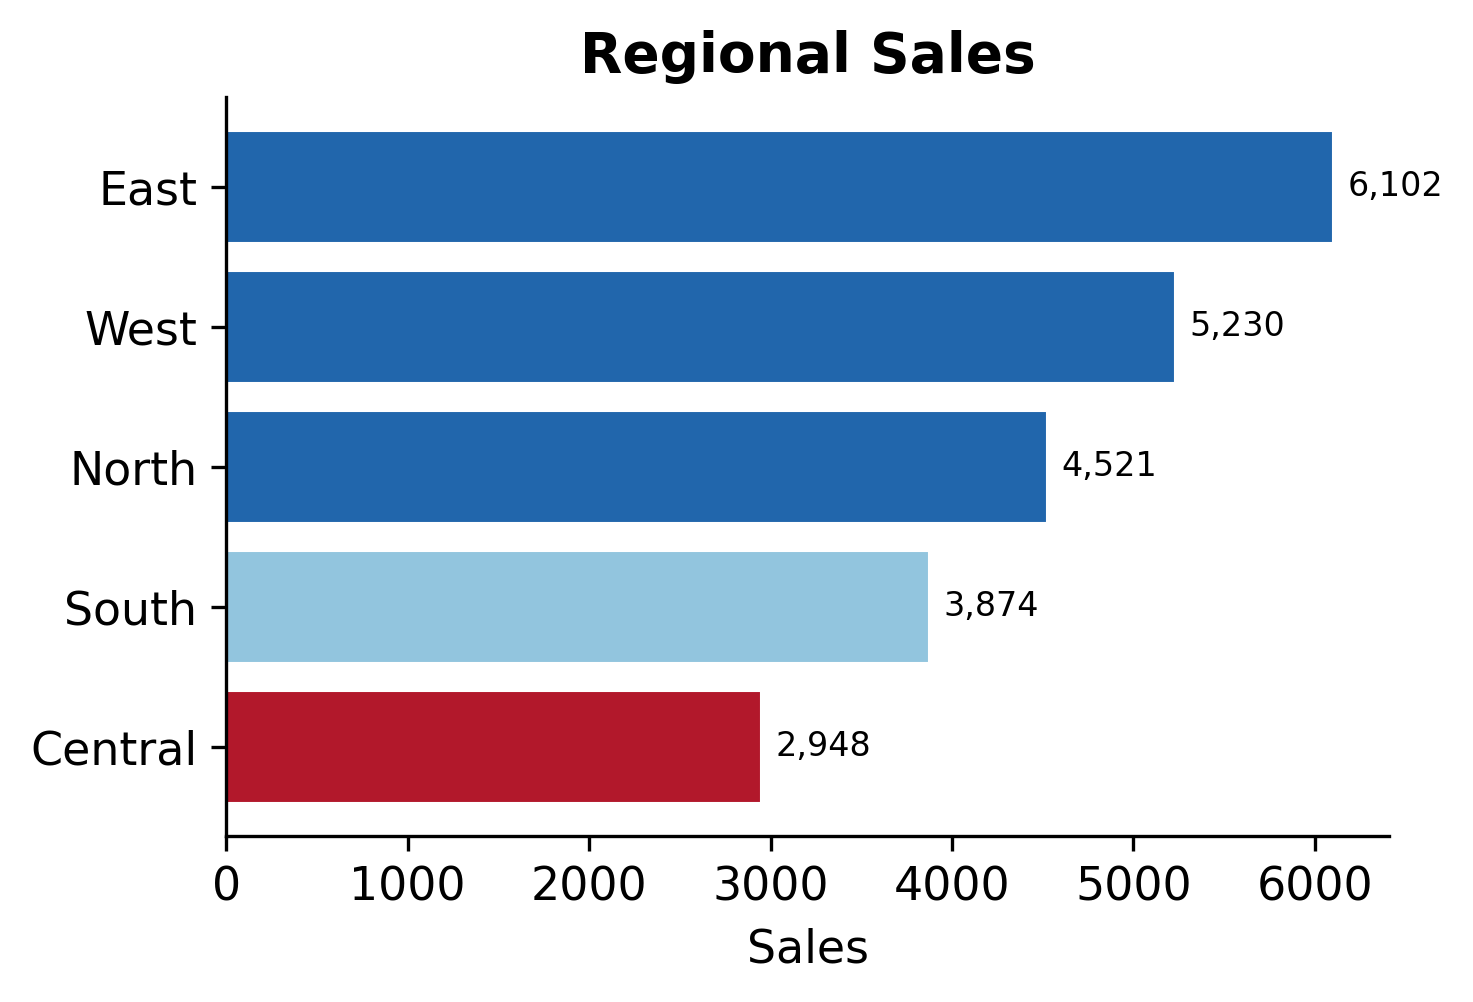
\includegraphics[width=\textwidth]{m1_1_sales_bar.png}\\
\scriptsize East's lead is \textbf{instant}.
\end{column}
\end{columns}
\end{frame}

% ── 5 ──
\begin{frame}{The Human Visual System}\smark{5/300}
\begin{columns}[T]
\begin{column}{0.52\textwidth}
\begin{itemize}
    \item Retina $\to$ cortex in $<100$\,ms
    \item \textbf{Preattentive}: parallel, $<250$\,ms
    \item \textbf{Attentive}: serial, seconds
    \item $\sim$30\% of cortical neurons do vision
\end{itemize}
\end{column}
\begin{column}{0.45\textwidth}
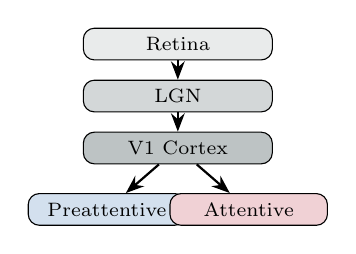
\begin{tikzpicture}[scale=0.6, every node/.style={font=\scriptsize}]
    \node[draw,rounded corners,fill=mDarkTeal!10,minimum width=2.4cm](ret)at(0,0){Retina};
    \node[draw,rounded corners,fill=mDarkTeal!20,minimum width=2.4cm](lgn)at(0,-1.1){LGN};
    \node[draw,rounded corners,fill=mDarkTeal!30,minimum width=2.4cm](v1)at(0,-2.2){V1 Cortex};
    \node[draw,rounded corners,fill=RAccent!20,minimum width=2cm](pre)at(-1.5,-3.5){Preattentive};
    \node[draw,rounded corners,fill=PyAccent!20,minimum width=2cm](att)at(1.5,-3.5){Attentive};
    \draw[-{Stealth},thick](ret)--(lgn);
    \draw[-{Stealth},thick](lgn)--(v1);
    \draw[-{Stealth},thick](v1)--(pre);
    \draw[-{Stealth},thick](v1)--(att);
\end{tikzpicture}
\end{column}
\end{columns}
\end{frame}

% ── 6 ──
\begin{frame}{Preattentive Pop-Out}\smark{6/300}
\centering
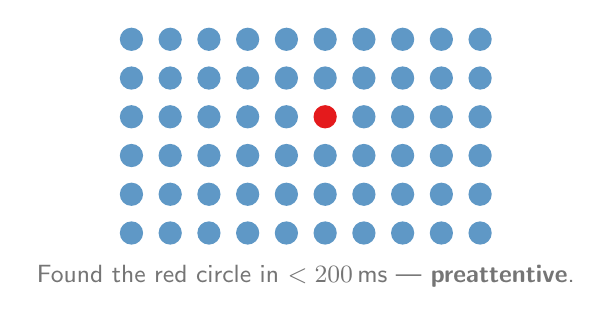
\begin{tikzpicture}[scale=0.82]
    \preattentivegrid
    \node[below,font=\small\sffamily,text=codegray] at (2.7,-0.35)
        {Found the red circle in $<200$\,ms --- \textbf{preattentive}.};
\end{tikzpicture}
\vspace{0.2cm}
\begin{exampleblock}{Data Insight}
    \scriptsize Color hue is preattentive. This is why \texttt{color} is a powerful aesthetic in \texttt{ggplot2}/\texttt{seaborn}.
\end{exampleblock}
\end{frame}

% ── 7 ──
\begin{frame}{Preattentive Feature Catalogue}\smark{7/300}
\centering\small
\begin{tabular}{@{}lll@{}}
    \toprule
    \textbf{Feature} & \textbf{Encoding} & \textbf{Grammar} \\
    \midrule
    Color hue   & Categorical grouping   & \texttt{color}/\texttt{fill} \\
    Length       & Quantitative magnitude & bar height / \texttt{y} \\
    Orientation  & Direction              & \texttt{angle} (limited) \\
    Size         & Quantitative magnitude & \texttt{size} \\
    Shape        & Categorical grouping   & \texttt{shape} \\
    \bottomrule
\end{tabular}
\vspace{0.3cm}
\begin{alertblock}{Pro-Tip}
    \scriptsize Color a target group; grey out the rest. The key comparison pops out preattentively.
\end{alertblock}
\end{frame}

% ── 8 ──
\begin{frame}{Preattentive vs.\ Attentive Exercise}\smark{8/300}
\begin{columns}[T]
\begin{column}{0.48\textwidth}
\centering\textbf{Task A: Count the 3s}\\[0.15cm]\scriptsize
\texttt{1 8 2 7 3 4 9 1 5 3}\\
\texttt{6 3 8 2 7 1 9 4 3 5}\\
\texttt{2 7 3 1 8 3 4 9 6 2}\\[0.15cm]
\normalsize\textbf{Serial search} (attentive)
\end{column}
\begin{column}{0.48\textwidth}
\centering\textbf{Task B: Count the \textcolor{dataviz1}{red} 3s}\\[0.15cm]\scriptsize
\texttt{1 8 2 7 \textcolor{dataviz1}{\textbf{3}} 4 9 1 5 \textcolor{dataviz1}{\textbf{3}}}\\
\texttt{6 \textcolor{dataviz1}{\textbf{3}} 8 2 7 1 9 4 \textcolor{dataviz1}{\textbf{3}} 5}\\
\texttt{2 7 \textcolor{dataviz1}{\textbf{3}} 1 8 \textcolor{dataviz1}{\textbf{3}} 4 9 6 2}\\[0.15cm]
\normalsize\textbf{Parallel pop-out} (preattentive)
\end{column}
\end{columns}
\end{frame}

% ── 9 ──
\begin{frame}{Gestalt Principles}\smark{9/300}
\begin{columns}[T]
\begin{column}{0.50\textwidth}
\begin{itemize}
    \item \textbf{Proximity} --- nearby elements group
    \item \textbf{Similarity} --- same color/shape $\to$ group
    \item \textbf{Continuity} --- aligned points form lines
    \item \textbf{Enclosure} --- bounded regions group
\end{itemize}
\begin{exampleblock}{Data Insight}
    \scriptsize Faceting = proximity. Color = similarity. Trend lines = continuity.
\end{exampleblock}
\end{column}
\begin{column}{0.47\textwidth}
\centering
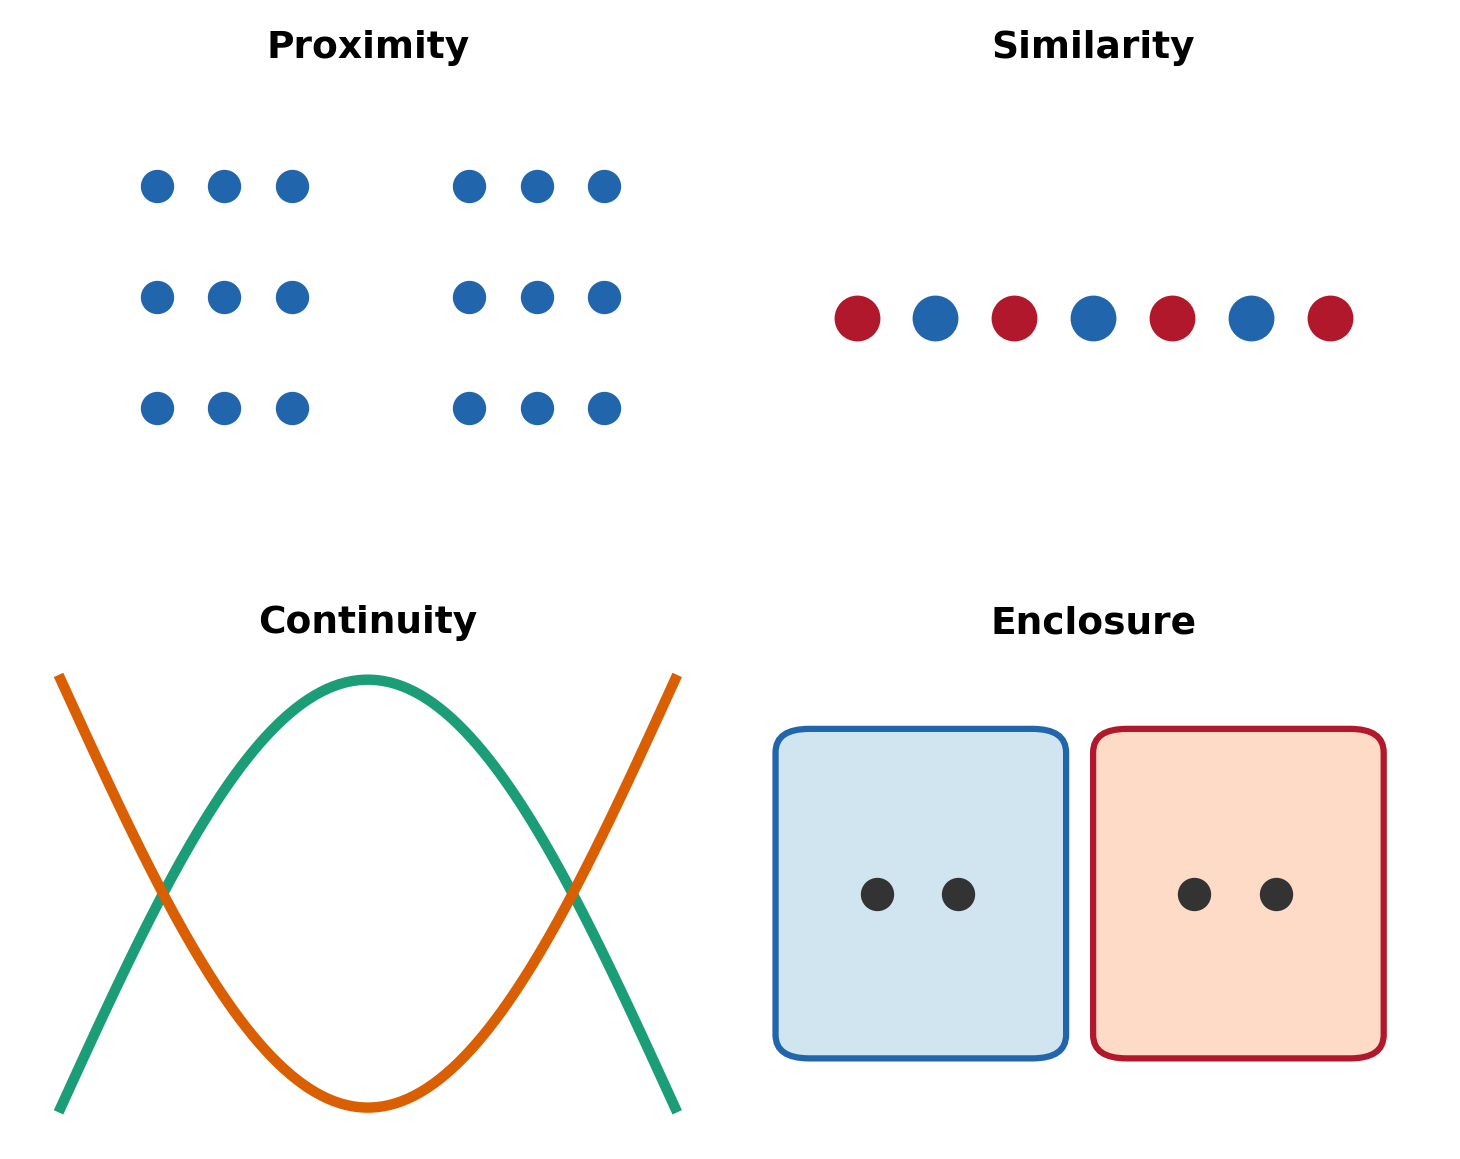
\includegraphics[width=\textwidth]{m1_1_gestalt.png}
\end{column}
\end{columns}
\end{frame}

% ── 10 ──
\begin{frame}{Anscombe's Quartet --- The Numbers Lie}\smark{10/300}
\centering\scriptsize
\begin{tabular}{@{}rr|rr|rr|rr@{}}
    \toprule
    \multicolumn{2}{c|}{\textbf{I}} & \multicolumn{2}{c|}{\textbf{II}} &
    \multicolumn{2}{c|}{\textbf{III}} & \multicolumn{2}{c}{\textbf{IV}} \\
    $x$ & $y$ & $x$ & $y$ & $x$ & $y$ & $x$ & $y$ \\
    \midrule
    10&8.04 & 10&9.14 & 10&7.46 &  8&6.58 \\
     8&6.95 &  8&8.14 &  8&6.77 &  8&5.76 \\
    13&7.58 & 13&8.74 & 13&12.74&  8&7.71 \\
     9&8.81 &  9&8.77 &  9&7.11 &  8&8.84 \\
    11&8.33 & 11&9.26 & 11&7.81 &  8&8.47 \\
    14&9.96 & 14&8.10 & 14&8.84 &  8&7.04 \\
     6&7.24 &  6&6.13 &  6&6.08 &  8&5.25 \\
     4&4.26 &  4&3.10 &  4&5.39 & 19&12.50\\
    12&10.84& 12&9.13 & 12&8.15 &  8&5.56 \\
     7&4.82 &  7&7.26 &  7&6.42 &  8&7.91 \\
     5&5.68 &  5&4.74 &  5&5.73 &  8&6.89 \\
    \bottomrule
\end{tabular}\\[0.2cm]
\normalsize All four: $\bar{x}=9$, $\bar{y}\approx7.5$, $r\approx0.816$. \textbf{Same dataset?}
\end{frame}

% ── 11 ──
\begin{frame}{Anscombe's Quartet --- The Plot}\smark{11/300}
\centering
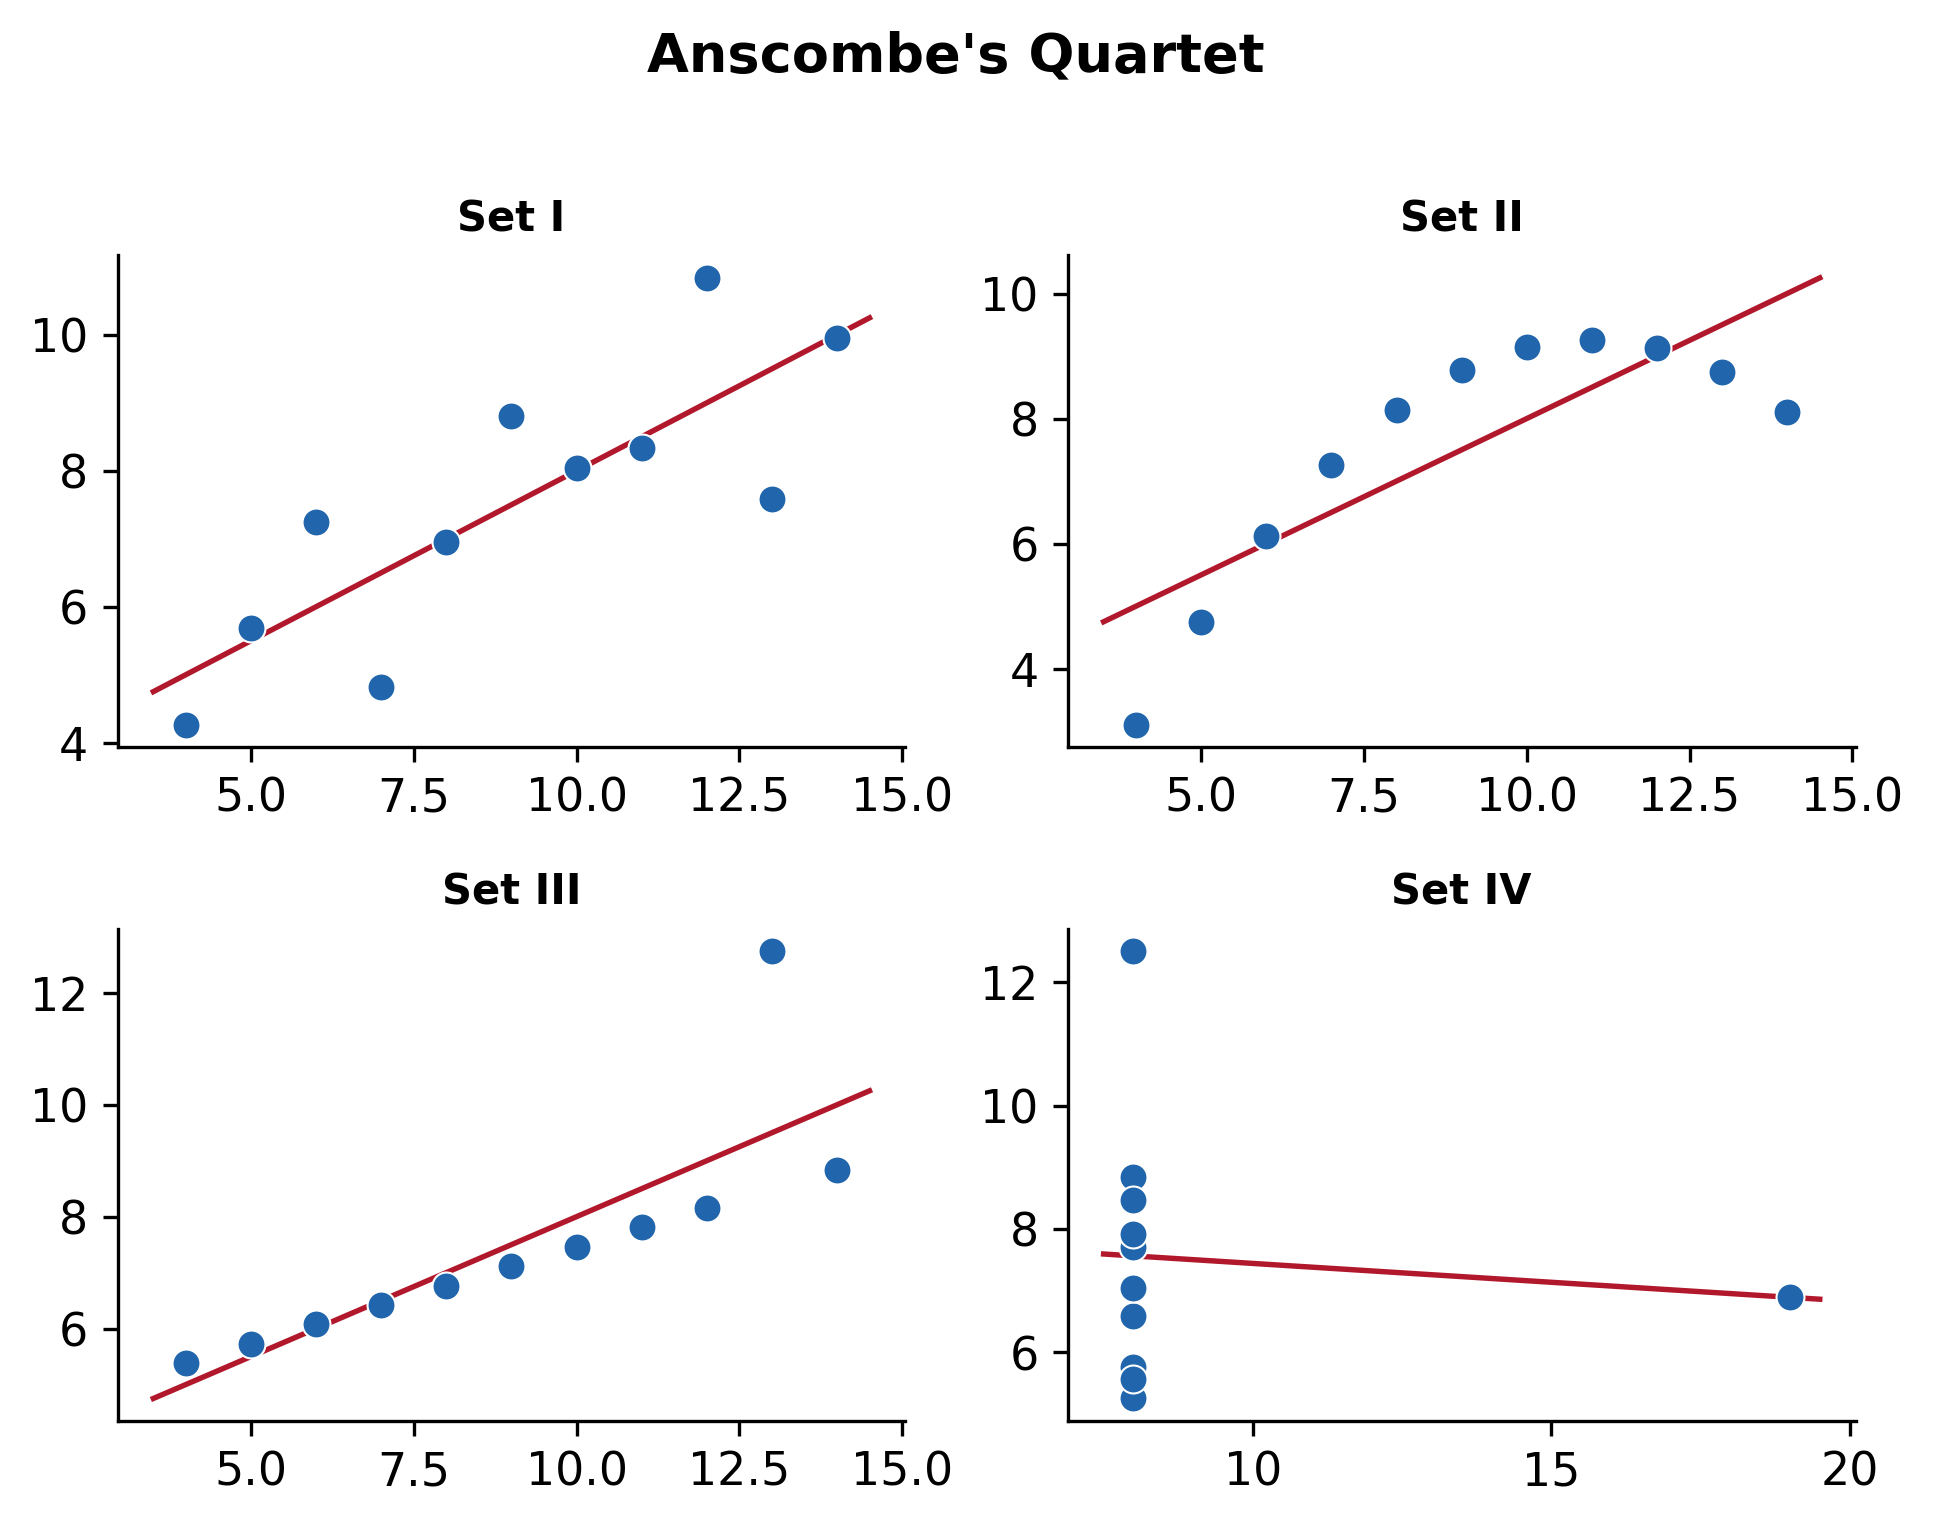
\includegraphics[width=0.82\textwidth]{m1_1_anscombe.png}
\vspace{0.2cm}
\begin{exampleblock}{Data Insight}
    \scriptsize Identical statistics, radically different structure. \textbf{Always plot your data} (Anscombe, 1973).
\end{exampleblock}
\end{frame}

% ── 12 ──
\begin{frame}[fragile]{Anscombe --- \Rlang}\smark{12/300}
\begin{columns}[T]
\begin{column}{0.55\textwidth}
\begin{lstlisting}[style=Rstyle]
ansc <- anscombe |>
  pivot_longer(everything(),
    names_to  = c(".value","set"),
    names_pattern = "(.)(.)")

ggplot(ansc, aes(x, y)) +
  geom_point(color="#2166AC") +
  geom_smooth(method="lm",
    se=FALSE, color="#B2182B") +
  facet_wrap(~set, ncol=2)
\end{lstlisting}
\scriptref{scripts/m1\_1\_anscombe.R}
\end{column}
\begin{column}{0.42\textwidth}
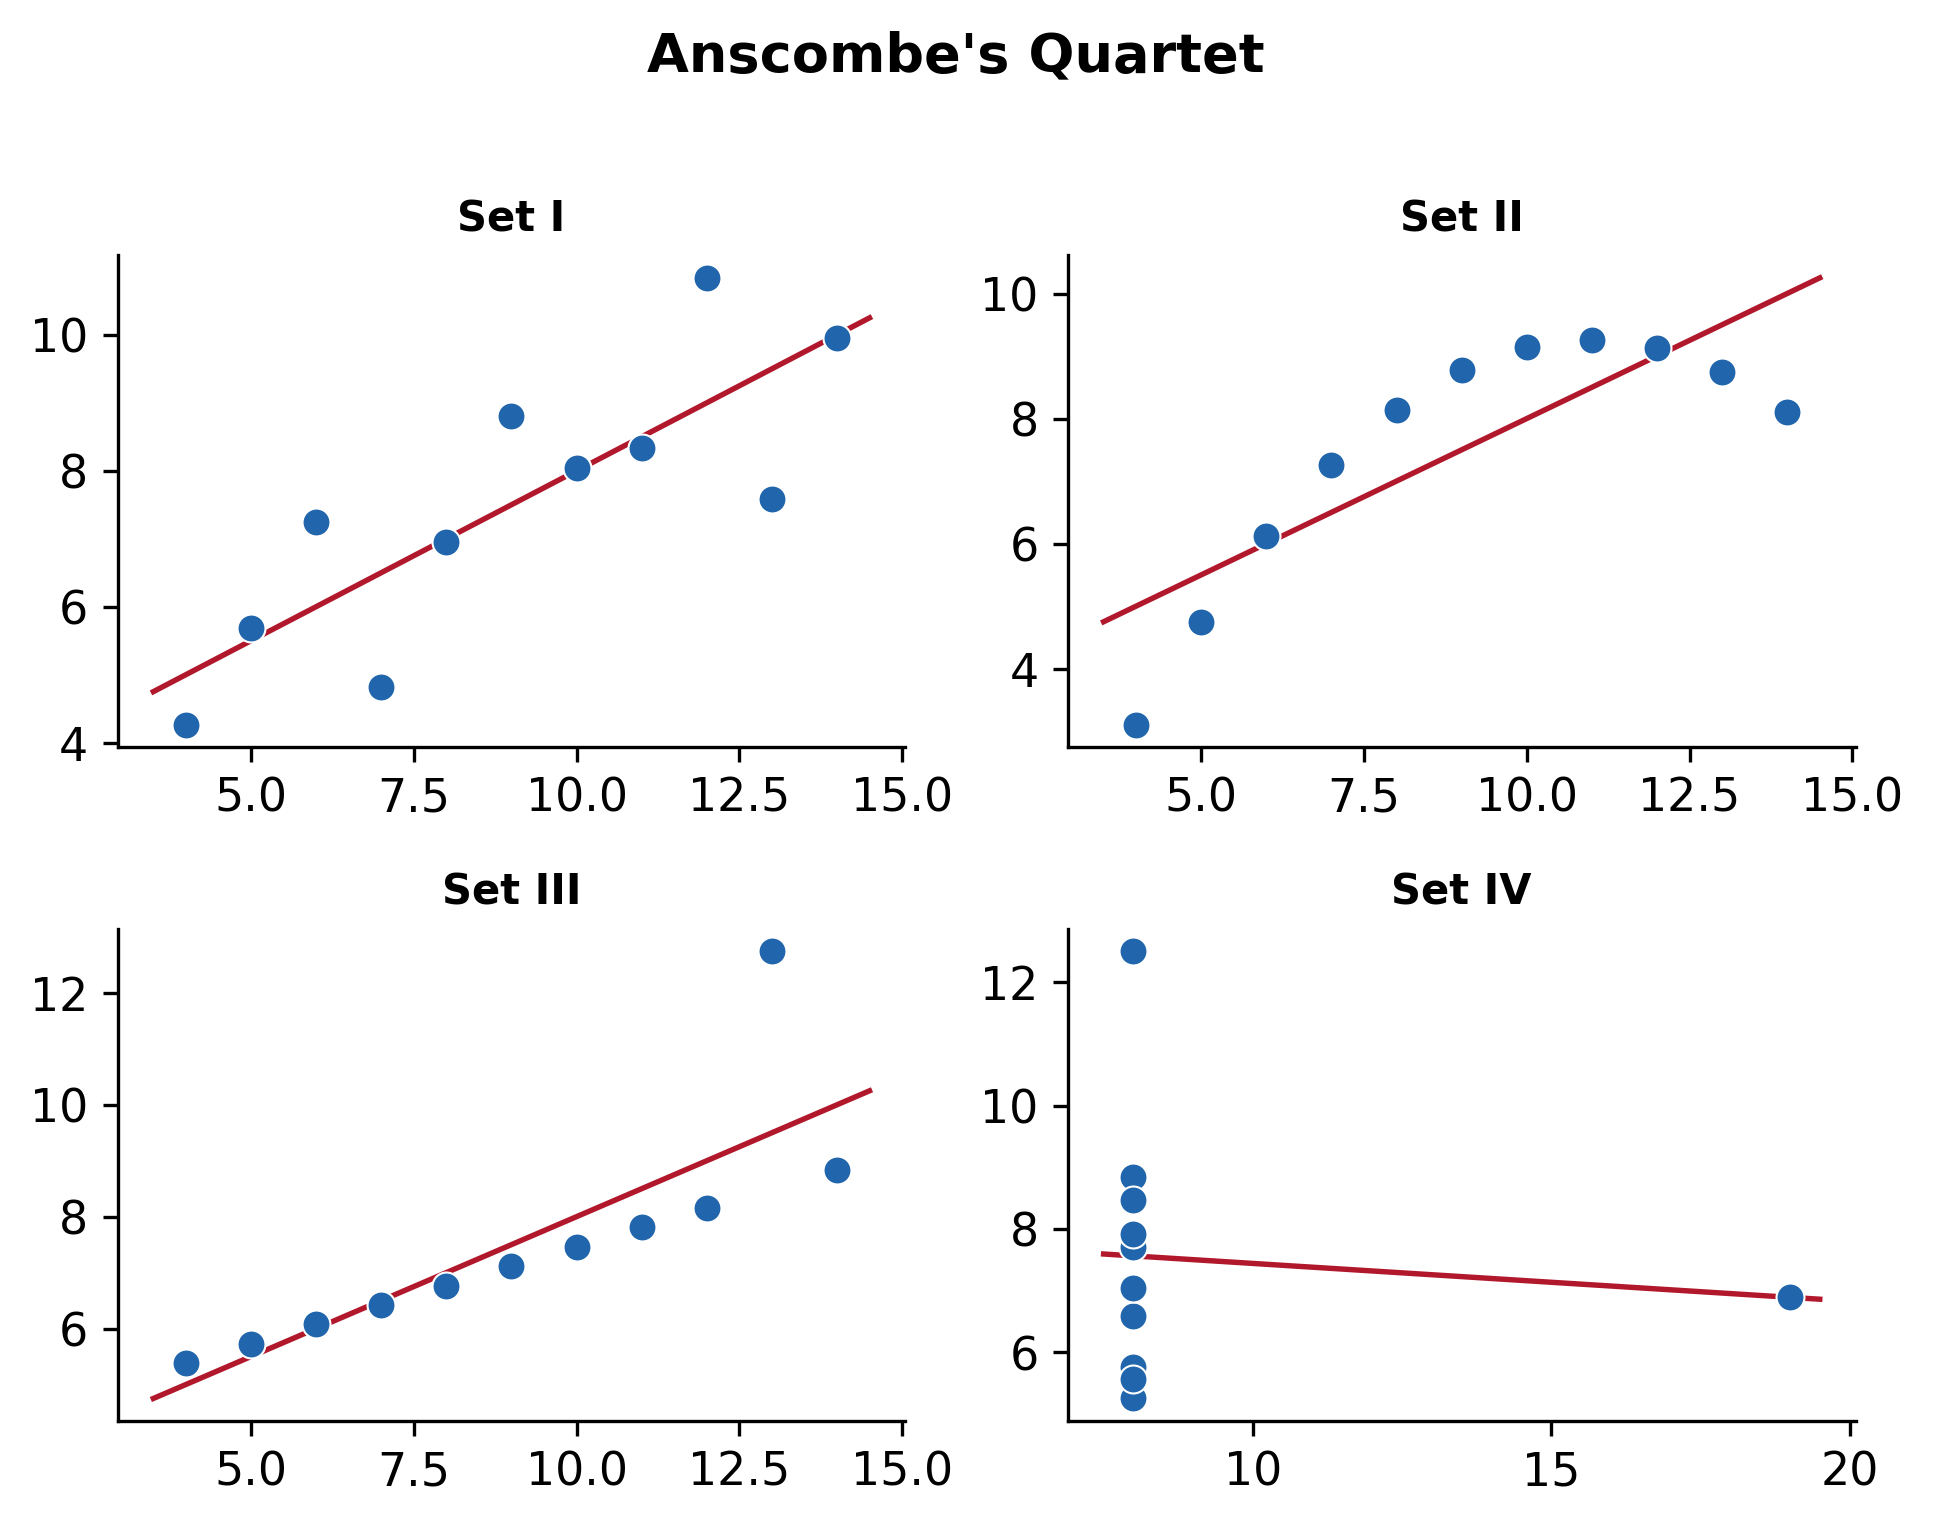
\includegraphics[width=\textwidth]{m1_1_anscombe.png}
\begin{alertblock}{Pro-Tip}
    \scriptsize \texttt{names\_pattern="(.)(.)"} splits \texttt{x1} into column \texttt{x} and set \texttt{1}.
\end{alertblock}
\end{column}
\end{columns}
\end{frame}

% ── 13 ──
\begin{frame}[fragile]{Anscombe --- \Python}\smark{13/300}
\begin{columns}[T]
\begin{column}{0.55\textwidth}
\begin{lstlisting}[style=Pystyle]
df = sns.load_dataset("anscombe")

g = sns.lmplot(
    data=df, x="x", y="y",
    col="dataset", col_wrap=2,
    ci=None,
    scatter_kws={"color":"#2166AC"},
    line_kws={"color":"#B2182B"},
    height=3)
\end{lstlisting}
\scriptref{scripts/m1\_1\_anscombe.py}
\end{column}
\begin{column}{0.42\textwidth}
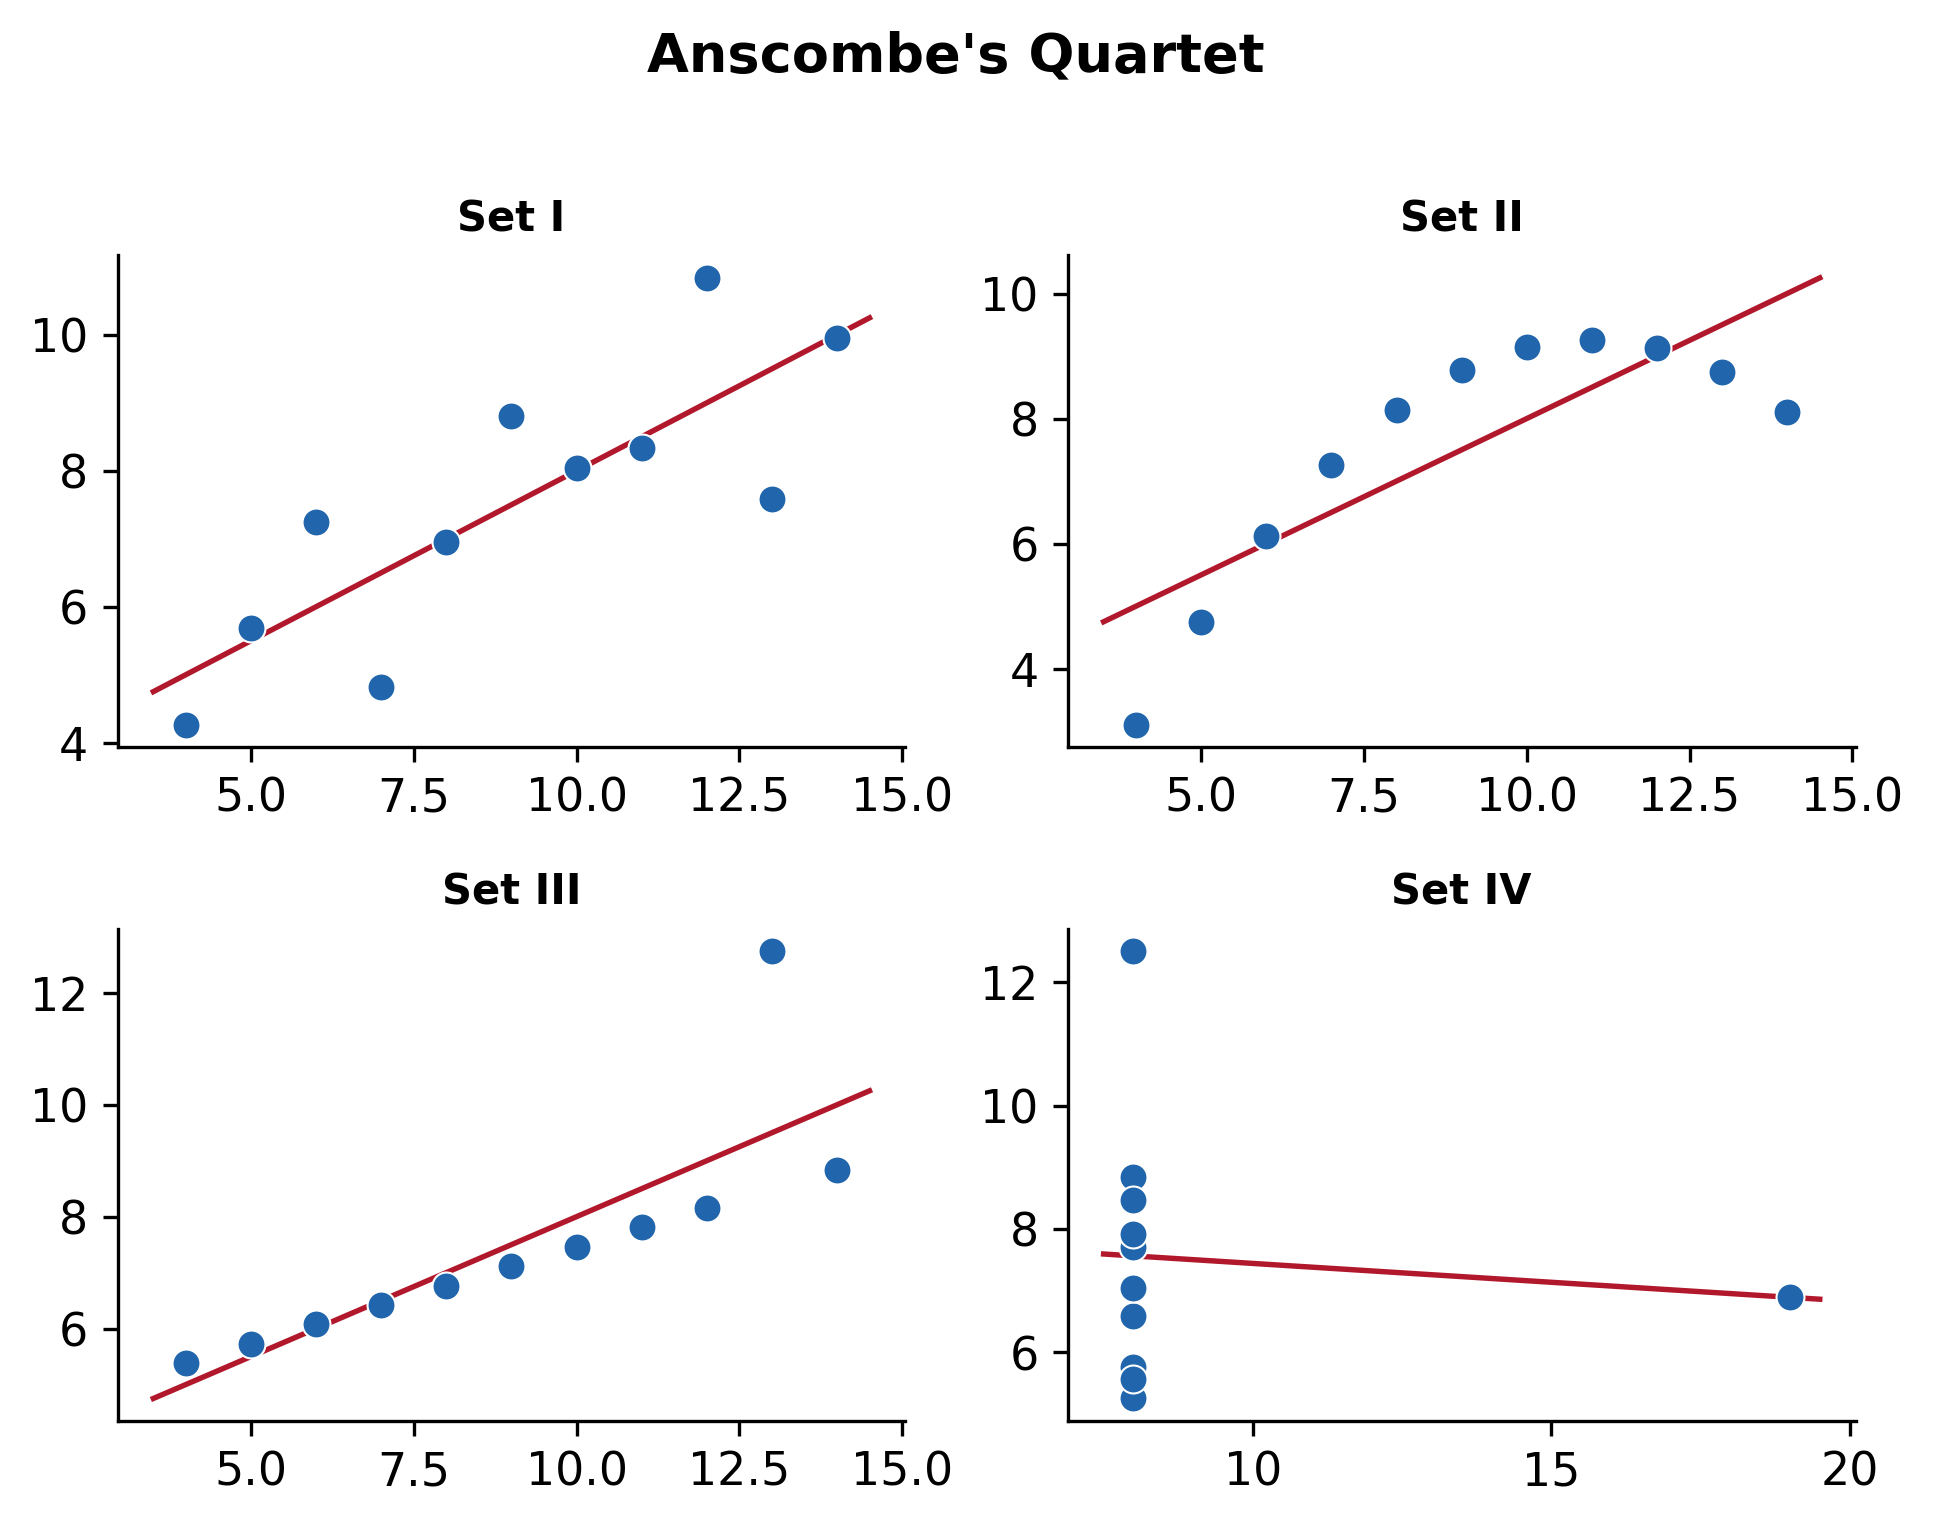
\includegraphics[width=\textwidth]{m1_1_anscombe.png}
\begin{alertblock}{Pro-Tip}
    \scriptsize \texttt{lmplot()} = scatter + OLS. \texttt{ci=None} hides confidence bands.
\end{alertblock}
\end{column}
\end{columns}
\end{frame}

% ── 14 ──
\begin{frame}{Datasaurus Dozen}\smark{14/300}
\begin{columns}[T]
\begin{column}{0.48\textwidth}
\begin{itemize}
    \item 13 datasets, \textbf{identical} $\bar{x}$, $s$, $r$
    \item T-Rex, star, circle, slant lines
    \item Simulated annealing (Matejka \& Fitzmaurice, 2017)
\end{itemize}
\end{column}
\begin{column}{0.48\textwidth}
\centering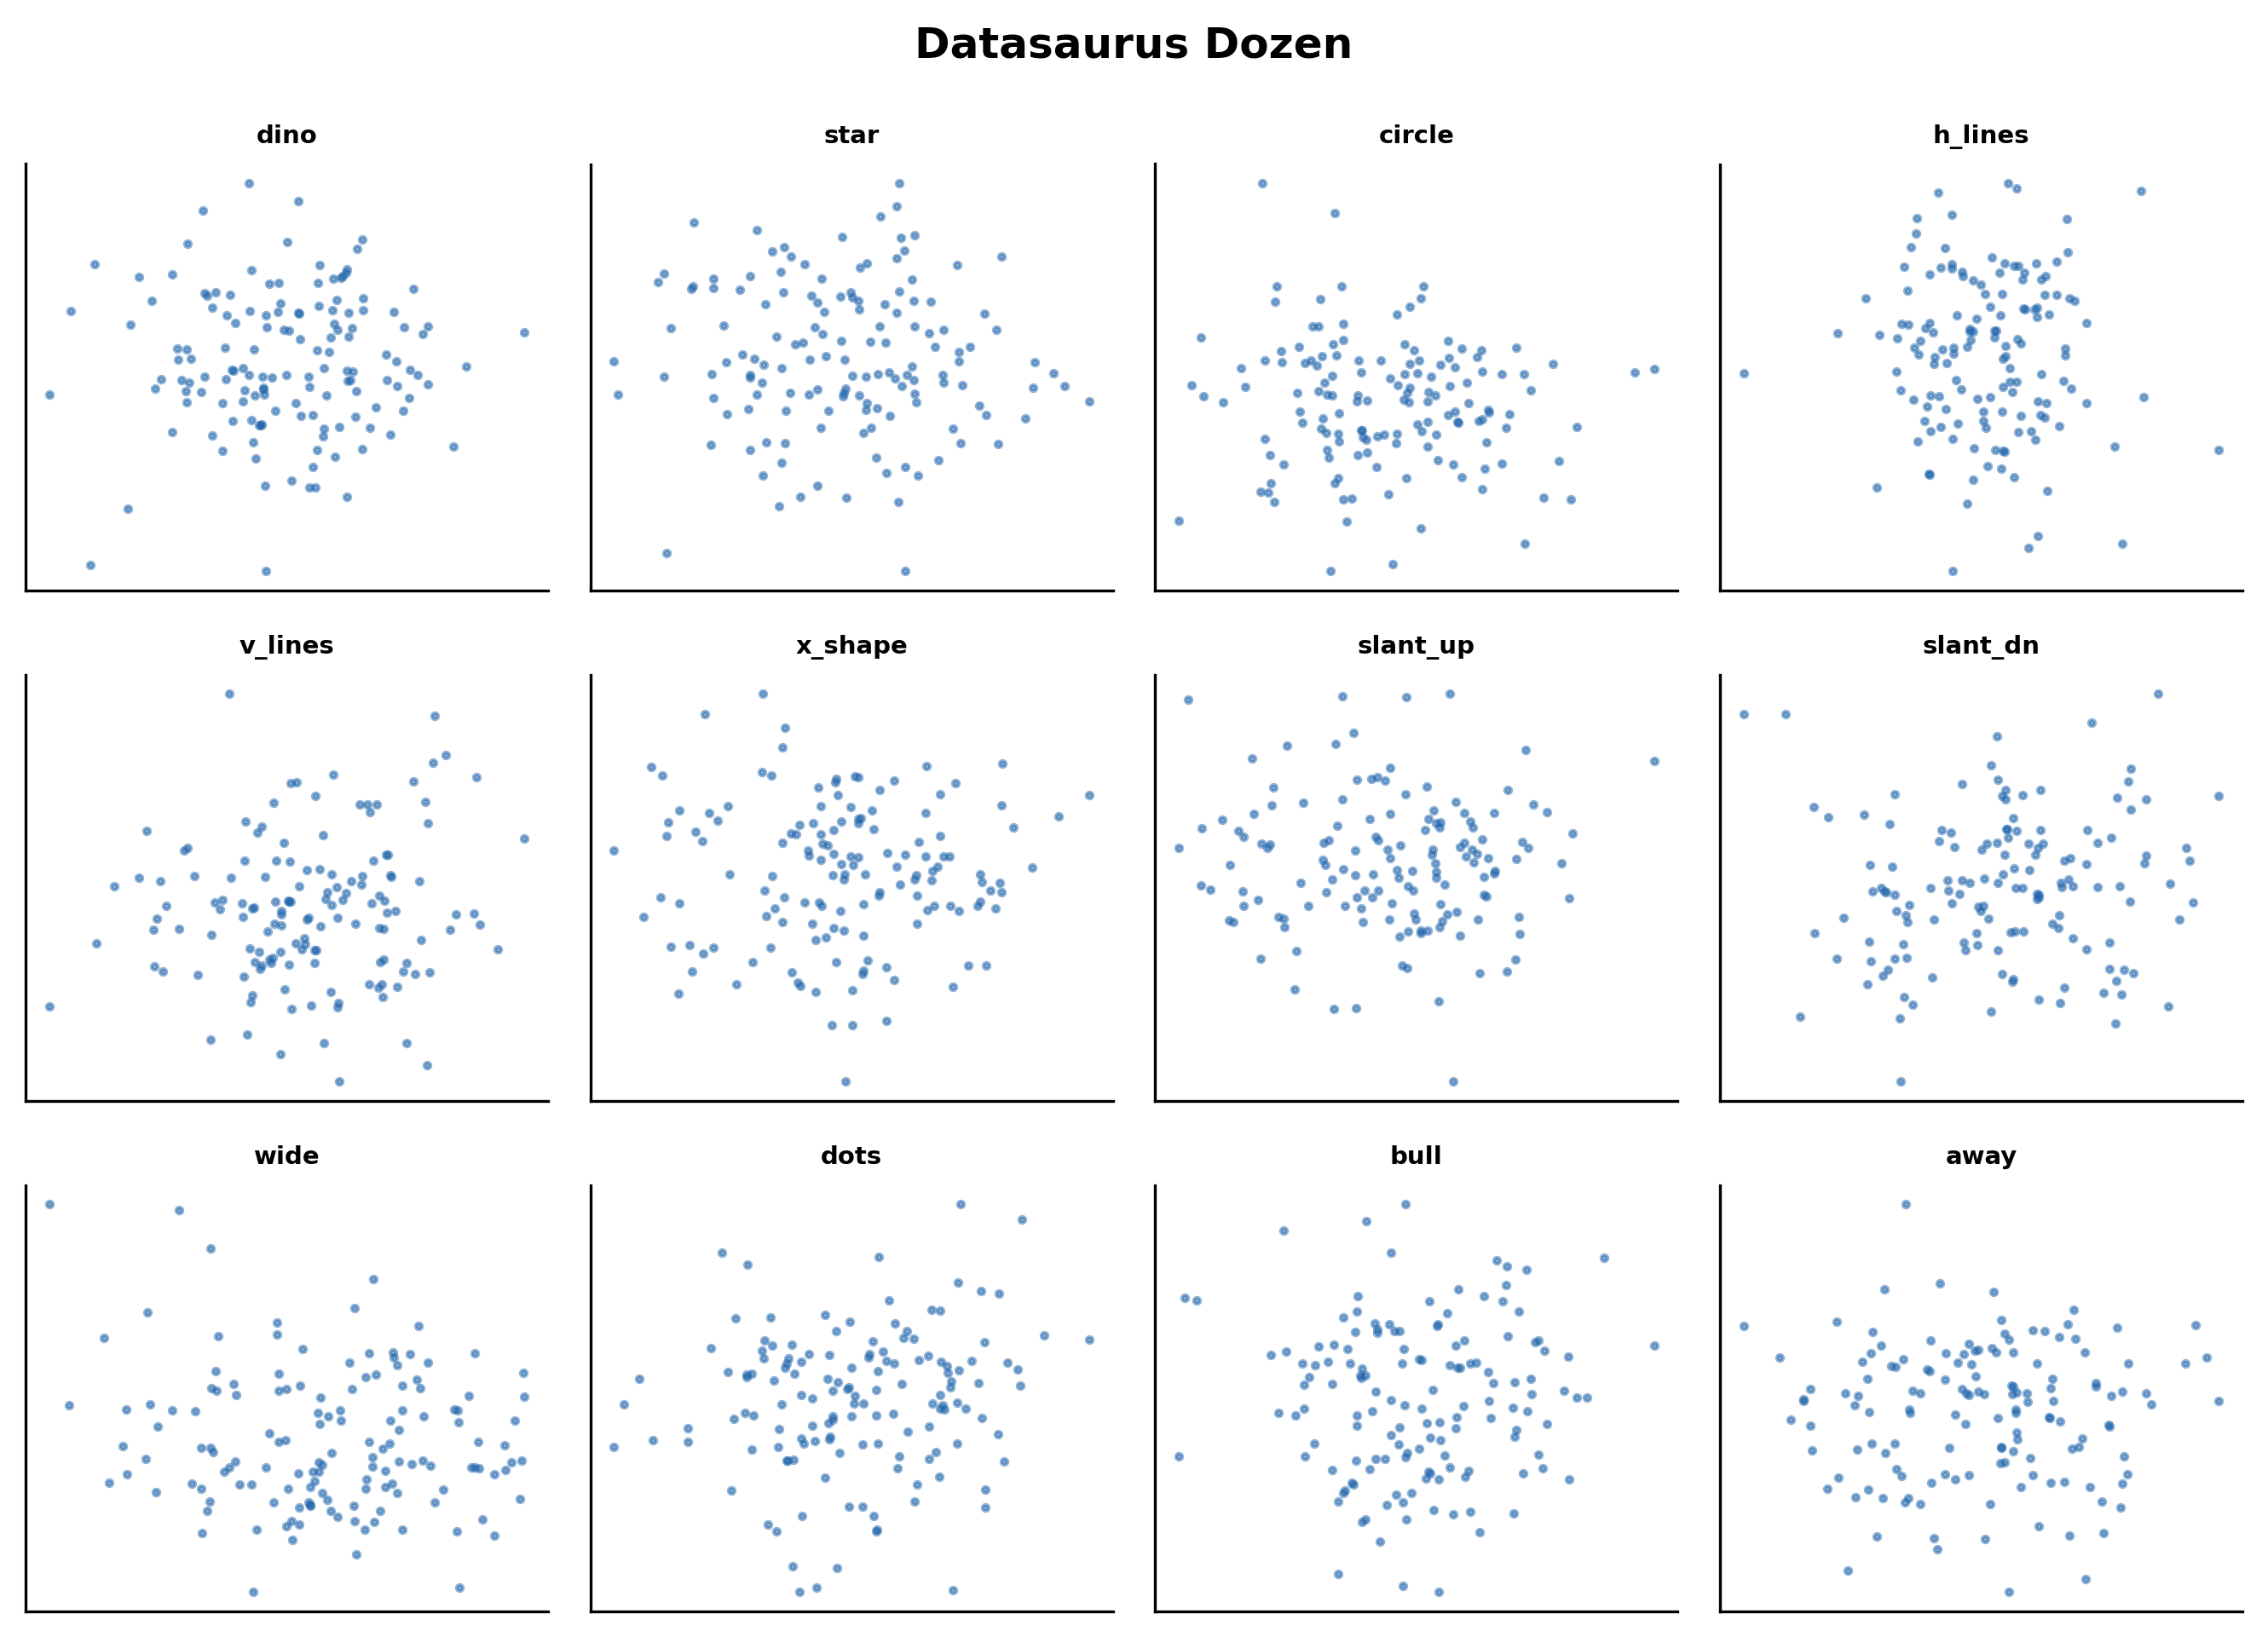
\includegraphics[width=\textwidth]{m1_1_datasaurus.png}
\end{column}
\end{columns}
\end{frame}

% ── 15 ──
\begin{frame}[fragile]{Datasaurus --- \Rlang}\smark{15/300}
\begin{columns}[T]
\begin{column}{0.55\textwidth}
\begin{lstlisting}[style=Rstyle]
library(datasauRus)
ggplot(datasaurus_dozen,
       aes(x, y)) +
  geom_point(alpha=0.6, size=0.8,
             color="#2166AC") +
  facet_wrap(~dataset, ncol=4)
\end{lstlisting}
\scriptref{scripts/m1\_1\_datasaurus.R}
\end{column}
\begin{column}{0.42\textwidth}
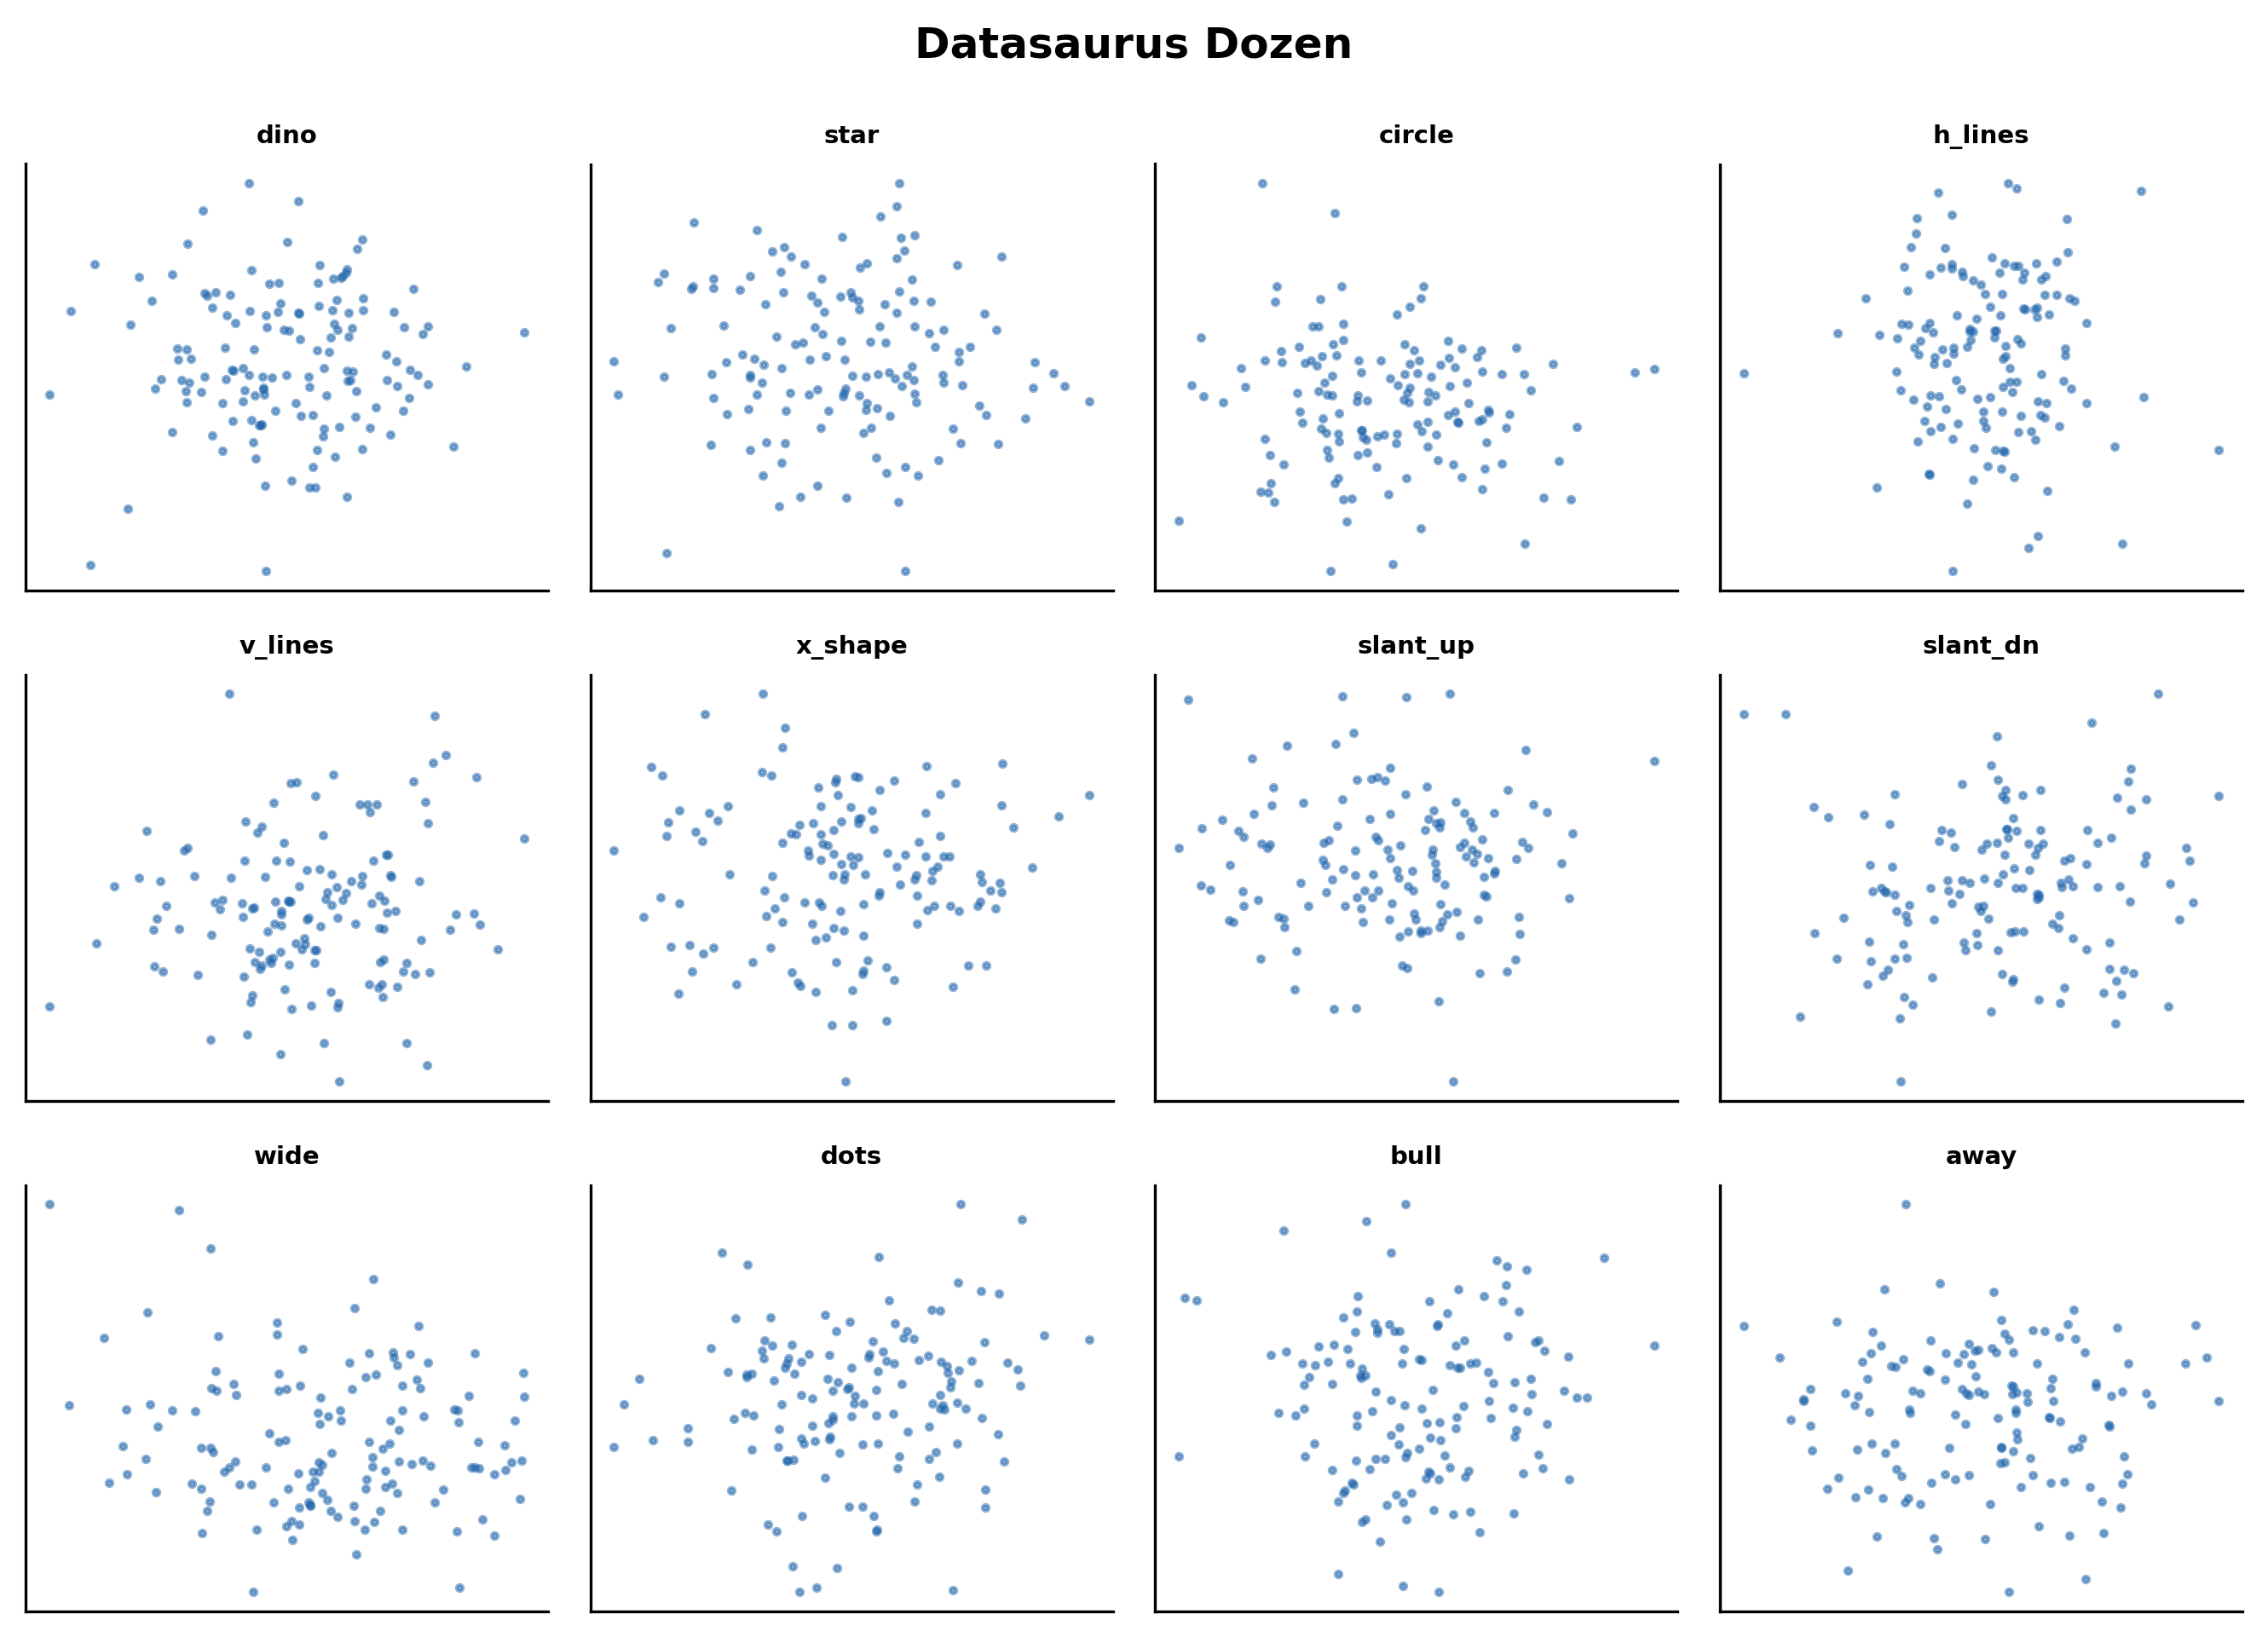
\includegraphics[width=\textwidth]{m1_1_datasaurus.png}
\end{column}
\end{columns}
\end{frame}

% ── 16 ──
\begin{frame}[fragile]{Datasaurus --- \Python}\smark{16/300}
\begin{columns}[T]
\begin{column}{0.55\textwidth}
\begin{lstlisting}[style=Pystyle]
from datasaurus import datasaurus
df = datasaurus()

fig, axes = plt.subplots(4, 4)
for ax, name in zip(
    axes.flatten(),
    df["dataset"].unique()):
    sub = df[df["dataset"]==name]
    ax.scatter(sub["x"], sub["y"],
               s=8, color="#B2182B")
\end{lstlisting}
\scriptref{scripts/m1\_1\_datasaurus.py}
\end{column}
\begin{column}{0.42\textwidth}
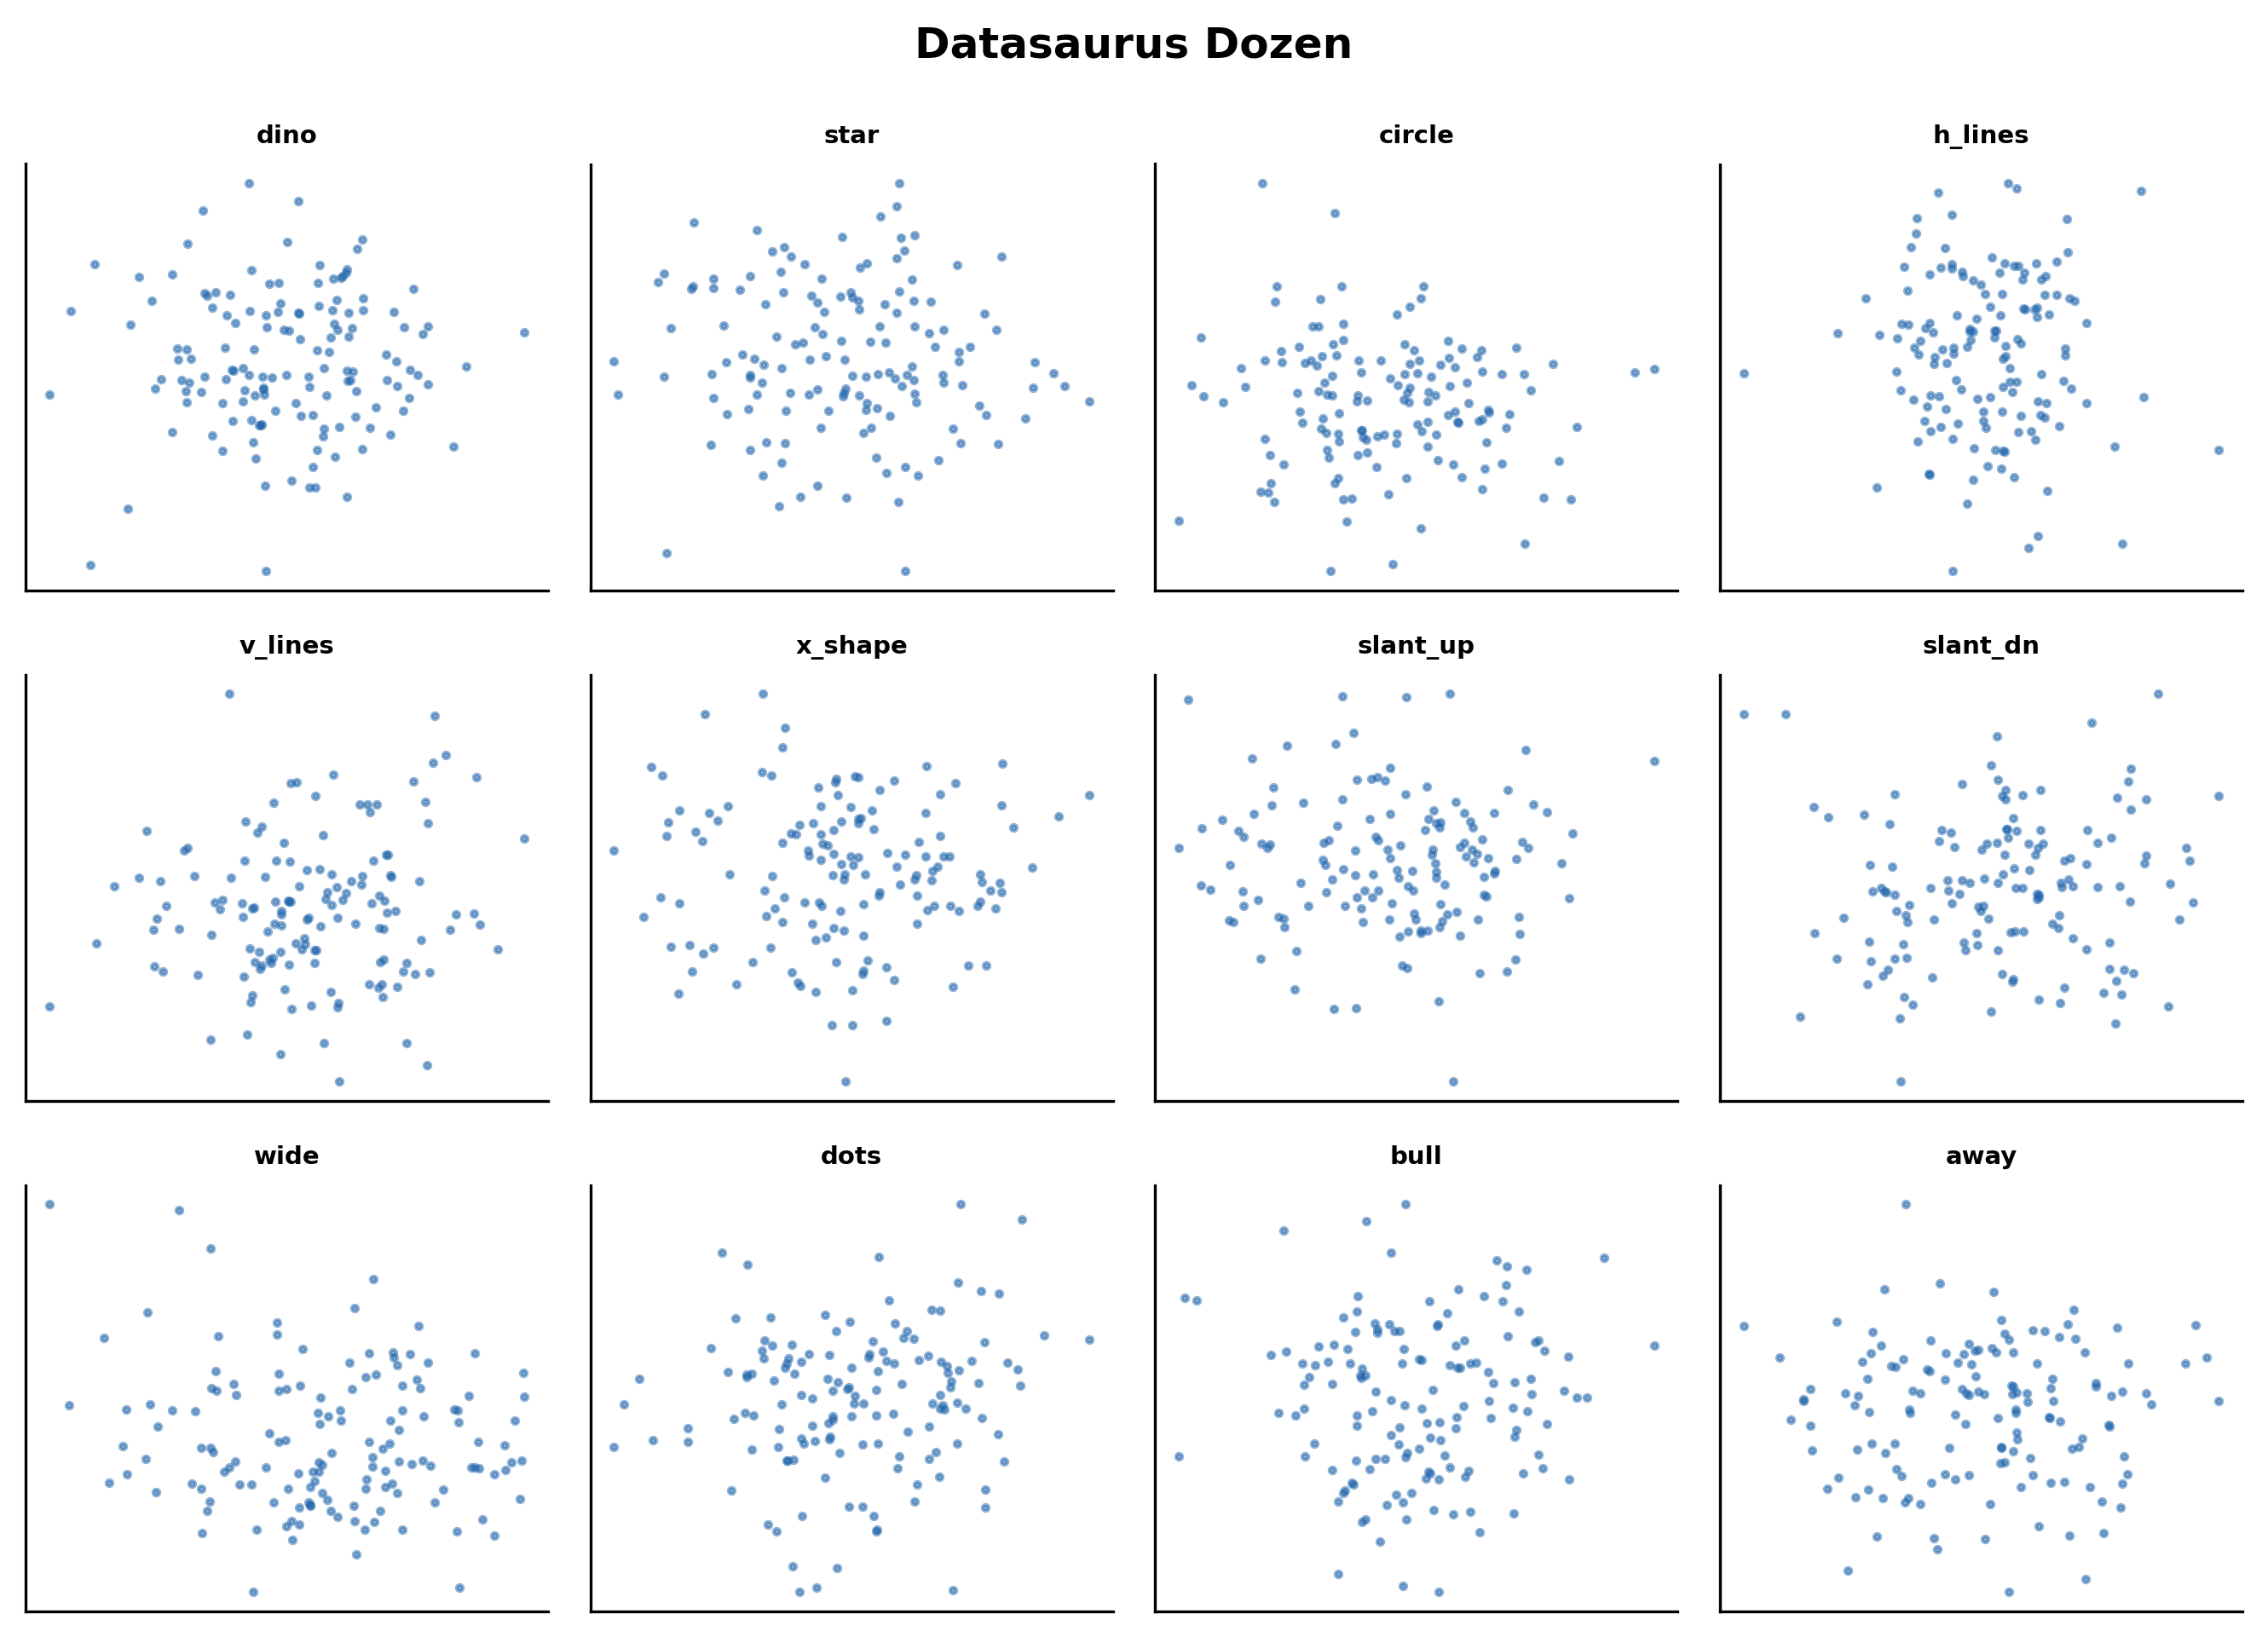
\includegraphics[width=\textwidth]{m1_1_datasaurus.png}
\end{column}
\end{columns}
\end{frame}

% ── 17 ──
\begin{frame}[fragile]{First Plot --- \Rlang\ Base Graphics}\smark{17/300}
\begin{columns}[T]
\begin{column}{0.55\textwidth}
\begin{lstlisting}[style=Rstyle]
data(iris)
plot(iris$Sepal.Length,
     iris$Sepal.Width,
     col=as.integer(iris$Species),
     pch=19, xlab="Sepal Len",
     ylab="Sepal Width")
legend("topright",
  legend=levels(iris$Species),
  col=1:3, pch=19)
\end{lstlisting}
\scriptref{scripts/m1\_1\_iris\_base.R}
\end{column}
\begin{column}{0.42\textwidth}
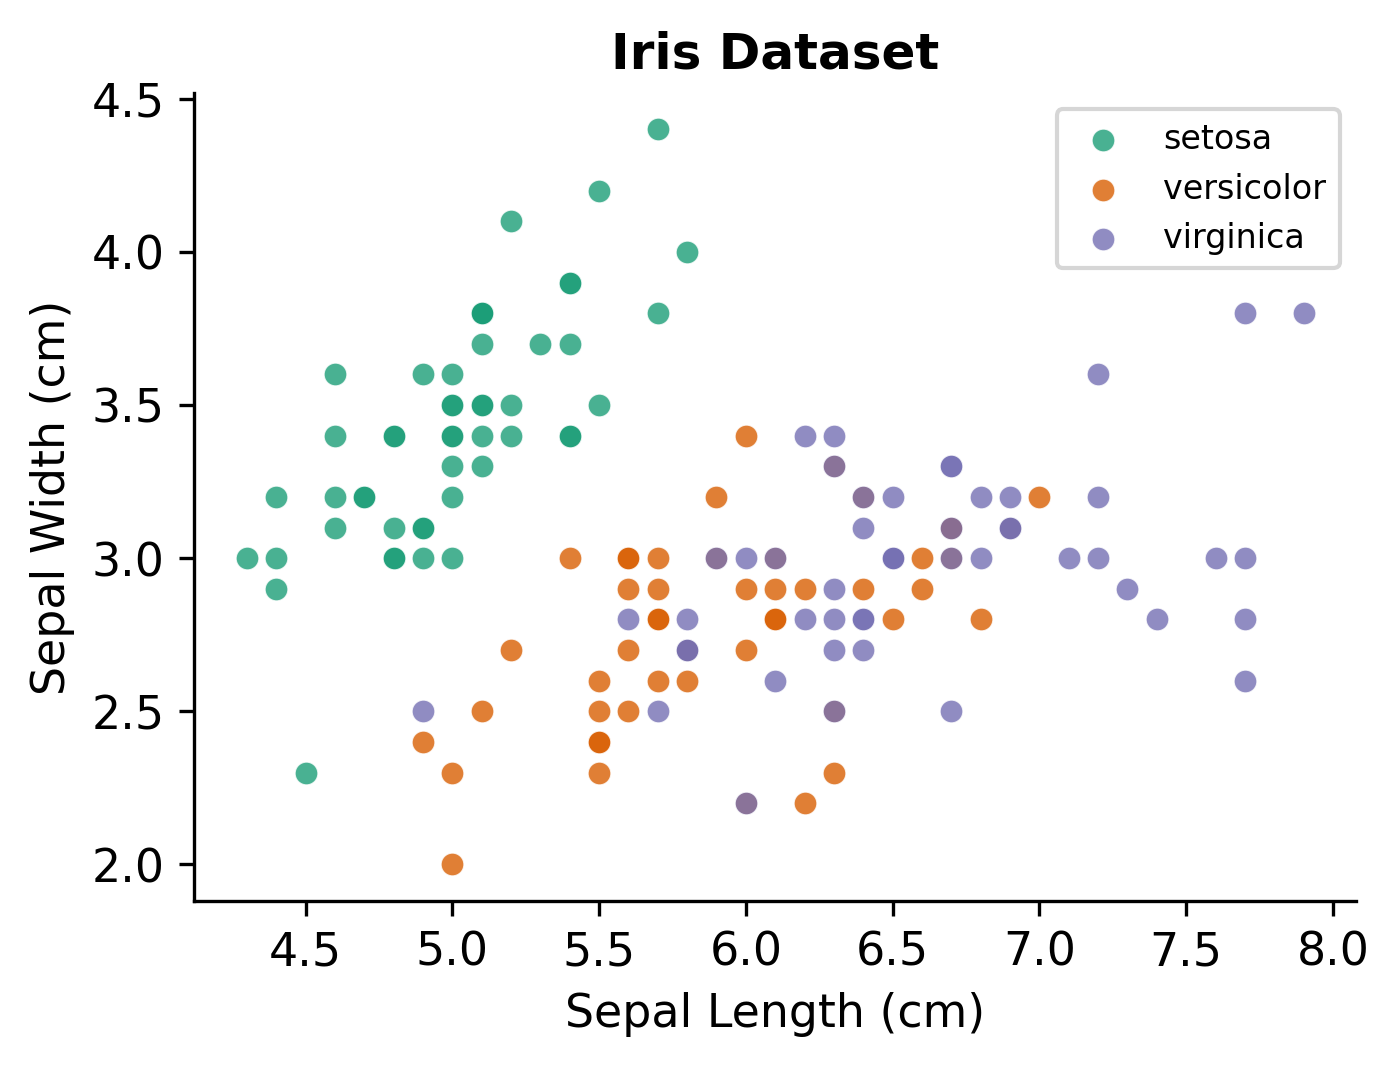
\includegraphics[width=\textwidth]{m1_1_iris.png}
\begin{exampleblock}{Data Insight}
    \scriptsize Base R = \textbf{imperative}: sequential draw commands.
\end{exampleblock}
\end{column}
\end{columns}
\end{frame}

% ── 18 ──
\begin{frame}[fragile]{First Plot --- \Python\ \texttt{matplotlib}}\smark{18/300}
\begin{columns}[T]
\begin{column}{0.55\textwidth}
\begin{lstlisting}[style=Pystyle]
from sklearn.datasets import load_iris
iris = load_iris()
fig, ax = plt.subplots()
for i, name in enumerate(
    iris.target_names):
    mask = iris.target == i
    ax.scatter(iris.data[mask,0],
               iris.data[mask,1],
               label=name)
ax.legend()
\end{lstlisting}
\scriptref{scripts/m1\_1\_iris\_mpl.py}
\end{column}
\begin{column}{0.42\textwidth}
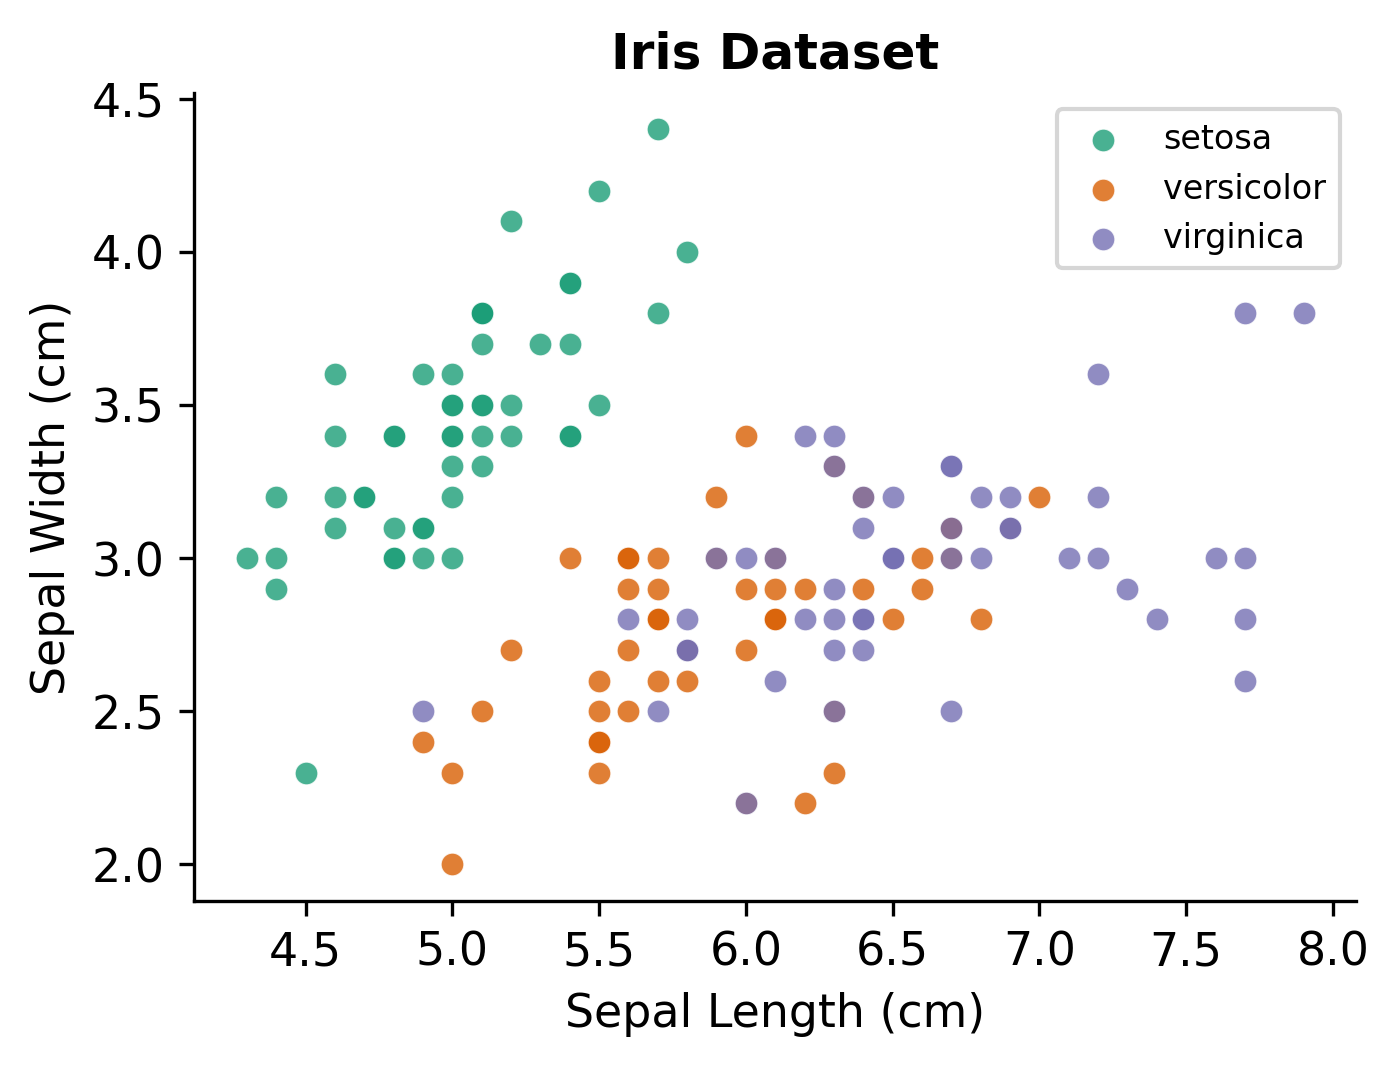
\includegraphics[width=\textwidth]{m1_1_iris.png}
\begin{exampleblock}{Data Insight}
    \scriptsize \texttt{matplotlib} = imperative. The loop mirrors R's \texttt{col=as.integer()}.
\end{exampleblock}
\end{column}
\end{columns}
\end{frame}

% ── 19 ──
\begin{frame}{Imperative vs.\ Declarative}\smark{19/300}
\centering
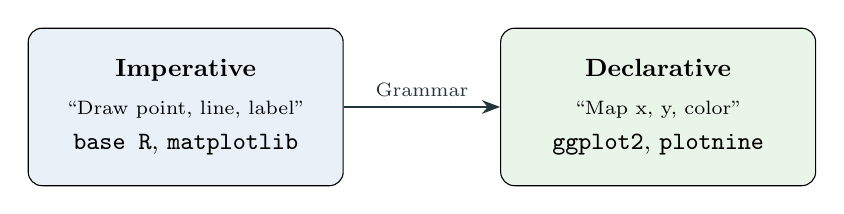
\begin{tikzpicture}[box/.style={draw,rounded corners=5pt,minimum width=4cm,
    minimum height=2cm,font=\small,align=center}]
    \node[box,fill=RAccent!10](imp)at(-3,0){\textbf{Imperative}\\[0.1cm]
        \scriptsize``Draw point, line, label''\\[0.05cm]\texttt{base R}, \texttt{matplotlib}};
    \node[box,fill=dataviz3!12](dec)at(3,0){\textbf{Declarative}\\[0.1cm]
        \scriptsize``Map x, y, color''\\[0.05cm]\texttt{ggplot2}, \texttt{plotnine}};
    \draw[-{Stealth},thick,mDarkTeal](imp)--node[above,font=\scriptsize]{Grammar}(dec);
\end{tikzpicture}
\vspace{0.3cm}
\begin{exampleblock}{Data Insight}
    \scriptsize Declarative separates \textbf{what} from \textbf{how}. Module 1.2 formalizes this.
\end{exampleblock}
\end{frame}

% ── 20 ──
\begin{frame}{Cleveland--McGill Encoding Hierarchy}\smark{20/300}
\centering\small
\begin{tabular}{@{}cl@{}}
    \toprule
    \textbf{Rank} & \textbf{Encoding Channel} \\
    \midrule
    1 & Position on common scale \textit{(most accurate)} \\
    2 & Position on non-aligned scales \\
    3 & Length \\
    4 & Angle / Slope \\
    5 & Area \\
    6 & Volume / Curvature \\
    7 & Color saturation \textit{(least accurate)} \\
    \bottomrule
\end{tabular}
\vspace{0.2cm}

{\scriptsize Cleveland \& McGill (1984). Replicated by Heer \& Bostock (2010).}
\end{frame}

% ── 21 ──
\begin{frame}{Encoding Implications}\smark{21/300}
\begin{columns}[T]
\begin{column}{0.48\textwidth}
\begin{itemize}
    \item \textbf{Position} $\to$ scatter, dot, bar
    \item \textbf{Length} $\to$ bars (align baselines!)
    \item \textbf{Angle} $\to$ pie (hard to decode)
    \item \textbf{Area} $\to$ bubbles (sparingly)
\end{itemize}
\end{column}
\begin{column}{0.48\textwidth}
\begin{alertblock}{Pro-Tip}
    \scriptsize Pick the highest-ranked encoding that fits your comparison task.
\end{alertblock}
\begin{exampleblock}{Data Insight}
    \scriptsize Bar $\to$ pie swap: $>$40\% decoding error reduction.
\end{exampleblock}
\end{column}
\end{columns}
\end{frame}

% ── 22 ──
\begin{frame}[fragile]{Encoding: Bar vs.\ Pie --- \Rlang}\smark{22/300}
\begin{columns}[T]
\begin{column}{0.55\textwidth}
\begin{lstlisting}[style=Rstyle]
p1 <- ggplot(sales,
  aes(reorder(region,-value),
      value)) +
  geom_col(fill="#2166AC")

p2 <- ggplot(sales,
  aes(x="",y=value,fill=region))+
  geom_col(width=1) +
  coord_polar("y") + theme_void()
\end{lstlisting}
\scriptref{scripts/m1\_1\_encoding.R}
\end{column}
\begin{column}{0.42\textwidth}
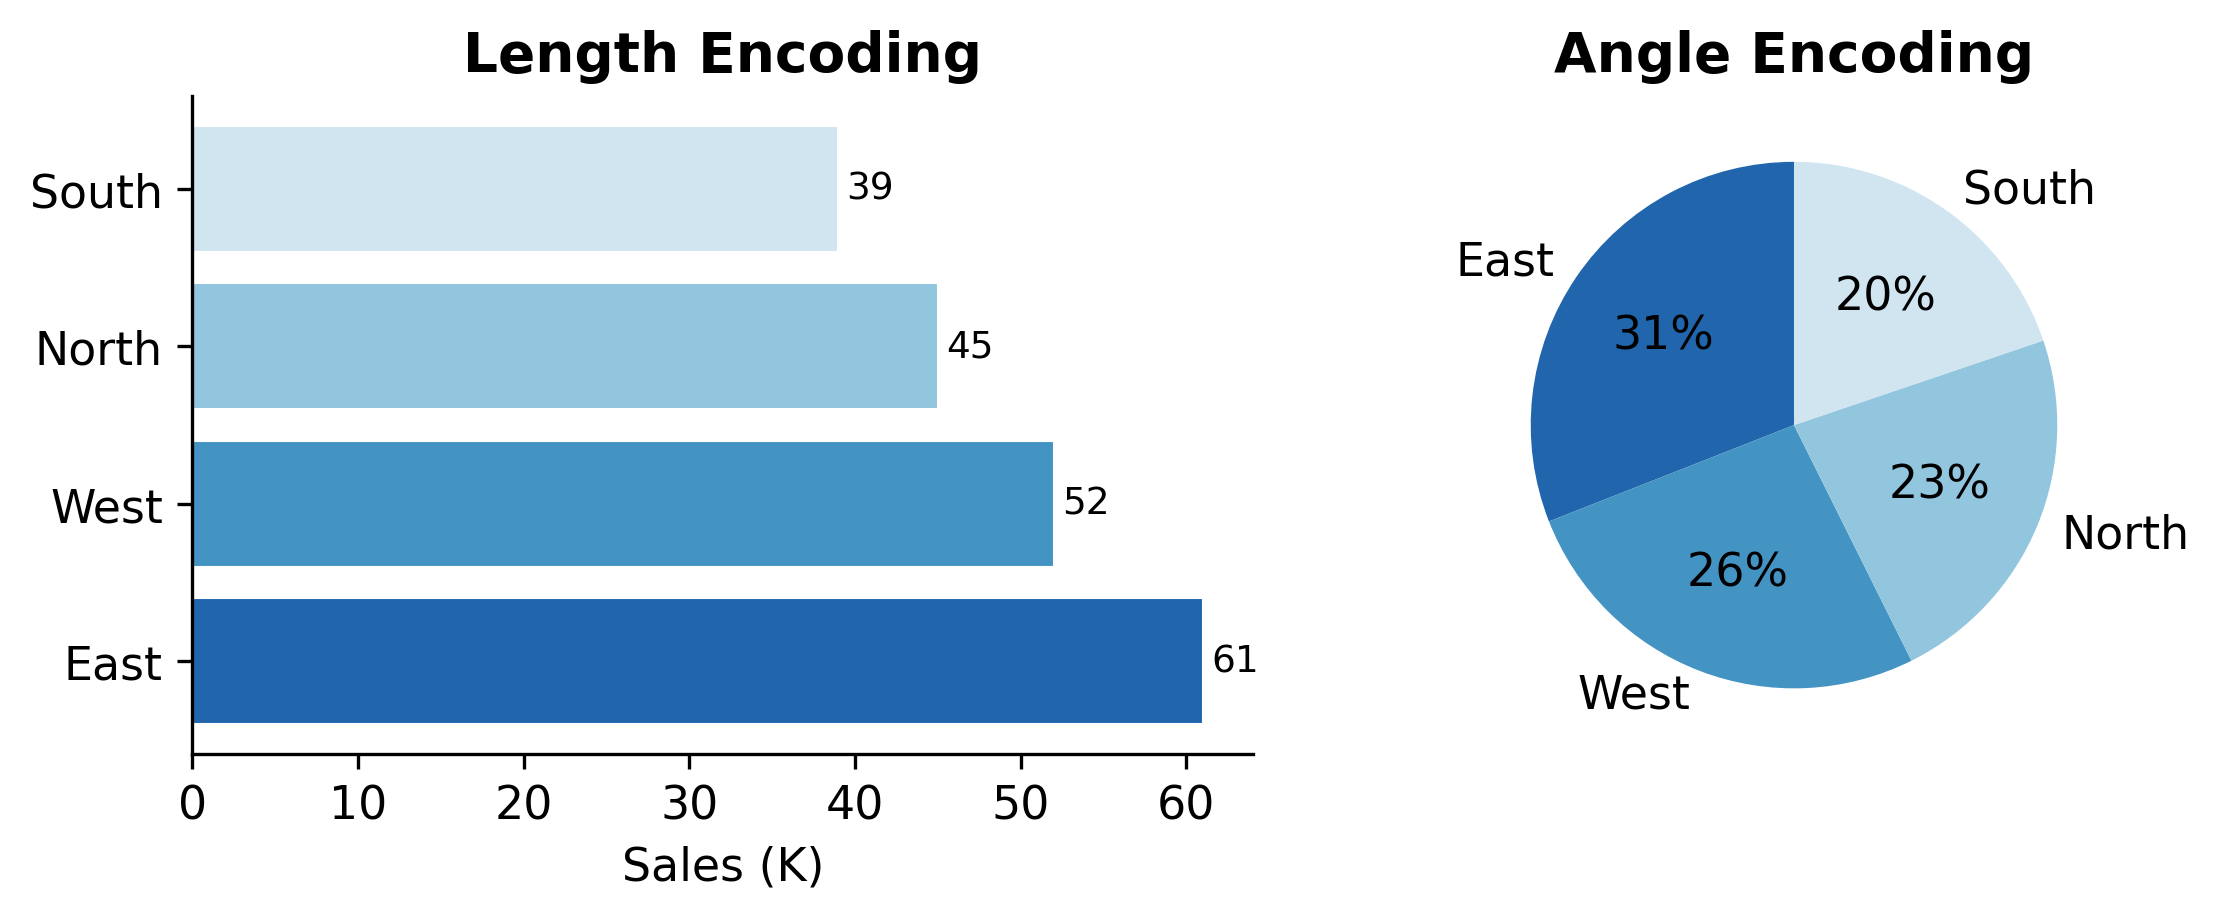
\includegraphics[width=\textwidth]{m1_1_encoding.png}
\end{column}
\end{columns}
\end{frame}

% ── 23 ──
\begin{frame}[fragile]{Encoding: Bar vs.\ Pie --- \Python}\smark{23/300}
\begin{columns}[T]
\begin{column}{0.55\textwidth}
\begin{lstlisting}[style=Pystyle]
fig,(ax1,ax2) = plt.subplots(1,2)
ax1.barh(sales["region"],
         sales["value"],
         color="#B2182B")
ax2.pie(sales["value"],
        labels=sales["region"],
        autopct="%1.0f%%")
\end{lstlisting}
\scriptref{scripts/m1\_1\_encoding.py}
\end{column}
\begin{column}{0.42\textwidth}
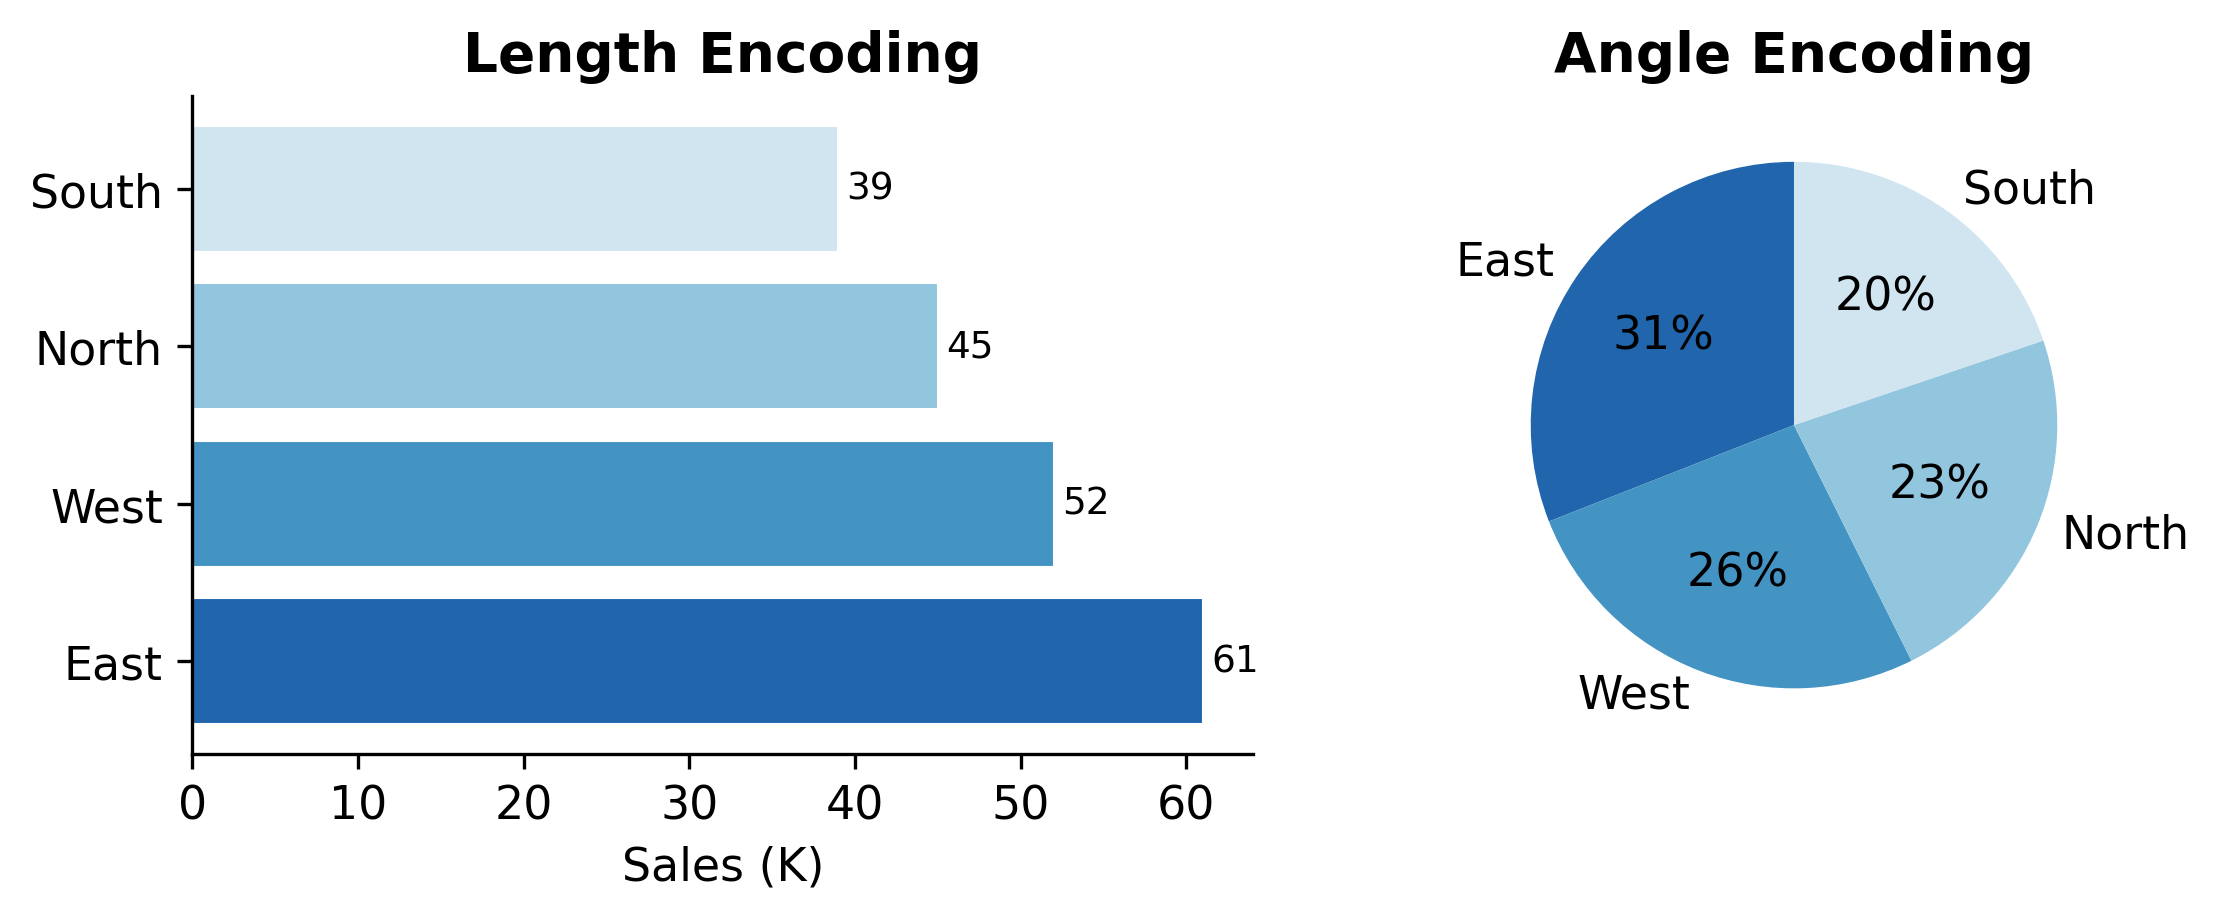
\includegraphics[width=\textwidth]{m1_1_encoding.png}
\begin{alertblock}{Pro-Tip}
    \scriptsize Sort bars by value, not alphabet. Use \texttt{barh()} for long labels.
\end{alertblock}
\end{column}
\end{columns}
\end{frame}

% ── 24 ──
\begin{frame}{Change Blindness \& Inattentional Blindness}\smark{24/300}
\begin{columns}[T]
\begin{column}{0.52\textwidth}
\begin{itemize}
    \item \textbf{Change blindness}: miss alterations across disrupted views
    \item \textbf{Inattentional blindness}: miss visible objects when focused elsewhere
    \item Dashboard rule: \textbf{no tab-switching} for critical changes
\end{itemize}
\end{column}
\begin{column}{0.45\textwidth}
\begin{alertblock}{Pro-Tip}
    \scriptsize Use \textbf{small multiples} or \textbf{animation with object constancy}.
\end{alertblock}
\begin{exampleblock}{Data Insight}
    \scriptsize Simons \& Chabris (1999): 50\% missed a gorilla in a basketball video.
\end{exampleblock}
\end{column}
\end{columns}
\end{frame}

% ── 25 ──
\begin{frame}{When Tables Beat Charts}\smark{25/300}
\begin{columns}[T]
\begin{column}{0.48\textwidth}
\textbf{Table when:}
\begin{itemize}
    \item Exact values matter
    \item $n < 5$ data points
    \item Multiple units
    \item Individual lookups
\end{itemize}
\end{column}
\begin{column}{0.48\textwidth}
\textbf{Chart when:}
\begin{itemize}
    \item Patterns/trends
    \item Group comparisons
    \item Large $n$
    \item Rapid insight needed
\end{itemize}
\end{column}
\end{columns}
\vspace{0.2cm}
\begin{exampleblock}{Data Insight}
    \scriptsize Few (2012): \textbf{lookup} $\to$ table; \textbf{comparison} $\to$ chart.
\end{exampleblock}
\end{frame}

% ── 26 ──
\begin{frame}[fragile]{Summary Stats --- \Rlang}\smark{26/300}
\begin{columns}[T]
\begin{column}{0.52\textwidth}
\begin{lstlisting}[style=Rstyle]
data(mtcars)
summary(mtcars[,c("mpg","hp","wt")])
mtcars |> group_by(cyl) |>
  summarise(mean_mpg=mean(mpg),
            sd_mpg=sd(mpg), n=n())
\end{lstlisting}
\end{column}
\begin{column}{0.45\textwidth}\scriptsize
\begin{tabular}{@{}lrrr@{}}
    \toprule
    cyl & $\bar{\text{mpg}}$ & $s$ & $n$ \\
    \midrule
    4 & 26.7 & 4.5 & 11 \\
    6 & 19.7 & 1.5 &  7 \\
    8 & 15.1 & 2.6 & 14 \\
    \bottomrule
\end{tabular}
\begin{alertblock}{Pro-Tip}
    \scriptsize \texttt{summary()} + \texttt{str()} \textbf{before} any plot.
\end{alertblock}
\end{column}
\end{columns}
\end{frame}

% ── 27 ──
\begin{frame}[fragile]{Summary Stats --- \Python}\smark{27/300}
\begin{columns}[T]
\begin{column}{0.52\textwidth}
\begin{lstlisting}[style=Pystyle]
mpg = sns.load_dataset("mpg")
mpg[["mpg","horsepower",
     "weight"]].describe()
mpg.groupby("cylinders")["mpg"]\
   .agg(["mean","std","count"])
\end{lstlisting}
\end{column}
\begin{column}{0.45\textwidth}\scriptsize
\begin{tabular}{@{}lrrr@{}}
    \toprule
    cyl & mean & std & $n$ \\
    \midrule
    3 & 20.6 & 6.5 &  4 \\
    4 & 29.3 & 5.8 & 204 \\
    6 & 20.5 & 3.8 &  84 \\
    8 & 14.9 & 3.0 & 103 \\
    \bottomrule
\end{tabular}
\begin{alertblock}{Pro-Tip}
    \scriptsize \texttt{.describe()} = count, mean, std, min, quartiles, max.
\end{alertblock}
\end{column}
\end{columns}
\end{frame}

% ── 28 ──
\begin{frame}{Tufte's Data-Ink Ratio}\smark{28/300}
\centering

\begin{tikzpicture}
    \node[draw=mDarkTeal,thick,rounded corners=6pt,fill=mDarkTeal!5,
          inner sep=10pt,font=\large]{
    $\displaystyle \text{Data-Ink Ratio}=\frac{\text{Ink for data}}{\text{Total ink}}$};
\end{tikzpicture}
\vspace{0.3cm}
\begin{columns}[T]
\begin{column}{0.48\textwidth}
\centering\textbf{Low (Chartjunk)}
\begin{itemize}
    \item 3D effects, gradients
    \item Heavy gridlines
    \item Decorative clip art
\end{itemize}
\end{column}
\begin{column}{0.48\textwidth}
\centering\textbf{High (Minimal)}
\begin{itemize}
    \item Direct labels
    \item Light/no gridlines
    \item White background
\end{itemize}
\end{column}
\end{columns}
\end{frame}

% ── 29 ──
\begin{frame}{Module 1.1 --- Takeaways}\smark{29/300}
\begin{enumerate}
    \item \textbf{Always plot your data.} Stats hide structure.
    \item \textbf{Design for preattentive processing.} Color, length, position.
    \item \textbf{Respect the encoding hierarchy.} Position $>$ Length $>$ Angle $>$ Area.
    \item \textbf{Maximize data-ink ratio.} Every pixel earns its place.
    \item \textbf{Chart vs.\ table by task.} Lookup $\to$ table; comparison $\to$ chart.
\end{enumerate}
\end{frame}

% ── 30 ──
\begin{frame}{}\smark{30/300}
\centering\vspace{1.5cm}
{\Large\textbf{Module 1.1 Complete}}\\[0.5cm]
You understand \textbf{why} we visualize and \textbf{how} the visual system processes encodings.\\[0.5cm]
\textbf{Next:} Module 1.2 --- Wilkinson's \textbf{Grammar of Graphics}.
\end{frame}

% ═══════════════════════════════════════════════════════
%  MODULE 1.2
% ═══════════════════════════════════════════════════════
\section{Module 1.2 --- The Grammar of Graphics}

% ── 31 ──
\begin{frame}{Module 1.2 --- Roadmap}\smark{31/300}
\begin{enumerate}
    \item Wilkinson's 7 Components
    \item Data \& Tidy Format
    \item Aesthetic Mappings (\texttt{aes()})
    \item Geoms \& Layering
    \item Statistical Transformations
    \item Scales \& Guides
    \item Coordinate Systems
    \item Full Pipeline: ggplot2 vs.\ plotnine vs.\ matplotlib
\end{enumerate}
\end{frame}

% ── 32 ──
\begin{frame}{A Grammar, Not a Taxonomy}\smark{32/300}
\begin{columns}[T]
\begin{column}{0.52\textwidth}
\begin{itemize}
    \item Taxonomies list types: bar, line, scatter\ldots
    \item A \textbf{grammar} decomposes into orthogonal parts
    \item $n$ geoms $\times$ $m$ stats $\times$ $k$ coords = unlimited charts
    \item Wilkinson (2005), \textit{The Grammar of Graphics}
\end{itemize}
\end{column}
\begin{column}{0.45\textwidth}
\begin{exampleblock}{Data Insight}
    \scriptsize A grammar lets you \textbf{invent} chart types by recombining components.
\end{exampleblock}
\end{column}
\end{columns}
\end{frame}

% ── 33 ──
\begin{frame}{The Seven Components}\smark{33/300}
\centering\small
\begin{tabular}{@{}clc@{}}
    \toprule
    \# & \textbf{Component} & \textbf{Required?} \\
    \midrule
    1 & \textbf{Data} --- tidy data frame             & Yes \\
    2 & \textbf{Aesthetics} --- variables $\to$ channels & Yes \\
    3 & \textbf{Geoms} --- point, line, bar\ldots      & Yes \\
    4 & \textbf{Stats} --- bin, smooth, count           & Default \\
    5 & \textbf{Scales} --- limits, palette, range      & Default \\
    6 & \textbf{Coords} --- Cartesian, polar, map       & Default \\
    7 & \textbf{Theme/Facets} --- styling, panels       & Default \\
    \bottomrule
\end{tabular}
\end{frame}

% ── 34 ──
\begin{frame}{Component 1: Data --- Tidy Requirement}\smark{34/300}
\begin{columns}[T]
\begin{column}{0.50\textwidth}
\textbf{Tidy data} (Wickham, 2014):
\begin{itemize}
    \item Each \textbf{variable} = column
    \item Each \textbf{observation} = row
    \item Each \textbf{value} = cell
\end{itemize}
\end{column}
\begin{column}{0.47\textwidth}
\begin{alertblock}{Pro-Tip}
    \scriptsize Wide data? \texttt{pivot\_longer()} (R) or \texttt{pd.melt()} (Python) first.
\end{alertblock}
\begin{exampleblock}{Data Insight}
    \scriptsize 80\% of viz effort is wrangling. Tidy = plug-and-play.
\end{exampleblock}
\end{column}
\end{columns}
\end{frame}

% ── 35 ──
\begin{frame}[fragile]{Tidy Data --- \Rlang}\smark{35/300}
\begin{columns}[T]
\begin{column}{0.55\textwidth}
\begin{lstlisting}[style=Rstyle]
wide <- tibble(
  country=c("USA","UK","Japan"),
  `2020`=c(331,67,126),
  `2021`=c(332,67,125))
tidy <- wide |>
  pivot_longer(`2020`:`2021`,
    names_to="year",
    values_to="pop_m")
\end{lstlisting}
\end{column}
\begin{column}{0.42\textwidth}\scriptsize
\begin{tabular}{@{}llr@{}}
    \toprule
    country & year & pop\_m \\
    \midrule
    USA & 2020 & 331 \\
    USA & 2021 & 332 \\
    UK  & 2020 &  67 \\
    \bottomrule
\end{tabular}
\end{column}
\end{columns}
\end{frame}

% ── 36 ──
\begin{frame}[fragile]{Tidy Data --- \Python}\smark{36/300}
\begin{columns}[T]
\begin{column}{0.55\textwidth}
\begin{lstlisting}[style=Pystyle]
tidy = wide.melt(
    id_vars="country",
    var_name="year",
    value_name="pop_m")
tidy["year"] = tidy["year"].astype(int)
\end{lstlisting}
\end{column}
\begin{column}{0.42\textwidth}
\begin{alertblock}{Pro-Tip}
    \scriptsize \texttt{pd.melt()} = Python's \texttt{pivot\_longer()}. Order differs (by variable, not id).
\end{alertblock}
\end{column}
\end{columns}
\end{frame}

% ── 37 ──
\begin{frame}{Component 2: Aesthetics (\texttt{aes})}\smark{37/300}
\centering\small
\begin{tabular}{@{}lcl@{}}
    \toprule
    \textbf{Data Variable} & $\xrightarrow{\texttt{aes()}}$ & \textbf{Visual Channel} \\
    \midrule
    \texttt{bill\_length} & $\to$ & \textbf{x} position \\
    \texttt{body\_mass}   & $\to$ & \textbf{y} position \\
    \texttt{species}      & $\to$ & \textbf{color} hue \\
    \texttt{island}       & $\to$ & \textbf{shape} \\
    \bottomrule
\end{tabular}
\vspace{0.3cm}
\begin{exampleblock}{Data Insight}
    \scriptsize \texttt{aes()} maps columns $\to$ channels. Constants go \emph{outside} \texttt{aes()}.
\end{exampleblock}
\end{frame}

% ── 38 ──
\begin{frame}[fragile]{Mapping vs.\ Setting}\smark{38/300}
\begin{columns}[T]
\begin{column}{0.48\textwidth}
\centering\textbf{Mapping}\\[0.1cm]
\begin{lstlisting}[style=Rstyle]
ggplot(penguins,
  aes(bill_length_mm,
      body_mass_g,
      color=species)) +
  geom_point()
\end{lstlisting}
\scriptsize Different color per species.
\end{column}
\begin{column}{0.48\textwidth}
\centering\textbf{Setting}\\[0.1cm]
\begin{lstlisting}[style=Rstyle]
ggplot(penguins,
  aes(bill_length_mm,
      body_mass_g)) +
  geom_point(color="#2166AC")
\end{lstlisting}
\scriptsize All points same blue.
\end{column}
\end{columns}
\vspace{0.2cm}
\begin{alertblock}{Pro-Tip}
    \scriptsize \texttt{color="blue"} \emph{inside} \texttt{aes()} = beginner mistake \#1.
\end{alertblock}
\end{frame}

% ── 39 ──
\begin{frame}[fragile]{Mapping vs.\ Setting --- \Python}\smark{39/300}
\begin{columns}[T]
\begin{column}{0.48\textwidth}
\begin{lstlisting}[style=Pystyle]
(ggplot(penguins,
   aes("bill_length_mm",
       "body_mass_g",
       color="species"))
 + geom_point())
\end{lstlisting}
\end{column}
\begin{column}{0.48\textwidth}
\begin{lstlisting}[style=Pystyle]
(ggplot(penguins,
   aes("bill_length_mm",
       "body_mass_g"))
 + geom_point(color="#B2182B"))
\end{lstlisting}
\end{column}
\end{columns}
\vspace{0.2cm}
\begin{exampleblock}{Data Insight}
    \scriptsize \texttt{plotnine} = ggplot2 syntax. Variables are \textbf{strings} in Python.
\end{exampleblock}
\end{frame}

% ── 40 ──
\begin{frame}{Component 3: Geoms}\smark{40/300}
\centering\small
\begin{tabular}{@{}lll@{}}
    \toprule
    \textbf{Geom} & \textbf{Use Case} & \textbf{Key Aesthetics} \\
    \midrule
    \texttt{geom\_point}     & Scatter     & x, y, color, size \\
    \texttt{geom\_line}      & Time series & x, y, color \\
    \texttt{geom\_col}       & Bar chart   & x, y, fill \\
    \texttt{geom\_histogram} & Distribution& x, fill \\
    \texttt{geom\_boxplot}   & Summary     & x, y, fill \\
    \texttt{geom\_smooth}    & Trend       & x, y \\
    \bottomrule
\end{tabular}
\vspace{0.2cm}
\begin{exampleblock}{Data Insight}
    \scriptsize Geoms are interchangeable. Swap \texttt{geom\_point} for \texttt{geom\_line} --- the rest stays.
\end{exampleblock}
\end{frame}

% ── 41 ──
\begin{frame}[fragile]{Layering Geoms --- \Rlang}\smark{41/300}
\begin{columns}[T]
\begin{column}{0.55\textwidth}
\begin{lstlisting}[style=Rstyle]
ggplot(mpg, aes(displ, hwy)) +
  geom_point(aes(color=class),
             alpha=0.7) +
  geom_smooth(method="loess",
              color="black") +
  geom_rug(sides="bl", alpha=0.3)
\end{lstlisting}
\scriptref{scripts/m1\_2\_layers.R}
\end{column}
\begin{column}{0.42\textwidth}
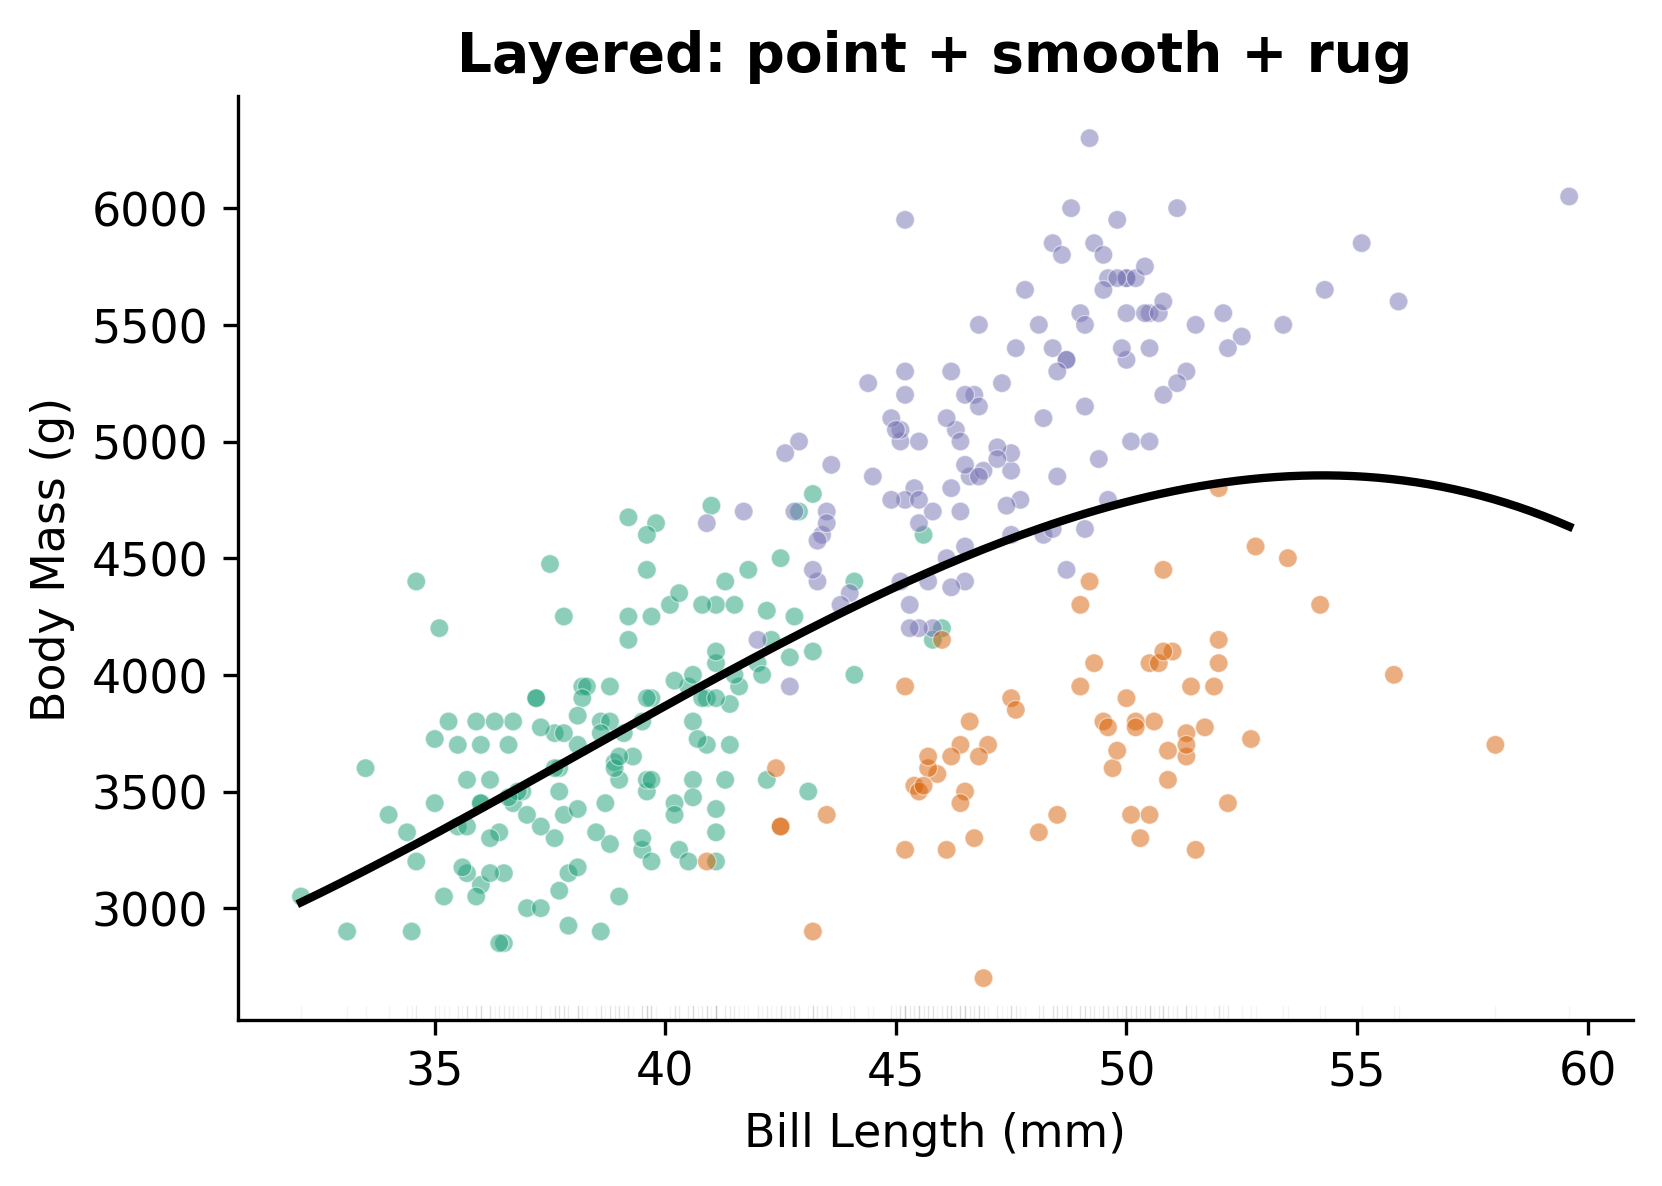
\includegraphics[width=\textwidth]{m1_2_layers.png}
\end{column}
\end{columns}
\end{frame}

% ── 42 ──
\begin{frame}[fragile]{Layering Geoms --- \Python}\smark{42/300}
\begin{columns}[T]
\begin{column}{0.55\textwidth}
\begin{lstlisting}[style=Pystyle]
(ggplot(mpg, aes("displ","hwy"))
 + geom_point(aes(color="class"),
              alpha=0.7)
 + geom_smooth(method="loess",
               color="black")
 + geom_rug(sides="bl",alpha=0.3))
\end{lstlisting}
\scriptref{scripts/m1\_2\_layers.py}
\end{column}
\begin{column}{0.42\textwidth}
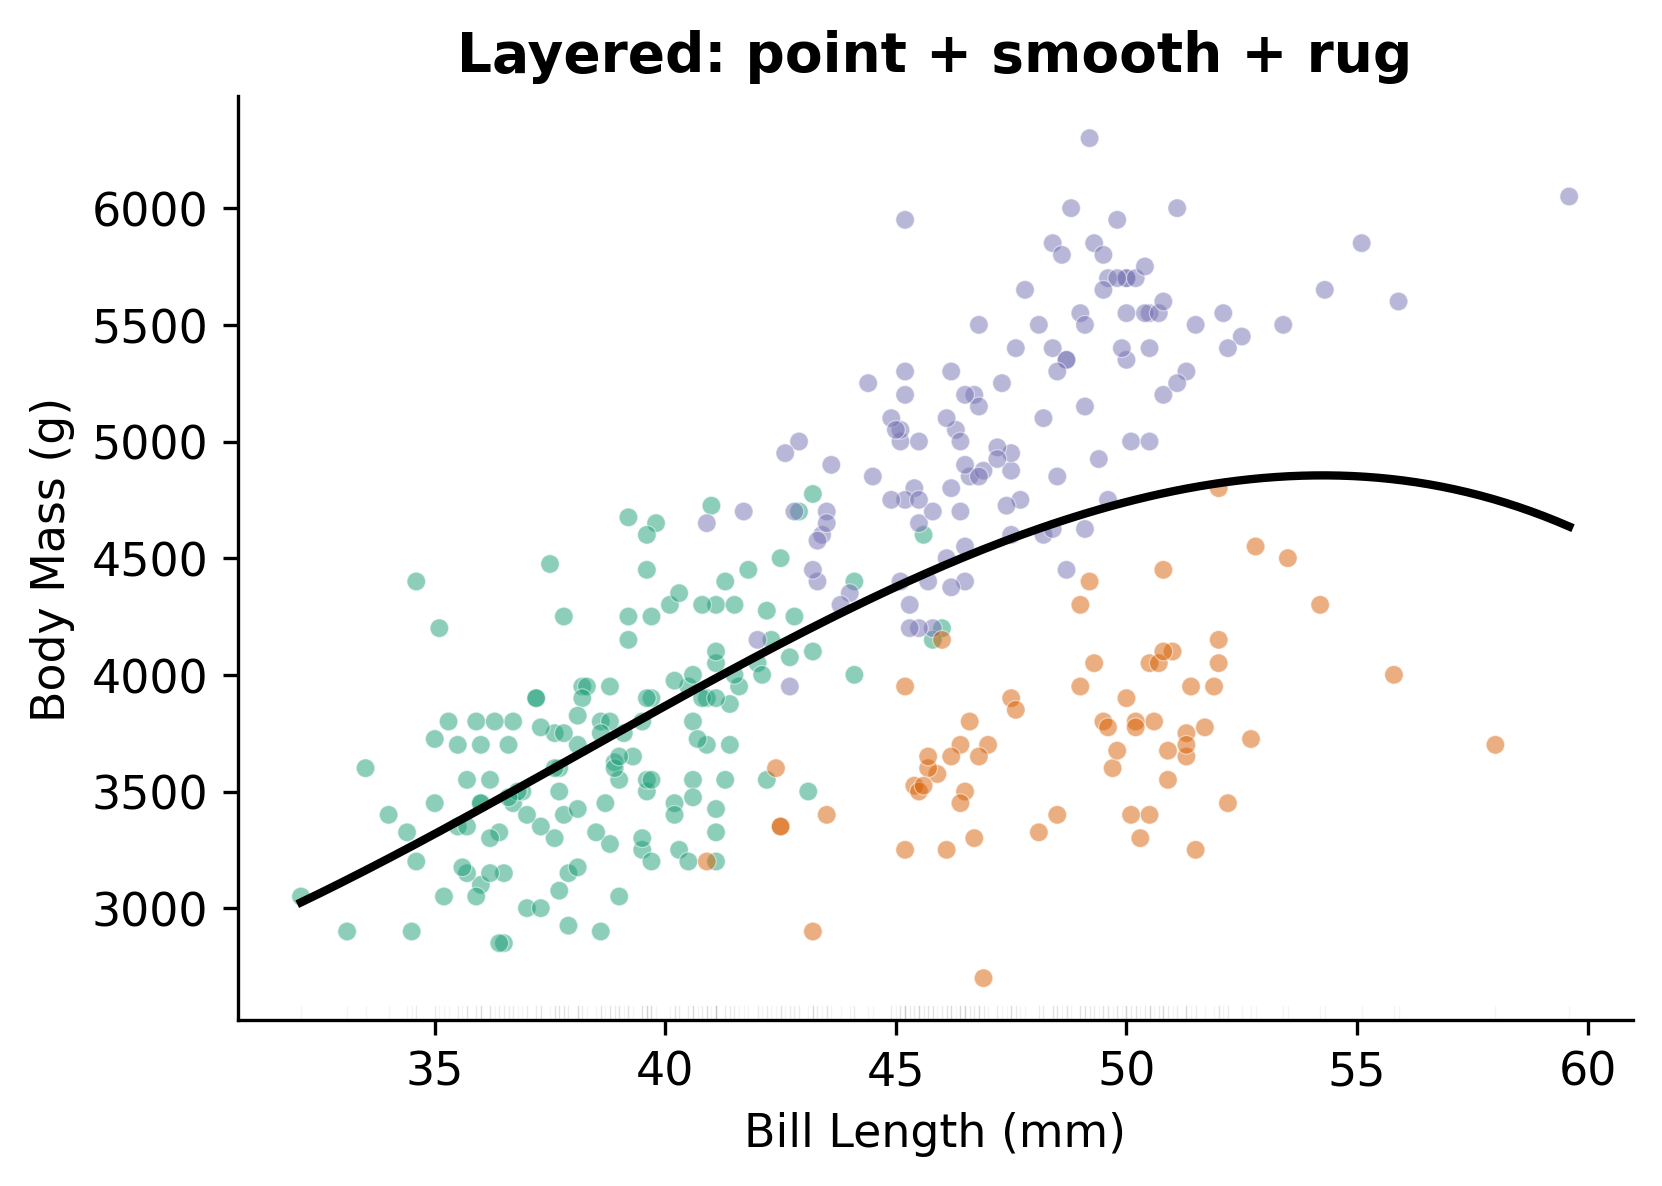
\includegraphics[width=\textwidth]{m1_2_layers.png}
\begin{alertblock}{Pro-Tip}
    \scriptsize Parentheses around the expression for \texttt{+} continuation.
\end{alertblock}
\end{column}
\end{columns}
\end{frame}

% ── 43 ──
\begin{frame}{Component 4: Statistical Transformations}\smark{43/300}
\centering\small
\begin{tabular}{@{}lll@{}}
    \toprule
    \textbf{Geom} & \textbf{Default Stat} & \textbf{Action} \\
    \midrule
    \texttt{geom\_bar}       & \texttt{stat\_count}    & Counts rows \\
    \texttt{geom\_histogram} & \texttt{stat\_bin}      & Bins data \\
    \texttt{geom\_smooth}    & \texttt{stat\_smooth}   & Fits model \\
    \texttt{geom\_point}     & \texttt{stat\_identity} & None \\
    \texttt{geom\_col}       & \texttt{stat\_identity} & None \\
    \bottomrule
\end{tabular}
\end{frame}

% ── 44 ──
\begin{frame}[fragile]{\texttt{geom\_bar} vs.\ \texttt{geom\_col}}\smark{44/300}
\begin{columns}[T]
\begin{column}{0.48\textwidth}
\begin{lstlisting}[style=Rstyle]
# Auto-counts rows per cut
ggplot(diamonds, aes(cut)) +
  geom_bar(fill="#2166AC")
\end{lstlisting}
\scriptsize Categorical column only.
\end{column}
\begin{column}{0.48\textwidth}
\begin{lstlisting}[style=Rstyle]
# Uses pre-computed values
ggplot(df, aes(cut, price)) +
  geom_col(fill="#B2182B")
\end{lstlisting}
\scriptsize Pre-aggregated values.
\end{column}
\end{columns}
\vspace{0.2cm}
\begin{alertblock}{Pro-Tip}
    \scriptsize \texttt{geom\_bar} counts; \texttt{geom\_col} plots. Confusing them = mistake \#2.
\end{alertblock}
\end{frame}

% ── 45 ──
\begin{frame}[fragile]{Stats --- \Python}\smark{45/300}
\begin{columns}[T]
\begin{column}{0.48\textwidth}
\centering\textbf{plotnine}\\[0.1cm]
\begin{lstlisting}[style=Pystyle]
(ggplot(diamonds, aes(x="cut"))
 + geom_bar(fill="#B2182B"))
\end{lstlisting}
\end{column}
\begin{column}{0.48\textwidth}
\centering\textbf{seaborn}\\[0.1cm]
\begin{lstlisting}[style=Pystyle]
sns.countplot(data=diamonds,
              x="cut",
              color="#B2182B")
\end{lstlisting}
\end{column}
\end{columns}
\vspace{0.2cm}
\begin{exampleblock}{Data Insight}
    \scriptsize seaborn hides stats in function names: \texttt{countplot} = geom\_bar + stat\_count.
\end{exampleblock}
\end{frame}

% ── 46 ──
\begin{frame}{Component 5: Scales}\smark{46/300}
\begin{columns}[T]
\begin{column}{0.52\textwidth}
Scales: \textbf{data values} $\to$ \textbf{visual values}
\begin{itemize}
    \item \texttt{scale\_x\_continuous()} --- limits, breaks
    \item \texttt{scale\_color\_brewer()} --- palette
    \item \texttt{scale\_fill\_viridis\_c()} --- uniform
    \item \texttt{scale\_size()} --- range
\end{itemize}
\end{column}
\begin{column}{0.45\textwidth}
\begin{alertblock}{Pro-Tip}
    \scriptsize Pattern: \texttt{scale\_\{aes\}\_\{type\}()}.
\end{alertblock}
\end{column}
\end{columns}
\end{frame}

% ── 47 ──
\begin{frame}[fragile]{Scales --- \Rlang}\smark{47/300}
\begin{columns}[T]
\begin{column}{0.55\textwidth}
\begin{lstlisting}[style=Rstyle]
ggplot(mpg, aes(displ, hwy,
                color=class)) +
  geom_point(size=2) +
  scale_x_continuous(limits=c(1,7),
    breaks=seq(1,7,1)) +
  scale_color_brewer(palette="Set2")
\end{lstlisting}
\end{column}
\begin{column}{0.42\textwidth}
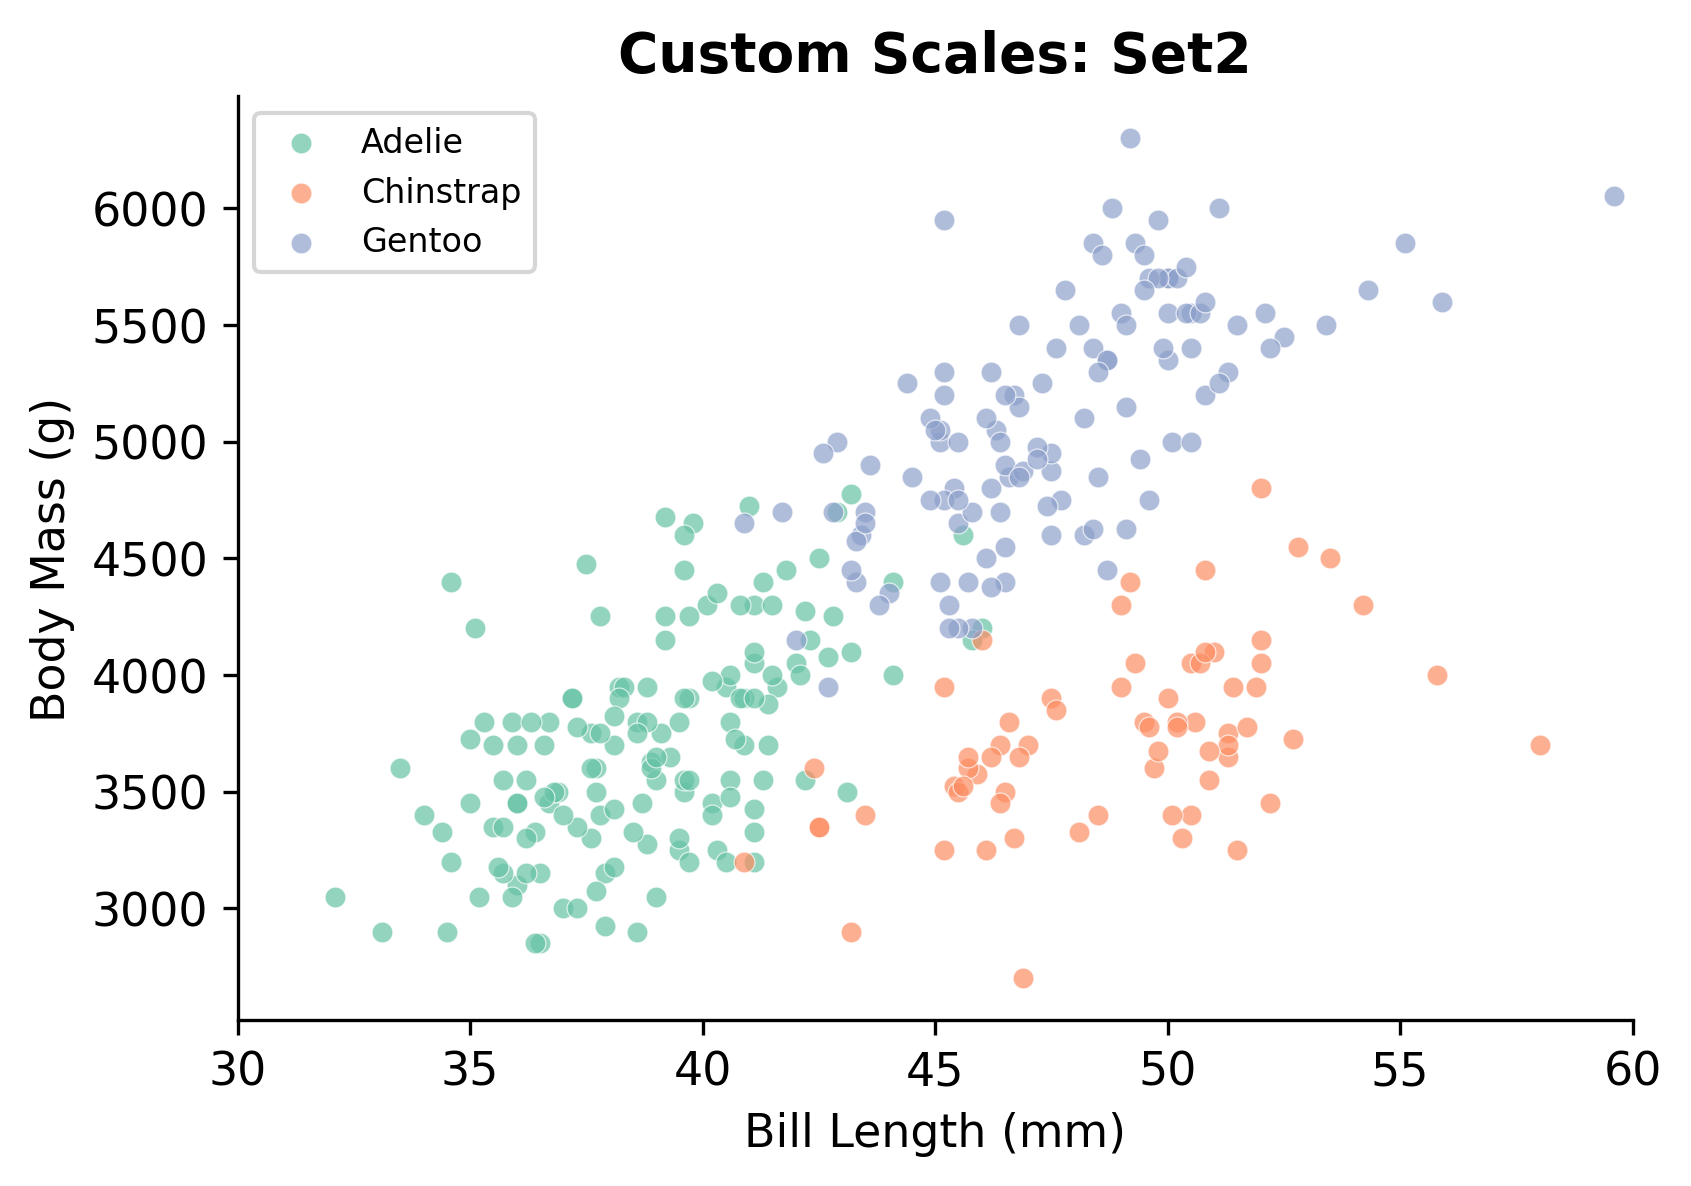
\includegraphics[width=\textwidth]{m1_2_scales.png}
\end{column}
\end{columns}
\end{frame}

% ── 48 ──
\begin{frame}[fragile]{Scales --- \Python}\smark{48/300}
\begin{columns}[T]
\begin{column}{0.55\textwidth}
\begin{lstlisting}[style=Pystyle]
(ggplot(mpg, aes("displ","hwy",
                  color="class"))
 + geom_point(size=2)
 + scale_x_continuous(limits=(1,7))
 + scale_color_brewer(
     type="qual",palette="Set2"))
\end{lstlisting}
\end{column}
\begin{column}{0.42\textwidth}
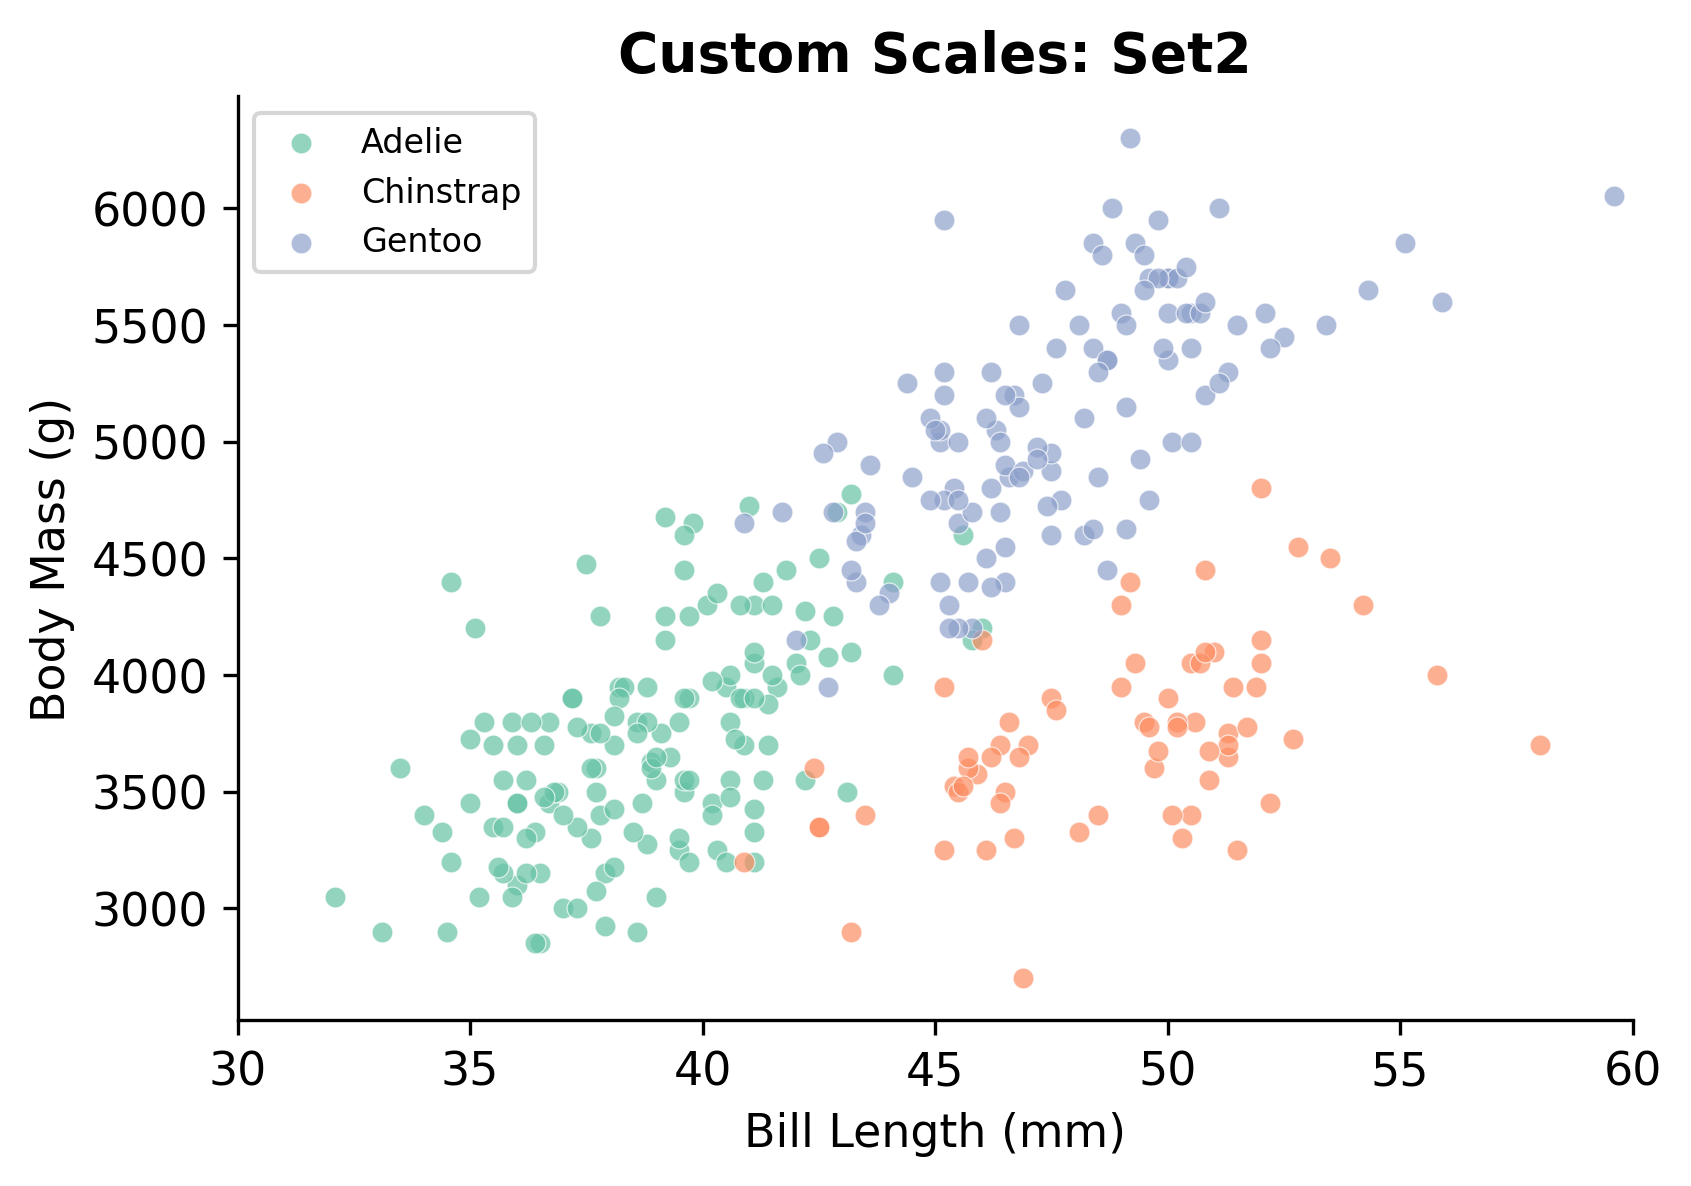
\includegraphics[width=\textwidth]{m1_2_scales.png}
\end{column}
\end{columns}
\end{frame}

% ── 49 ──
\begin{frame}{Component 6: Coordinates}\smark{49/300}
\centering\small
\begin{tabular}{@{}lll@{}}
    \toprule
    \textbf{Coord} & \textbf{Use} & \textbf{Note} \\
    \midrule
    \texttt{coord\_cartesian} & Default    & Zoom without data loss \\
    \texttt{coord\_flip}      & Swap axes  & Long labels \\
    \texttt{coord\_polar}     & Polar      & Pie, wind roses \\
    \texttt{coord\_sf}        & Maps       & Module 6 \\
    \bottomrule
\end{tabular}
\vspace{0.3cm}
\begin{alertblock}{Pro-Tip}
    \scriptsize \texttt{coord\_cartesian(ylim=...)} = viewport zoom. \texttt{scale\_y(limits=...)} = data filter. Different!
\end{alertblock}
\end{frame}

% ── 50 ──
\begin{frame}[fragile]{Zoom Trap}\smark{50/300}
\begin{columns}[T]
\begin{column}{0.48\textwidth}
\centering\textbf{Safe}\\[0.1cm]
\begin{lstlisting}[style=Rstyle]
ggplot(mpg, aes(displ,hwy)) +
  geom_smooth() +
  coord_cartesian(ylim=c(20,40))
\end{lstlisting}
\scriptsize Smoother on \textbf{all} data.
\end{column}
\begin{column}{0.48\textwidth}
\centering\textbf{Dangerous}\\[0.1cm]
\begin{lstlisting}[style=Rstyle]
ggplot(mpg, aes(displ,hwy)) +
  geom_smooth() +
  scale_y_continuous(
    limits=c(20,40))
\end{lstlisting}
\scriptsize Data \textbf{dropped} first.
\end{column}
\end{columns}
\end{frame}

% ── 51 ──
\begin{frame}[fragile]{Coords --- \Python}\smark{51/300}
\begin{columns}[T]
\begin{column}{0.48\textwidth}
\centering\textbf{plotnine}\\[0.1cm]
\begin{lstlisting}[style=Pystyle]
(ggplot(mpg, aes("displ","hwy"))
 + geom_smooth()
 + coord_cartesian(ylim=(20,40)))
\end{lstlisting}
\end{column}
\begin{column}{0.48\textwidth}
\centering\textbf{matplotlib}\\[0.1cm]
\begin{lstlisting}[style=Pystyle]
ax.set_ylim(20, 40)  # viewport
\end{lstlisting}
\scriptsize \texttt{set\_ylim} = viewport (safe).
\end{column}
\end{columns}
\end{frame}

% ── 52 ──
\begin{frame}{Component 7: Themes \& Facets}\smark{52/300}
\begin{columns}[T]
\begin{column}{0.48\textwidth}
\textbf{Themes} (non-data):
\begin{itemize}
    \item Fonts, background, gridlines
    \item Legend position
    \item Axis ticks, borders
\end{itemize}
\end{column}
\begin{column}{0.48\textwidth}
\textbf{Facets} (panels):
\begin{itemize}
    \item \texttt{facet\_wrap(\textasciitilde var)}
    \item \texttt{facet\_grid(row\textasciitilde col)}
    \item Free or shared scales
\end{itemize}
\end{column}
\end{columns}
\end{frame}

% ── 53 ──
\begin{frame}[fragile]{Full Pipeline --- \Rlang}\smark{53/300}
\begin{columns}[T]
\begin{column}{0.55\textwidth}
\begin{lstlisting}[style=Rstyle]
ggplot(penguins,           # 1 Data
  aes(bill_length_mm,      # 2 Aes
      body_mass_g,
      color=species)) +
  geom_point(alpha=0.7) +  # 3 Geom
  geom_smooth(method="lm", # 4 Stat
              se=FALSE) +
  scale_color_brewer(       # 5 Scale
    palette="Dark2") +
  facet_wrap(~island) +     # 7 Facet
  theme_minimal()           # 7 Theme
\end{lstlisting}
\scriptref{scripts/m1\_2\_grammar\_full.R}
\end{column}
\begin{column}{0.42\textwidth}
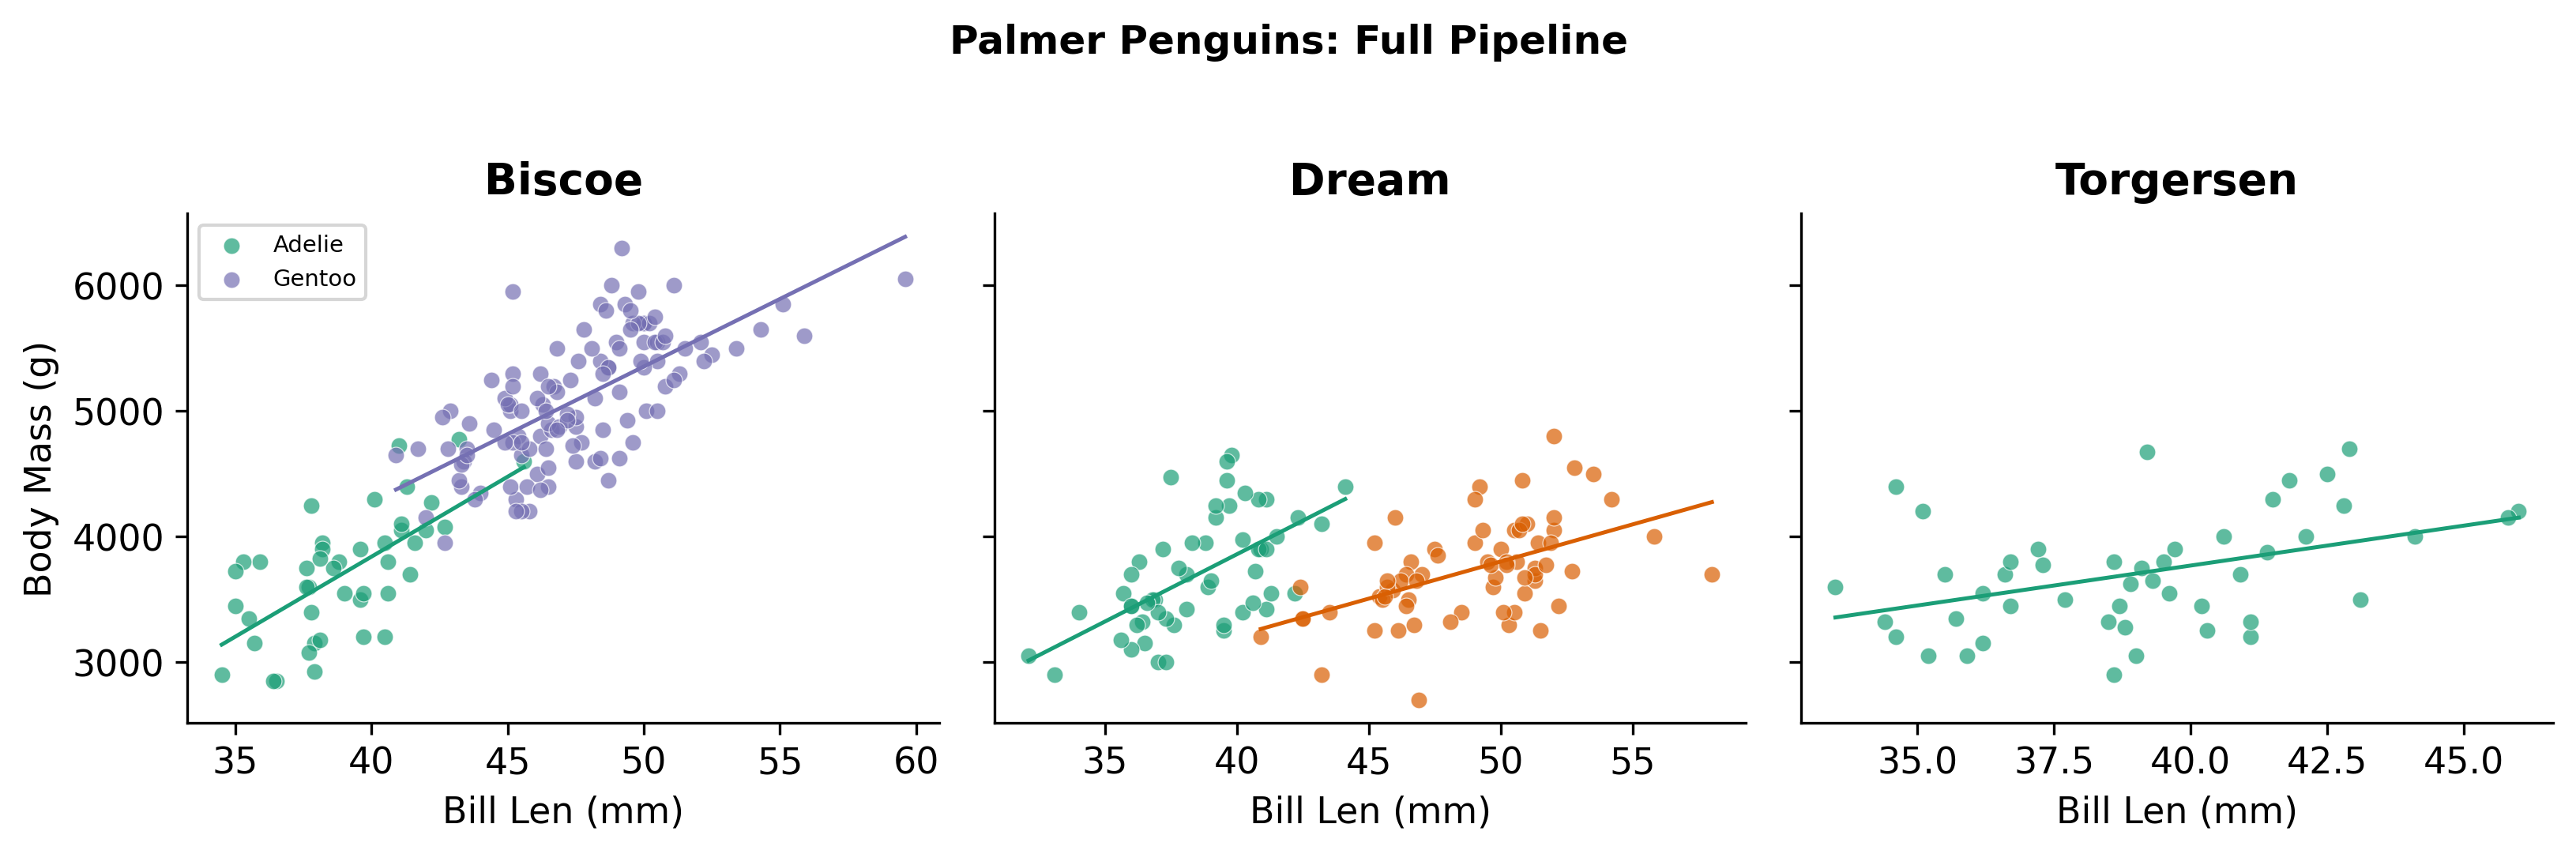
\includegraphics[width=\textwidth]{m1_2_pipeline.png}
\begin{exampleblock}{Data Insight}
    \scriptsize All 7 components in one block. This is the mental model for every plot.
\end{exampleblock}
\end{column}
\end{columns}
\end{frame}

% ── 54 ──
\begin{frame}[fragile]{Full Pipeline --- \Python}\smark{54/300}
\begin{columns}[T]
\begin{column}{0.55\textwidth}
\begin{lstlisting}[style=Pystyle]
(ggplot(penguins,           # 1
   aes("bill_length_mm",   # 2
       "body_mass_g",
       color="species"))
 + geom_point(alpha=0.7)   # 3
 + geom_smooth(method="lm",# 4
               se=False)
 + scale_color_brewer(      # 5
     type="qual",palette="Dark2")
 + facet_wrap("~island")    # 7
 + theme_minimal())
\end{lstlisting}
\scriptref{scripts/m1\_2\_grammar\_full.py}
\end{column}
\begin{column}{0.42\textwidth}
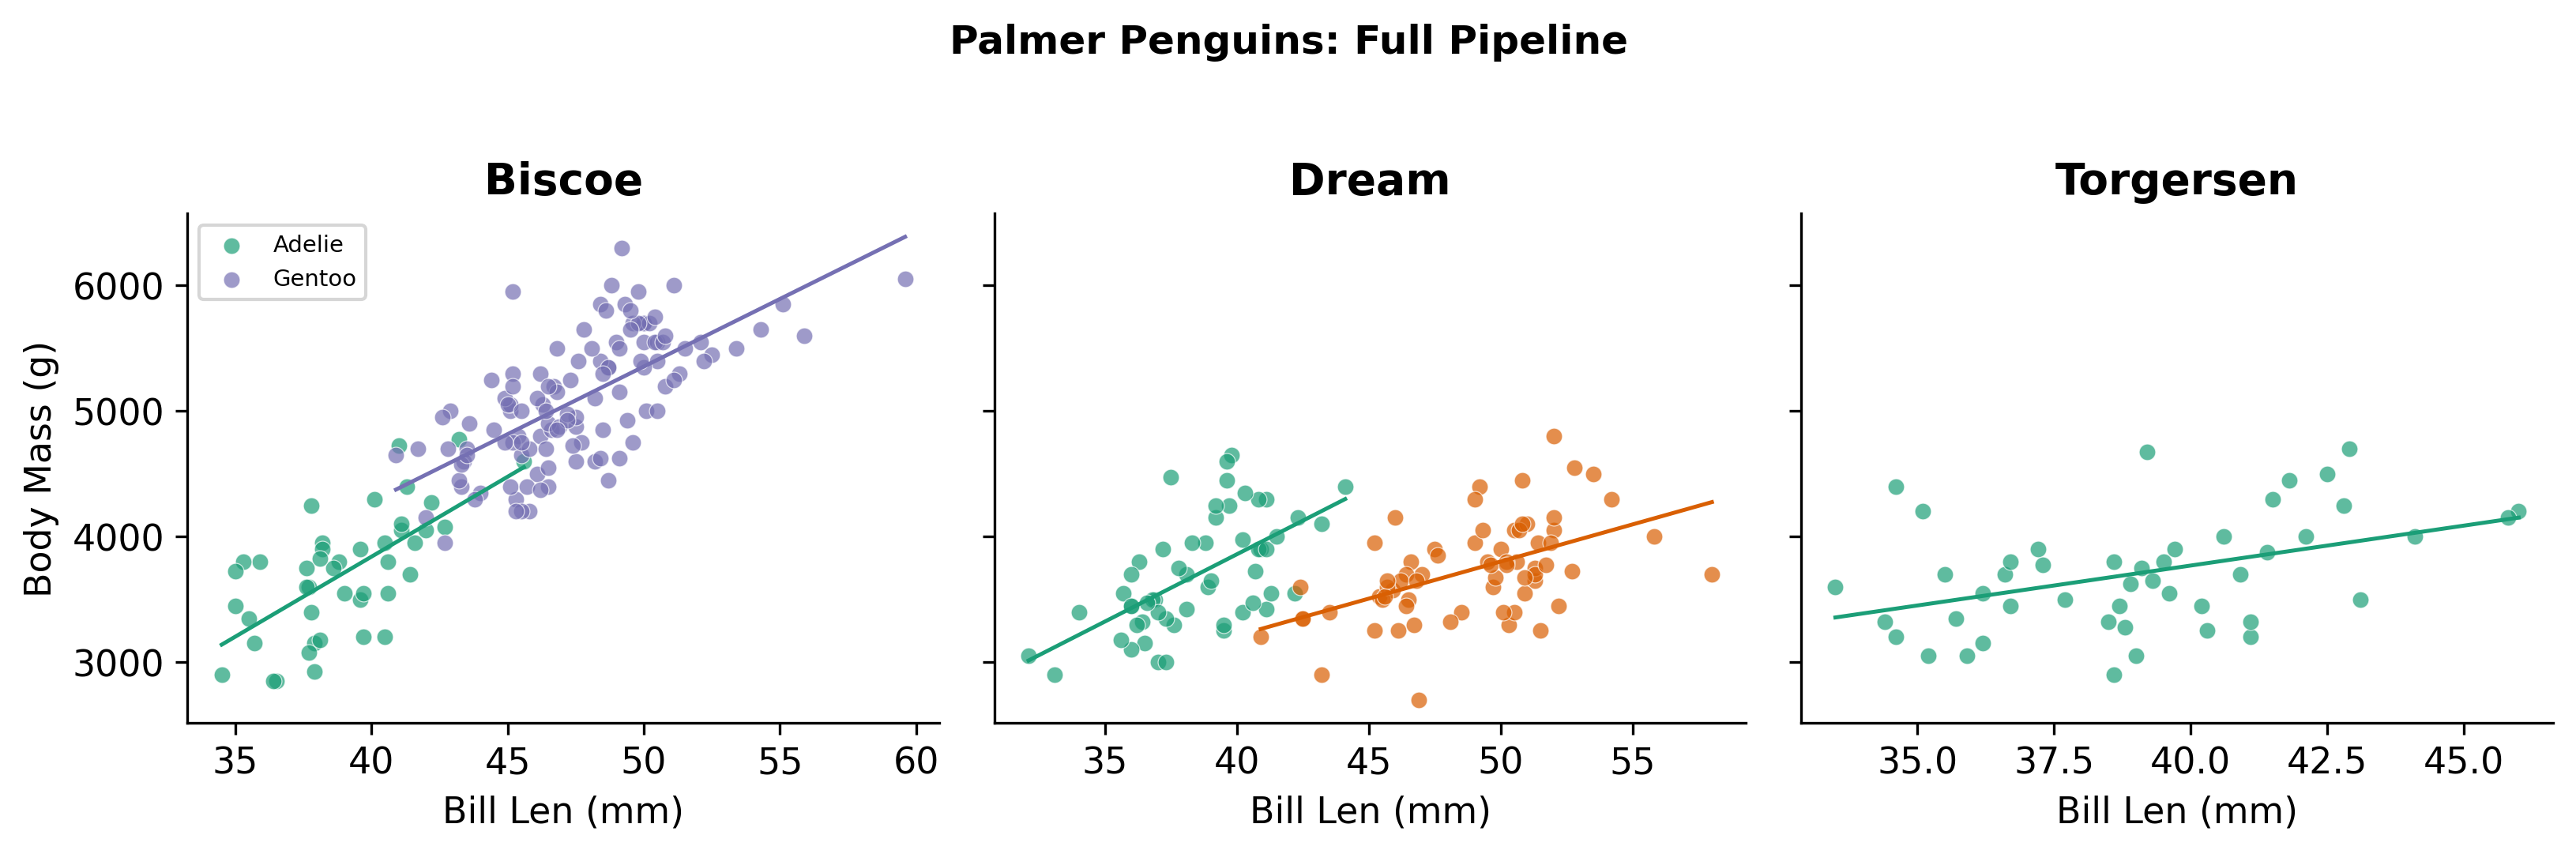
\includegraphics[width=\textwidth]{m1_2_pipeline.png}
\begin{alertblock}{Pro-Tip}
    \scriptsize R and Python: \textbf{line-for-line identical}. Learn one, transfer.
\end{alertblock}
\end{column}
\end{columns}
\end{frame}

% ── 55 ──
\begin{frame}[fragile]{Same Plot --- \texttt{matplotlib} (no grammar)}\smark{55/300}
\begin{columns}[T]
\begin{column}{0.55\textwidth}
\begin{lstlisting}[style=Pystyle]
# 35+ lines required:
# manual color dict per species
# loop over islands (subplots)
# nested loop over species
# manual OLS per group
# manual legend, labels, titles
# See full script for comparison.
\end{lstlisting}
\scriptref{scripts/m1\_2\_mpl\_comparison.py}
\end{column}
\begin{column}{0.42\textwidth}
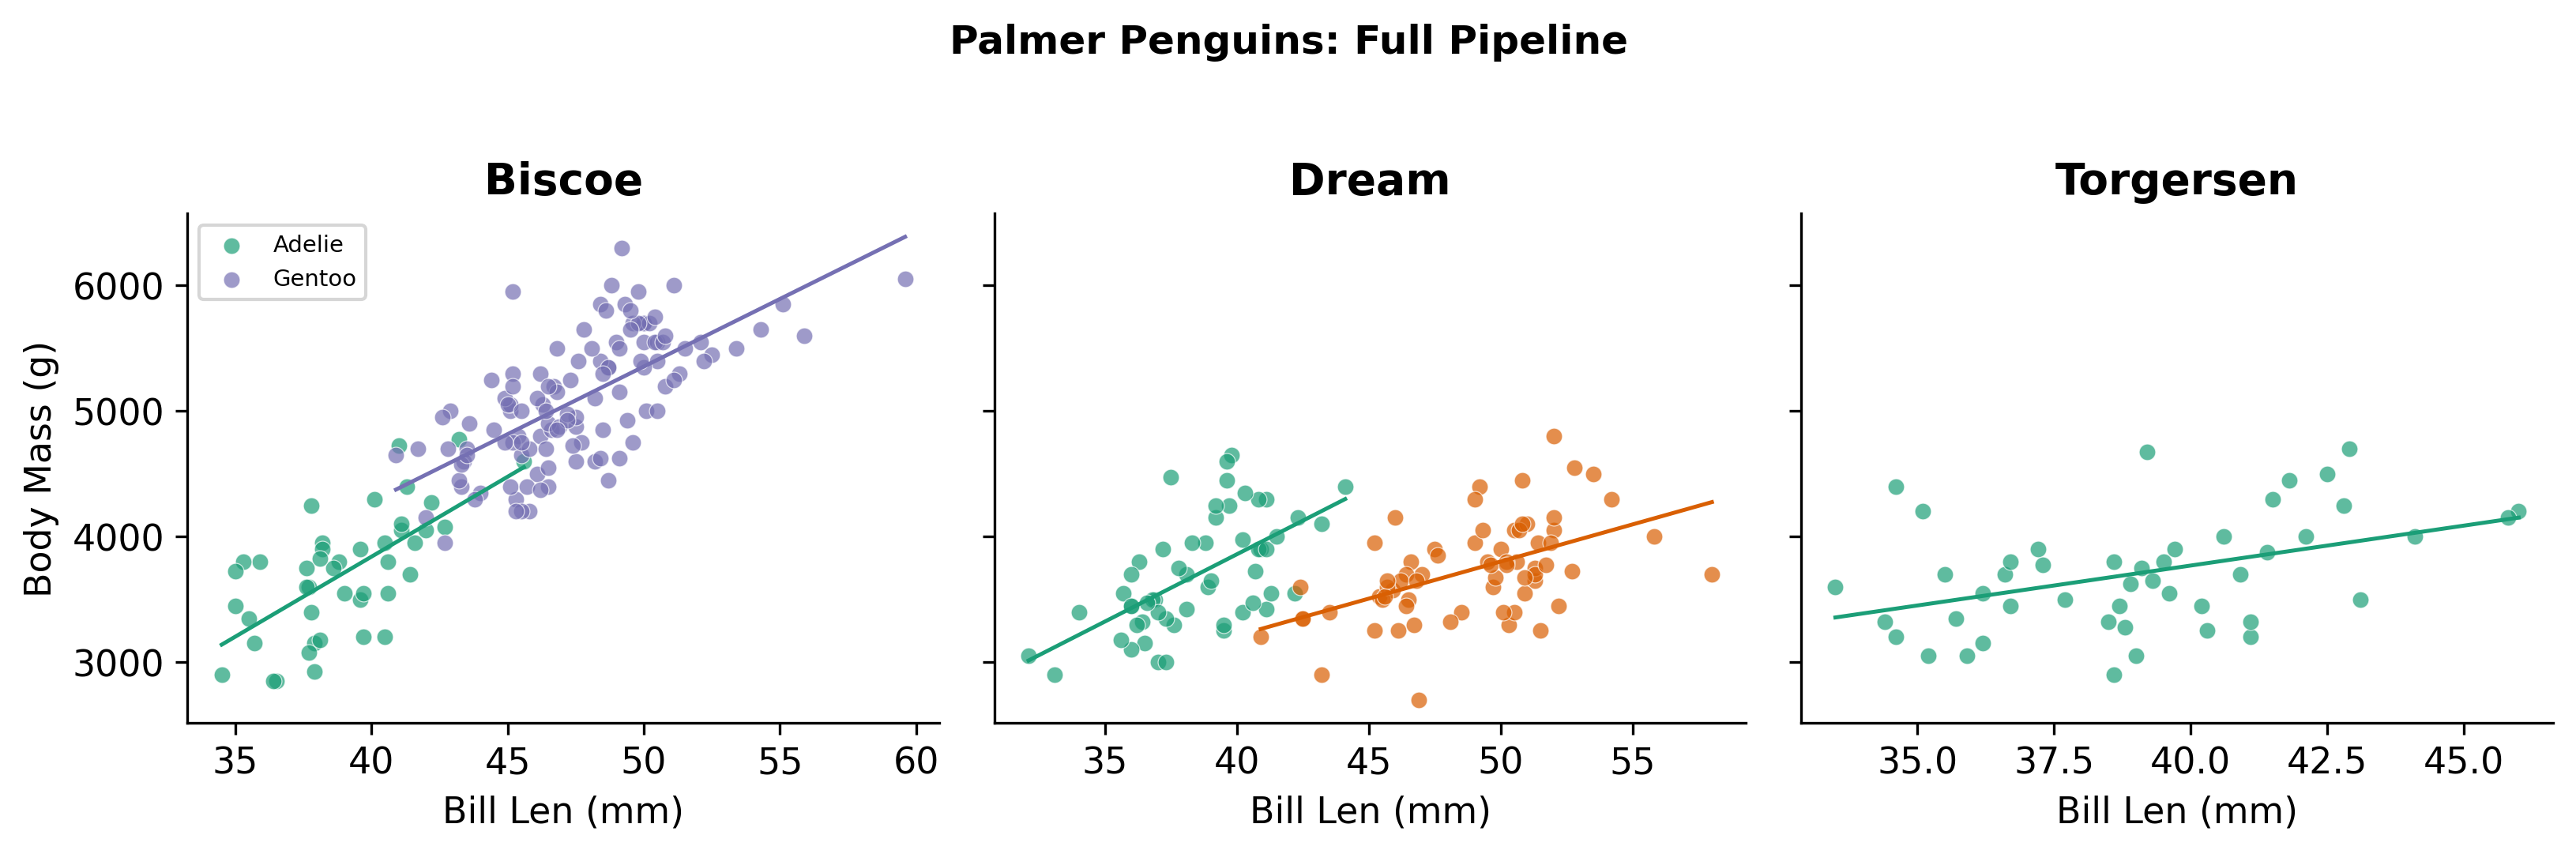
\includegraphics[width=\textwidth]{m1_2_pipeline.png}
\begin{alertblock}{Pro-Tip}
    \scriptsize 35 lines of matplotlib vs.\ 12 lines of plotnine for the \emph{same} result.
\end{alertblock}
\end{column}
\end{columns}
\end{frame}

% ── 56 ──
\begin{frame}[fragile]{Grammar as Pseudocode}\smark{56/300}
\centering
\begin{lstlisting}[basicstyle=\ttfamily\small,frame=none,
    backgroundcolor=\color{backcolour},xleftmargin=1cm]
PLOT =
  DATA(source)
  + AESTHETICS(x, y, color, size)
  + GEOMETRY(point | line | bar)
  + STATISTICS(identity | bin | smooth)
  + SCALES(limits, palette)
  + COORDINATES(cartesian | polar)
  + FACETS(wrap | grid)
  + THEME(fonts, background)
\end{lstlisting}
\vspace{0.2cm}
\begin{exampleblock}{Data Insight}
    \scriptsize Language-agnostic. R, Python, Julia, JS --- same mental model.
\end{exampleblock}
\end{frame}

% ── 57 ──
\begin{frame}{Ecosystem Comparison}\smark{57/300}
\centering\scriptsize
\begin{tabular}{@{}llll@{}}
    \toprule
    \textbf{Feature} & \textbf{ggplot2} & \textbf{plotnine} & \textbf{matplotlib} \\
    \midrule
    Paradigm      & Declarative & Declarative  & Imperative \\
    Grammar       & Yes         & Yes (port)   & No \\
    Faceting      & Built-in    & Built-in     & Manual \\
    Stat layers   & Implicit    & Implicit     & Manual \\
    Themes        & \texttt{theme()} & \texttt{theme()} & \texttt{rcParams} \\
    Extensions    & 200+ pkgs   & Growing      & Vast \\
    \bottomrule
\end{tabular}
\end{frame}

% ── 58 ──
\begin{frame}[fragile]{The \texttt{+} Operator}\smark{58/300}
\begin{columns}[T]
\begin{column}{0.48\textwidth}
\begin{lstlisting}[style=Rstyle]
p <- ggplot(mpg, aes(displ,hwy))
p <- p + geom_point()
p <- p + geom_smooth()
p  # render
\end{lstlisting}
\end{column}
\begin{column}{0.48\textwidth}
\begin{lstlisting}[style=Pystyle]
p = (ggplot(mpg,
       aes("displ","hwy"))
     + geom_point())
p = p + geom_smooth()
p.draw()
\end{lstlisting}
\end{column}
\end{columns}
\vspace{0.2cm}
\begin{exampleblock}{Data Insight}
    \scriptsize \texttt{+} = \textbf{layer composition}, not addition.
\end{exampleblock}
\end{frame}

% ── 59 ──
\begin{frame}{Module 1.2 --- Takeaways}\smark{59/300}
\begin{enumerate}
    \item \textbf{Grammar $\neq$ taxonomy.} data + aes + geom + stat + scale + coord + theme.
    \item \textbf{Tidy data first.} One variable/column, one observation/row.
    \item \textbf{Mapping vs.\ setting.} Inside \texttt{aes()} = data-driven.
    \item \textbf{Every geom has an implicit stat.} Know defaults.
    \item \textbf{ggplot2 $\approx$ plotnine.} Learn one, transfer instantly.
\end{enumerate}
\end{frame}

% ── 60 ──
\begin{frame}{}\smark{60/300}
\centering\vspace{1.5cm}
{\Large\textbf{Module 1.2 Complete}}\\[0.5cm]
You have the \textbf{theoretical framework} for every visualization in this course.\\[0.5cm]
\textbf{Next:} Module 1.3 --- \texttt{geom\_point}, \texttt{geom\_col}, \texttt{geom\_line} from raw data.
\end{frame}

% ═══════════════════════════════════════════════════════
%  MODULE 1.3 — Your First Plots: Scatter, Bar, Line
% ═══════════════════════════════════════════════════════
\section{Module 1.3 --- Your First Plots: Scatter, Bar, Line}

% ── 61 ──
\begin{frame}{Module 1.3 --- Roadmap}\smark{61/300}
\begin{enumerate}
    \item The scatter plot: \texttt{geom\_point()}
    \item Mapping 3rd and 4th variables (color, size, shape)
    \item Overplotting: diagnosis and four remedies
    \item The bar chart: \texttt{geom\_col()} and sorting
    \item Position adjustments: stack, dodge, fill, jitter
    \item The line chart: \texttt{geom\_line()} and \texttt{geom\_step()}
    \item Missing data and line gaps
    \item Choosing scatter vs.\ bar vs.\ line
\end{enumerate}
\end{frame}

% ── 62 ──
\begin{frame}{The Scatter Plot: When and Why}
\smark{62/300}
\begin{columns}[T]
\begin{column}{0.50\textwidth}
\begin{itemize}
    \item Shows relationship between two \textbf{continuous} variables
    \item Reveals correlation, clusters, outliers, non-linearity
    \item The most information-dense 2D chart (Wilkinson, 2005)
    \item Default starting point for any bivariate EDA
\end{itemize}
\end{column}
\begin{column}{0.47\textwidth}
\begin{exampleblock}{Data Insight}
    \scriptsize A scatter plot maps both $x$ and $y$ to \textbf{position on a common scale} --- the highest-ranked encoding (Cleveland \& McGill, 1984).
\end{exampleblock}
\vspace{0.2cm}
\begin{alertblock}{Pro-Tip}
    \scriptsize Not for categorical $x$ --- use \texttt{geom\_jitter()} or \texttt{geom\_boxplot()} instead.
\end{alertblock}
\end{column}
\end{columns}
\end{frame}

% ── 63 ──
\begin{frame}[fragile]{Basic Scatter --- \Rlang}\smark{63/300}
\begin{columns}[T]
\begin{column}{0.55\textwidth}
\begin{lstlisting}[style=Rstyle]
library(palmerpenguins)

ggplot(penguins,
  aes(x = bill_length_mm,
      y = body_mass_g)) +
  geom_point(color = "#2166AC",
             alpha = 0.7,
             size = 2) +
  labs(x = "Bill Length (mm)",
       y = "Body Mass (g)") +
  theme_minimal()
\end{lstlisting}
\scriptref{scripts/m1\_3\_scatter\_basic.R}
\end{column}
\begin{column}{0.42\textwidth}
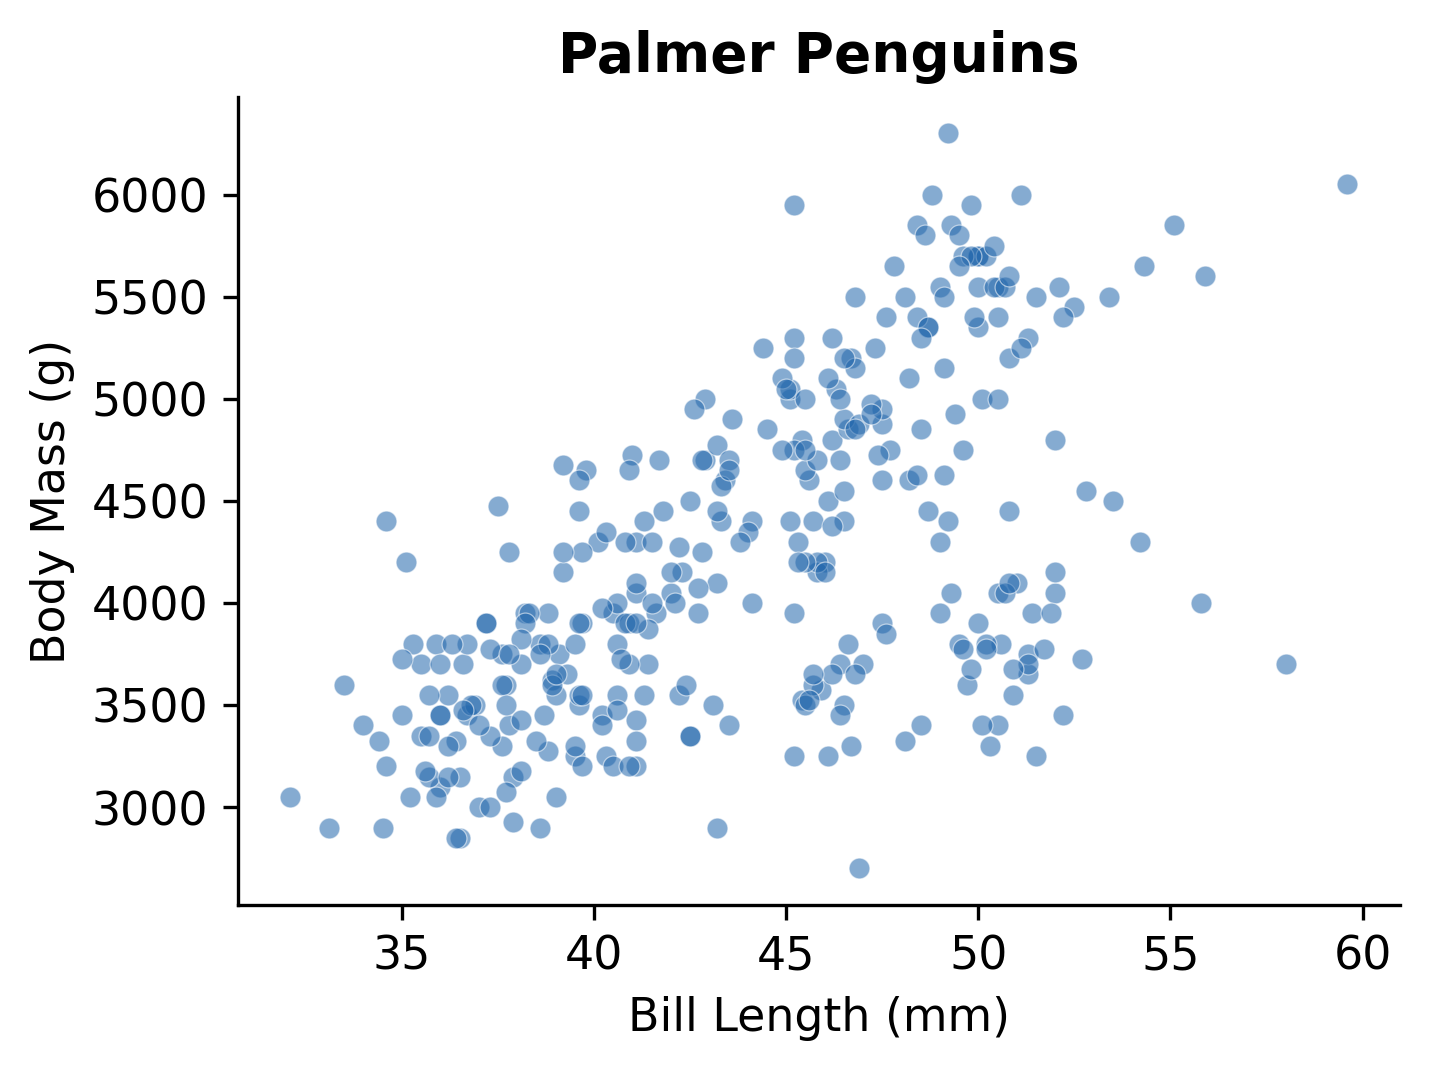
\includegraphics[width=\textwidth]{m1_3_scatter_basic.png}
\begin{exampleblock}{Data Insight}
    \scriptsize Positive trend visible immediately. A few outliers at low bill length / high mass.
\end{exampleblock}
\end{column}
\end{columns}
\end{frame}

% ── 64 ──
\begin{frame}[fragile]{Basic Scatter --- \Python}\smark{64/300}
\begin{columns}[T]
\begin{column}{0.55\textwidth}
\begin{lstlisting}[style=Pystyle]
from plotnine import *
import palmerpenguins as pp
penguins = pp.load_penguins()

(ggplot(penguins,
   aes("bill_length_mm",
       "body_mass_g"))
 + geom_point(color="#B2182B",
              alpha=0.7, size=2)
 + labs(x="Bill Length (mm)",
        y="Body Mass (g)")
 + theme_minimal())
\end{lstlisting}
\scriptref{scripts/m1\_3\_scatter\_basic.py}
\end{column}
\begin{column}{0.42\textwidth}
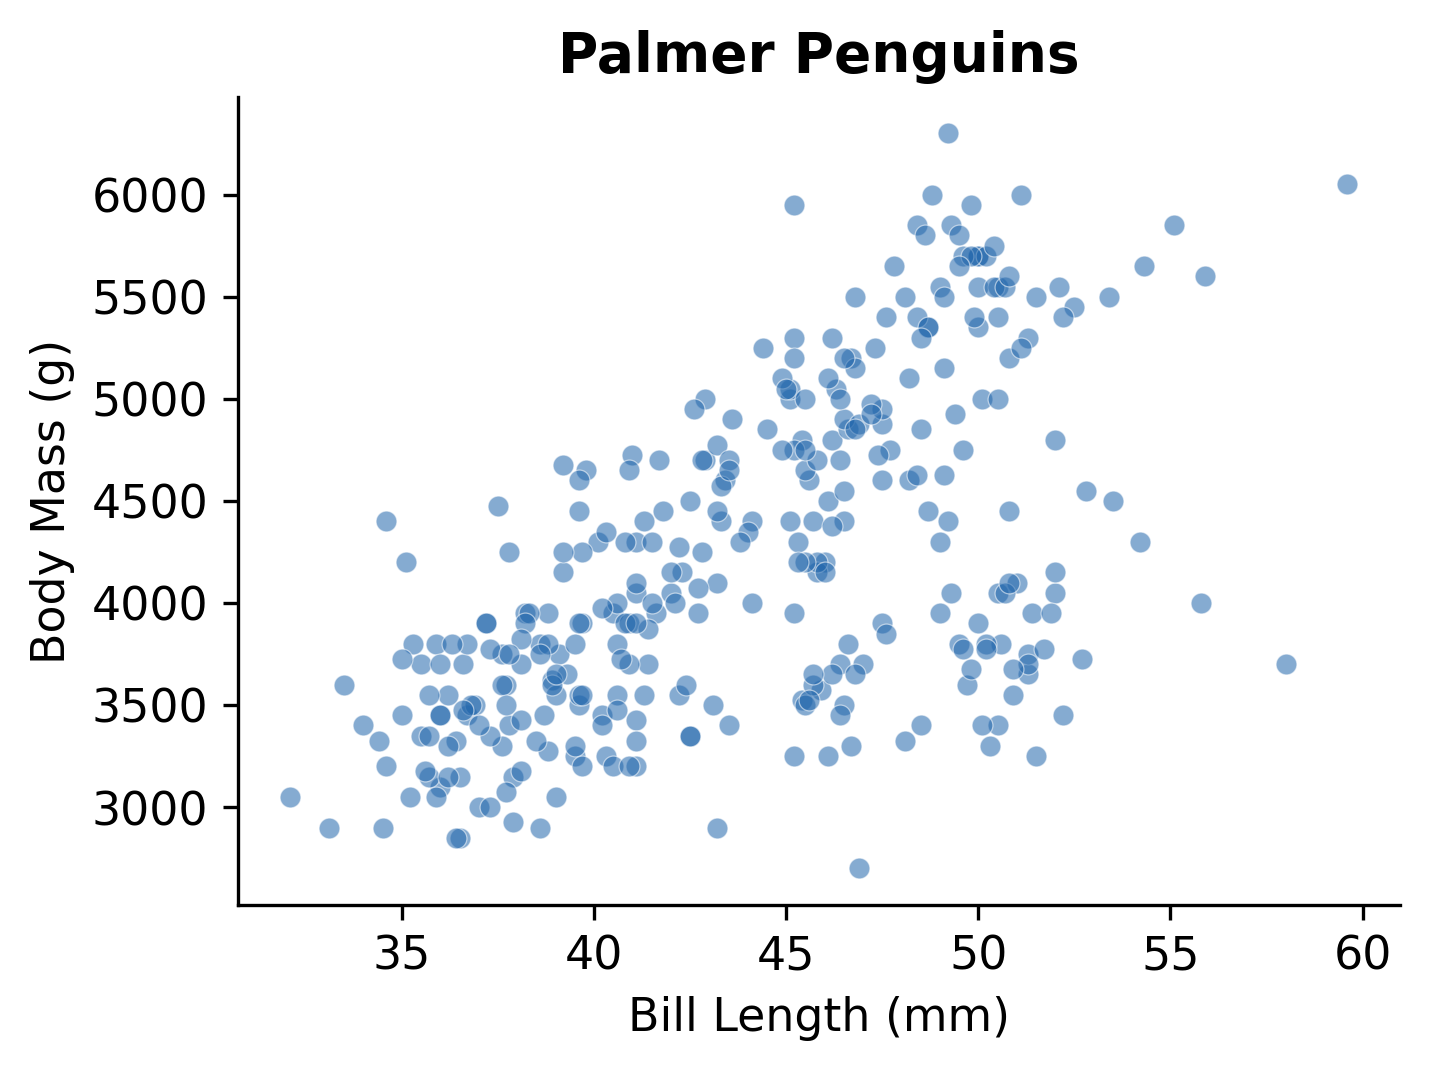
\includegraphics[width=\textwidth]{m1_3_scatter_basic.png}
\begin{alertblock}{Pro-Tip}
    \scriptsize \texttt{alpha} controls transparency (0--1). Start at 0.7; reduce if overplotting appears.
\end{alertblock}
\end{column}
\end{columns}
\end{frame}

% ── 65 ──
\begin{frame}{Adding a Third Variable: Color}
\smark{65/300}
\begin{columns}[T]
\begin{column}{0.50\textwidth}
\begin{itemize}
    \item Map a \textbf{categorical} variable to \texttt{color}
    \item Each group gets a distinct hue
    \item Legend is generated automatically
    \item Reveals group-level patterns hidden in pooled scatter
\end{itemize}
\end{column}
\begin{column}{0.47\textwidth}
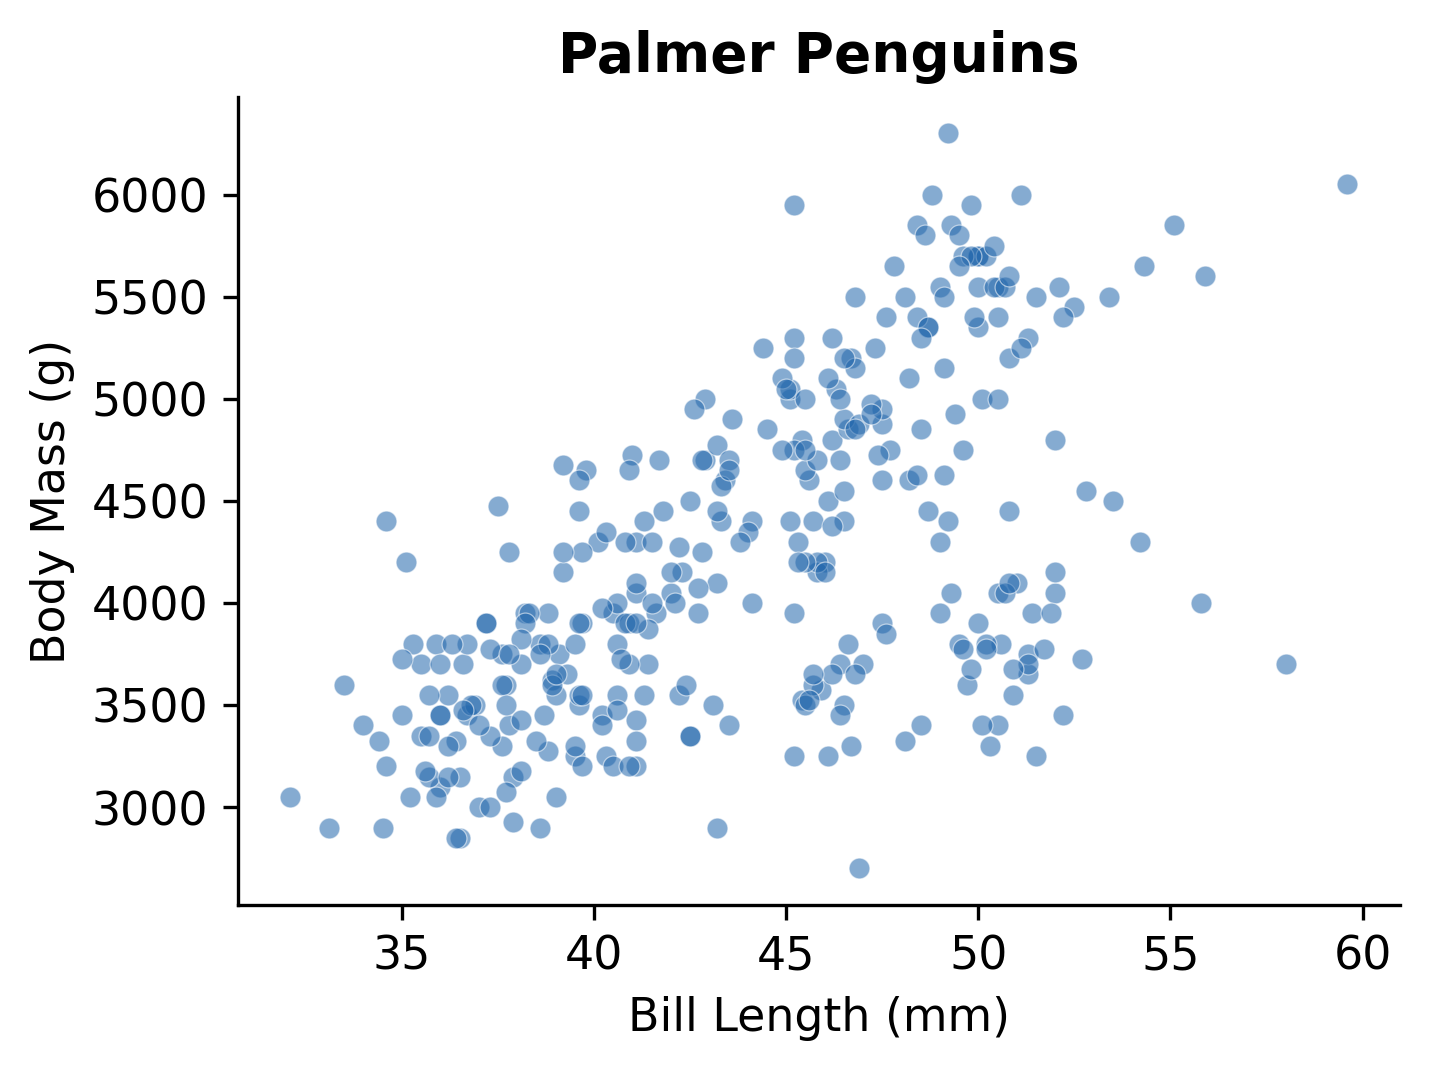
\includegraphics[width=\textwidth]{m1_3_scatter_basic.png}
\begin{exampleblock}{Data Insight}
    \scriptsize Three species form distinct clusters --- invisible in the monochrome version on slide 63.
\end{exampleblock}
\end{column}
\end{columns}
\end{frame}

% ── 66 ──
\begin{frame}[fragile]{Color Mapping --- \Rlang}\smark{66/300}
\begin{columns}[T]
\begin{column}{0.55\textwidth}
\begin{lstlisting}[style=Rstyle]
ggplot(penguins,
  aes(x = bill_length_mm,
      y = body_mass_g,
      color = species)) +
  geom_point(alpha = 0.7) +
  scale_color_brewer(
    palette = "Dark2") +
  theme_minimal()
\end{lstlisting}
\end{column}
\begin{column}{0.42\textwidth}
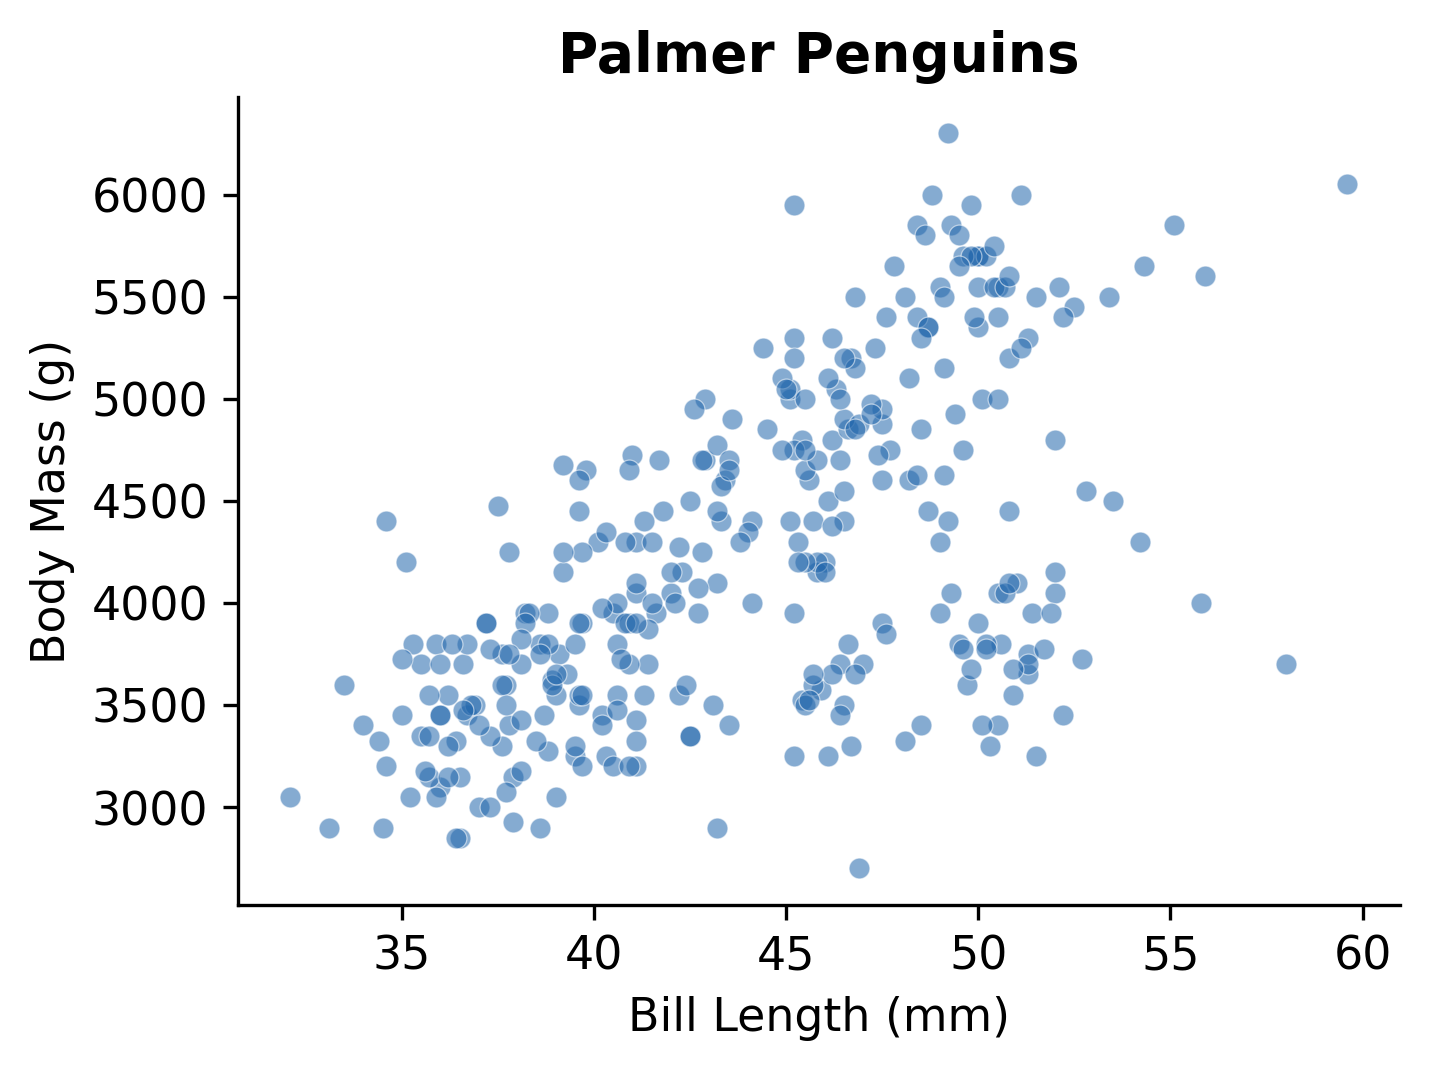
\includegraphics[width=\textwidth]{m1_3_scatter_basic.png}
\begin{alertblock}{Pro-Tip}
    \scriptsize \texttt{scale\_color\_brewer()} for categorical (qualitative palettes). \texttt{scale\_color\_viridis\_c()} for continuous.
\end{alertblock}
\end{column}
\end{columns}
\end{frame}

% ── 67 ──
\begin{frame}[fragile]{Color Mapping --- \Python}\smark{67/300}
\begin{columns}[T]
\begin{column}{0.55\textwidth}
\begin{lstlisting}[style=Pystyle]
(ggplot(penguins,
   aes("bill_length_mm",
       "body_mass_g",
       color="species"))
 + geom_point(alpha=0.7)
 + scale_color_brewer(
     type="qual", palette="Dark2")
 + theme_minimal())
\end{lstlisting}
\end{column}
\begin{column}{0.42\textwidth}
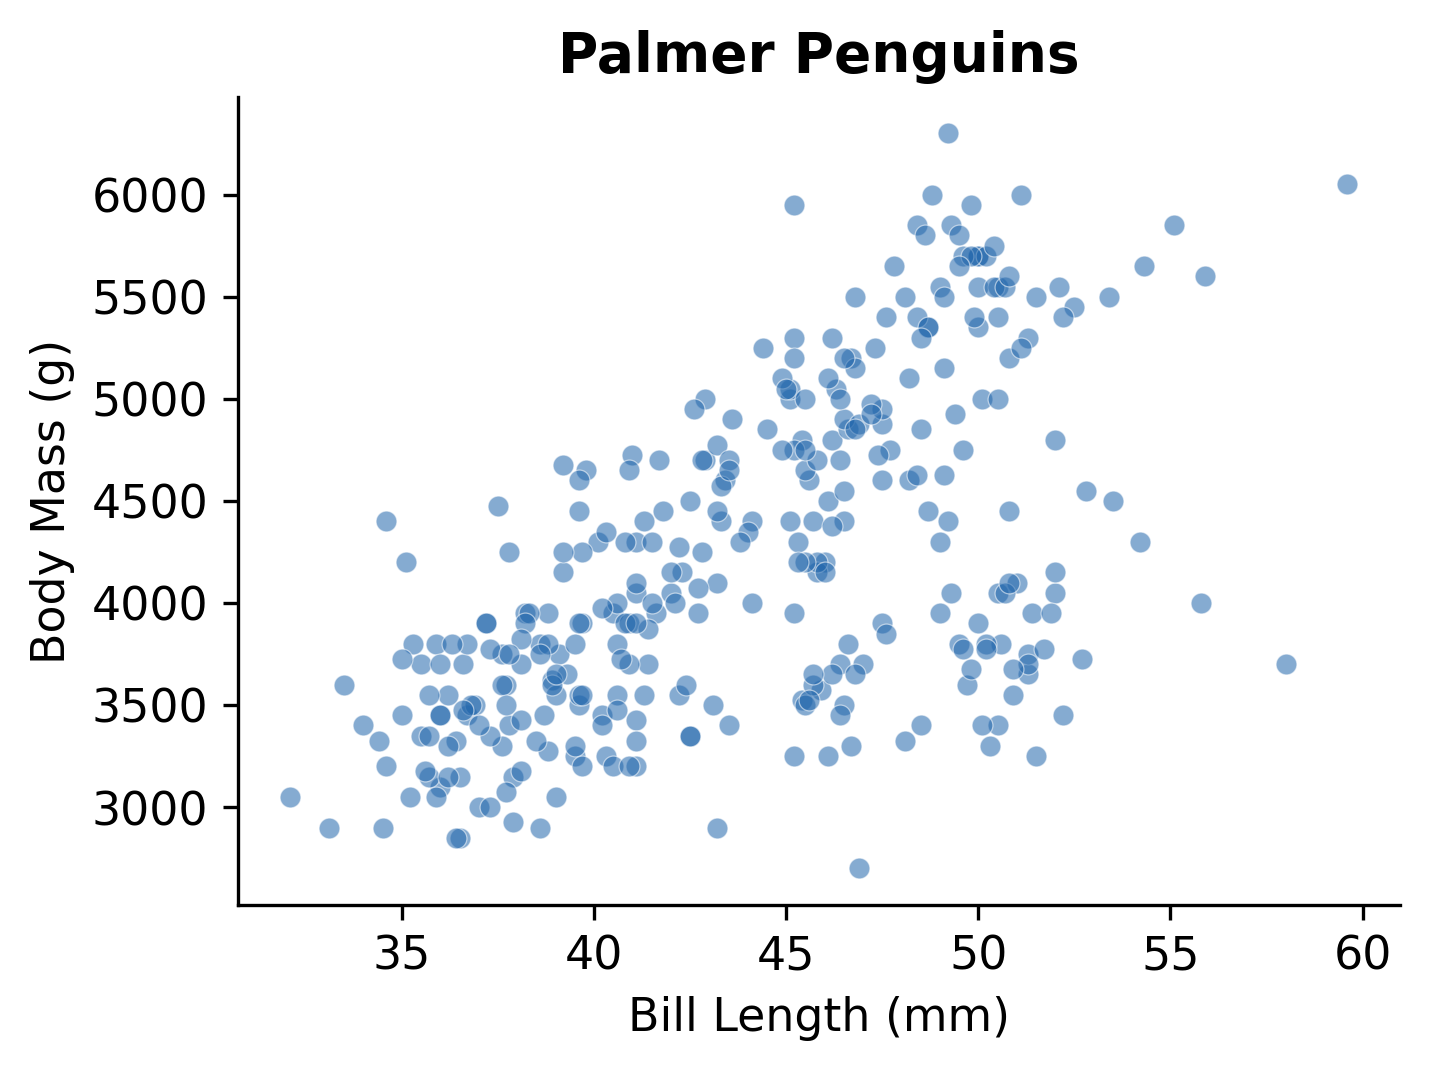
\includegraphics[width=\textwidth]{m1_3_scatter_basic.png}
\end{column}
\end{columns}
\end{frame}

% ── 68 ──
\begin{frame}[fragile]{Adding Size and Shape --- \Rlang}\smark{68/300}
\begin{columns}[T]
\begin{column}{0.55\textwidth}
\begin{lstlisting}[style=Rstyle]
ggplot(penguins,
  aes(x = bill_length_mm,
      y = body_mass_g,
      color = species,
      size  = bill_depth_mm,
      shape = island)) +
  geom_point(alpha = 0.7) +
  scale_size_continuous(
    range = c(1, 5)) +
  theme_minimal()
\end{lstlisting}
\scriptref{scripts/m1\_3\_scatter\_multi\_aes.R}
\end{column}
\begin{column}{0.42\textwidth}
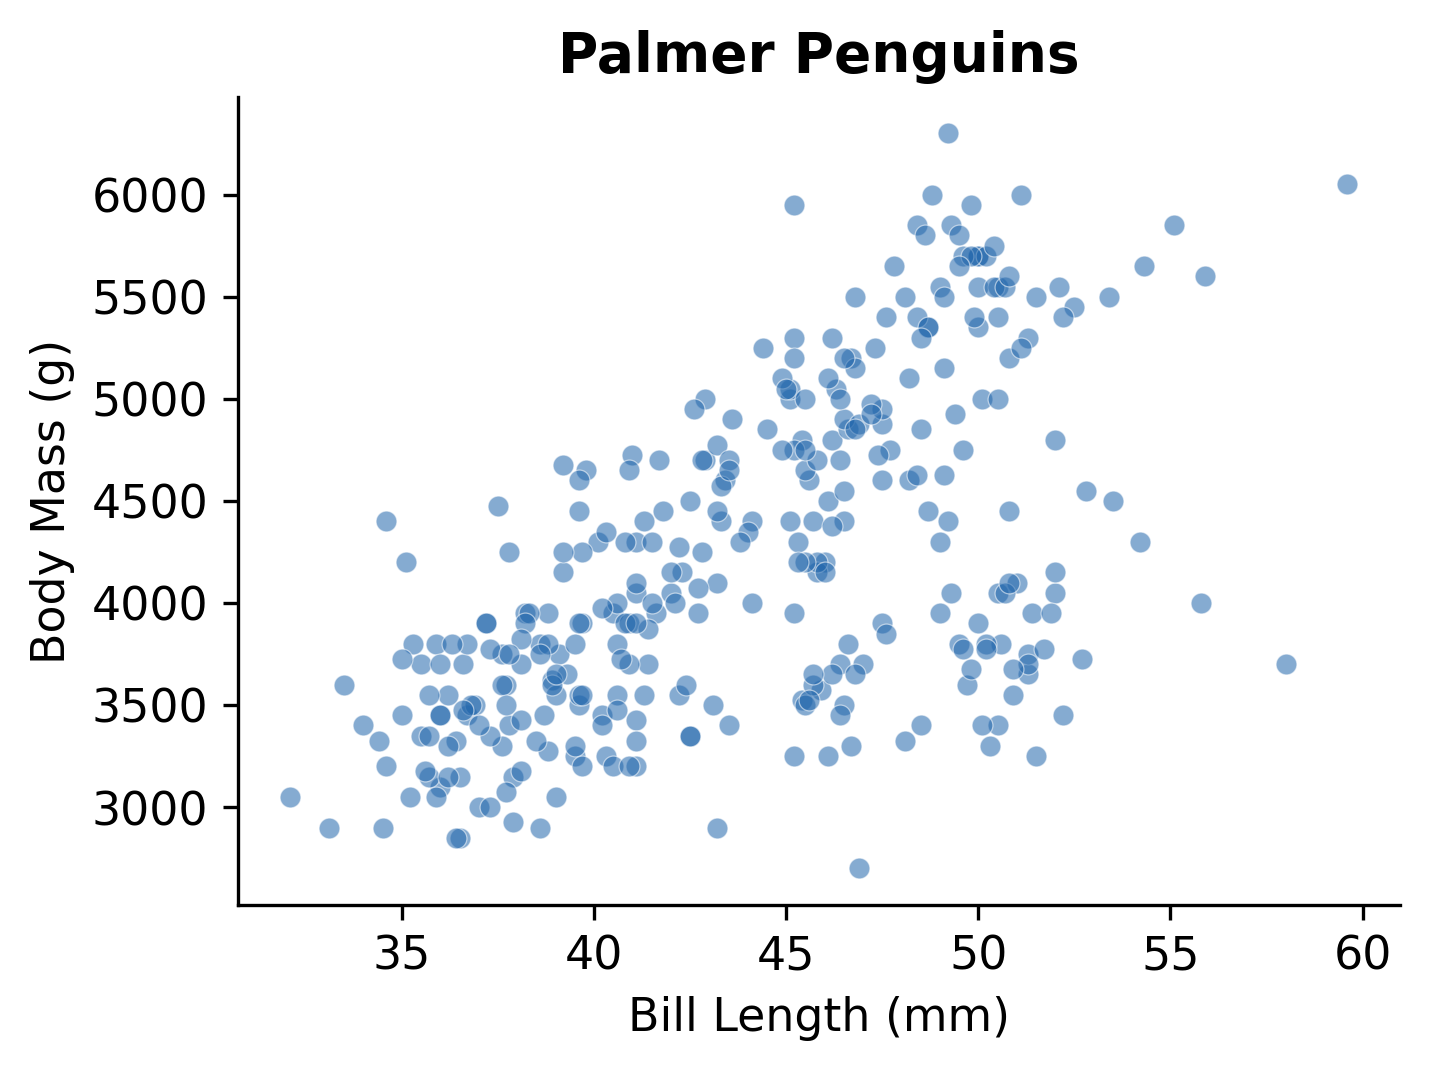
\includegraphics[width=\textwidth]{m1_3_scatter_basic.png}
\begin{alertblock}{Pro-Tip}
    \scriptsize Four variables: $x$, $y$, color, size, shape. Beyond 4 channels, legibility degrades fast.
\end{alertblock}
\end{column}
\end{columns}
\end{frame}

% ── 69 ──
\begin{frame}[fragile]{Adding Size and Shape --- \Python}\smark{69/300}
\begin{columns}[T]
\begin{column}{0.55\textwidth}
\begin{lstlisting}[style=Pystyle]
(ggplot(penguins,
   aes("bill_length_mm",
       "body_mass_g",
       color="species",
       size="bill_depth_mm",
       shape="island"))
 + geom_point(alpha=0.7)
 + scale_size_continuous(
     range=(1, 5))
 + theme_minimal())
\end{lstlisting}
\scriptref{scripts/m1\_3\_scatter\_multi\_aes.py}
\end{column}
\begin{column}{0.42\textwidth}
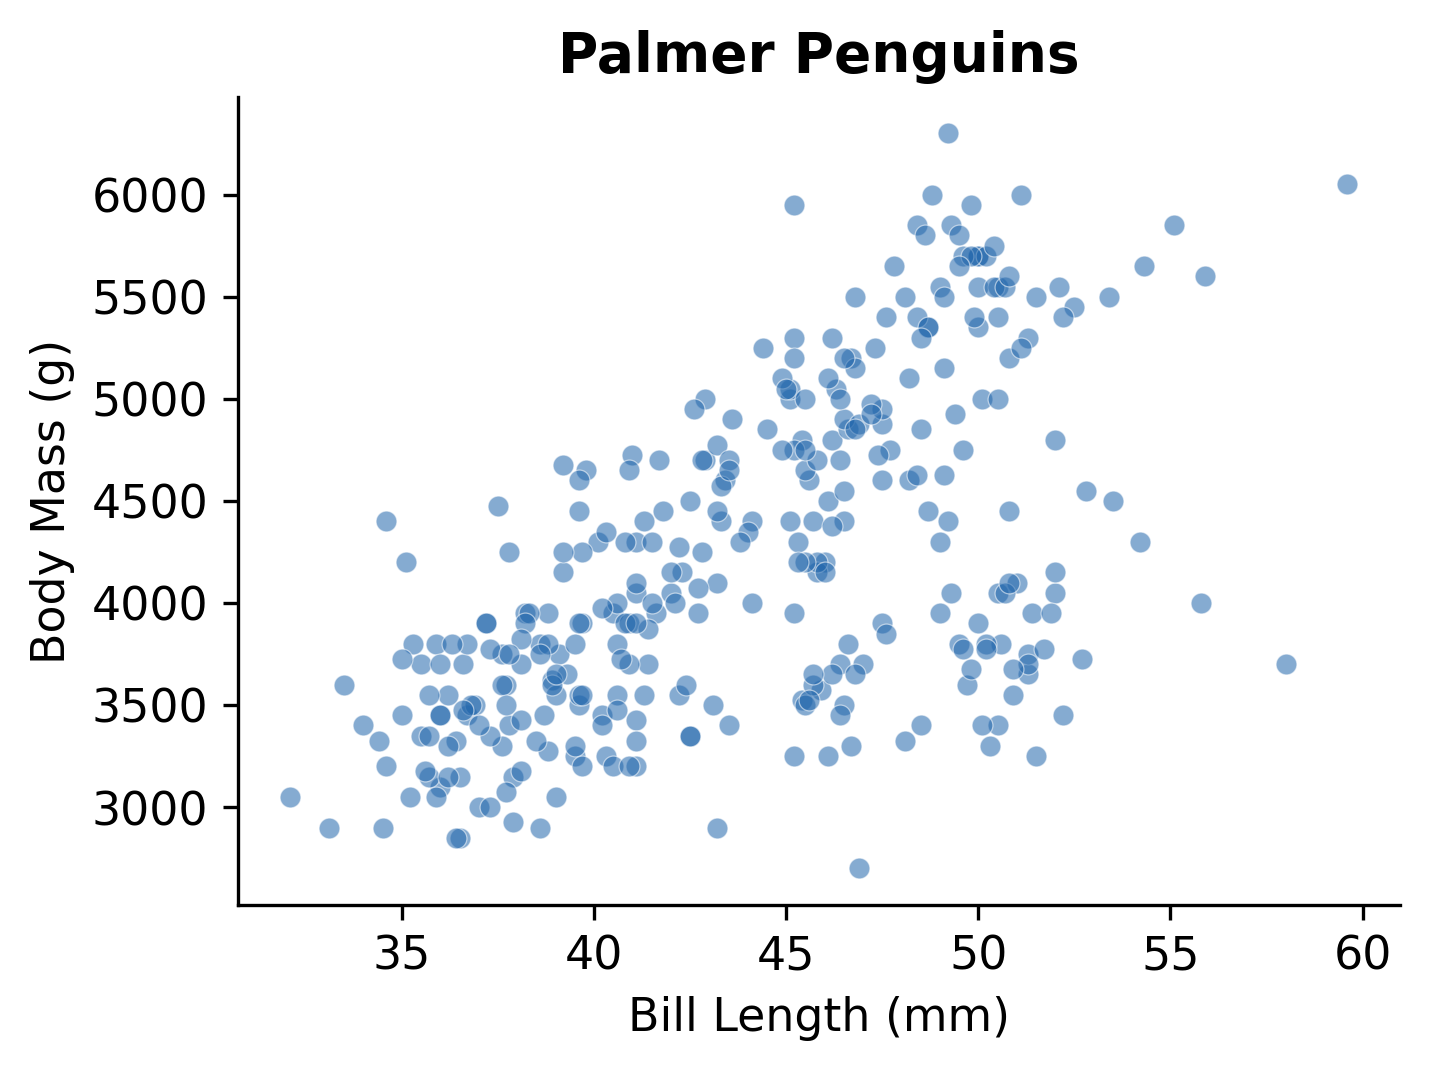
\includegraphics[width=\textwidth]{m1_3_scatter_basic.png}
\begin{exampleblock}{Data Insight}
    \scriptsize Shape has only 6 distinguishable levels. For more groups, use faceting instead.
\end{exampleblock}
\end{column}
\end{columns}
\end{frame}

% ── 70 ──
\begin{frame}{Overplotting: The Hidden Data Problem}
\smark{70/300}
\begin{columns}[T]
\begin{column}{0.50\textwidth}
\begin{itemize}
    \item Points stack on top of each other
    \item Density is invisible: 100 points look like 10
    \item Correlations and clusters are \textbf{masked}
    \item Worse with large $n$ or rounded/discrete data
\end{itemize}
\end{column}
\begin{column}{0.47\textwidth}
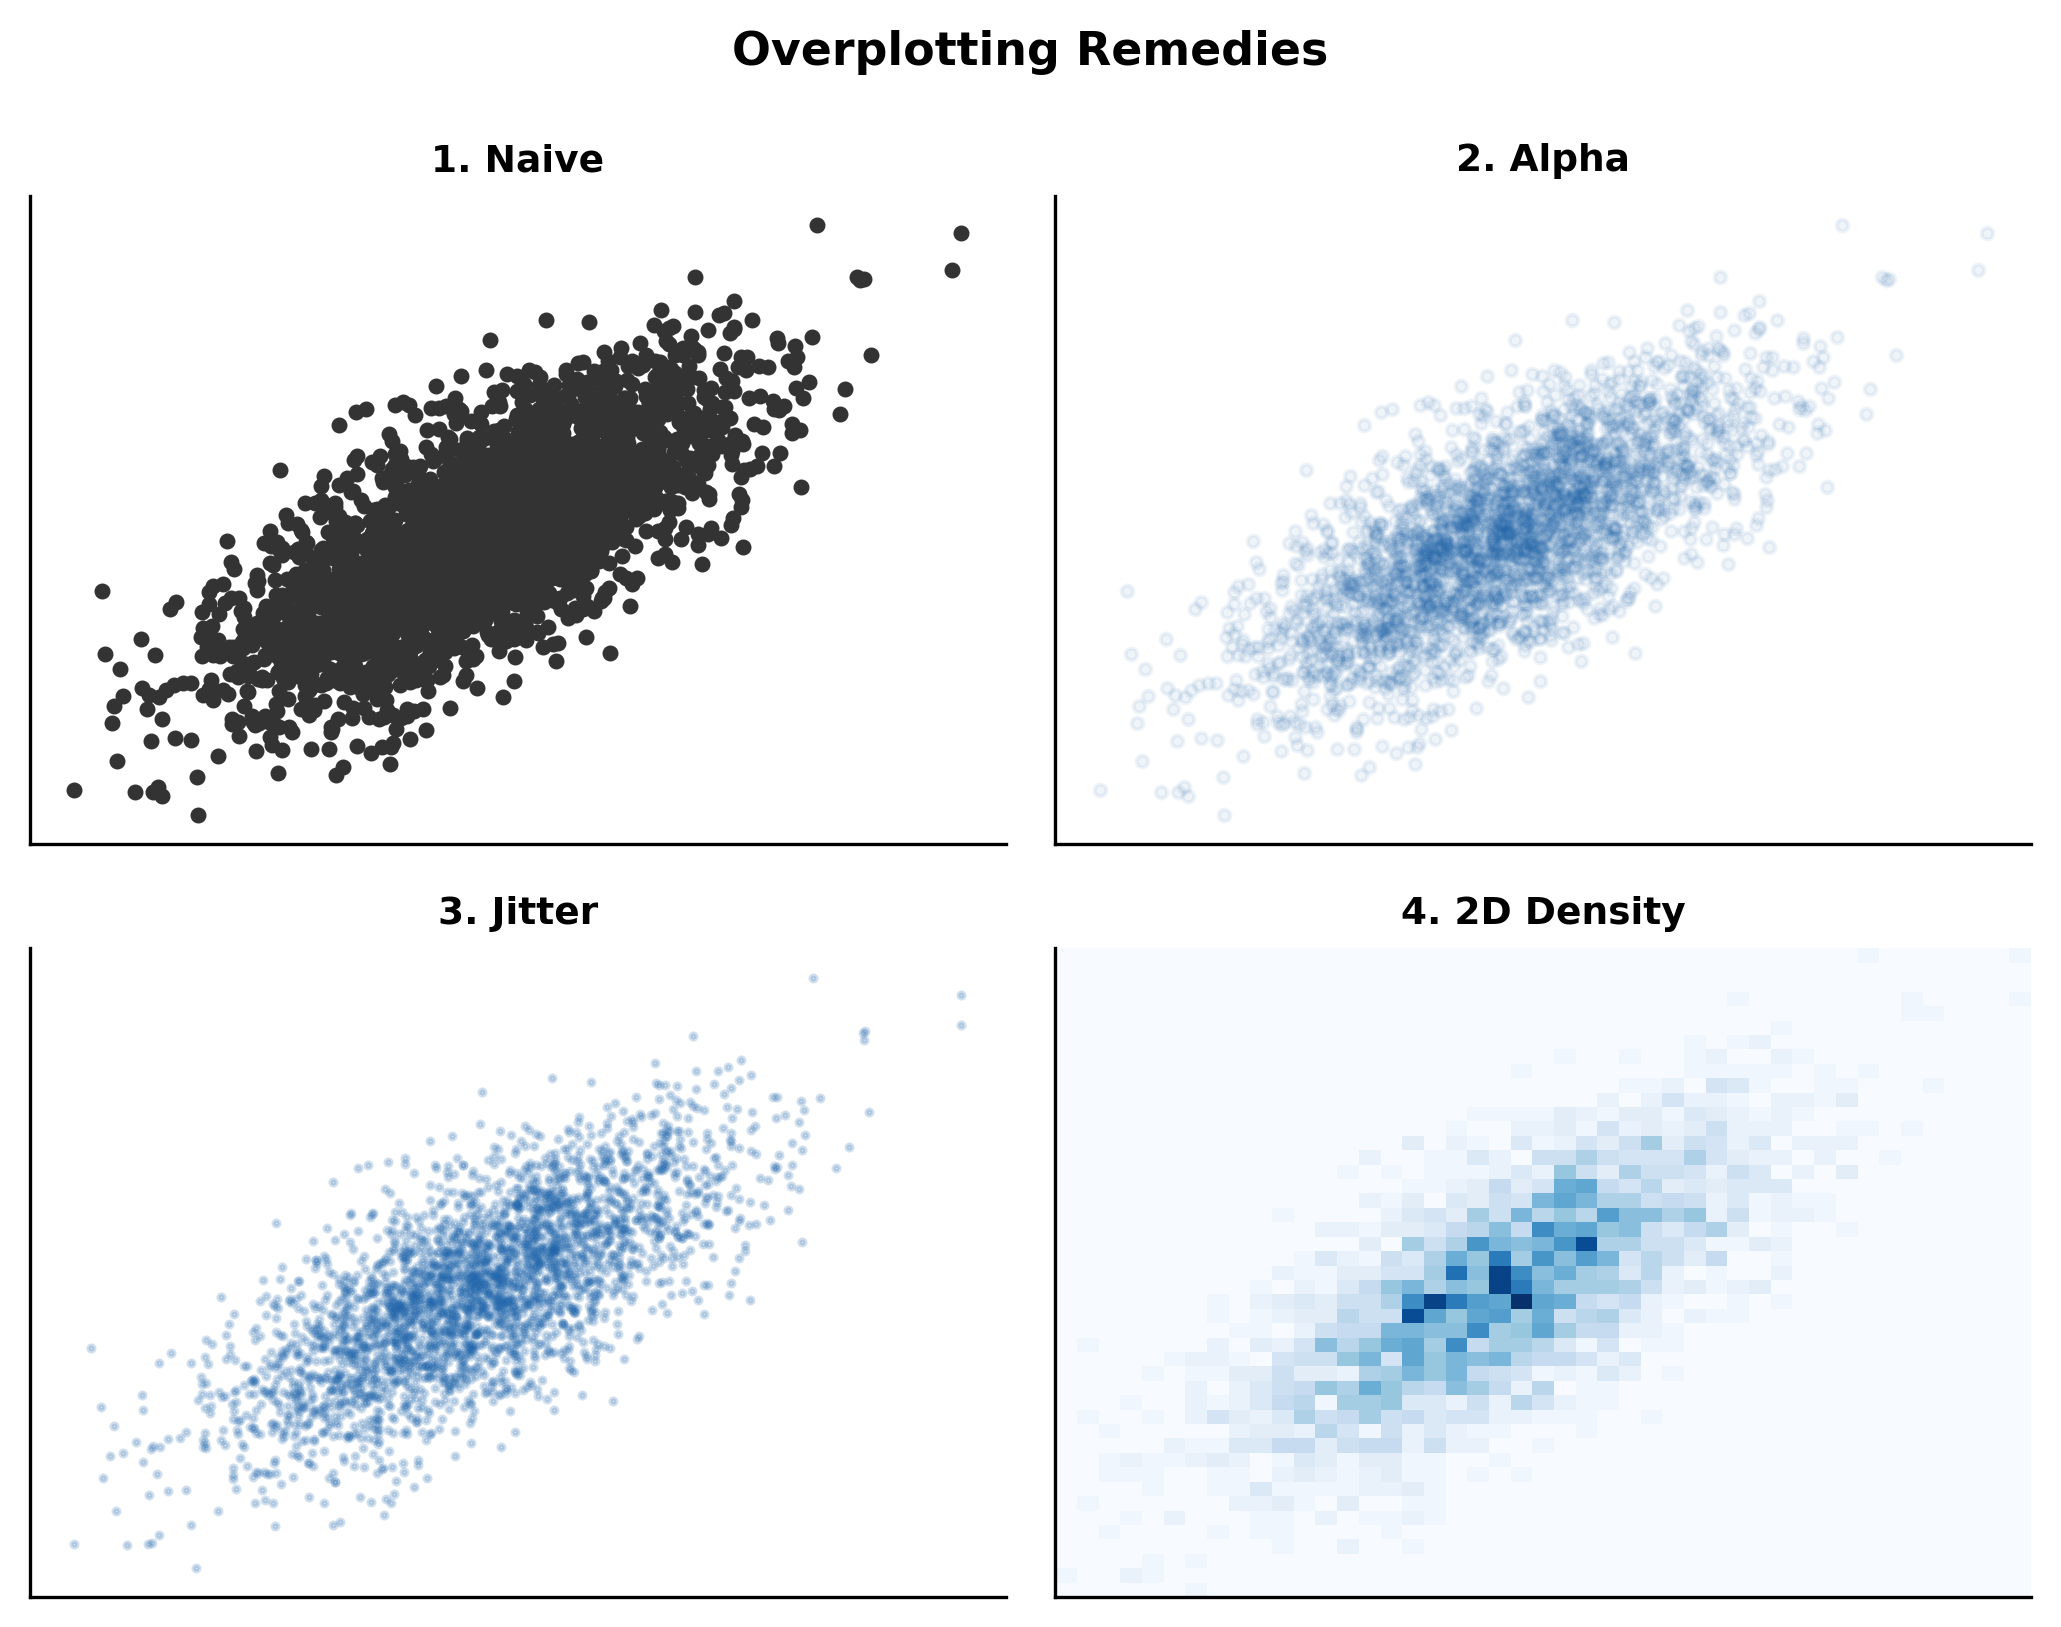
\includegraphics[width=\textwidth]{m1_3_overplotting.png}\\
{\scriptsize\color{codegray} 2000 points, all black, $\alpha=1$}
\vspace{0.2cm}
\begin{alertblock}{Pro-Tip}
    \scriptsize If your scatter looks like a solid blob, you have overplotting. Four fixes on the next slides.
\end{alertblock}
\end{column}
\end{columns}
\end{frame}

% ── 71 ──
\begin{frame}{Four Overplotting Remedies}
\smark{71/300}
\centering\small
\begin{tabular}{@{}clll@{}}
    \toprule
    \# & \textbf{Remedy} & \textbf{Best When} & \textbf{Grammar} \\
    \midrule
    1 & Alpha transparency & Moderate overlap    & \texttt{alpha = 0.1} \\
    2 & Jitter             & Discrete/rounded $x$/$y$ & \texttt{geom\_jitter()} \\
    3 & Small point size   & Very large $n$      & \texttt{size = 0.3} \\
    4 & 2D density         & Massive $n$ ($>$10K) & \texttt{geom\_density\_2d()} \\
    \bottomrule
\end{tabular}

\vspace{0.4cm}
\begin{exampleblock}{Data Insight}
    \scriptsize These are cumulative: combine alpha + small size for $n = 50$K, or switch to a 2D density/hex bin for $n > 100$K.
\end{exampleblock}
\end{frame}

% ── 72 ──
\begin{frame}[fragile]{Overplotting Fixes --- \Rlang}\smark{72/300}
\begin{columns}[T]
\begin{column}{0.55\textwidth}
\begin{lstlisting}[style=Rstyle]
# 1. Alpha
ggplot(df, aes(x, y)) +
  geom_point(alpha = 0.1)

# 2. Jitter
ggplot(df, aes(x, y)) +
  geom_jitter(width=0.2, height=0.2,
              alpha=0.3, size=0.5)

# 3. 2D density contour
ggplot(df, aes(x, y)) +
  geom_density_2d_filled() +
  theme(legend.position="none")
\end{lstlisting}
\scriptref{scripts/m1\_3\_overplotting.R}
\end{column}
\begin{column}{0.42\textwidth}
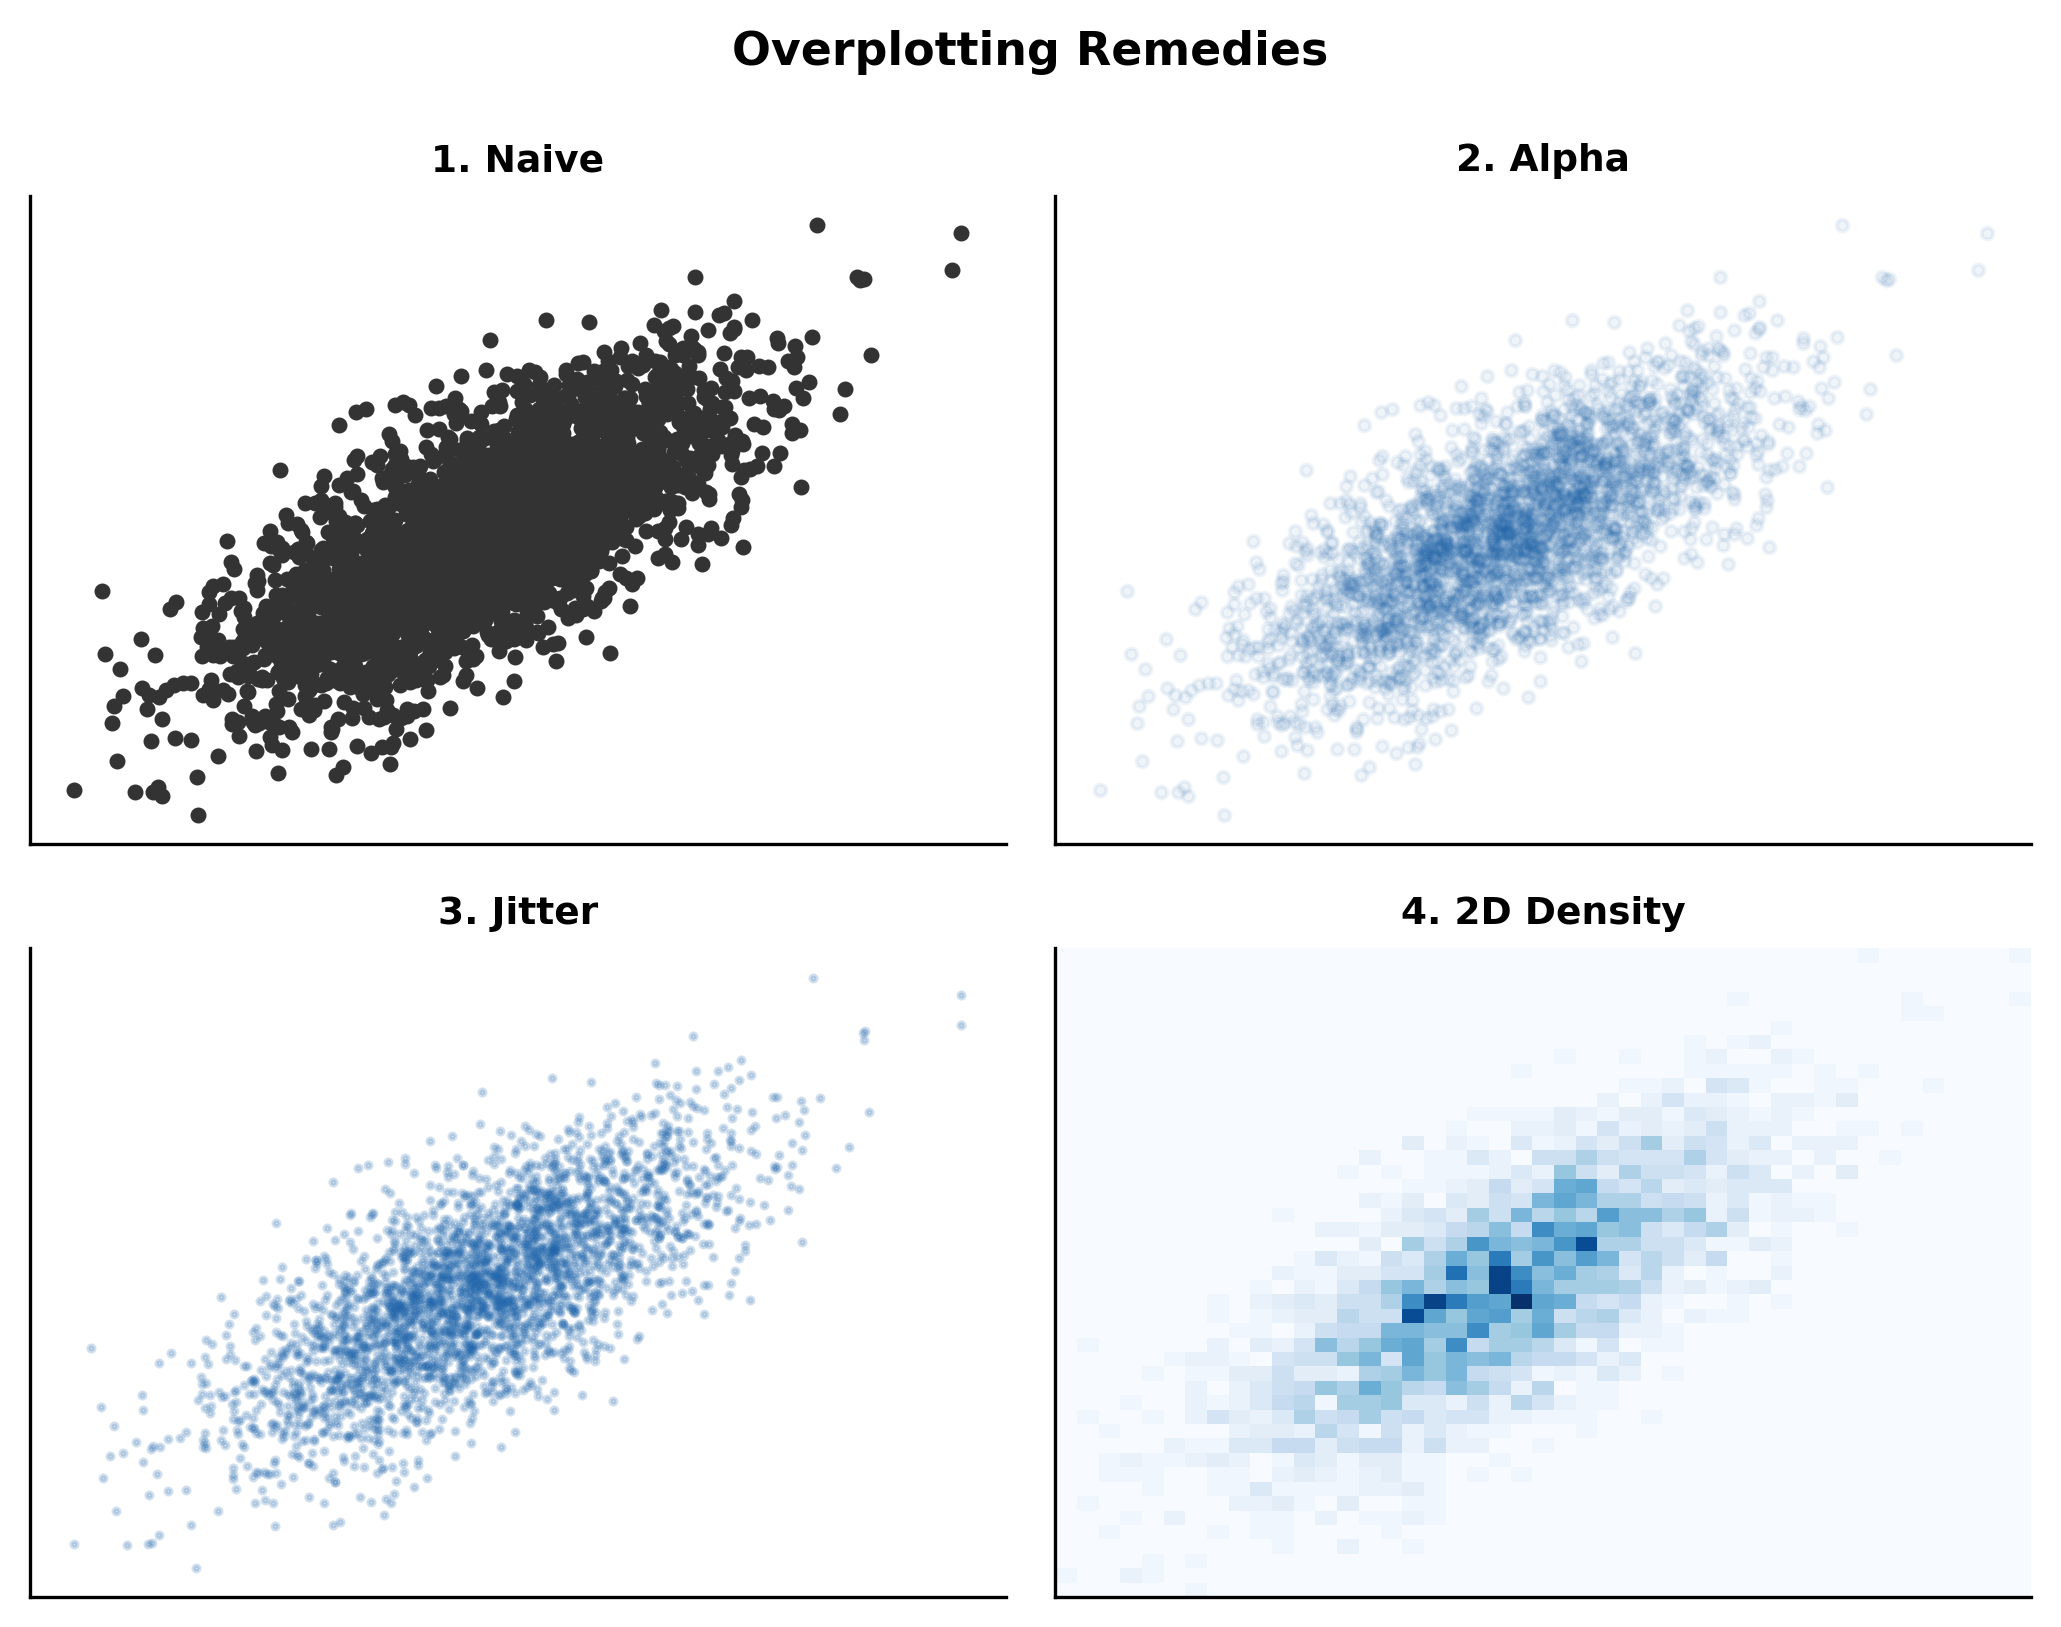
\includegraphics[width=\textwidth]{m1_3_overplotting.png}
\begin{exampleblock}{Data Insight}
    \scriptsize Alpha reveals the high-density core. Density contours show the exact bivariate distribution shape.
\end{exampleblock}
\end{column}
\end{columns}
\end{frame}

% ── 73 ──
\begin{frame}[fragile]{Overplotting Fixes --- \Python}\smark{73/300}
\begin{columns}[T]
\begin{column}{0.55\textwidth}
\begin{lstlisting}[style=Pystyle]
# 1. Alpha
ax.scatter(x, y, alpha=0.1, s=10)

# 2. Jitter (add noise manually)
jx = x + np.random.uniform(-0.2,
                             0.2, len(x))
ax.scatter(jx, jy, alpha=0.3, s=3)

# 3. 2D histogram (density)
ax.hist2d(x, y, bins=40,
          cmap="Blues")
\end{lstlisting}
\scriptref{scripts/m1\_3\_overplotting.py}
\end{column}
\begin{column}{0.42\textwidth}
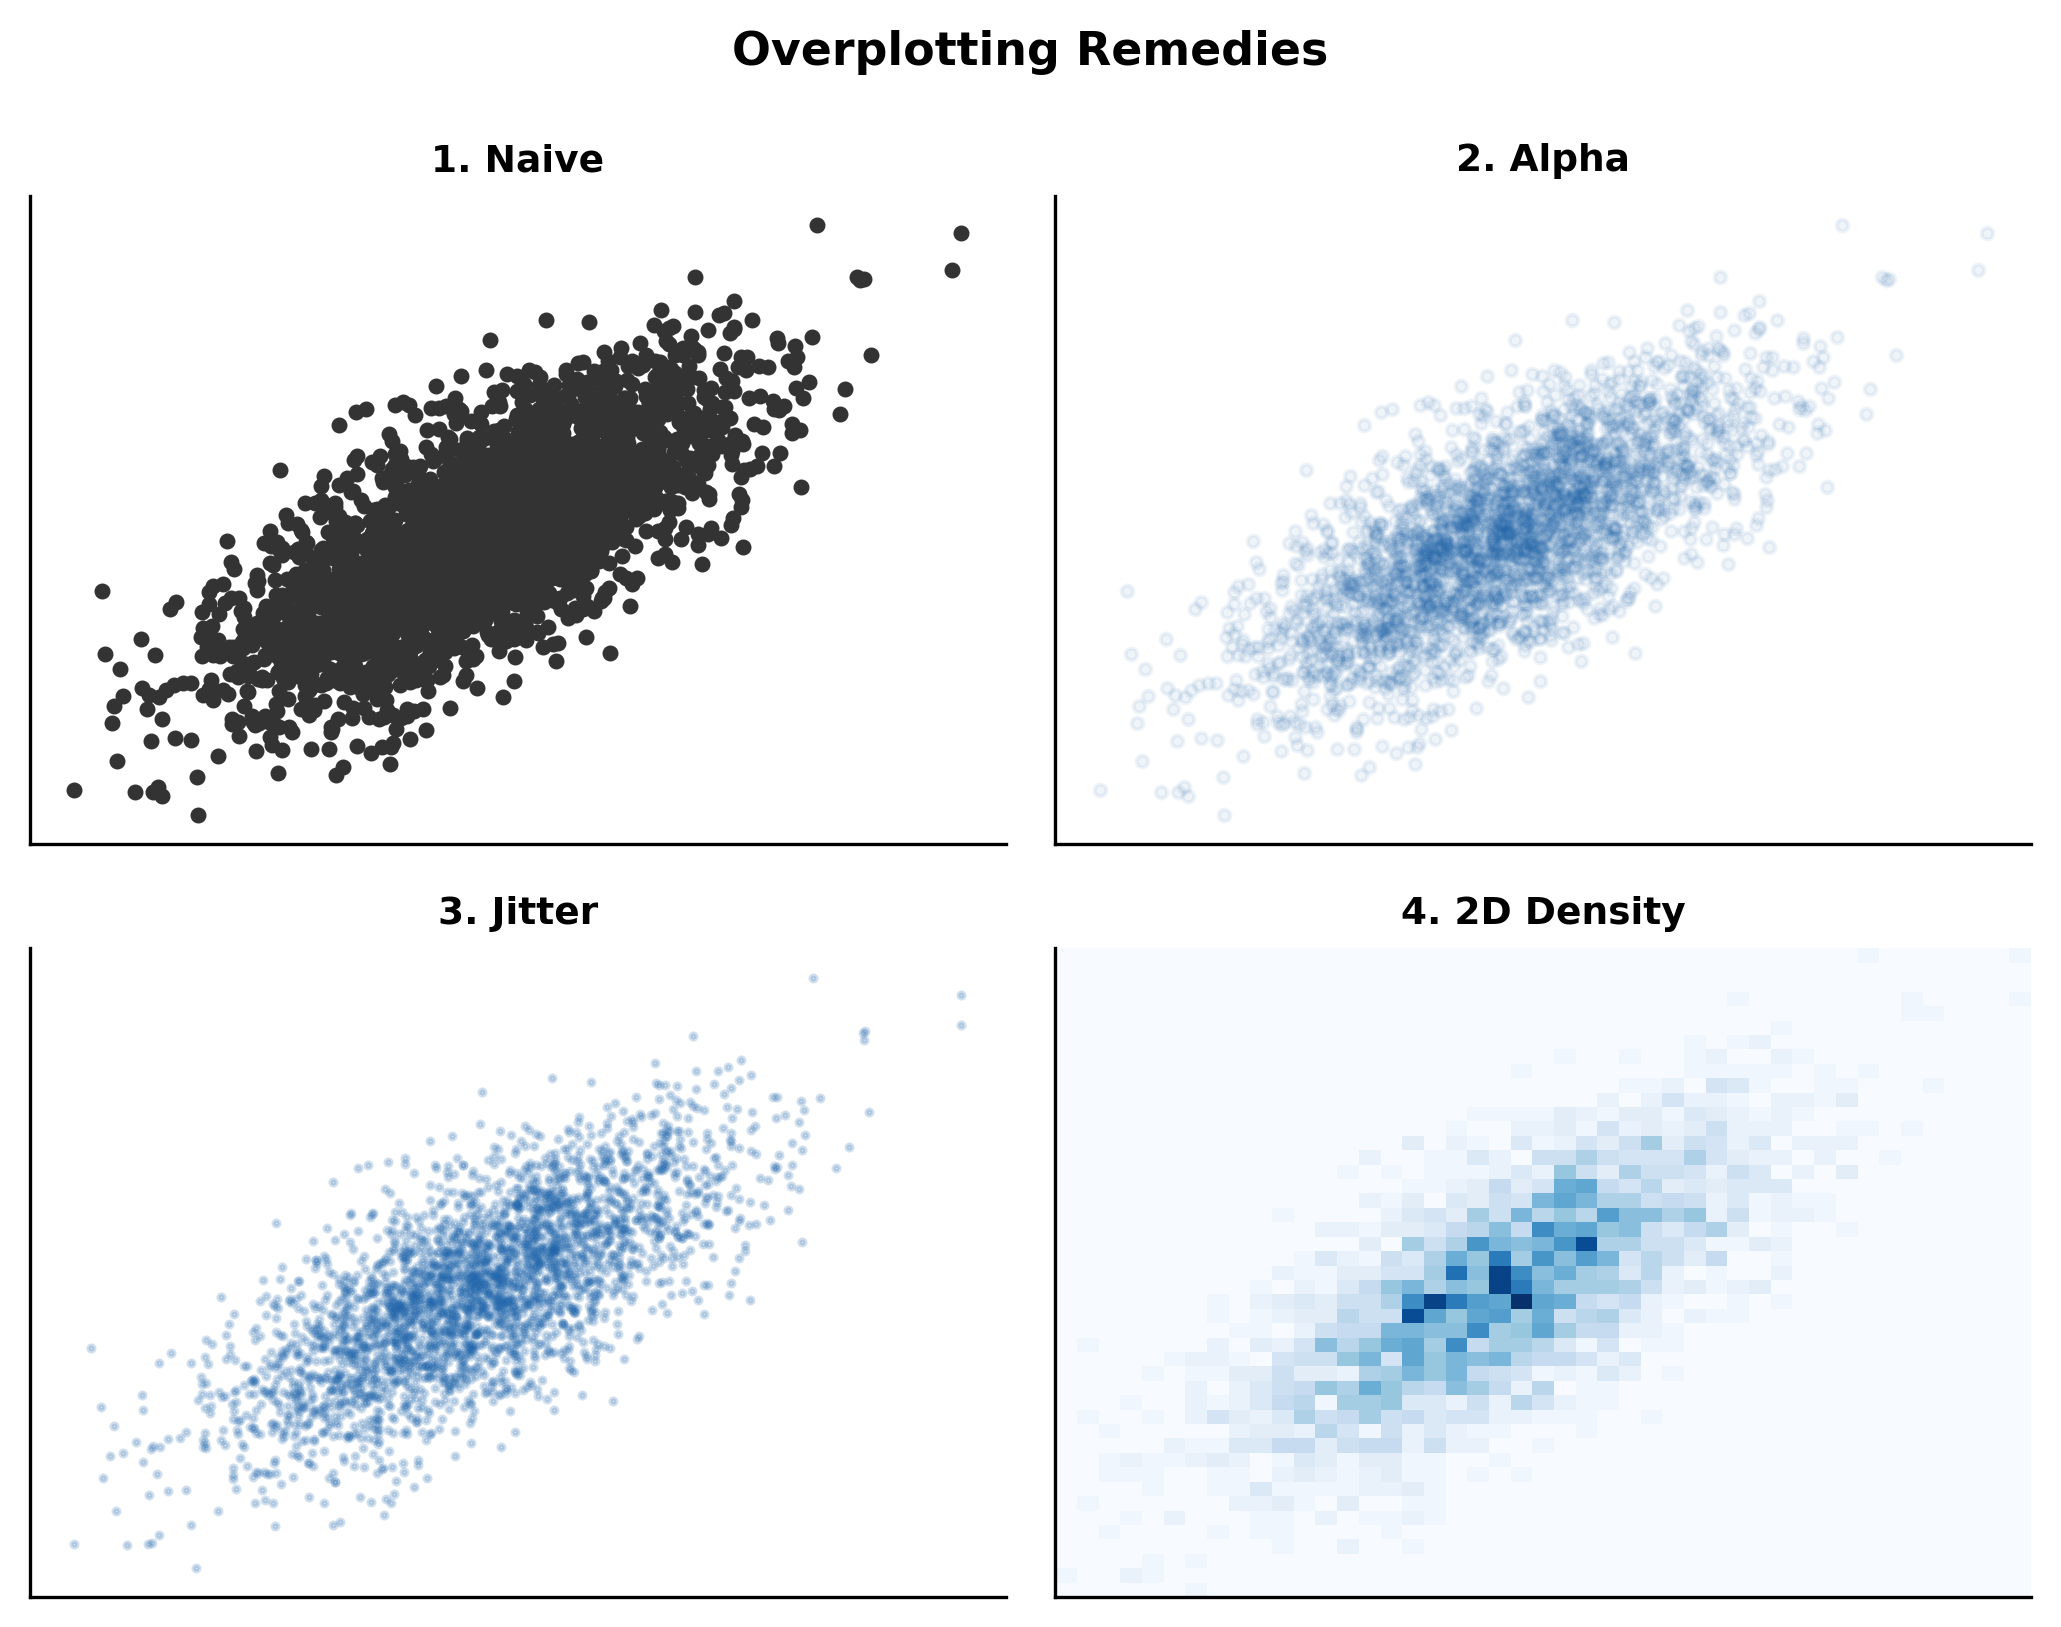
\includegraphics[width=\textwidth]{m1_3_overplotting.png}
\begin{alertblock}{Pro-Tip}
    \scriptsize \texttt{matplotlib} has no \texttt{geom\_jitter}. Add uniform noise manually. \texttt{plotnine} does have \texttt{geom\_jitter()}.
\end{alertblock}
\end{column}
\end{columns}
\end{frame}

% ── 74 ──
\begin{frame}{The Bar Chart: When and Why}
\smark{74/300}
\begin{columns}[T]
\begin{column}{0.50\textwidth}
\begin{itemize}
    \item Compares \textbf{magnitudes} across categories
    \item Uses \textbf{length} encoding (rank 3)
    \item Baseline \textbf{must start at zero}
    \item Categorical $x$, continuous $y$
\end{itemize}
\end{column}
\begin{column}{0.47\textwidth}
\begin{alertblock}{Pro-Tip}
    \scriptsize Truncating the y-axis on a bar chart is a \textbf{cardinal sin} --- it distorts length encoding. Dot plots are the alternative for non-zero baselines.
\end{alertblock}
\vspace{0.2cm}
\begin{exampleblock}{Data Insight}
    \scriptsize Bar = position + length. Pie = angle + area. That is why bars are almost always superior.
\end{exampleblock}
\end{column}
\end{columns}
\end{frame}

% ── 75 ──
\begin{frame}{Sorting Bars: Alphabet vs.\ Value}
\smark{75/300}
\begin{columns}[T]
\begin{column}{0.48\textwidth}
\centering
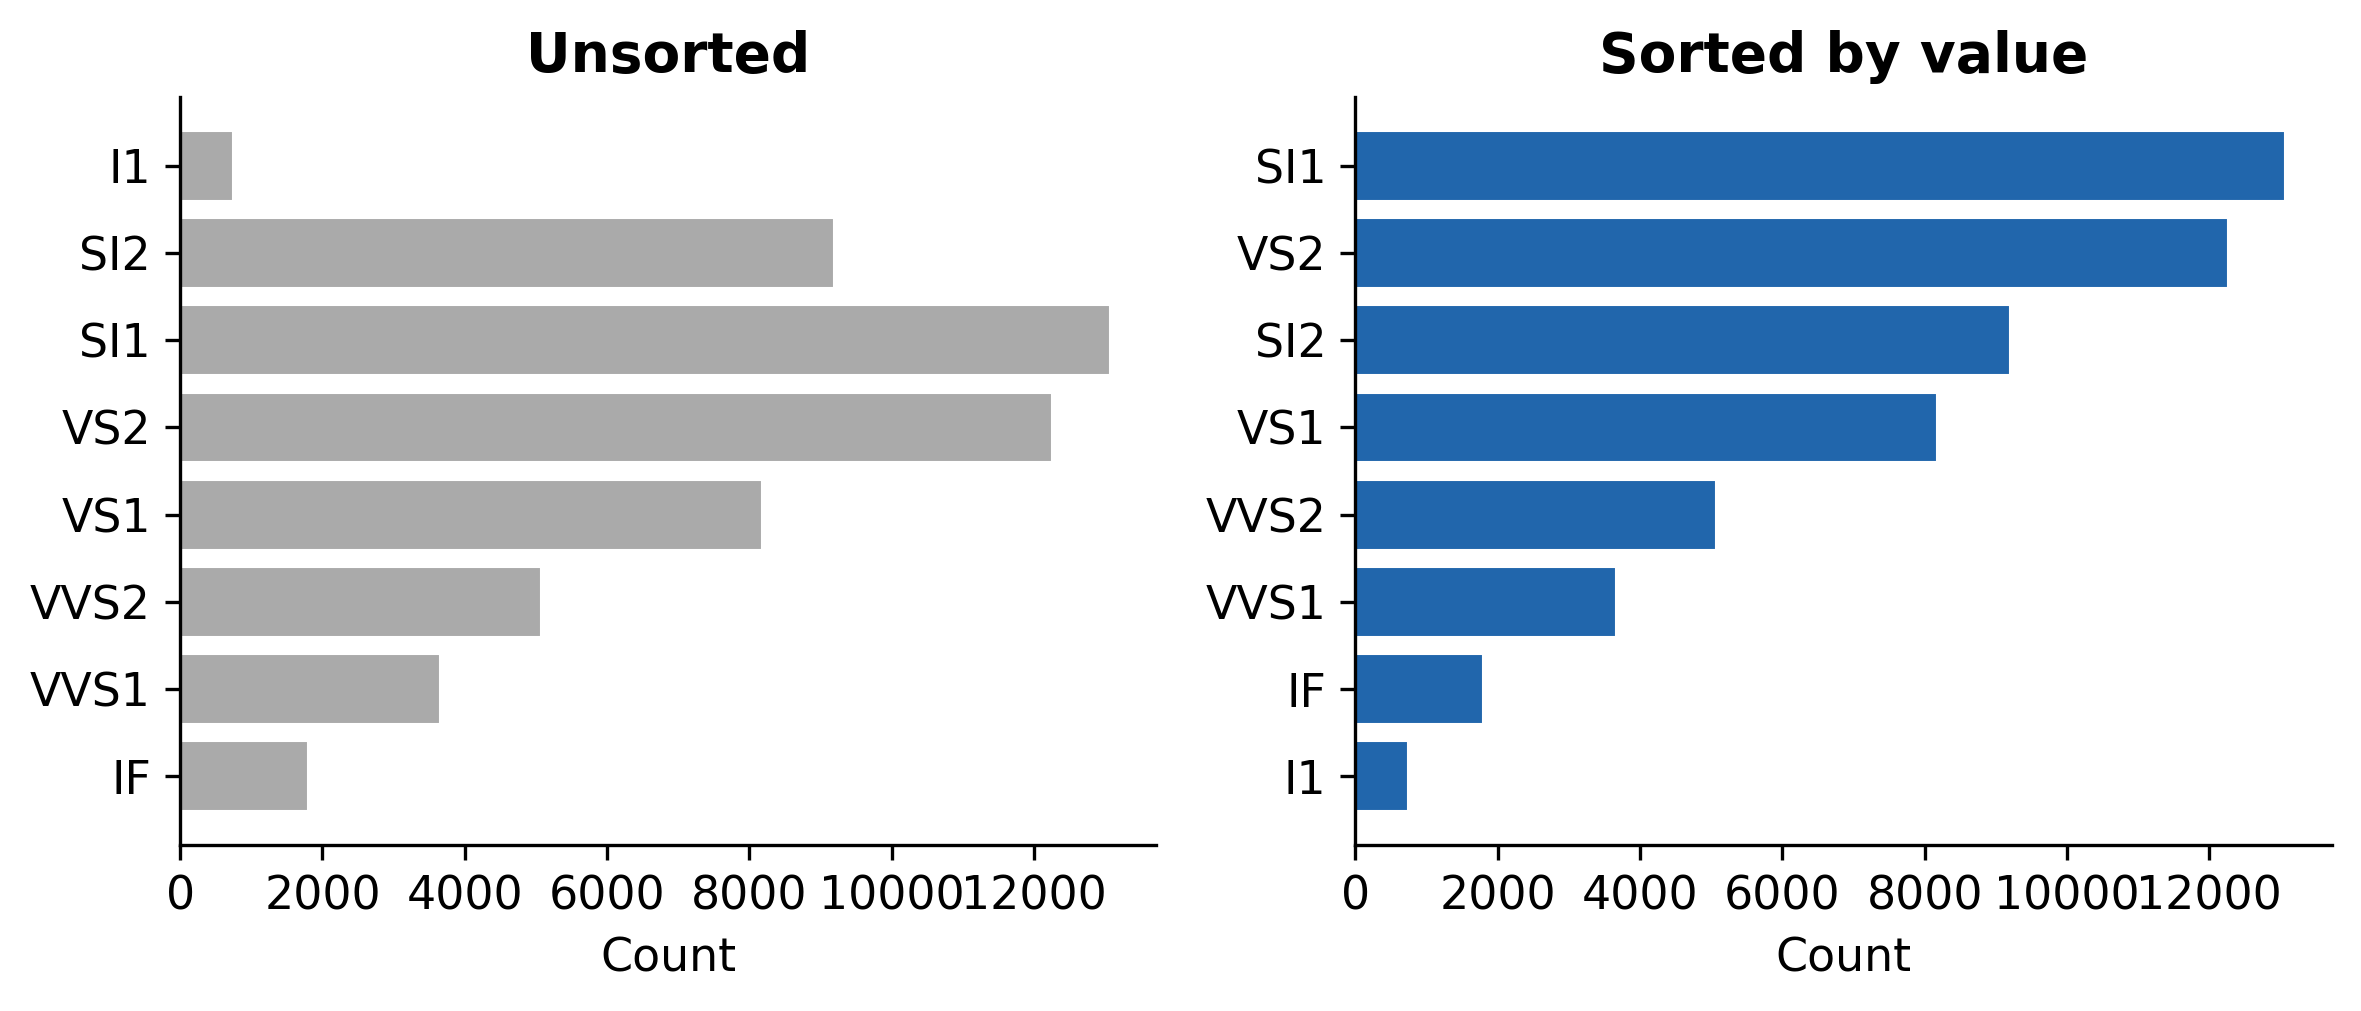
\includegraphics[width=\textwidth]{m1_3_bar_sorted.png}\\
{\scriptsize\color{codegray} Unsorted (alphabetical)}
\end{column}
\begin{column}{0.48\textwidth}
\centering
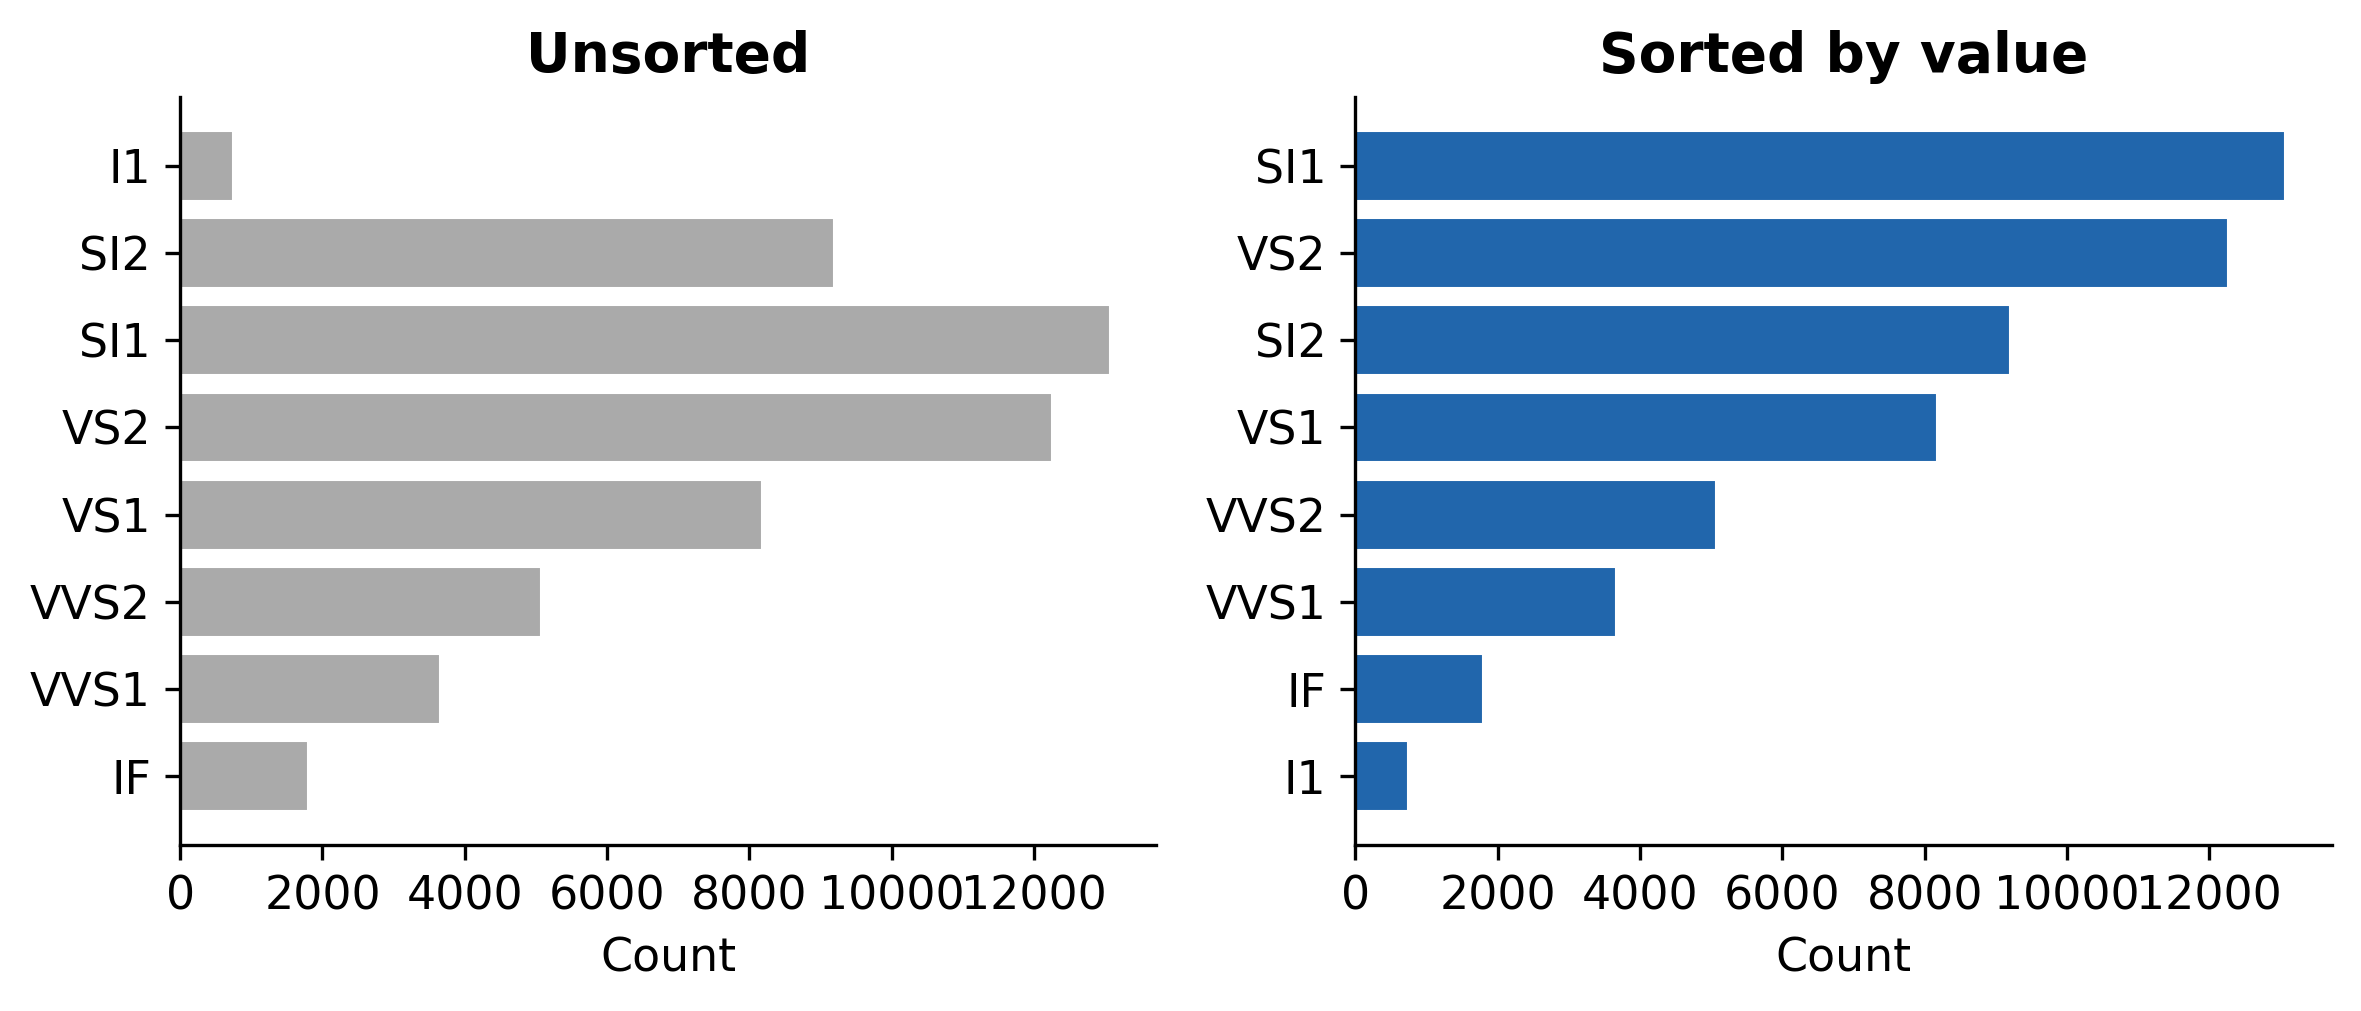
\includegraphics[width=\textwidth]{m1_3_bar_sorted.png}\\
{\scriptsize\color{codegray} Sorted by value}
\end{column}
\end{columns}
\vspace{0.3cm}
\begin{exampleblock}{Data Insight}
    \scriptsize Sort by value unless categories have intrinsic order (e.g., ``Poor'' $\to$ ``Excellent''). Alphabetical forces \textbf{serial} comparison.
\end{exampleblock}
\end{frame}

% ── 76 ──
\begin{frame}[fragile]{Sorted Bar Chart --- \Rlang}\smark{76/300}
\begin{columns}[T]
\begin{column}{0.55\textwidth}
\begin{lstlisting}[style=Rstyle]
library(forcats)
df <- diamonds |> count(clarity)

# fct_reorder sorts by n
ggplot(df,
  aes(fct_reorder(clarity, n),
      n)) +
  geom_col(fill = "#2166AC") +
  coord_flip() +
  labs(x="Clarity", y="Count") +
  theme_minimal()
\end{lstlisting}
\scriptref{scripts/m1\_3\_bar\_variations.R}
\end{column}
\begin{column}{0.42\textwidth}
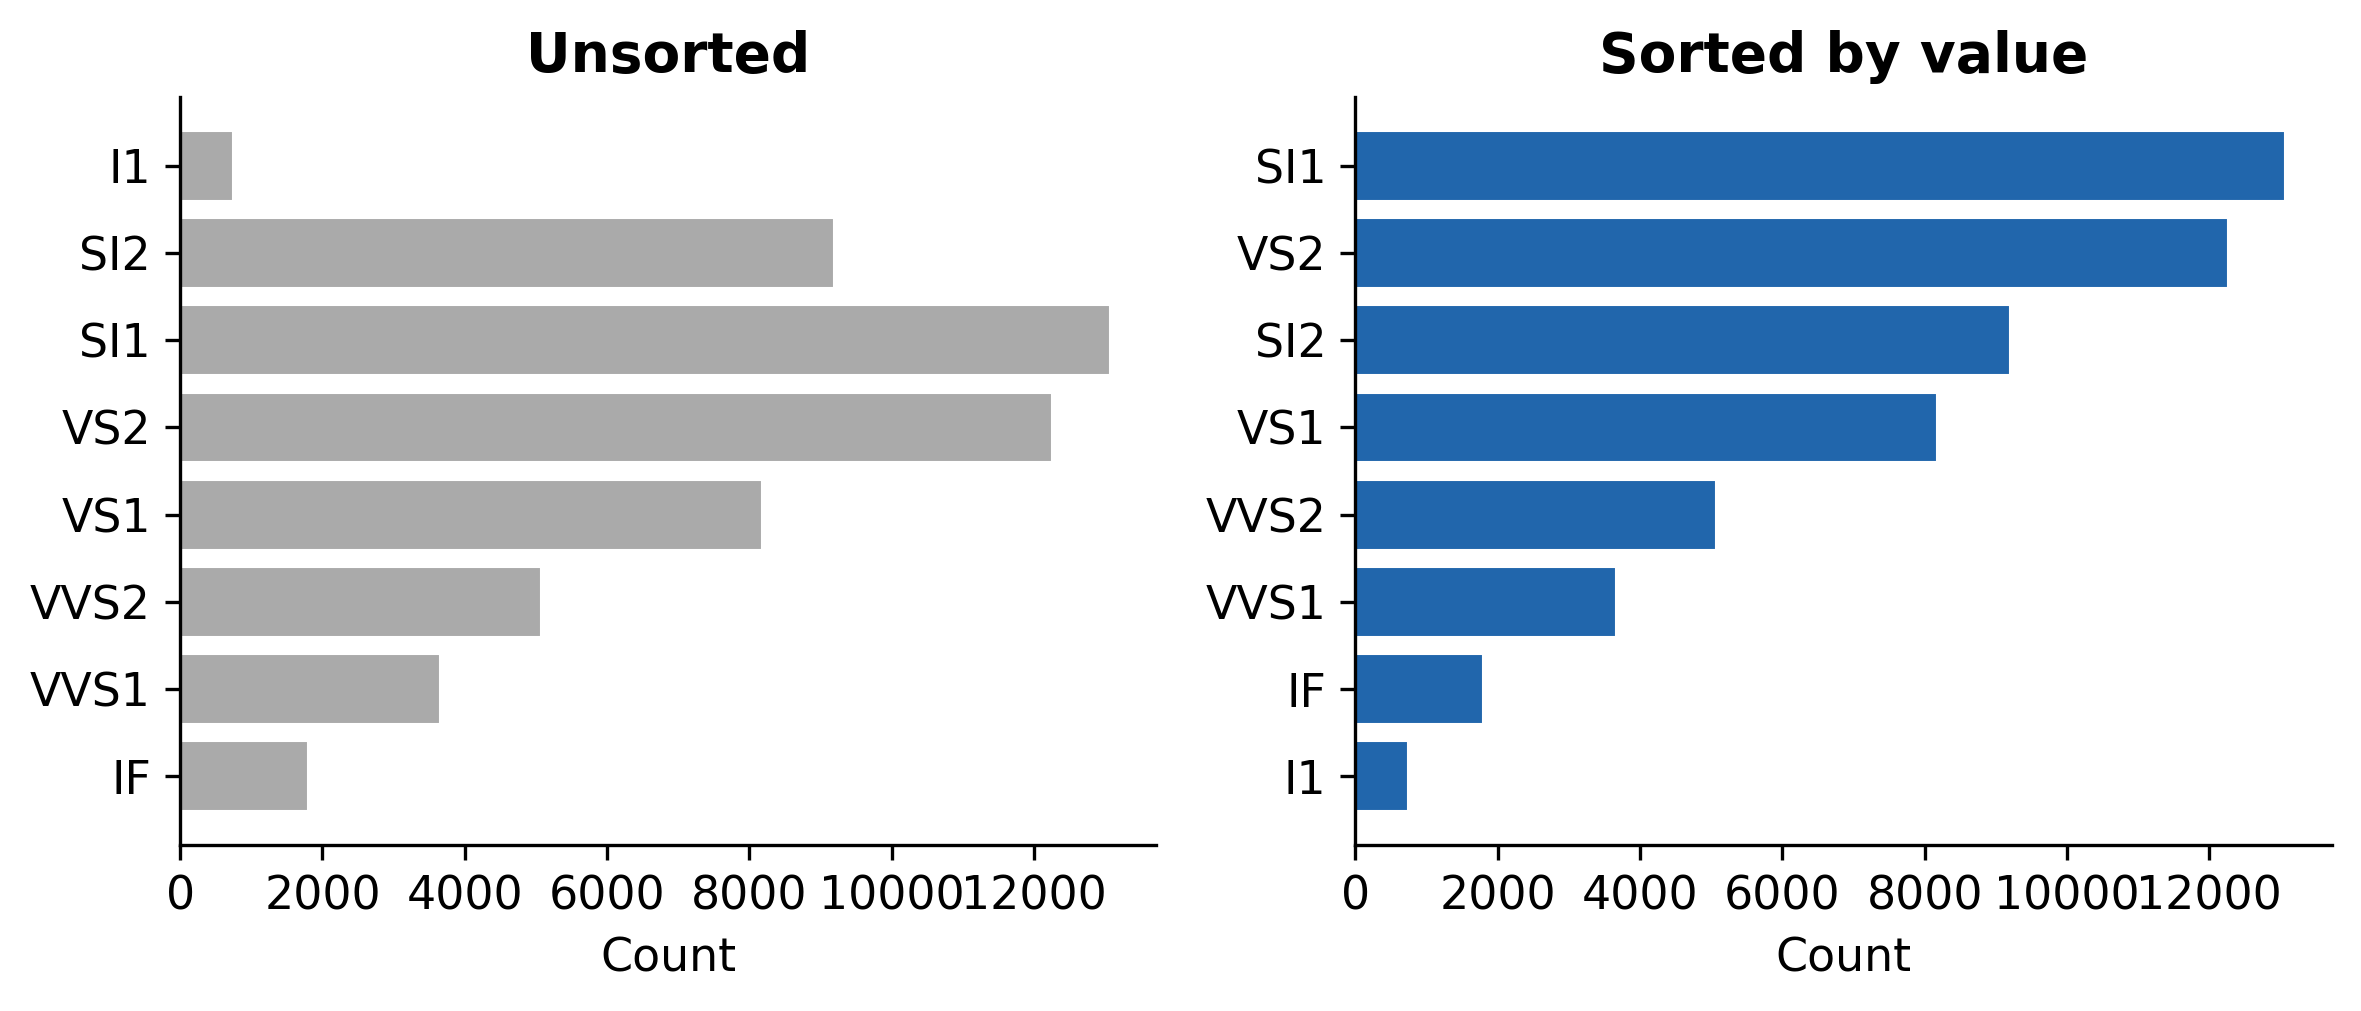
\includegraphics[width=\textwidth]{m1_3_bar_sorted.png}
\begin{alertblock}{Pro-Tip}
    \scriptsize \texttt{forcats::fct\_reorder()} reorders a factor by a numeric variable. Essential for clean bars.
\end{alertblock}
\end{column}
\end{columns}
\end{frame}

% ── 77 ──
\begin{frame}[fragile]{Sorted Bar Chart --- \Python}\smark{77/300}
\begin{columns}[T]
\begin{column}{0.55\textwidth}
\begin{lstlisting}[style=Pystyle]
diamonds = sns.load_dataset("diamonds")
df = (diamonds["clarity"]
      .value_counts()
      .reset_index())
df.columns = ["clarity", "n"]
dfs = df.sort_values("n")

plt.barh(dfs["clarity"], dfs["n"],
         color="#B2182B")
plt.xlabel("Count")
plt.ylabel("Clarity")
\end{lstlisting}
\scriptref{scripts/m1\_3\_bar\_variations.py}
\end{column}
\begin{column}{0.42\textwidth}
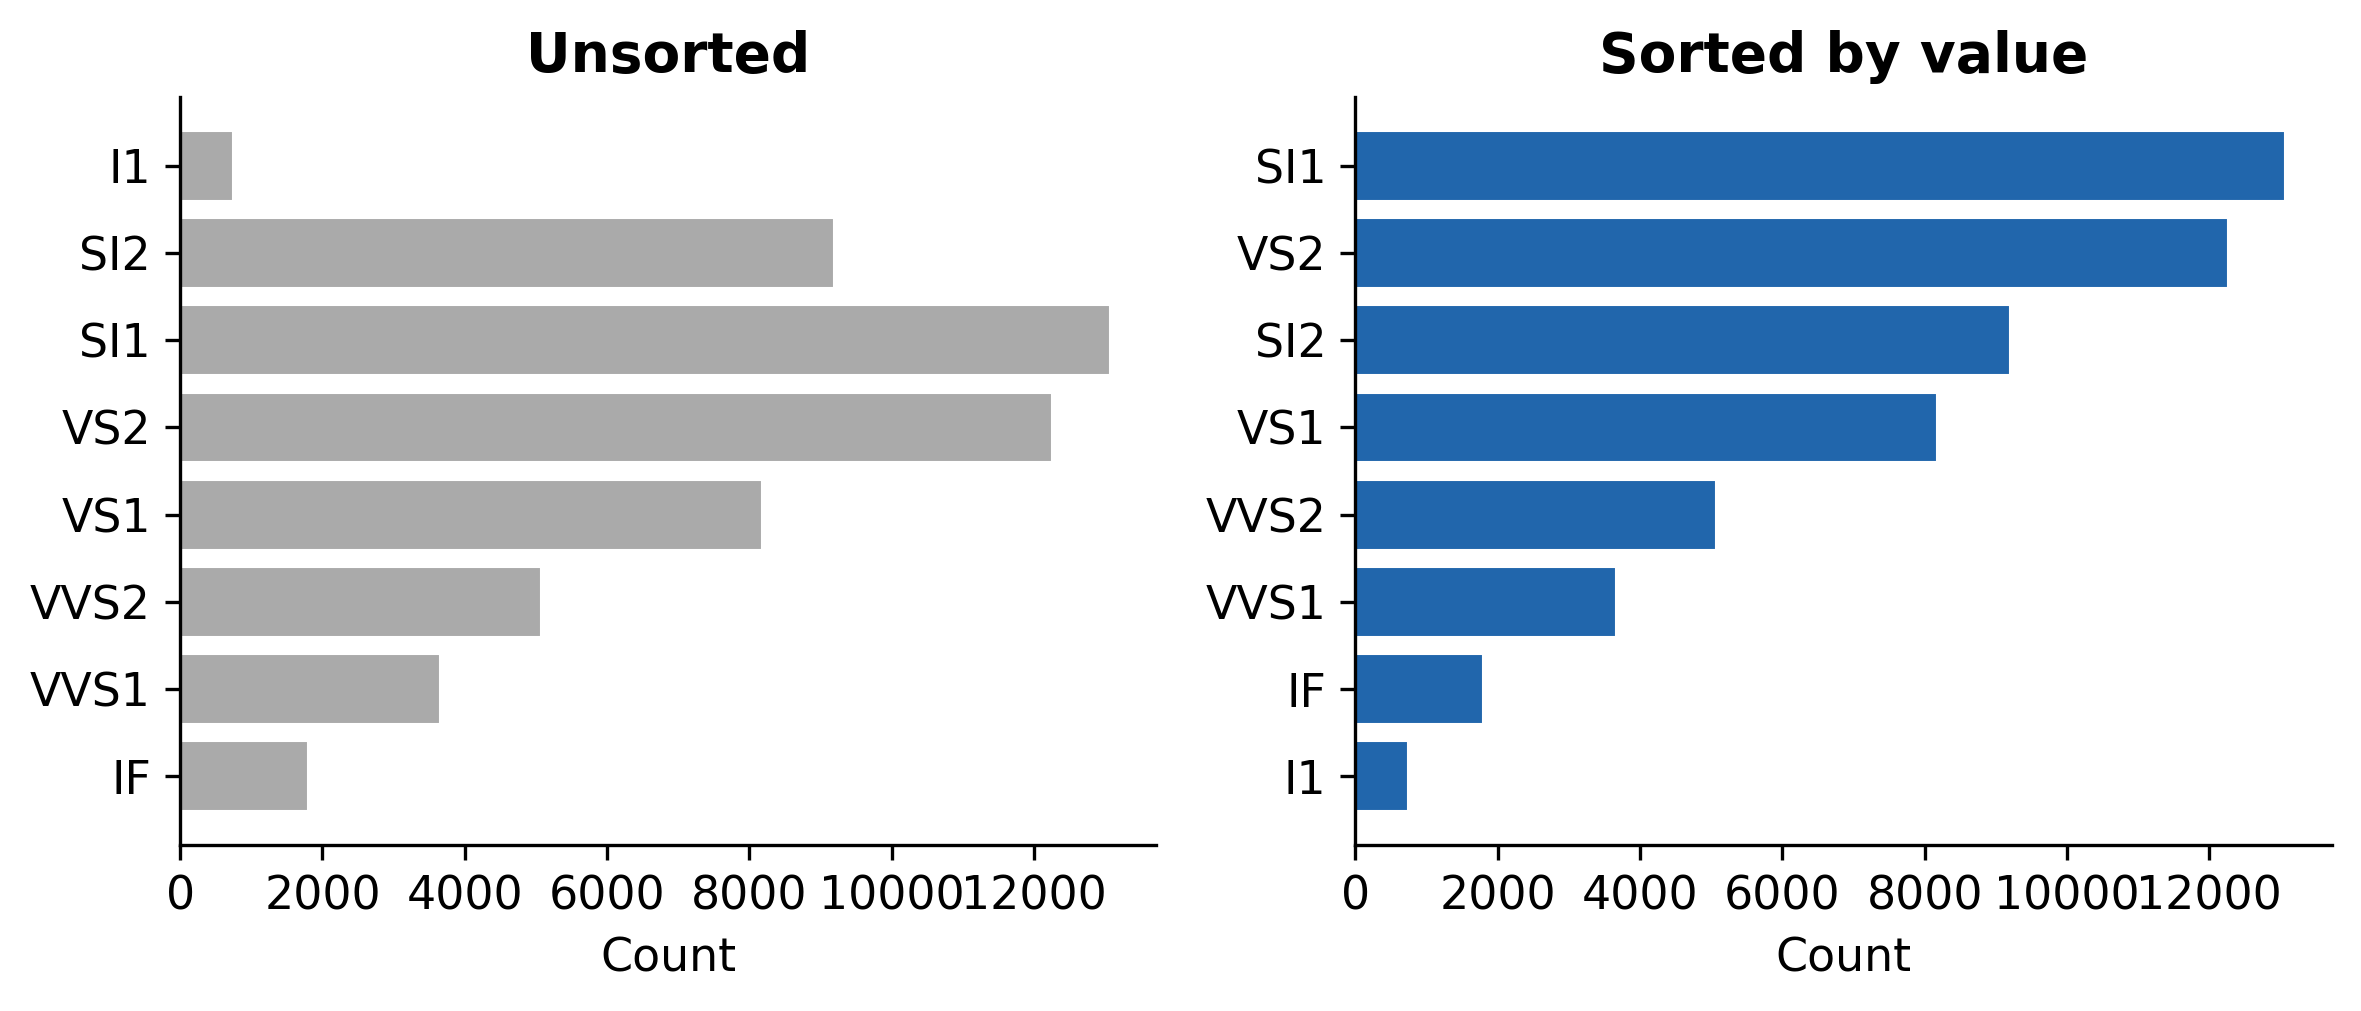
\includegraphics[width=\textwidth]{m1_3_bar_sorted.png}
\begin{alertblock}{Pro-Tip}
    \scriptsize \texttt{sort\_values()} before plotting. matplotlib plots bars in the order you provide.
\end{alertblock}
\end{column}
\end{columns}
\end{frame}

% ── 78 ──
\begin{frame}{Position Adjustments for Bars}
\smark{78/300}
\centering\small
\begin{tabular}{@{}lll@{}}
    \toprule
    \textbf{Position} & \textbf{Visual Effect} & \textbf{Best For} \\
    \midrule
    \texttt{stack}  & Segments stacked vertically  & Total + composition \\
    \texttt{dodge}  & Segments side by side         & Direct group comparison \\
    \texttt{fill}   & Stacked to 100\%              & Proportional comparison \\
    \texttt{jitter} & Random offset (scatter only)  & Overlapping discrete pts \\
    \bottomrule
\end{tabular}

\vspace{0.4cm}
\begin{exampleblock}{Data Insight}
    \scriptsize \texttt{stack} is default when \texttt{fill} aesthetic is mapped. Override with \texttt{position="dodge"} for direct segment comparison.
\end{exampleblock}
\end{frame}

% ── 79 ──
\begin{frame}[fragile]{Position: Stack vs.\ Dodge --- \Rlang}\smark{79/300}
\begin{columns}[T]
\begin{column}{0.48\textwidth}
\begin{lstlisting}[style=Rstyle]
# Stacked (default)
ggplot(diamonds,
  aes(cut, fill=clarity)) +
  geom_bar(position="stack")
\end{lstlisting}
\centering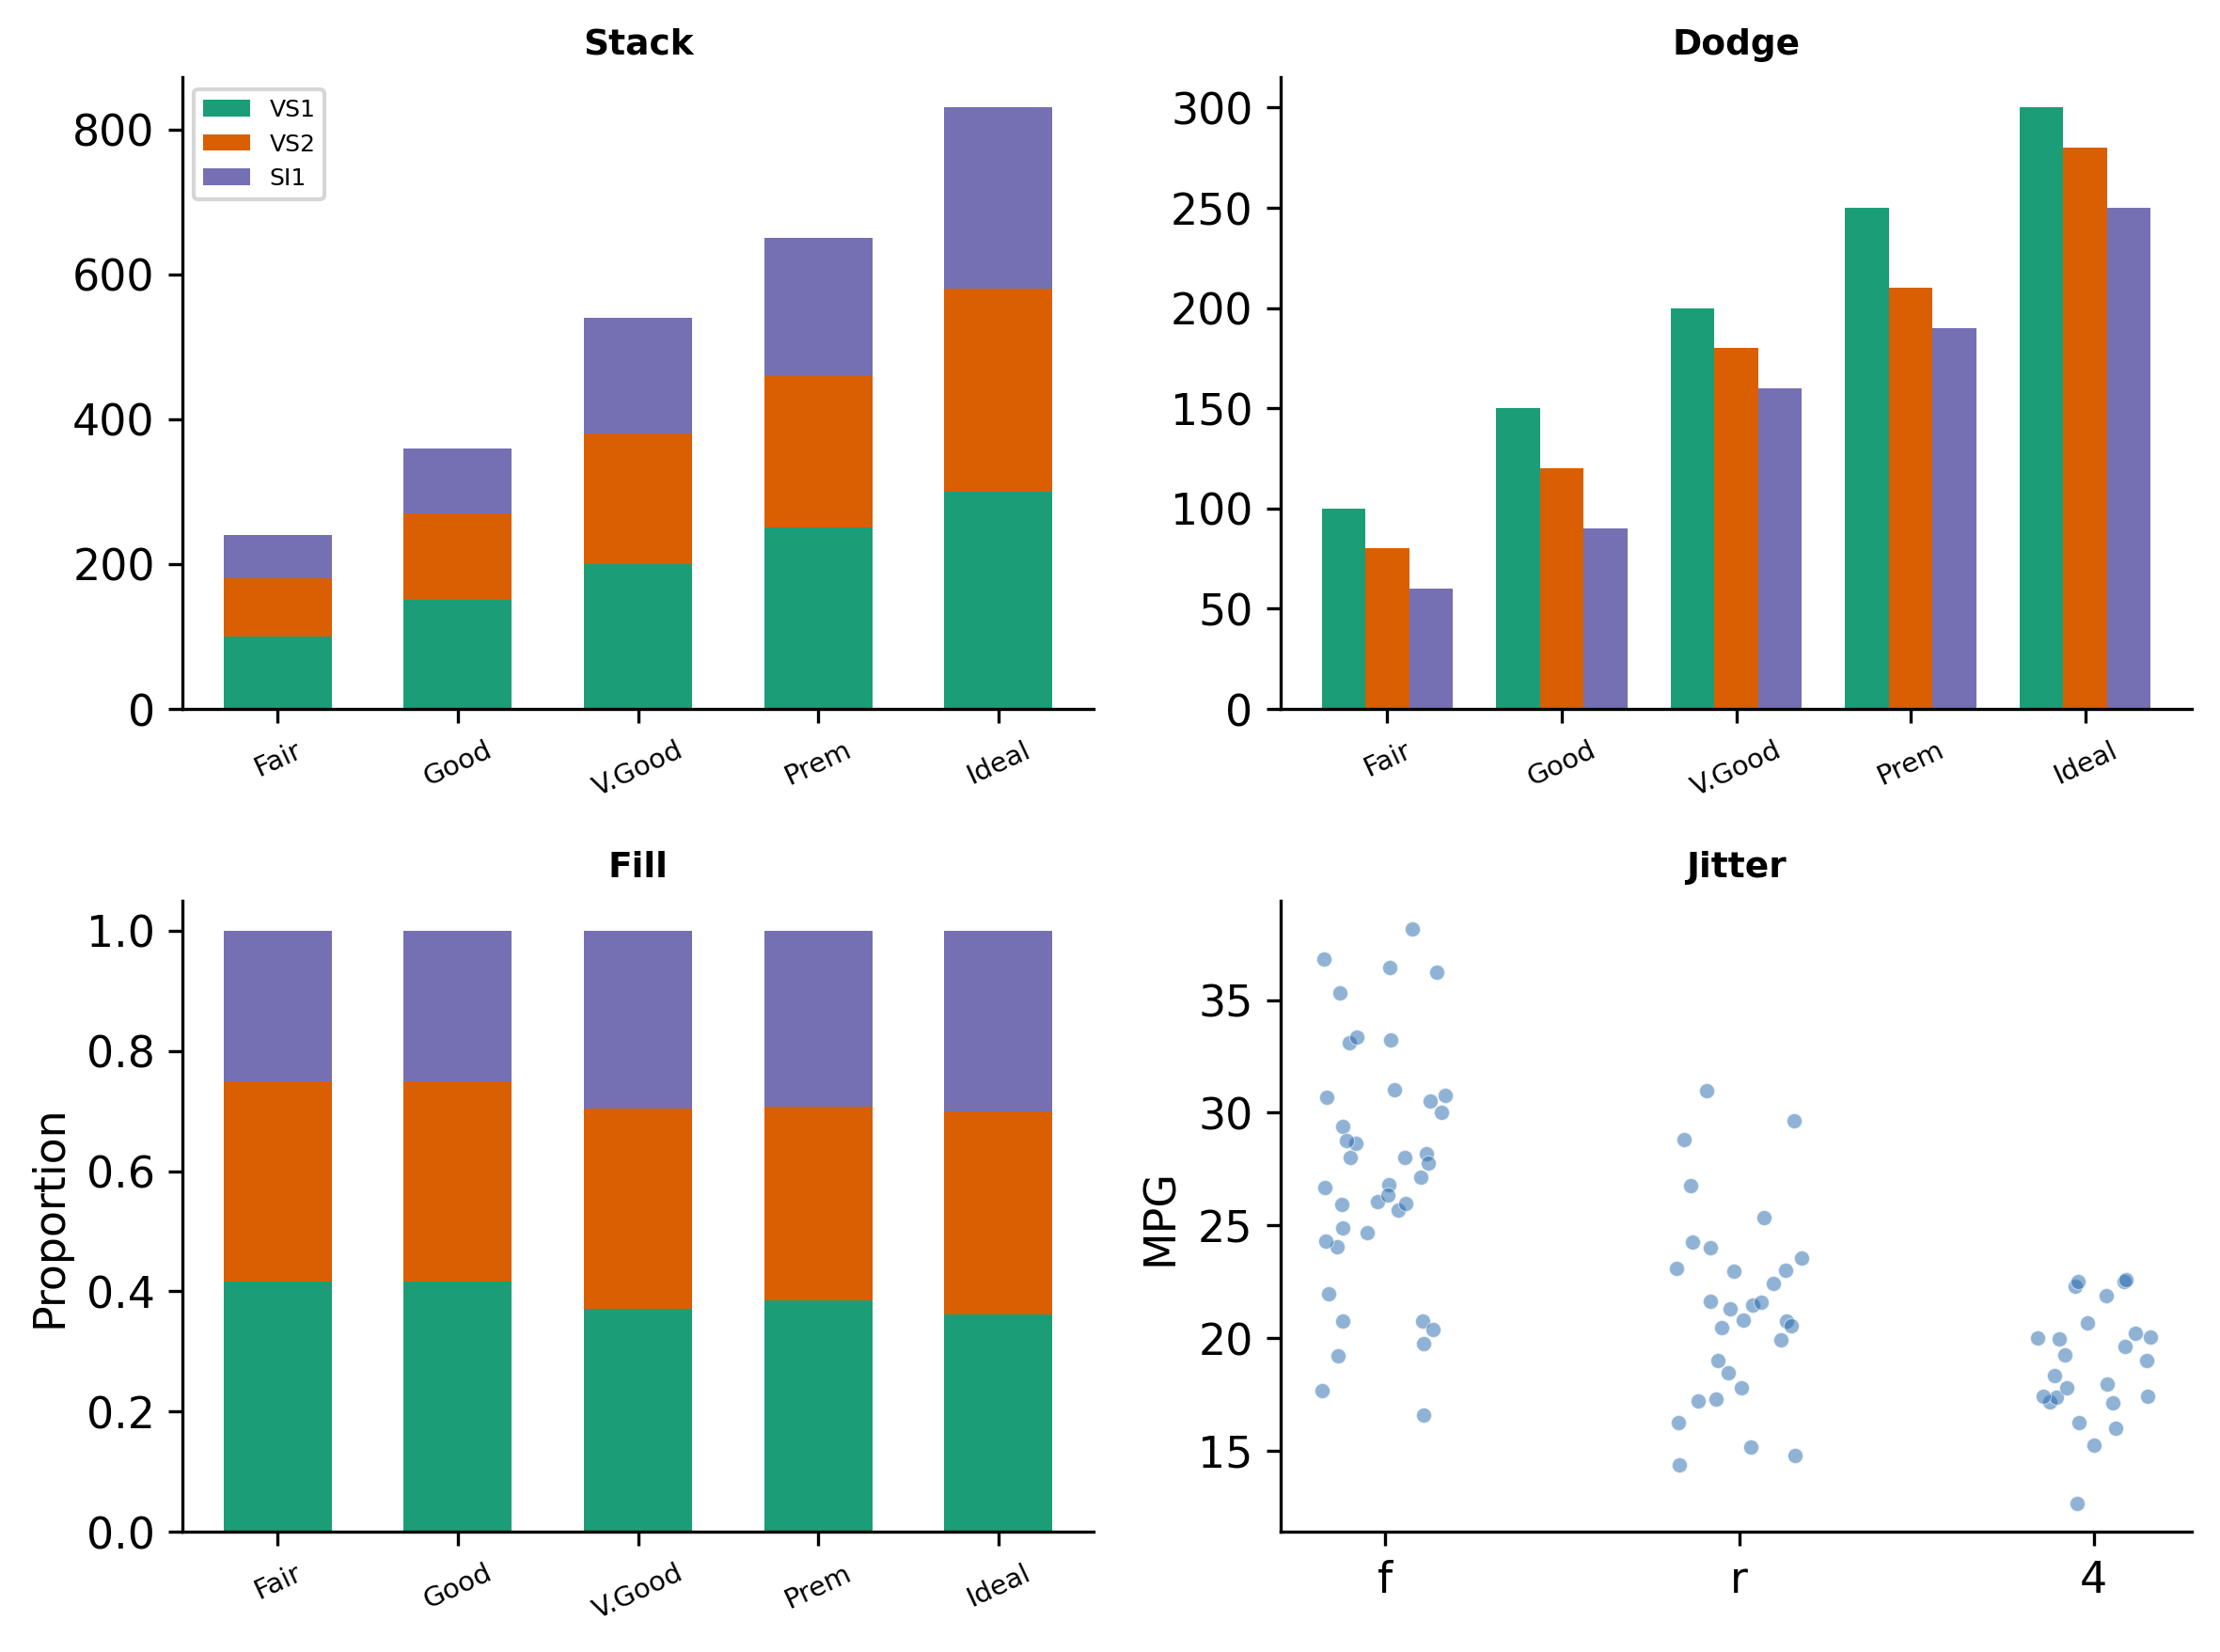
\includegraphics[width=0.9\textwidth]{m1_3_positions.png}
\end{column}
\begin{column}{0.48\textwidth}
\begin{lstlisting}[style=Rstyle]
# Dodged (side by side)
ggplot(diamonds,
  aes(cut, fill=clarity)) +
  geom_bar(position="dodge")
\end{lstlisting}
\centering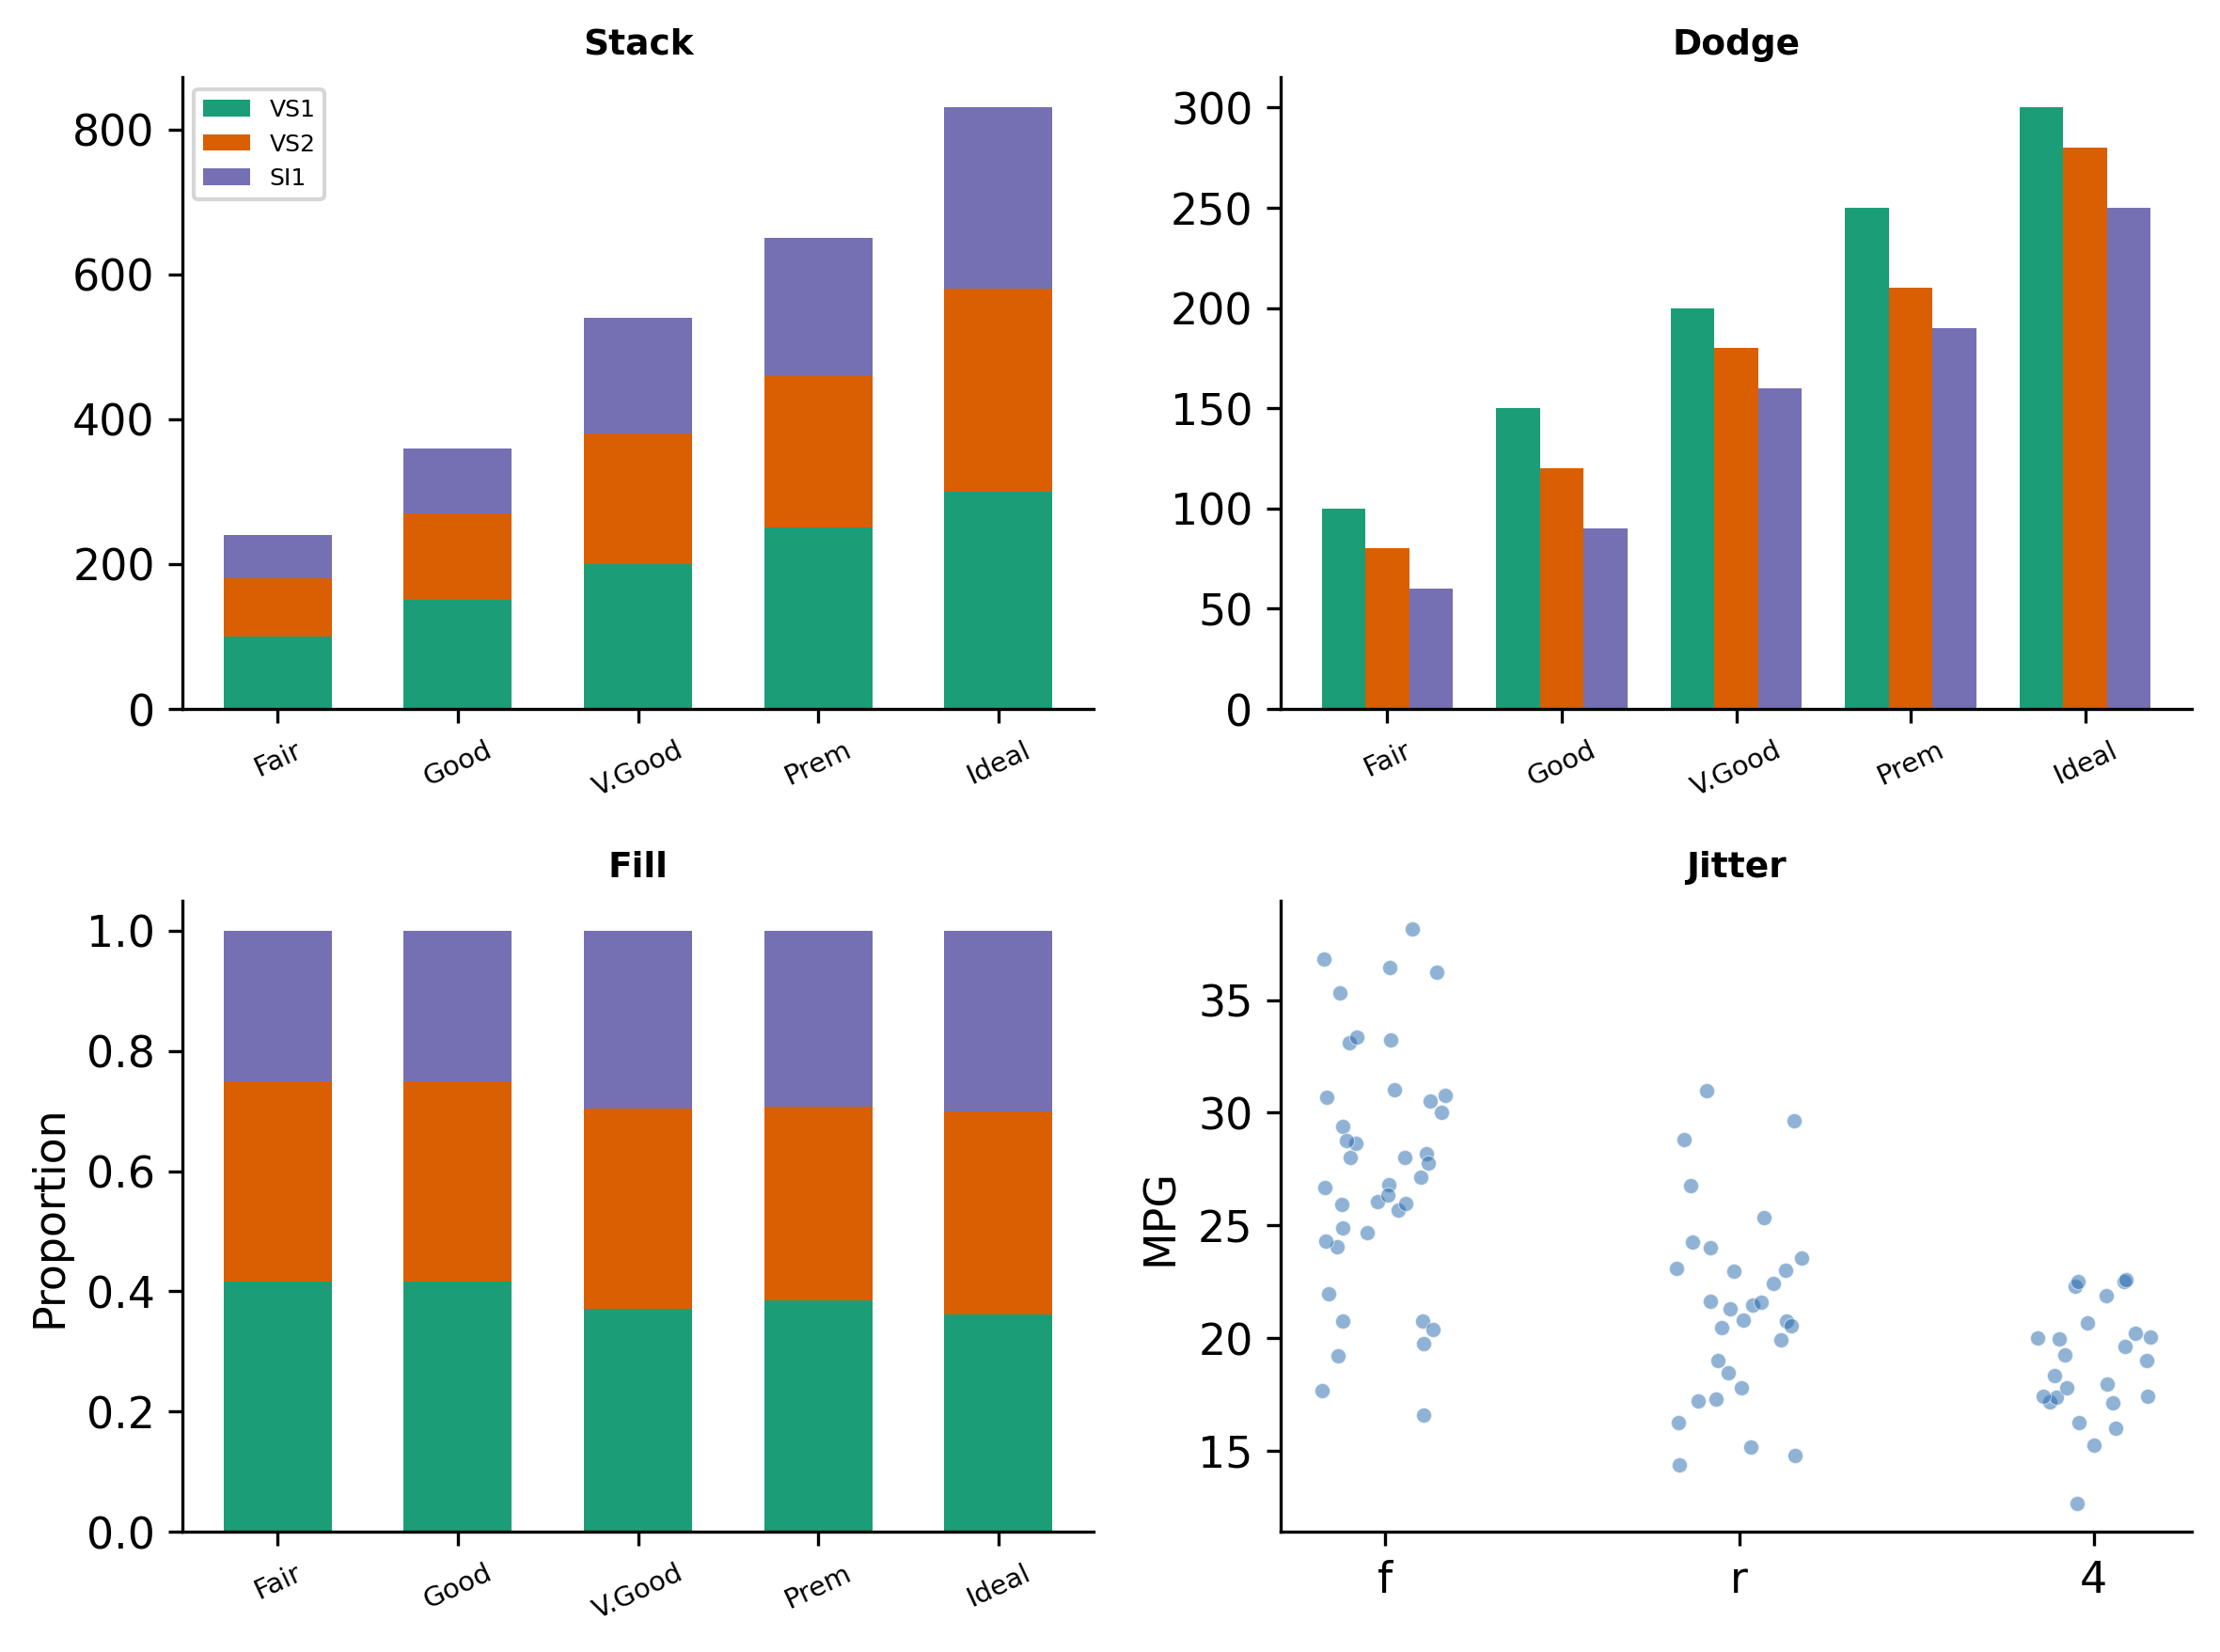
\includegraphics[width=0.9\textwidth]{m1_3_positions.png}
\end{column}
\end{columns}
\scriptref{scripts/m1\_3\_positions.R}
\end{frame}

% ── 80 ──
\begin{frame}[fragile]{Position: Fill and Jitter --- \Rlang}\smark{80/300}
\begin{columns}[T]
\begin{column}{0.48\textwidth}
\begin{lstlisting}[style=Rstyle]
# Percent-stacked
ggplot(diamonds,
  aes(cut, fill=clarity)) +
  geom_bar(position="fill") +
  labs(y = "proportion")
\end{lstlisting}
\centering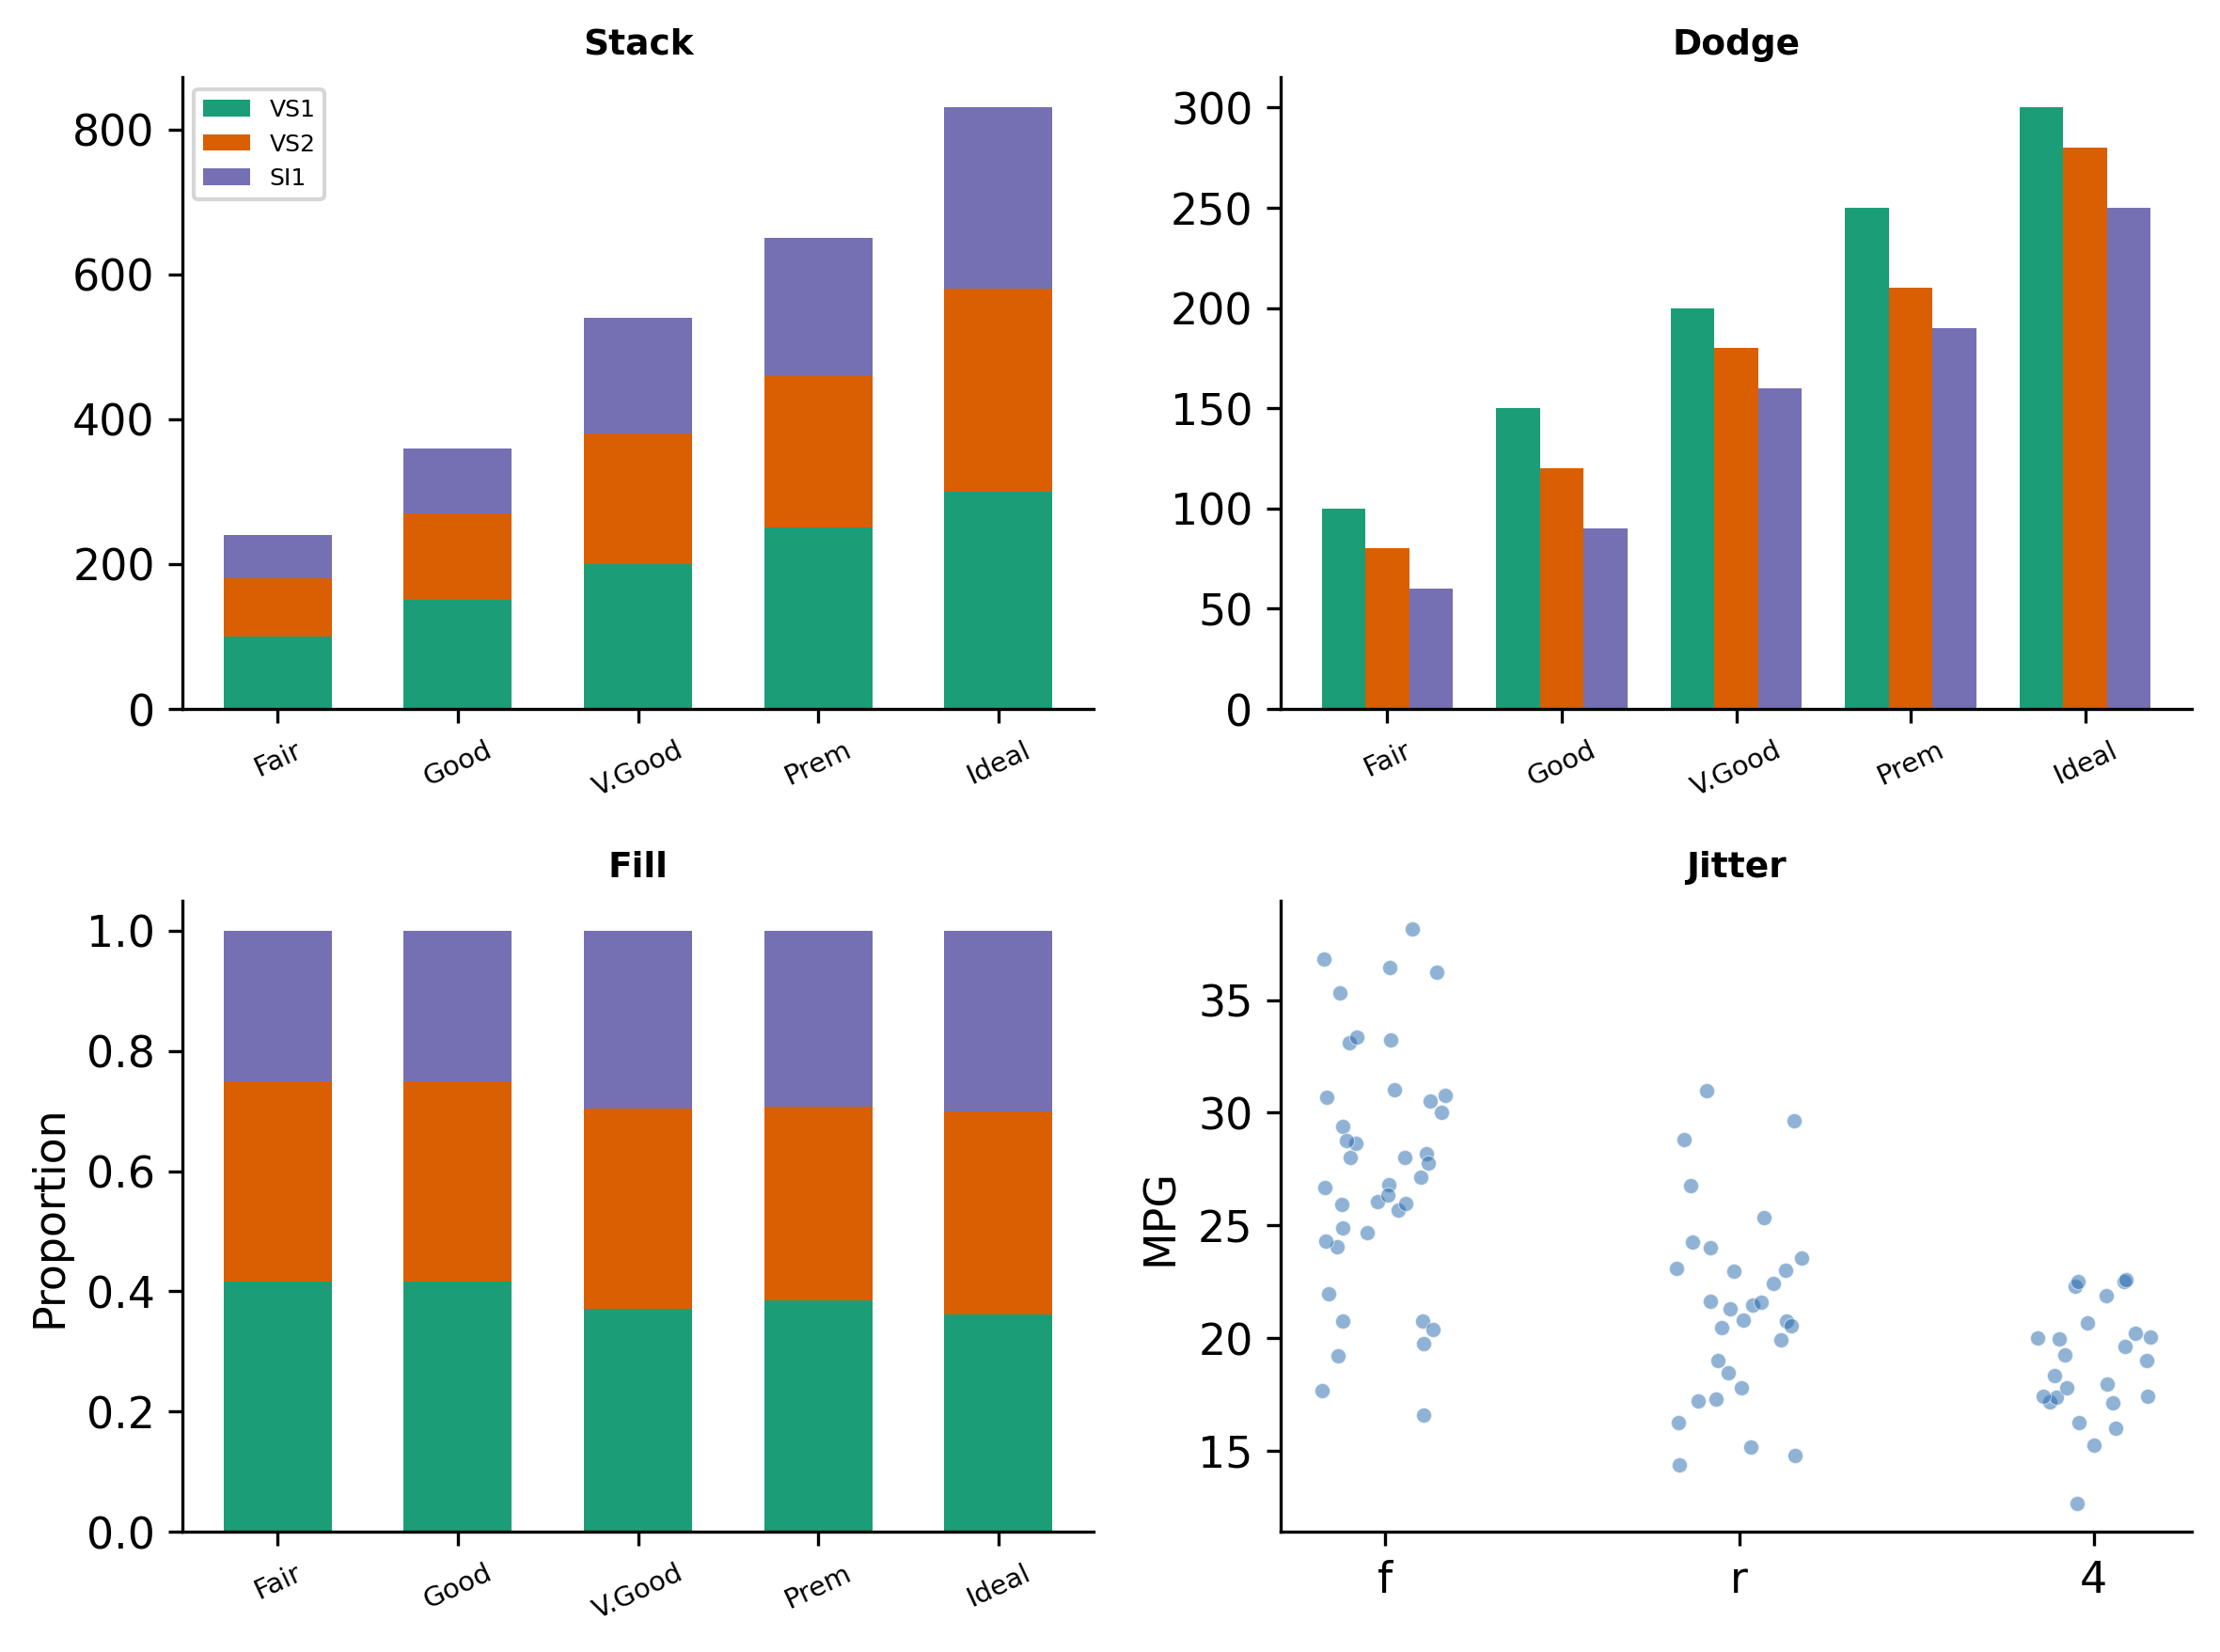
\includegraphics[width=0.9\textwidth]{m1_3_positions.png}
\end{column}
\begin{column}{0.48\textwidth}
\begin{lstlisting}[style=Rstyle]
# Jitter for categorical x
ggplot(mpg, aes(drv, hwy)) +
  geom_jitter(width=0.2,
              alpha=0.5,
              color="#2166AC")
\end{lstlisting}
\centering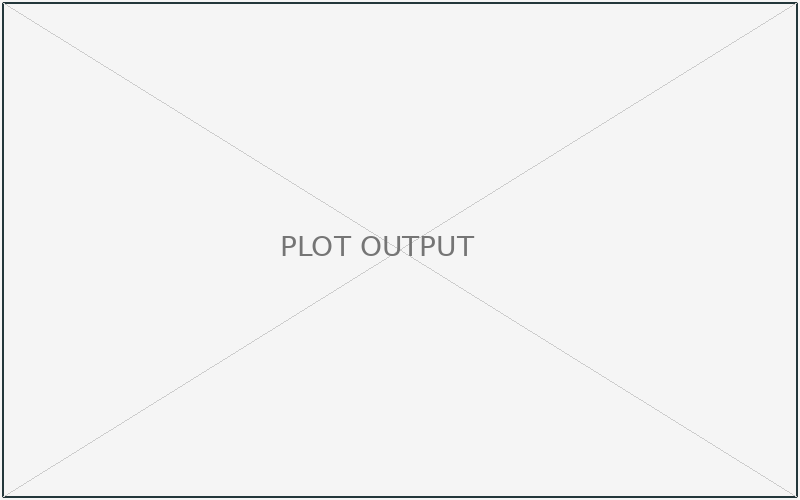
\includegraphics[width=0.9\textwidth]{placeholder.png}
\end{column}
\end{columns}
\scriptref{scripts/m1\_3\_positions.R}
\end{frame}

% ── 81 ──
\begin{frame}[fragile]{Position Adjustments --- \Python}\smark{81/300}
\begin{columns}[T]
\begin{column}{0.55\textwidth}
\begin{lstlisting}[style=Pystyle]
# plotnine: identical syntax
(ggplot(diamonds,
   aes("cut", fill="clarity"))
 + geom_bar(position="dodge"))

# seaborn: hue parameter
sns.countplot(data=diamonds,
    x="cut", hue="clarity")

# Jitter in plotnine
(ggplot(mpg, aes("drv","hwy"))
 + geom_jitter(width=0.2,
               alpha=0.5))
\end{lstlisting}
\scriptref{scripts/m1\_3\_positions.py}
\end{column}
\begin{column}{0.42\textwidth}
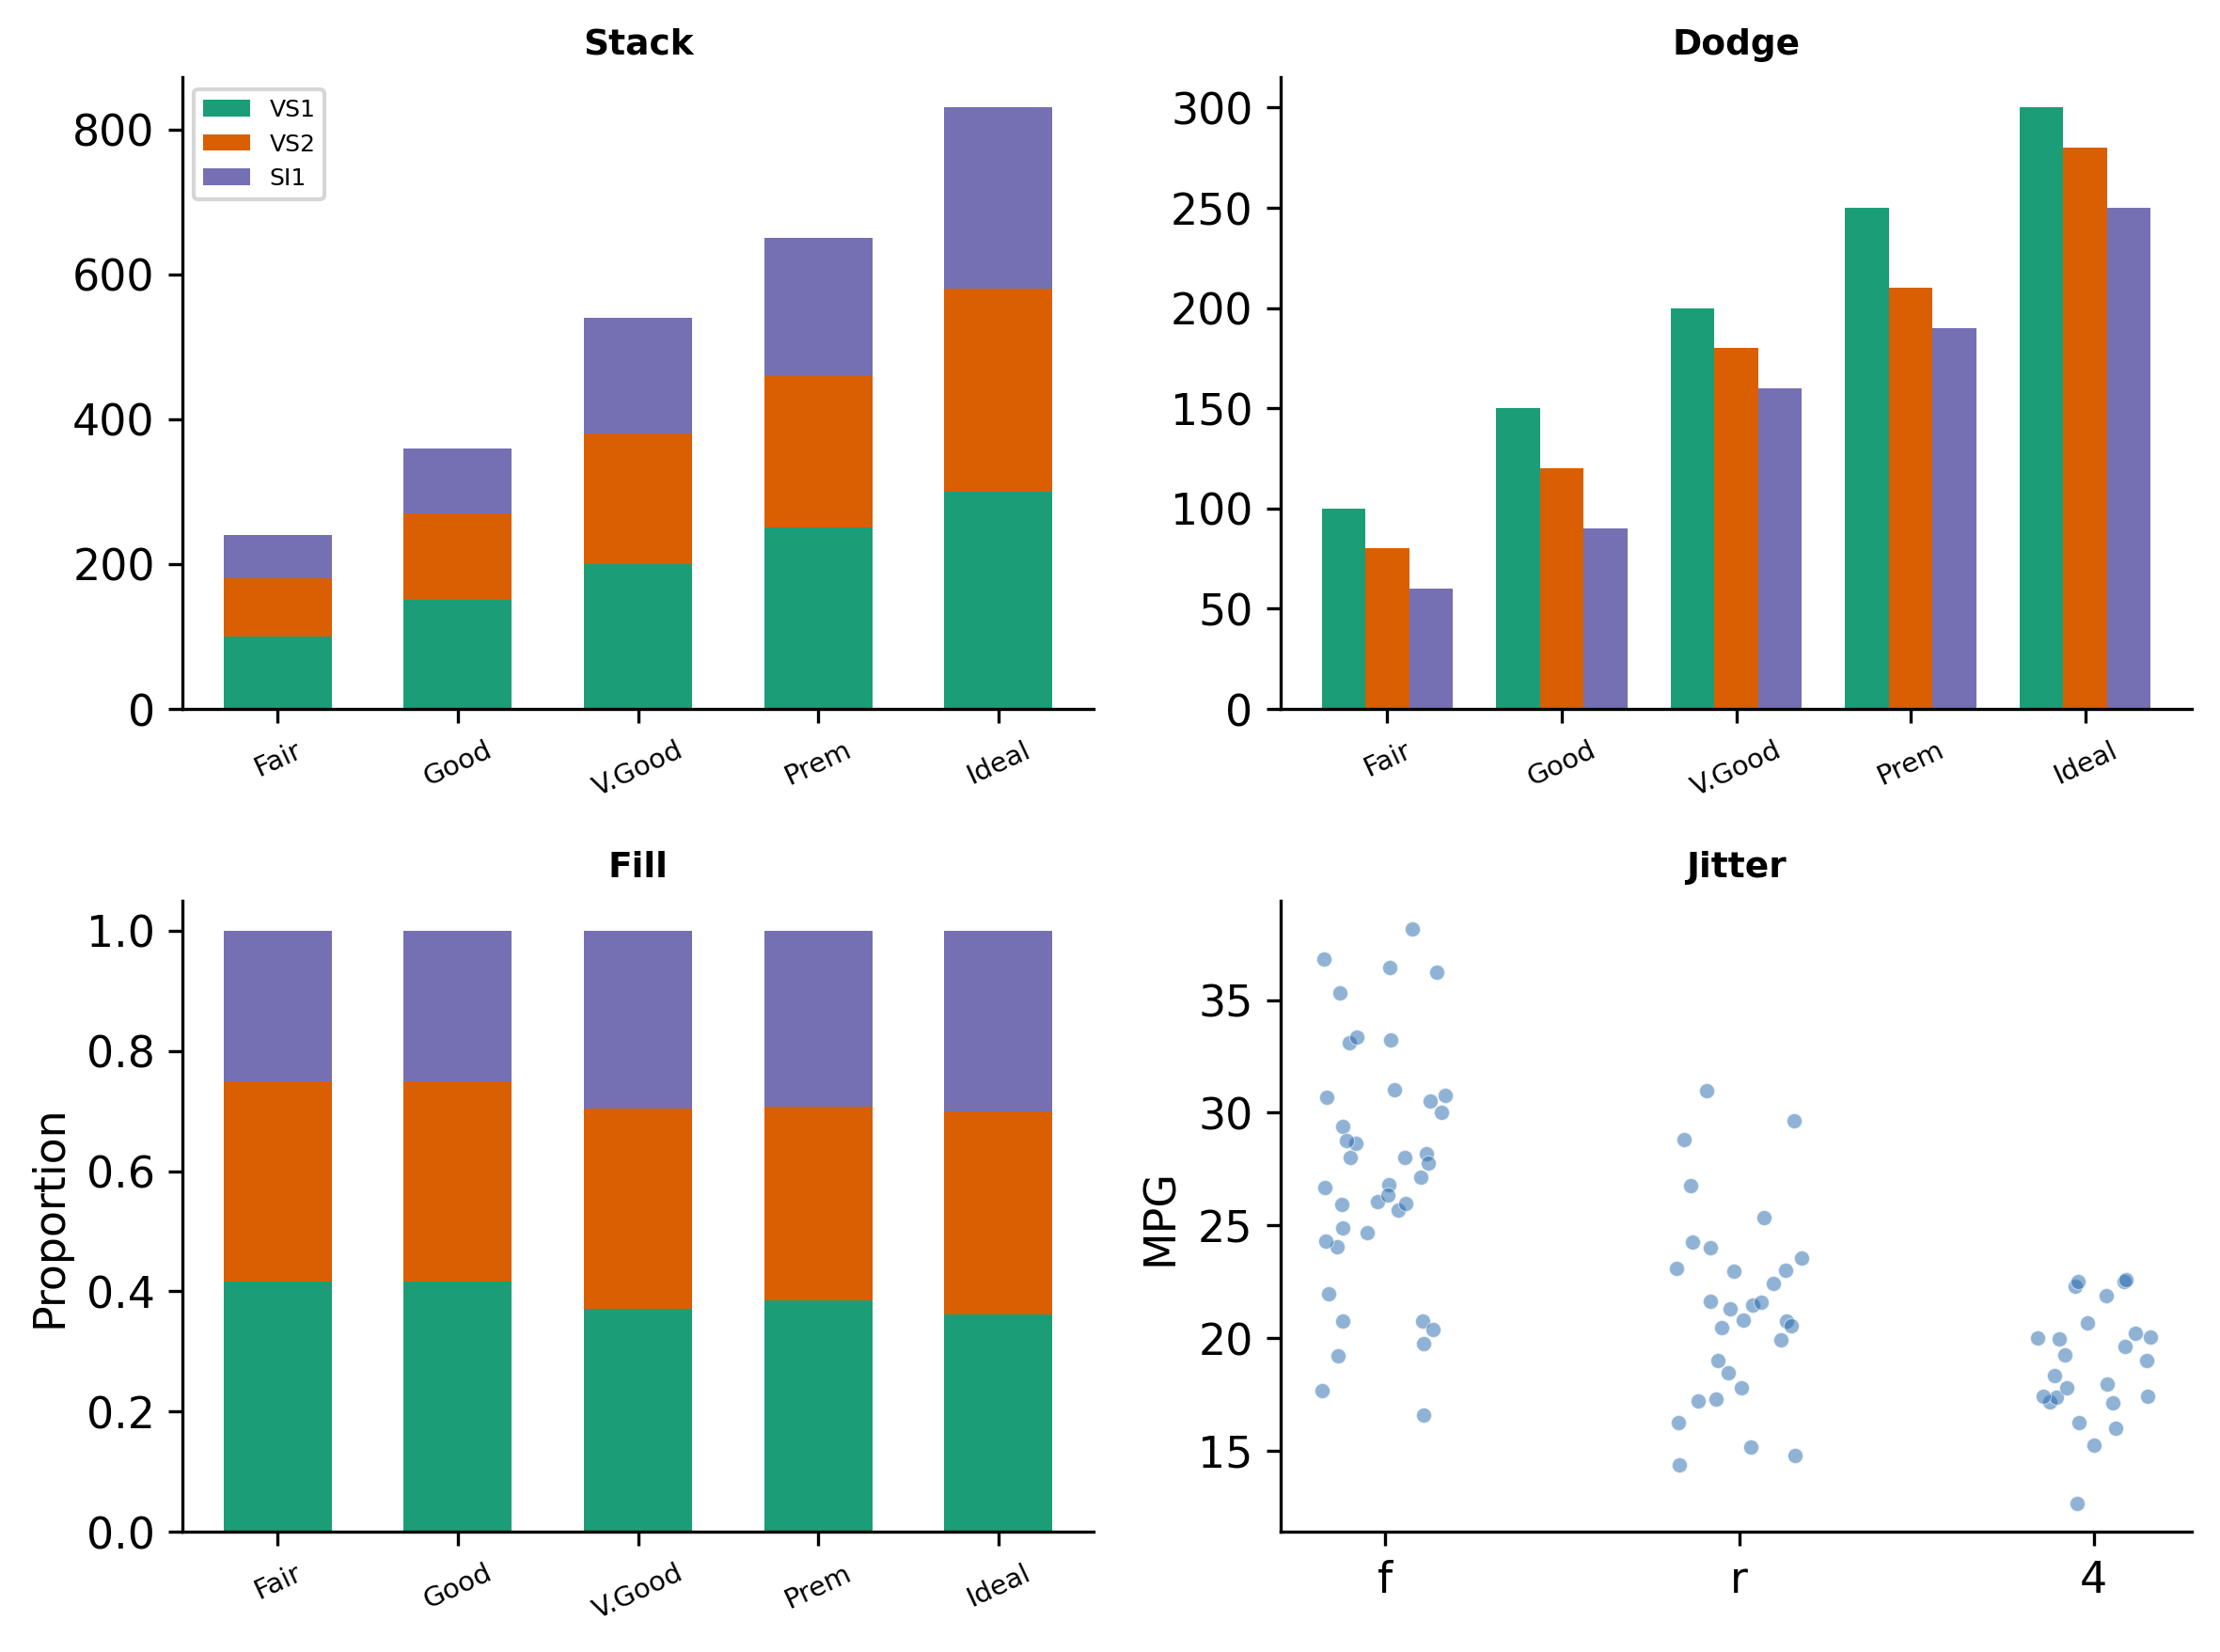
\includegraphics[width=\textwidth]{m1_3_positions.png}
\begin{alertblock}{Pro-Tip}
    \scriptsize In seaborn, \texttt{hue} creates grouped bars automatically. In plotnine, use \texttt{position="dodge"} explicitly.
\end{alertblock}
\end{column}
\end{columns}
\end{frame}

% ── 82 ──
\begin{frame}{The Line Chart: When and Why}
\smark{82/300}
\begin{columns}[T]
\begin{column}{0.50\textwidth}
\begin{itemize}
    \item Shows \textbf{trend over an ordered} variable (usually time)
    \item Exploits Gestalt \textbf{continuity} --- the eye follows the line
    \item Implies interpolation between observed points
    \item Never use for unordered categories
\end{itemize}
\end{column}
\begin{column}{0.47\textwidth}
\begin{exampleblock}{Data Insight}
    \scriptsize A line says ``the value changed \emph{continuously} between observations.'' If that isn't true (e.g., survey waves), use points connected by segments.
\end{exampleblock}
\end{column}
\end{columns}
\end{frame}

% ── 83 ──
\begin{frame}[fragile]{Basic Line Chart --- \Rlang}\smark{83/300}
\begin{columns}[T]
\begin{column}{0.55\textwidth}
\begin{lstlisting}[style=Rstyle]
ggplot(economics,
  aes(date, unemploy / 1000)) +
  geom_line(color = "#2166AC",
            linewidth = 0.6) +
  labs(x = NULL,
       y = "Unemployed (millions)",
       title = "US Unemployment") +
  theme_minimal()
\end{lstlisting}
\scriptref{scripts/m1\_3\_line\_basic.R}
\end{column}
\begin{column}{0.42\textwidth}
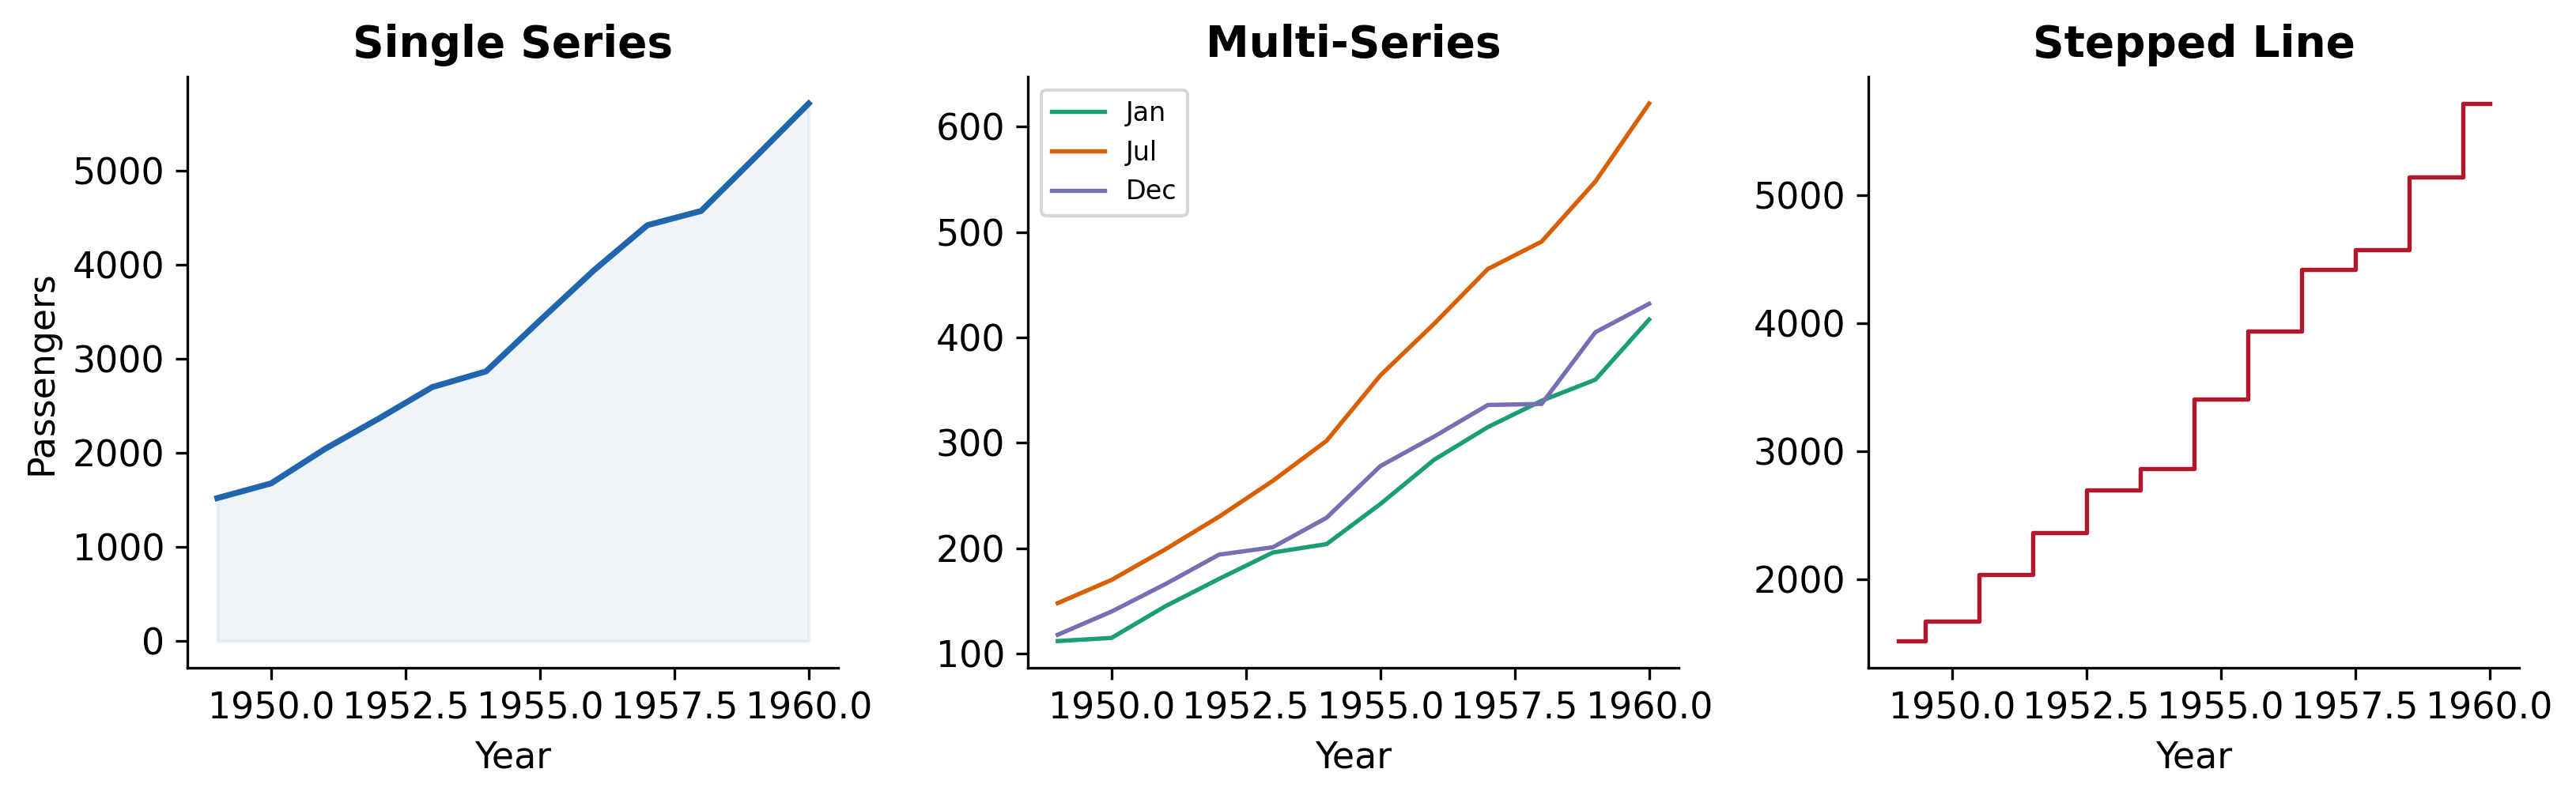
\includegraphics[width=\textwidth]{m1_3_lines.png}
\begin{exampleblock}{Data Insight}
    \scriptsize Recessions visible as sharp upward spikes. The line encodes both \emph{level} and \emph{rate of change} (slope).
\end{exampleblock}
\end{column}
\end{columns}
\end{frame}

% ── 84 ──
\begin{frame}[fragile]{Basic Line Chart --- \Python}\smark{84/300}
\begin{columns}[T]
\begin{column}{0.55\textwidth}
\begin{lstlisting}[style=Pystyle]
flights = sns.load_dataset("flights")
total = (flights.groupby("year")
         ["passengers"].sum()
         .reset_index())

plt.plot(total["year"],
         total["passengers"],
         color="#B2182B",
         linewidth=1.2)
plt.xlabel("Year")
plt.ylabel("Total Passengers")
\end{lstlisting}
\scriptref{scripts/m1\_3\_line\_basic.py}
\end{column}
\begin{column}{0.42\textwidth}
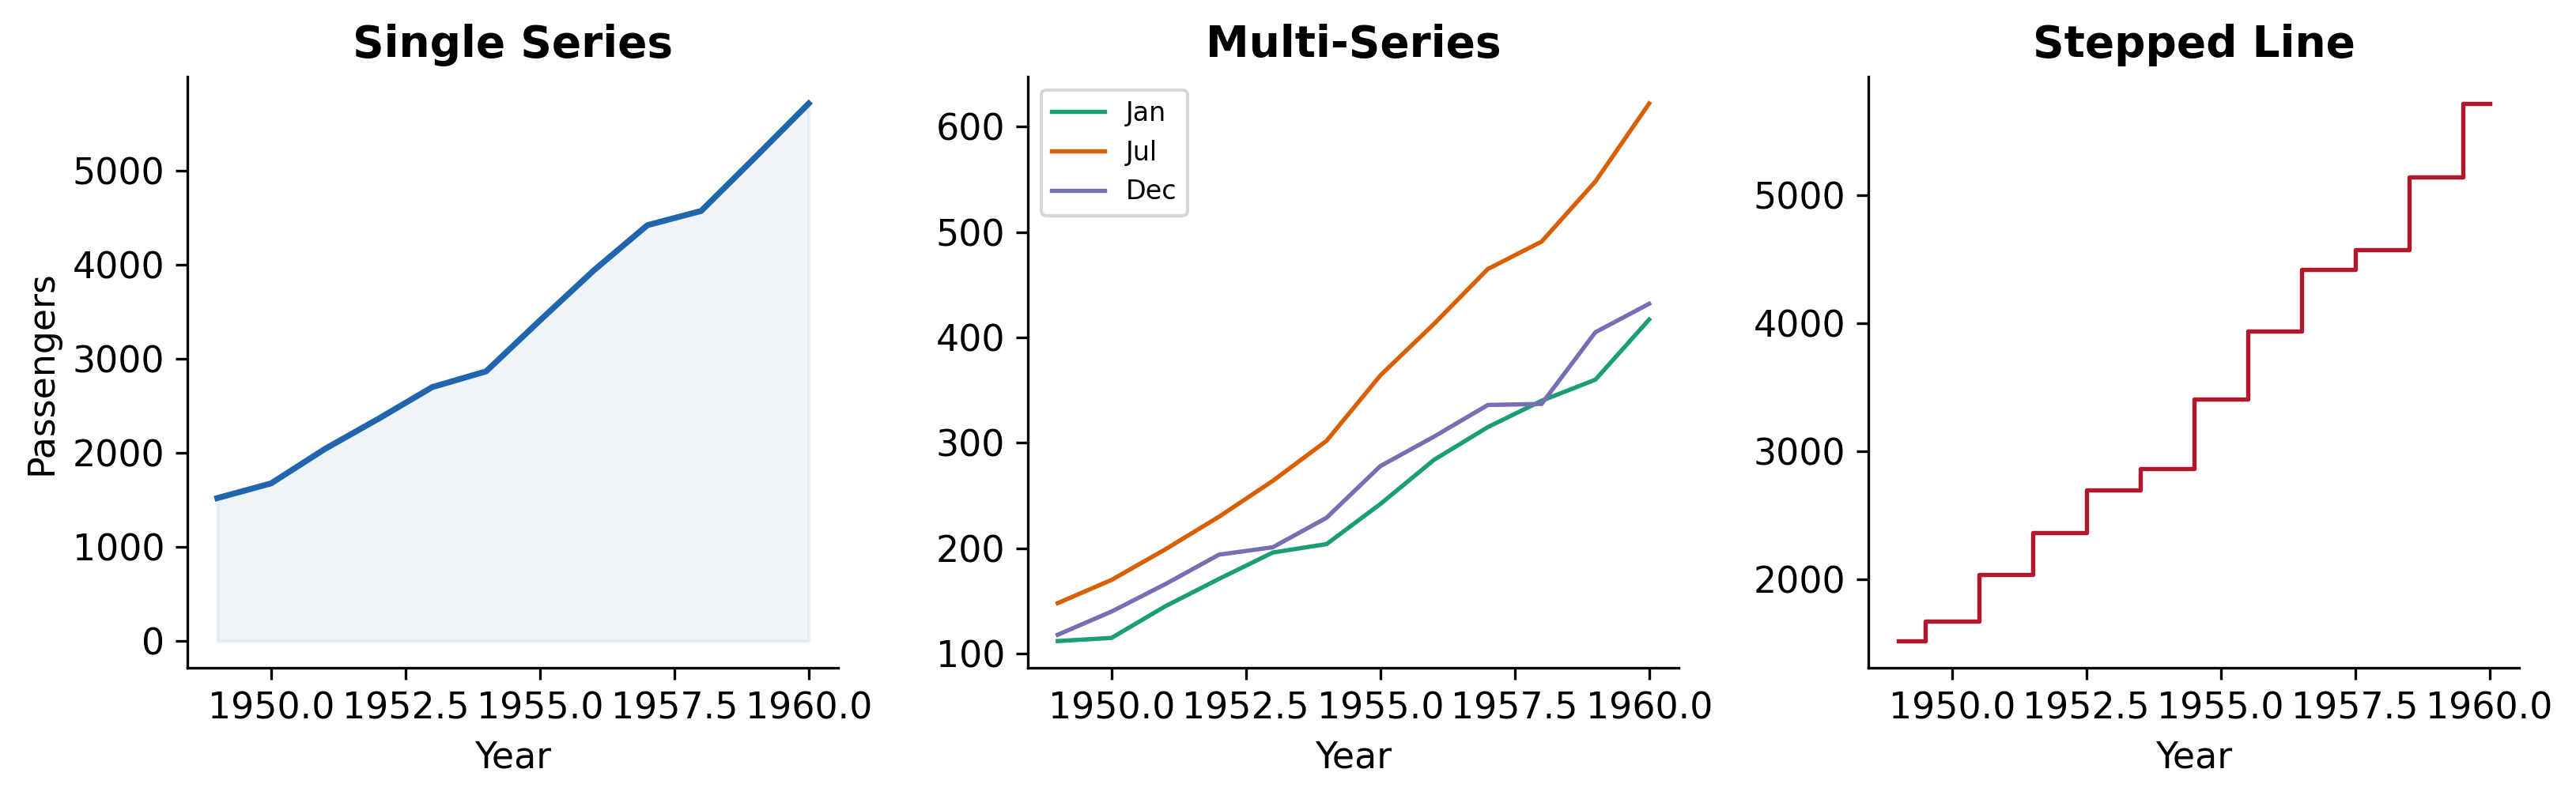
\includegraphics[width=\textwidth]{m1_3_lines.png}
\begin{alertblock}{Pro-Tip}
    \scriptsize \texttt{plt.plot()} draws lines by default. For scatter, use \texttt{plt.scatter()}.
\end{alertblock}
\end{column}
\end{columns}
\end{frame}

% ── 85 ──
\begin{frame}[fragile]{Multi-Series Lines --- \Rlang}\smark{85/300}
\begin{columns}[T]
\begin{column}{0.55\textwidth}
\begin{lstlisting}[style=Rstyle]
el <- economics_long |>
  filter(variable %in%
    c("psavert","uempmed"))

ggplot(el,
  aes(date, value,
      color = variable)) +
  geom_line(linewidth = 0.5) +
  labs(x=NULL, y="Value",
       color="Indicator") +
  theme_minimal()
\end{lstlisting}
\end{column}
\begin{column}{0.42\textwidth}
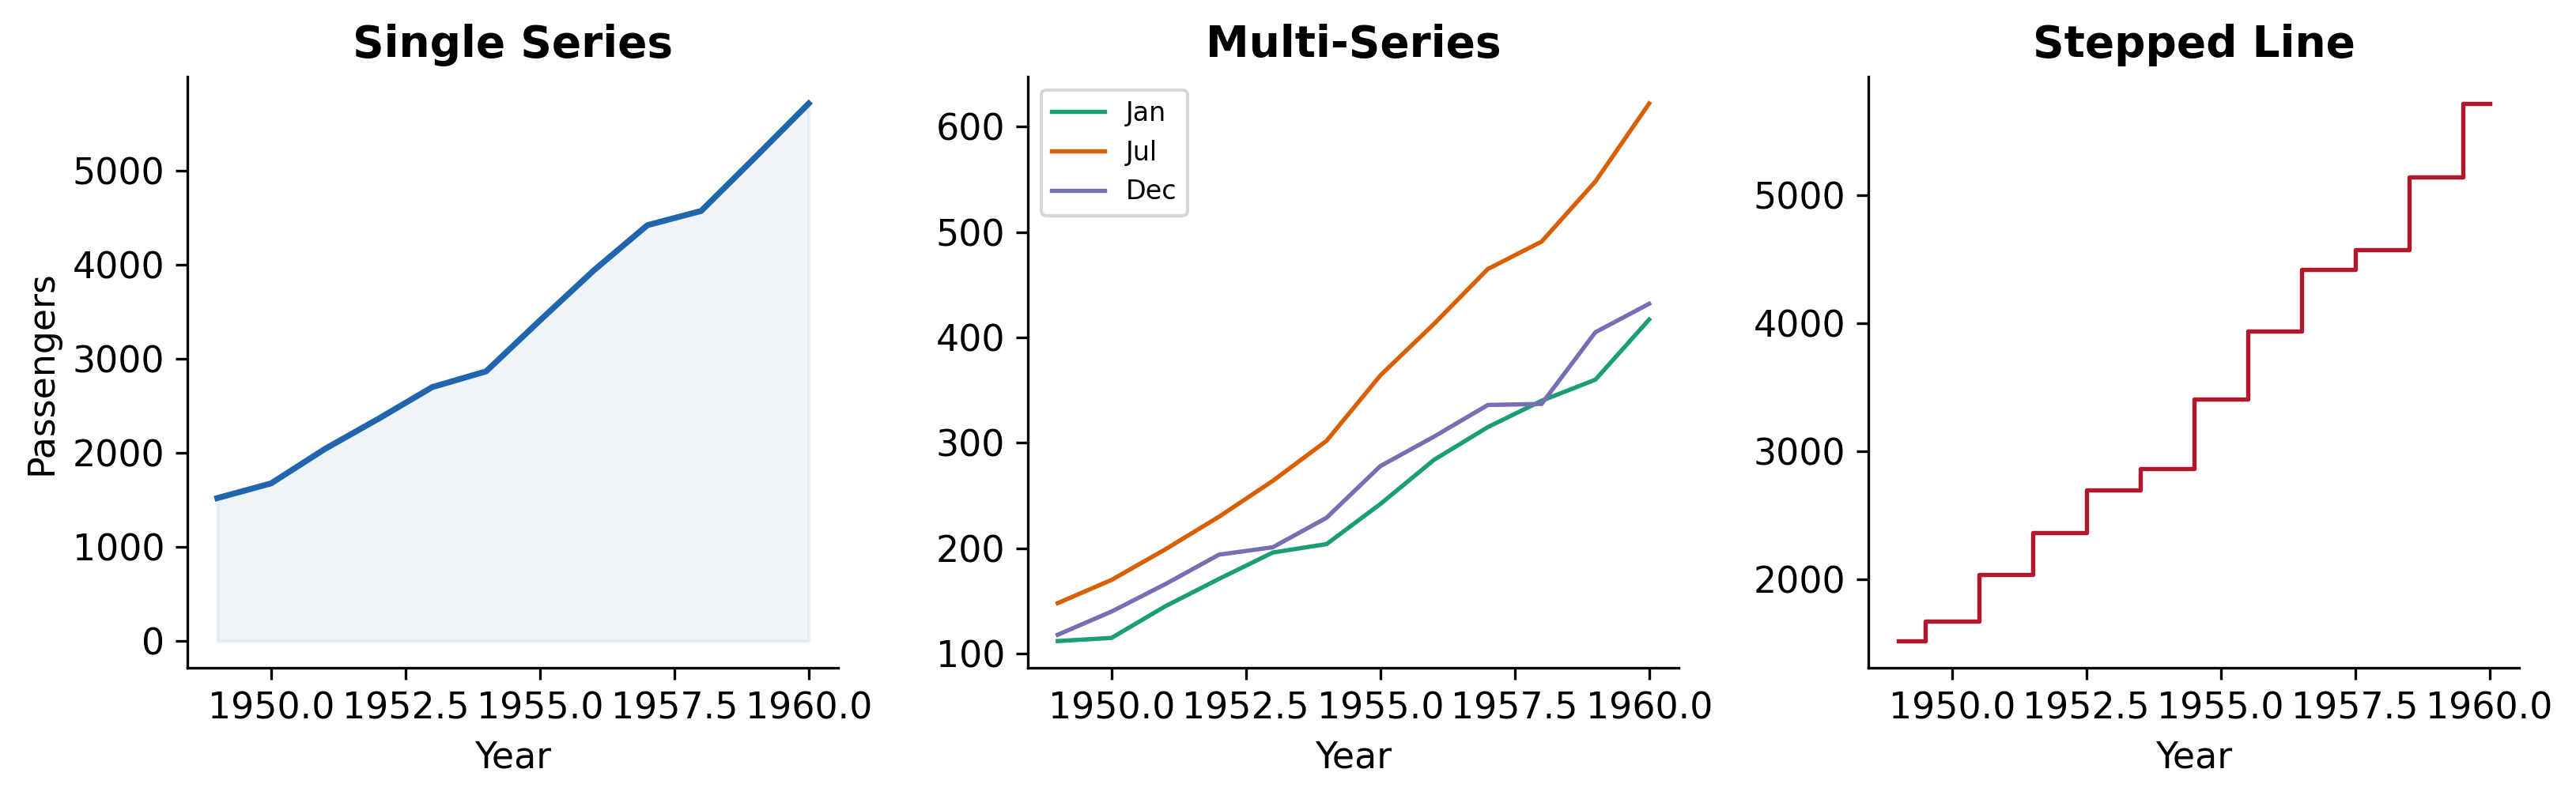
\includegraphics[width=\textwidth]{m1_3_lines.png}
\begin{exampleblock}{Data Insight}
    \scriptsize Multi-series lines need the \textbf{color} aesthetic so ggplot knows which points to connect.
\end{exampleblock}
\end{column}
\end{columns}
\end{frame}

% ── 86 ──
\begin{frame}[fragile]{Multi-Series Lines --- \Python}\smark{86/300}
\begin{columns}[T]
\begin{column}{0.55\textwidth}
\begin{lstlisting}[style=Pystyle]
flights = sns.load_dataset("flights")

for month in ["Jan","Jul","Dec"]:
    sub = flights[
        flights["month"] == month]
    plt.plot(sub["year"],
             sub["passengers"],
             label=month)
plt.legend()
plt.xlabel("Year")
\end{lstlisting}
\scriptref{scripts/m1\_3\_line\_basic.py}
\end{column}
\begin{column}{0.42\textwidth}
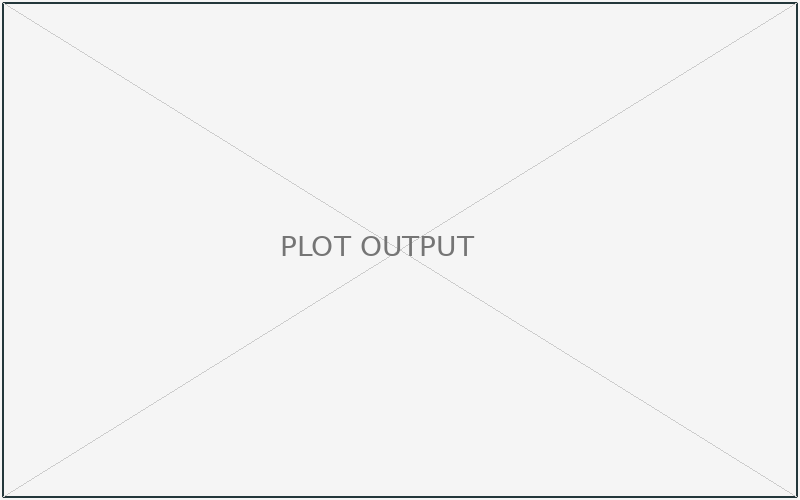
\includegraphics[width=\textwidth]{placeholder.png}
\begin{alertblock}{Pro-Tip}
    \scriptsize In matplotlib, each \texttt{plot()} adds a series. In ggplot2/plotnine, one call + \texttt{color=variable} handles all.
\end{alertblock}
\end{column}
\end{columns}
\end{frame}

% ── 87 ──
\begin{frame}[fragile]{Stepped Lines and Missing Data}
\smark{87/300}
\begin{columns}[T]
\begin{column}{0.50\textwidth}
\textbf{Stepped lines} (\texttt{geom\_step}):
\begin{itemize}
    \item Value held constant until next change
    \item Interest rates, discrete prices
    \item No interpolation assumption
\end{itemize}
\vspace{0.2cm}
\textbf{Missing data gaps}:
\begin{itemize}
    \item \texttt{geom\_line()} skips \texttt{NA} (gap)
    \item Connecting across gaps = false continuity
    \item Show gaps honestly
\end{itemize}
\end{column}
\begin{column}{0.47\textwidth}
\begin{lstlisting}[style=Rstyle]
# Stepped line
ggplot(economics,
  aes(date, uempmed)) +
  geom_step(color="#B2182B")

# NA creates gap in line
df$y[5:8] <- NA
ggplot(df, aes(x, y)) +
  geom_line()
\end{lstlisting}
\begin{alertblock}{Pro-Tip}
    \scriptsize \texttt{geom\_step()} for piecewise-constant data. \texttt{NA} preserves honest gaps in \texttt{geom\_line()}.
\end{alertblock}
\end{column}
\end{columns}
\end{frame}

% ── 88 ──
\begin{frame}{Choosing Scatter vs.\ Bar vs.\ Line}
\smark{88/300}
\centering\small
\begin{tabular}{@{}l l l l@{}}
    \toprule
    \textbf{X variable} & \textbf{Y variable} & \textbf{Task} & \textbf{Geom} \\
    \midrule
    Continuous  & Continuous  & Relationship    & \texttt{geom\_point} \\
    Categorical & Continuous  & Compare groups  & \texttt{geom\_col} \\
    Ordered/Time& Continuous  & Trend           & \texttt{geom\_line} \\
    Categorical & Count       & Frequency       & \texttt{geom\_bar} \\
    Categorical & Categorical & Association     & Module 3 \\
    \bottomrule
\end{tabular}

\vspace{0.3cm}
\begin{exampleblock}{Data Insight}
    \scriptsize This decision table covers $\sim$80\% of everyday plots. Modules 1.4--1.10 add the remaining 20\%.
\end{exampleblock}
\end{frame}

% ── 89 ──
\begin{frame}{Module 1.3 --- Key Takeaways}\smark{89/300}
\begin{enumerate}
    \item \textbf{Scatter = two continuous variables.} Add color/size/shape for more.
    \item \textbf{Diagnose overplotting early.} Alpha, jitter, density are your tools.
    \item \textbf{Bars start at zero.} Always. Sort by value unless order is intrinsic.
    \item \textbf{Position adjustments} control grouped geoms: stack, dodge, fill.
    \item \textbf{Lines imply continuity.} Only connect ordered observations.
\end{enumerate}
\end{frame}

% ── 90 ──
\begin{frame}{}\smark{90/300}
\centering\vspace{1.5cm}
{\Large\textbf{Module 1.3 Complete}}\\[0.5cm]
You can now build the three workhorse geoms --- scatter, bar, and line --- with multi-variable encodings and position adjustments.\\[0.5cm]
\textbf{Next:} Module 1.4 --- Histograms, Density, and Distribution Shape.
\end{frame}

% ═══════════════════════════════════════════════════════
%  MODULE 1.4 — Histograms, Density, and Distribution Shape
% ═══════════════════════════════════════════════════════
\section{Module 1.4 --- Histograms, Density, and Distribution Shape}

% ── 91 ──
\begin{frame}{Module 1.4 --- Roadmap}\smark{91/300}
\begin{enumerate}
    \item The histogram: binning continuous data
    \item Binwidth sensitivity and the Freedman--Diaconis rule
    \item Frequency polygons as line-based alternatives
    \item Kernel Density Estimation (KDE): theory and bandwidth
    \item Histogram + density + rug overlay
    \item Grouped and stacked histograms
    \item QQ plots for distributional assessment
    \item Faceted distributions across groups
\end{enumerate}
\end{frame}

% ── 92 ──
\begin{frame}{Why Distributions Matter}\smark{92/300}
\begin{columns}[T]
\begin{column}{0.50\textwidth}
\begin{itemize}
    \item Summary stats ($\bar{x}$, $s$) hide \textbf{shape}: skew, bimodality, outliers
    \item Distributions inform \textbf{model choice}: normal $\to$ $t$-test; skewed $\to$ non-parametric
    \item Visualization is the \textbf{first test of normality} --- faster than Shapiro--Wilk
\end{itemize}
\end{column}
\begin{column}{0.47\textwidth}
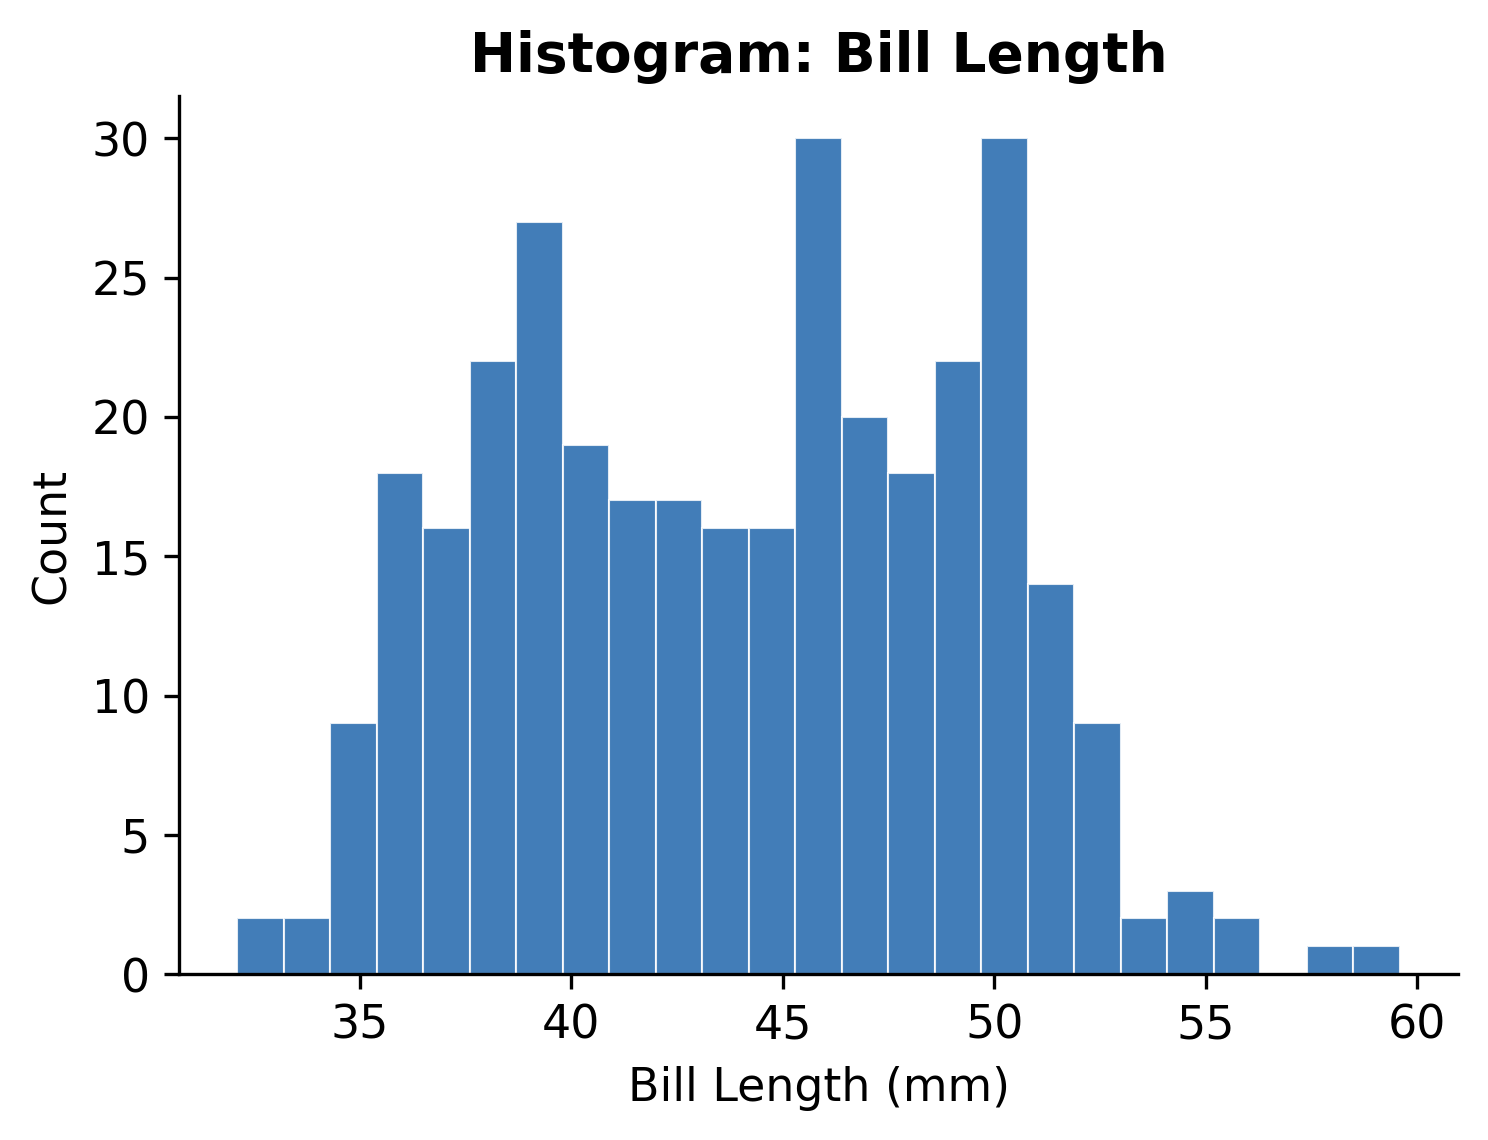
\includegraphics[width=\textwidth]{m1_4_hist_basic.png}
\begin{exampleblock}{Data Insight}
    \scriptsize The bimodal shape here suggests two sub-populations. A mean of 44\,mm would describe neither peak accurately.
\end{exampleblock}
\end{column}
\end{columns}
\end{frame}

% ── 93 ──
\begin{frame}[fragile]{Basic Histogram --- \Rlang}\smark{93/300}
\begin{columns}[T]
\begin{column}{0.55\textwidth}
\begin{lstlisting}[style=Rstyle]
library(palmerpenguins)

ggplot(penguins,
  aes(x = bill_length_mm)) +
  geom_histogram(bins = 25,
    fill = "#2166AC",
    color = "white") +
  labs(x = "Bill Length (mm)",
       y = "Count") +
  theme_minimal()
\end{lstlisting}
\end{column}
\begin{column}{0.42\textwidth}
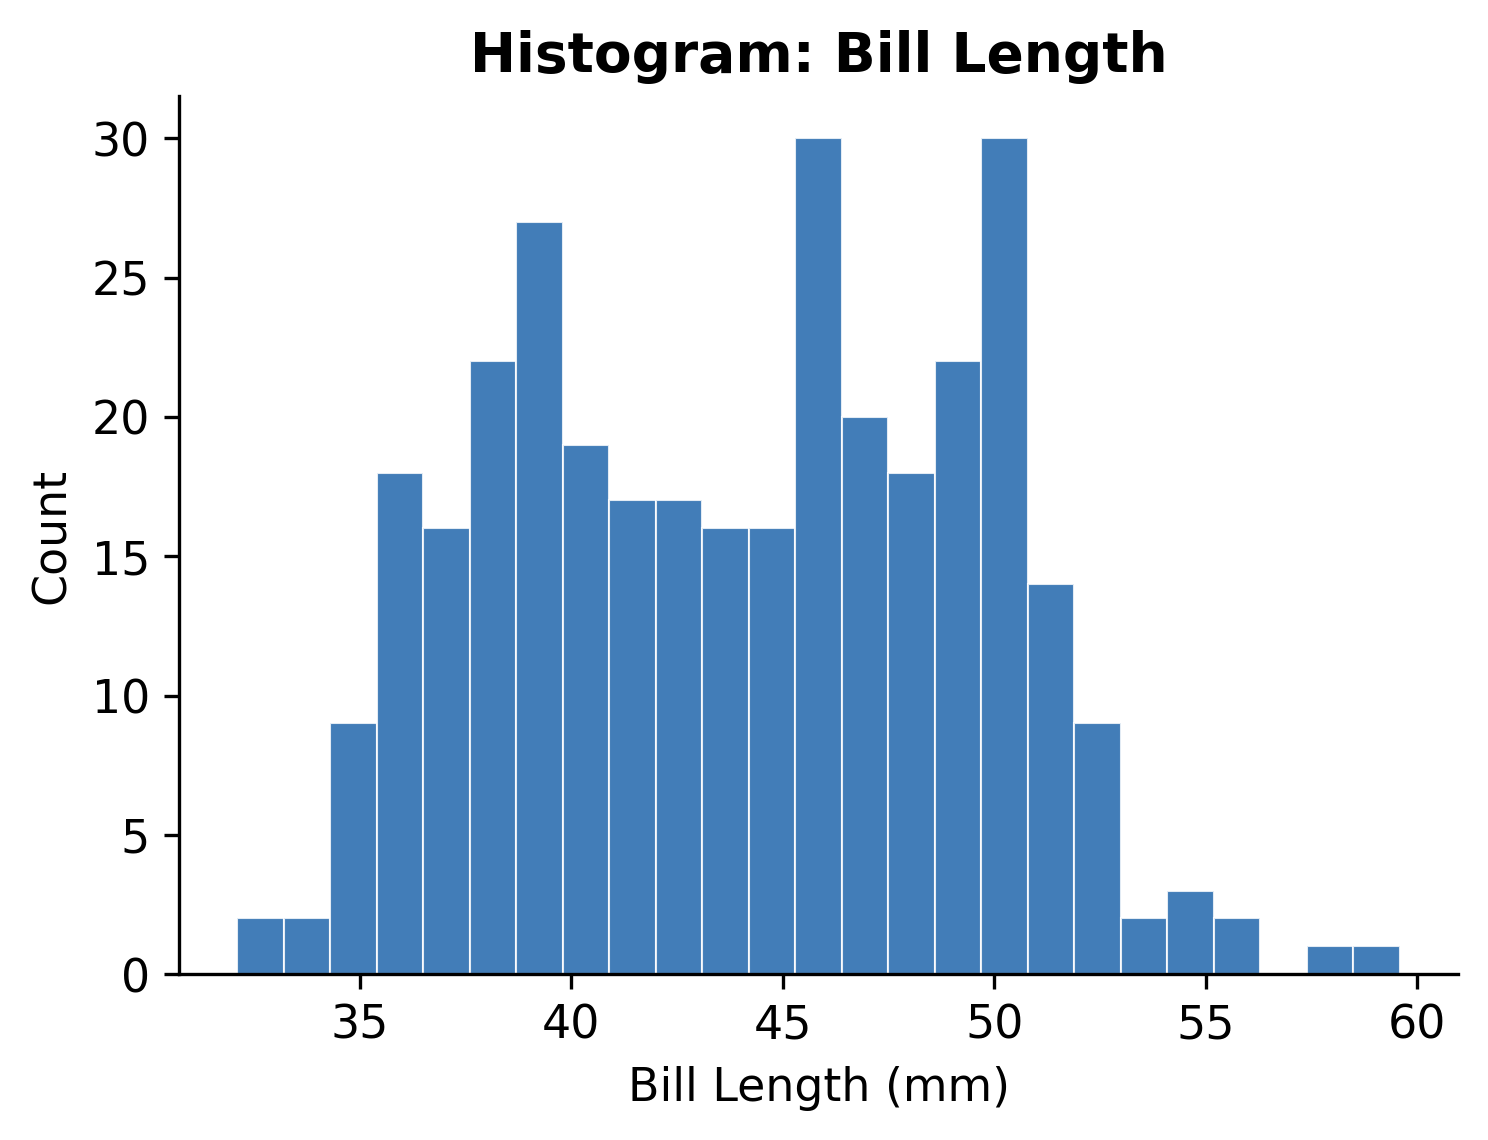
\includegraphics[width=\textwidth]{m1_4_hist_basic.png}
\begin{alertblock}{Pro-Tip}
    \scriptsize Always set \texttt{bins} or \texttt{binwidth} explicitly. The default (30) is arbitrary and rarely optimal.
\end{alertblock}
\end{column}
\end{columns}
\end{frame}

% ── 94 ──
\begin{frame}[fragile]{Basic Histogram --- \Python}\smark{94/300}
\begin{columns}[T]
\begin{column}{0.55\textwidth}
\begin{lstlisting}[style=Pystyle]
# plotnine
(ggplot(penguins,
   aes(x="bill_length_mm"))
 + geom_histogram(bins=25,
     fill="#B2182B", color="white")
 + labs(x="Bill Length (mm)",
        y="Count")
 + theme_minimal())

# matplotlib equivalent
plt.hist(penguins["bill_length_mm"],
         bins=25, color="#B2182B",
         edgecolor="white")
\end{lstlisting}
\end{column}
\begin{column}{0.42\textwidth}
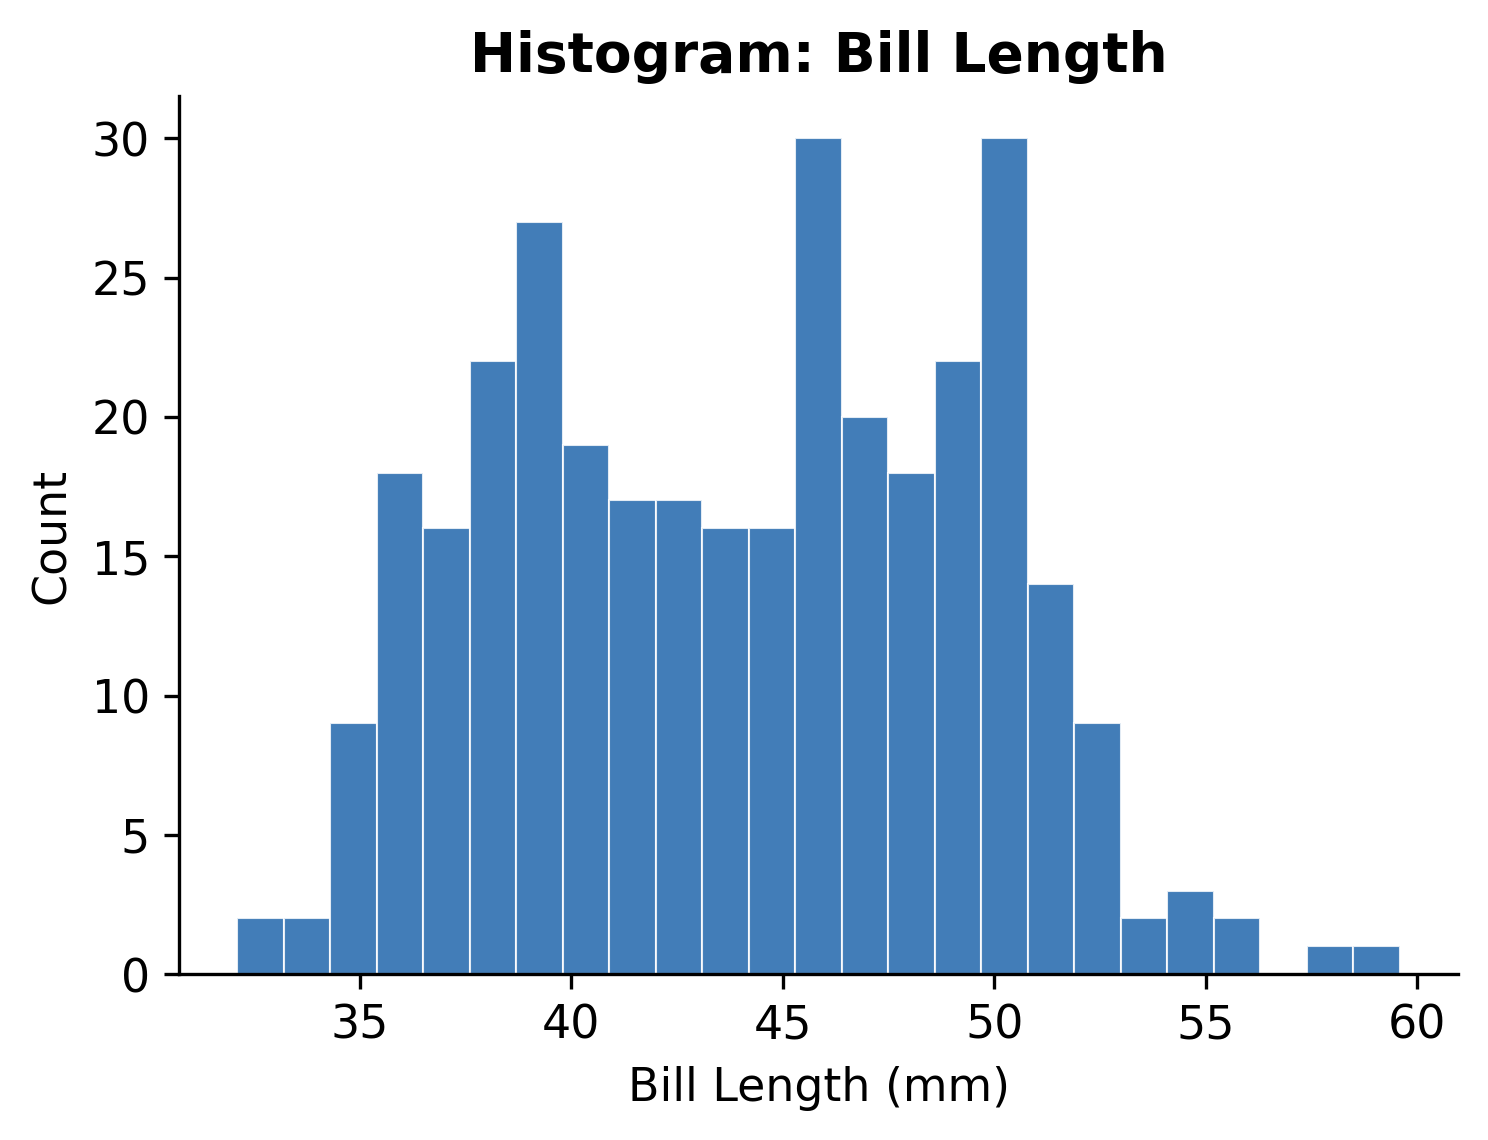
\includegraphics[width=\textwidth]{m1_4_hist_basic.png}
\begin{exampleblock}{Data Insight}
    \scriptsize \texttt{seaborn.histplot()} adds KDE overlay by default with \texttt{kde=True}. Useful for quick exploration.
\end{exampleblock}
\end{column}
\end{columns}
\end{frame}

% ── 95 ──
\begin{frame}{Binwidth Sensitivity}
\smark{95/300}
\centering
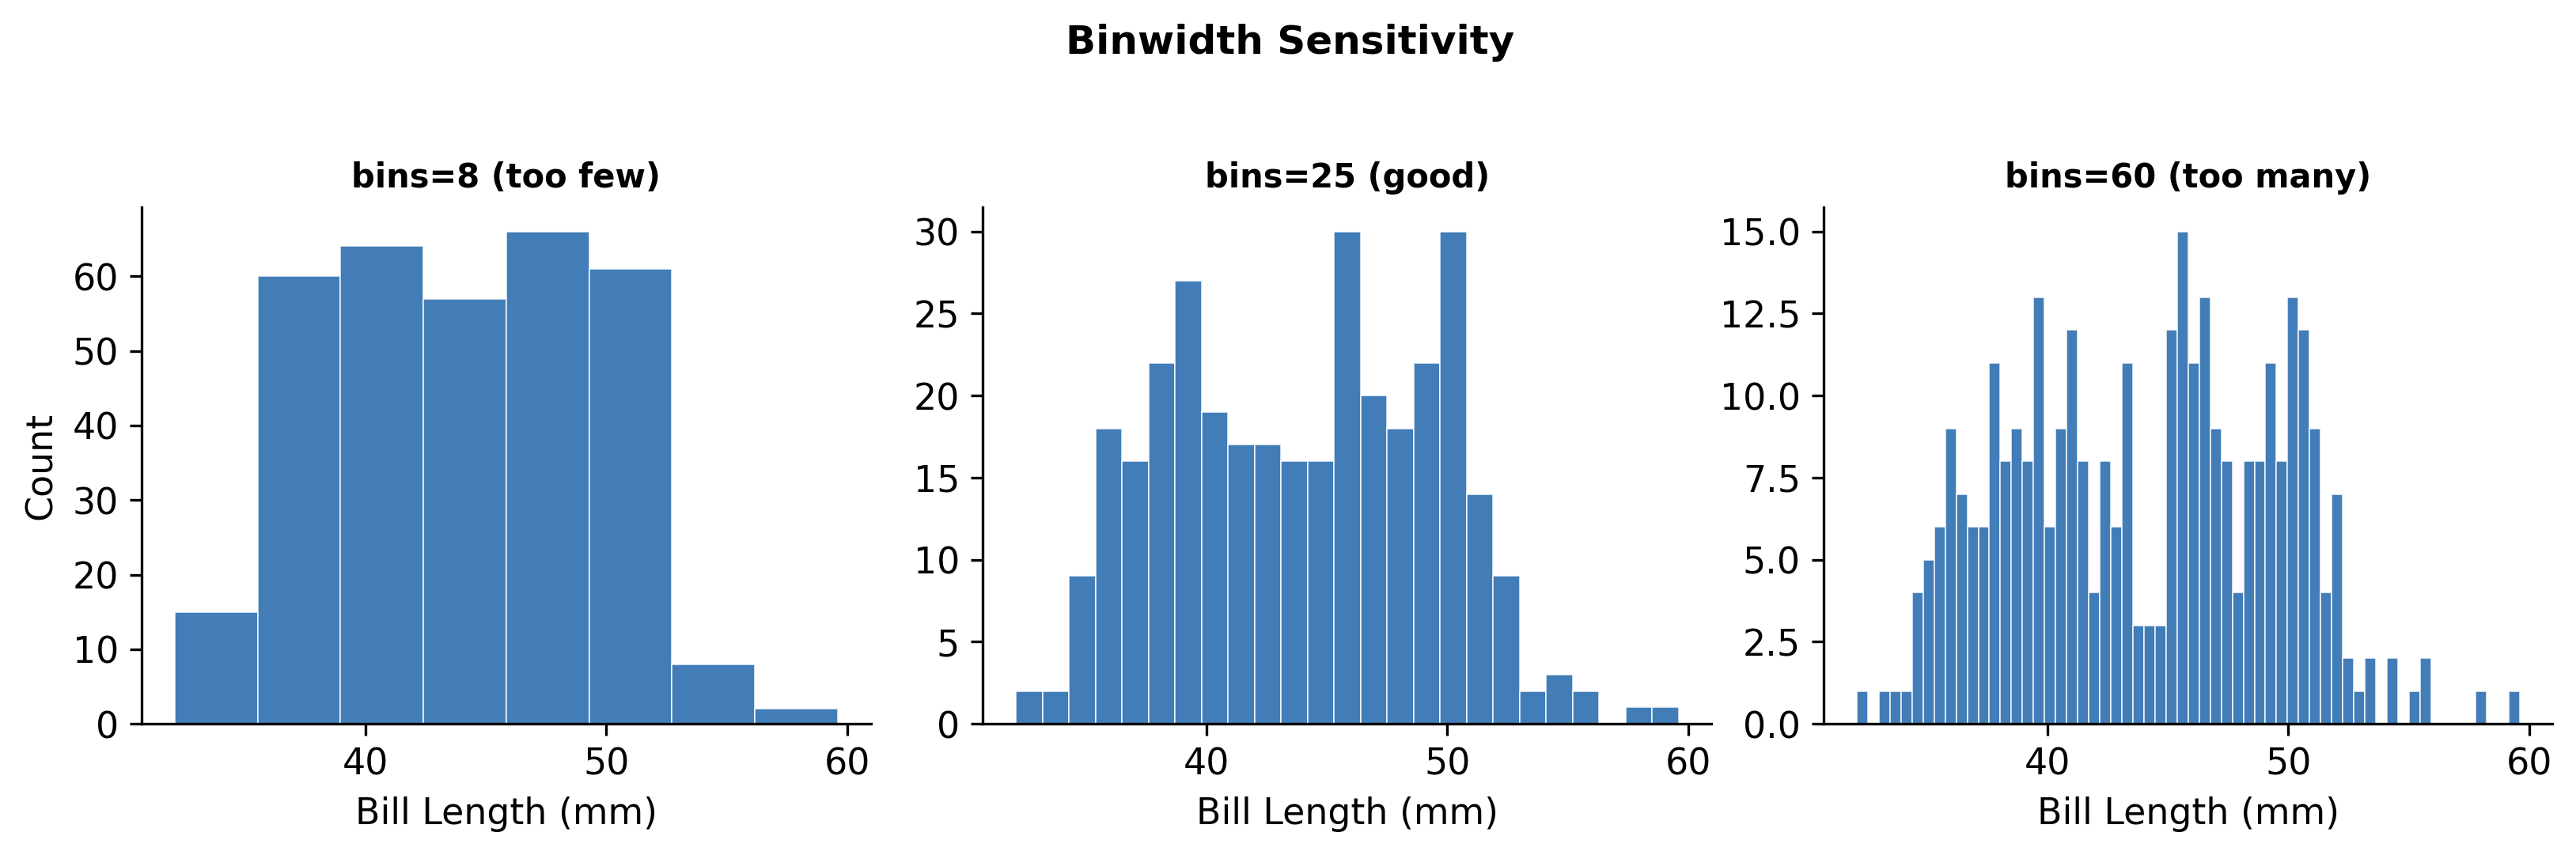
\includegraphics[width=0.92\textwidth]{m1_4_binwidth.png}

\vspace{0.2cm}
\begin{columns}[T]
\begin{column}{0.48\textwidth}
\begin{alertblock}{Pro-Tip}
    \scriptsize Too few bins $\to$ oversmoothed (hides bimodality). Too many $\to$ noisy (spurious peaks). Use Freedman--Diaconis or Sturges' rule as a starting point.
\end{alertblock}
\end{column}
\begin{column}{0.48\textwidth}
\begin{exampleblock}{Data Insight}
    \scriptsize Freedman--Diaconis: $h = 2 \cdot \text{IQR} \cdot n^{-1/3}$. It adapts to data spread and sample size.
\end{exampleblock}
\end{column}
\end{columns}
\end{frame}

% ── 96 ──
\begin{frame}[fragile]{Binwidth Control --- \Rlang}\smark{96/300}
\begin{columns}[T]
\begin{column}{0.55\textwidth}
\begin{lstlisting}[style=Rstyle]
# Fixed number of bins
ggplot(penguins,
  aes(bill_length_mm)) +
  geom_histogram(bins = 15,
    fill="#2166AC", color="white")

# Fixed bin width (mm)
ggplot(penguins,
  aes(bill_length_mm)) +
  geom_histogram(binwidth = 1.5,
    fill="#2166AC", color="white")
\end{lstlisting}
\end{column}
\begin{column}{0.42\textwidth}
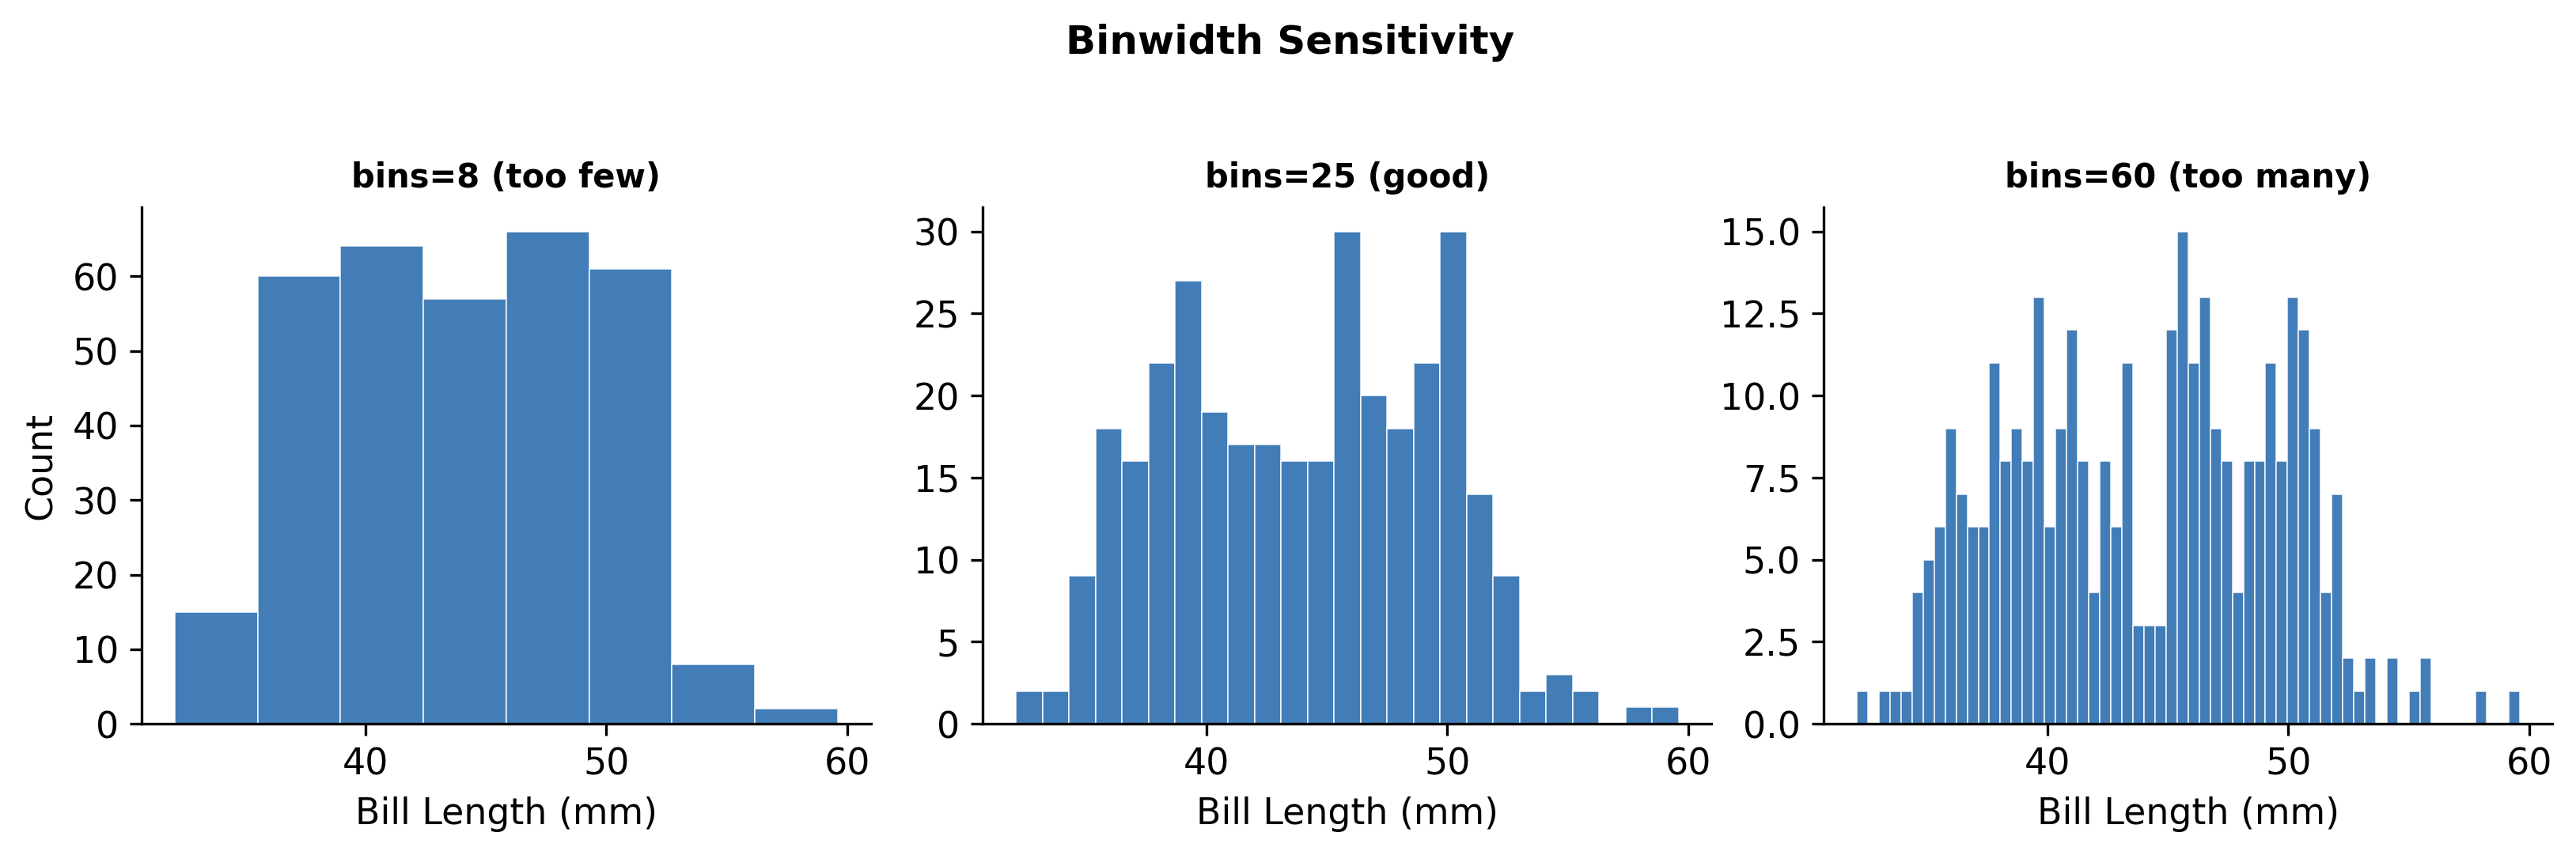
\includegraphics[width=\textwidth]{m1_4_binwidth.png}
\begin{alertblock}{Pro-Tip}
    \scriptsize \texttt{binwidth} is usually more interpretable than \texttt{bins}: ``each bar spans 1.5\,mm'' is a meaningful statement.
\end{alertblock}
\end{column}
\end{columns}
\end{frame}

% ── 97 ──
\begin{frame}[fragile]{Binwidth Control --- \Python}\smark{97/300}
\begin{columns}[T]
\begin{column}{0.55\textwidth}
\begin{lstlisting}[style=Pystyle]
# plotnine: binwidth parameter
(ggplot(penguins,
   aes("bill_length_mm"))
 + geom_histogram(binwidth=1.5,
     fill="#B2182B", color="white"))

# matplotlib: bins or range
plt.hist(penguins["bill_length_mm"],
  bins=np.arange(30, 62, 1.5),
  color="#B2182B", edgecolor="white")
\end{lstlisting}
\end{column}
\begin{column}{0.42\textwidth}
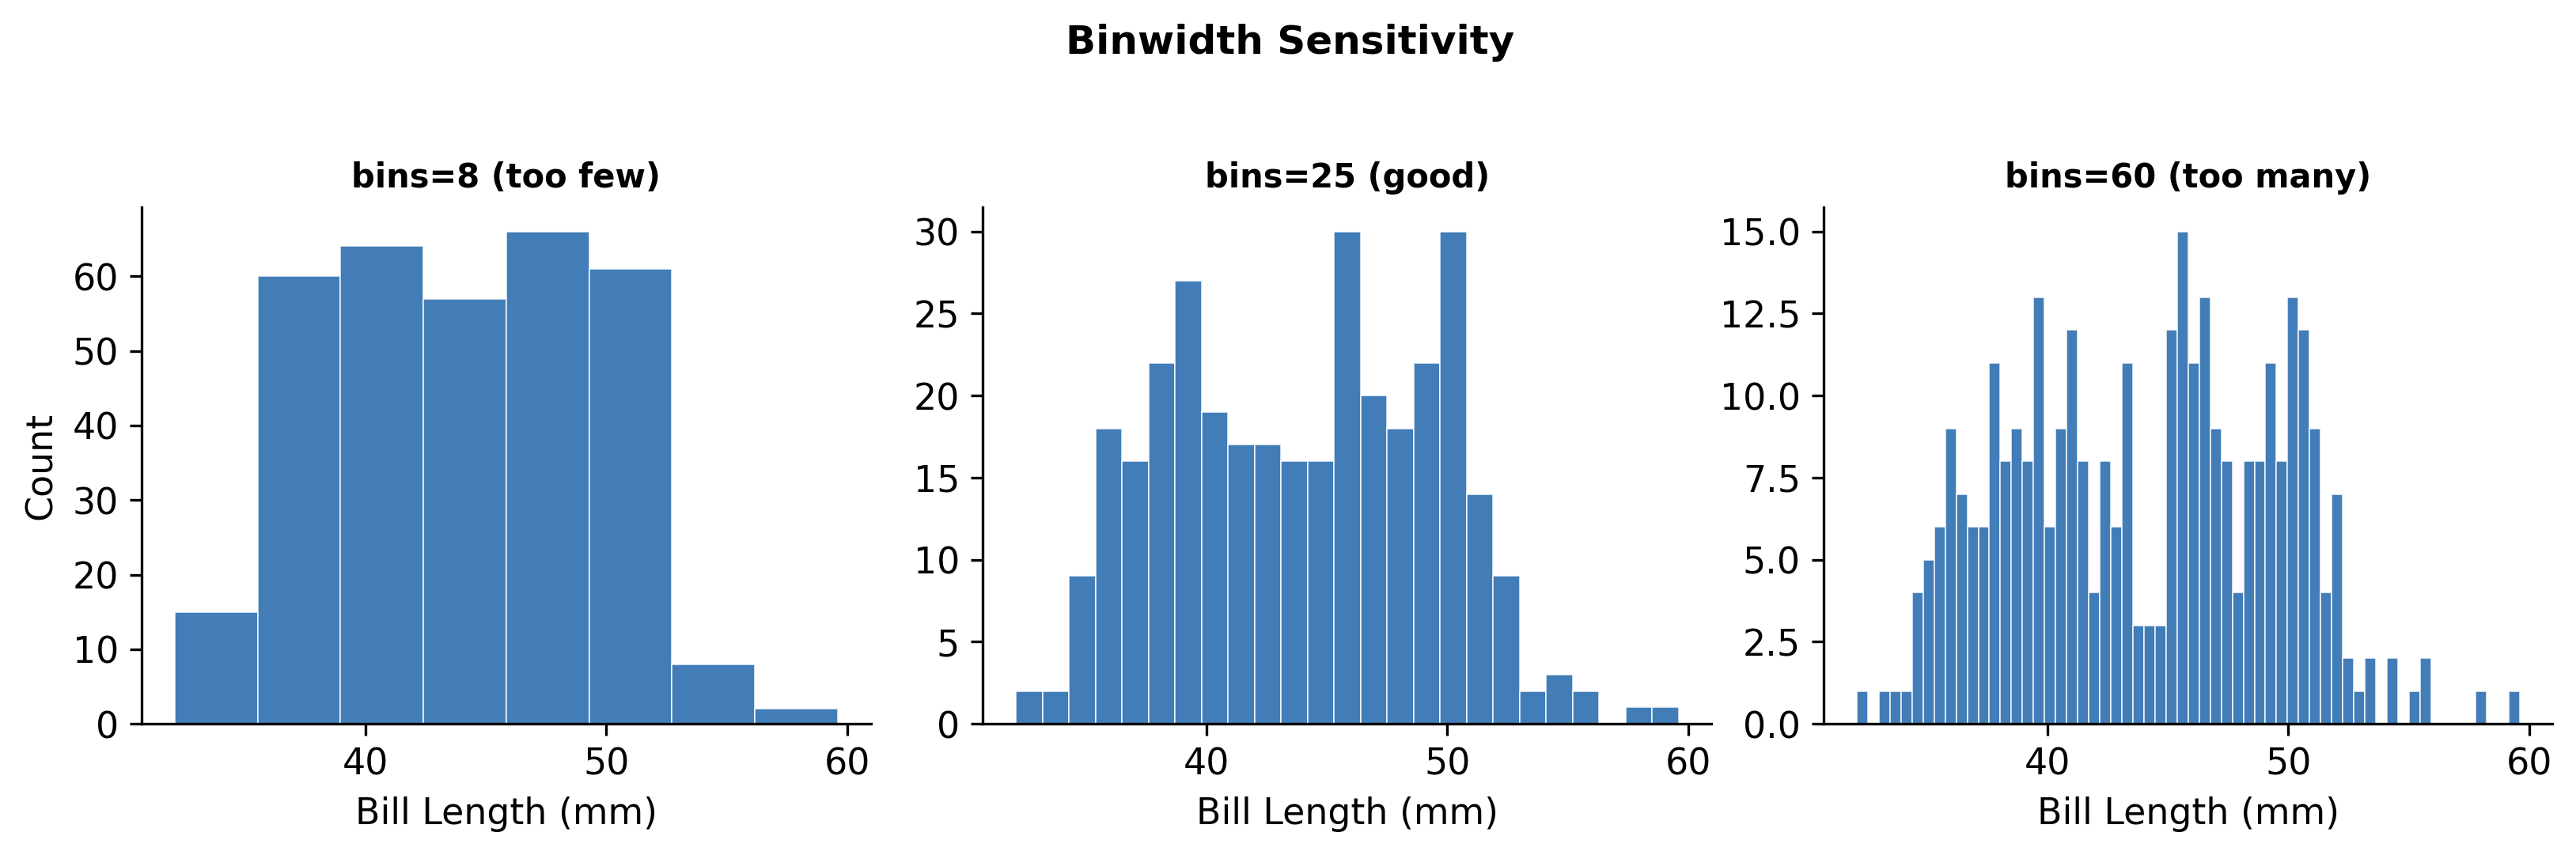
\includegraphics[width=\textwidth]{m1_4_binwidth.png}
\begin{exampleblock}{Data Insight}
    \scriptsize In matplotlib, pass an array to \texttt{bins} for exact control: \texttt{np.arange(start, stop, width)}.
\end{exampleblock}
\end{column}
\end{columns}
\end{frame}

% ── 98 ──
\begin{frame}{Frequency Polygons}
\smark{98/300}
\begin{columns}[T]
\begin{column}{0.50\textwidth}
\begin{itemize}
    \item Connect bin midpoints with a line
    \item Same information as histogram, less ink
    \item Easier to \textbf{overlay multiple groups} (no occlusion)
    \item In ggplot2: \texttt{geom\_freqpoly()}
\end{itemize}
\end{column}
\begin{column}{0.47\textwidth}
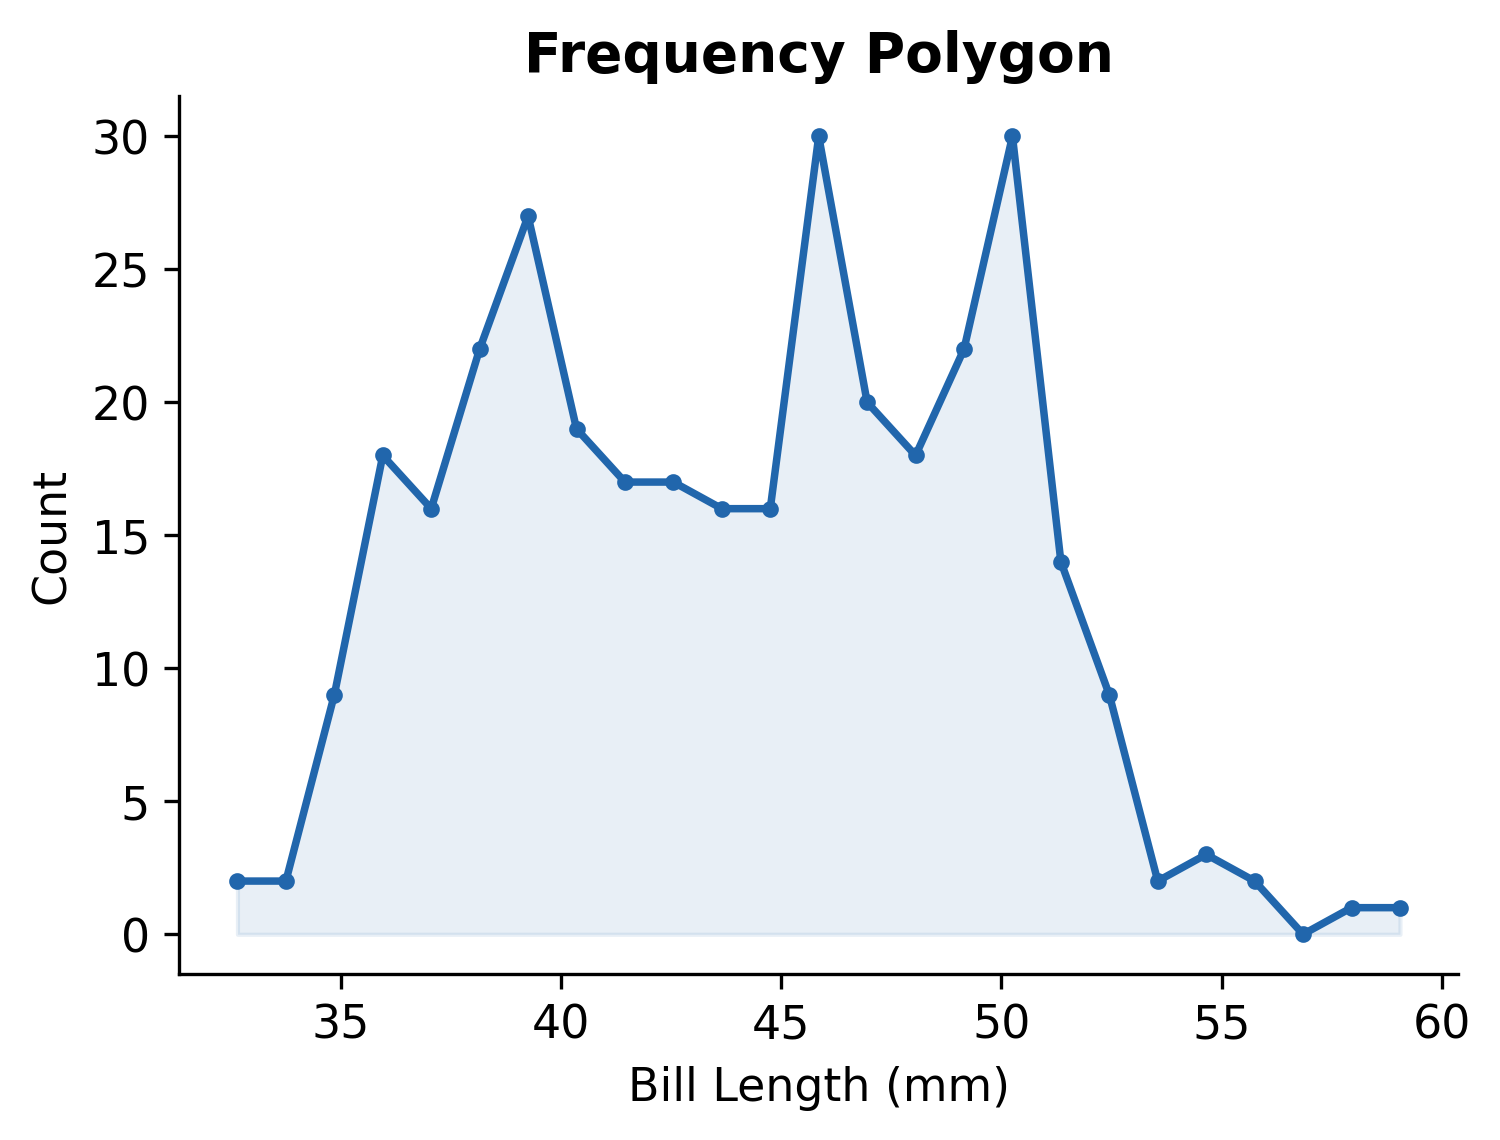
\includegraphics[width=\textwidth]{m1_4_freqpoly.png}
\begin{exampleblock}{Data Insight}
    \scriptsize Frequency polygons excel when comparing 3+ distributions on the same axes --- overlapping histograms become unreadable.
\end{exampleblock}
\end{column}
\end{columns}
\end{frame}

% ── 99 ──
\begin{frame}[fragile]{Frequency Polygon --- \Rlang}\smark{99/300}
\begin{columns}[T]
\begin{column}{0.55\textwidth}
\begin{lstlisting}[style=Rstyle]
# Single distribution
ggplot(penguins,
  aes(bill_length_mm)) +
  geom_freqpoly(bins = 25,
    color = "#2166AC",
    linewidth = 1) +
  theme_minimal()

# Grouped by species
ggplot(penguins,
  aes(bill_length_mm,
      color = species)) +
  geom_freqpoly(bins = 20,
    linewidth = 0.8) +
  scale_color_manual(
    values = c("#1B9E77","#D95F02",
               "#7570B3"))
\end{lstlisting}
\end{column}
\begin{column}{0.42\textwidth}
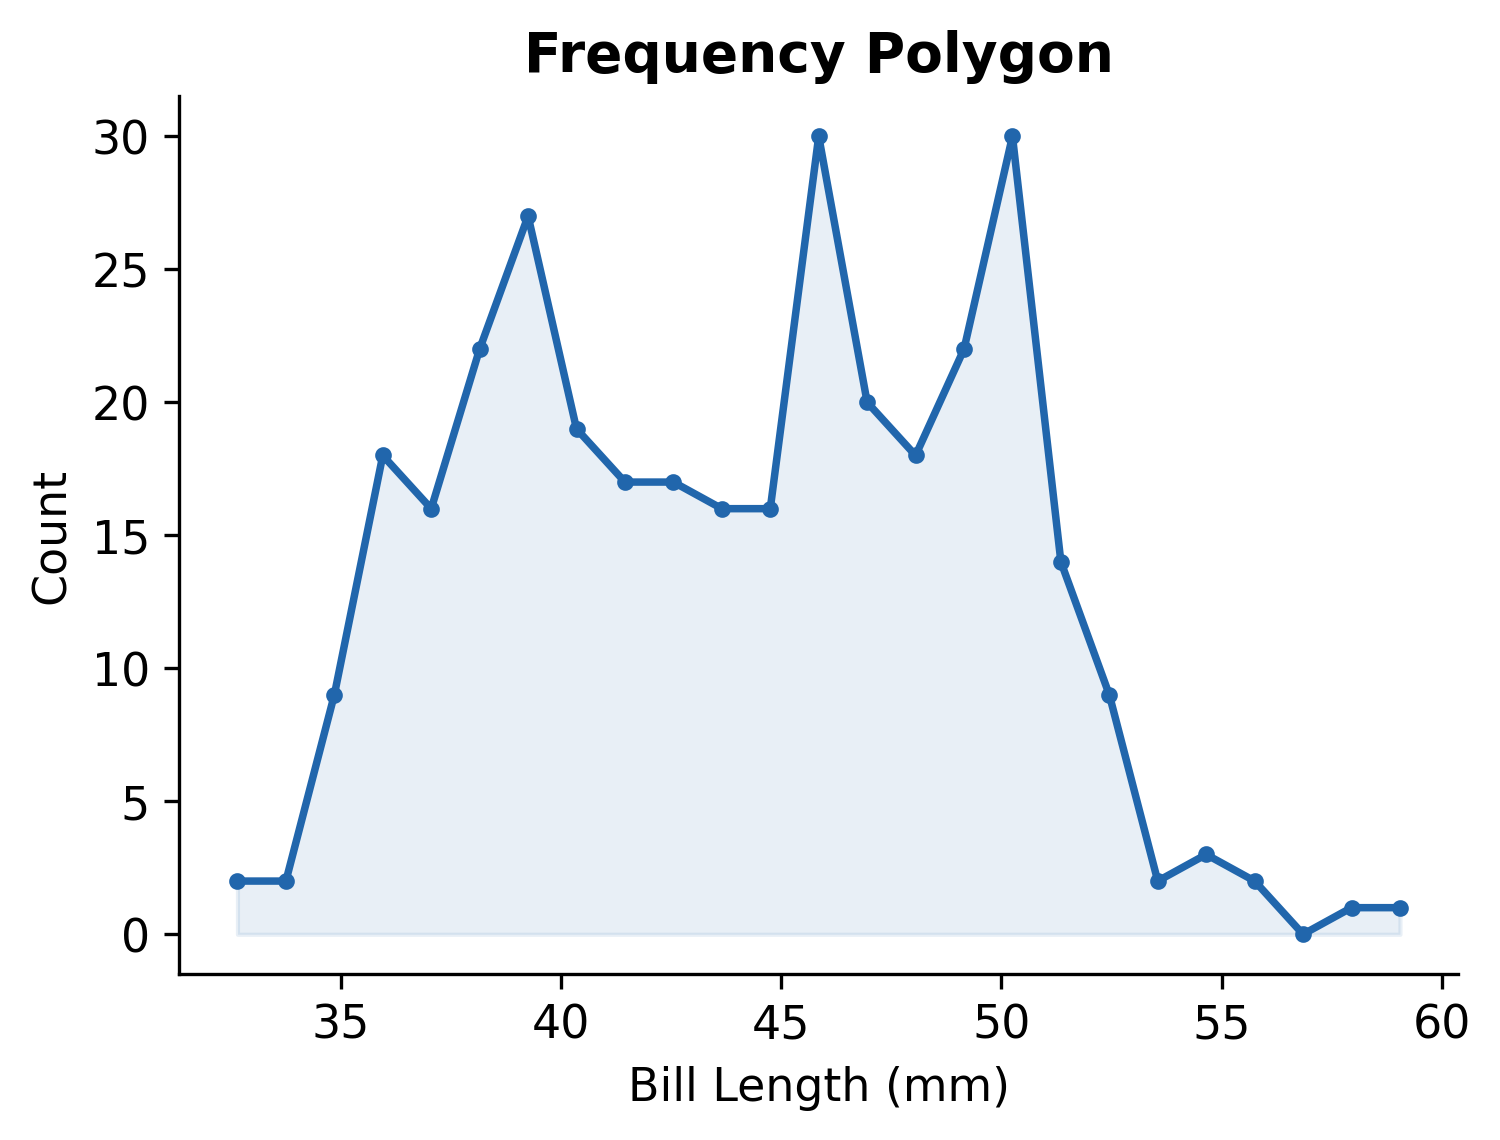
\includegraphics[width=\textwidth]{m1_4_freqpoly.png}
\begin{alertblock}{Pro-Tip}
    \scriptsize \texttt{geom\_freqpoly()} shares the same \texttt{bins}/\texttt{binwidth} parameters as \texttt{geom\_histogram()}.
\end{alertblock}
\end{column}
\end{columns}
\end{frame}

% ── 100 ──
\begin{frame}[fragile]{Frequency Polygon --- \Python}\smark{100/300}
\begin{columns}[T]
\begin{column}{0.55\textwidth}
\begin{lstlisting}[style=Pystyle]
# plotnine
(ggplot(penguins,
   aes("bill_length_mm",
       color="species"))
 + geom_freqpoly(bins=20, size=1)
 + theme_minimal())

# matplotlib (manual)
counts, edges = np.histogram(
    data, bins=25)
centers = (edges[:-1]+edges[1:])/2
plt.plot(centers, counts,
         color="#B2182B")
\end{lstlisting}
\end{column}
\begin{column}{0.42\textwidth}
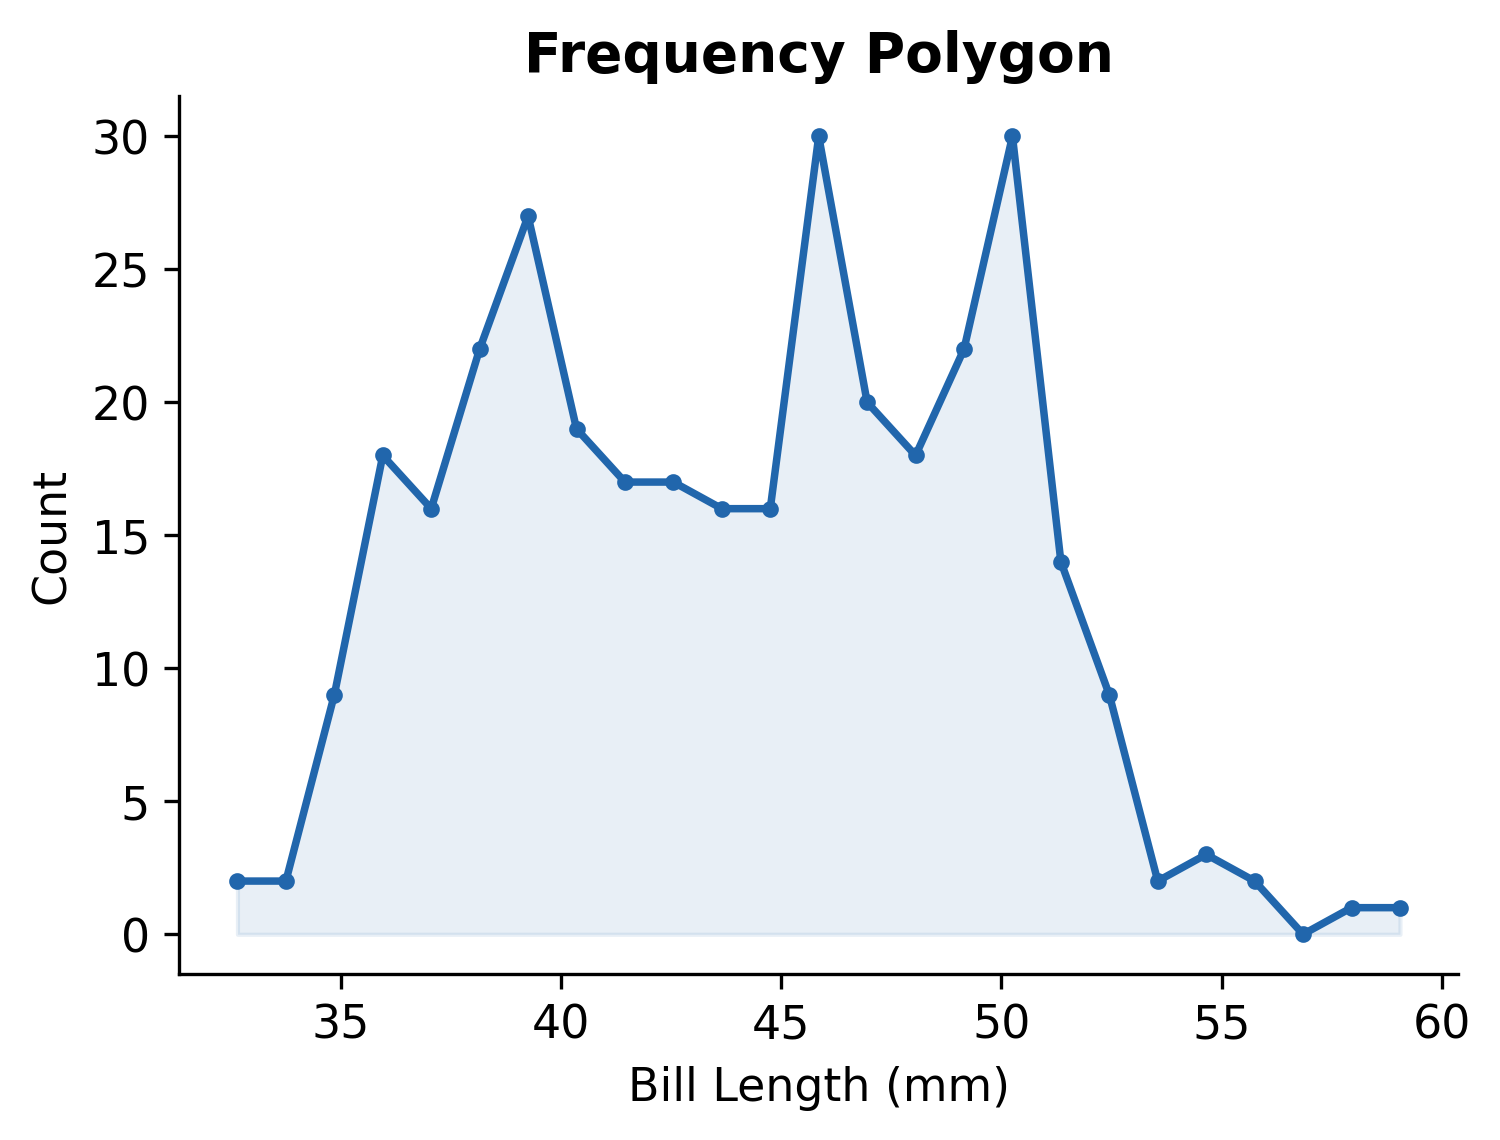
\includegraphics[width=\textwidth]{m1_4_freqpoly.png}
\begin{exampleblock}{Data Insight}
    \scriptsize matplotlib has no built-in frequency polygon. Compute \texttt{np.histogram()}, take bin centers, and \texttt{plt.plot()}.
\end{exampleblock}
\end{column}
\end{columns}
\end{frame}

% ── 101 ──
\begin{frame}{Kernel Density Estimation (KDE): Theory}
\smark{101/300}
\begin{columns}[T]
\begin{column}{0.52\textwidth}
\begin{itemize}
    \item Place a \textbf{kernel} (e.g., Gaussian) at each data point
    \item Sum all kernels $\to$ smooth density curve
    \item \textbf{Bandwidth} ($h$) controls smoothing: small $h$ = wiggly, large $h$ = flat
    \item No binning artifacts --- continuous estimate
\end{itemize}
\vspace{0.1cm}
$\hat{f}(x) = \frac{1}{nh}\sum_{i=1}^{n} K\!\left(\frac{x - x_i}{h}\right)$
\end{column}
\begin{column}{0.45\textwidth}
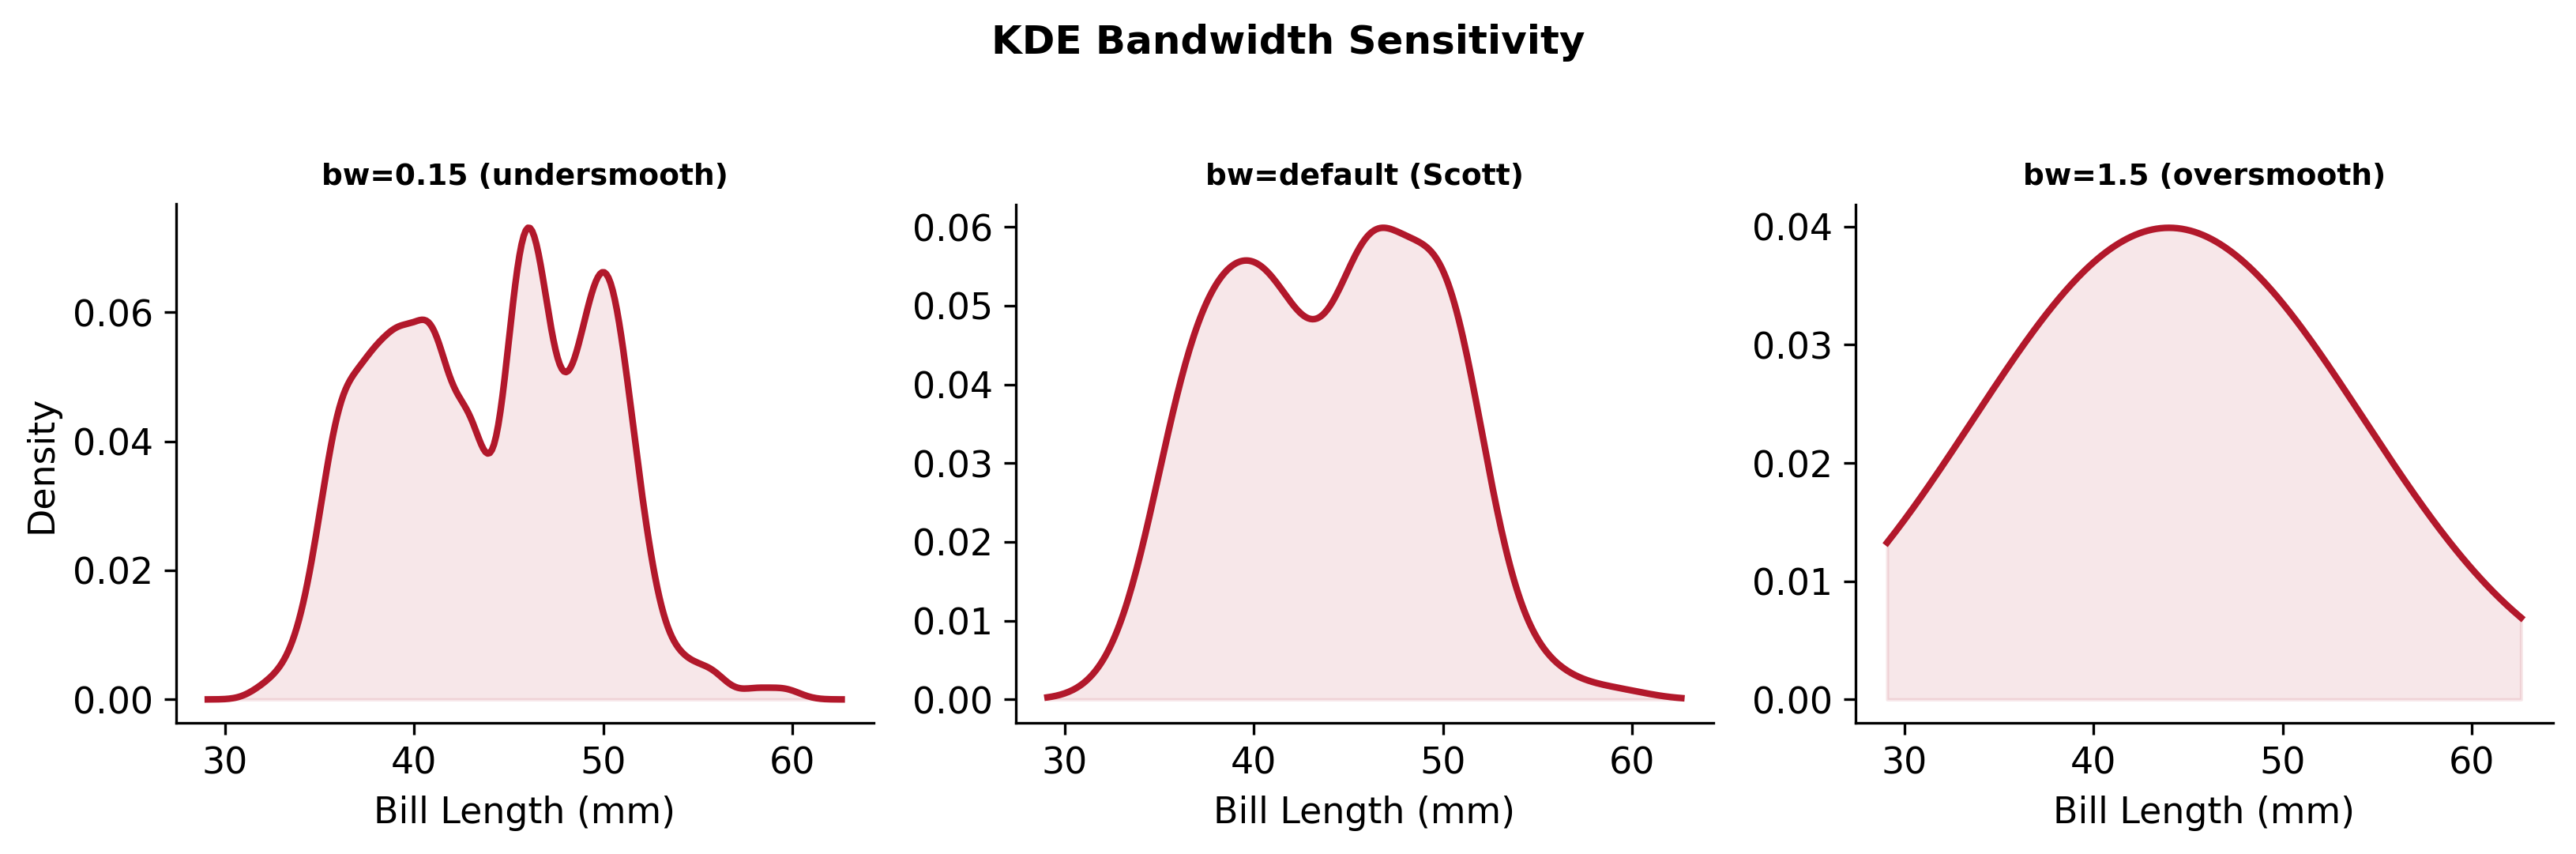
\includegraphics[width=\textwidth]{m1_4_bandwidth.png}
\begin{alertblock}{Pro-Tip}
    \scriptsize Scott's rule ($h = 1.06\,s\,n^{-1/5}$) is the default in most software. Override only with reason.
\end{alertblock}
\end{column}
\end{columns}
\end{frame}

% ── 102 ──
\begin{frame}[fragile]{KDE --- \Rlang}\smark{102/300}
\begin{columns}[T]
\begin{column}{0.55\textwidth}
\begin{lstlisting}[style=Rstyle]
# Default KDE
ggplot(penguins,
  aes(bill_length_mm)) +
  geom_density(fill = "#2166AC",
    alpha = 0.3, color="#2166AC",
    linewidth = 1) +
  theme_minimal()

# Adjust bandwidth
ggplot(penguins,
  aes(bill_length_mm)) +
  geom_density(adjust = 0.5,
    fill = "#2166AC", alpha=0.3)
# adjust < 1 = less smooth
# adjust > 1 = more smooth
\end{lstlisting}
\end{column}
\begin{column}{0.42\textwidth}
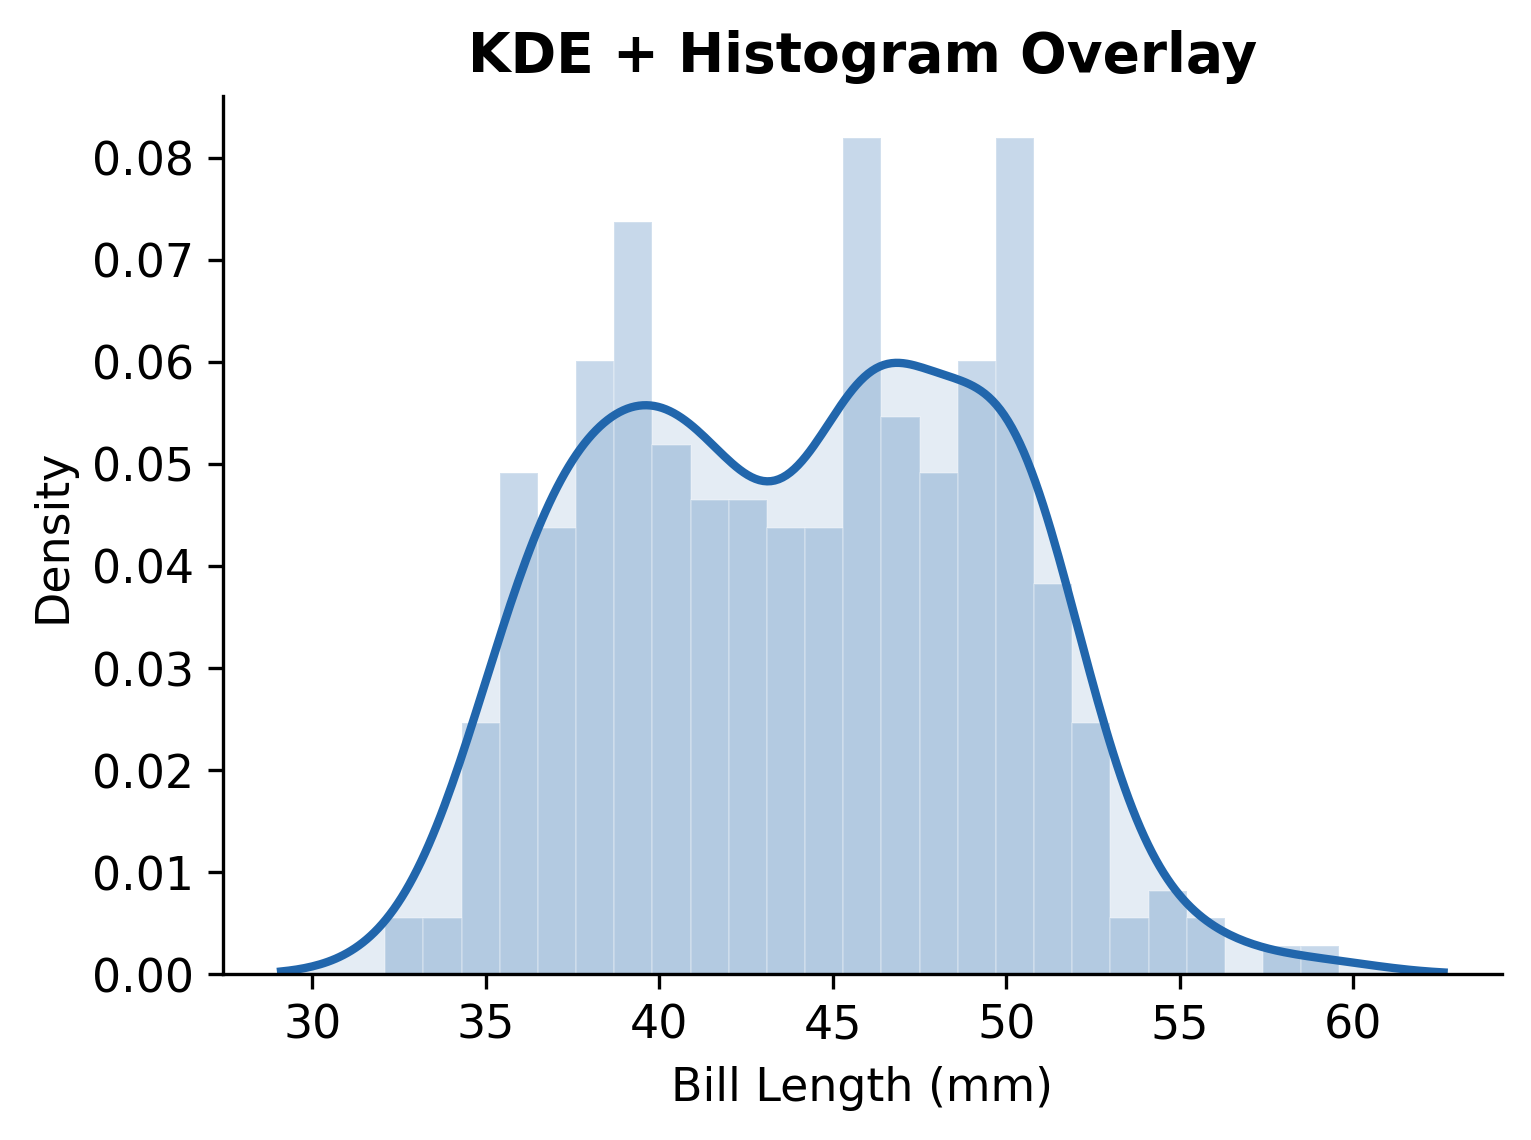
\includegraphics[width=\textwidth]{m1_4_kde_basic.png}
\begin{exampleblock}{Data Insight}
    \scriptsize \texttt{adjust} is a multiplier on the default bandwidth: \texttt{adjust=0.5} halves $h$, revealing finer structure.
\end{exampleblock}
\end{column}
\end{columns}
\end{frame}

% ── 103 ──
\begin{frame}[fragile]{KDE --- \Python}\smark{103/300}
\begin{columns}[T]
\begin{column}{0.55\textwidth}
\begin{lstlisting}[style=Pystyle]
# plotnine
(ggplot(penguins,
   aes("bill_length_mm"))
 + geom_density(fill="#B2182B",
     alpha=0.3, color="#B2182B"))

# seaborn
sns.kdeplot(penguins["bill_length_mm"],
    fill=True, color="#B2182B",
    bw_adjust=0.5)

# scipy (manual)
from scipy.stats import gaussian_kde
kde = gaussian_kde(data, bw_method=0.3)
plt.plot(xs, kde(xs))
\end{lstlisting}
\end{column}
\begin{column}{0.42\textwidth}
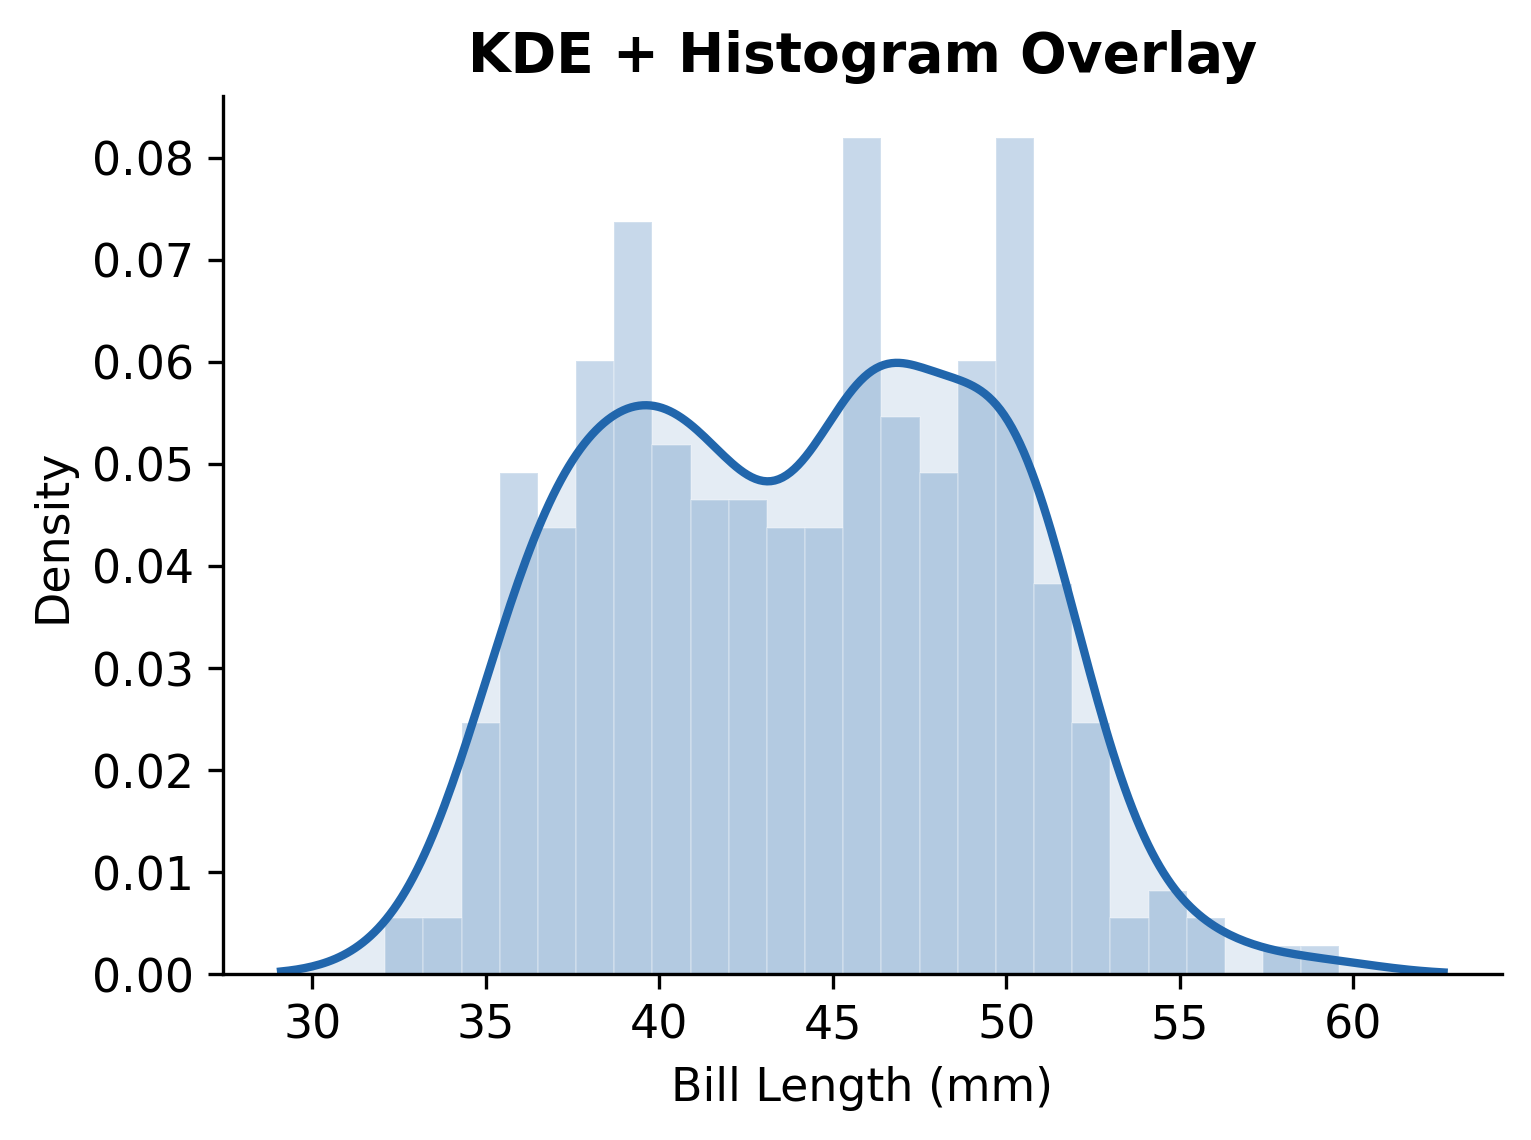
\includegraphics[width=\textwidth]{m1_4_kde_basic.png}
\begin{alertblock}{Pro-Tip}
    \scriptsize \texttt{seaborn.kdeplot(bw\_adjust=)} mirrors ggplot2's \texttt{adjust}. \texttt{scipy} uses \texttt{bw\_method} as an absolute or callable.
\end{alertblock}
\end{column}
\end{columns}
\end{frame}

% ── 104 ──
\begin{frame}{Histogram + Density + Rug: The Triple Layer}
\smark{104/300}
\centering
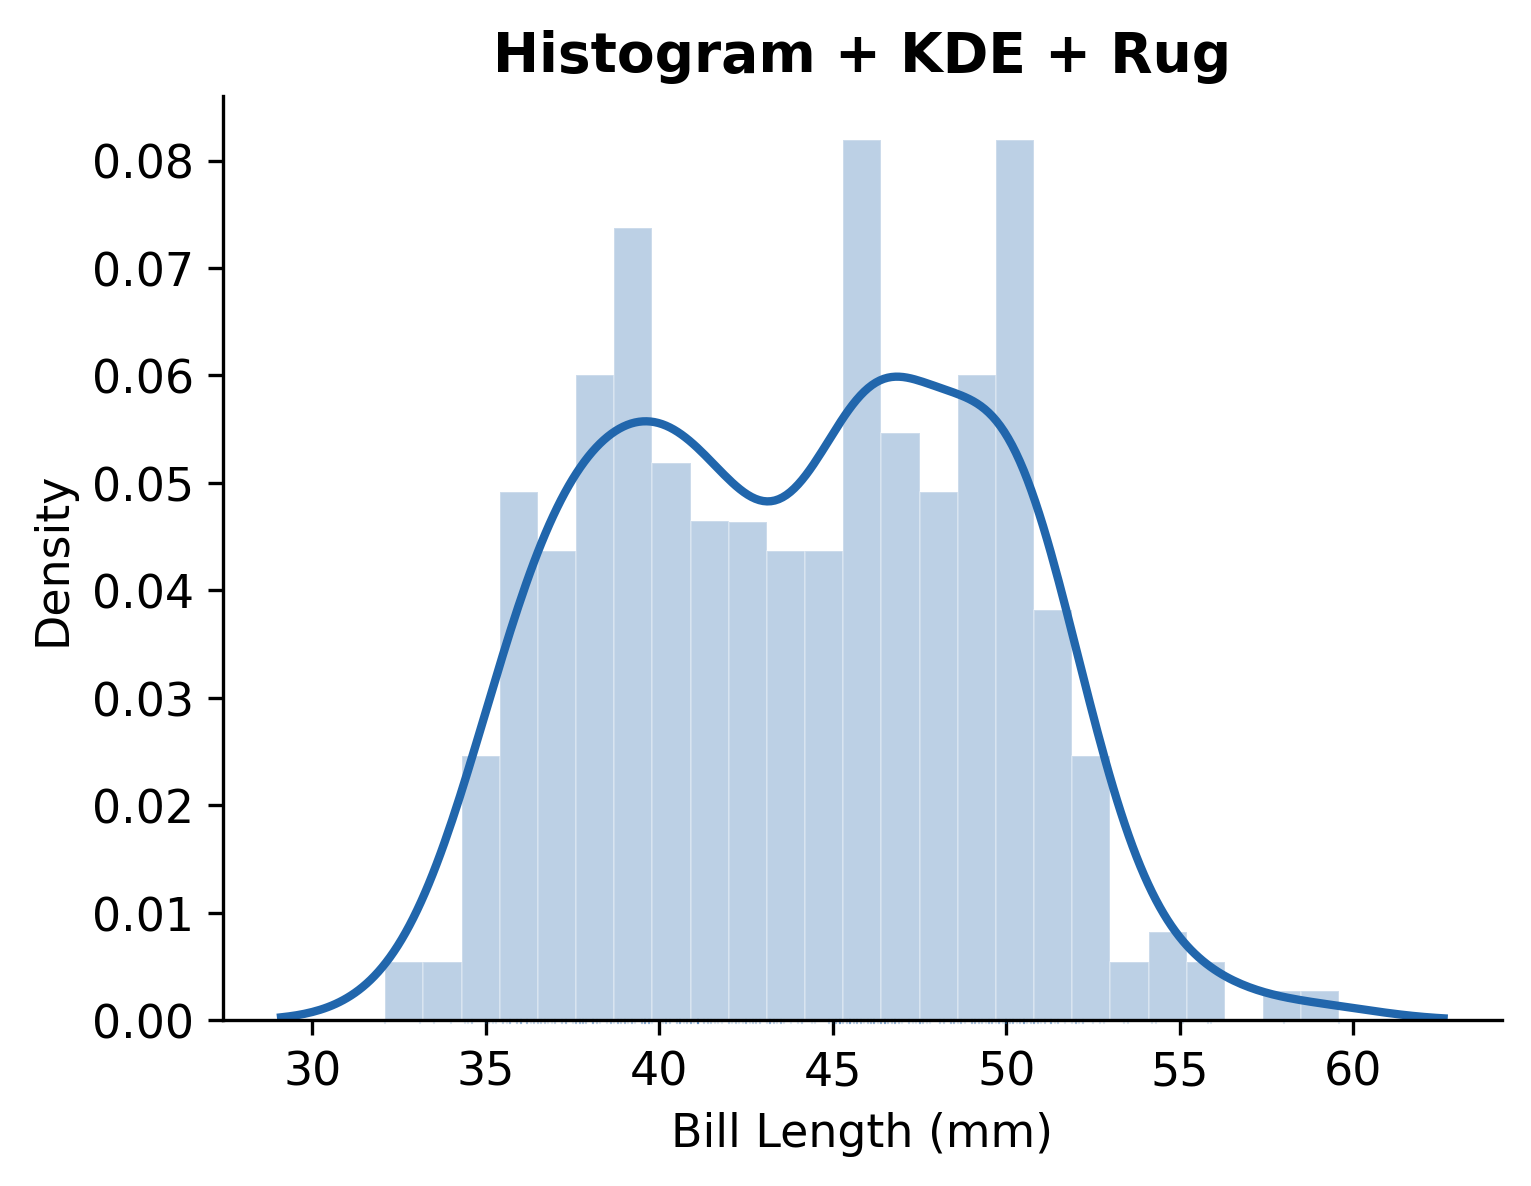
\includegraphics[width=0.7\textwidth]{m1_4_hist_kde_rug.png}

\vspace{0.2cm}
\begin{columns}[T]
\begin{column}{0.48\textwidth}
\begin{exampleblock}{Data Insight}
    \scriptsize The histogram shows \emph{binned counts}, the KDE shows \emph{smooth shape}, and the rug shows \emph{every individual observation}. Three complementary views.
\end{exampleblock}
\end{column}
\begin{column}{0.48\textwidth}
\begin{alertblock}{Pro-Tip}
    \scriptsize To overlay histogram + density, set the histogram to \texttt{y = after\_stat(density)} in R or \texttt{stat="density"} in plotnine so both share the $y$-axis.
\end{alertblock}
\end{column}
\end{columns}
\end{frame}

% ── 105 ──
\begin{frame}[fragile]{Triple Layer --- \Rlang}\smark{105/300}
\begin{columns}[T]
\begin{column}{0.55\textwidth}
\begin{lstlisting}[style=Rstyle]
ggplot(penguins,
  aes(bill_length_mm)) +
  geom_histogram(
    aes(y = after_stat(density)),
    bins = 25, fill = "#2166AC",
    alpha = 0.3, color="white") +
  geom_density(color = "#2166AC",
    linewidth = 1) +
  geom_rug(alpha = 0.15) +
  theme_minimal()
\end{lstlisting}
\end{column}
\begin{column}{0.42\textwidth}
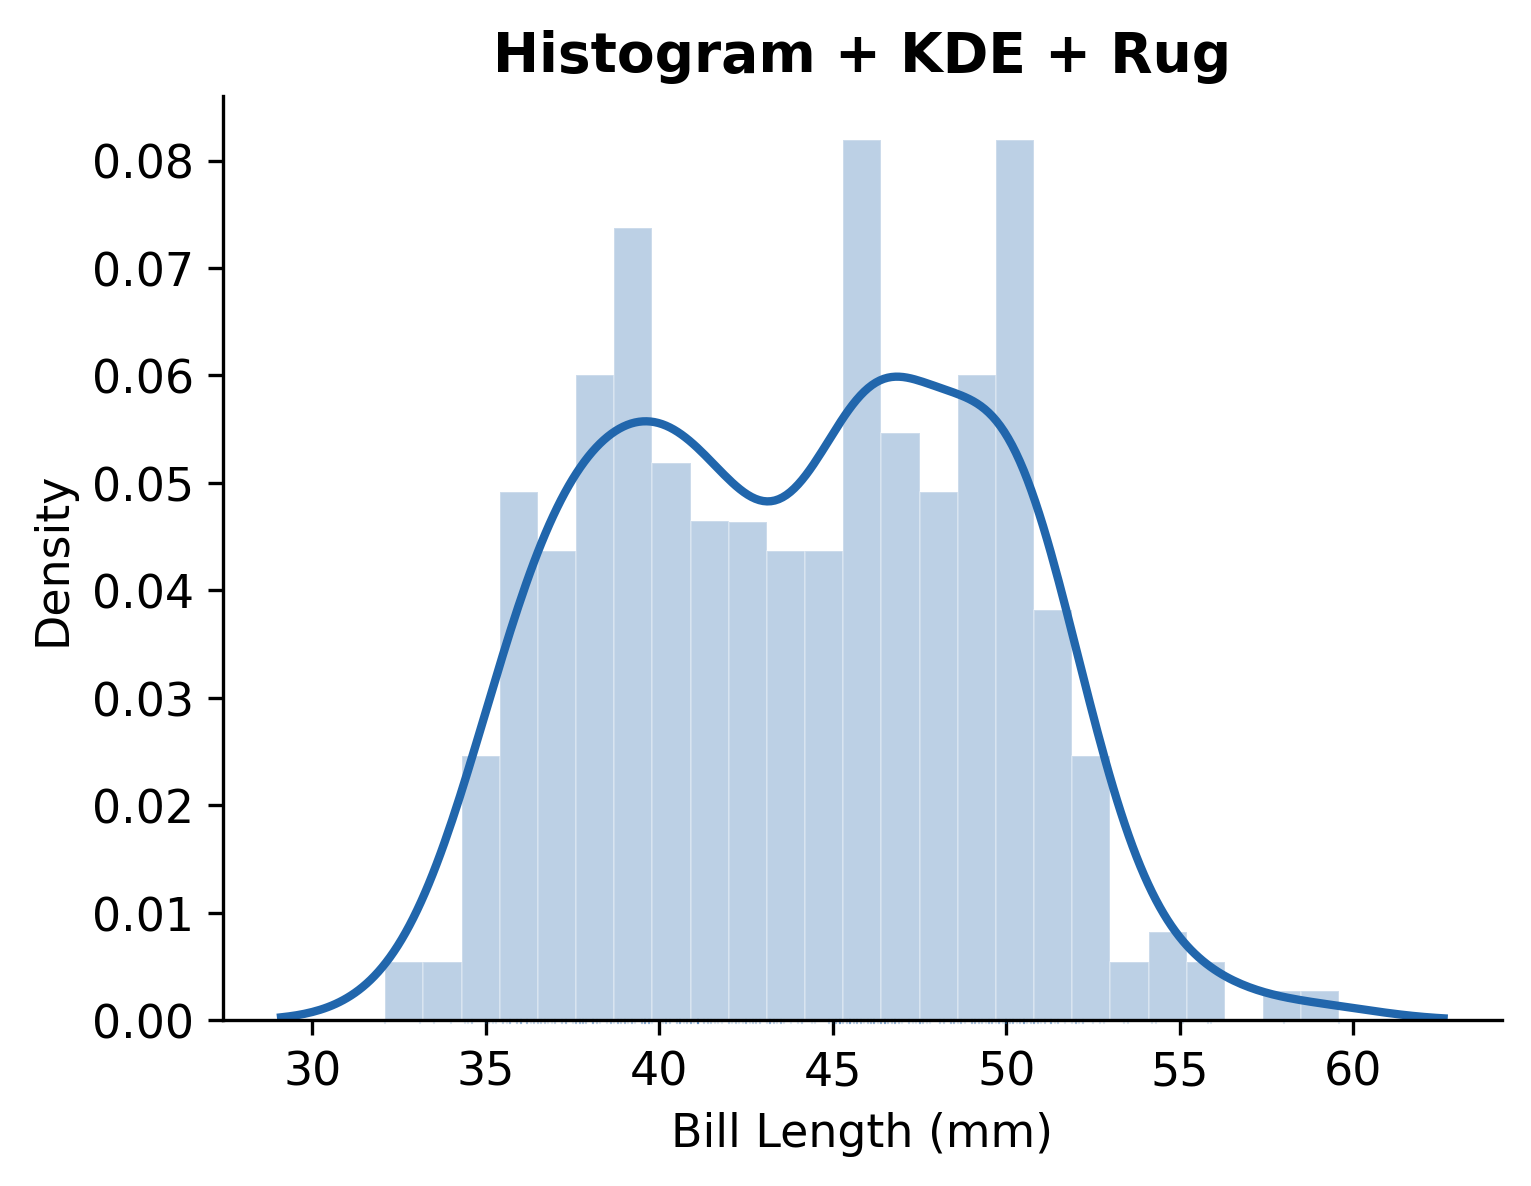
\includegraphics[width=\textwidth]{m1_4_hist_kde_rug.png}
\begin{alertblock}{Pro-Tip}
    \scriptsize \texttt{after\_stat(density)} rescales histogram bars to density (area = 1), matching the KDE's $y$-axis.
\end{alertblock}
\end{column}
\end{columns}
\end{frame}

% ── 106 ──
\begin{frame}[fragile]{Triple Layer --- \Python}\smark{106/300}
\begin{columns}[T]
\begin{column}{0.55\textwidth}
\begin{lstlisting}[style=Pystyle]
# plotnine
(ggplot(penguins,
   aes("bill_length_mm"))
 + geom_histogram(
     aes(y="after_stat('density')"),
     bins=25, fill="#B2182B",
     alpha=0.3, color="white")
 + geom_density(color="#B2182B")
 + geom_rug(alpha=0.15))

# seaborn (one-liner)
sns.histplot(
    penguins["bill_length_mm"],
    kde=True, stat="density",
    color="#B2182B", alpha=0.3)
plt.rug(penguins["bill_length_mm"],
        alpha=0.1)
\end{lstlisting}
\end{column}
\begin{column}{0.42\textwidth}
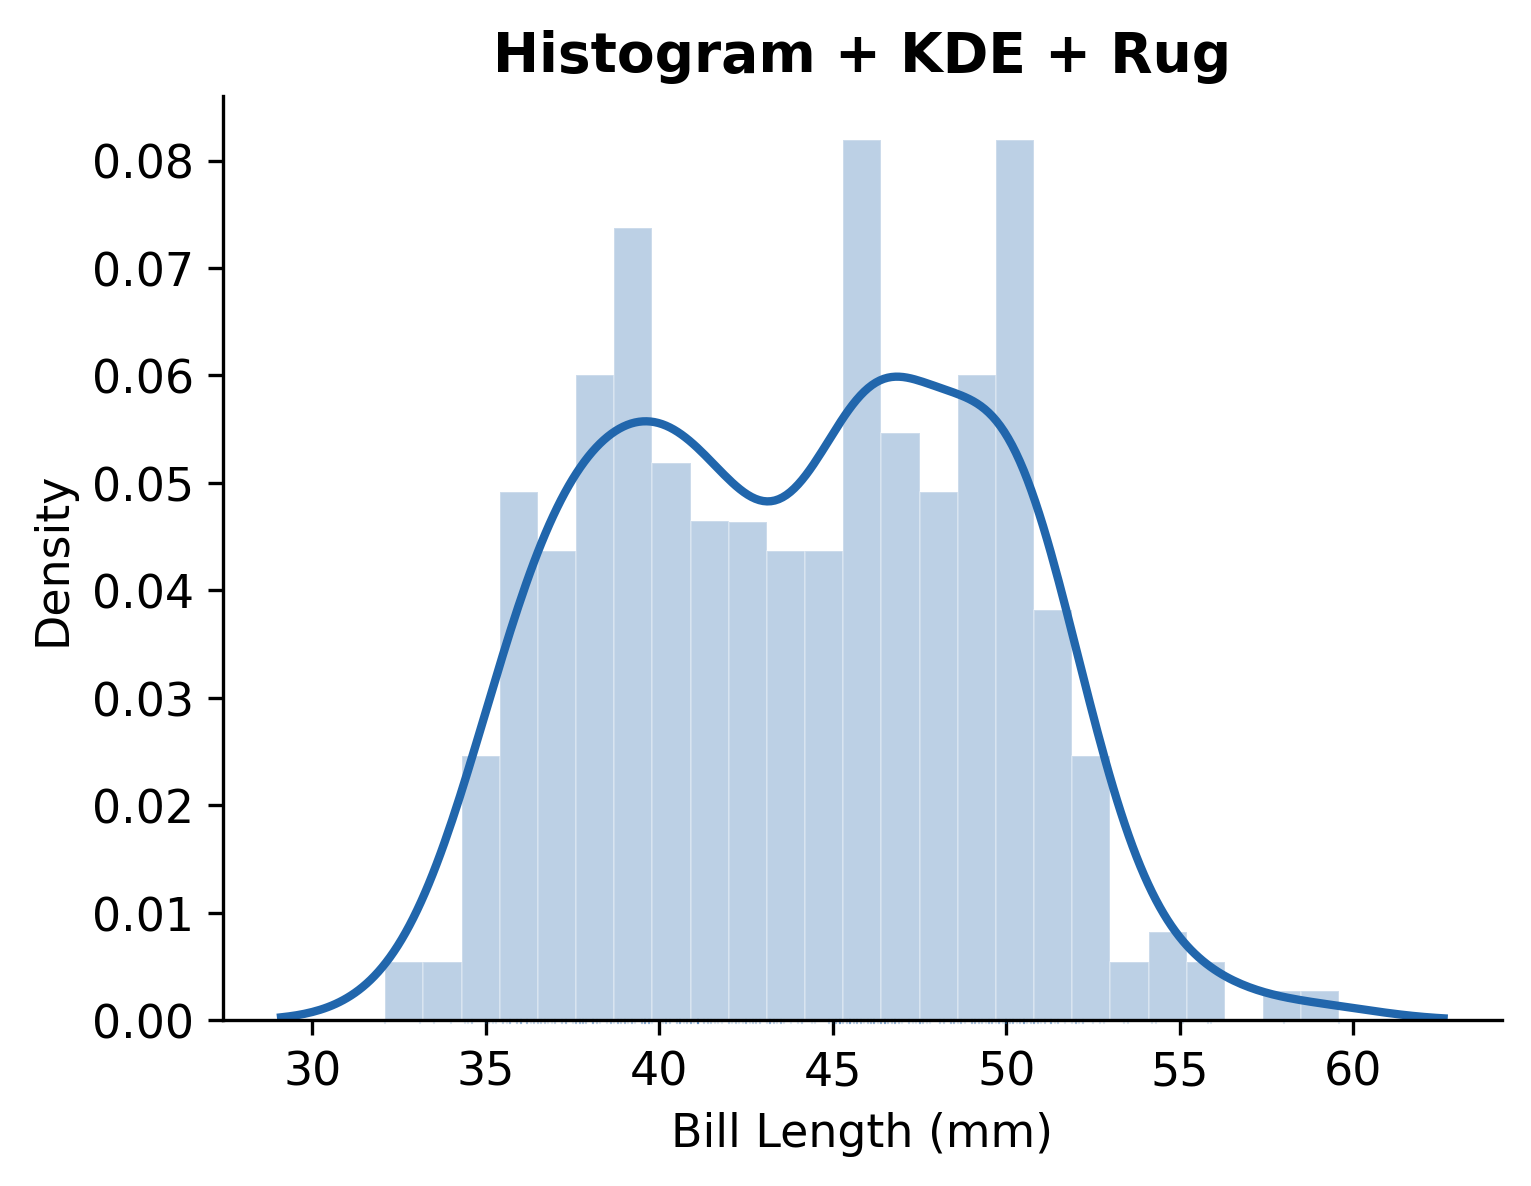
\includegraphics[width=\textwidth]{m1_4_hist_kde_rug.png}
\begin{exampleblock}{Data Insight}
    \scriptsize \texttt{sns.histplot(kde=True)} adds the KDE automatically. Add \texttt{plt.rug()} for the third layer.
\end{exampleblock}
\end{column}
\end{columns}
\end{frame}

% ── 107 ──
\begin{frame}{Grouped Distributions: Stacked vs.\ Overlaid}
\smark{107/300}
\centering
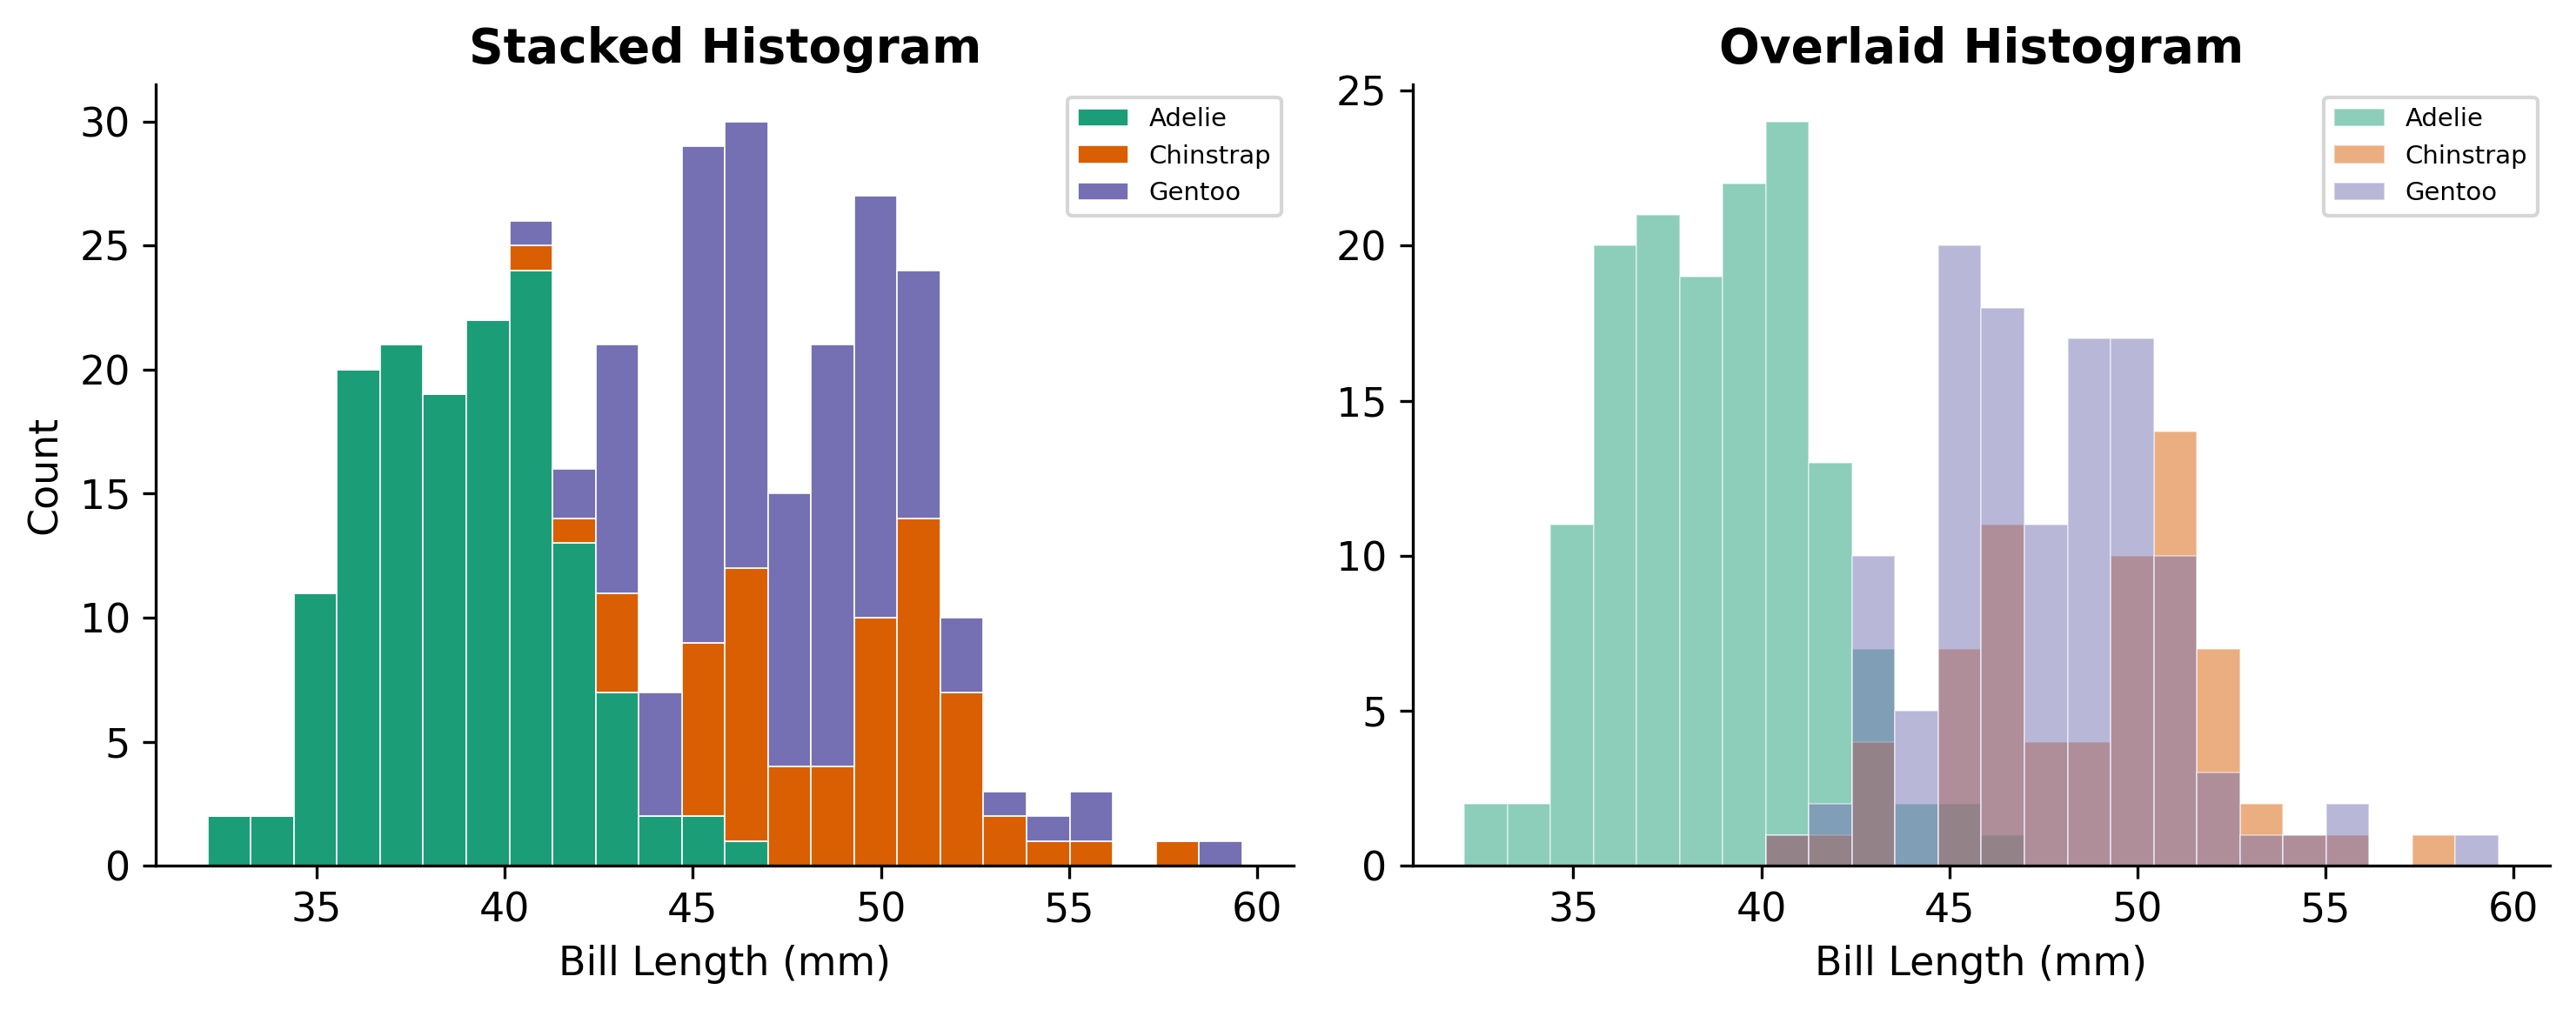
\includegraphics[width=0.85\textwidth]{m1_4_hist_grouped.png}

\vspace{0.2cm}
\begin{columns}[T]
\begin{column}{0.48\textwidth}
\begin{exampleblock}{Data Insight}
    \scriptsize \textbf{Stacked} preserves totals but hides individual shapes. \textbf{Overlaid} shows shapes but occludes. Best alternative: use \texttt{geom\_density()} or facets.
\end{exampleblock}
\end{column}
\begin{column}{0.48\textwidth}
\begin{alertblock}{Pro-Tip}
    \scriptsize For 3+ groups, \textbf{overlaid histograms fail}. Switch to density curves or faceted panels (slide 117).
\end{alertblock}
\end{column}
\end{columns}
\end{frame}

% ── 108 ──
\begin{frame}[fragile]{Grouped Histogram --- \Rlang}\smark{108/300}
\begin{columns}[T]
\begin{column}{0.55\textwidth}
\begin{lstlisting}[style=Rstyle]
# Stacked (default)
ggplot(penguins,
  aes(bill_length_mm,
      fill = species)) +
  geom_histogram(bins = 25,
    color = "white") +
  scale_fill_manual(
    values=c("#1B9E77","#D95F02",
             "#7570B3"))

# Overlaid (identity + alpha)
ggplot(penguins,
  aes(bill_length_mm,
      fill = species)) +
  geom_histogram(bins = 25,
    position = "identity",
    alpha = 0.4, color="white")
\end{lstlisting}
\end{column}
\begin{column}{0.42\textwidth}
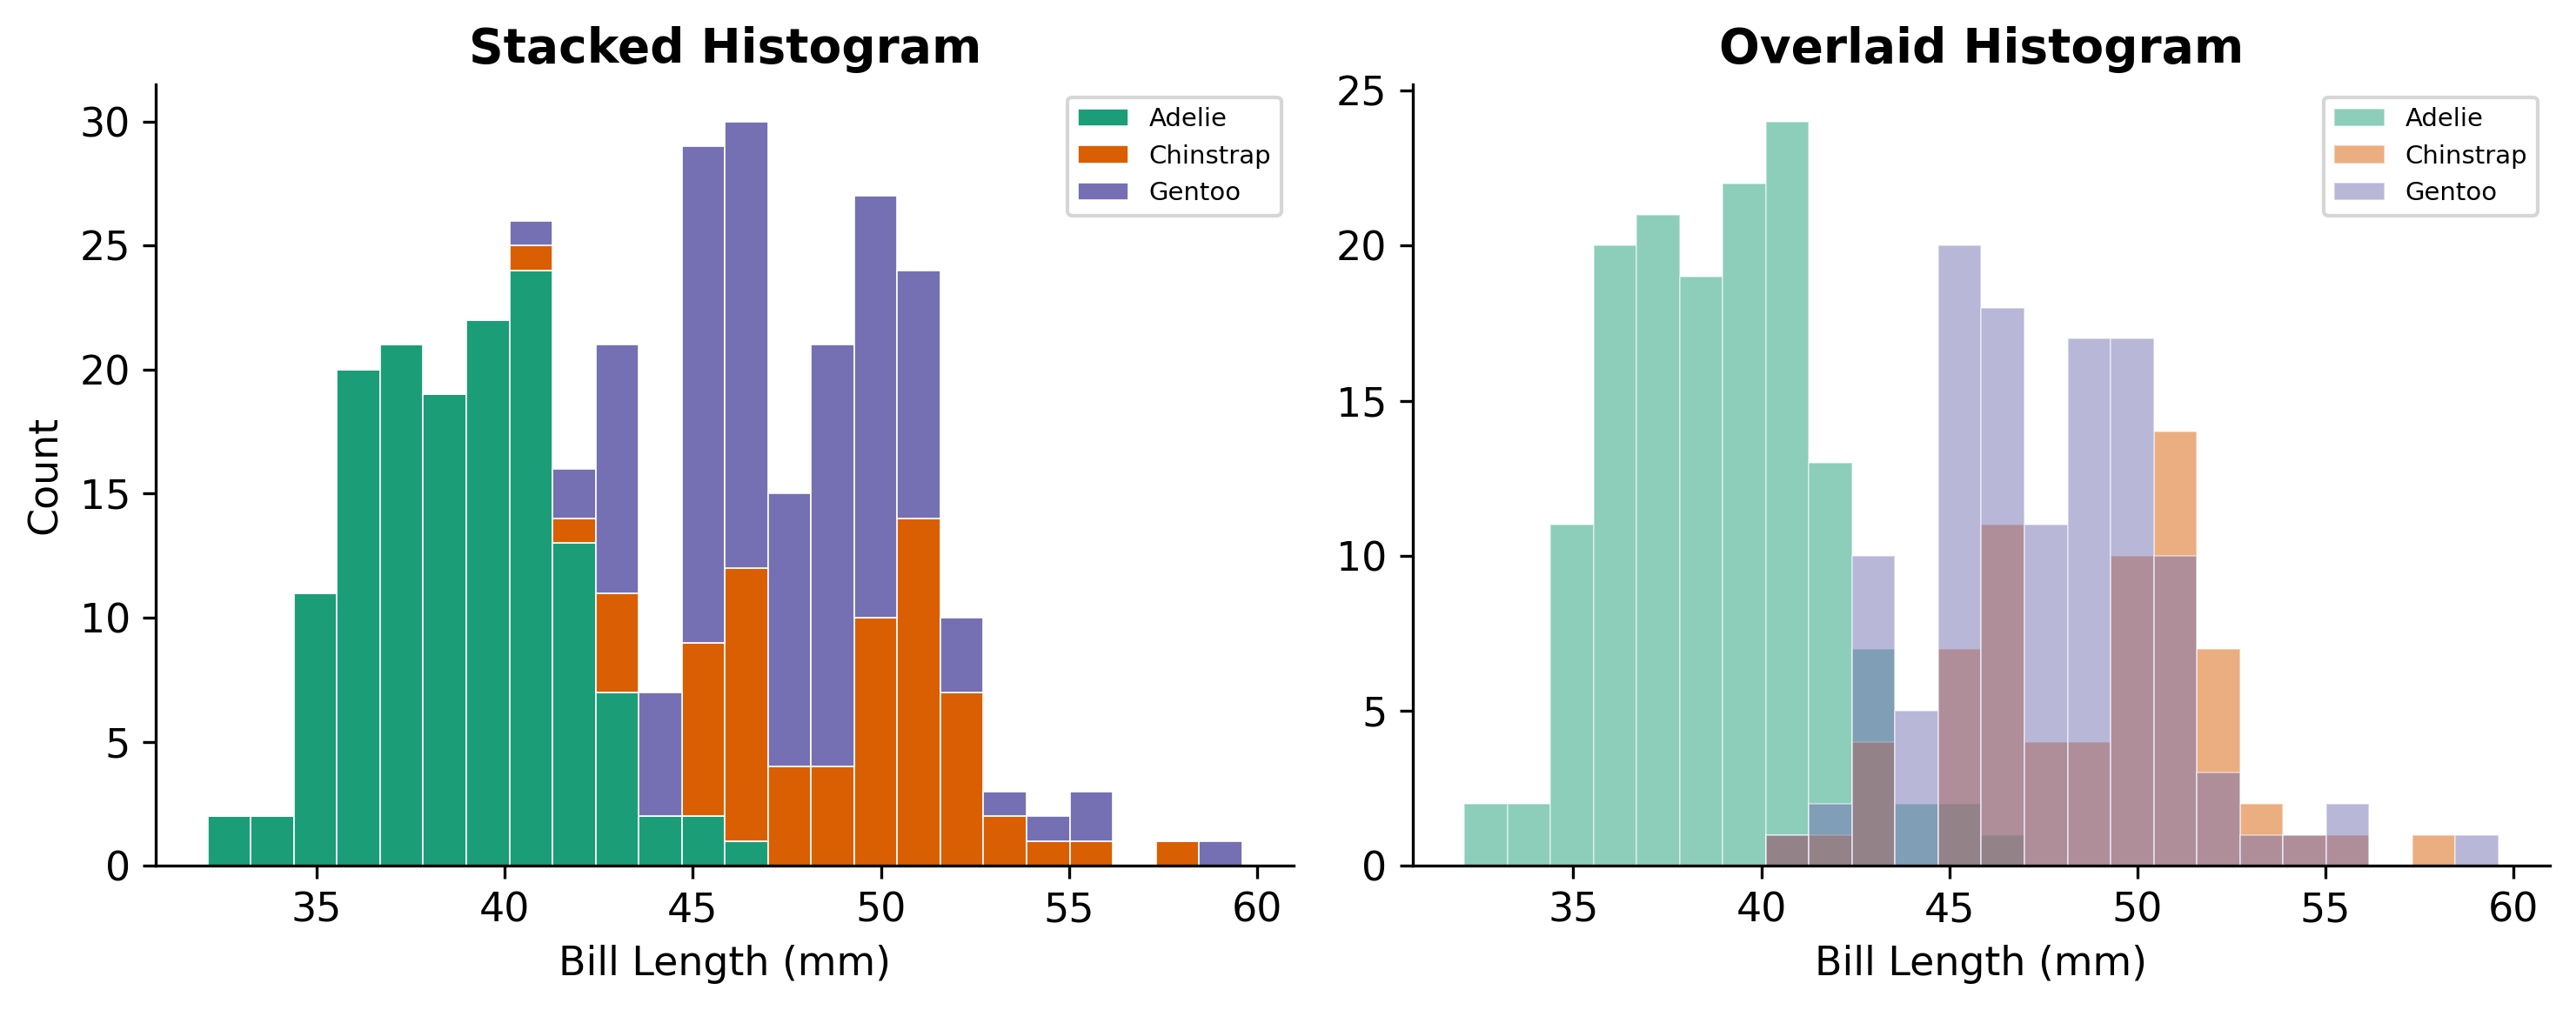
\includegraphics[width=\textwidth]{m1_4_hist_grouped.png}
\end{column}
\end{columns}
\end{frame}

% ── 109 ──
\begin{frame}[fragile]{Grouped Histogram --- \Python}\smark{109/300}
\begin{columns}[T]
\begin{column}{0.55\textwidth}
\begin{lstlisting}[style=Pystyle]
# plotnine: stacked
(ggplot(penguins,
   aes("bill_length_mm",
       fill="species"))
 + geom_histogram(bins=25,
     color="white"))

# matplotlib: overlaid
for sp, c in zip(species, colors):
    sub = pen[pen["species"]==sp]
    plt.hist(sub["bill_length_mm"],
      bins=25, alpha=0.4, color=c,
      label=sp)
plt.legend()
\end{lstlisting}
\end{column}
\begin{column}{0.42\textwidth}
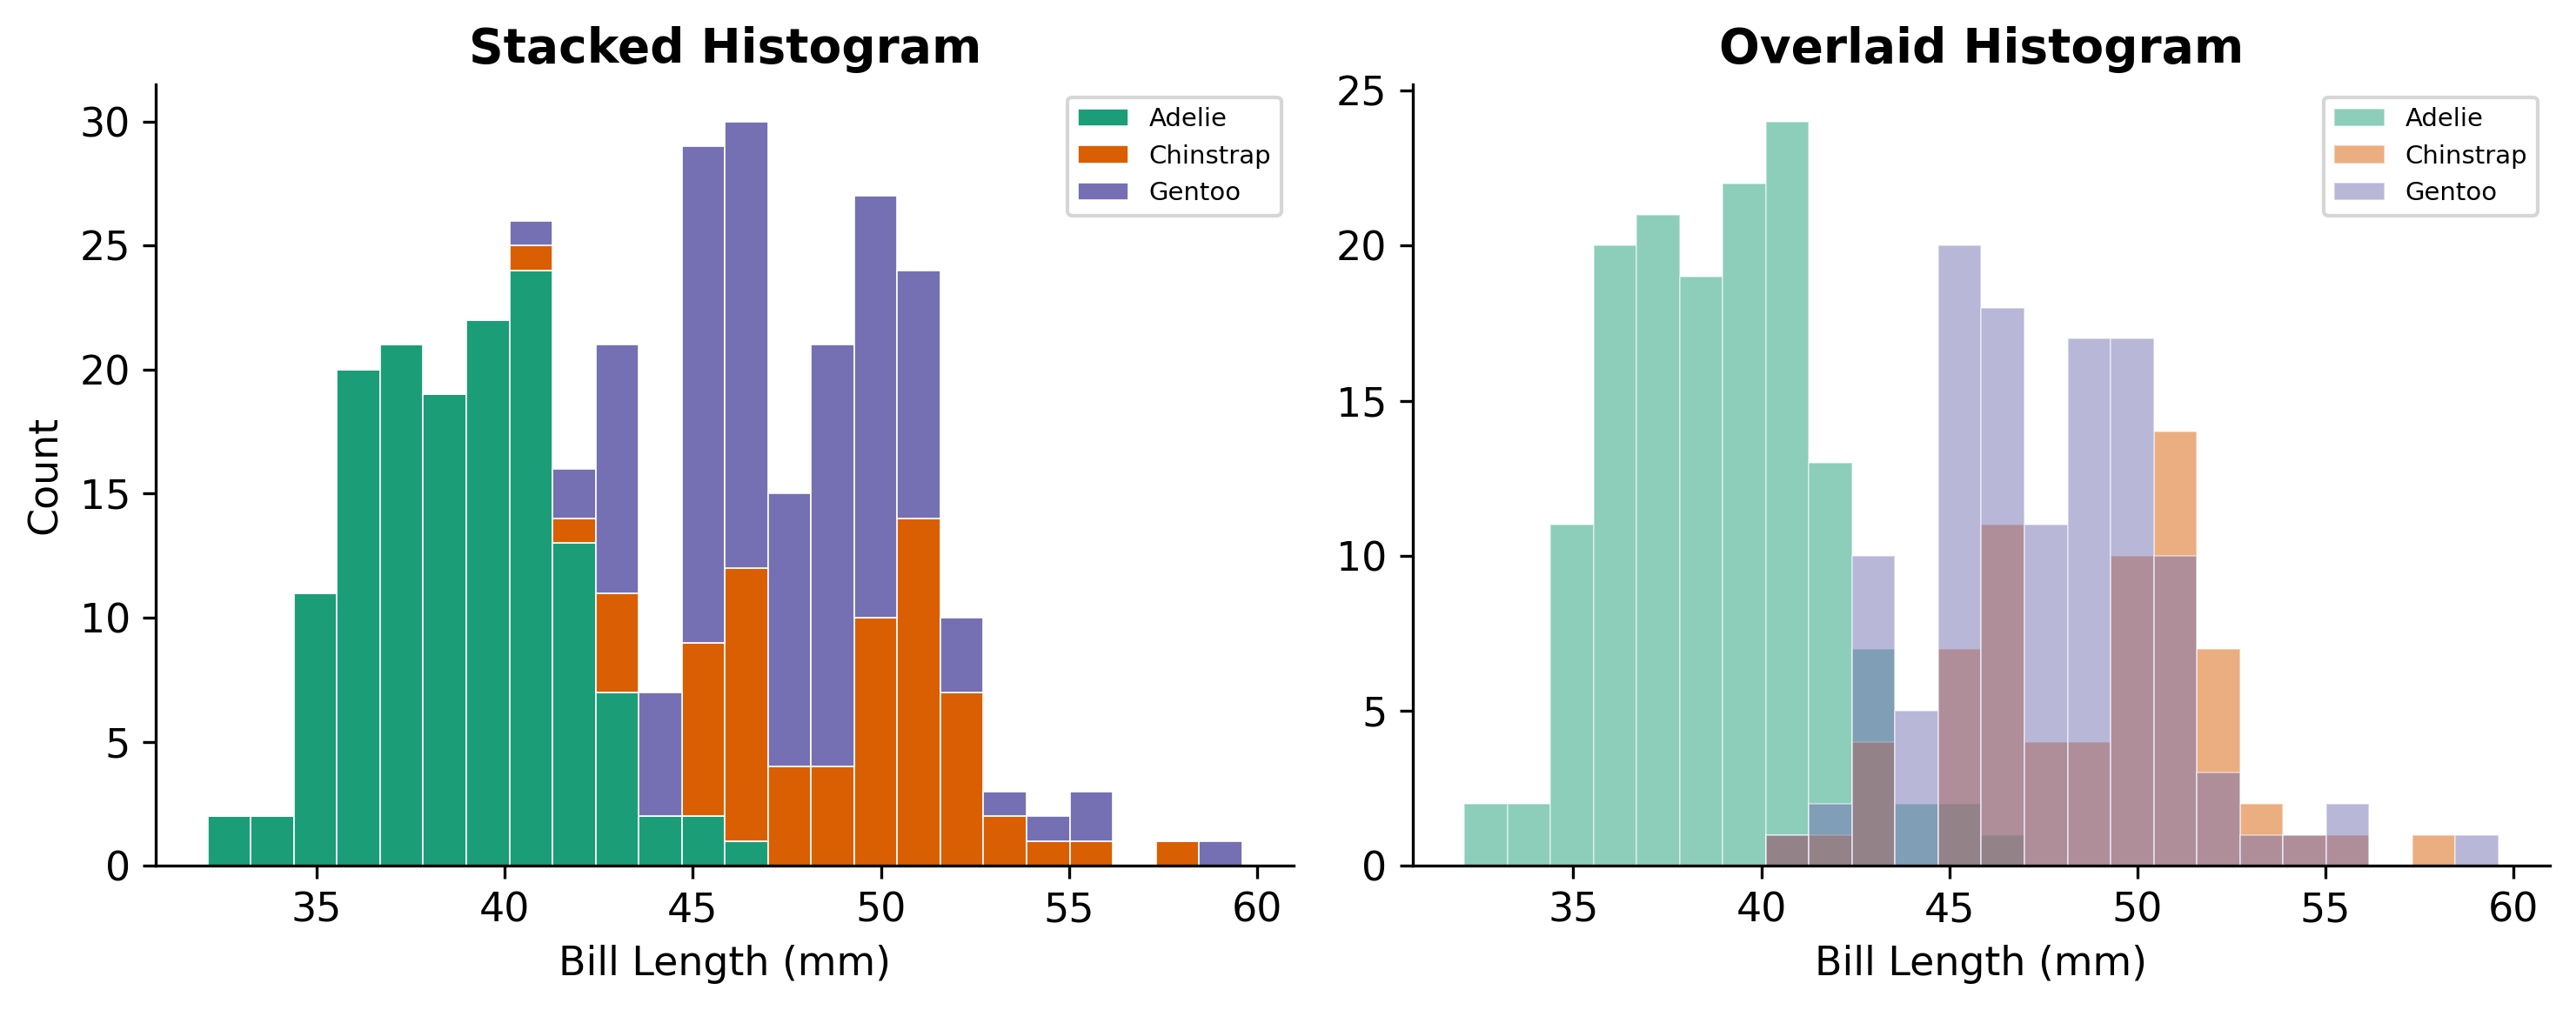
\includegraphics[width=\textwidth]{m1_4_hist_grouped.png}
\begin{alertblock}{Pro-Tip}
    \scriptsize In plotnine, add \texttt{position="identity"} + \texttt{alpha} for overlaid. Default is \texttt{position="stack"}.
\end{alertblock}
\end{column}
\end{columns}
\end{frame}

% ── 110 ──
\begin{frame}{Grouped Density Curves}
\smark{110/300}
\begin{columns}[T]
\begin{column}{0.50\textwidth}
\begin{itemize}
    \item The cleanest way to compare 2--5 distributions on one axis
    \item No occlusion problems (fill with low alpha)
    \item Each curve integrates to 1 (comparable even if group $n$ differs)
    \item Preferred over overlaid histograms
\end{itemize}
\end{column}
\begin{column}{0.47\textwidth}
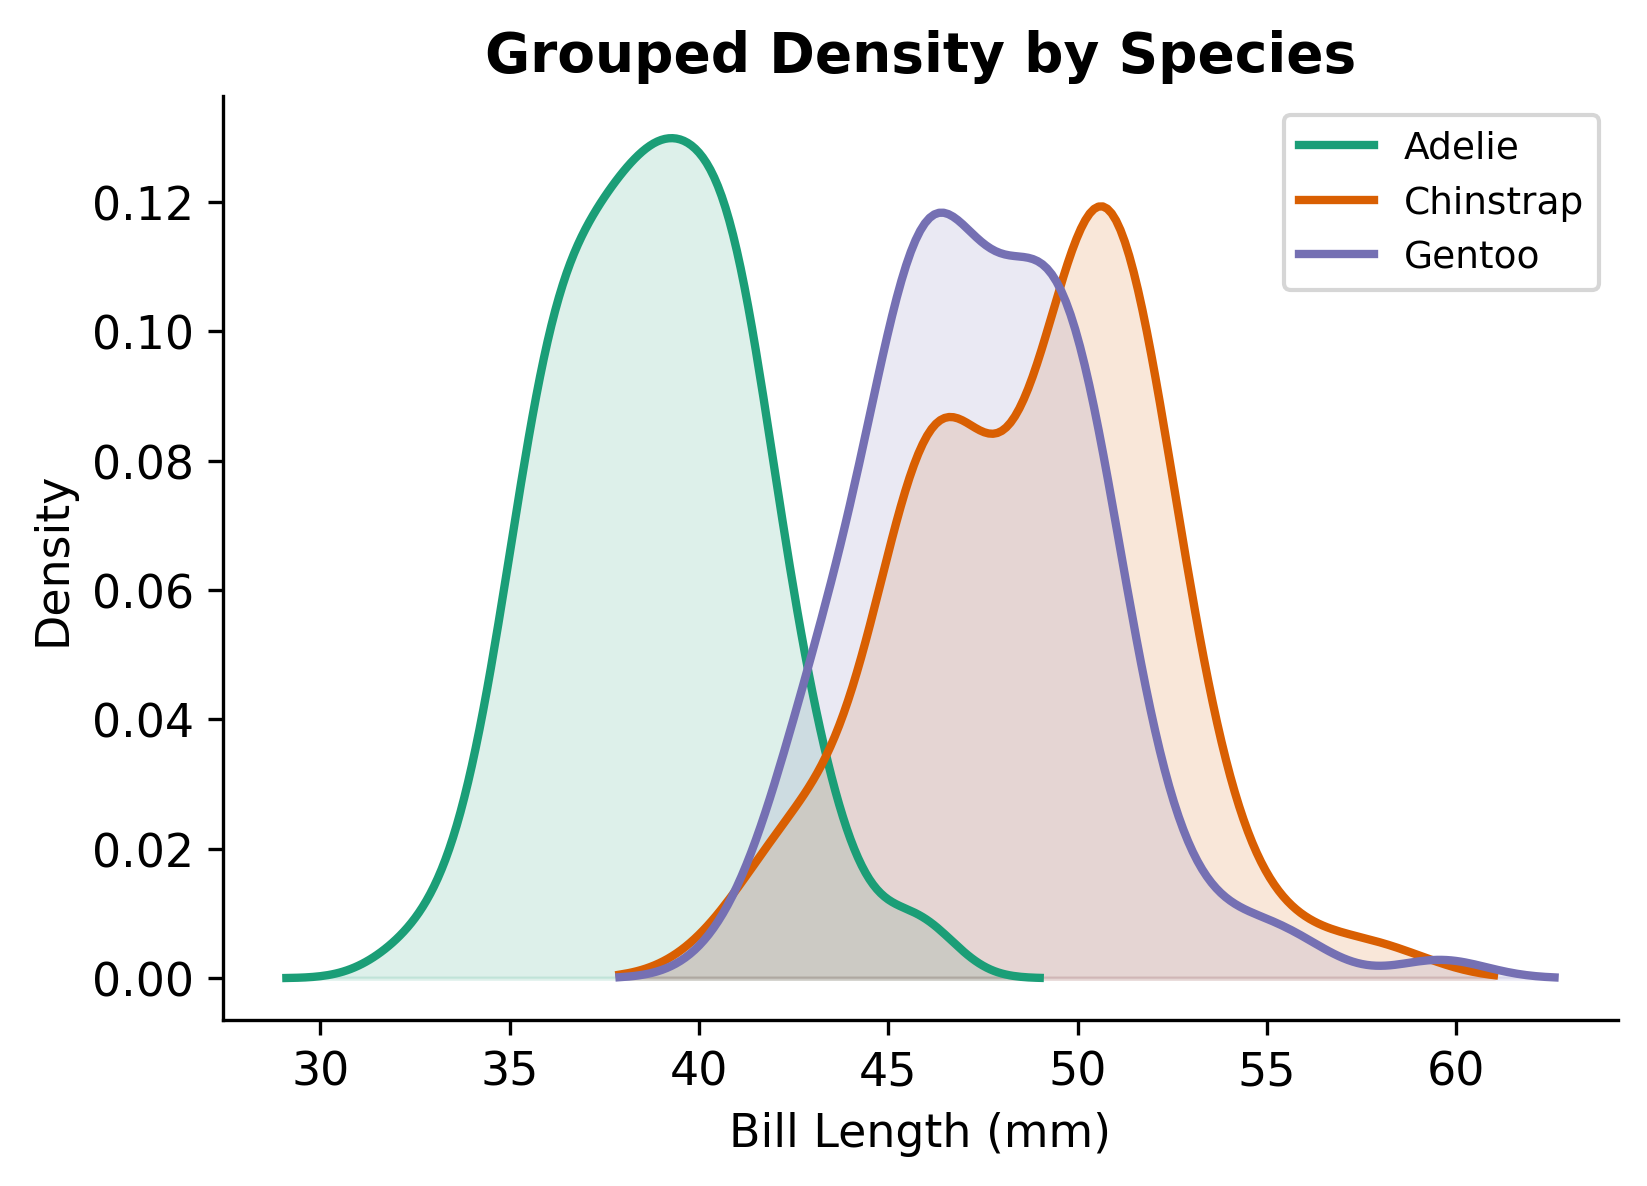
\includegraphics[width=\textwidth]{m1_4_density_grouped.png}
\begin{exampleblock}{Data Insight}
    \scriptsize Adelie is clearly separated from Chinstrap/Gentoo. The overlap between Chinstrap and Gentoo suggests harder classification.
\end{exampleblock}
\end{column}
\end{columns}
\end{frame}

% ── 111 ──
\begin{frame}[fragile]{Grouped Density --- \Rlang}\smark{111/300}
\begin{columns}[T]
\begin{column}{0.55\textwidth}
\begin{lstlisting}[style=Rstyle]
ggplot(penguins,
  aes(bill_length_mm,
      fill = species,
      color = species)) +
  geom_density(alpha = 0.2) +
  scale_fill_manual(
    values=c("#1B9E77","#D95F02",
             "#7570B3")) +
  scale_color_manual(
    values=c("#1B9E77","#D95F02",
             "#7570B3")) +
  theme_minimal()
\end{lstlisting}
\end{column}
\begin{column}{0.42\textwidth}
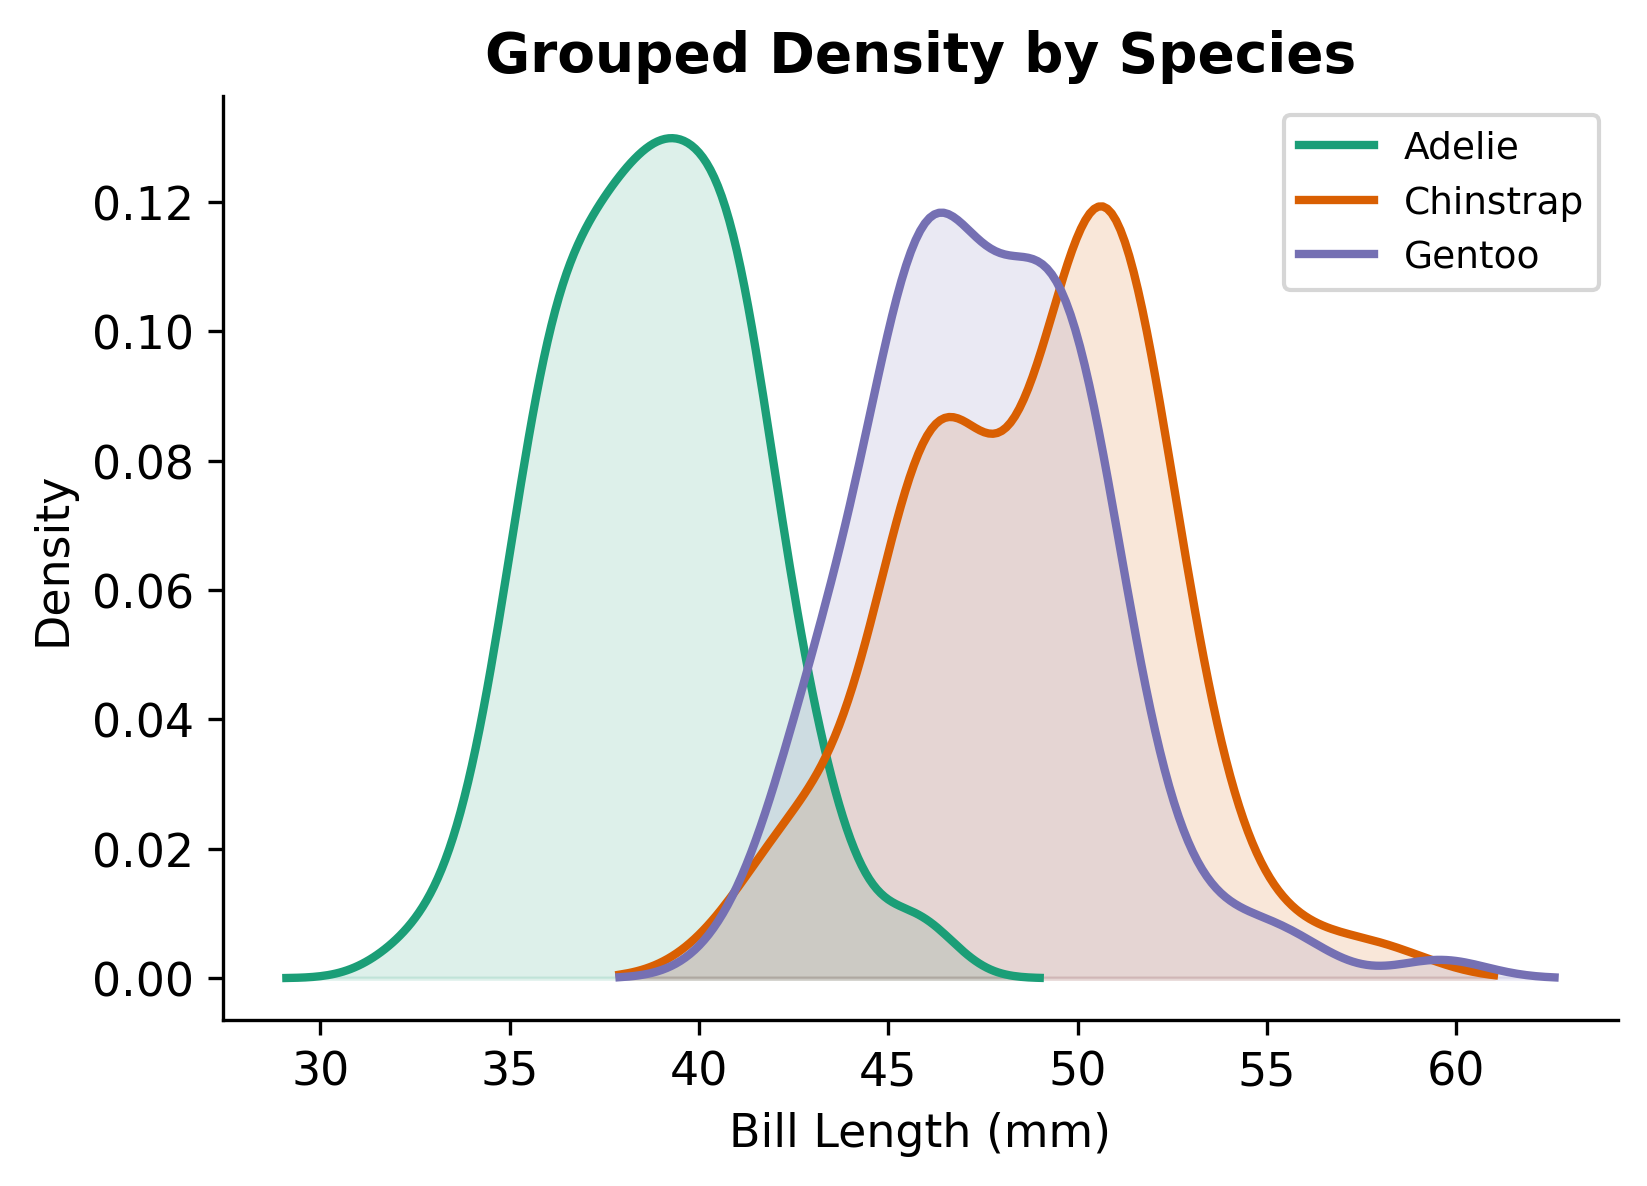
\includegraphics[width=\textwidth]{m1_4_density_grouped.png}
\end{column}
\end{columns}
\end{frame}

% ── 112 ──
\begin{frame}[fragile]{Grouped Density --- \Python}\smark{112/300}
\begin{columns}[T]
\begin{column}{0.55\textwidth}
\begin{lstlisting}[style=Pystyle]
# plotnine
(ggplot(penguins,
   aes("bill_length_mm",
       fill="species",
       color="species"))
 + geom_density(alpha=0.2))

# seaborn
sns.kdeplot(data=penguins,
    x="bill_length_mm",
    hue="species",
    fill=True, alpha=0.2,
    common_norm=False)
\end{lstlisting}
\end{column}
\begin{column}{0.42\textwidth}
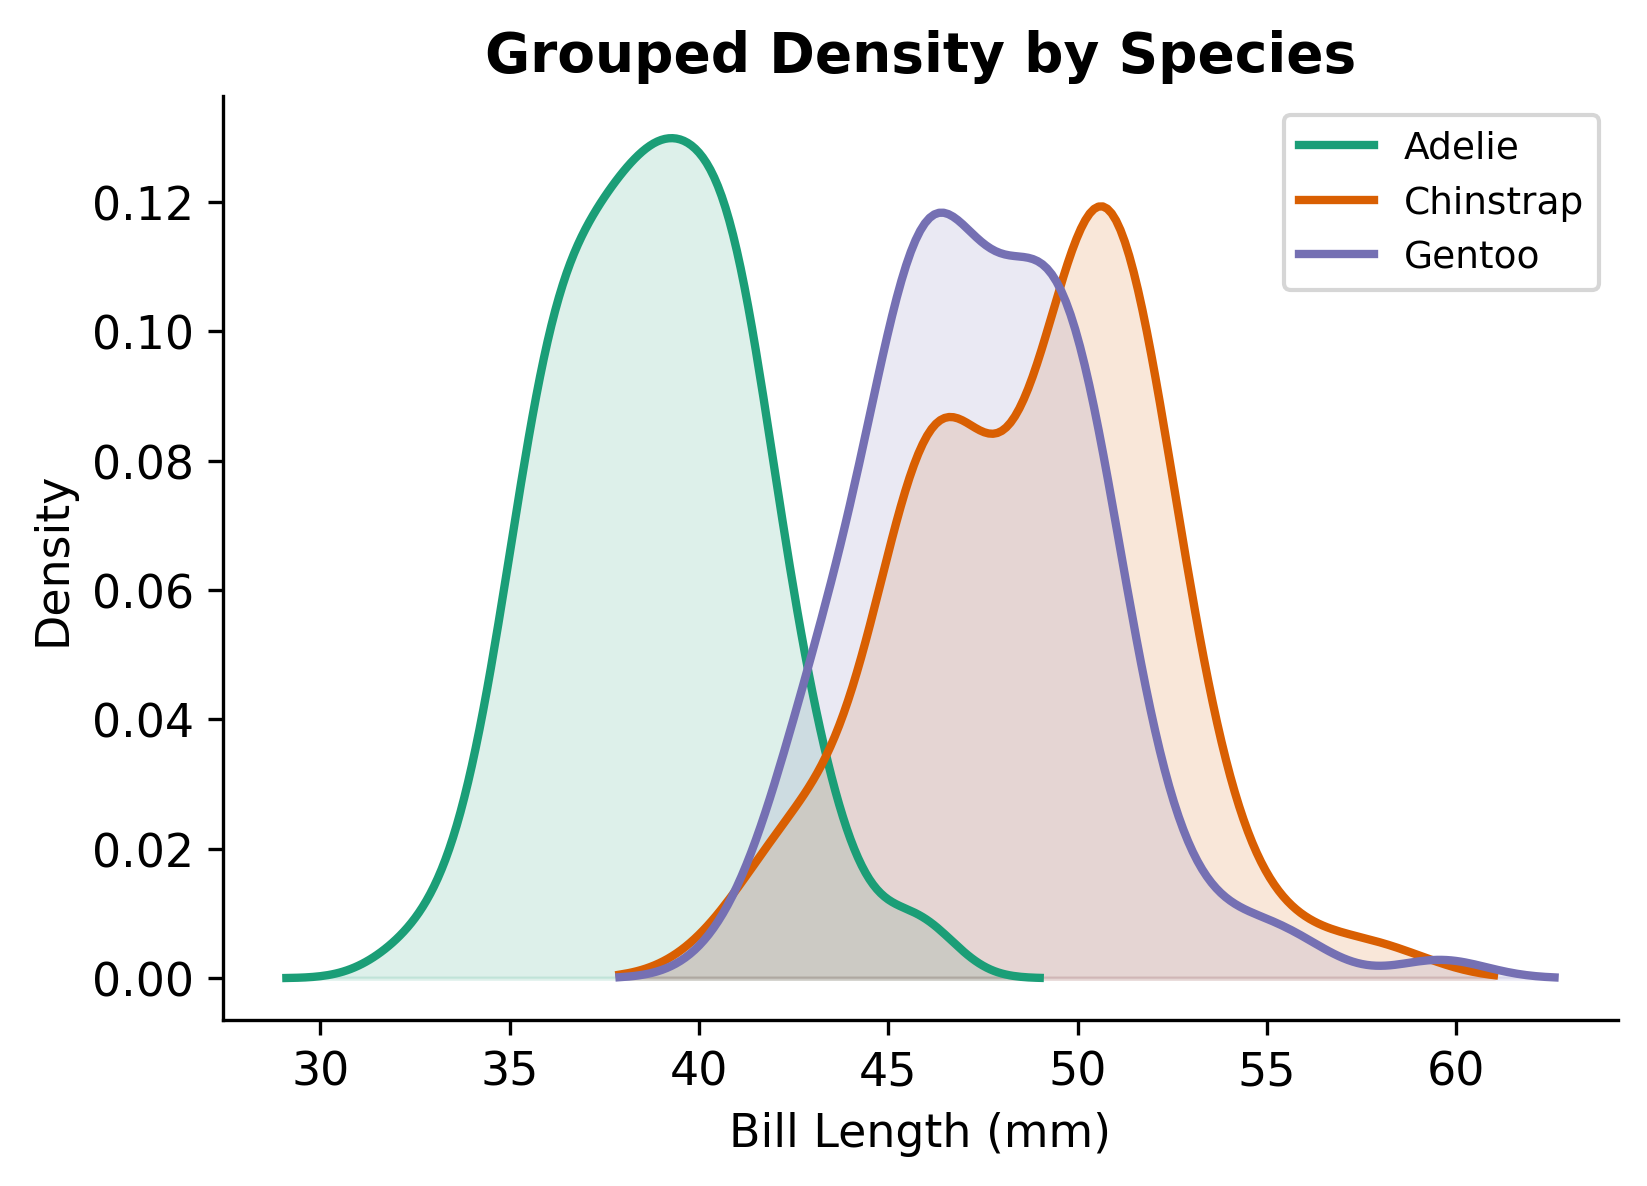
\includegraphics[width=\textwidth]{m1_4_density_grouped.png}
\begin{alertblock}{Pro-Tip}
    \scriptsize \texttt{common\_norm=False} in seaborn ensures each group integrates to 1 independently. Default (\texttt{True}) normalizes over the combined data.
\end{alertblock}
\end{column}
\end{columns}
\end{frame}

% ── 113 ──
\begin{frame}{QQ Plots: Assessing Distributional Fit}
\smark{113/300}
\begin{columns}[T]
\begin{column}{0.50\textwidth}
\begin{itemize}
    \item Plots observed quantiles vs.\ theoretical quantiles (usually normal)
    \item Points on the diagonal $\to$ data match the reference distribution
    \item Deviations reveal skew, heavy tails, outliers
    \item More powerful than histograms for normality assessment
\end{itemize}
\end{column}
\begin{column}{0.47\textwidth}
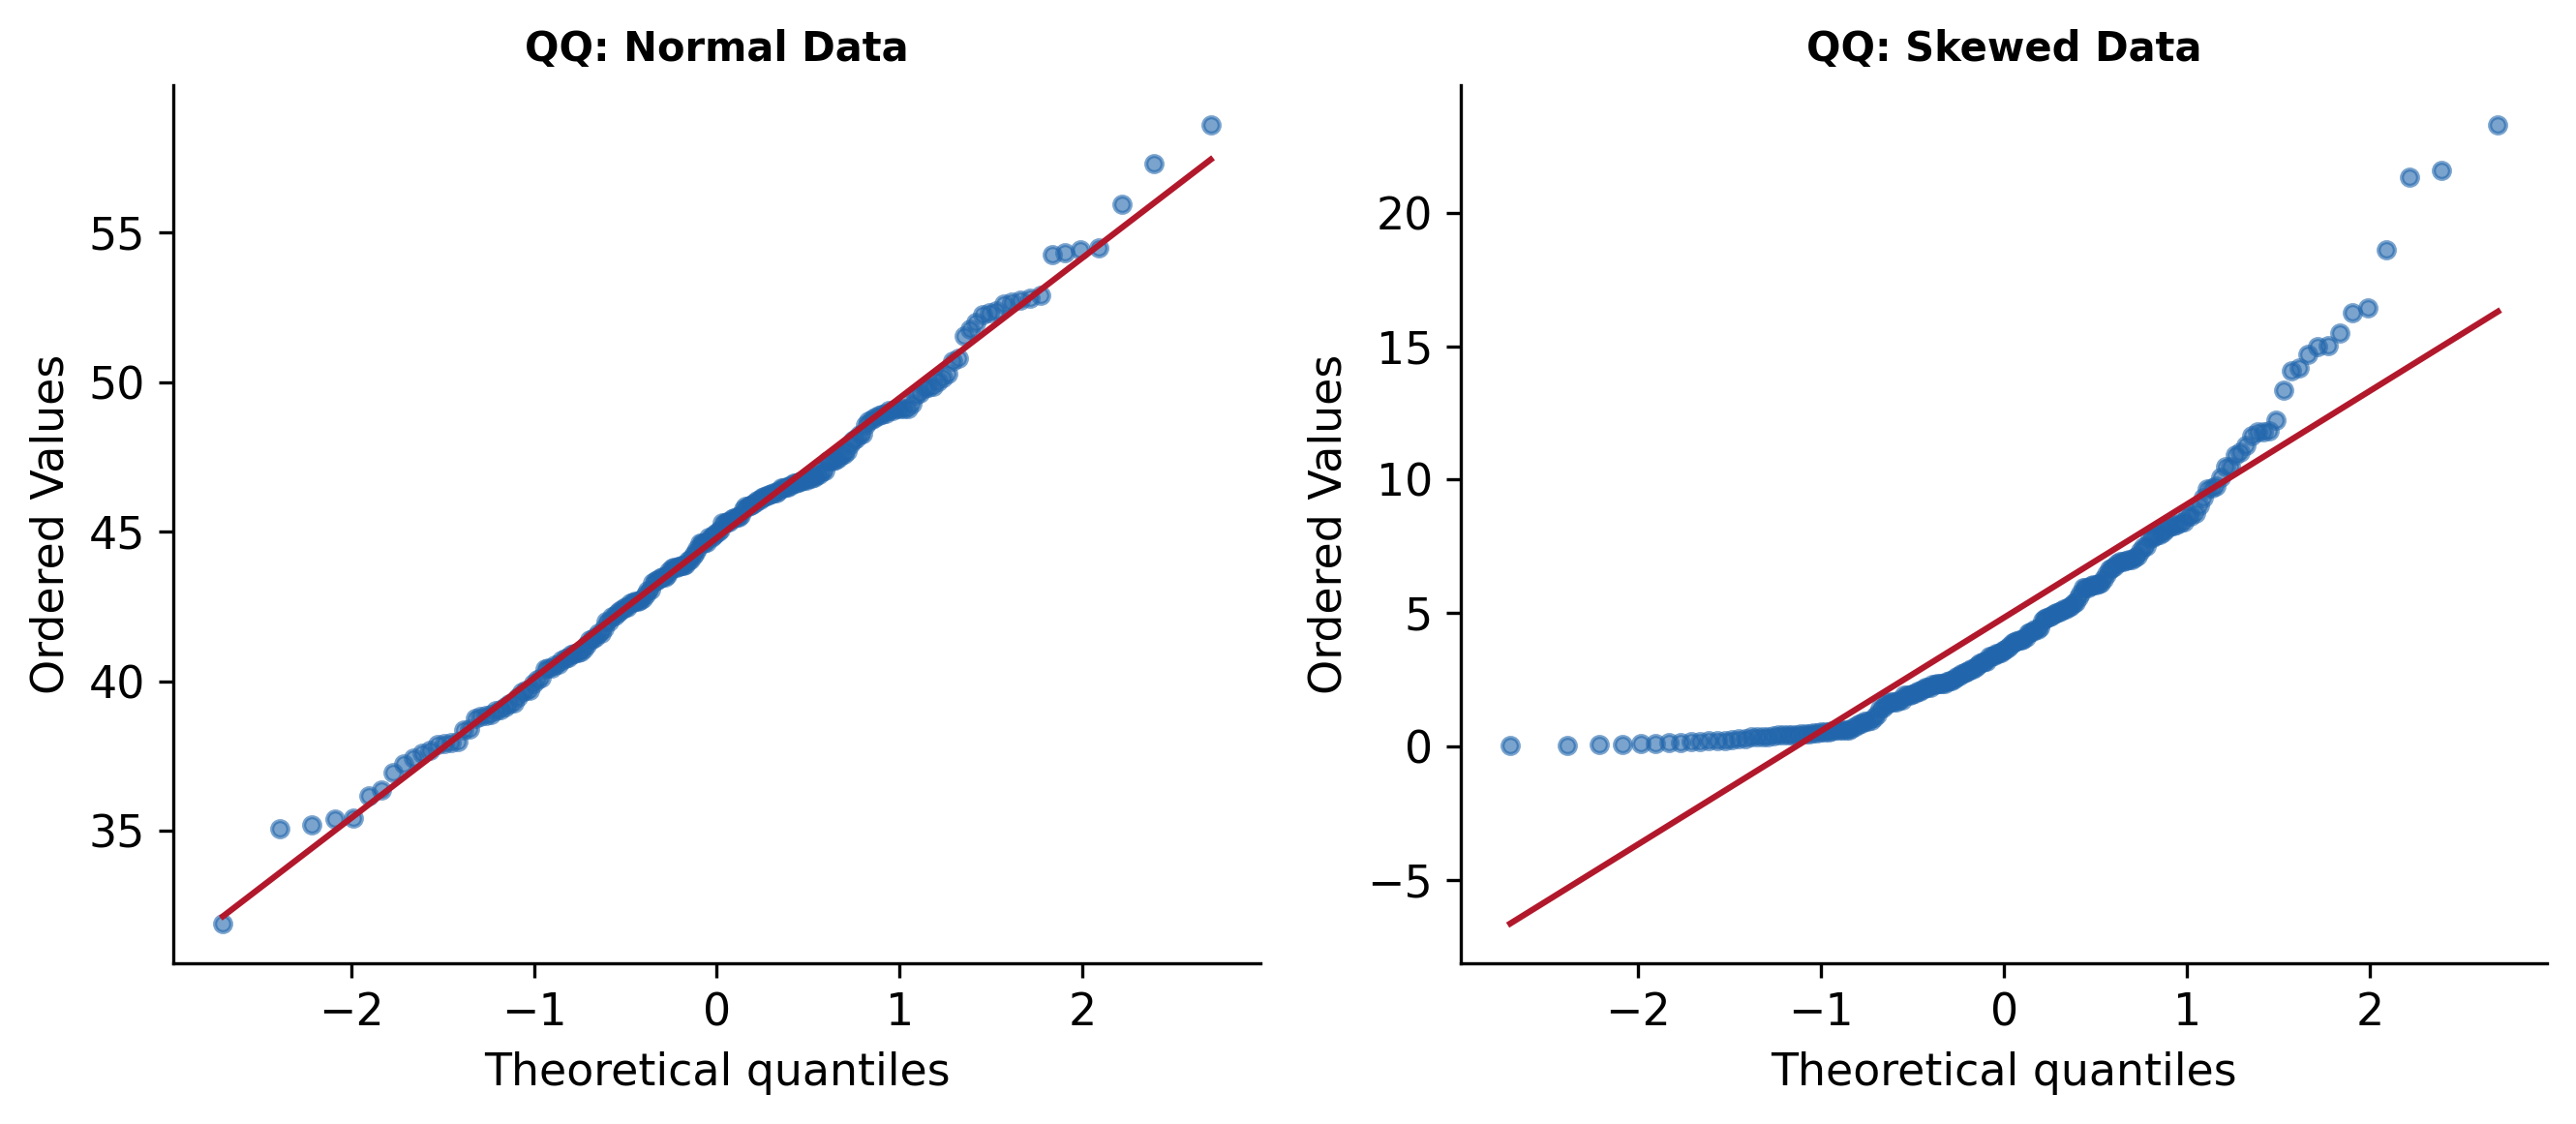
\includegraphics[width=\textwidth]{m1_4_qqplot.png}
\begin{exampleblock}{Data Insight}
    \scriptsize Left: normal data hugs the line. Right: exponential data curves away --- right skew is immediately visible.
\end{exampleblock}
\end{column}
\end{columns}
\end{frame}

% ── 114 ──
\begin{frame}[fragile]{QQ Plot --- \Rlang}\smark{114/300}
\begin{columns}[T]
\begin{column}{0.55\textwidth}
\begin{lstlisting}[style=Rstyle]
# Built-in QQ
ggplot(penguins,
  aes(sample = body_mass_g)) +
  geom_qq(color = "#2166AC") +
  geom_qq_line(color = "#B2182B",
    linewidth = 0.8) +
  labs(title = "QQ: Body Mass") +
  theme_minimal()

# Base R alternative
qqnorm(penguins$body_mass_g,
       pch = 19, col = "#2166AC")
qqline(penguins$body_mass_g,
       col = "#B2182B", lwd = 2)
\end{lstlisting}
\end{column}
\begin{column}{0.42\textwidth}
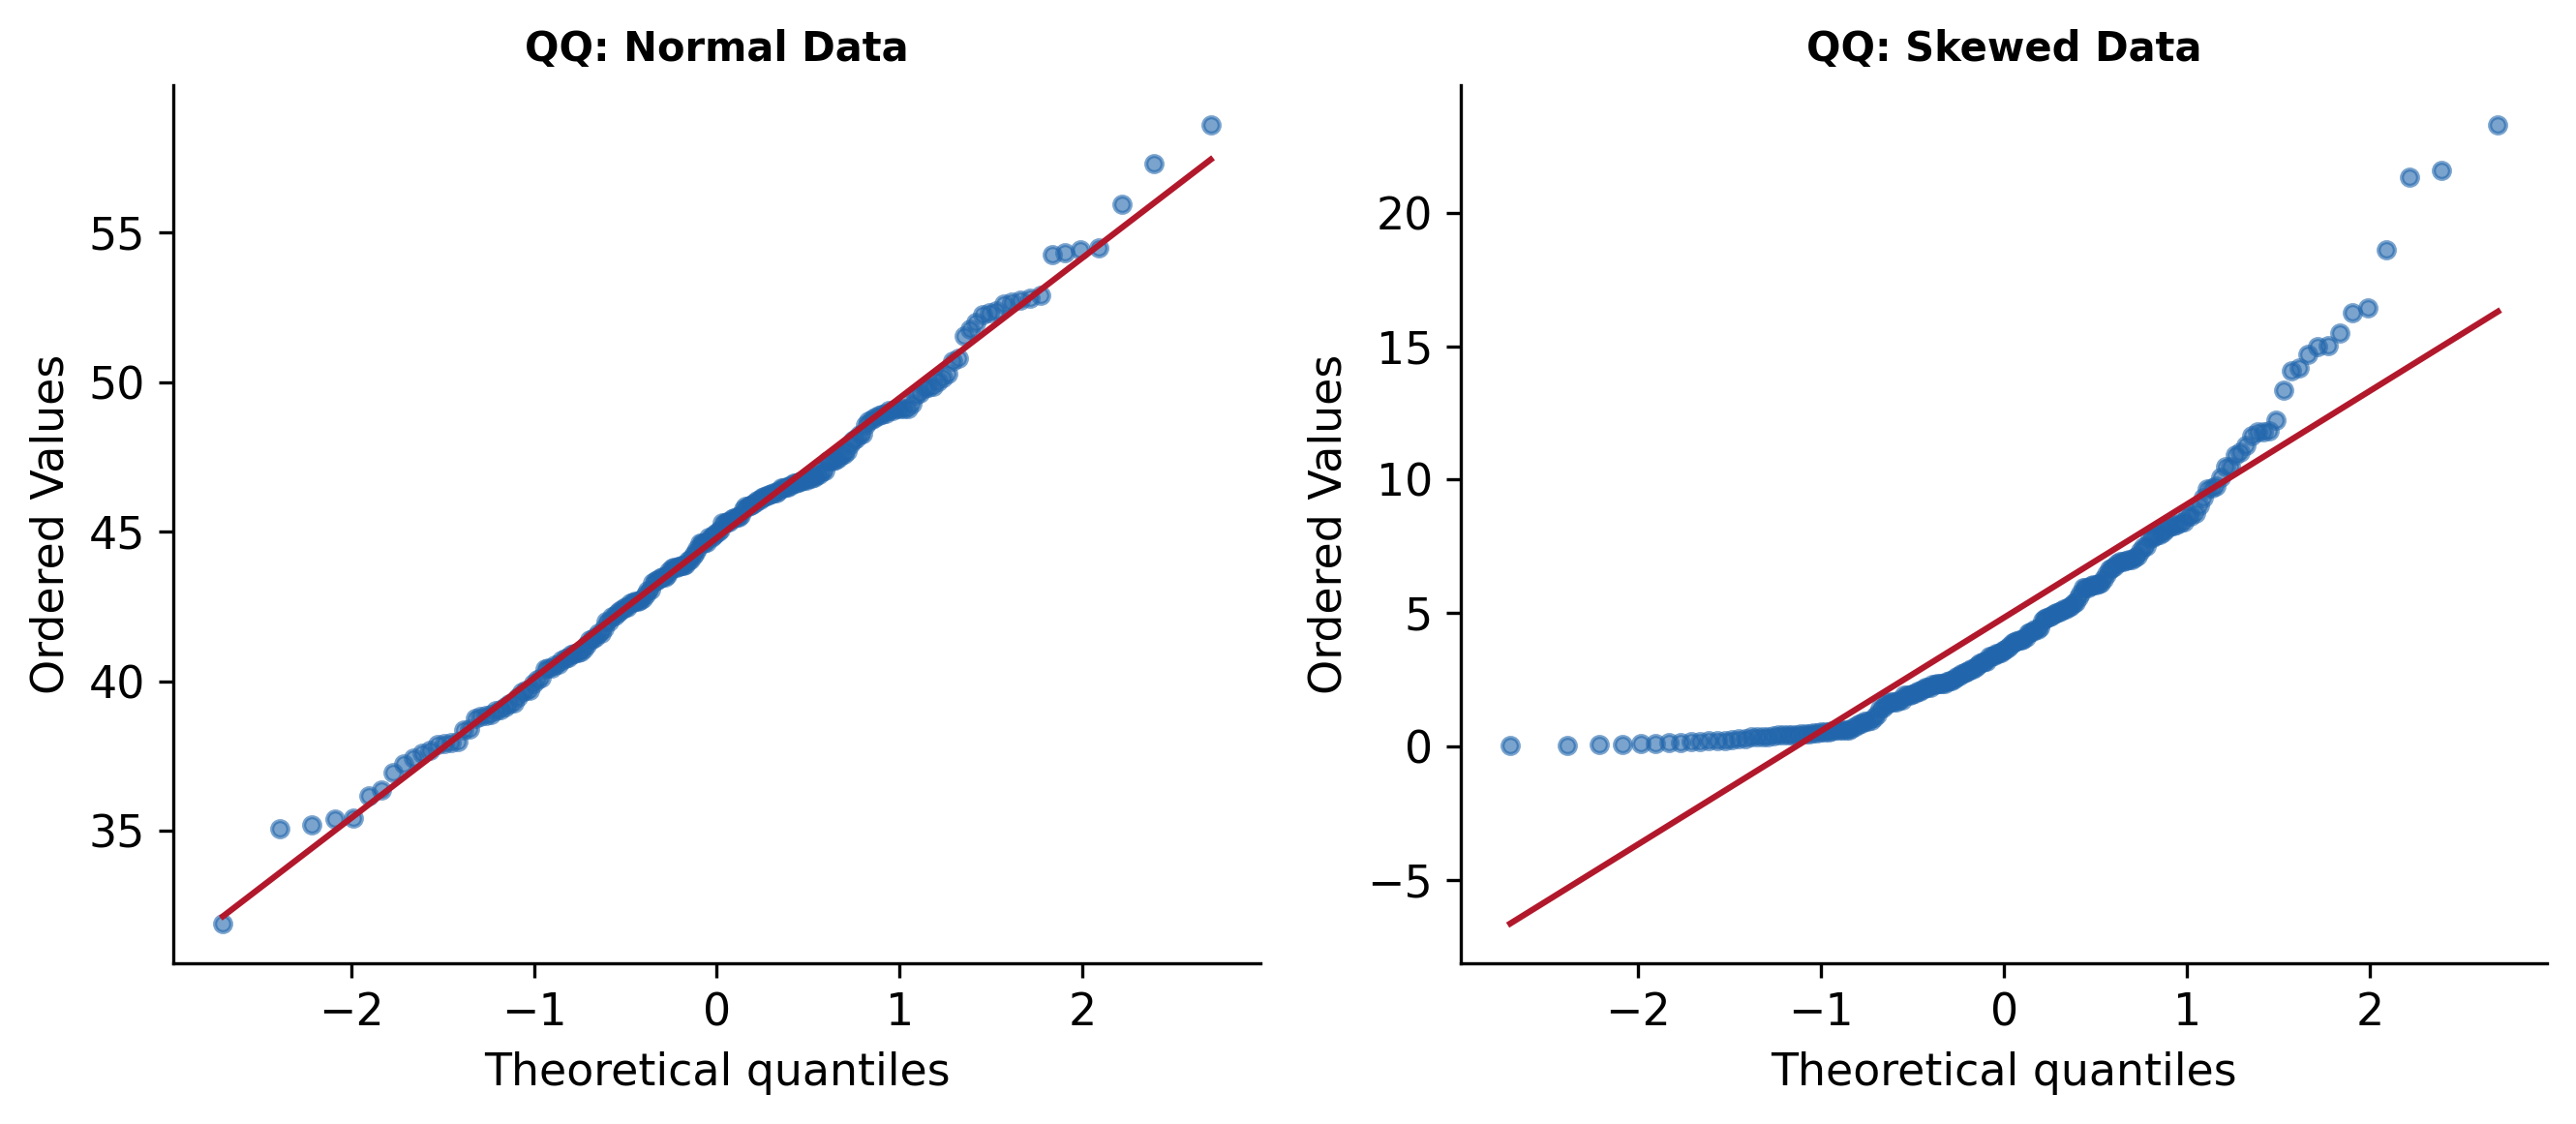
\includegraphics[width=\textwidth]{m1_4_qqplot.png}
\begin{alertblock}{Pro-Tip}
    \scriptsize \texttt{geom\_qq()} + \texttt{geom\_qq\_line()} use \texttt{aes(sample=)} --- not \texttt{x} and \texttt{y}.
\end{alertblock}
\end{column}
\end{columns}
\end{frame}

% ── 115 ──
\begin{frame}[fragile]{QQ Plot --- \Python}\smark{115/300}
\begin{columns}[T]
\begin{column}{0.55\textwidth}
\begin{lstlisting}[style=Pystyle]
from scipy import stats

# scipy.stats.probplot
fig, ax = plt.subplots()
stats.probplot(
    penguins["body_mass_g"],
    dist="norm", plot=ax)
ax.get_lines()[0].set(
    color="#B2182B", markersize=4)
ax.get_lines()[1].set(
    color="#2166AC", linewidth=1.5)
ax.set_title("QQ: Body Mass")

# plotnine
(ggplot(penguins,
   aes(sample="body_mass_g"))
 + geom_qq() + geom_qq_line())
\end{lstlisting}
\end{column}
\begin{column}{0.42\textwidth}
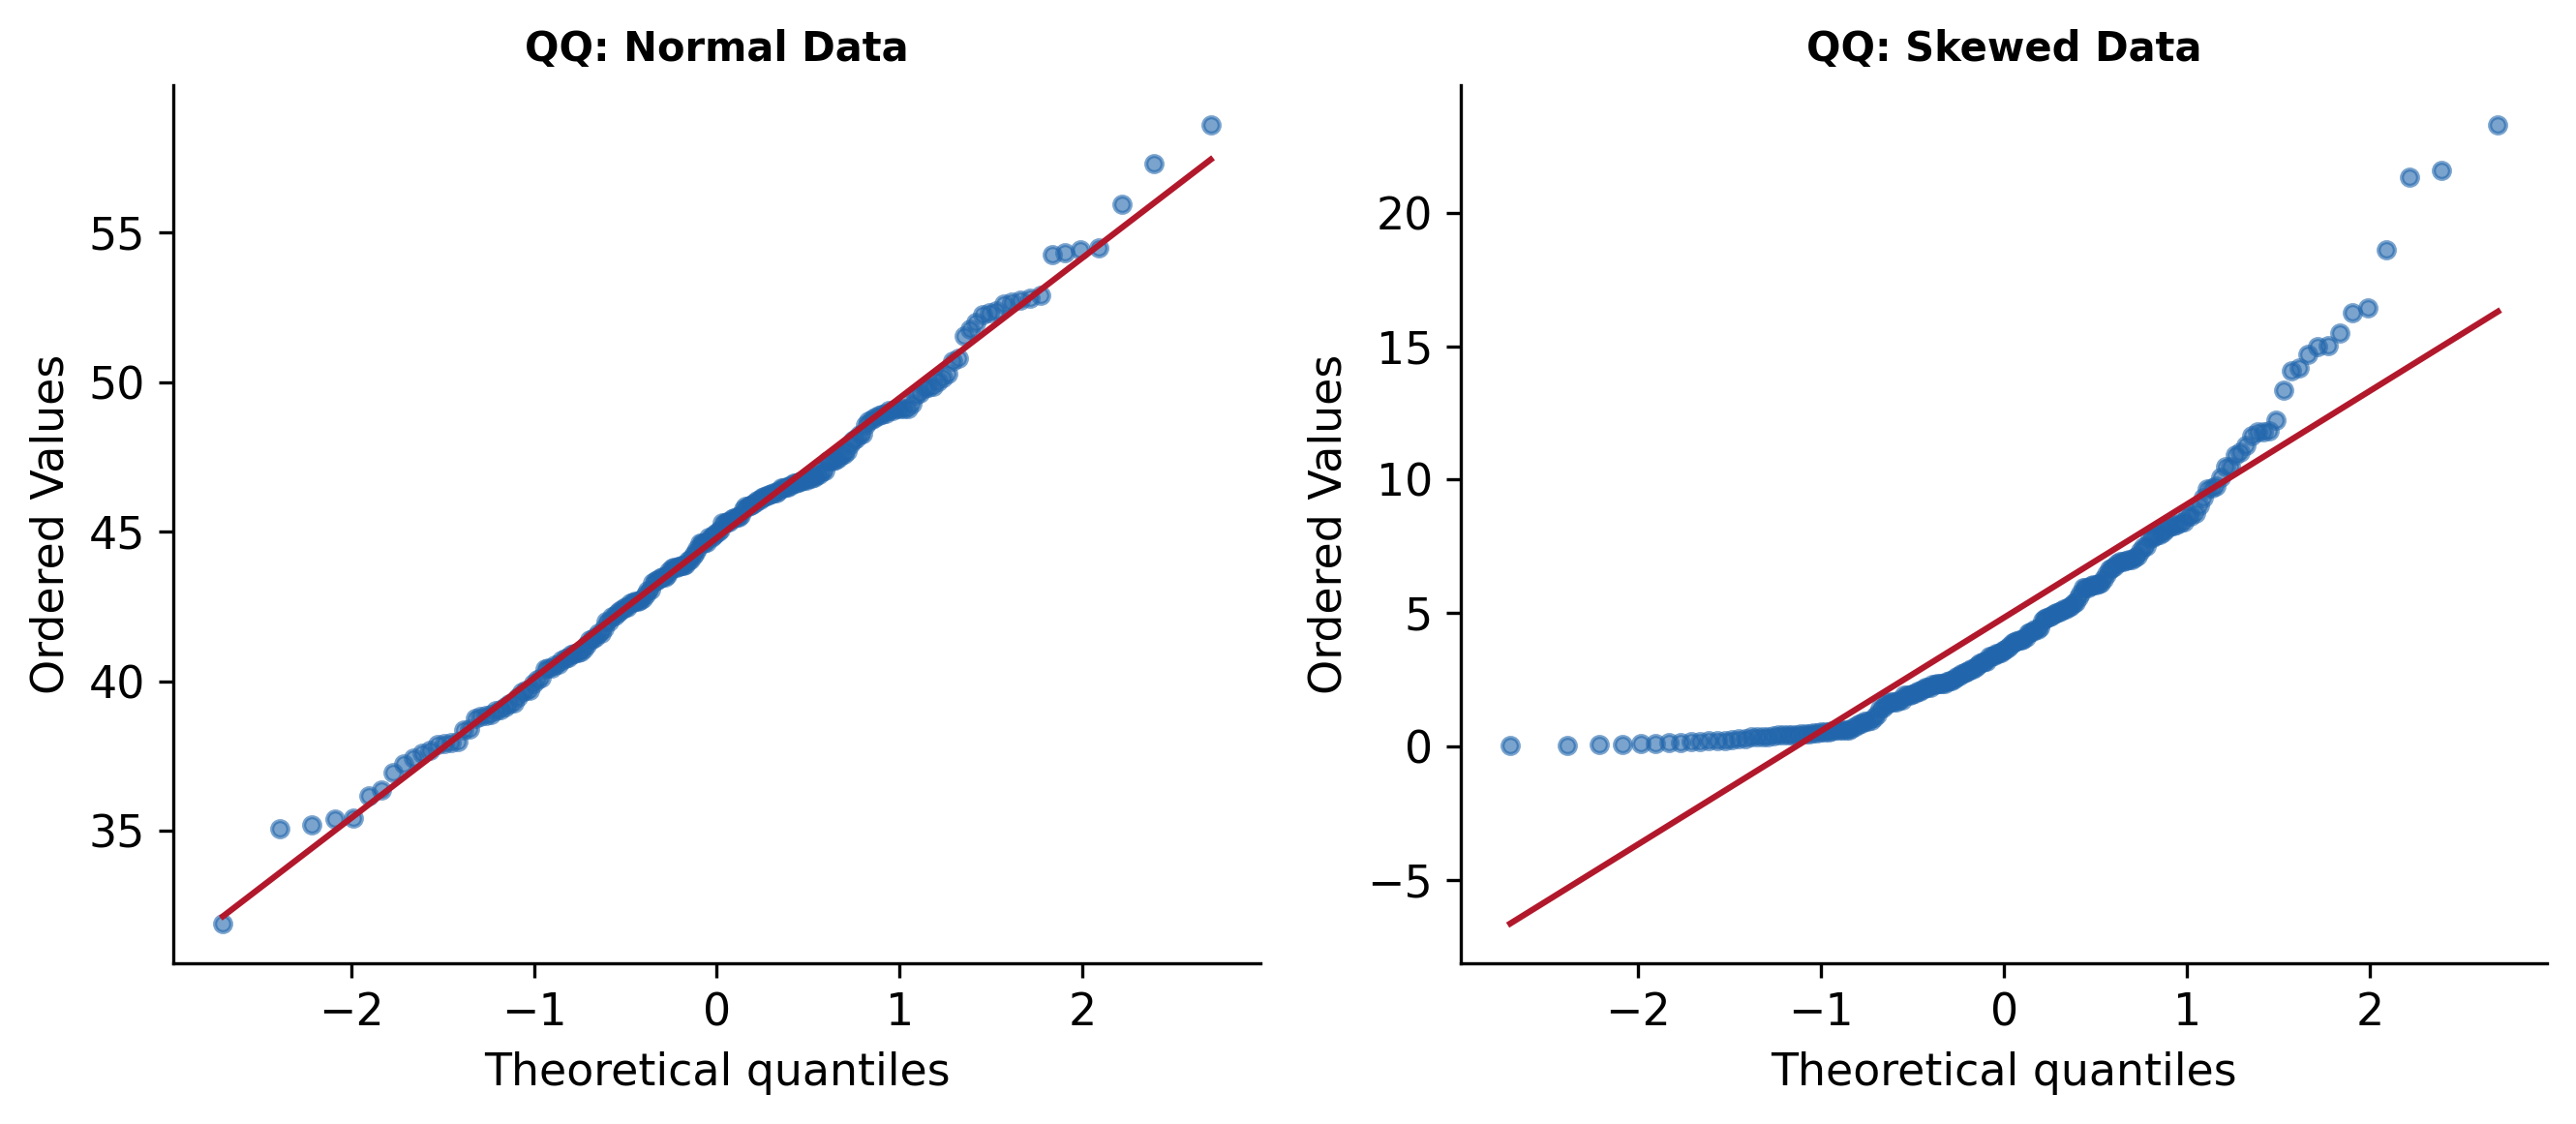
\includegraphics[width=\textwidth]{m1_4_qqplot.png}
\begin{exampleblock}{Data Insight}
    \scriptsize \texttt{scipy.stats.probplot()} is the Python workhorse. It computes theoretical quantiles and plots them against sorted data.
\end{exampleblock}
\end{column}
\end{columns}
\end{frame}

% ── 116 ──
\begin{frame}{Faceted Distributions}
\smark{116/300}
\begin{columns}[T]
\begin{column}{0.50\textwidth}
\begin{itemize}
    \item One panel per group, shared axes
    \item Avoids occlusion entirely
    \item Best for 3+ groups with complex shapes
    \item Combines with any distribution geom (histogram, density, freqpoly)
\end{itemize}
\end{column}
\begin{column}{0.47\textwidth}
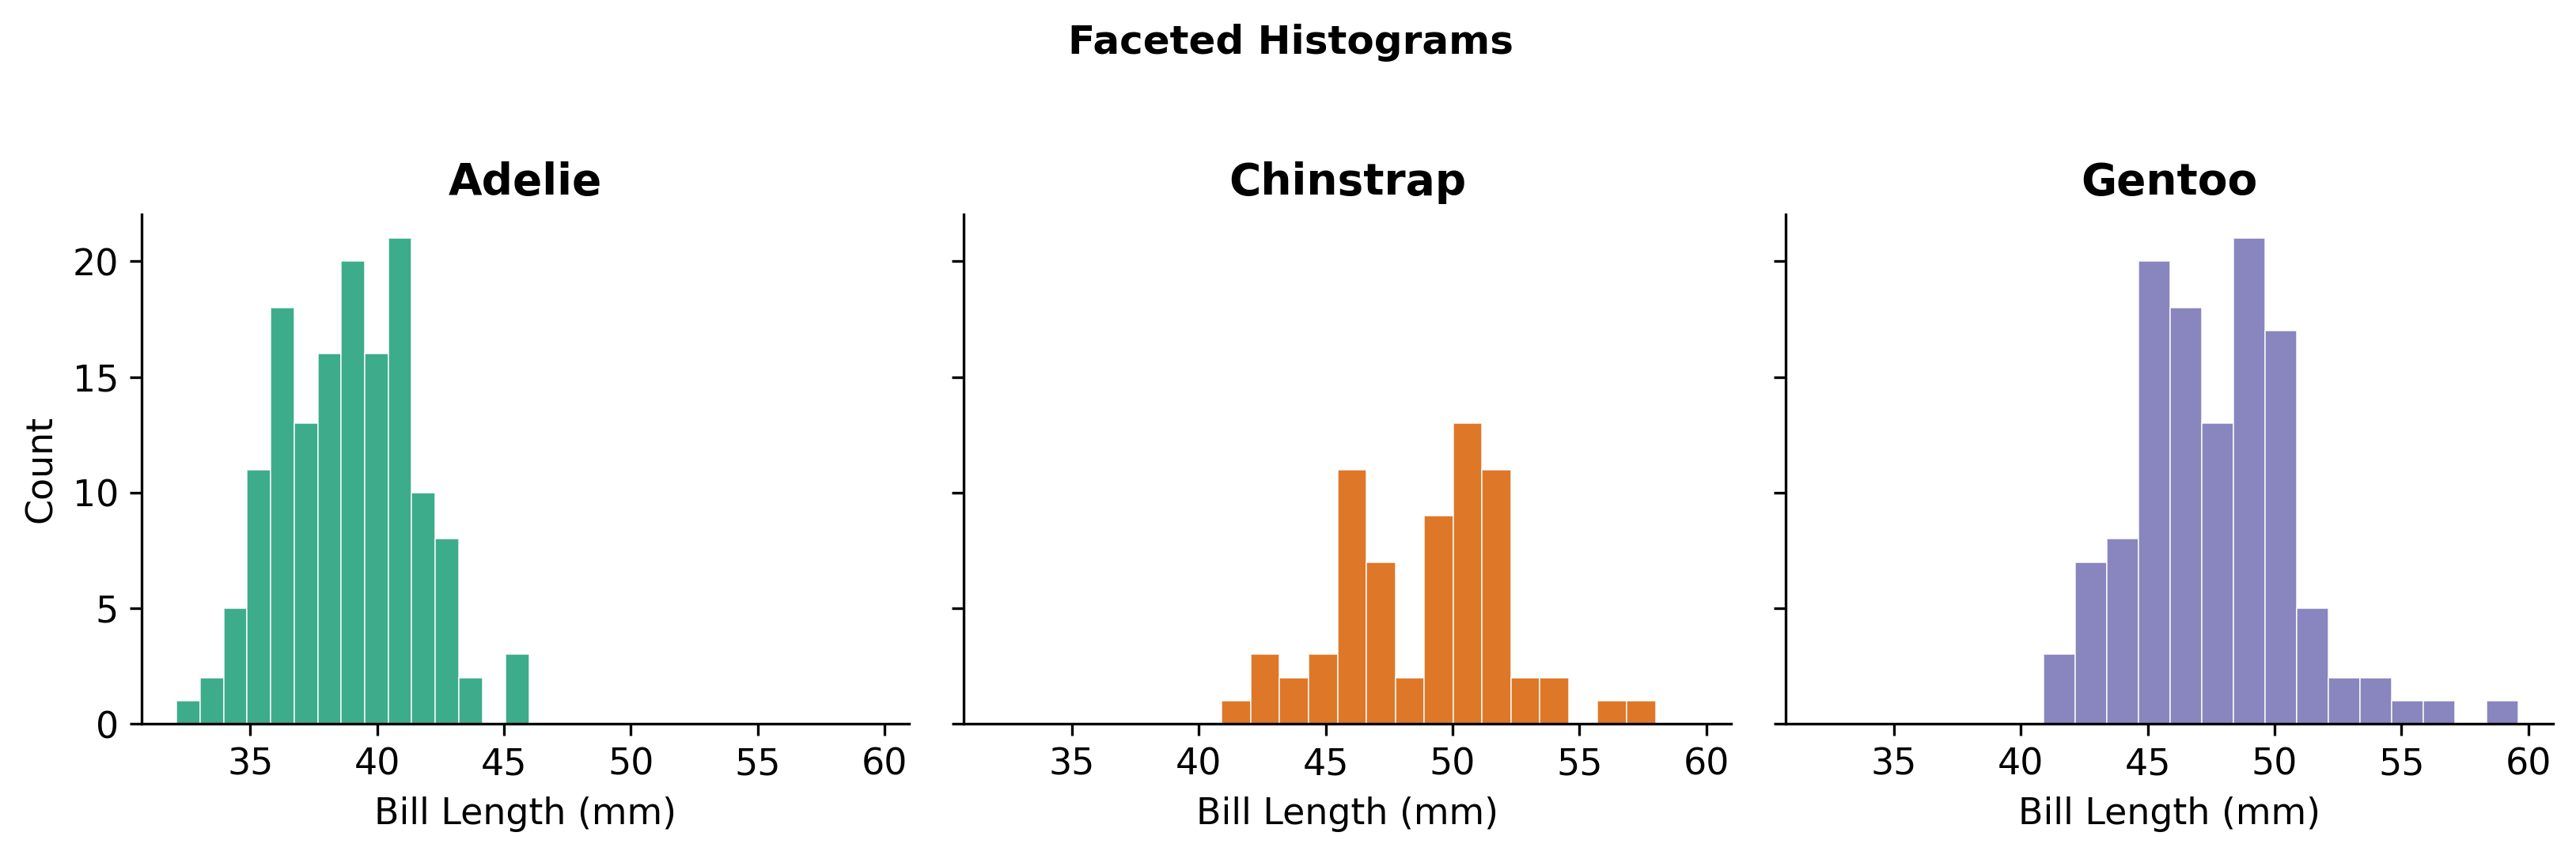
\includegraphics[width=\textwidth]{m1_4_faceted_hist.png}
\begin{exampleblock}{Data Insight}
    \scriptsize Each species' shape is unobstructed. Shared $x$-axis makes location comparison easy. Shared $y$-axis makes height comparison valid.
\end{exampleblock}
\end{column}
\end{columns}
\end{frame}

% ── 117 ──
\begin{frame}[fragile]{Faceted Histogram --- \Rlang}\smark{117/300}
\begin{columns}[T]
\begin{column}{0.55\textwidth}
\begin{lstlisting}[style=Rstyle]
ggplot(penguins,
  aes(bill_length_mm,
      fill = species)) +
  geom_histogram(bins = 15,
    color = "white",
    show.legend = FALSE) +
  facet_wrap(~species, ncol = 3) +
  scale_fill_manual(
    values=c("#1B9E77","#D95F02",
             "#7570B3")) +
  theme_minimal()
\end{lstlisting}
\end{column}
\begin{column}{0.42\textwidth}
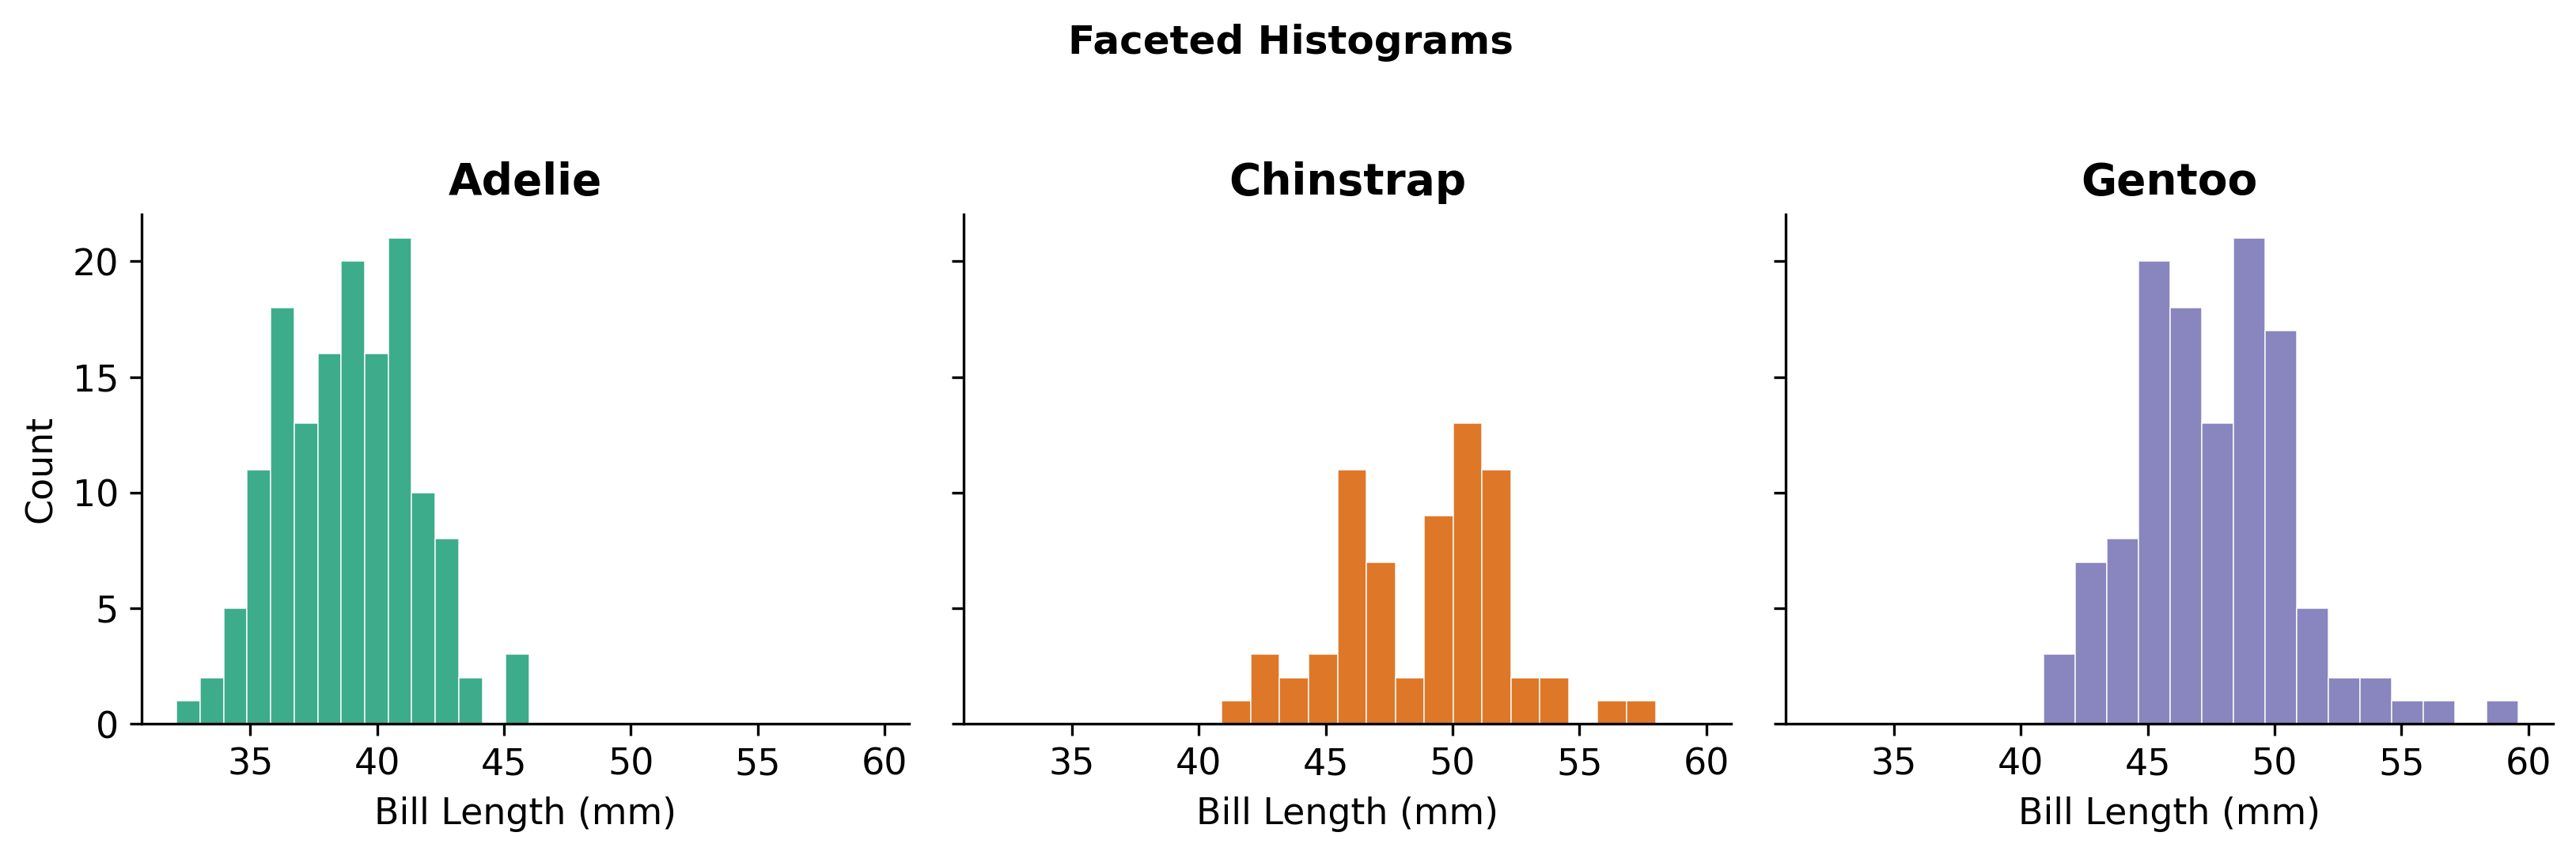
\includegraphics[width=\textwidth]{m1_4_faceted_hist.png}
\begin{alertblock}{Pro-Tip}
    \scriptsize Add \texttt{scales="free\_y"} to \texttt{facet\_wrap()} if group sizes differ dramatically and you want to see shape, not count.
\end{alertblock}
\end{column}
\end{columns}
\end{frame}

% ── 118 ──
\begin{frame}[fragile]{Faceted Histogram --- \Python}\smark{118/300}
\begin{columns}[T]
\begin{column}{0.55\textwidth}
\begin{lstlisting}[style=Pystyle]
# plotnine
(ggplot(penguins,
   aes("bill_length_mm",
       fill="species"))
 + geom_histogram(bins=15,
     color="white")
 + facet_wrap("~species", ncol=3)
 + theme_minimal()
 + theme(legend_position="none"))

# seaborn FacetGrid
g = sns.FacetGrid(penguins,
    col="species", height=3)
g.map(plt.hist, "bill_length_mm",
      bins=15, color="#B2182B",
      edgecolor="white")
\end{lstlisting}
\end{column}
\begin{column}{0.42\textwidth}
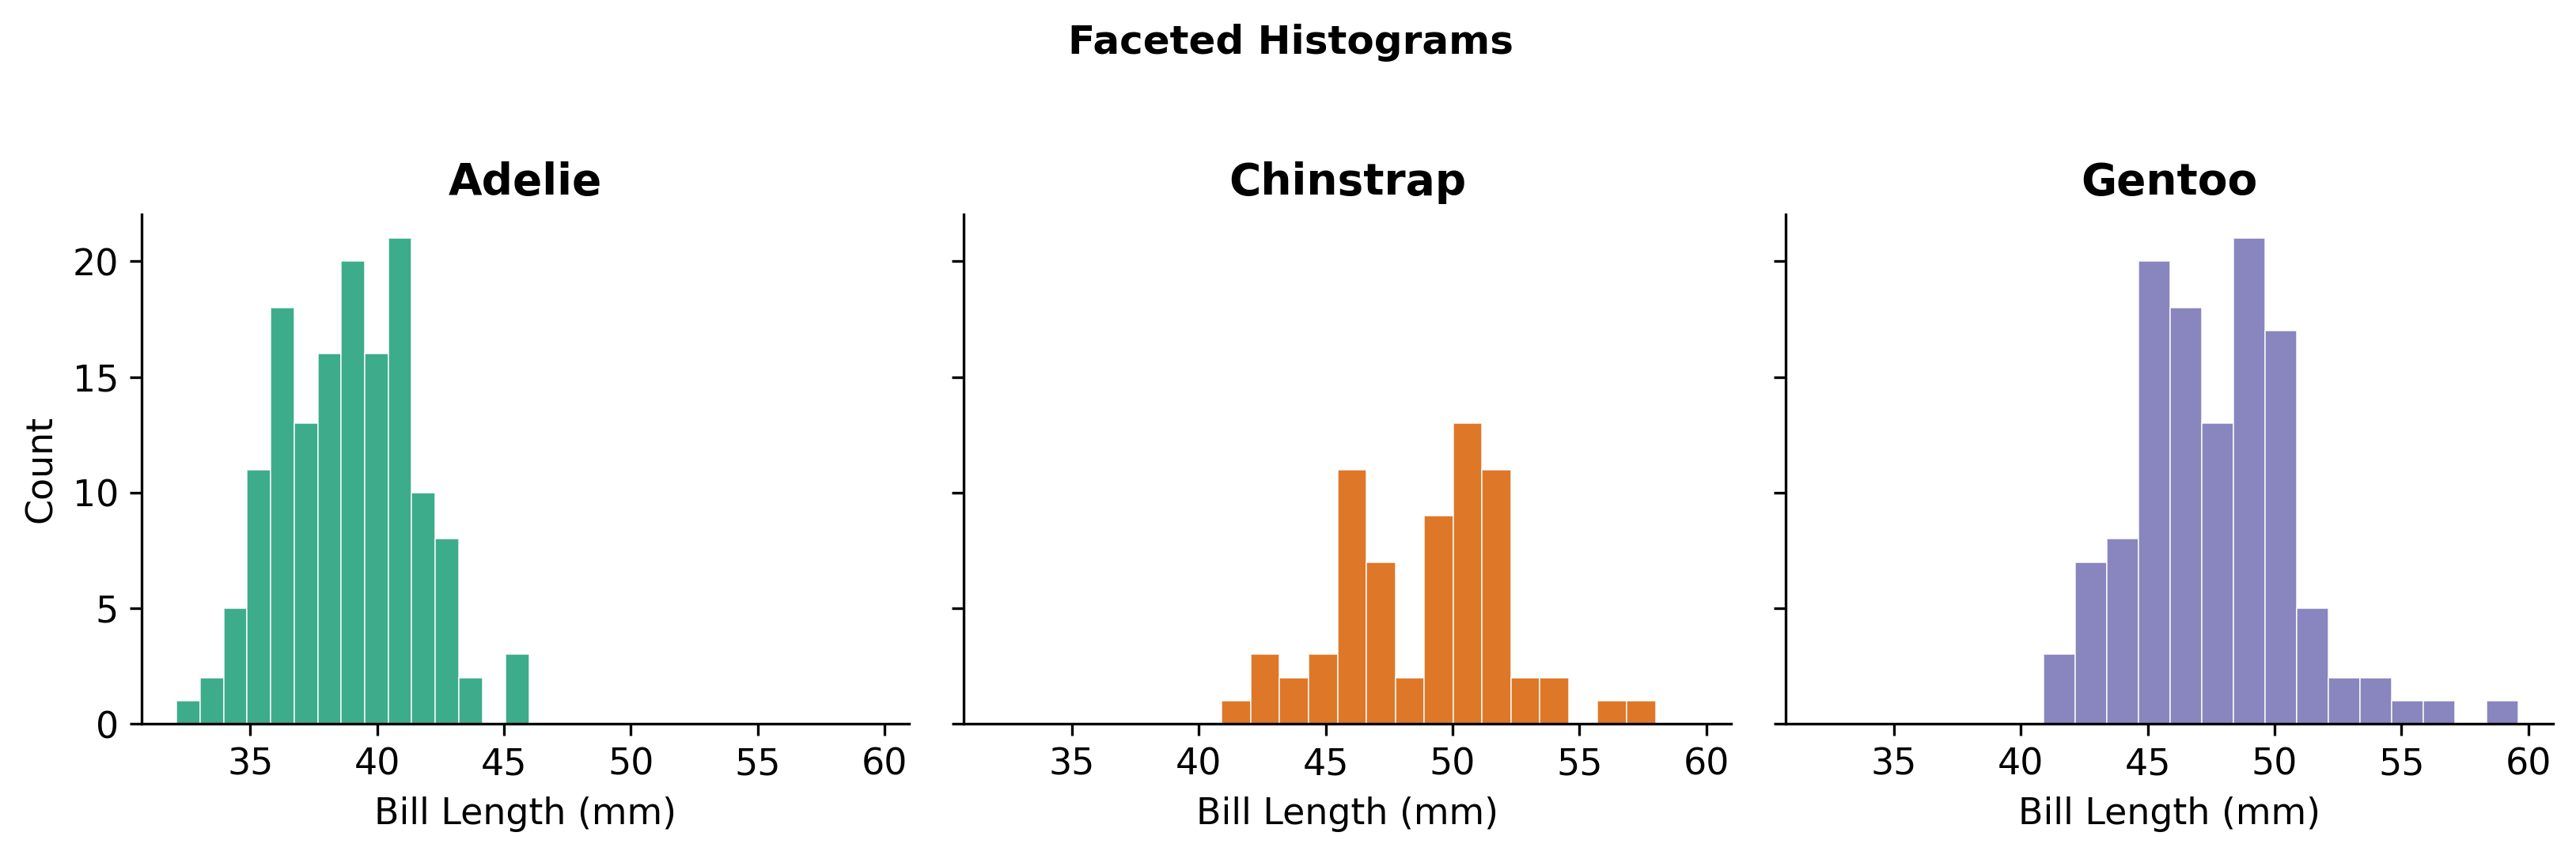
\includegraphics[width=\textwidth]{m1_4_faceted_hist.png}
\begin{exampleblock}{Data Insight}
    \scriptsize \texttt{FacetGrid.map()} in seaborn applies any matplotlib function across panels. Powerful but more verbose than plotnine.
\end{exampleblock}
\end{column}
\end{columns}
\end{frame}

% ── 119 ──
\begin{frame}{Module 1.4 --- Key Takeaways}\smark{119/300}
\begin{enumerate}
    \item \textbf{Always set binwidth explicitly.} Defaults are arbitrary.
    \item \textbf{Binwidth $\neq$ bandwidth.} Bins are for histograms; bandwidth is for KDE.
    \item \textbf{Overlay hist + KDE + rug} for the richest single-variable view.
    \item \textbf{Grouped histograms fail at 3+ groups.} Switch to density curves or facets.
    \item \textbf{QQ plots diagnose normality} more precisely than histograms.
\end{enumerate}
\end{frame}

% ── 120 ──
\begin{frame}{}\smark{120/300}
\centering\vspace{1.5cm}
{\Large\textbf{Module 1.4 Complete}}\\[0.5cm]
You can now visualize univariate distributions with histograms, density curves, frequency polygons, rug plots, and QQ plots --- with grouped and faceted variants.\\[0.5cm]
\textbf{Next:} Module 1.5 --- Aesthetic Mapping: Color, Shape, Size, Alpha.
\end{frame}

% ═══════════════════════════════════════════════════════
%  MODULE 1.5 — Aesthetic Mapping: Color, Shape, Size, Alpha
% ═══════════════════════════════════════════════════════
\section{Module 1.5 --- Aesthetic Mapping: Color, Shape, Size, Alpha}

% ── 121 ──
\begin{frame}{Module 1.5 --- Roadmap}\smark{121/300}
\begin{enumerate}
    \item Continuous vs.\ discrete color scales
    \item Sequential, diverging, and qualitative palettes
    \item Shape encoding and its limits
    \item Size encoding for a continuous third variable
    \item Alpha transparency as a density channel
    \item Combining multiple aesthetics
    \item When color fails: the colorblind problem
    \item The ``highlight one, grey the rest'' pattern
\end{enumerate}
\end{frame}

% ── 122 ──
\begin{frame}{Why Aesthetics Are the Grammar's Power Tool}
\smark{122/300}
\begin{columns}[T]
\begin{column}{0.50\textwidth}
\begin{itemize}
    \item Position ($x$, $y$) encodes 2 variables
    \item Color, size, shape, alpha encode \textbf{3rd, 4th, 5th} variables without adding panels
    \item Choice of aesthetic determines what the viewer \textbf{sees first}
    \item Mismatched aesthetic $\to$ misread data
\end{itemize}
\end{column}
\begin{column}{0.47\textwidth}
\begin{exampleblock}{Data Insight}
    \scriptsize Mackinlay (1986): for \textbf{quantitative} data, use position $>$ length $>$ color value $>$ size. For \textbf{categorical} data, use position $>$ color hue $>$ shape.
\end{exampleblock}
\vspace{0.2cm}
\begin{alertblock}{Pro-Tip}
    \scriptsize Never map a continuous variable to shape. Shape has no natural ordering.
\end{alertblock}
\end{column}
\end{columns}
\end{frame}

% ── 123 ──
\begin{frame}{Color Scales: Continuous vs.\ Discrete}
\smark{123/300}
\centering\small
\begin{tabular}{@{}lll@{}}
    \toprule
    \textbf{Variable Type} & \textbf{Scale Type} & \textbf{ggplot2 Example} \\
    \midrule
    Continuous (e.g., mass)    & Gradient   & \texttt{scale\_color\_viridis\_c()} \\
    Discrete (e.g., species)   & Qualitative & \texttt{scale\_color\_brewer(palette="Dark2")} \\
    Ordered factor             & Sequential  & \texttt{scale\_color\_brewer(palette="Blues")} \\
    Diverging (e.g., anomaly)  & Diverging   & \texttt{scale\_color\_gradient2()} \\
    \bottomrule
\end{tabular}

\vspace{0.3cm}
\begin{exampleblock}{Data Insight}
    \scriptsize Mapping a continuous variable to a qualitative palette (e.g., ``Set2'') is a \textbf{type mismatch} --- there is no perceptual ordering in qualitative hues. The viewer cannot tell which value is larger.
\end{exampleblock}
\end{frame}

% ── 124 ──
\begin{frame}{Sequential Palettes}
\smark{124/300}
\centering
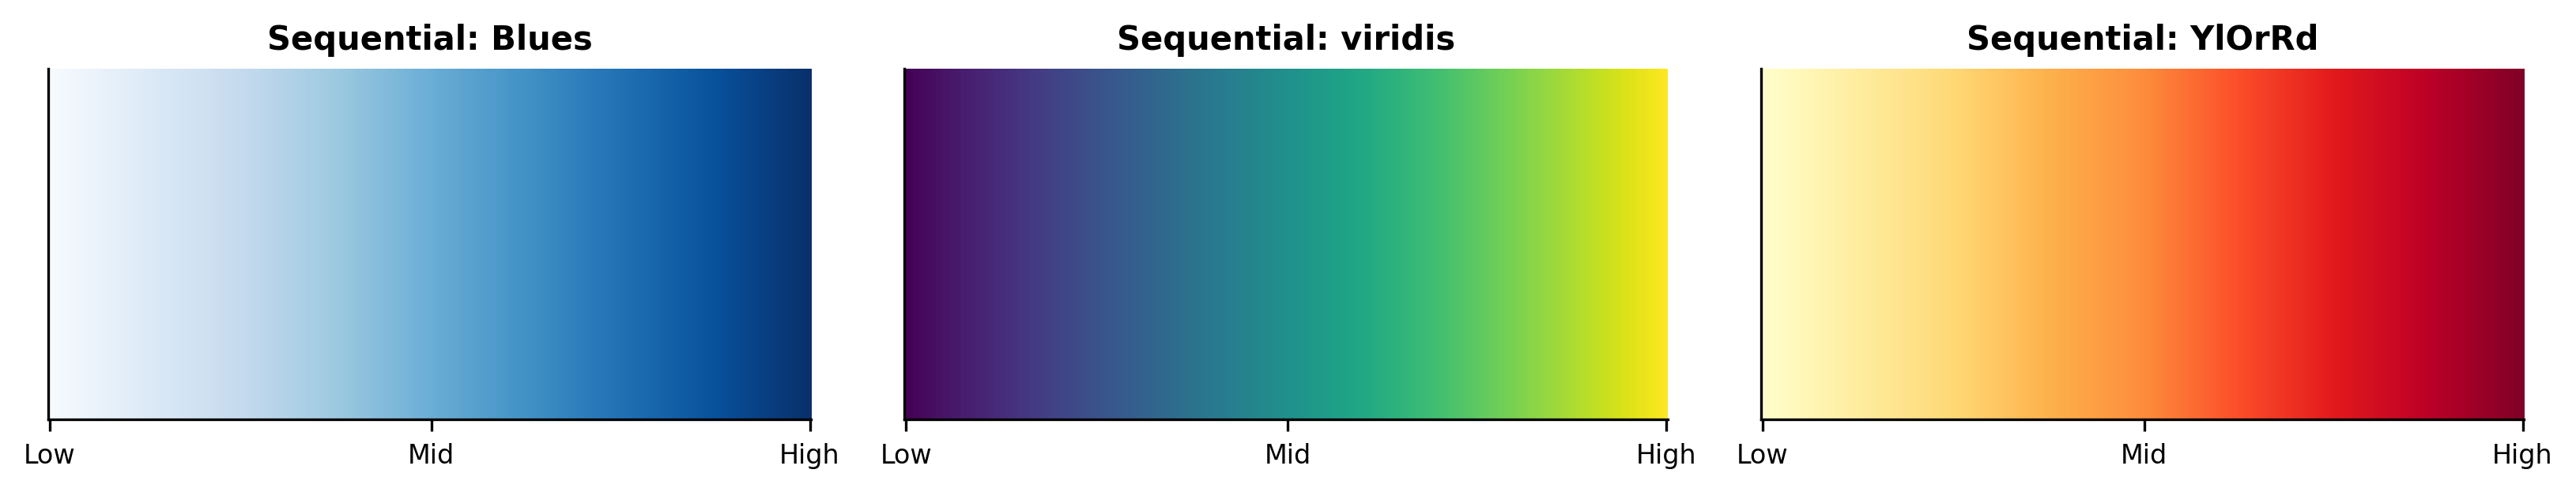
\includegraphics[width=0.92\textwidth]{m1_5_sequential.png}

\vspace{0.3cm}
\begin{columns}[T]
\begin{column}{0.48\textwidth}
\begin{itemize}
    \item Light $\to$ dark encodes low $\to$ high
    \item Best for \textbf{magnitudes}: counts, temperatures, concentrations
    \item \texttt{viridis} is perceptually uniform \textbf{and} colorblind-safe
\end{itemize}
\end{column}
\begin{column}{0.48\textwidth}
\begin{alertblock}{Pro-Tip}
    \scriptsize Avoid rainbow/jet: it is not perceptually uniform, has false boundaries, and fails for colorblind viewers (Borland \& Taylor, 2007).
\end{alertblock}
\end{column}
\end{columns}
\end{frame}

% ── 125 ──
\begin{frame}{Diverging Palettes}
\smark{125/300}
\centering
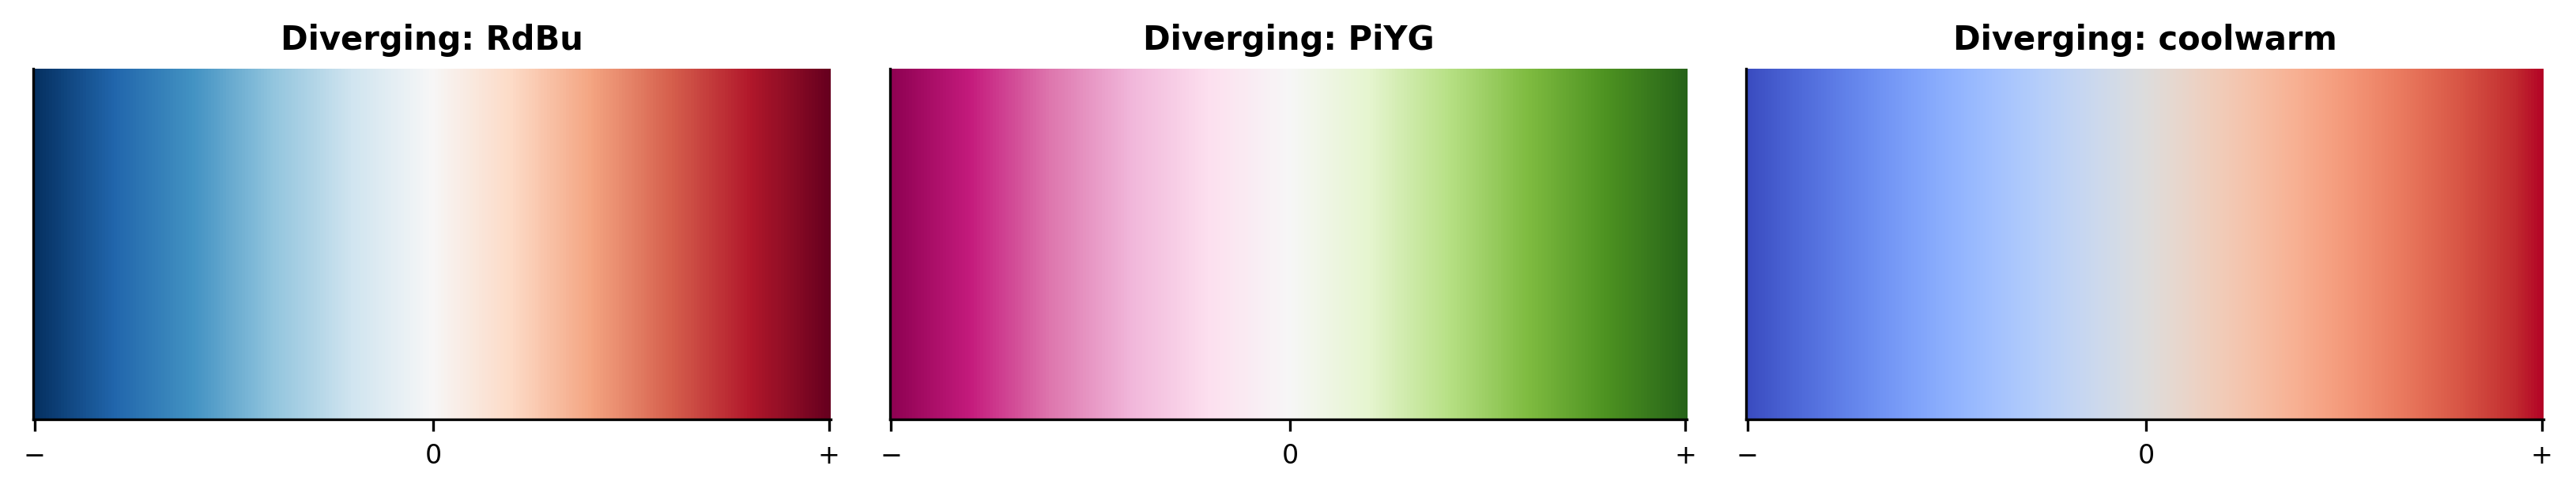
\includegraphics[width=0.92\textwidth]{m1_5_diverging.png}

\vspace{0.3cm}
\begin{columns}[T]
\begin{column}{0.48\textwidth}
\begin{itemize}
    \item Two hues diverge from a neutral midpoint
    \item Best when a \textbf{meaningful center} exists: zero, mean, threshold
    \item E.g., temperature anomaly, correlation, profit/loss
\end{itemize}
\end{column}
\begin{column}{0.48\textwidth}
\begin{exampleblock}{Data Insight}
    \scriptsize The midpoint must be \textbf{meaningful}. If your data ranges 50--100, a diverging palette centered at 75 implies 75 is ``neutral'' --- is it?
\end{exampleblock}
\end{column}
\end{columns}
\end{frame}

% ── 126 ──
\begin{frame}{Qualitative Palettes}
\smark{126/300}
\centering
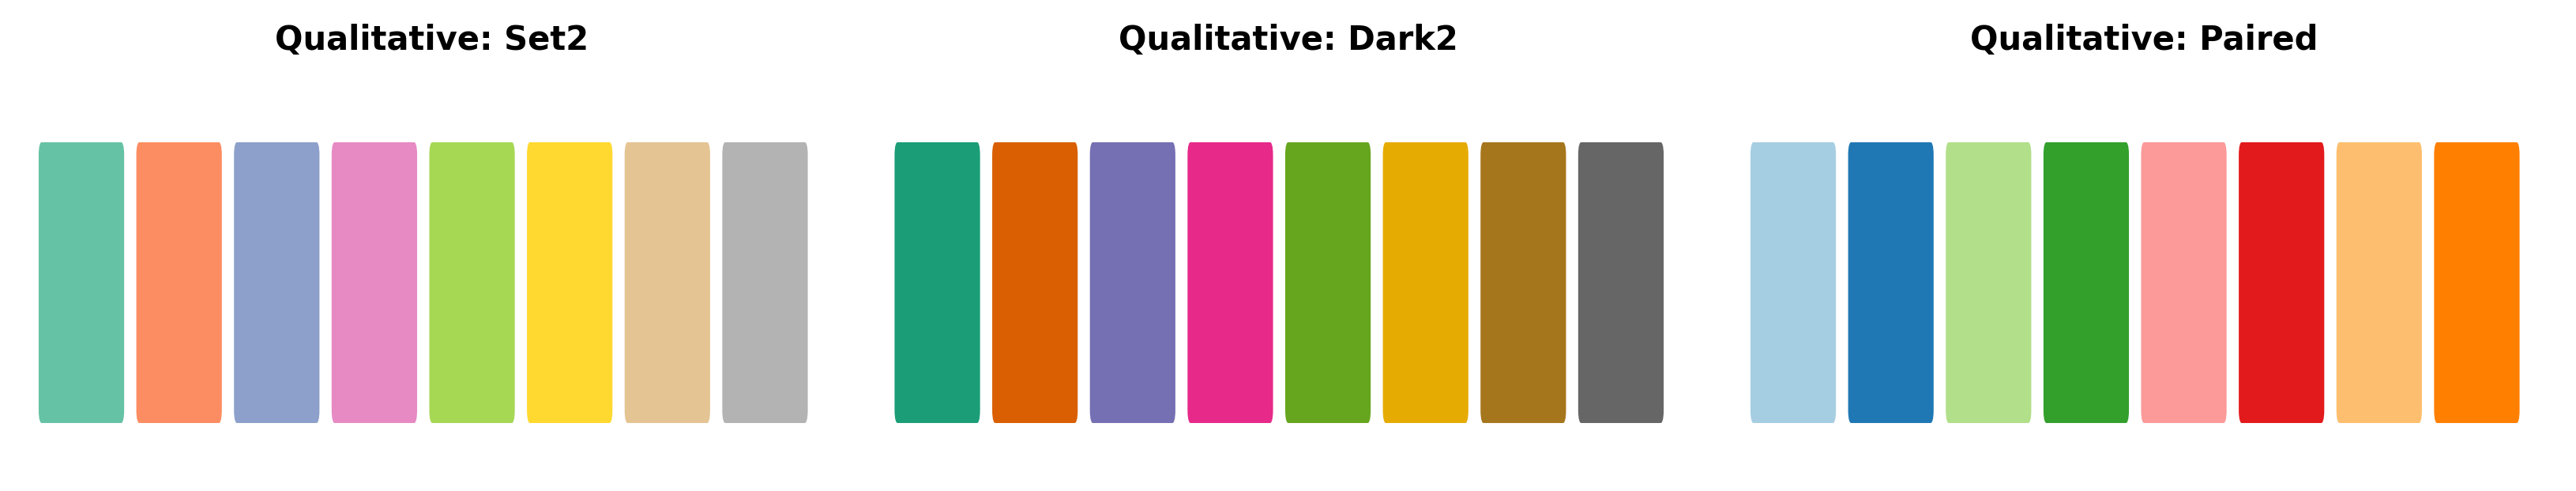
\includegraphics[width=0.92\textwidth]{m1_5_qualitative.png}

\vspace{0.3cm}
\begin{columns}[T]
\begin{column}{0.48\textwidth}
\begin{itemize}
    \item Maximally distinct hues, no inherent order
    \item Best for \textbf{nominal} categories: species, country, group
    \item Practical limit: \textbf{6--8 colors} before confusion
\end{itemize}
\end{column}
\begin{column}{0.48\textwidth}
\begin{alertblock}{Pro-Tip}
    \scriptsize If you have $>$8 categories, consider faceting or the ``highlight one, grey rest'' pattern (slide 148) instead of adding more colors.
\end{alertblock}
\end{column}
\end{columns}
\end{frame}

% ── 127 ──
\begin{frame}[fragile]{Continuous Color --- \Rlang}\smark{127/300}
\begin{columns}[T]
\begin{column}{0.55\textwidth}
\begin{lstlisting}[style=Rstyle]
ggplot(penguins,
  aes(x = bill_length_mm,
      y = flipper_length_mm,
      color = body_mass_g)) +
  geom_point(size = 2.5,
             alpha = 0.8) +
  scale_color_viridis_c() +
  labs(color = "Mass (g)") +
  theme_minimal()
\end{lstlisting}
\end{column}
\begin{column}{0.42\textwidth}
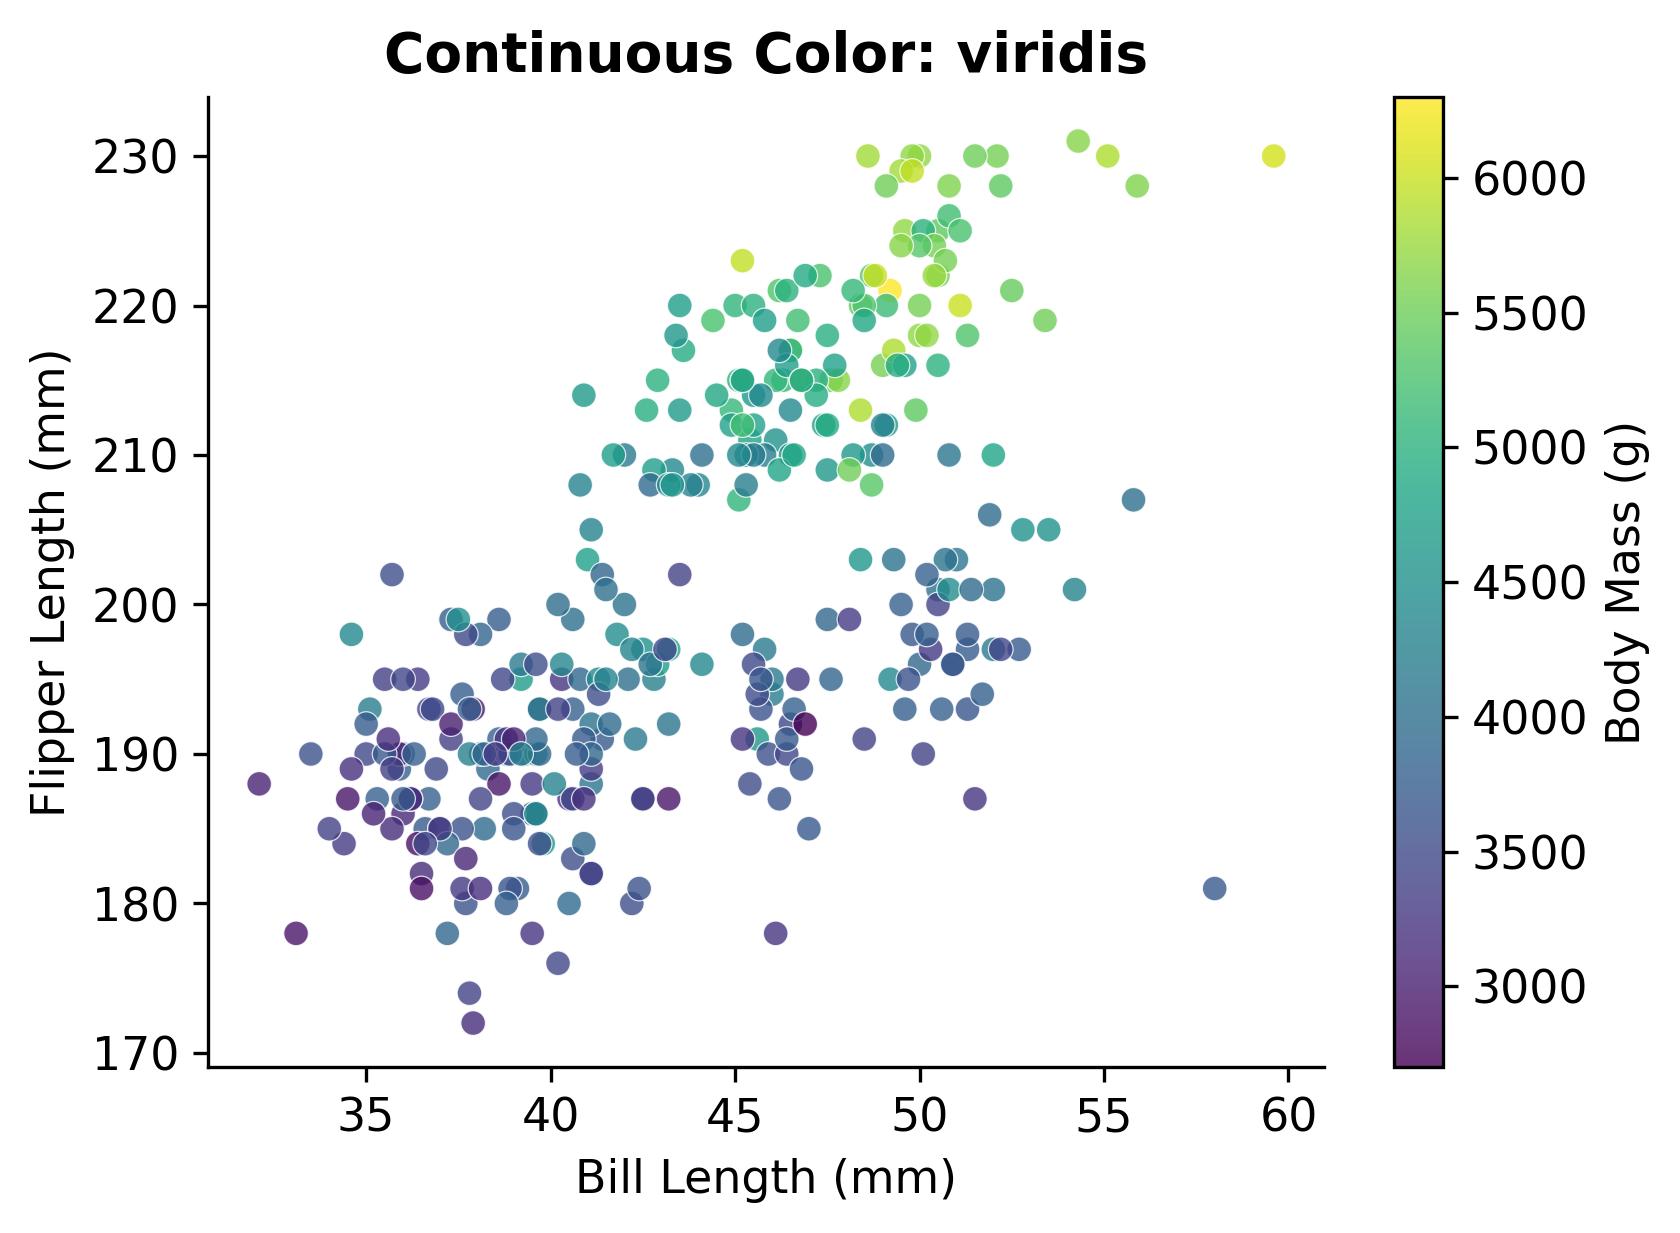
\includegraphics[width=\textwidth]{m1_5_color_continuous.png}
\begin{exampleblock}{Data Insight}
    \scriptsize Heavier penguins (yellow) cluster at high bill + flipper length. The gradient makes magnitude comparison instant.
\end{exampleblock}
\end{column}
\end{columns}
\end{frame}

% ── 128 ──
\begin{frame}[fragile]{Continuous Color --- \Python}\smark{128/300}
\begin{columns}[T]
\begin{column}{0.55\textwidth}
\begin{lstlisting}[style=Pystyle]
# plotnine
(ggplot(penguins,
   aes("bill_length_mm",
       "flipper_length_mm",
       color="body_mass_g"))
 + geom_point(size=2.5, alpha=0.8)
 + scale_color_cmap("viridis")
 + labs(color="Mass (g)"))

# matplotlib
sc = ax.scatter(x, y, c=mass,
    cmap="viridis", s=30)
plt.colorbar(sc, label="Mass (g)")
\end{lstlisting}
\end{column}
\begin{column}{0.42\textwidth}
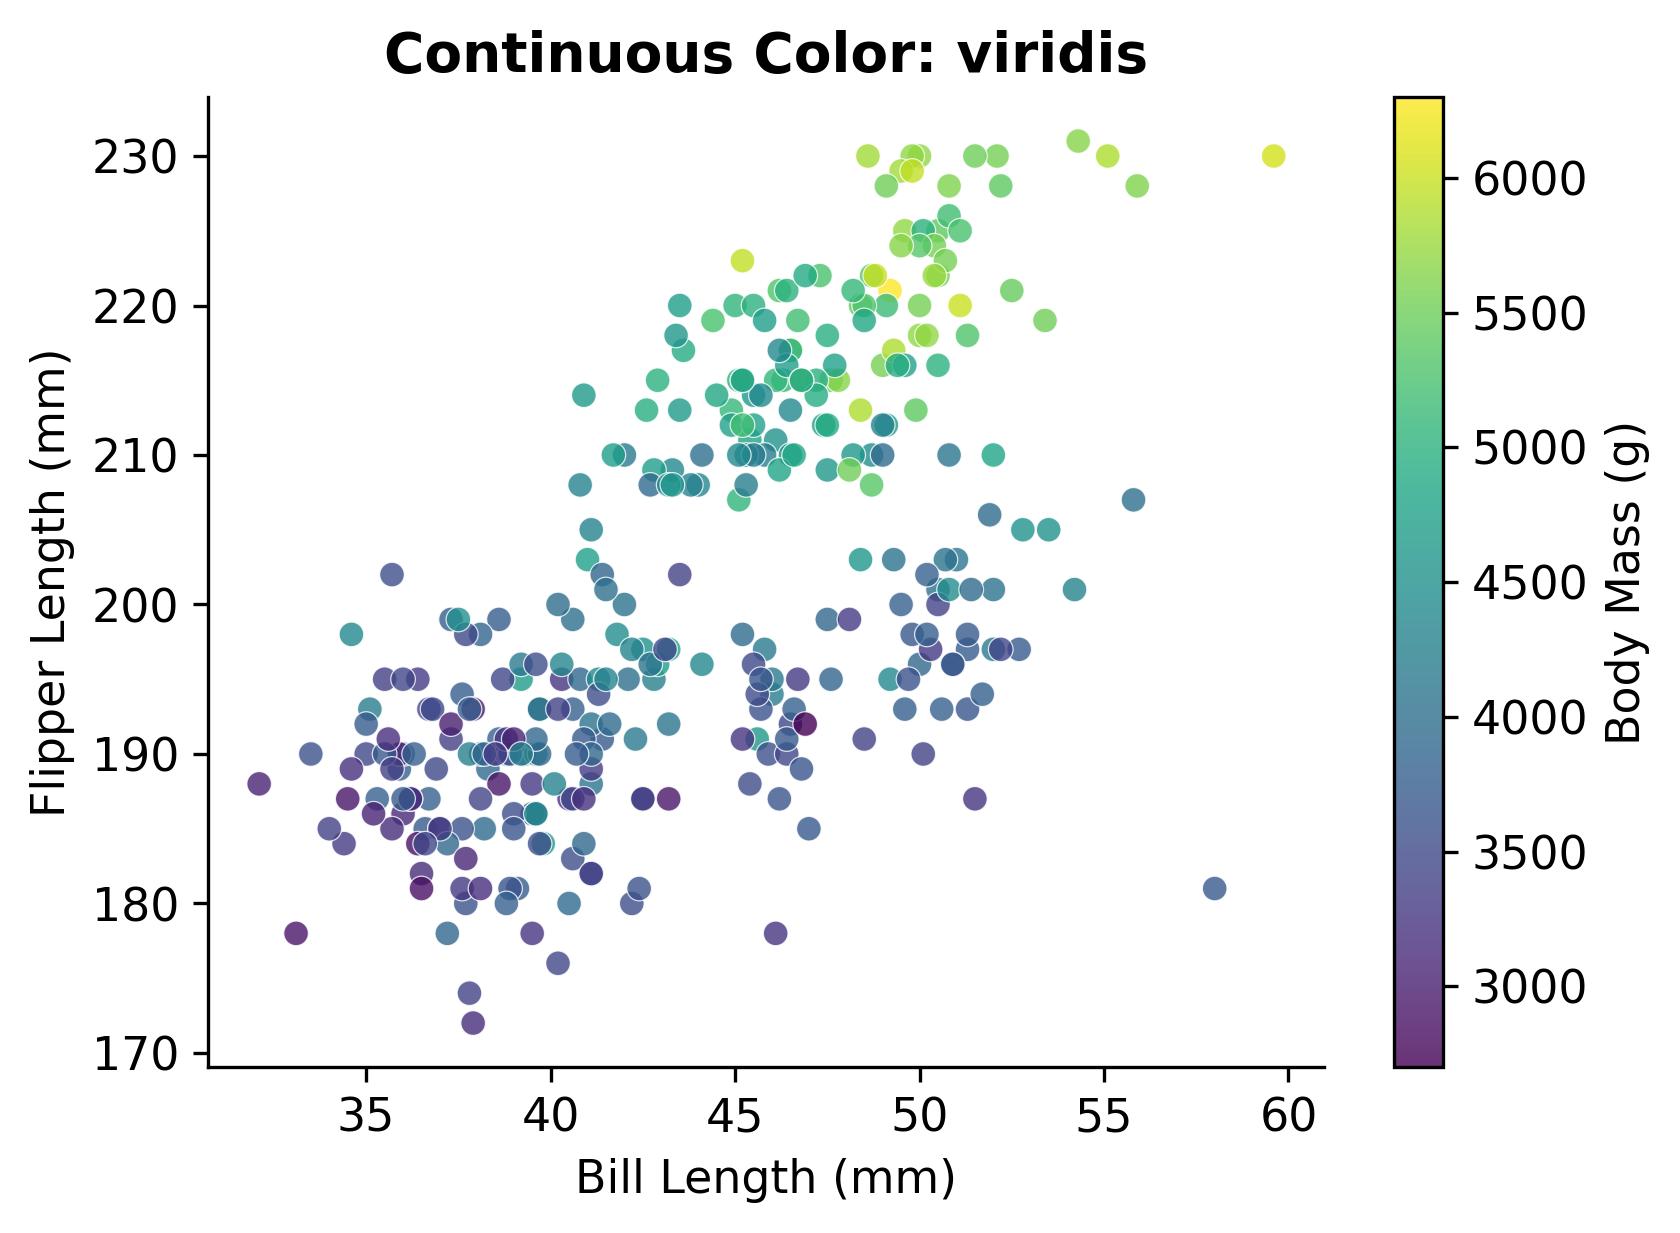
\includegraphics[width=\textwidth]{m1_5_color_continuous.png}
\begin{alertblock}{Pro-Tip}
    \scriptsize In plotnine: \texttt{scale\_color\_cmap()}. In matplotlib: the \texttt{c=} and \texttt{cmap=} arguments to \texttt{scatter()}.
\end{alertblock}
\end{column}
\end{columns}
\end{frame}

% ── 129 ──
\begin{frame}[fragile]{Discrete Color --- \Rlang}\smark{129/300}
\begin{columns}[T]
\begin{column}{0.55\textwidth}
\begin{lstlisting}[style=Rstyle]
ggplot(penguins,
  aes(bill_length_mm,
      flipper_length_mm,
      color = species)) +
  geom_point(alpha = 0.8) +
  scale_color_manual(
    values = c("#1B9E77",
               "#D95F02",
               "#7570B3")) +
  theme_minimal()
\end{lstlisting}
\end{column}
\begin{column}{0.42\textwidth}
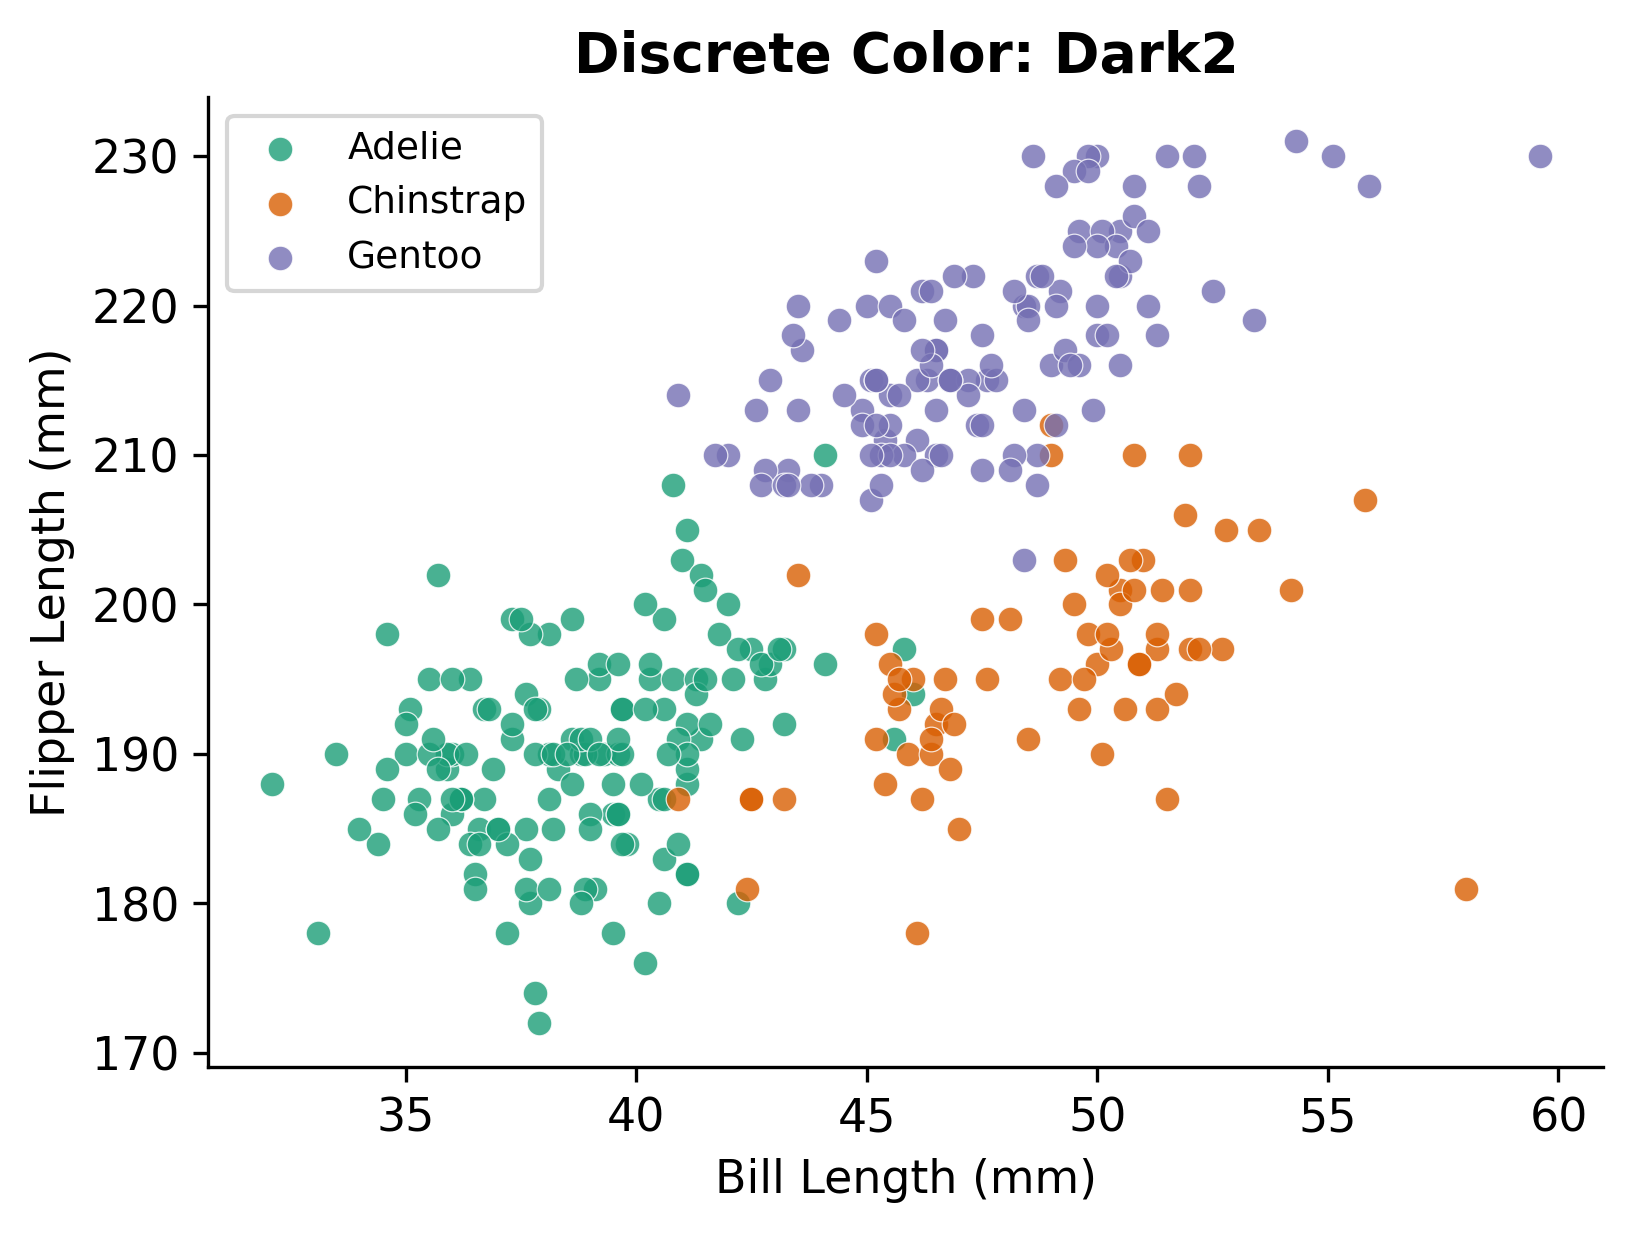
\includegraphics[width=\textwidth]{m1_5_color_discrete.png}
\begin{alertblock}{Pro-Tip}
    \scriptsize \texttt{scale\_color\_manual()} for exact control. \texttt{scale\_color\_brewer()} for pre-built palettes. Never use both on the same aesthetic.
\end{alertblock}
\end{column}
\end{columns}
\end{frame}

% ── 130 ──
\begin{frame}[fragile]{Discrete Color --- \Python}\smark{130/300}
\begin{columns}[T]
\begin{column}{0.55\textwidth}
\begin{lstlisting}[style=Pystyle]
# plotnine
(ggplot(penguins,
   aes("bill_length_mm",
       "flipper_length_mm",
       color="species"))
 + geom_point(alpha=0.8)
 + scale_color_manual(
     values=["#1B9E77",
             "#D95F02",
             "#7570B3"]))

# seaborn: palette parameter
sns.scatterplot(data=penguins,
    x="bill_length_mm",
    y="flipper_length_mm",
    hue="species",
    palette="Dark2")
\end{lstlisting}
\end{column}
\begin{column}{0.42\textwidth}
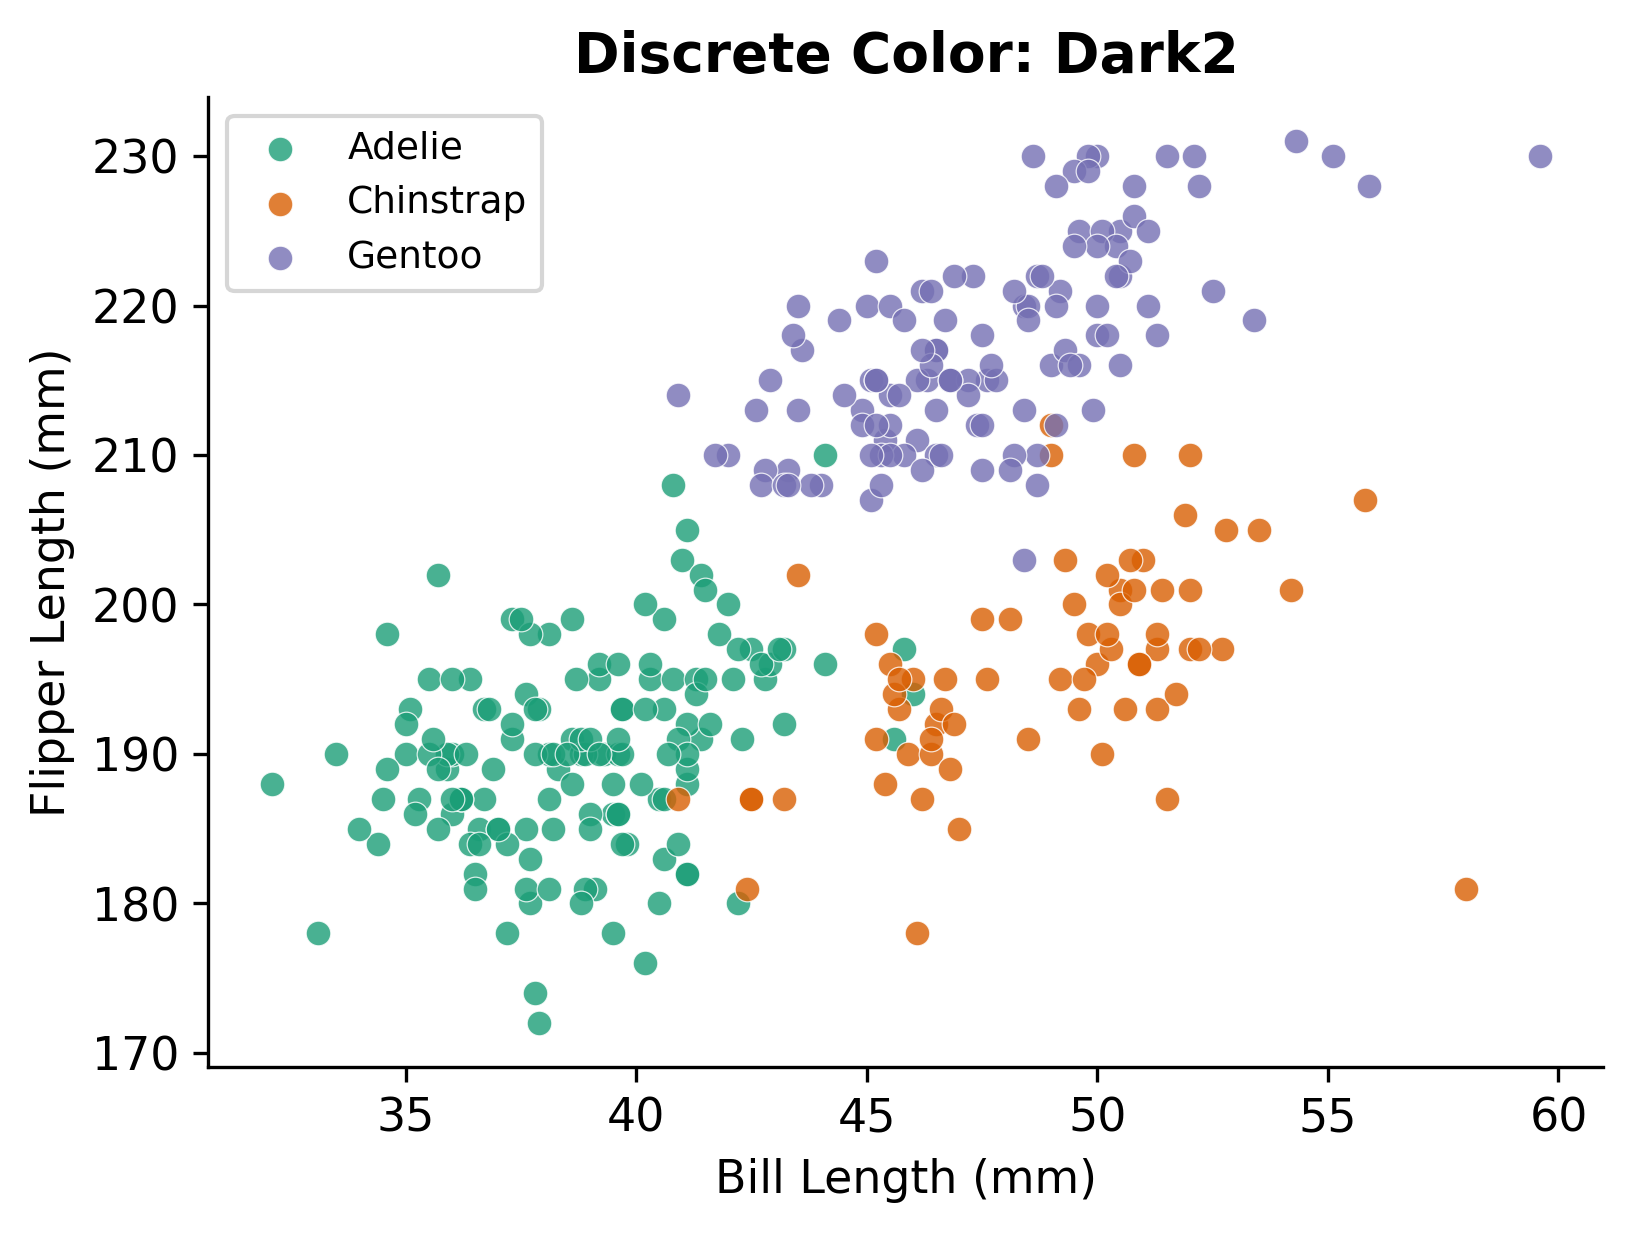
\includegraphics[width=\textwidth]{m1_5_color_discrete.png}
\end{column}
\end{columns}
\end{frame}

% ── 131 ──
\begin{frame}{Shape Encoding}
\smark{131/300}
\begin{columns}[T]
\begin{column}{0.50\textwidth}
\begin{itemize}
    \item Maps a \textbf{categorical} variable to marker shape
    \item \texttt{ggplot2} default: 6 shapes (circle, triangle, square, diamond, plus, cross)
    \item Discriminability ceiling: \textbf{$\leq$6 levels}
    \item Best used \textbf{redundantly} with color (shape + color for the same variable)
\end{itemize}
\end{column}
\begin{column}{0.47\textwidth}
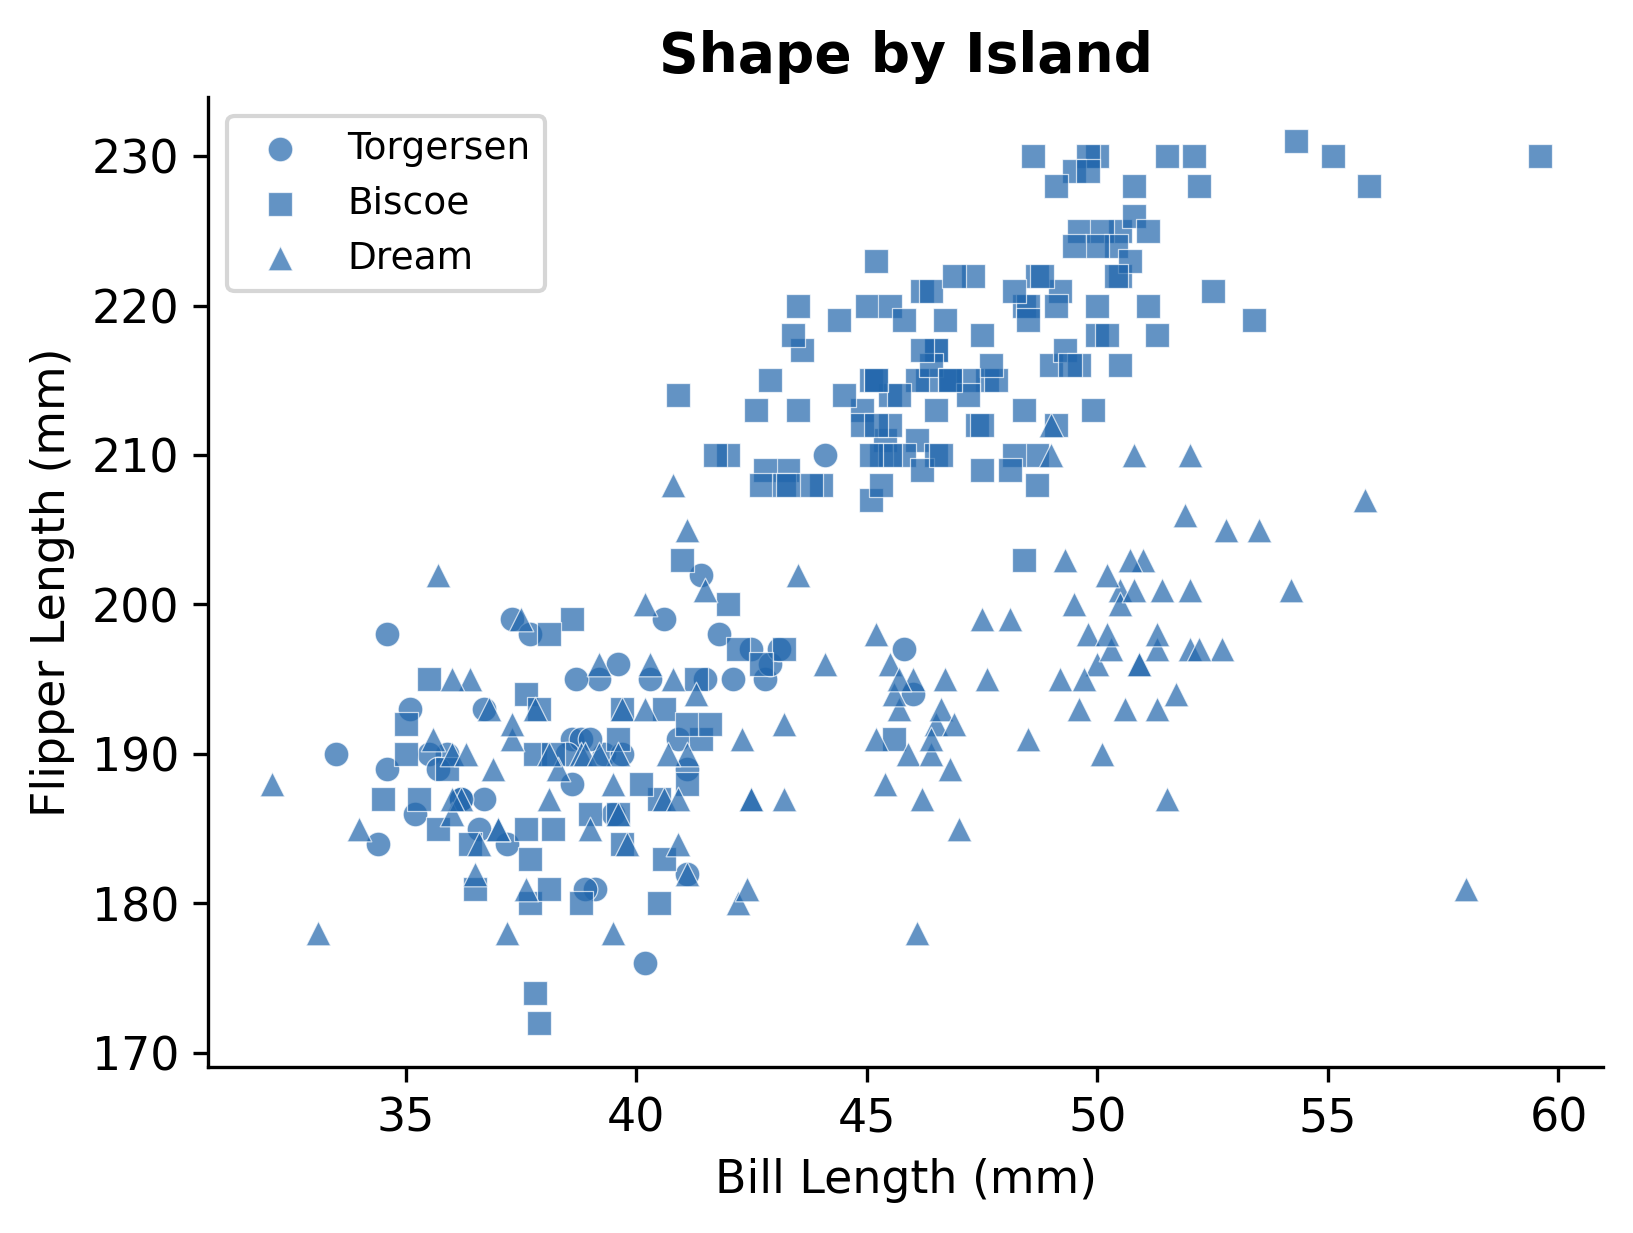
\includegraphics[width=\textwidth]{m1_5_shape.png}
\begin{exampleblock}{Data Insight}
    \scriptsize Shape alone is hard to decode at small point sizes or high density. Always pair with color when possible.
\end{exampleblock}
\end{column}
\end{columns}
\end{frame}

% ── 132 ──
\begin{frame}[fragile]{Shape --- \Rlang}\smark{132/300}
\begin{columns}[T]
\begin{column}{0.55\textwidth}
\begin{lstlisting}[style=Rstyle]
ggplot(penguins,
  aes(bill_length_mm,
      flipper_length_mm,
      shape = island)) +
  geom_point(color="#2166AC",
             size=2.5, alpha=0.7)+
  scale_shape_manual(
    values = c(16, 15, 17)) +
  theme_minimal()
# 16=circle, 15=square, 17=triangle
\end{lstlisting}
\end{column}
\begin{column}{0.42\textwidth}
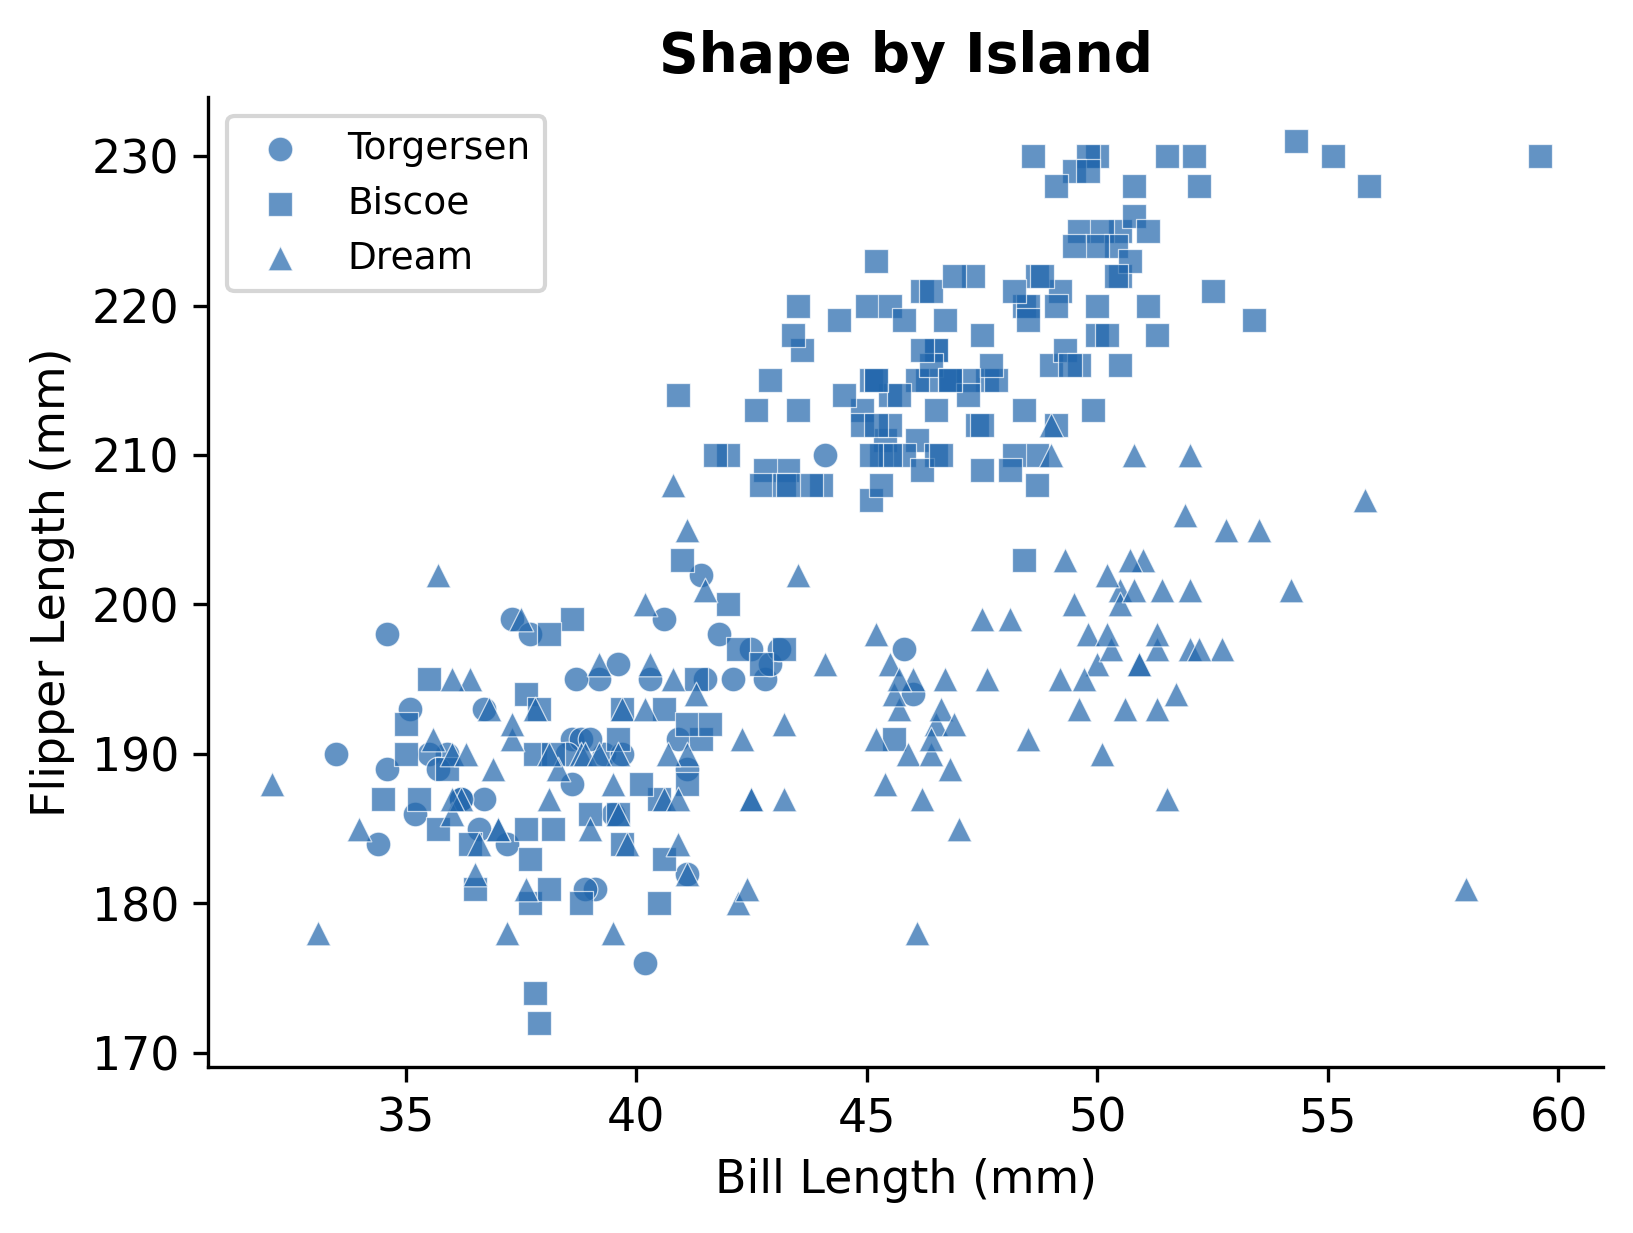
\includegraphics[width=\textwidth]{m1_5_shape.png}
\begin{alertblock}{Pro-Tip}
    \scriptsize R uses numeric shape codes (0--25). Filled shapes (15--18) are visible against any background. Open shapes (0--6) disappear at small sizes.
\end{alertblock}
\end{column}
\end{columns}
\end{frame}

% ── 133 ──
\begin{frame}[fragile]{Shape --- \Python}\smark{133/300}
\begin{columns}[T]
\begin{column}{0.55\textwidth}
\begin{lstlisting}[style=Pystyle]
# plotnine
(ggplot(penguins,
   aes("bill_length_mm",
       "flipper_length_mm",
       shape="island"))
 + geom_point(color="#B2182B",
              size=2.5, alpha=0.7))

# matplotlib: manual per-group
markers = {"Torgersen":"o",
           "Biscoe":"s",
           "Dream":"^"}
for isl, m in markers.items():
    sub = pen[pen["island"]==isl]
    ax.scatter(sub["x"], sub["y"],
               marker=m)
\end{lstlisting}
\end{column}
\begin{column}{0.42\textwidth}
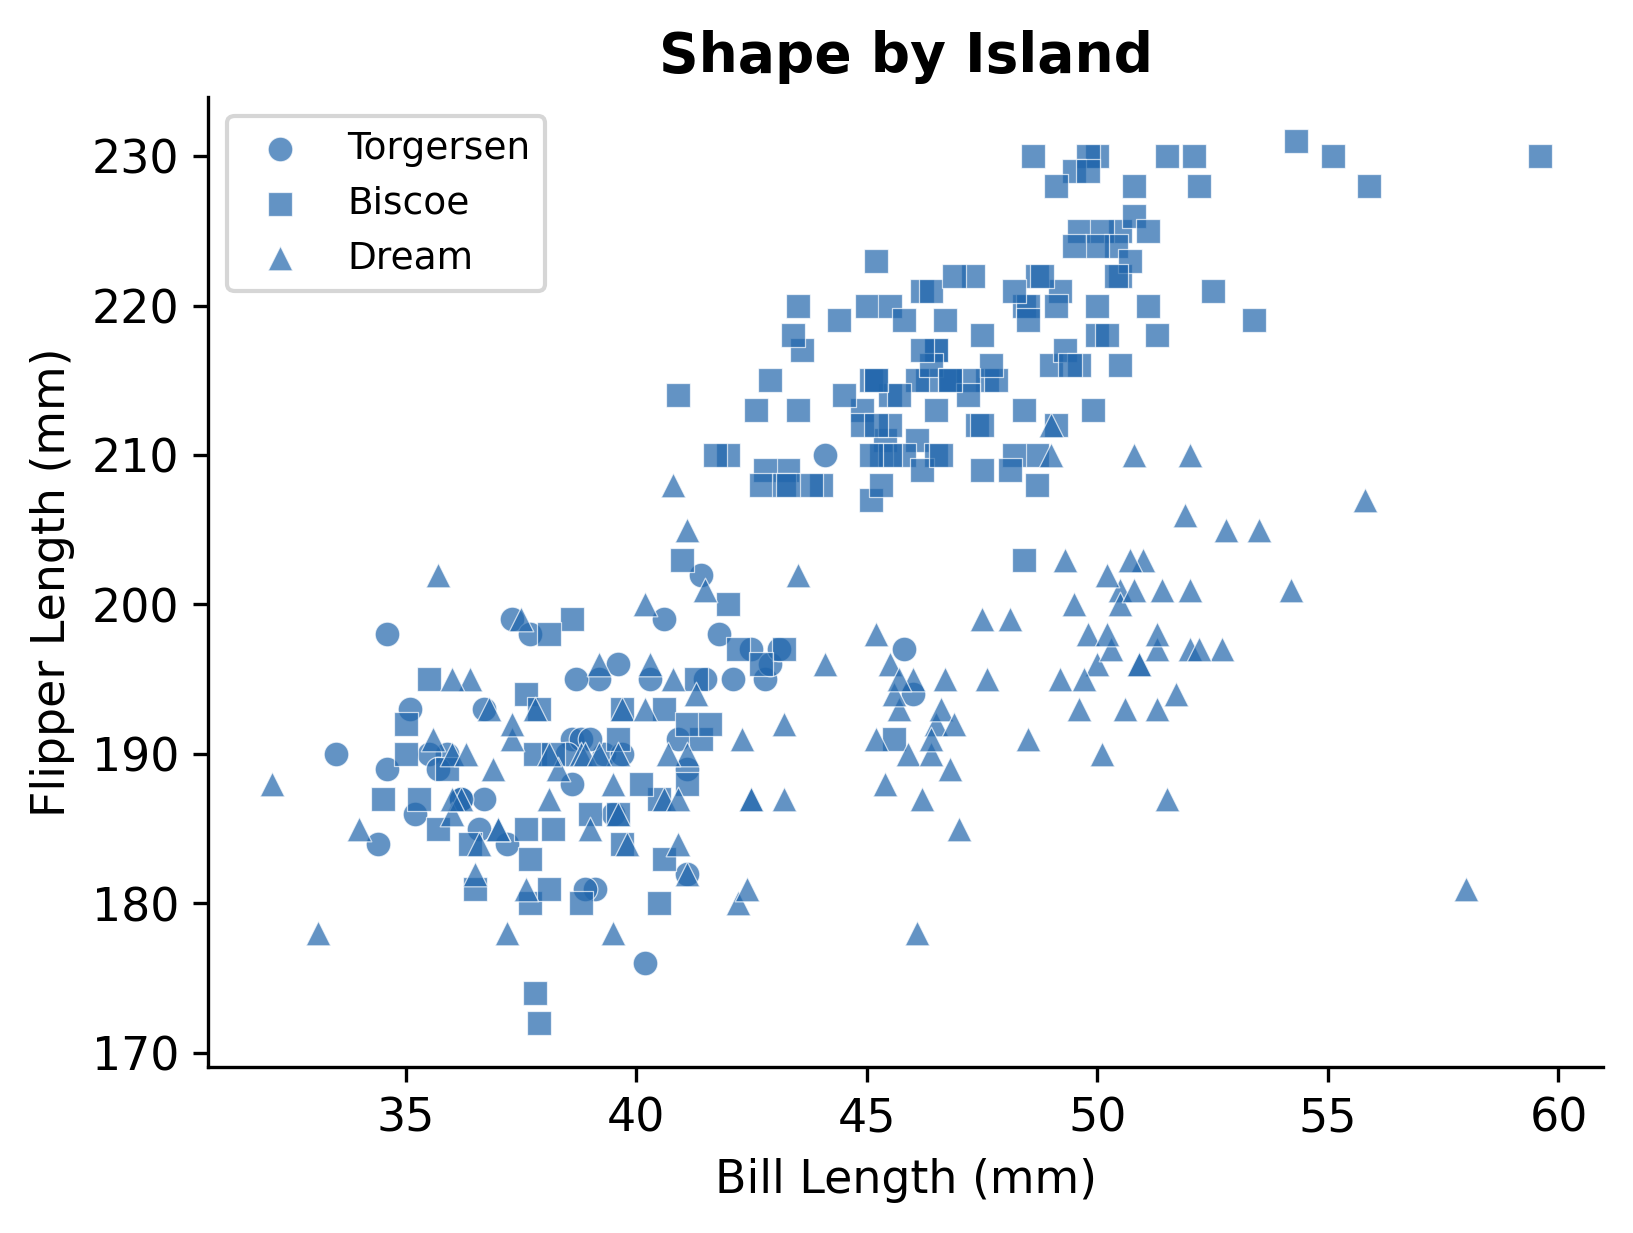
\includegraphics[width=\textwidth]{m1_5_shape.png}
\begin{exampleblock}{Data Insight}
    \scriptsize matplotlib requires a loop over groups for shape mapping. plotnine handles it declaratively.
\end{exampleblock}
\end{column}
\end{columns}
\end{frame}

% ── 134 ──
\begin{frame}{Size Encoding}
\smark{134/300}
\begin{columns}[T]
\begin{column}{0.50\textwidth}
\begin{itemize}
    \item Maps a \textbf{continuous} variable to point area
    \item Rank 5 in Cleveland--McGill hierarchy (area)
    \item Humans \textbf{underestimate} area differences (Stevens' power law, exponent $\approx 0.7$)
    \item Useful for a 3rd quantitative variable; interpret with caution
\end{itemize}
\end{column}
\begin{column}{0.47\textwidth}
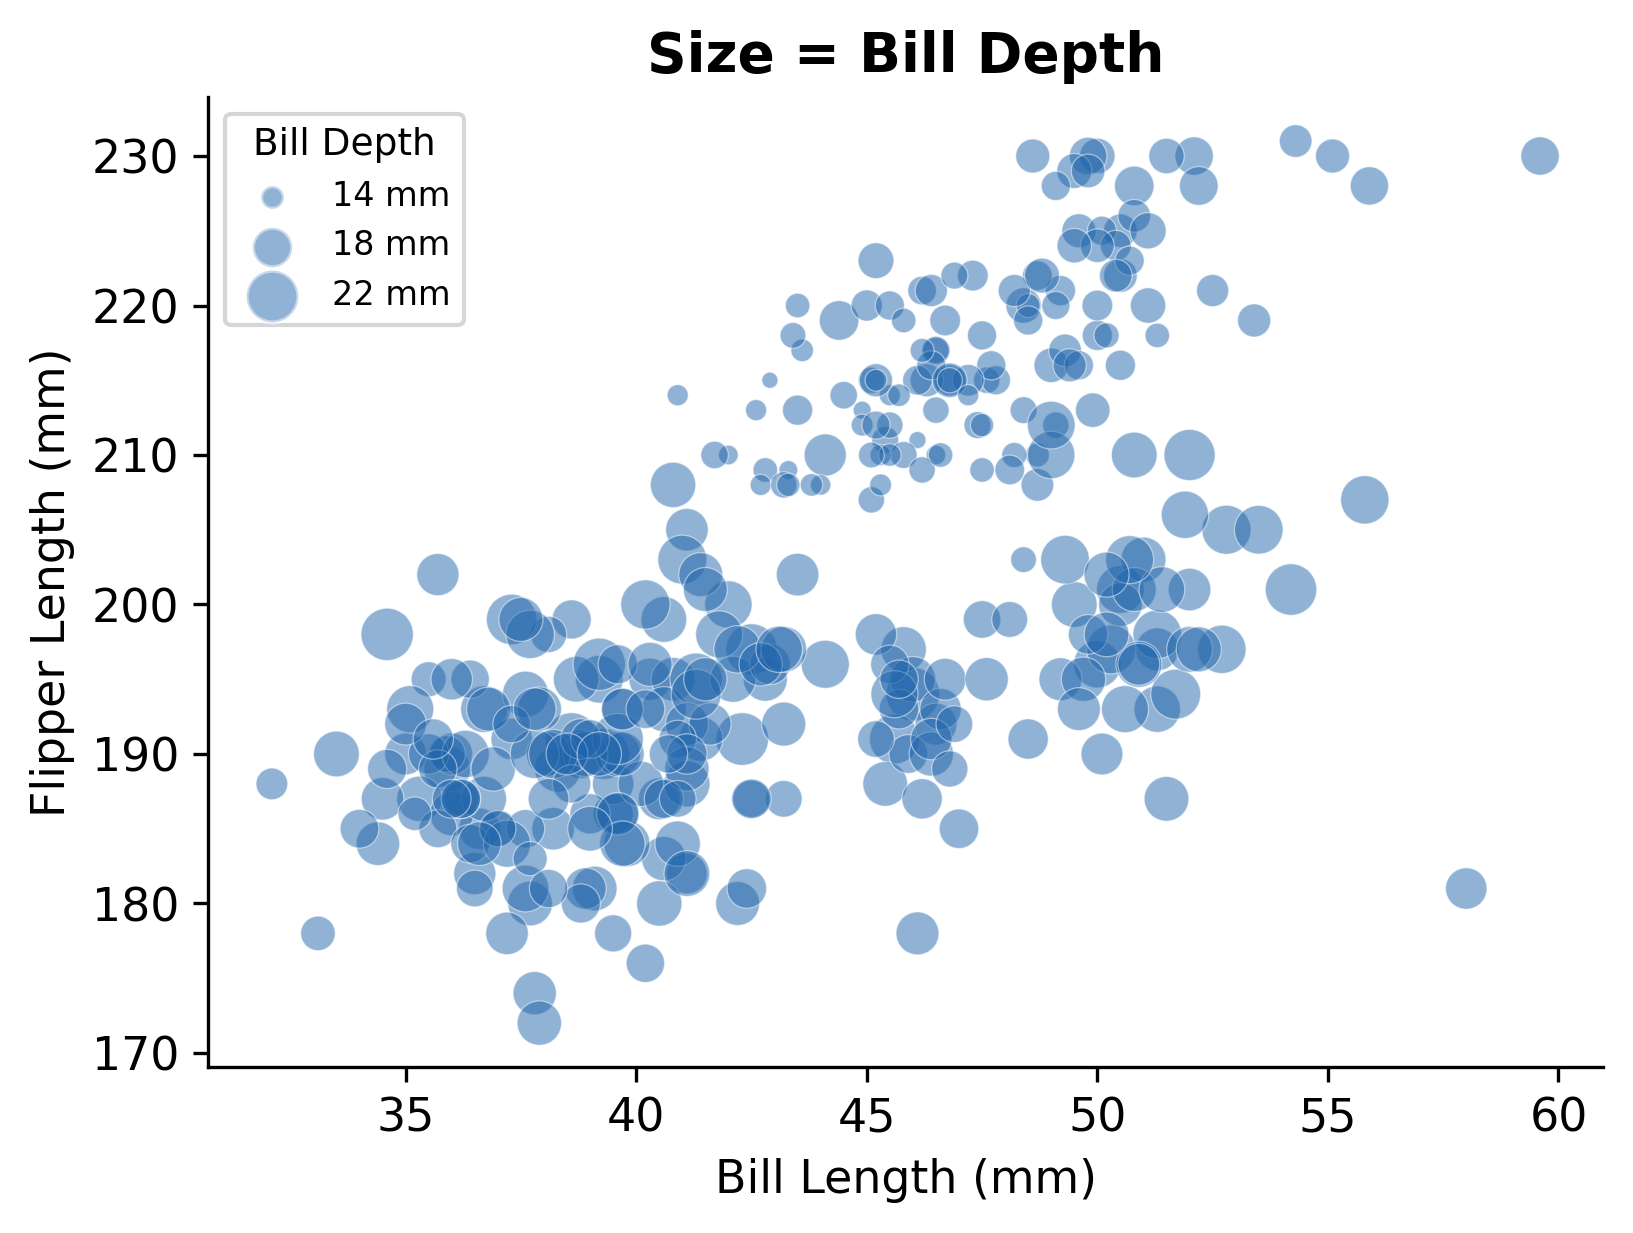
\includegraphics[width=\textwidth]{m1_5_size.png}
\begin{alertblock}{Pro-Tip}
    \scriptsize Always set \texttt{range = c(1, 5)} (R) or \texttt{range=(1,5)} (Python) to control the min/max point size. The default range is often too narrow.
\end{alertblock}
\end{column}
\end{columns}
\end{frame}

% ── 135 ──
\begin{frame}[fragile]{Size --- \Rlang}\smark{135/300}
\begin{columns}[T]
\begin{column}{0.55\textwidth}
\begin{lstlisting}[style=Rstyle]
ggplot(penguins,
  aes(bill_length_mm,
      flipper_length_mm,
      size = bill_depth_mm)) +
  geom_point(color = "#2166AC",
             alpha = 0.5) +
  scale_size_continuous(
    range = c(1, 6)) +
  labs(size="Bill Depth (mm)") +
  theme_minimal()
\end{lstlisting}
\end{column}
\begin{column}{0.42\textwidth}
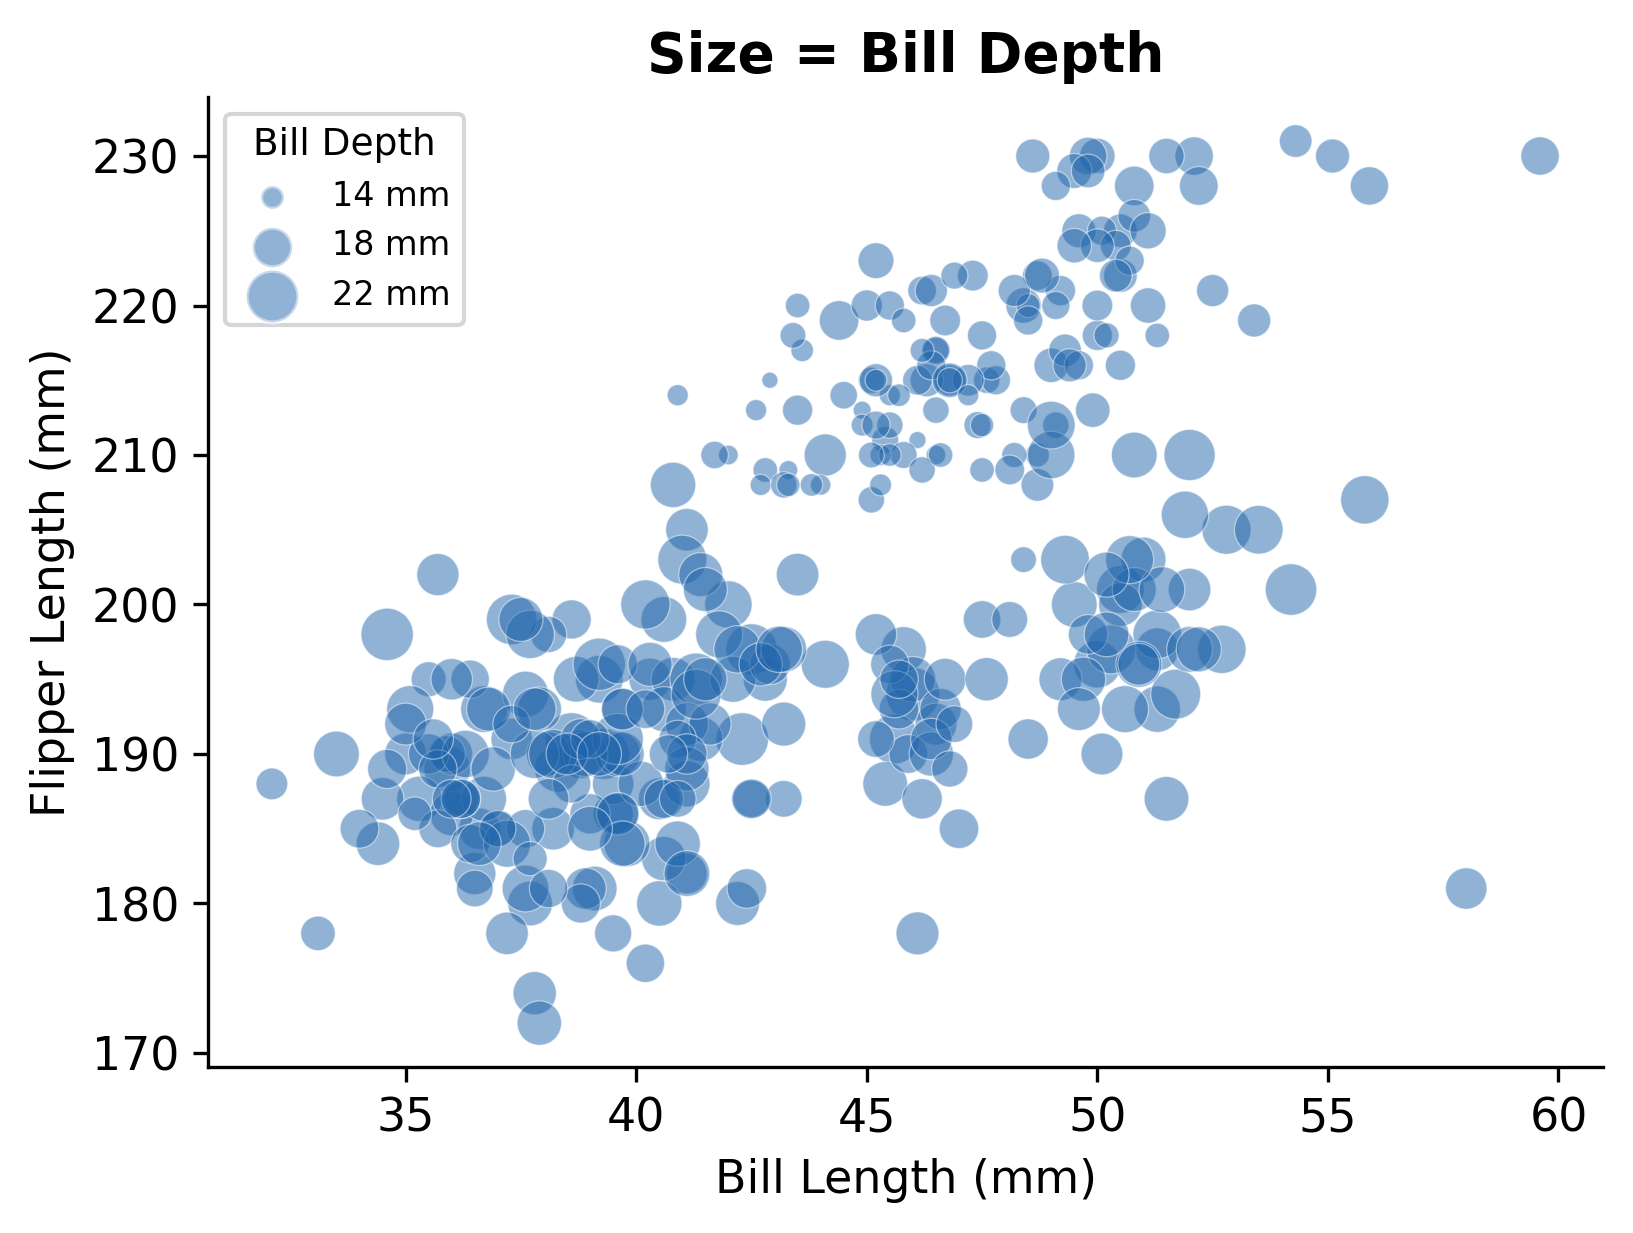
\includegraphics[width=\textwidth]{m1_5_size.png}
\begin{exampleblock}{Data Insight}
    \scriptsize \texttt{scale\_size\_continuous()} maps to \textbf{radius}. For perceptually correct area scaling, use \texttt{scale\_size\_area()} instead.
\end{exampleblock}
\end{column}
\end{columns}
\end{frame}

% ── 136 ──
\begin{frame}[fragile]{Size --- \Python}\smark{136/300}
\begin{columns}[T]
\begin{column}{0.55\textwidth}
\begin{lstlisting}[style=Pystyle]
# plotnine
(ggplot(penguins,
   aes("bill_length_mm",
       "flipper_length_mm",
       size="bill_depth_mm"))
 + geom_point(color="#B2182B",
              alpha=0.5)
 + scale_size_continuous(
     range=(1, 6)))

# matplotlib: s= parameter
ax.scatter(x, y,
    s=depth * 5,  # manual scaling
    alpha=0.5, color="#B2182B")
\end{lstlisting}
\end{column}
\begin{column}{0.42\textwidth}
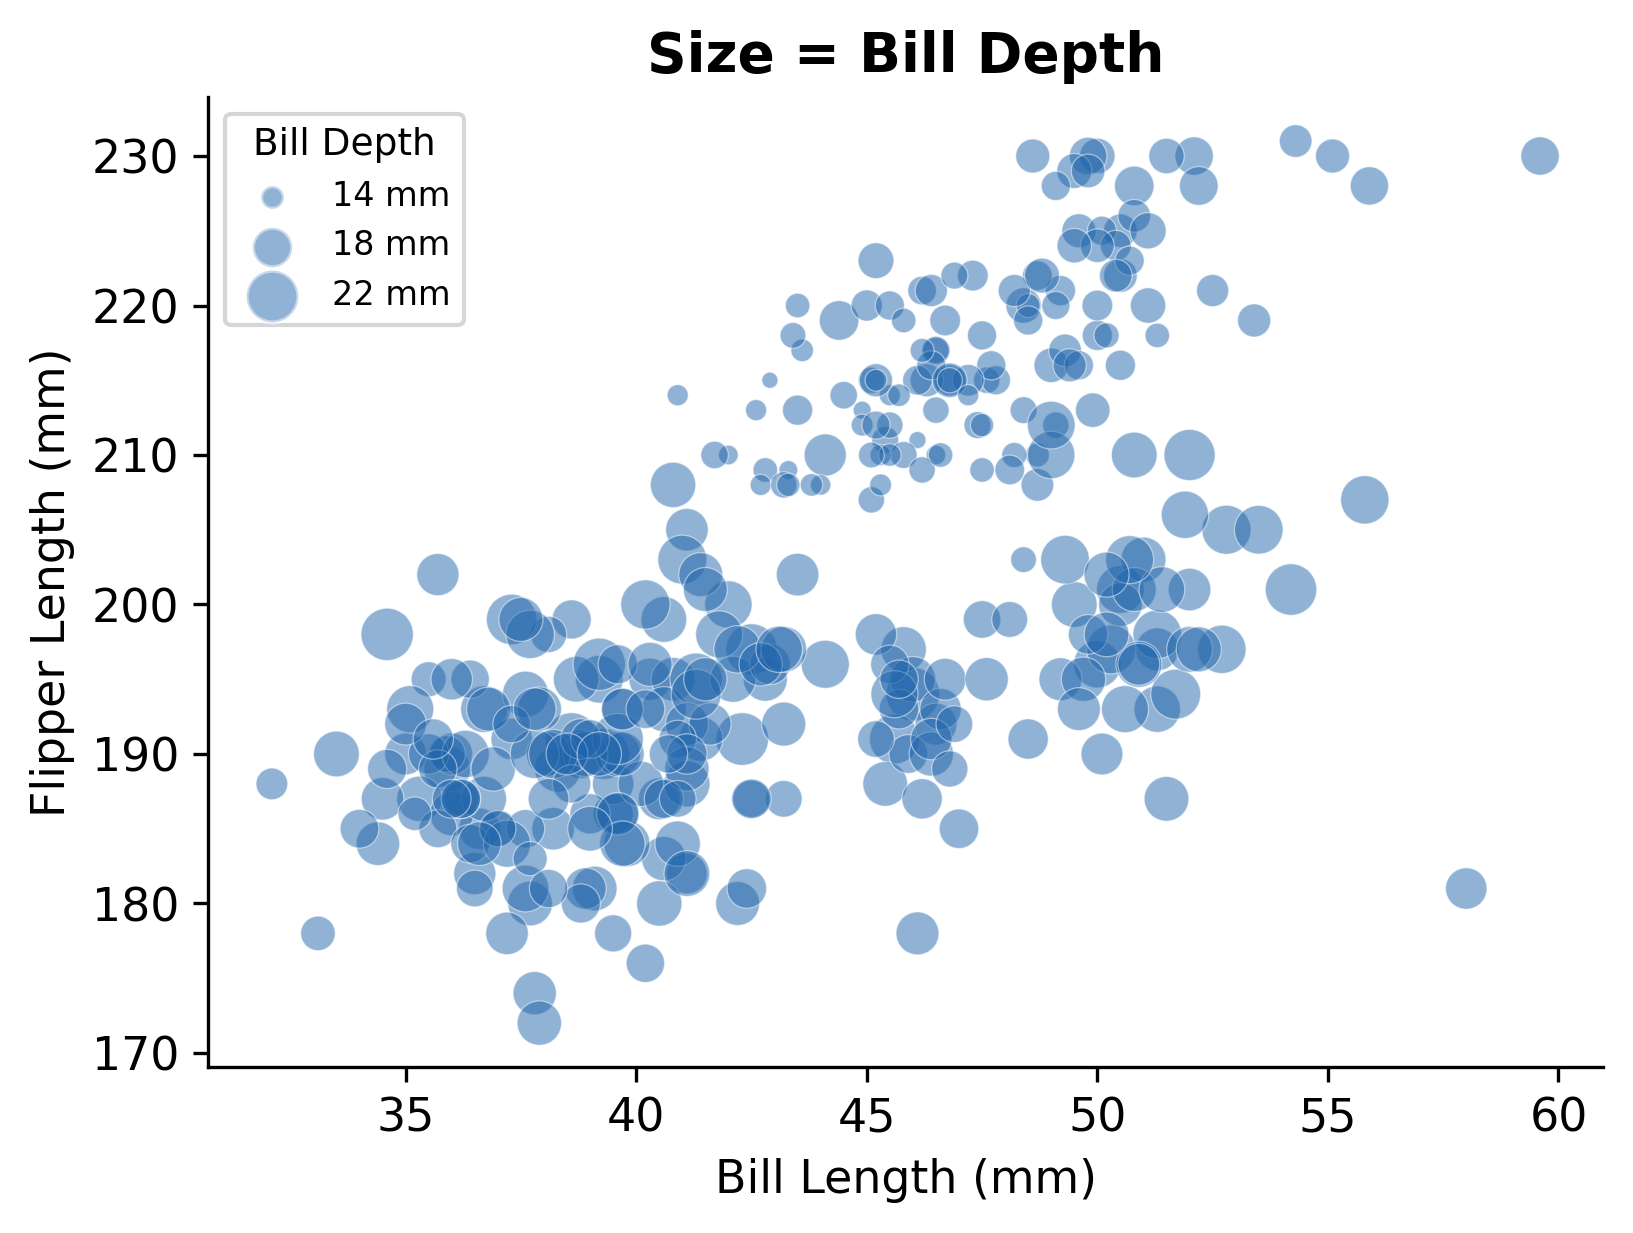
\includegraphics[width=\textwidth]{m1_5_size.png}
\begin{alertblock}{Pro-Tip}
    \scriptsize matplotlib's \texttt{s=} is in \textbf{points$^2$} (area). Double the value $\to$ double the area, which is perceptually correct.
\end{alertblock}
\end{column}
\end{columns}
\end{frame}

% ── 137 ──
\begin{frame}{Alpha Transparency}
\smark{137/300}
\centering
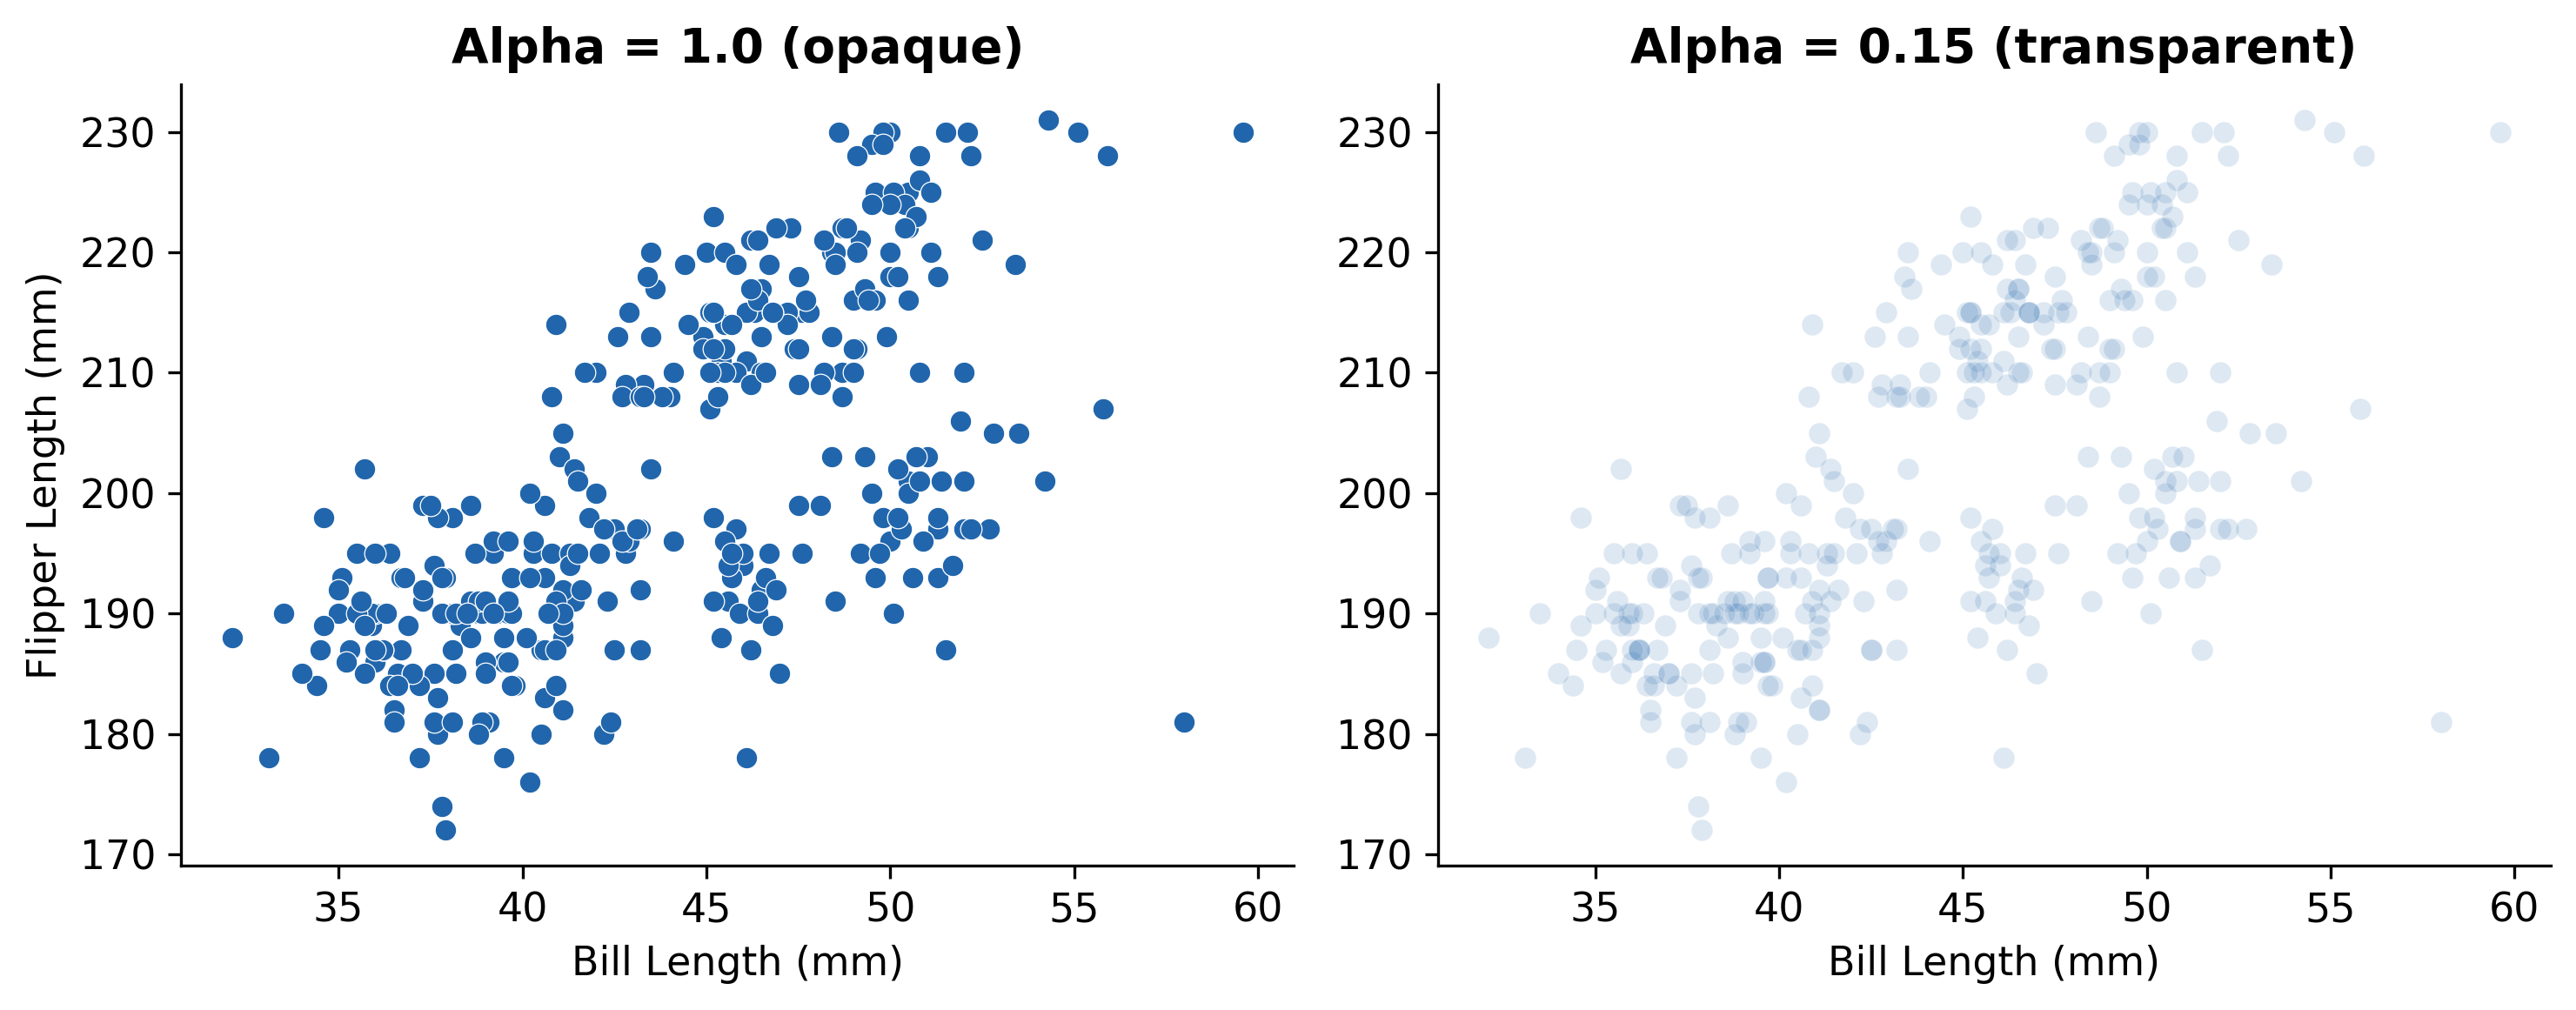
\includegraphics[width=0.85\textwidth]{m1_5_alpha.png}

\vspace{0.2cm}
\begin{columns}[T]
\begin{column}{0.48\textwidth}
\begin{itemize}
    \item Maps to \textbf{opacity} (0 = invisible, 1 = opaque)
    \item Primary use: reveal \textbf{density} in overplotted scatter
    \item Secondary: de-emphasize context data
\end{itemize}
\end{column}
\begin{column}{0.48\textwidth}
\begin{exampleblock}{Data Insight}
    \scriptsize At $\alpha=0.15$, single points are barely visible. Dense clusters darken through additive blending, revealing the true density landscape.
\end{exampleblock}
\end{column}
\end{columns}
\end{frame}

% ── 138 ──
\begin{frame}[fragile]{Alpha --- \Rlang\ and \Python}\smark{138/300}
\begin{columns}[T]
\begin{column}{0.48\textwidth}
\begin{lstlisting}[style=Rstyle]
# Constant alpha (setting)
geom_point(alpha = 0.2)

# Data-driven alpha (mapping)
ggplot(df, aes(x, y,
  alpha = confidence)) +
  geom_point() +
  scale_alpha(range = c(0.1, 1))
\end{lstlisting}
\end{column}
\begin{column}{0.48\textwidth}
\begin{lstlisting}[style=Pystyle]
# Constant alpha
ax.scatter(x, y, alpha=0.2)

# Data-driven alpha (plotnine)
(ggplot(df, aes("x","y",
    alpha="confidence"))
 + geom_point()
 + scale_alpha(range=(0.1, 1)))
\end{lstlisting}
\end{column}
\end{columns}
\vspace{0.2cm}
\begin{alertblock}{Pro-Tip}
    \scriptsize Data-driven alpha is rarely useful except in specialized contexts (e.g., fading old vs.\ new observations). Constant alpha is the common case.
\end{alertblock}
\end{frame}

% ── 139 ──
\begin{frame}{Combining Multiple Aesthetics}
\smark{139/300}
\centering
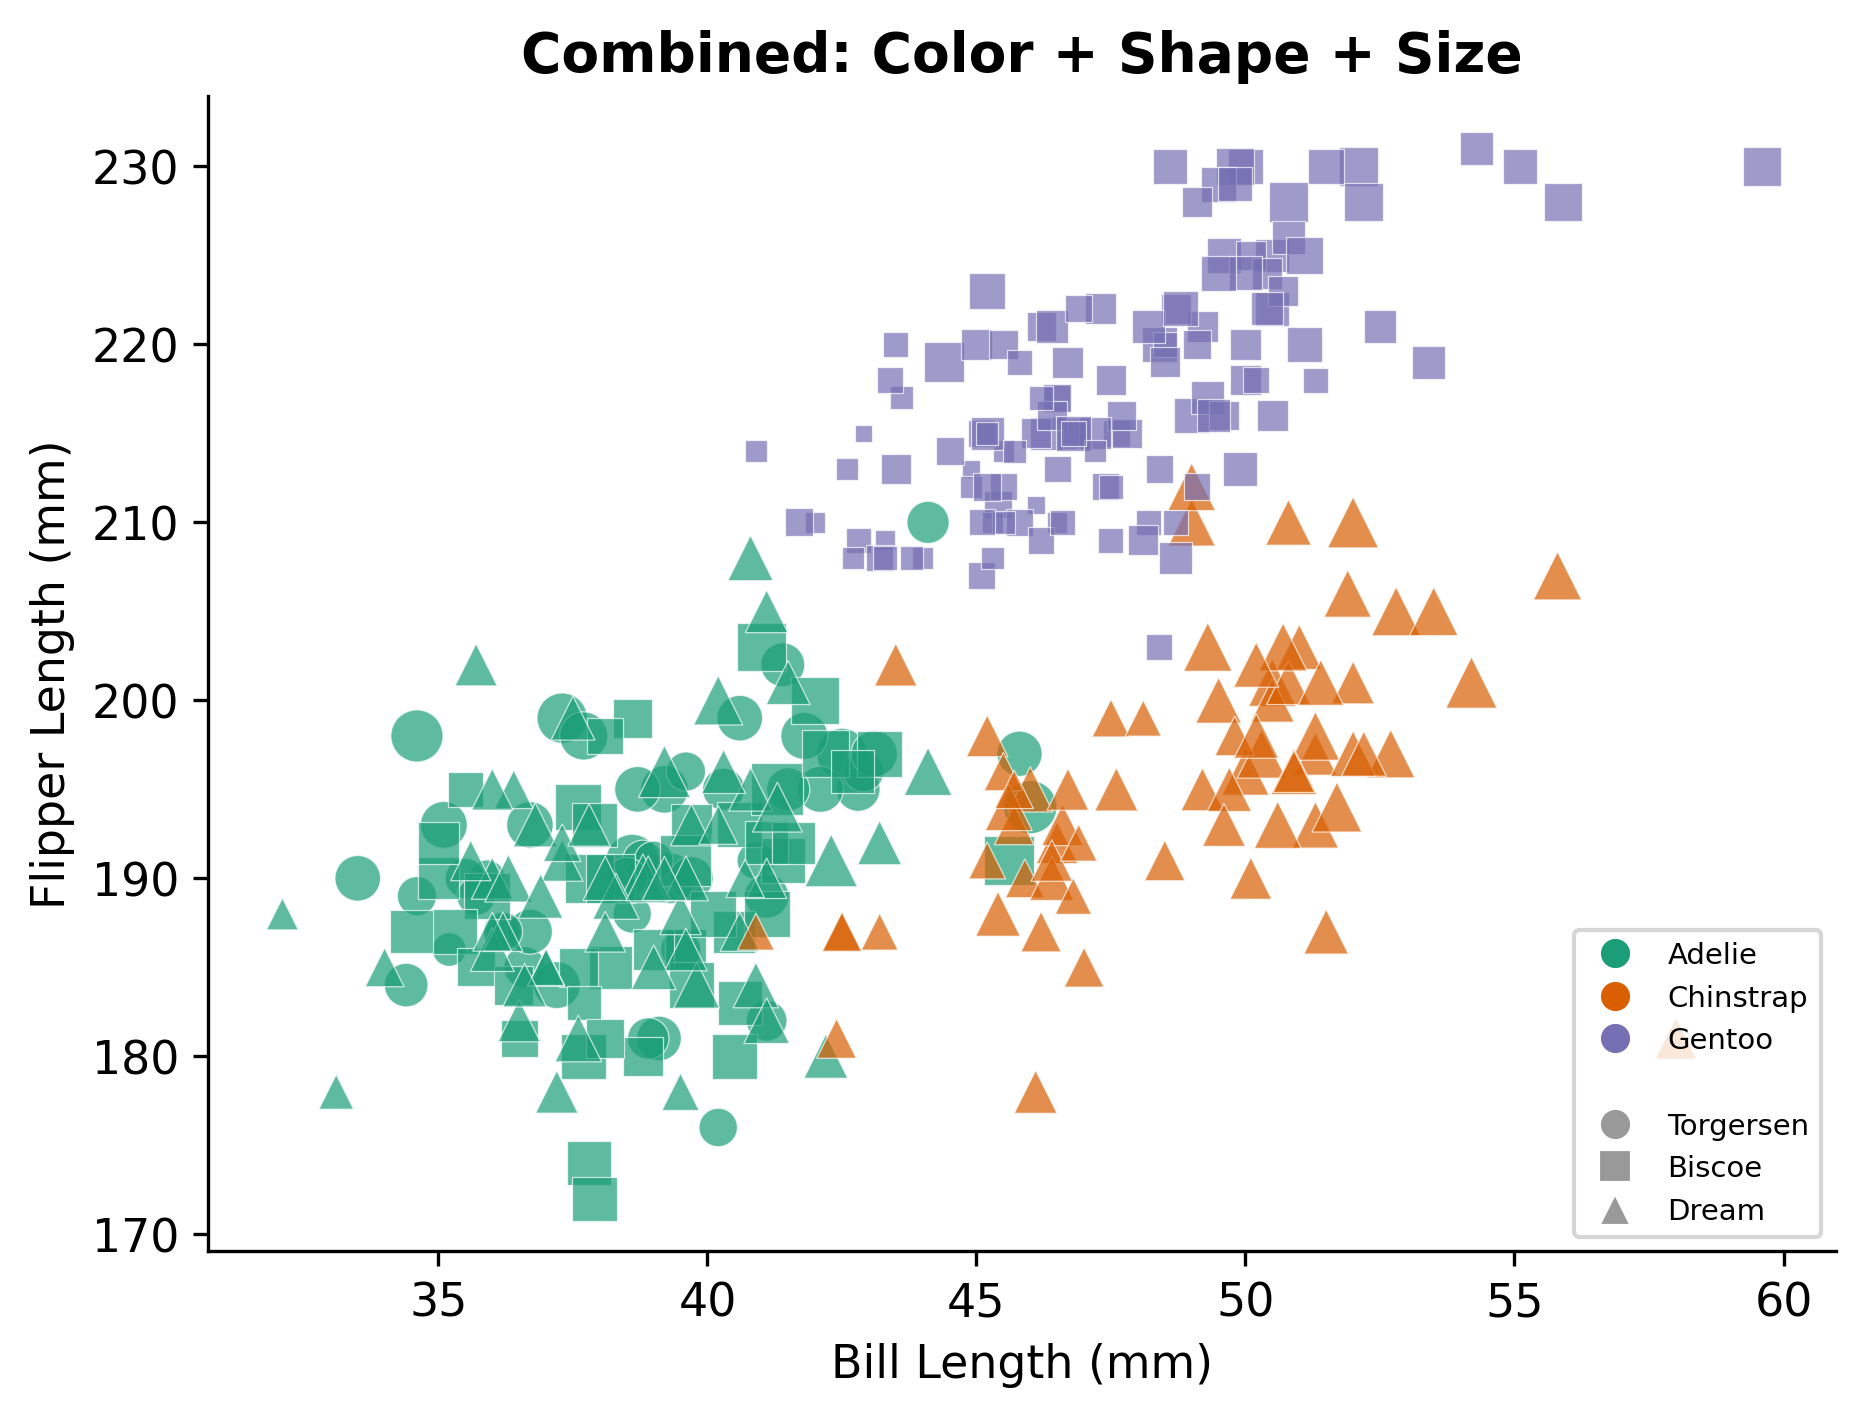
\includegraphics[width=0.68\textwidth]{m1_5_combined.png}

\vspace{0.2cm}
\begin{exampleblock}{Data Insight}
    \scriptsize 5 variables encoded: $x$ = bill length, $y$ = flipper length, color = species, shape = island, size = bill depth. The plot is rich but approaching the legibility ceiling.
\end{exampleblock}
\end{frame}

% ── 140 ──
\begin{frame}[fragile]{Combined Aesthetics --- \Rlang}\smark{140/300}
\begin{columns}[T]
\begin{column}{0.55\textwidth}
\begin{lstlisting}[style=Rstyle]
ggplot(penguins,
  aes(x = bill_length_mm,
      y = flipper_length_mm,
      color = species,
      shape = island,
      size = bill_depth_mm)) +
  geom_point(alpha = 0.7) +
  scale_size_continuous(
    range = c(1, 5)) +
  scale_color_manual(
    values=c("#1B9E77","#D95F02",
             "#7570B3")) +
  theme_minimal()
\end{lstlisting}
\end{column}
\begin{column}{0.42\textwidth}
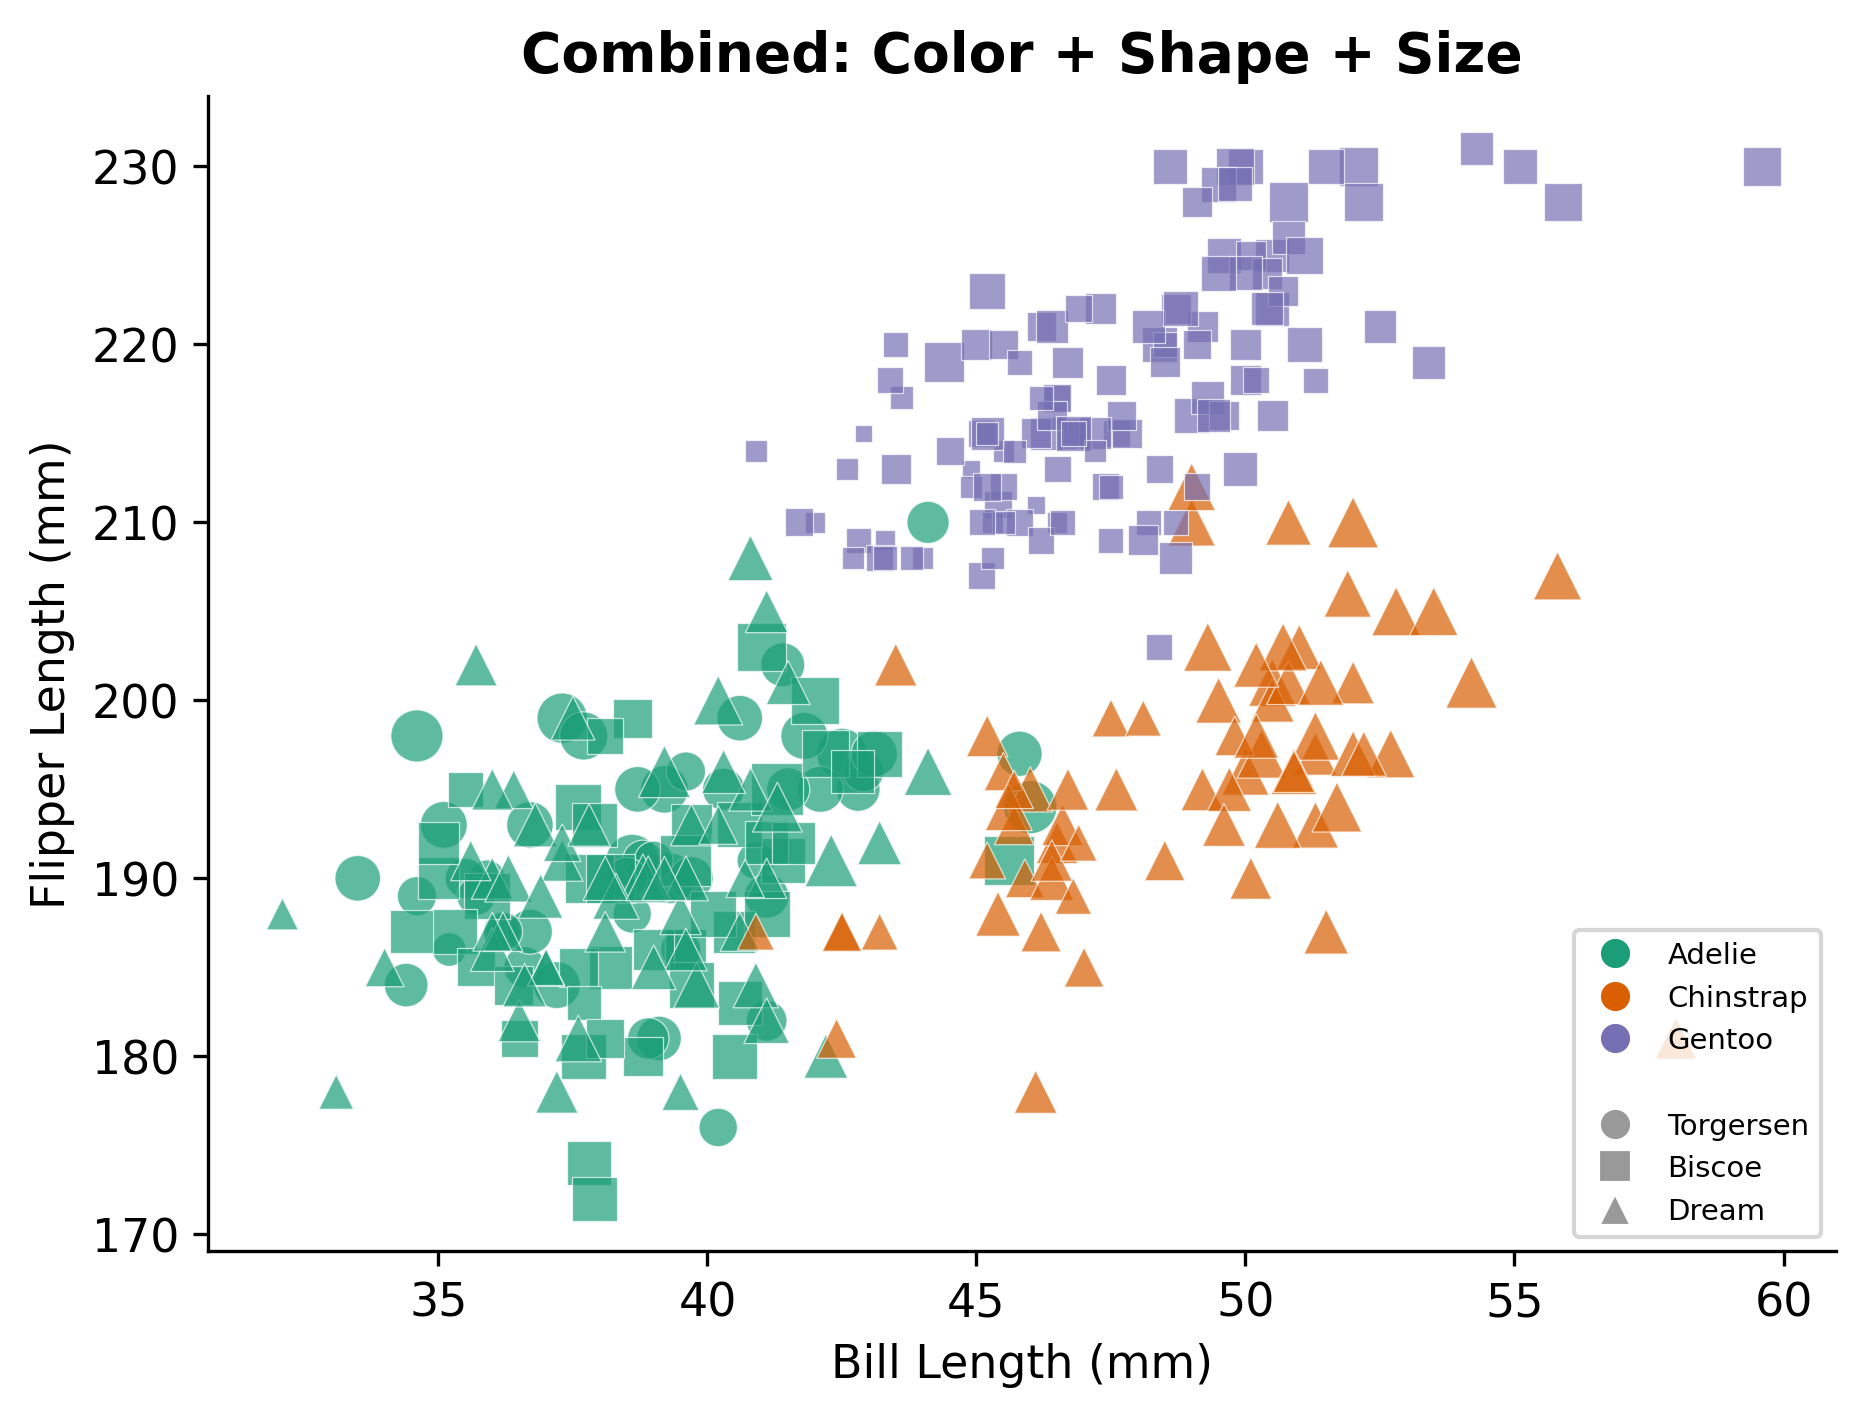
\includegraphics[width=\textwidth]{m1_5_combined.png}
\begin{alertblock}{Pro-Tip}
    \scriptsize Beyond 4 mapped aesthetics, consider \textbf{faceting} instead. A 5-variable scatter is impressive in code but hard for the audience to decode.
\end{alertblock}
\end{column}
\end{columns}
\end{frame}

% ── 141 ──
\begin{frame}[fragile]{Combined Aesthetics --- \Python}\smark{141/300}
\begin{columns}[T]
\begin{column}{0.55\textwidth}
\begin{lstlisting}[style=Pystyle]
(ggplot(penguins,
   aes("bill_length_mm",
       "flipper_length_mm",
       color="species",
       shape="island",
       size="bill_depth_mm"))
 + geom_point(alpha=0.7)
 + scale_size_continuous(
     range=(1, 5))
 + scale_color_manual(
     values=["#1B9E77","#D95F02",
             "#7570B3"]))
\end{lstlisting}
\end{column}
\begin{column}{0.42\textwidth}
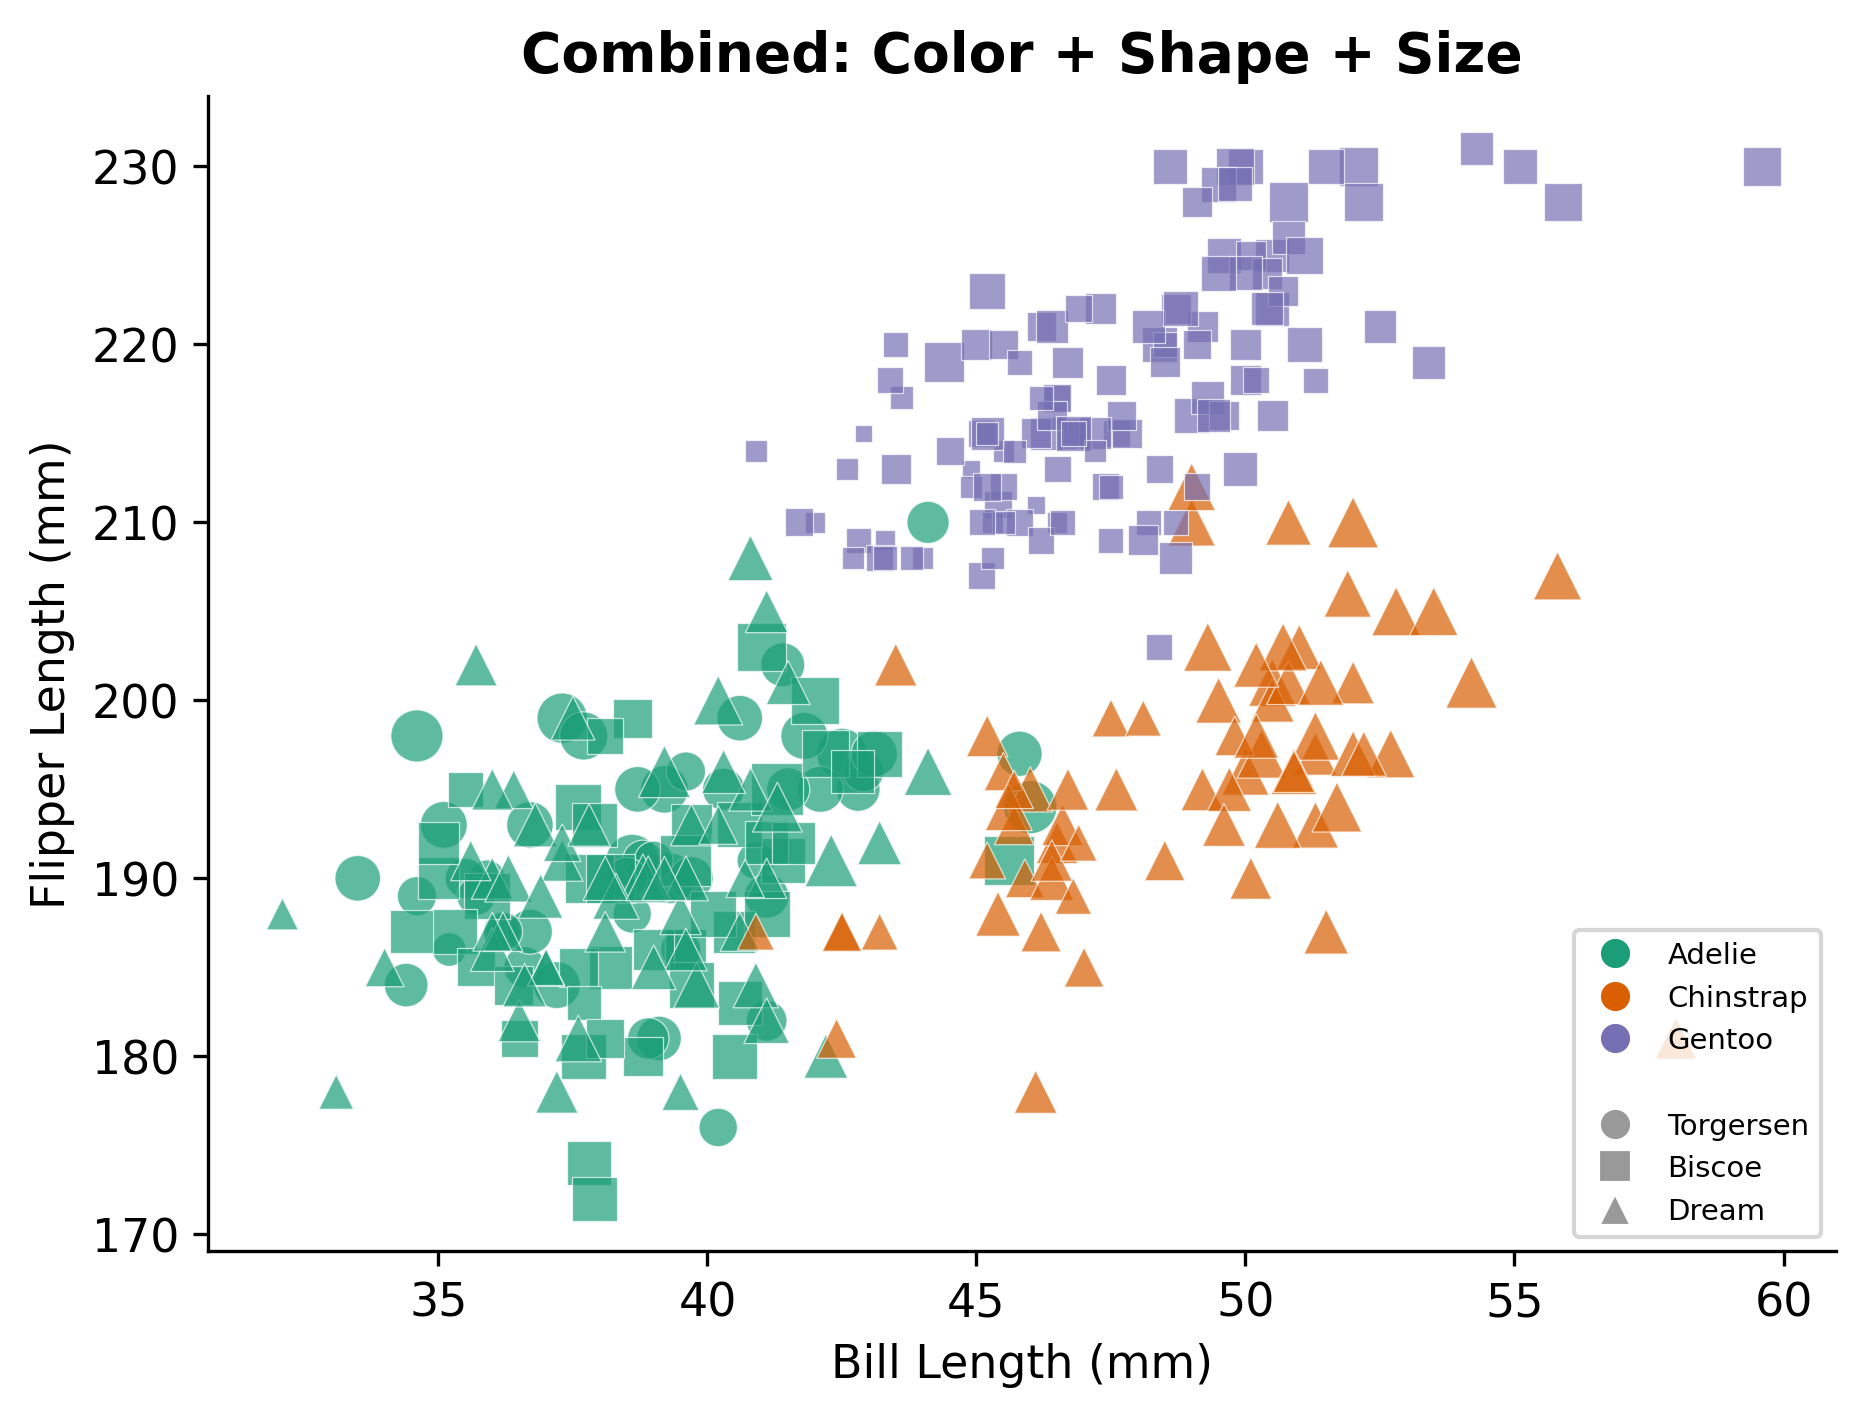
\includegraphics[width=\textwidth]{m1_5_combined.png}
\begin{exampleblock}{Data Insight}
    \scriptsize Identical syntax. The grammar handles 5 aesthetic channels with one function call. matplotlib would require nested loops and manual legend construction.
\end{exampleblock}
\end{column}
\end{columns}
\end{frame}

% ── 142 ──
\begin{frame}{Redundant Encoding: Color + Shape}
\smark{142/300}
\begin{columns}[T]
\begin{column}{0.50\textwidth}
\begin{itemize}
    \item Map the \textbf{same} variable to both color \textbf{and} shape
    \item Provides a second perceptual channel for the same information
    \item Essential for \textbf{accessibility}: colorblind viewers use shape as fallback
    \item No information lost, robustness gained
\end{itemize}
\end{column}
\begin{column}{0.47\textwidth}
\begin{exampleblock}{Data Insight}
    \scriptsize Redundant encoding is not ``wasting a channel'' --- it is insurance. Scientific journals increasingly \textbf{require} shape + color for categorical data.
\end{exampleblock}
\vspace{0.2cm}
\begin{alertblock}{Pro-Tip}
    \scriptsize In ggplot2: \texttt{aes(color=species, shape=species)} gives both. One shared legend is auto-generated.
\end{alertblock}
\end{column}
\end{columns}
\end{frame}

% ── 143 ──
\begin{frame}[fragile]{Redundant Encoding --- Code}\smark{143/300}
\begin{columns}[T]
\begin{column}{0.48\textwidth}
\begin{lstlisting}[style=Rstyle]
# Same variable -> 2 channels
ggplot(penguins,
  aes(bill_length_mm,
      flipper_length_mm,
      color = species,
      shape = species)) +
  geom_point(size = 2.5) +
  scale_color_manual(
    values=c("#1B9E77","#D95F02",
             "#7570B3")) +
  theme_minimal()
# One merged legend appears
\end{lstlisting}
\end{column}
\begin{column}{0.48\textwidth}
\begin{lstlisting}[style=Pystyle]
(ggplot(penguins,
   aes("bill_length_mm",
       "flipper_length_mm",
       color="species",
       shape="species"))
 + geom_point(size=2.5)
 + scale_color_manual(
     values=["#1B9E77","#D95F02",
             "#7570B3"]))
# Merged legend in plotnine too
\end{lstlisting}
\end{column}
\end{columns}
\end{frame}

% ── 144 ──
\begin{frame}{Colorblind Safety}
\smark{144/300}
\centering
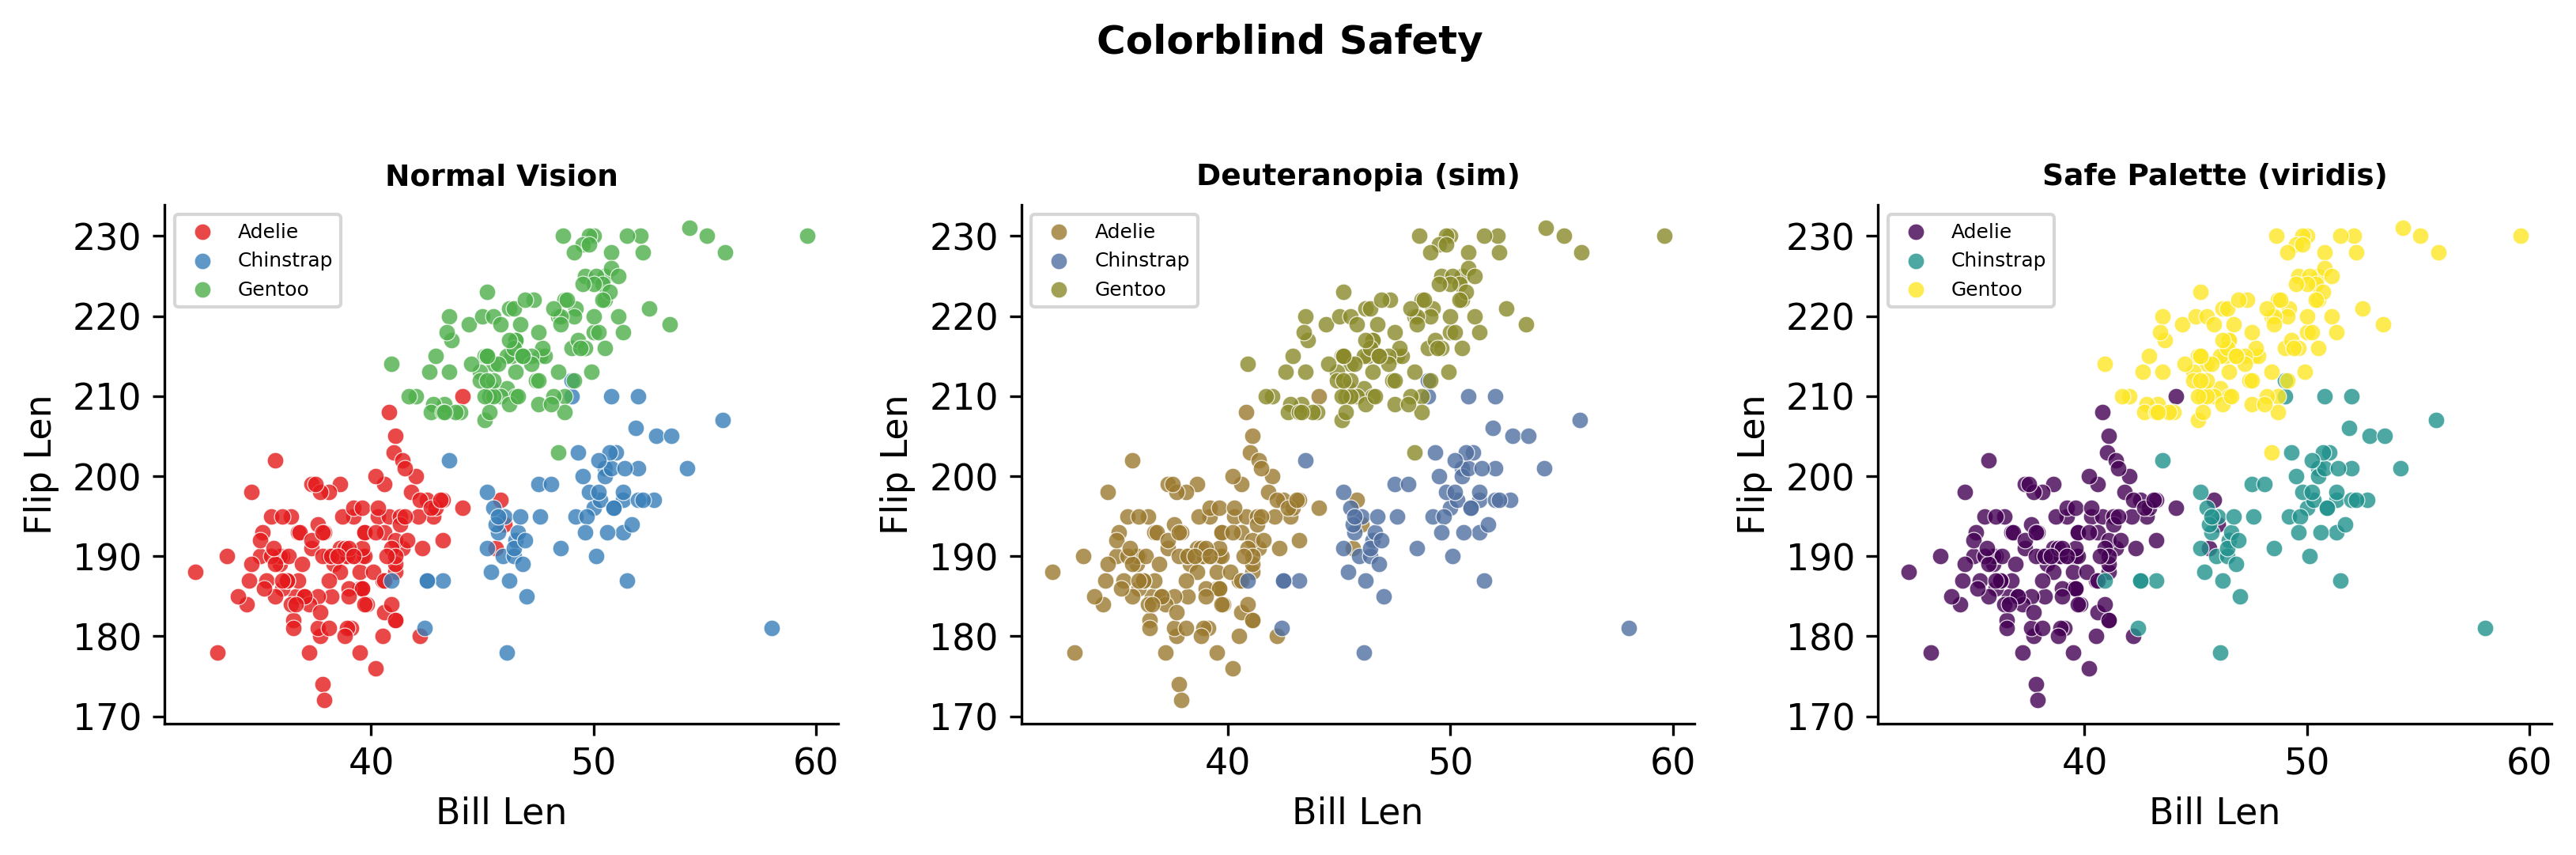
\includegraphics[width=0.92\textwidth]{m1_5_colorblind.png}

\vspace{0.2cm}
\begin{columns}[T]
\begin{column}{0.48\textwidth}
\begin{itemize}
    \item $\sim$8\% of males, $\sim$0.5\% of females have color vision deficiency
    \item Red--green confusion (deuteranopia) is most common
    \item Test every palette with a simulator
\end{itemize}
\end{column}
\begin{column}{0.48\textwidth}
\begin{alertblock}{Pro-Tip}
    \scriptsize Safe defaults: \texttt{viridis}, \texttt{cividis}, \texttt{okabe\_ito}. Avoid red-vs-green without a second channel. R: \texttt{colorblindr::cvd\_grid()}. Python: \texttt{colorspacious}.
\end{alertblock}
\end{column}
\end{columns}
\end{frame}

% ── 145 ──
\begin{frame}[fragile]{Colorblind-Safe Palettes --- Code}\smark{145/300}
\begin{columns}[T]
\begin{column}{0.48\textwidth}
\begin{lstlisting}[style=Rstyle]
# viridis (safe for all types)
scale_color_viridis_d()
scale_fill_viridis_d()

# Okabe-Ito (8 colors)
scale_color_manual(values =
  c("#E69F00","#56B4E9",
    "#009E73","#F0E442",
    "#0072B2","#D55E00",
    "#CC79A7","#999999"))

# Simulate CVD
library(colorblindr)
cvd_grid(my_plot)
\end{lstlisting}
\end{column}
\begin{column}{0.48\textwidth}
\begin{lstlisting}[style=Pystyle]
# viridis in plotnine
scale_color_cmap("viridis")

# Okabe-Ito manual
okabe = ["#E69F00","#56B4E9",
    "#009E73","#F0E442",
    "#0072B2","#D55E00",
    "#CC79A7","#999999"]
scale_color_manual(values=okabe)

# matplotlib
plt.colormaps["cividis"]
\end{lstlisting}
\end{column}
\end{columns}
\end{frame}

% ── 146 ──
\begin{frame}{When Color Fails: Too Many Categories}
\smark{146/300}
\centering
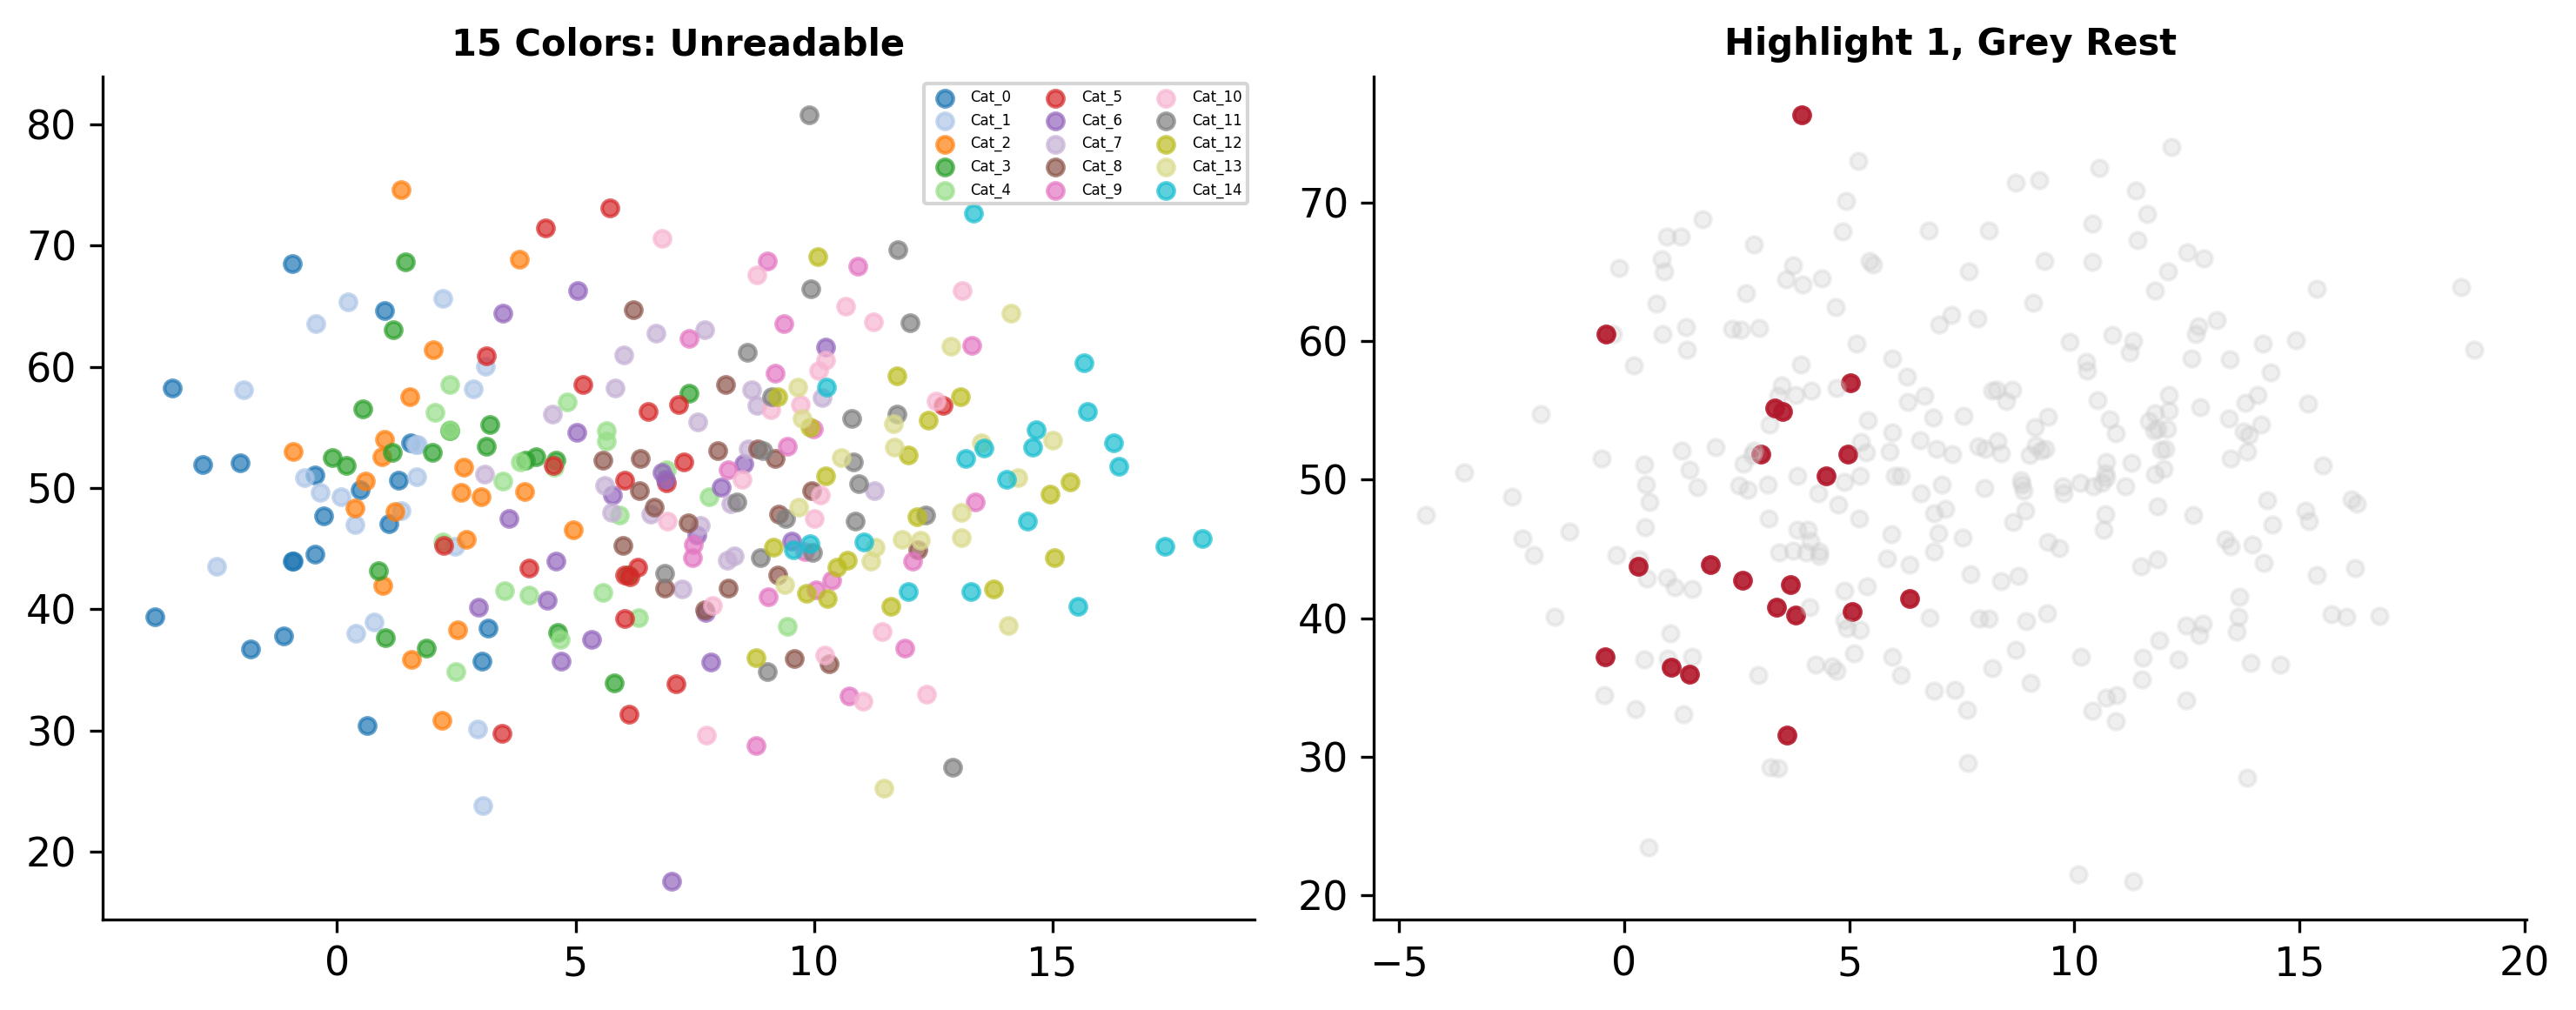
\includegraphics[width=0.88\textwidth]{m1_5_too_many_colors.png}

\vspace{0.2cm}
\begin{exampleblock}{Data Insight}
    \scriptsize Left: 15 colors are indistinguishable. Right: highlight one group, grey out the rest. The reader's eye is drawn exactly where you want.
\end{exampleblock}
\end{frame}

% ── 147 ──
\begin{frame}{The ``Highlight One'' Pattern}
\smark{147/300}
\begin{columns}[T]
\begin{column}{0.50\textwidth}
\begin{itemize}
    \item Color one group in a saturated hue
    \item Set all other groups to light grey ($\alpha = 0.3$)
    \item The highlighted group \textbf{pops out preattentively}
    \item Works for any number of categories
\end{itemize}
\end{column}
\begin{column}{0.47\textwidth}
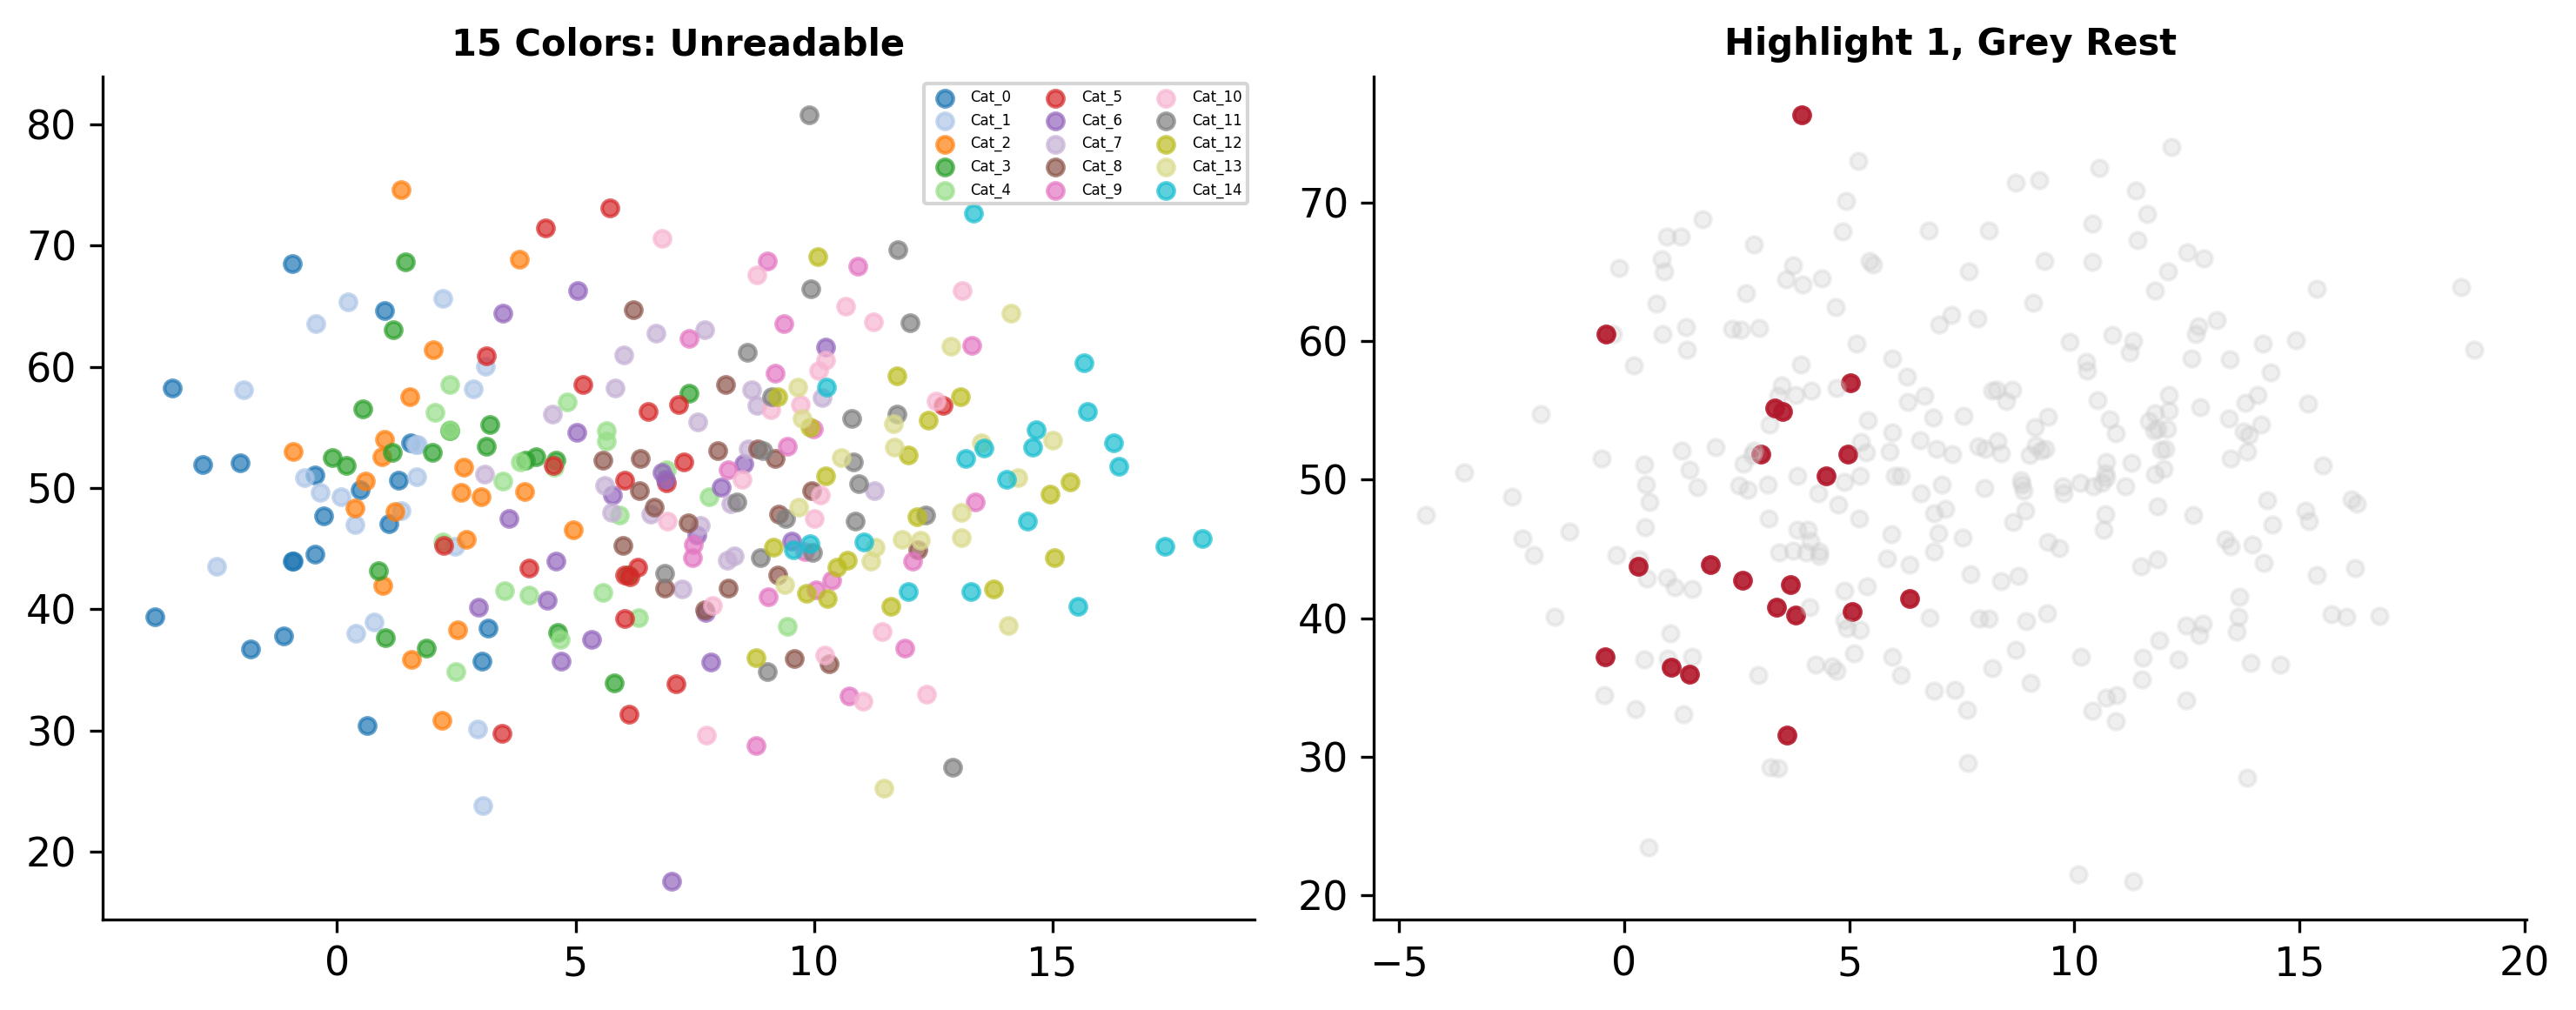
\includegraphics[width=\textwidth]{m1_5_too_many_colors.png}
\begin{alertblock}{Pro-Tip}
    \scriptsize In ggplot2, use \texttt{gghighlight::gghighlight(species == "Gentoo")}. In seaborn, filter + two scatter calls (highlight on top).
\end{alertblock}
\end{column}
\end{columns}
\end{frame}

% ── 148 ──
\begin{frame}[fragile]{Highlight Pattern --- Code}\smark{148/300}
\begin{columns}[T]
\begin{column}{0.48\textwidth}
\begin{lstlisting}[style=Rstyle]
library(gghighlight)

ggplot(penguins,
  aes(bill_length_mm,
      flipper_length_mm,
      color = species)) +
  geom_point(size = 2) +
  gghighlight(
    species == "Gentoo") +
  theme_minimal()
\end{lstlisting}
\end{column}
\begin{column}{0.48\textwidth}
\begin{lstlisting}[style=Pystyle]
# Manual in matplotlib
for sp in species_list:
    sub = pen[pen["species"]==sp]
    if sp == "Gentoo":
        c, a = "#7570B3", 0.9
    else:
        c, a = "#CCCCCC", 0.3
    ax.scatter(sub["x"], sub["y"],
               color=c, alpha=a)
\end{lstlisting}
\end{column}
\end{columns}
\vspace{0.2cm}
\begin{exampleblock}{Data Insight}
    \scriptsize \texttt{gghighlight} is a one-liner in R. In Python, the two-pass pattern (grey all, then overlay target) achieves the same.
\end{exampleblock}
\end{frame}

% ── 149 ──
\begin{frame}{Module 1.5 --- Key Takeaways}\smark{149/300}
\begin{enumerate}
    \item \textbf{Match scale type to variable type.} Sequential for continuous, qualitative for nominal.
    \item \textbf{Shape $\leq$6 levels.} Beyond that, use color or facets.
    \item \textbf{Size encodes area.} Humans underestimate; use \texttt{scale\_size\_area()} for honesty.
    \item \textbf{Redundant encoding} (color + shape) is insurance, not waste.
    \item \textbf{Test for colorblindness.} Default to viridis/cividis/Okabe--Ito.
    \item \textbf{$>$8 categories?} Highlight one, grey the rest.
\end{enumerate}
\end{frame}

% ── 150 ──
\begin{frame}{}\smark{150/300}
\centering\vspace{1.5cm}
{\Large\textbf{Module 1.5 Complete}}\\[0.5cm]
You now control all four non-positional aesthetic channels --- color, shape, size, alpha --- with the right palette for each data type, and know when to \emph{not} use color.\\[0.5cm]
\textbf{Next:} Module 1.6 --- Faceting and Small Multiples.
\end{frame}

% ═══════════════════════════════════════════════════════
%  MODULE 1.6 — Faceting and Small Multiples
% ═══════════════════════════════════════════════════════
\section{Module 1.6 --- Faceting and Small Multiples}

% ── 151 ──
\begin{frame}{Module 1.6 --- Roadmap}\smark{151/300}
\begin{enumerate}
    \item Tufte's ``small multiples'' principle
    \item \texttt{facet\_wrap()}: one variable, 1D strip
    \item \texttt{facet\_grid()}: two variables, 2D matrix
    \item Free vs.\ fixed scales --- and when each is honest
    \item Controlling \texttt{ncol}, \texttt{nrow}, and panel ordering
    \item Small multiples with context (grey background trick)
    \item When faceting fails: too many panels
    \item Faceted distributions, lines, and bars
\end{enumerate}
\end{frame}

% ── 152 ──
\begin{frame}{Tufte's Small Multiples}
\smark{152/300}
\begin{columns}[T]
\begin{column}{0.50\textwidth}
\begin{itemize}
    \item ``Illustrations of postage-stamp size are indexed by category or time'' (Tufte, 1983)
    \item Same plot structure, different data subsets
    \item The eye compares \textbf{across panels} effortlessly because axes, geoms, and scales are identical
    \item An alternative to color when categories exceed 5--6
\end{itemize}
\end{column}
\begin{column}{0.47\textwidth}
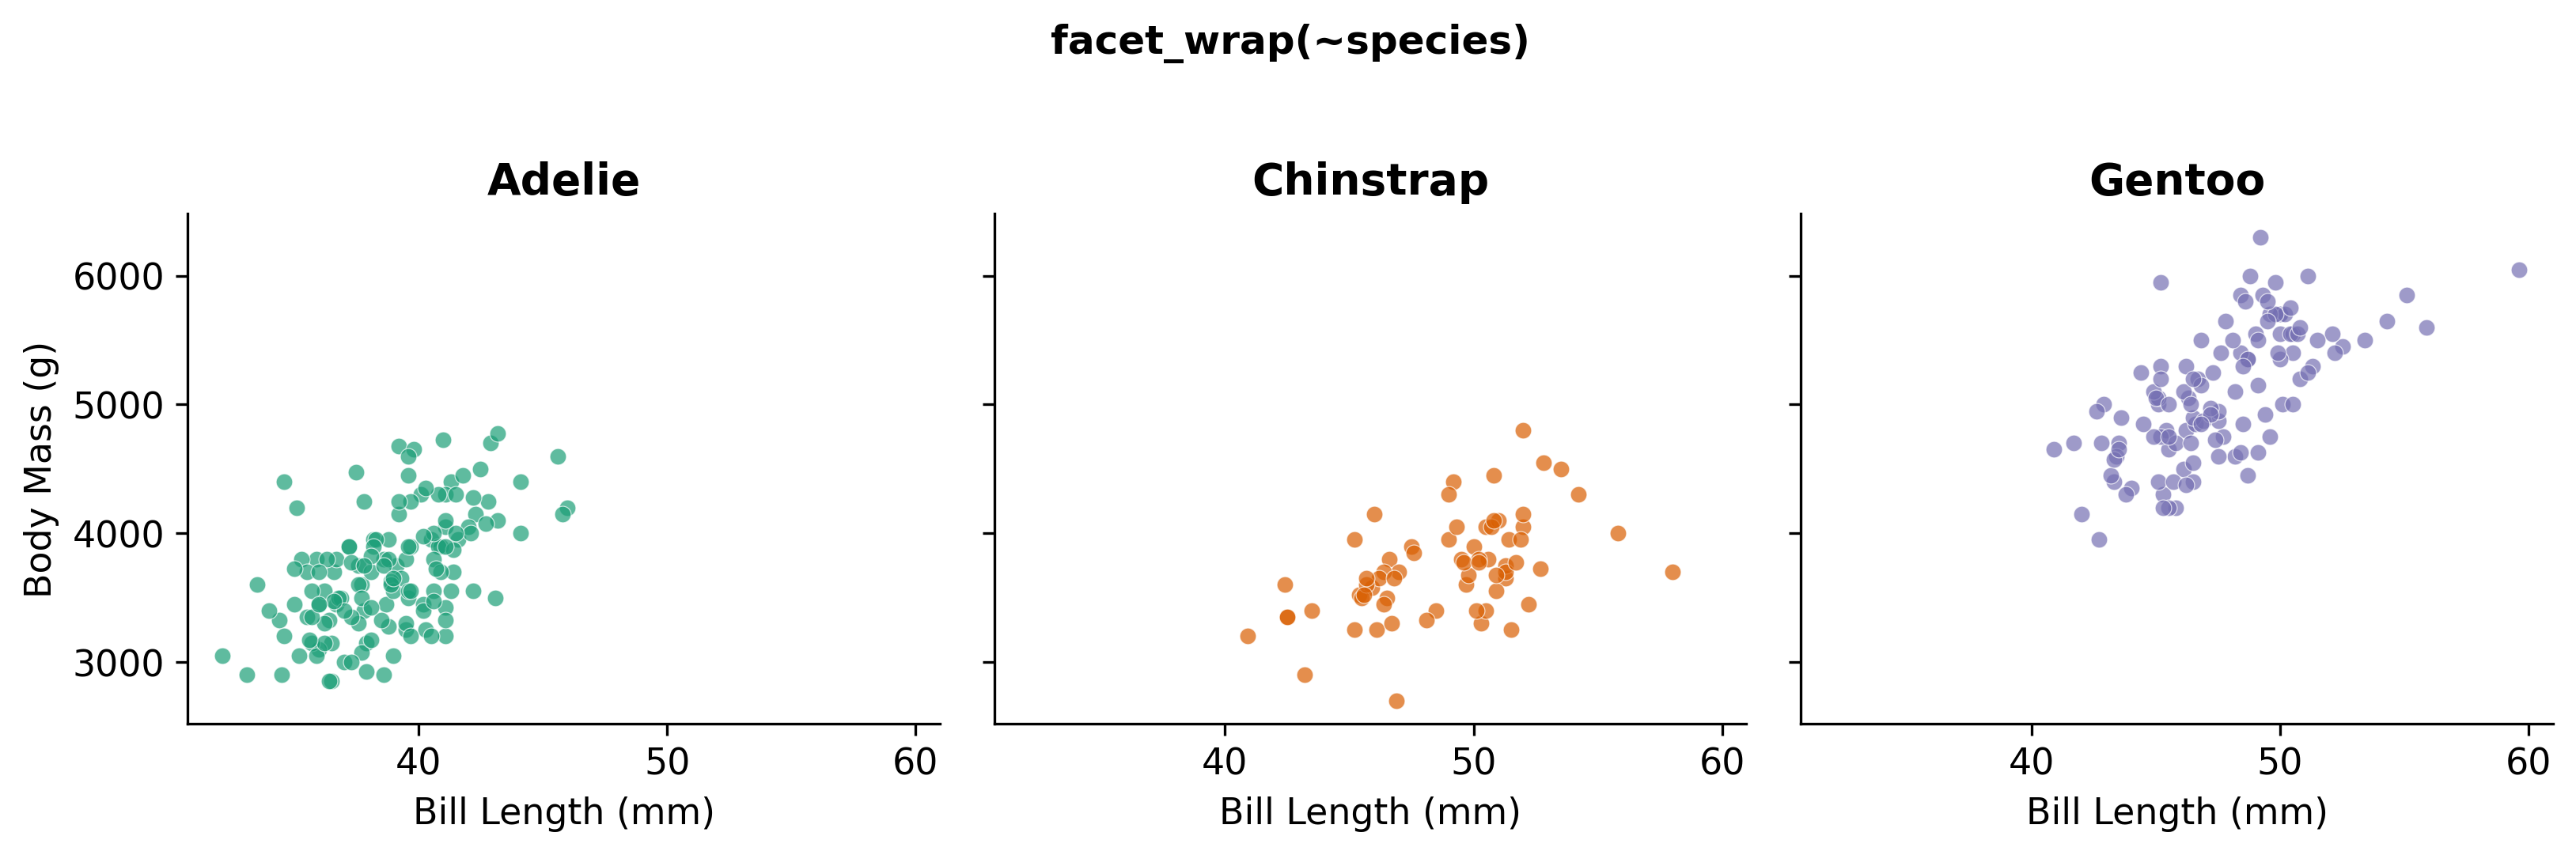
\includegraphics[width=\textwidth]{m1_6_wrap_species.png}
\begin{exampleblock}{Data Insight}
    \scriptsize Each species gets its own panel. No occlusion, no legend decoding. Comparison is done by spatial position.
\end{exampleblock}
\end{column}
\end{columns}
\end{frame}

% ── 153 ──
\begin{frame}{\texttt{facet\_wrap}: One Variable, 1D Strip}
\smark{153/300}
\begin{columns}[T]
\begin{column}{0.50\textwidth}
\begin{itemize}
    \item Wraps panels into rows by \texttt{ncol}
    \item One categorical variable determines the split
    \item Panels are labeled automatically with factor levels
    \item Shared axes by default (same $x$, same $y$)
\end{itemize}
\end{column}
\begin{column}{0.47\textwidth}
\centering\small
\begin{tabular}{@{}ll@{}}
    \toprule
    \textbf{Parameter} & \textbf{Effect} \\
    \midrule
    \texttt{ncol = 2}       & 2 columns, rows wrap \\
    \texttt{nrow = 1}       & Force single row \\
    \texttt{scales = "free"} & Independent axes \\
    \texttt{dir = "v"}      & Fill columns first \\
    \bottomrule
\end{tabular}
\vspace{0.2cm}
\begin{alertblock}{Pro-Tip}
    \scriptsize Default \texttt{dir = "h"} fills rows first (left to right, then down). Use \texttt{dir = "v"} for top-to-bottom filling.
\end{alertblock}
\end{column}
\end{columns}
\end{frame}

% ── 154 ──
\begin{frame}[fragile]{\texttt{facet\_wrap} --- \Rlang}\smark{154/300}
\begin{columns}[T]
\begin{column}{0.55\textwidth}
\begin{lstlisting}[style=Rstyle]
ggplot(penguins,
  aes(bill_length_mm,
      body_mass_g,
      color = species)) +
  geom_point(alpha = 0.7) +
  facet_wrap(~species, ncol = 3) +
  scale_color_manual(
    values = c("#1B9E77",
               "#D95F02",
               "#7570B3")) +
  theme_minimal() +
  theme(legend.position = "none")
\end{lstlisting}
\end{column}
\begin{column}{0.42\textwidth}
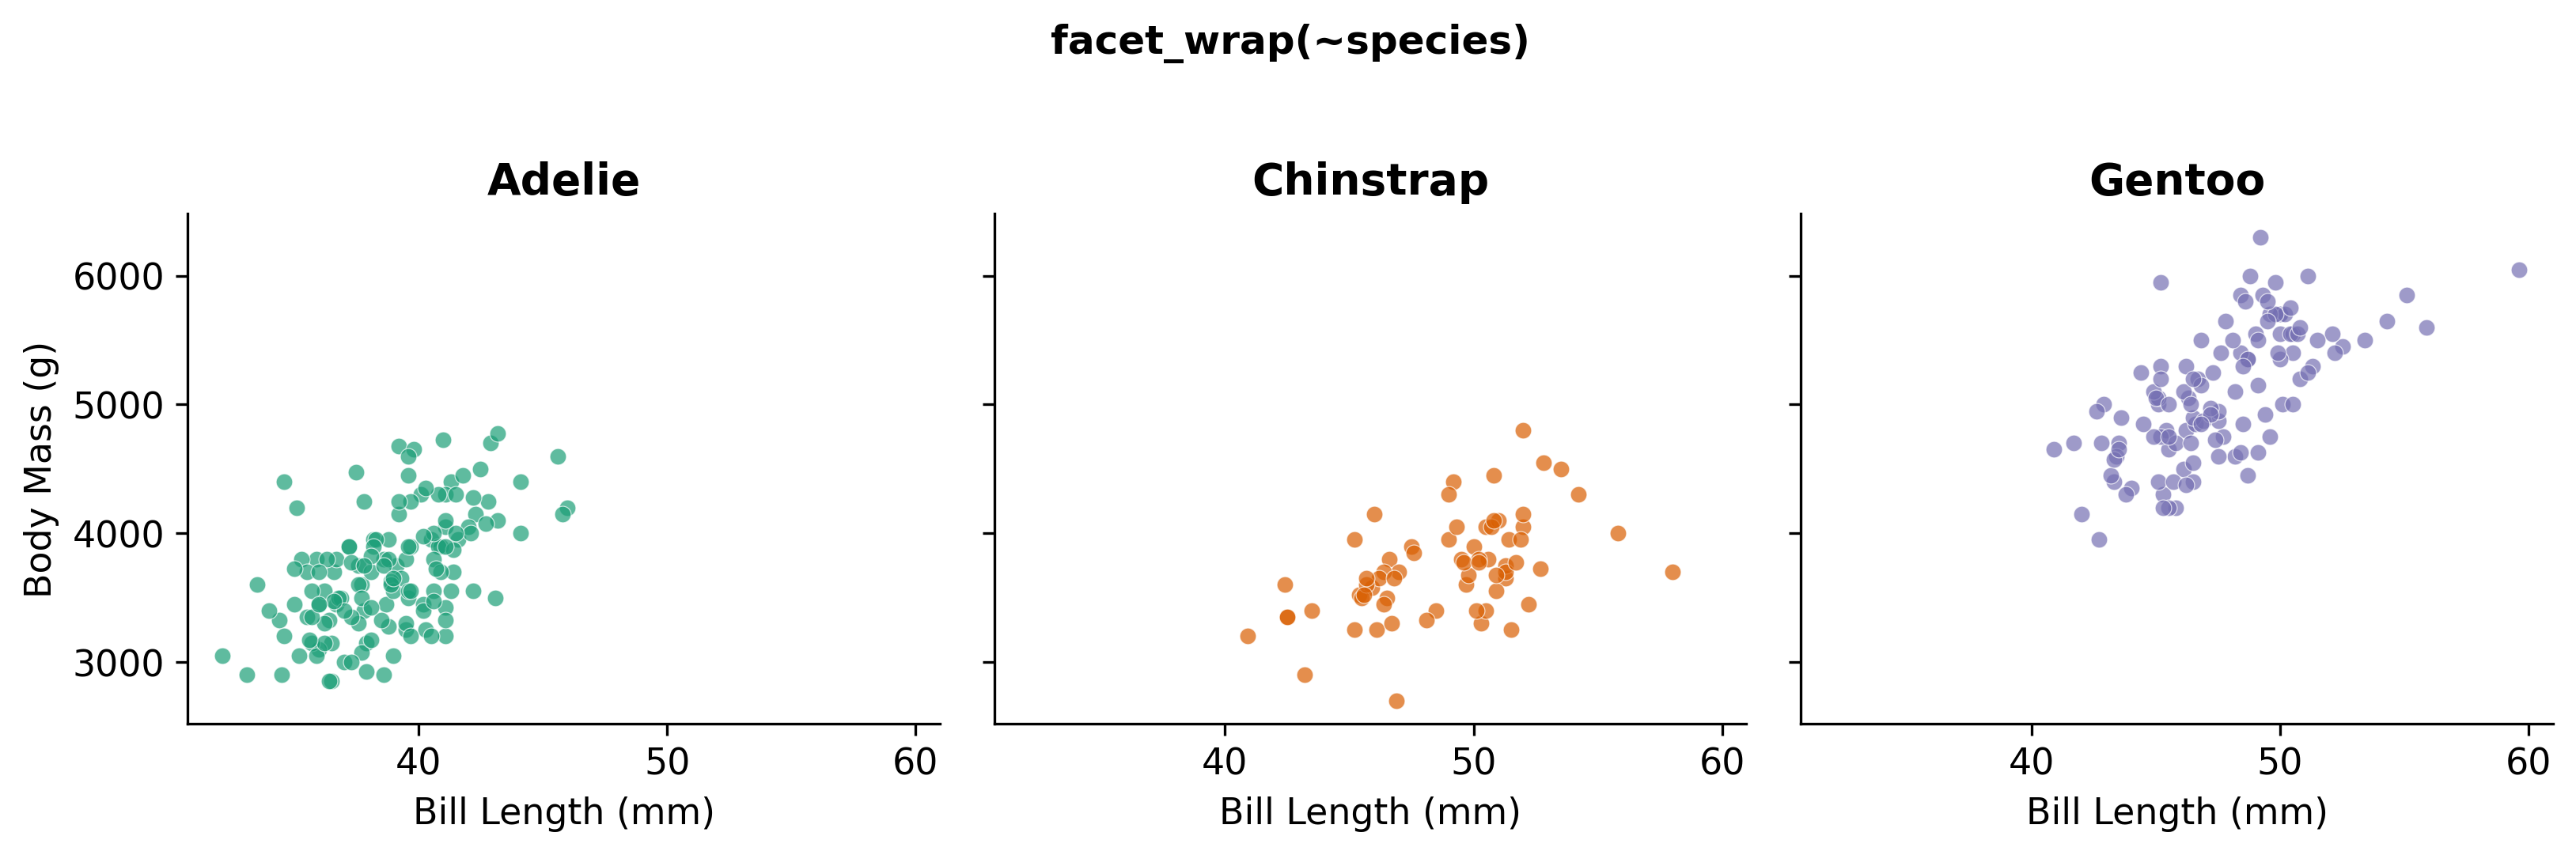
\includegraphics[width=\textwidth]{m1_6_wrap_species.png}
\begin{exampleblock}{Data Insight}
    \scriptsize Legend is redundant when panel titles already label the groups. Remove it with \texttt{legend.position="none"}.
\end{exampleblock}
\end{column}
\end{columns}
\end{frame}

% ── 155 ──
\begin{frame}[fragile]{\texttt{facet\_wrap} --- \Python}\smark{155/300}
\begin{columns}[T]
\begin{column}{0.55\textwidth}
\begin{lstlisting}[style=Pystyle]
# plotnine
(ggplot(penguins,
   aes("bill_length_mm",
       "body_mass_g",
       color="species"))
 + geom_point(alpha=0.7)
 + facet_wrap("~species", ncol=3)
 + theme_minimal()
 + theme(legend_position="none"))

# seaborn FacetGrid
g = sns.FacetGrid(penguins,
    col="species", height=3.5)
g.map_dataframe(sns.scatterplot,
    x="bill_length_mm",
    y="body_mass_g", alpha=0.7)
\end{lstlisting}
\end{column}
\begin{column}{0.42\textwidth}
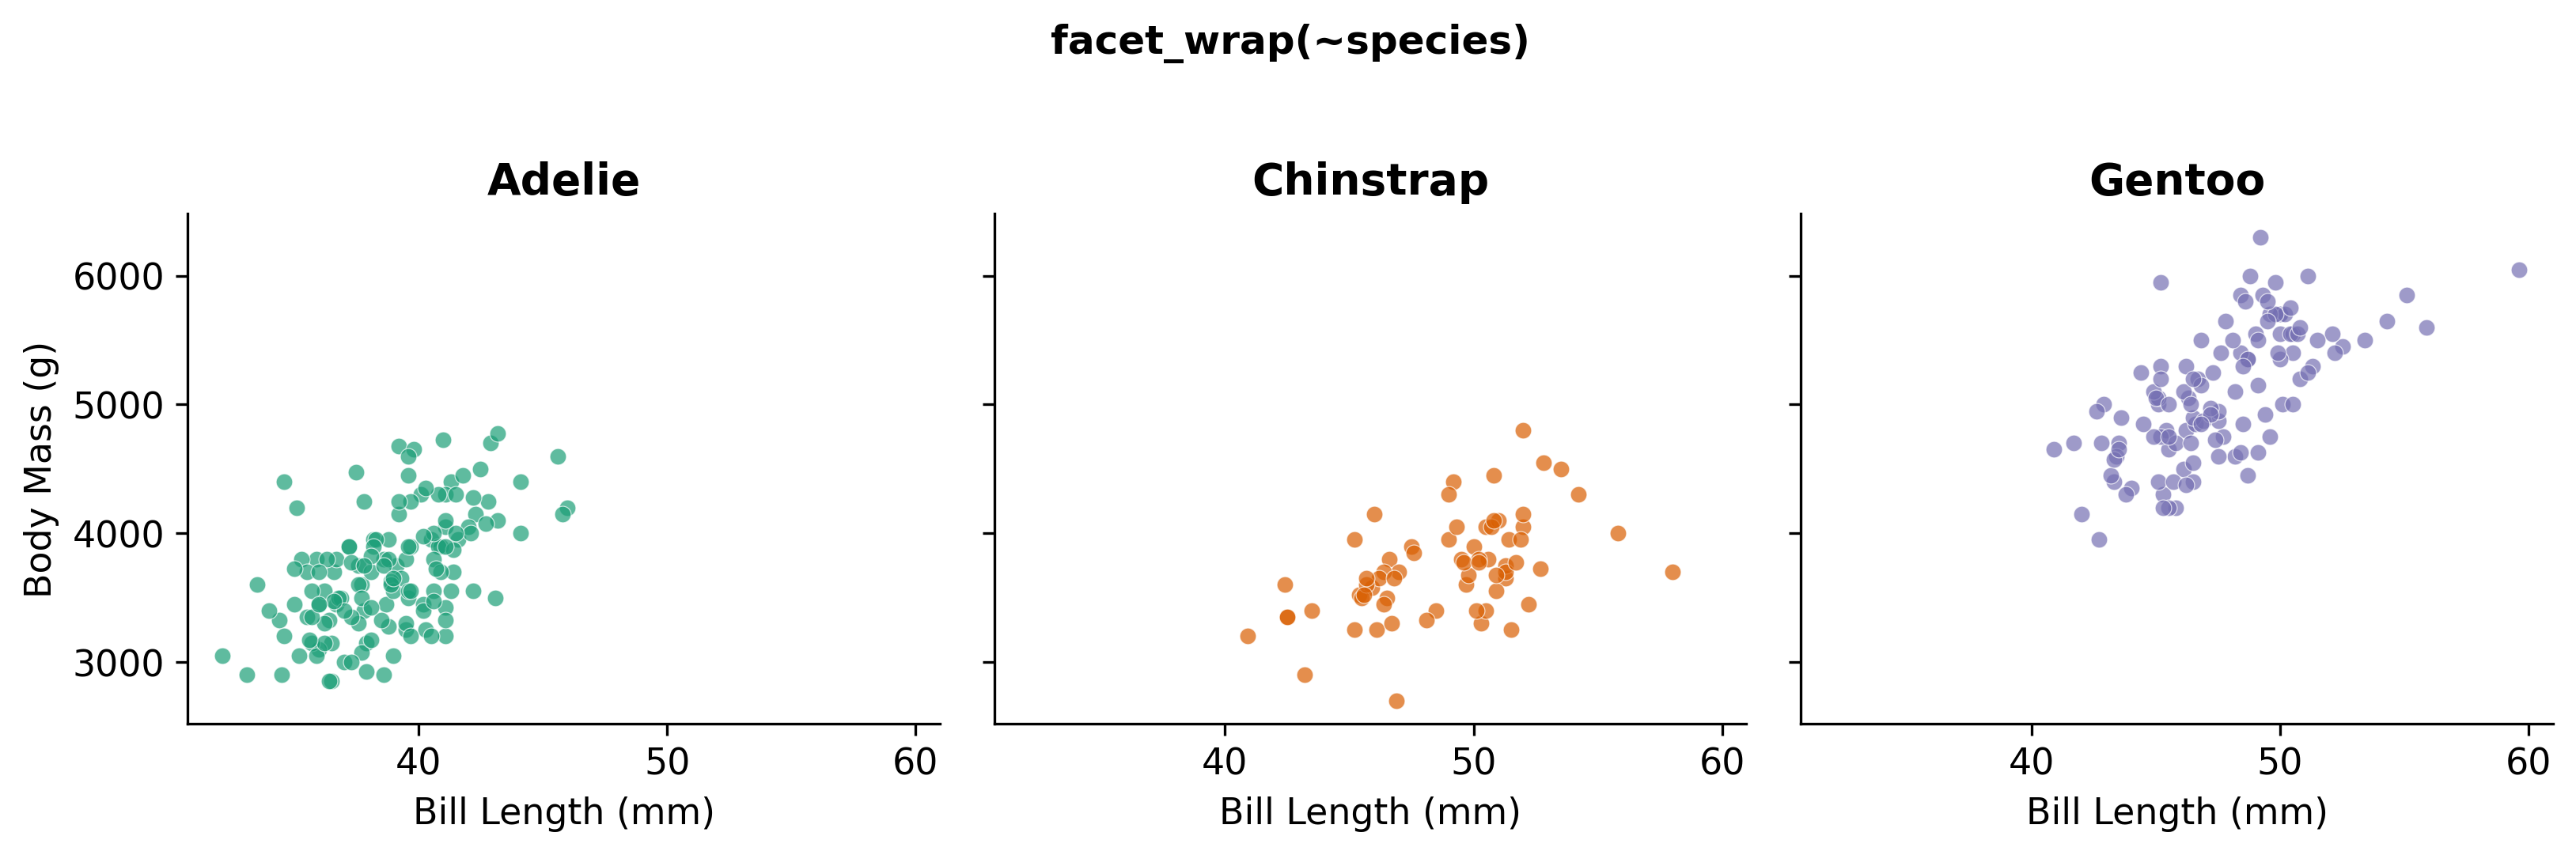
\includegraphics[width=\textwidth]{m1_6_wrap_species.png}
\begin{alertblock}{Pro-Tip}
    \scriptsize In plotnine the formula is a \textbf{string}: \texttt{"$\sim$species"}. In R it is a bare formula: \texttt{$\sim$species}. Common cross-language slip.
\end{alertblock}
\end{column}
\end{columns}
\end{frame}

% ── 156 ──
\begin{frame}{Facet + Color: Two Variables at Once}
\smark{156/300}
\centering
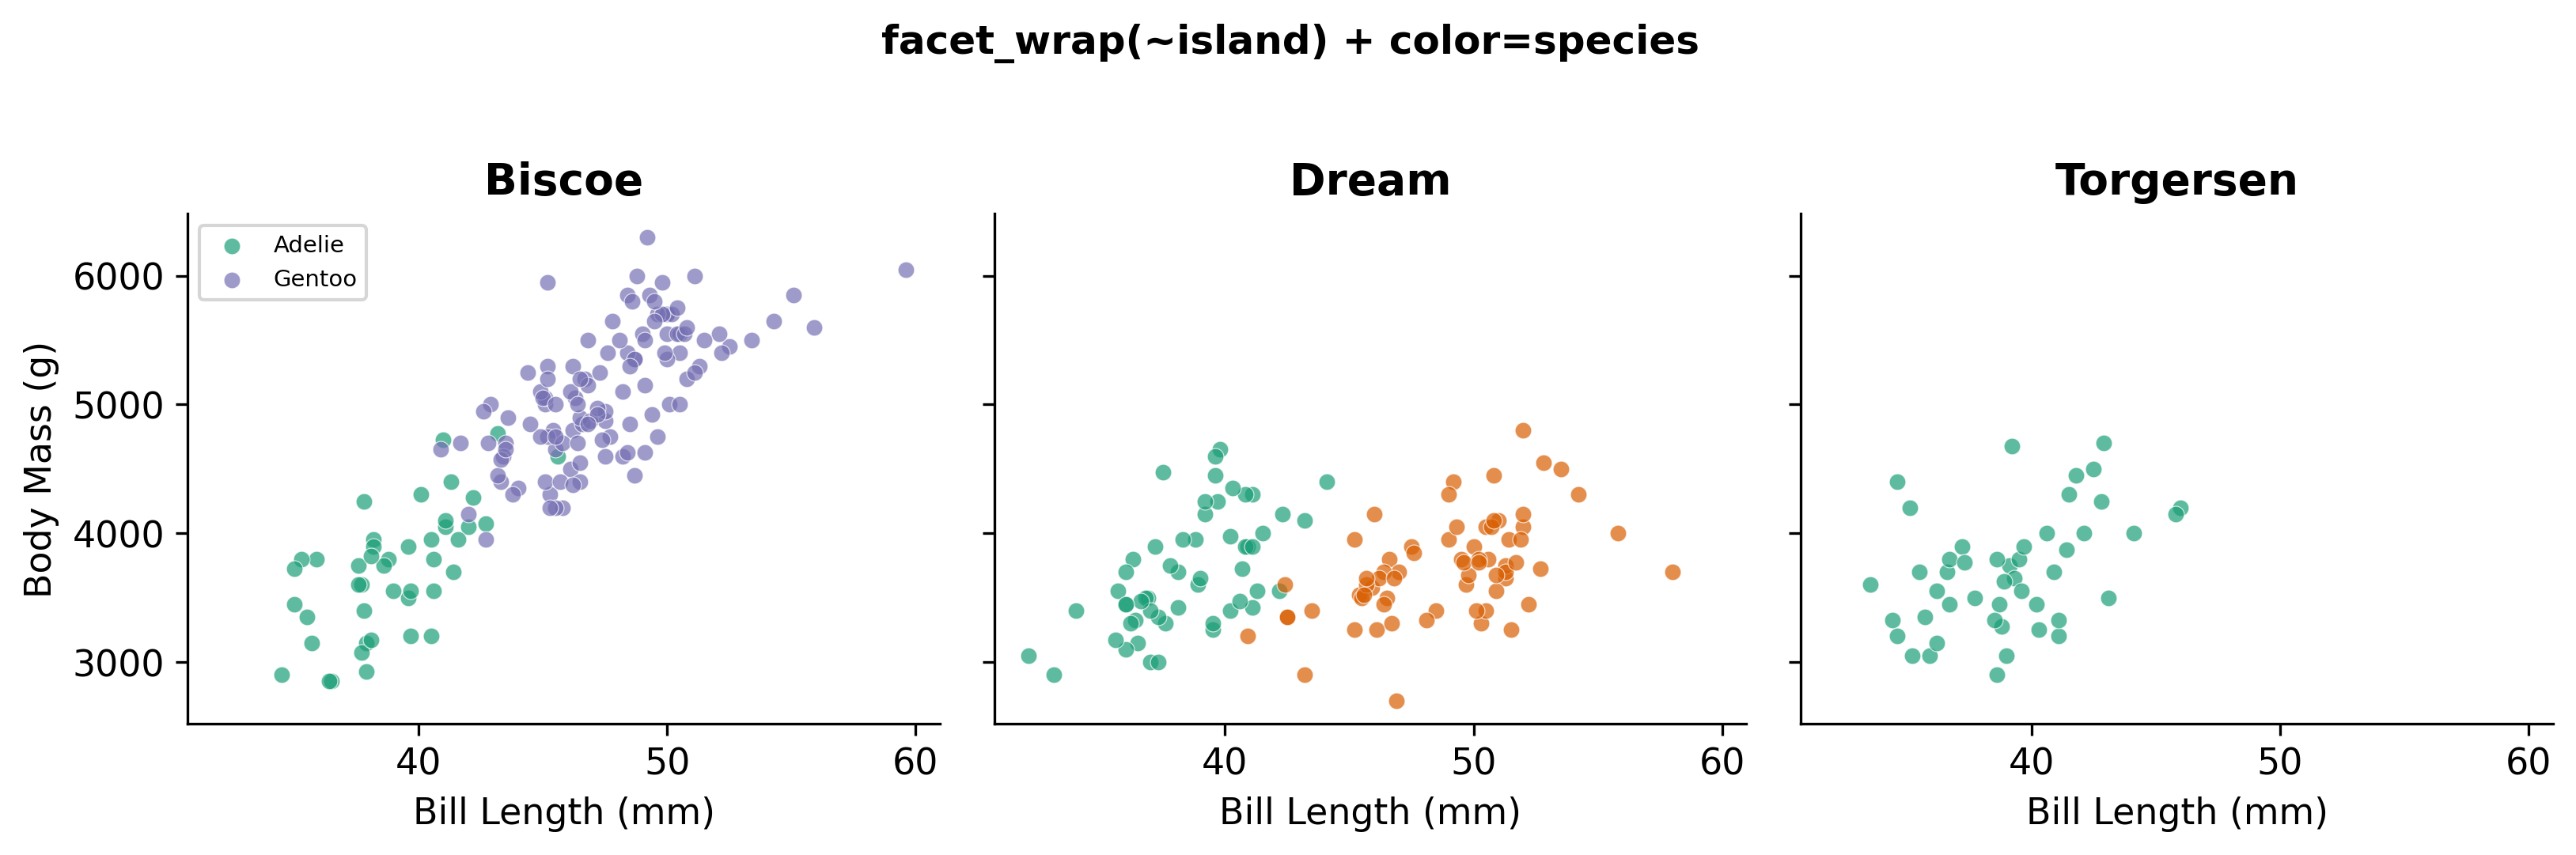
\includegraphics[width=0.85\textwidth]{m1_6_wrap_island.png}

\vspace{0.2cm}
\begin{exampleblock}{Data Insight}
    \scriptsize Facet by \texttt{island}, color by \texttt{species}. Two categorical dimensions displayed without any 2D grid --- facets handle one, color handles the other.
\end{exampleblock}
\end{frame}

% ── 157 ──
\begin{frame}[fragile]{Facet + Color --- Code}\smark{157/300}
\begin{columns}[T]
\begin{column}{0.48\textwidth}
\begin{lstlisting}[style=Rstyle]
ggplot(penguins,
  aes(bill_length_mm,
      body_mass_g,
      color = species)) +
  geom_point(alpha = 0.7) +
  facet_wrap(~island) +
  scale_color_manual(
    values=c("#1B9E77",
             "#D95F02",
             "#7570B3")) +
  theme_minimal()
\end{lstlisting}
\end{column}
\begin{column}{0.48\textwidth}
\begin{lstlisting}[style=Pystyle]
(ggplot(penguins,
   aes("bill_length_mm",
       "body_mass_g",
       color="species"))
 + geom_point(alpha=0.7)
 + facet_wrap("~island")
 + scale_color_manual(
     values=["#1B9E77",
             "#D95F02",
             "#7570B3"]))
\end{lstlisting}
\end{column}
\end{columns}
\end{frame}

% ── 158 ──
\begin{frame}{\texttt{facet\_grid}: Two Variables, 2D Matrix}
\smark{158/300}
\begin{columns}[T]
\begin{column}{0.48\textwidth}
\begin{itemize}
    \item \texttt{facet\_grid(row \textasciitilde\ col)}
    \item Creates a \textbf{matrix} of panels
    \item Rows conditioned on one variable, columns on another
    \item Empty cells appear where combinations have no data
\end{itemize}
\end{column}
\begin{column}{0.49\textwidth}
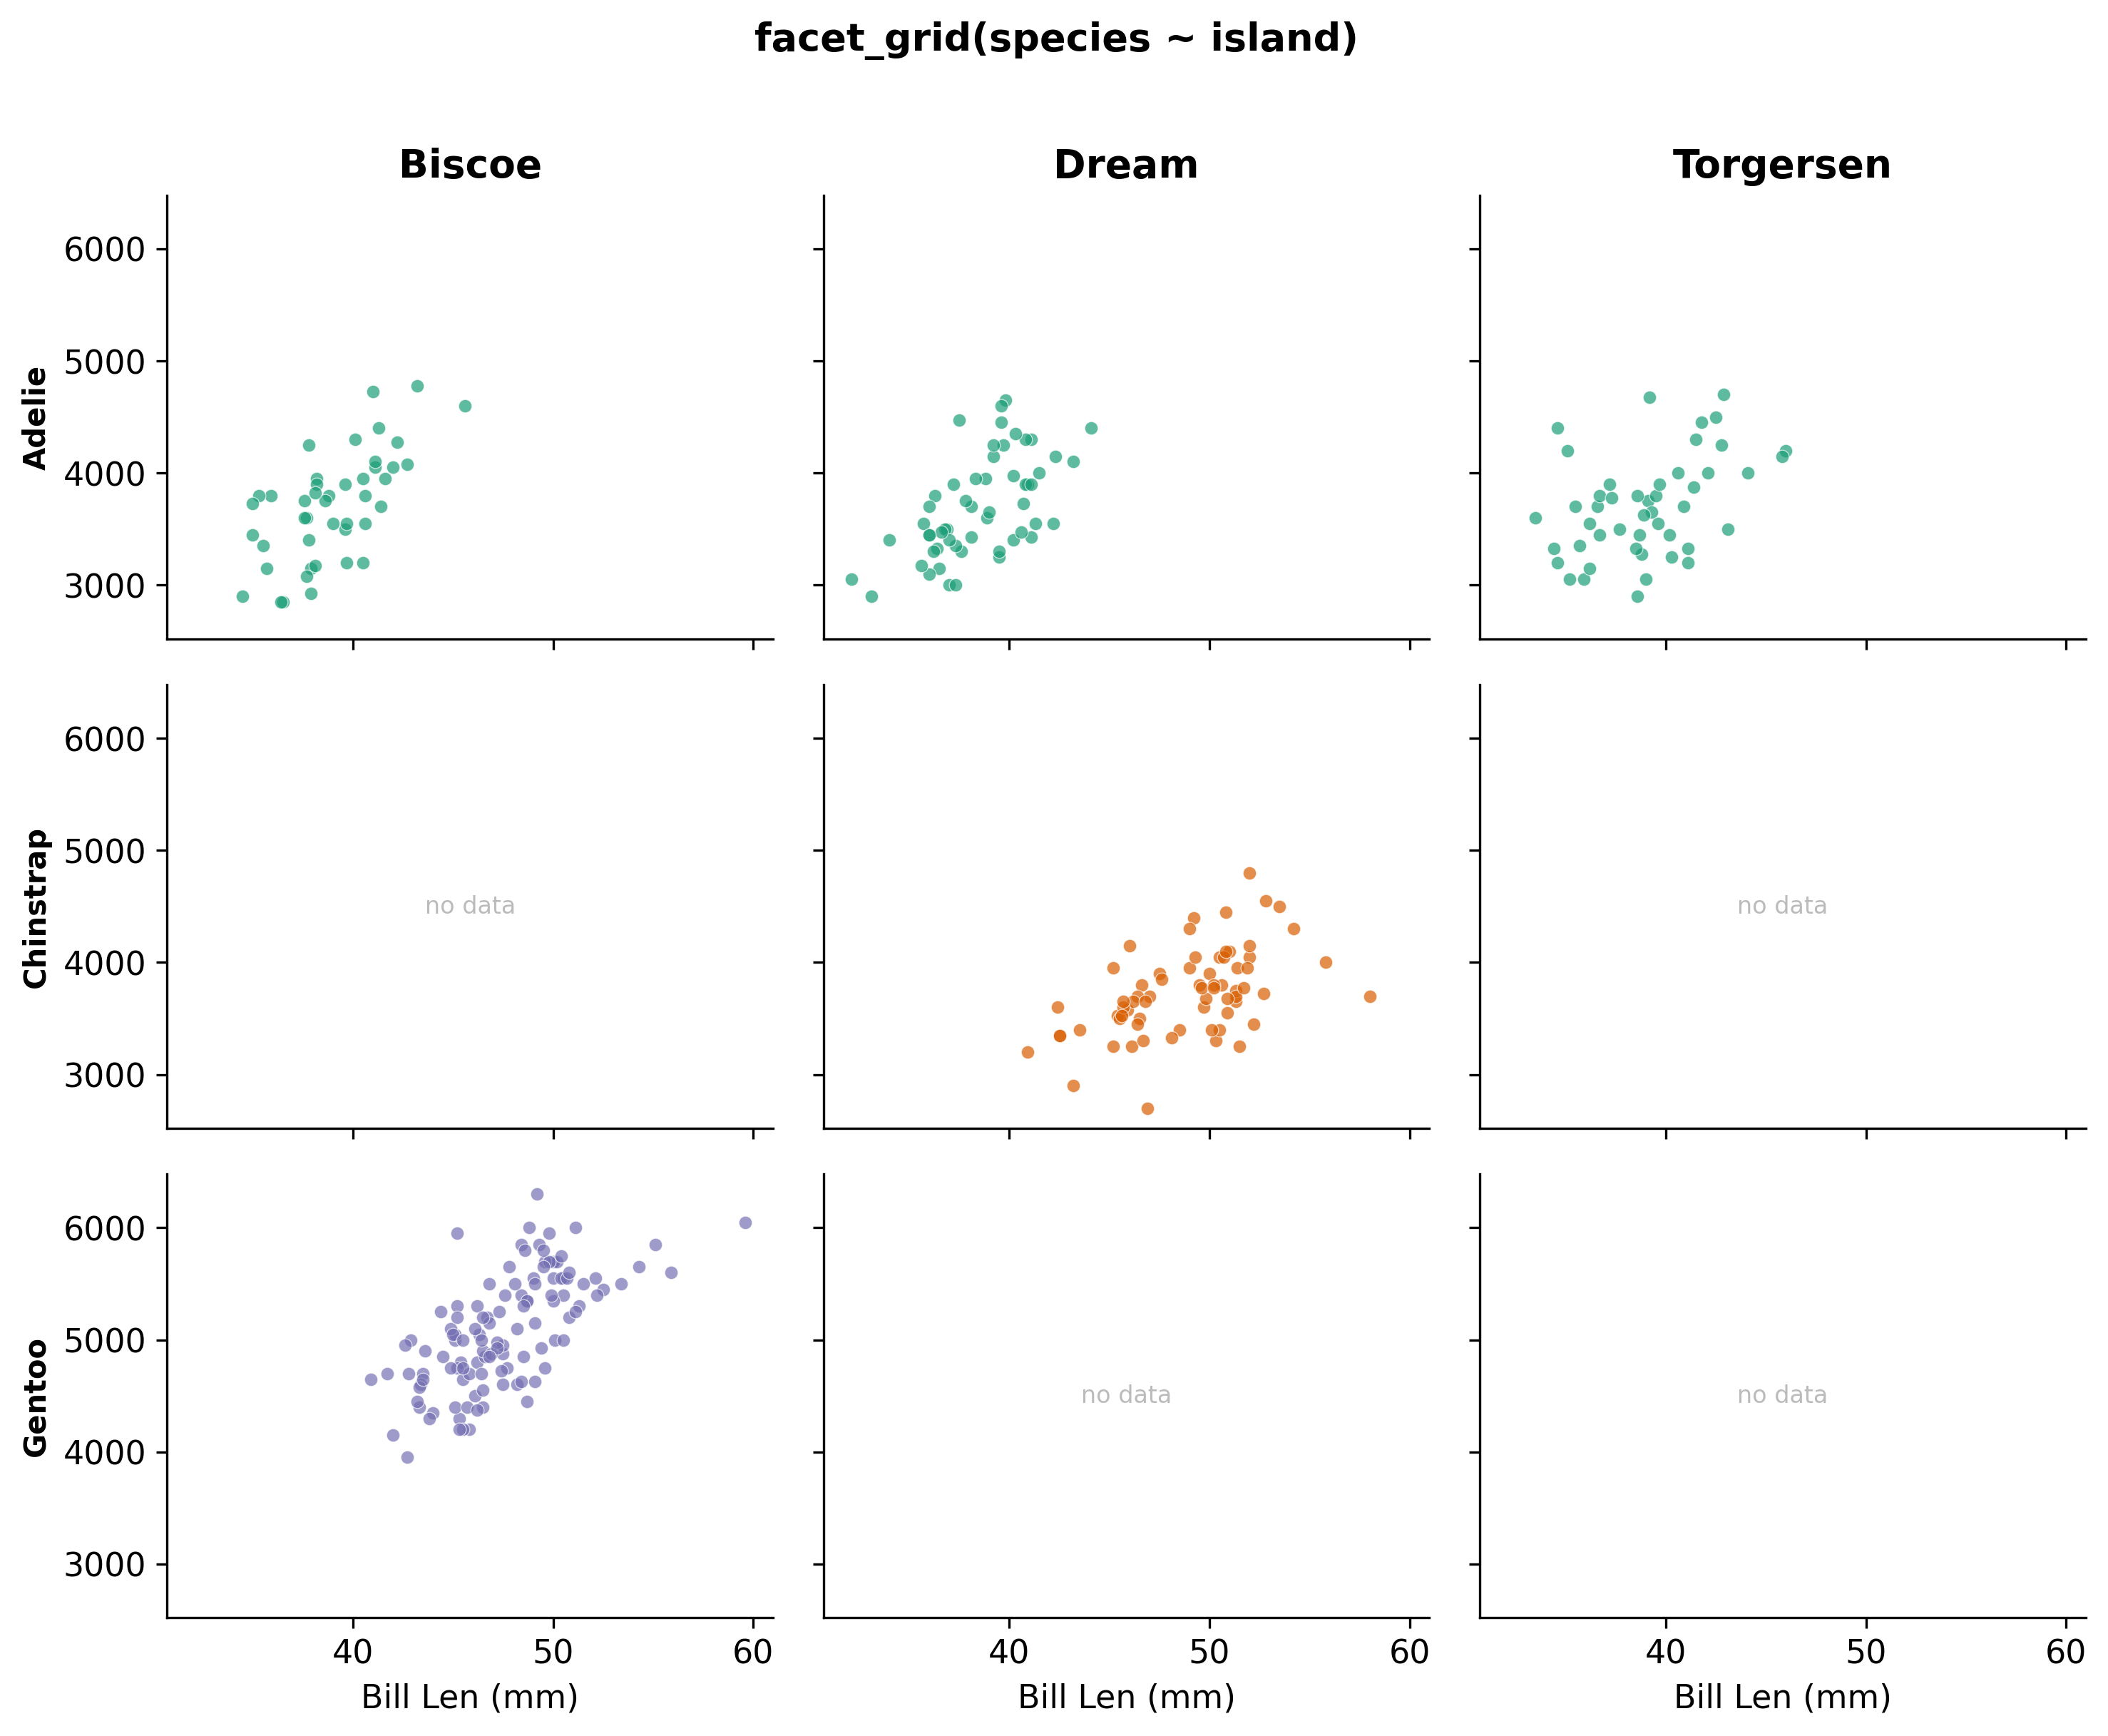
\includegraphics[width=\textwidth]{m1_6_grid.png}
\end{column}
\end{columns}
\end{frame}

% ── 159 ──
\begin{frame}[fragile]{\texttt{facet\_grid} --- \Rlang}\smark{159/300}
\begin{columns}[T]
\begin{column}{0.55\textwidth}
\begin{lstlisting}[style=Rstyle]
ggplot(penguins,
  aes(bill_length_mm,
      body_mass_g)) +
  geom_point(aes(color=species),
             alpha=0.7, size=1.5)+
  facet_grid(species ~ island) +
  theme_minimal() +
  theme(legend.position = "none")
# Rows = species, Cols = island
\end{lstlisting}
\end{column}
\begin{column}{0.42\textwidth}
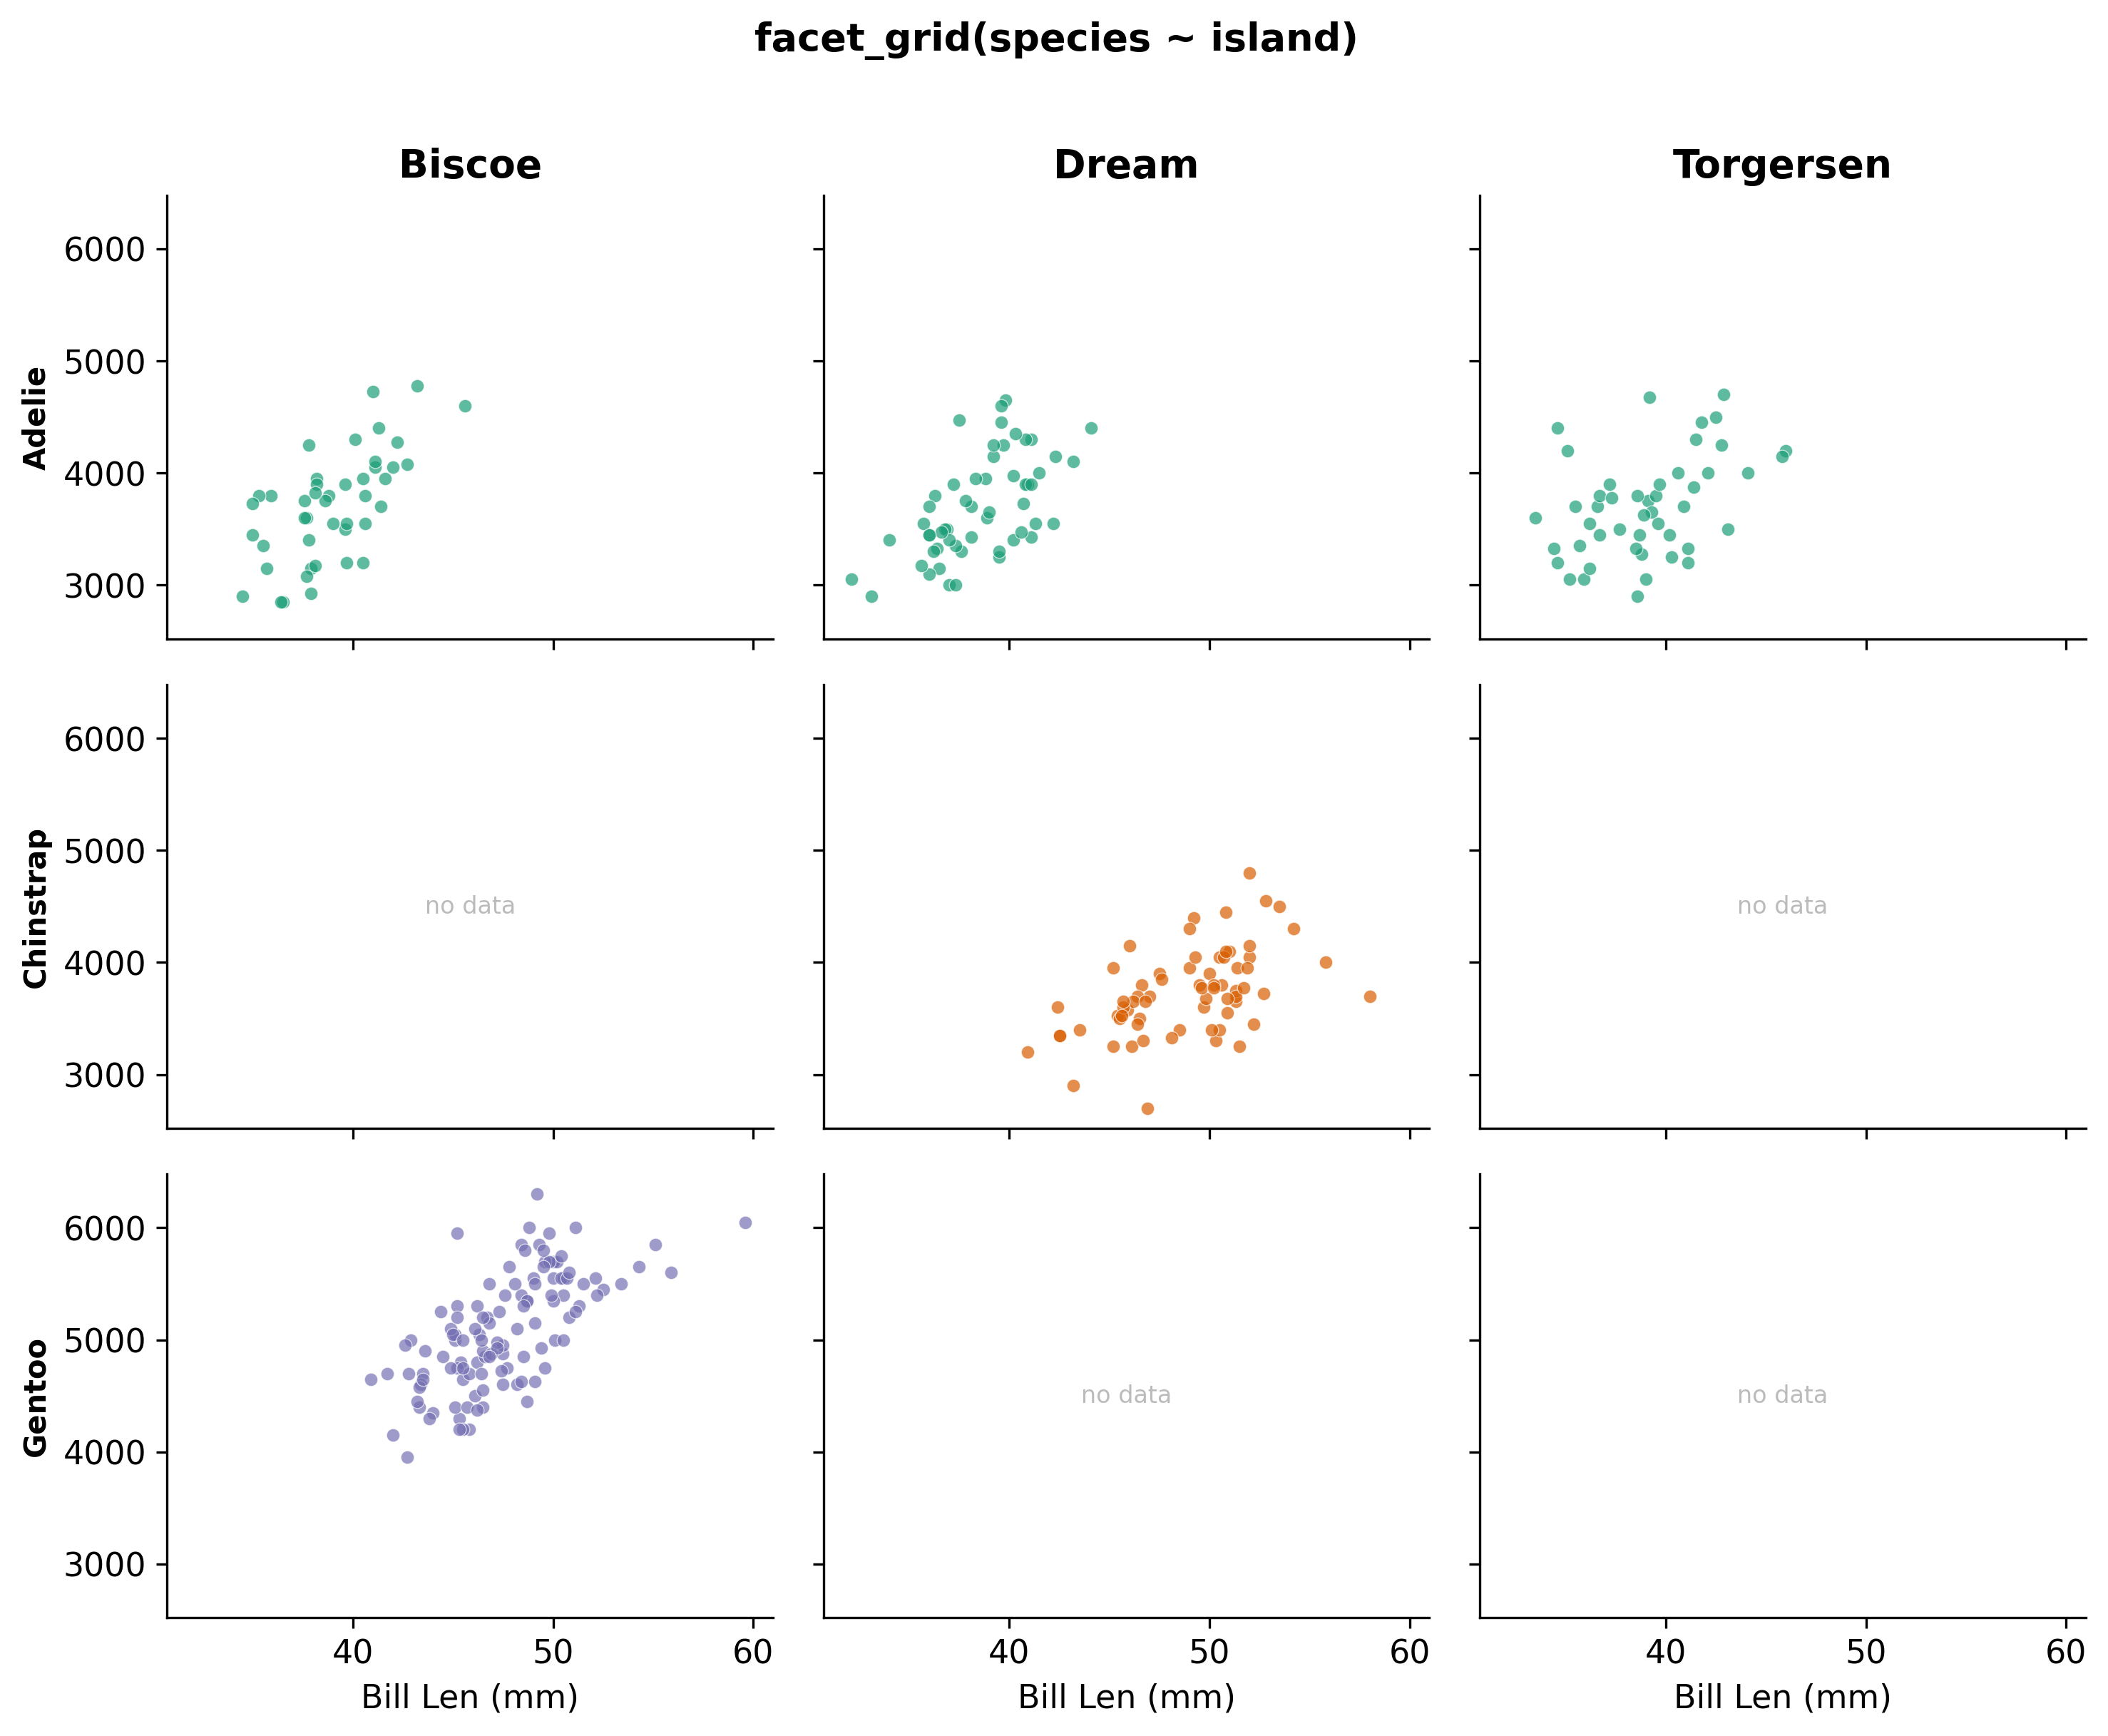
\includegraphics[width=\textwidth]{m1_6_grid.png}
\begin{alertblock}{Pro-Tip}
    \scriptsize Use \texttt{facet\_grid()} when both row and column variables are meaningful. Use \texttt{facet\_wrap()} when you just want to split by one variable.
\end{alertblock}
\end{column}
\end{columns}
\end{frame}

% ── 160 ──
\begin{frame}[fragile]{\texttt{facet\_grid} --- \Python}\smark{160/300}
\begin{columns}[T]
\begin{column}{0.55\textwidth}
\begin{lstlisting}[style=Pystyle]
# plotnine
(ggplot(penguins,
   aes("bill_length_mm",
       "body_mass_g",
       color="species"))
 + geom_point(alpha=0.7, size=1.5)
 + facet_grid("species~island")
 + theme_minimal()
 + theme(legend_position="none"))

# seaborn
g = sns.FacetGrid(penguins,
    row="species", col="island",
    height=2.5)
g.map_dataframe(sns.scatterplot,
    x="bill_length_mm",
    y="body_mass_g", alpha=0.7)
\end{lstlisting}
\end{column}
\begin{column}{0.42\textwidth}
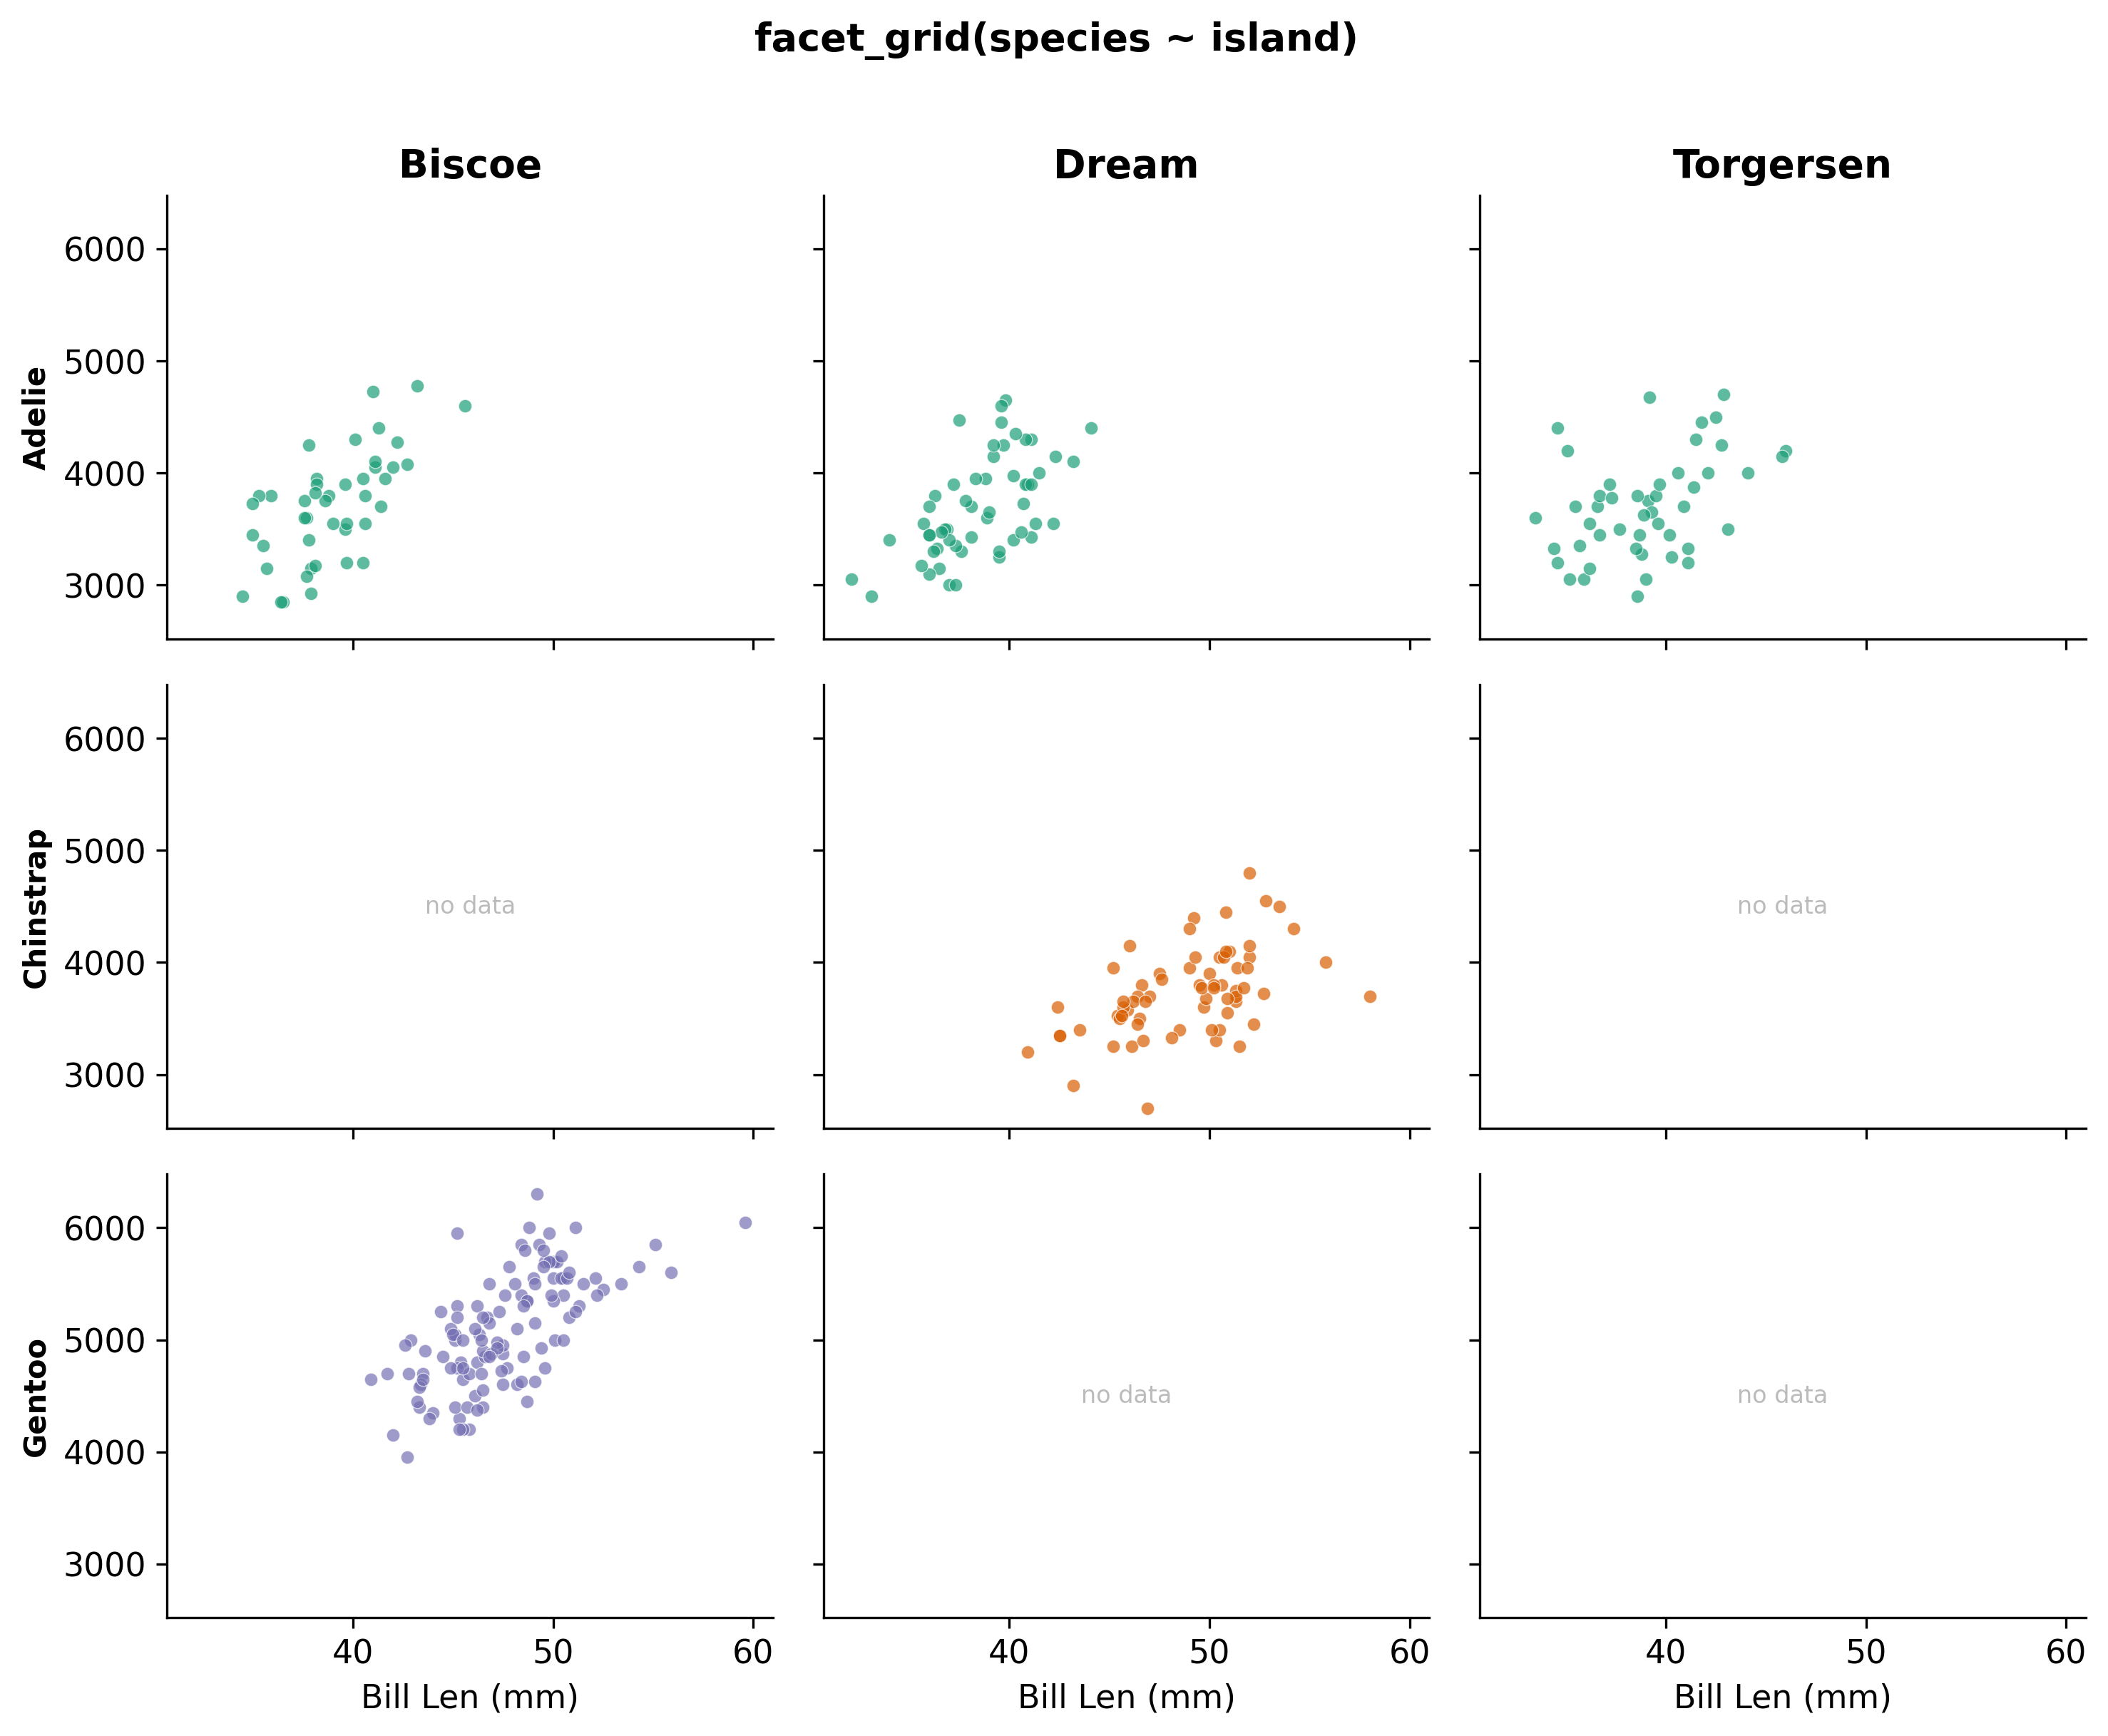
\includegraphics[width=\textwidth]{m1_6_grid.png}
\begin{exampleblock}{Data Insight}
    \scriptsize Empty panels (e.g., Chinstrap/Biscoe) are informative --- they show that combination does not exist in the data.
\end{exampleblock}
\end{column}
\end{columns}
\end{frame}

% ── 161 ──
\begin{frame}{Free vs.\ Fixed Scales}
\smark{161/300}
\centering
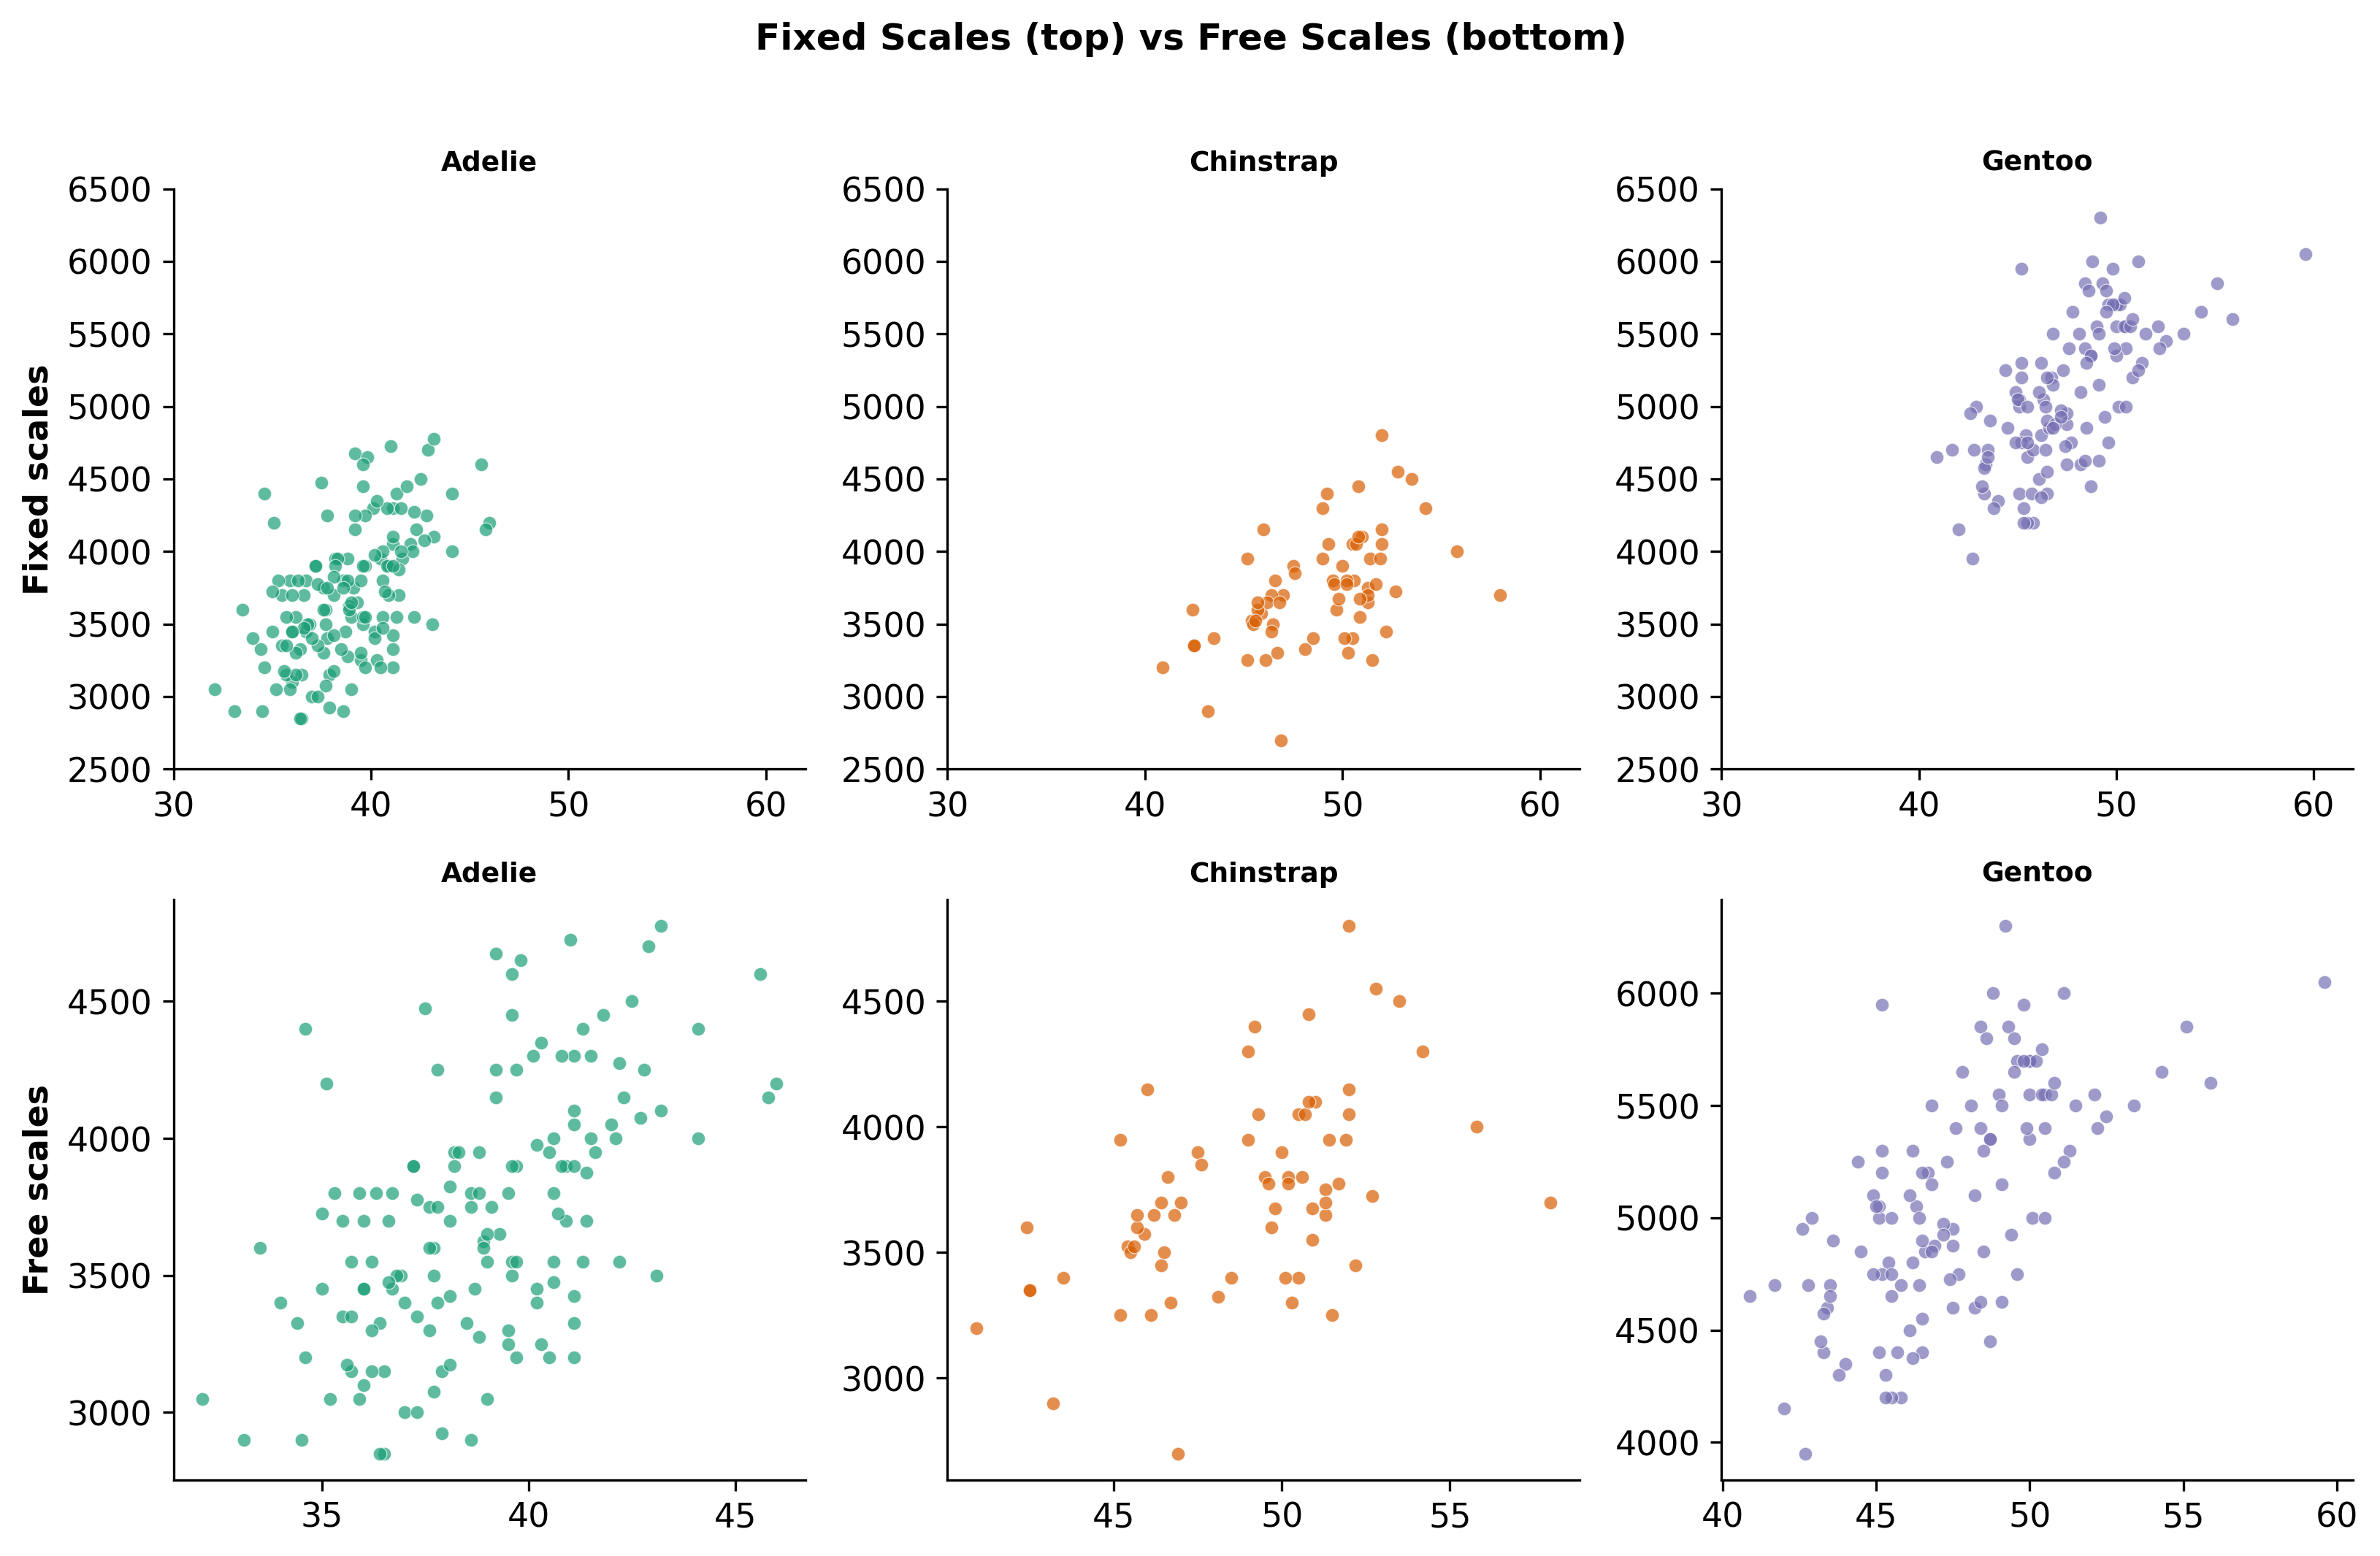
\includegraphics[width=0.85\textwidth]{m1_6_free_vs_fixed.png}

\vspace{0.2cm}
\begin{columns}[T]
\begin{column}{0.48\textwidth}
\begin{exampleblock}{Data Insight}
    \scriptsize \textbf{Fixed} (top): position comparisons across panels are valid. Gentoo is visibly heavier. \textbf{Free} (bottom): each panel uses its full range, revealing within-group detail but making cross-panel comparison invalid.
\end{exampleblock}
\end{column}
\begin{column}{0.48\textwidth}
\begin{alertblock}{Pro-Tip}
    \scriptsize Default to \textbf{fixed} scales. Use \texttt{scales="free"} only when group ranges differ so dramatically that the smaller group is invisible at the shared scale.
\end{alertblock}
\end{column}
\end{columns}
\end{frame}

% ── 162 ──
\begin{frame}[fragile]{Free Scales --- Code}\smark{162/300}
\begin{columns}[T]
\begin{column}{0.48\textwidth}
\begin{lstlisting}[style=Rstyle]
# Fixed (default)
facet_wrap(~species)

# Free both axes
facet_wrap(~species,
           scales = "free")

# Free y only
facet_wrap(~species,
           scales = "free_y")

# Free x only
facet_wrap(~species,
           scales = "free_x")
\end{lstlisting}
\end{column}
\begin{column}{0.48\textwidth}
\begin{lstlisting}[style=Pystyle]
# plotnine: same syntax
facet_wrap("~species",
           scales="free")

# seaborn FacetGrid
g = sns.FacetGrid(penguins,
    col="species",
    sharey=False,  # free y
    sharex=True)   # fixed x
\end{lstlisting}
\vspace{0.2cm}
\begin{alertblock}{Pro-Tip}
    \scriptsize seaborn uses \texttt{sharex/sharey} booleans. plotnine uses the ggplot2 \texttt{scales=} string.
\end{alertblock}
\end{column}
\end{columns}
\end{frame}

% ── 163 ──
\begin{frame}{Controlling Layout: \texttt{ncol}, \texttt{nrow}, Panel Order}
\smark{163/300}
\begin{columns}[T]
\begin{column}{0.50\textwidth}
\begin{itemize}
    \item \texttt{ncol=2} forces 2 columns (panels wrap into rows)
    \item \texttt{nrow=1} forces a single horizontal strip
    \item Panel \textbf{order} follows factor levels
    \item Reorder with \texttt{forcats::fct\_relevel()} in R or \texttt{pd.Categorical(ordered=True)} in Python
\end{itemize}
\end{column}
\begin{column}{0.47\textwidth}
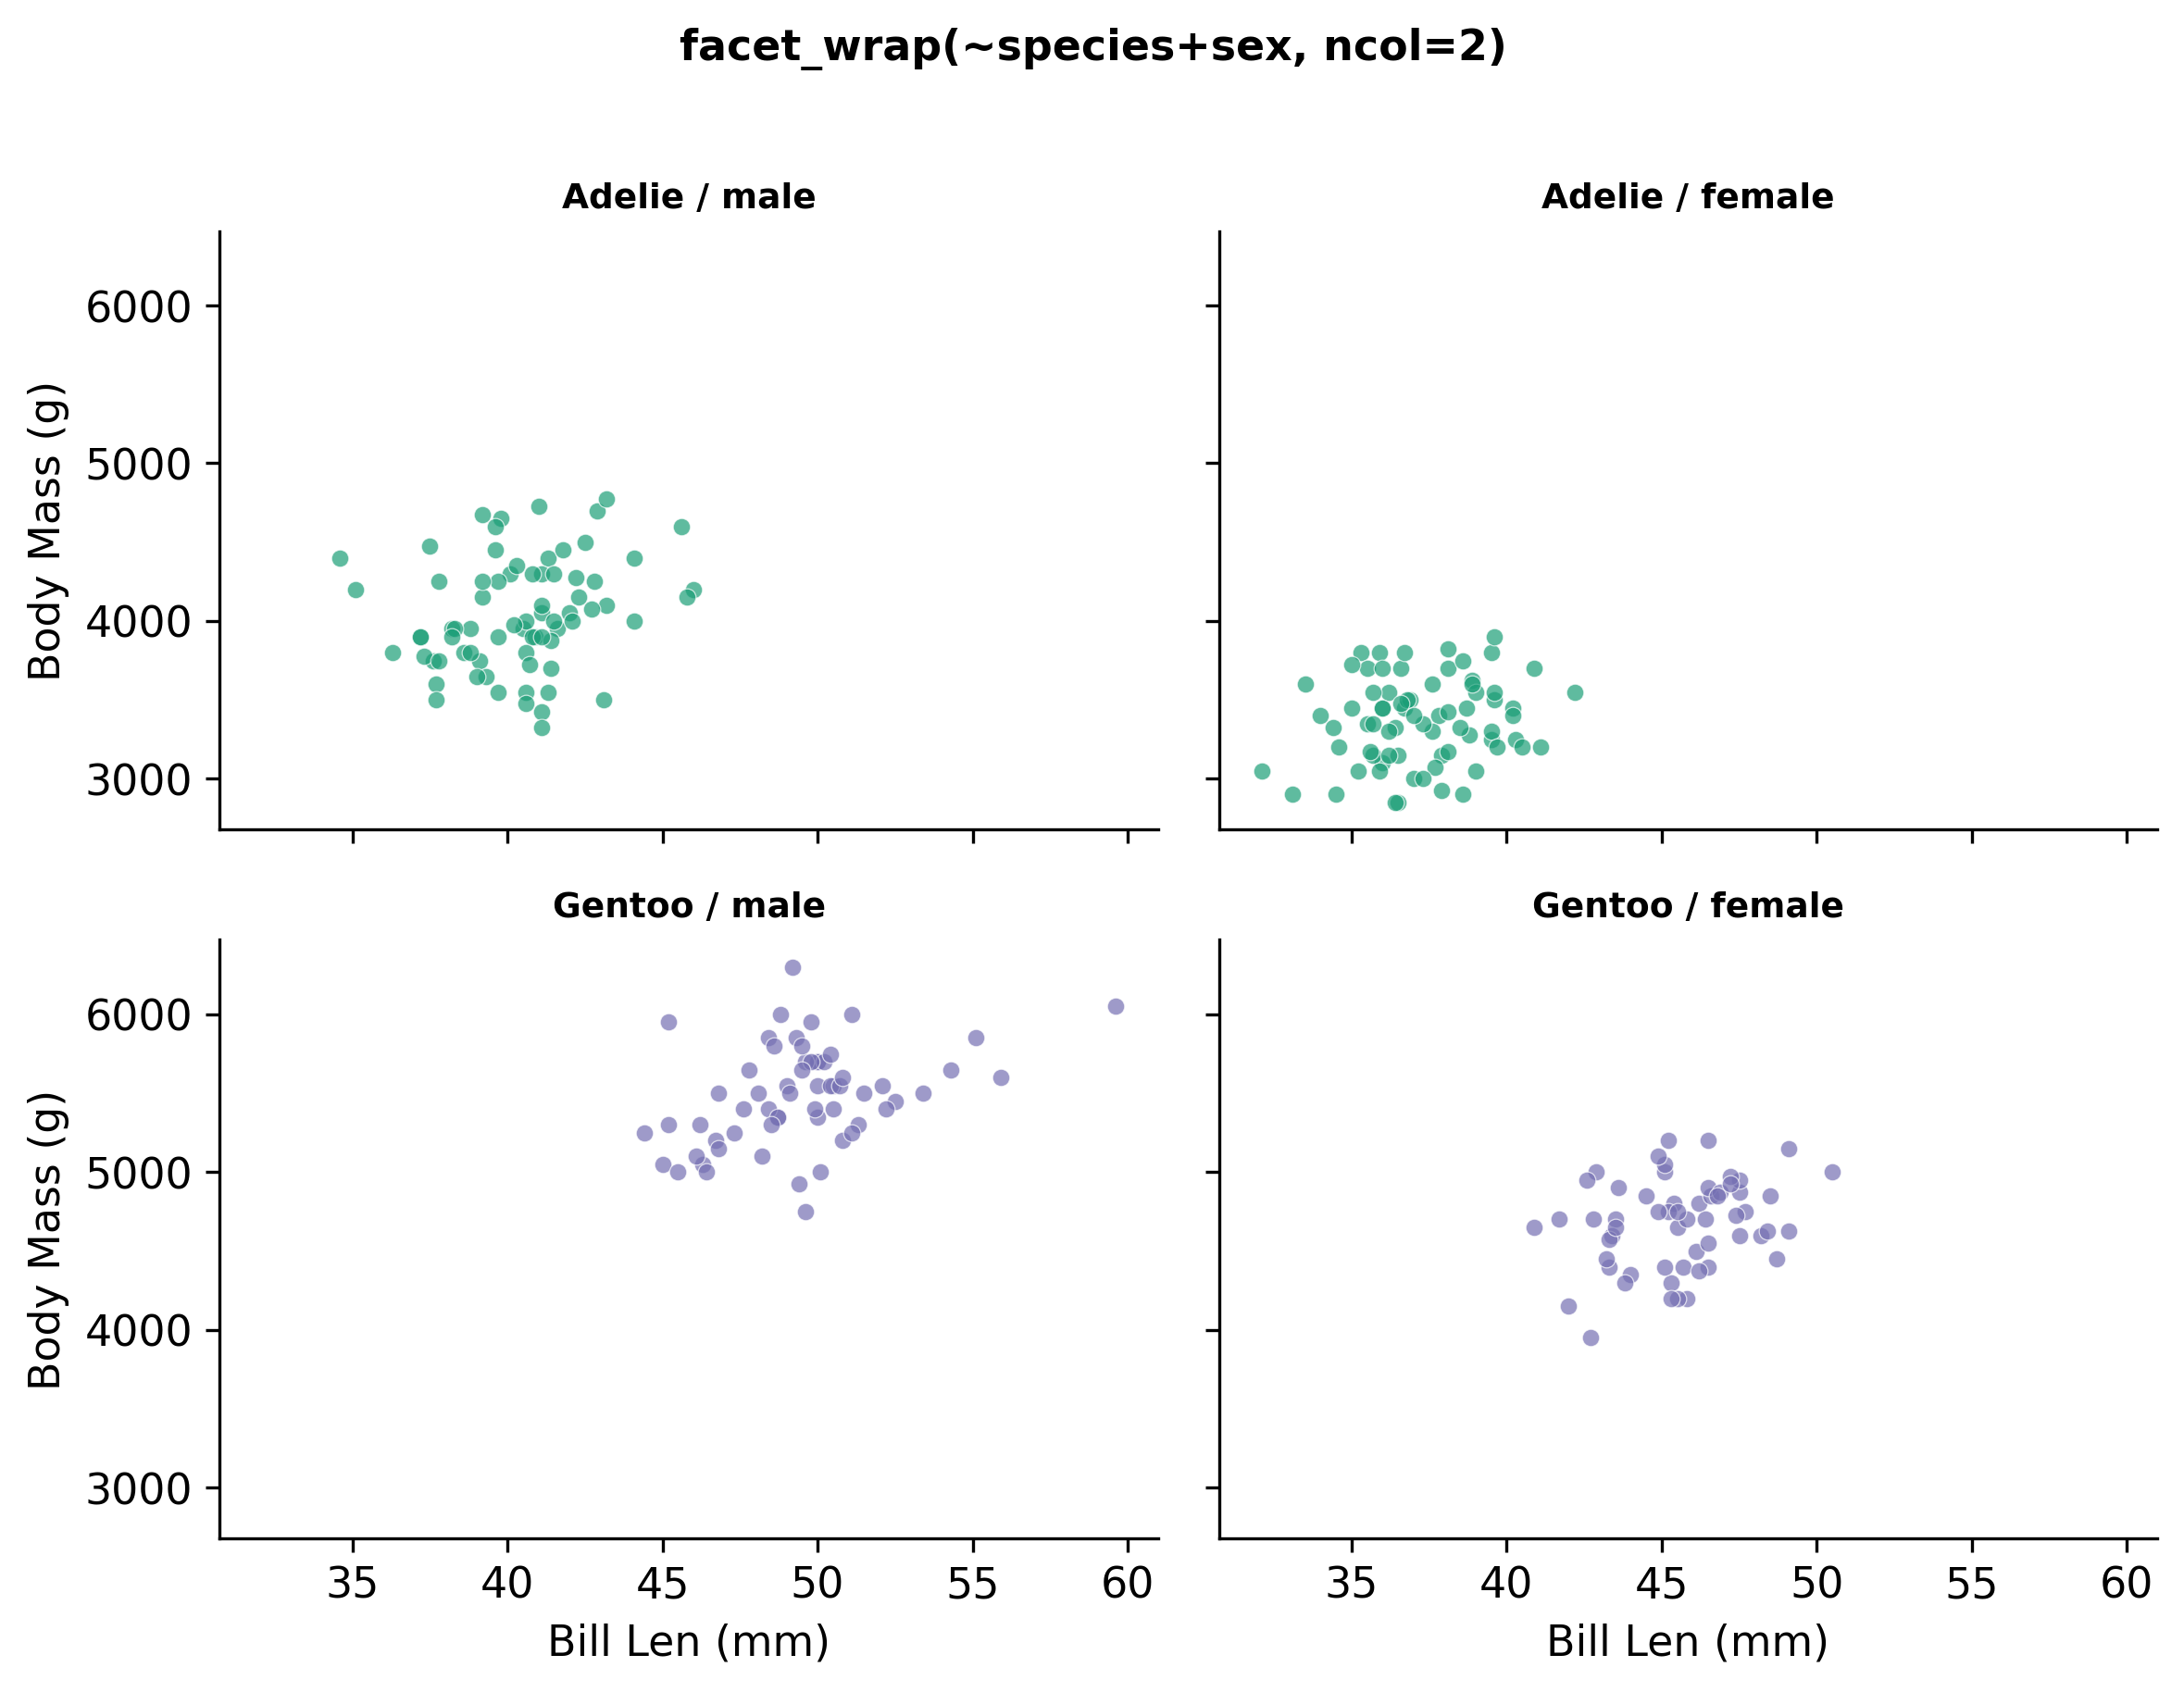
\includegraphics[width=\textwidth]{m1_6_wrap_ncol.png}
\begin{exampleblock}{Data Insight}
    \scriptsize 4 panels from 2 variables (species $\times$ sex) arranged in a 2$\times$2 grid via \texttt{ncol=2}. Faceting on \textbf{interaction terms} is powerful.
\end{exampleblock}
\end{column}
\end{columns}
\end{frame}

% ── 164 ──
\begin{frame}[fragile]{Layout Control --- Code}\smark{164/300}
\begin{columns}[T]
\begin{column}{0.48\textwidth}
\begin{lstlisting}[style=Rstyle]
# 2 columns, rows auto
facet_wrap(~species + sex,
           ncol = 2)

# Reorder panels
penguins |>
  mutate(species =
    fct_relevel(species,
      "Gentoo","Chinstrap",
      "Adelie")) |>
  ggplot(aes(bill_length_mm,
             body_mass_g)) +
  geom_point() +
  facet_wrap(~species)
\end{lstlisting}
\end{column}
\begin{column}{0.48\textwidth}
\begin{lstlisting}[style=Pystyle]
# plotnine
facet_wrap("~species+sex",
           ncol=2)

# Reorder in pandas
pen["species"] = pd.Categorical(
    pen["species"],
    categories=["Gentoo",
                "Chinstrap",
                "Adelie"],
    ordered=True)
\end{lstlisting}
\vspace{0.2cm}
\begin{alertblock}{Pro-Tip}
    \scriptsize Panel order = factor level order. Control the factor \textbf{before} plotting.
\end{alertblock}
\end{column}
\end{columns}
\end{frame}

% ── 165 ──
\begin{frame}{Small Multiples with Context}
\smark{165/300}
\centering
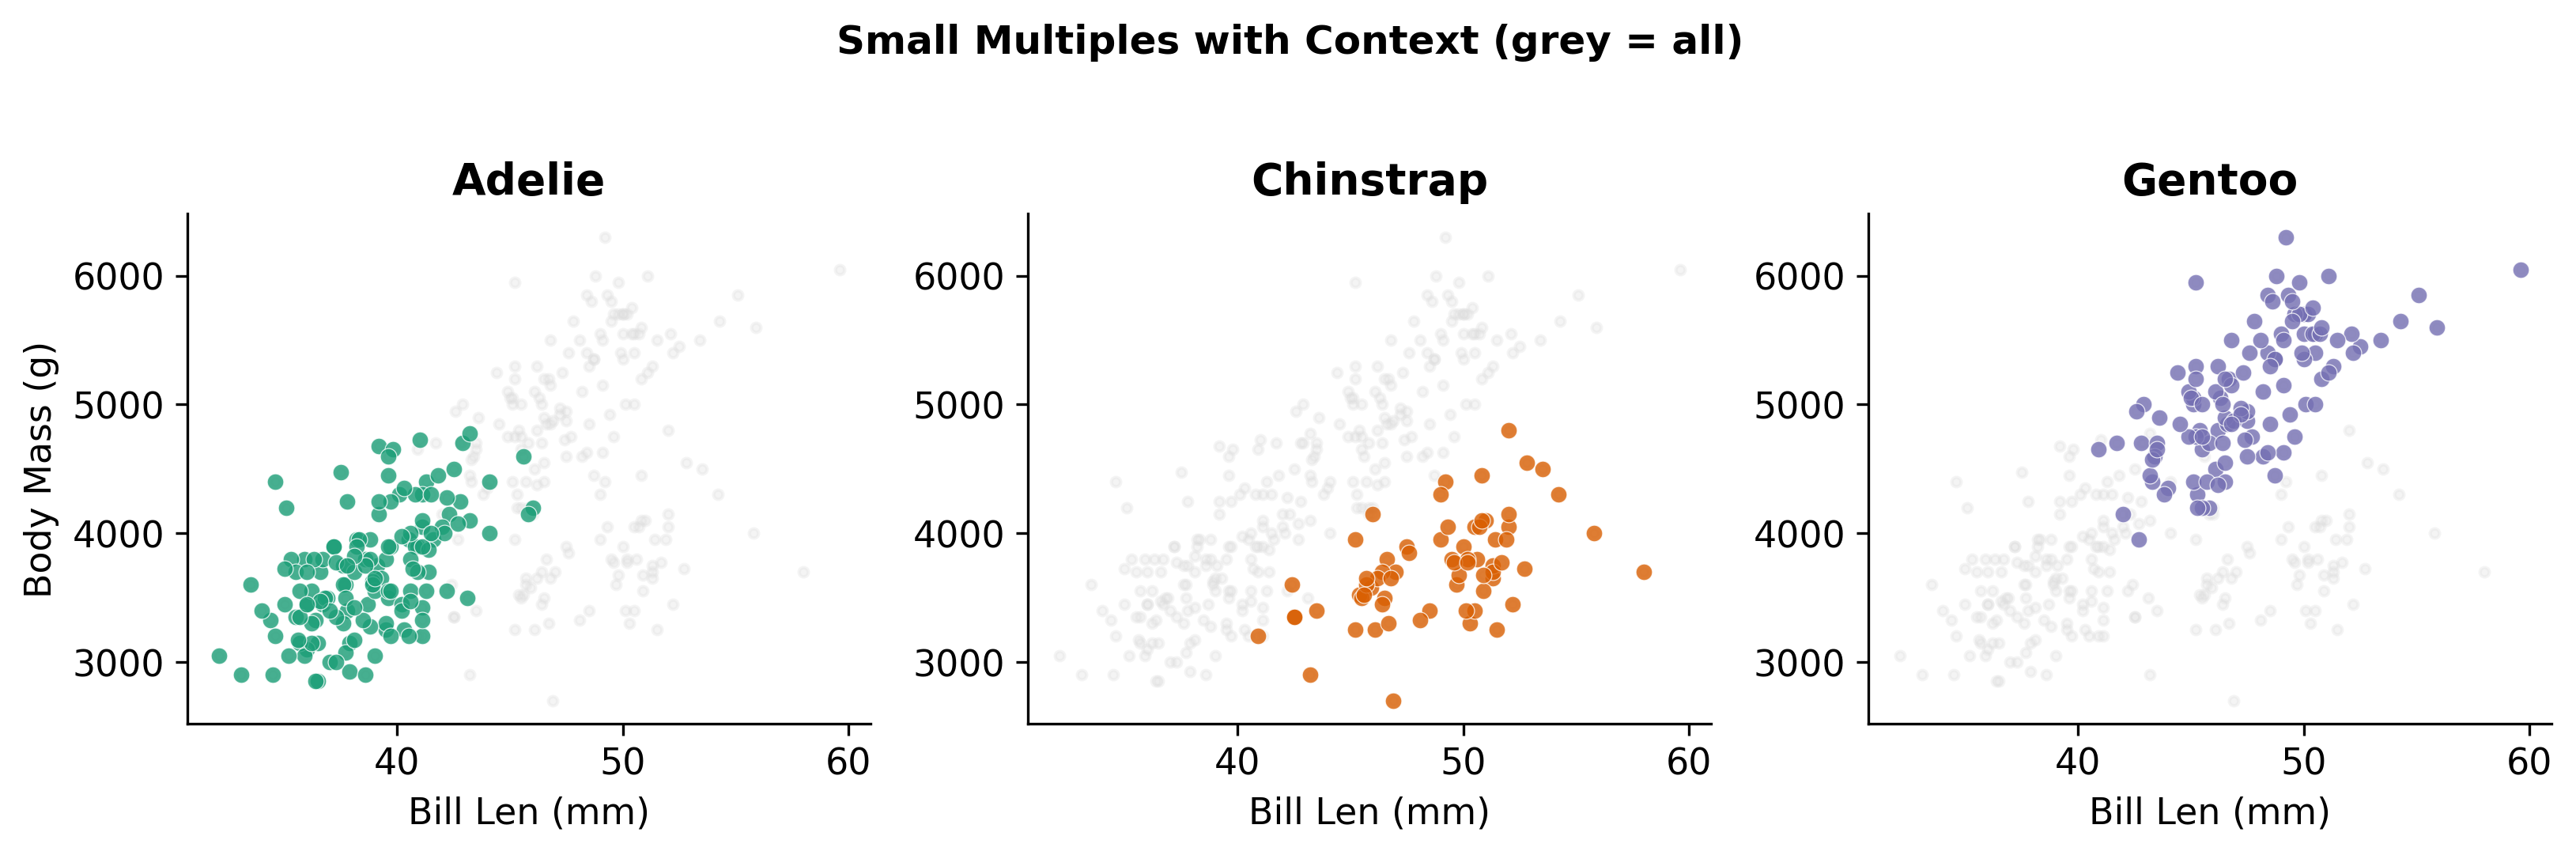
\includegraphics[width=0.88\textwidth]{m1_6_small_multiples_context.png}

\vspace{0.2cm}
\begin{exampleblock}{Data Insight}
    \scriptsize Each panel highlights one species in color against the \textbf{full dataset in grey}. The reader sees both the group's position and its context simultaneously. This is the ``Tufte ideal'' of small multiples.
\end{exampleblock}
\end{frame}

% ── 166 ──
\begin{frame}[fragile]{Context Pattern --- \Rlang}\smark{166/300}
\begin{columns}[T]
\begin{column}{0.55\textwidth}
\begin{lstlisting}[style=Rstyle]
# Grey background = all data
# Colored foreground = facet group
ggplot(penguins,
  aes(bill_length_mm,
      body_mass_g)) +
  # Layer 1: grey context
  geom_point(
    data = penguins |>
      select(-species),
    color = "#DDDDDD",
    size = 0.8, alpha = 0.3) +
  # Layer 2: colored group
  geom_point(aes(color=species),
    size = 2, alpha = 0.8) +
  facet_wrap(~species) +
  theme(legend.position="none")
\end{lstlisting}
\end{column}
\begin{column}{0.42\textwidth}
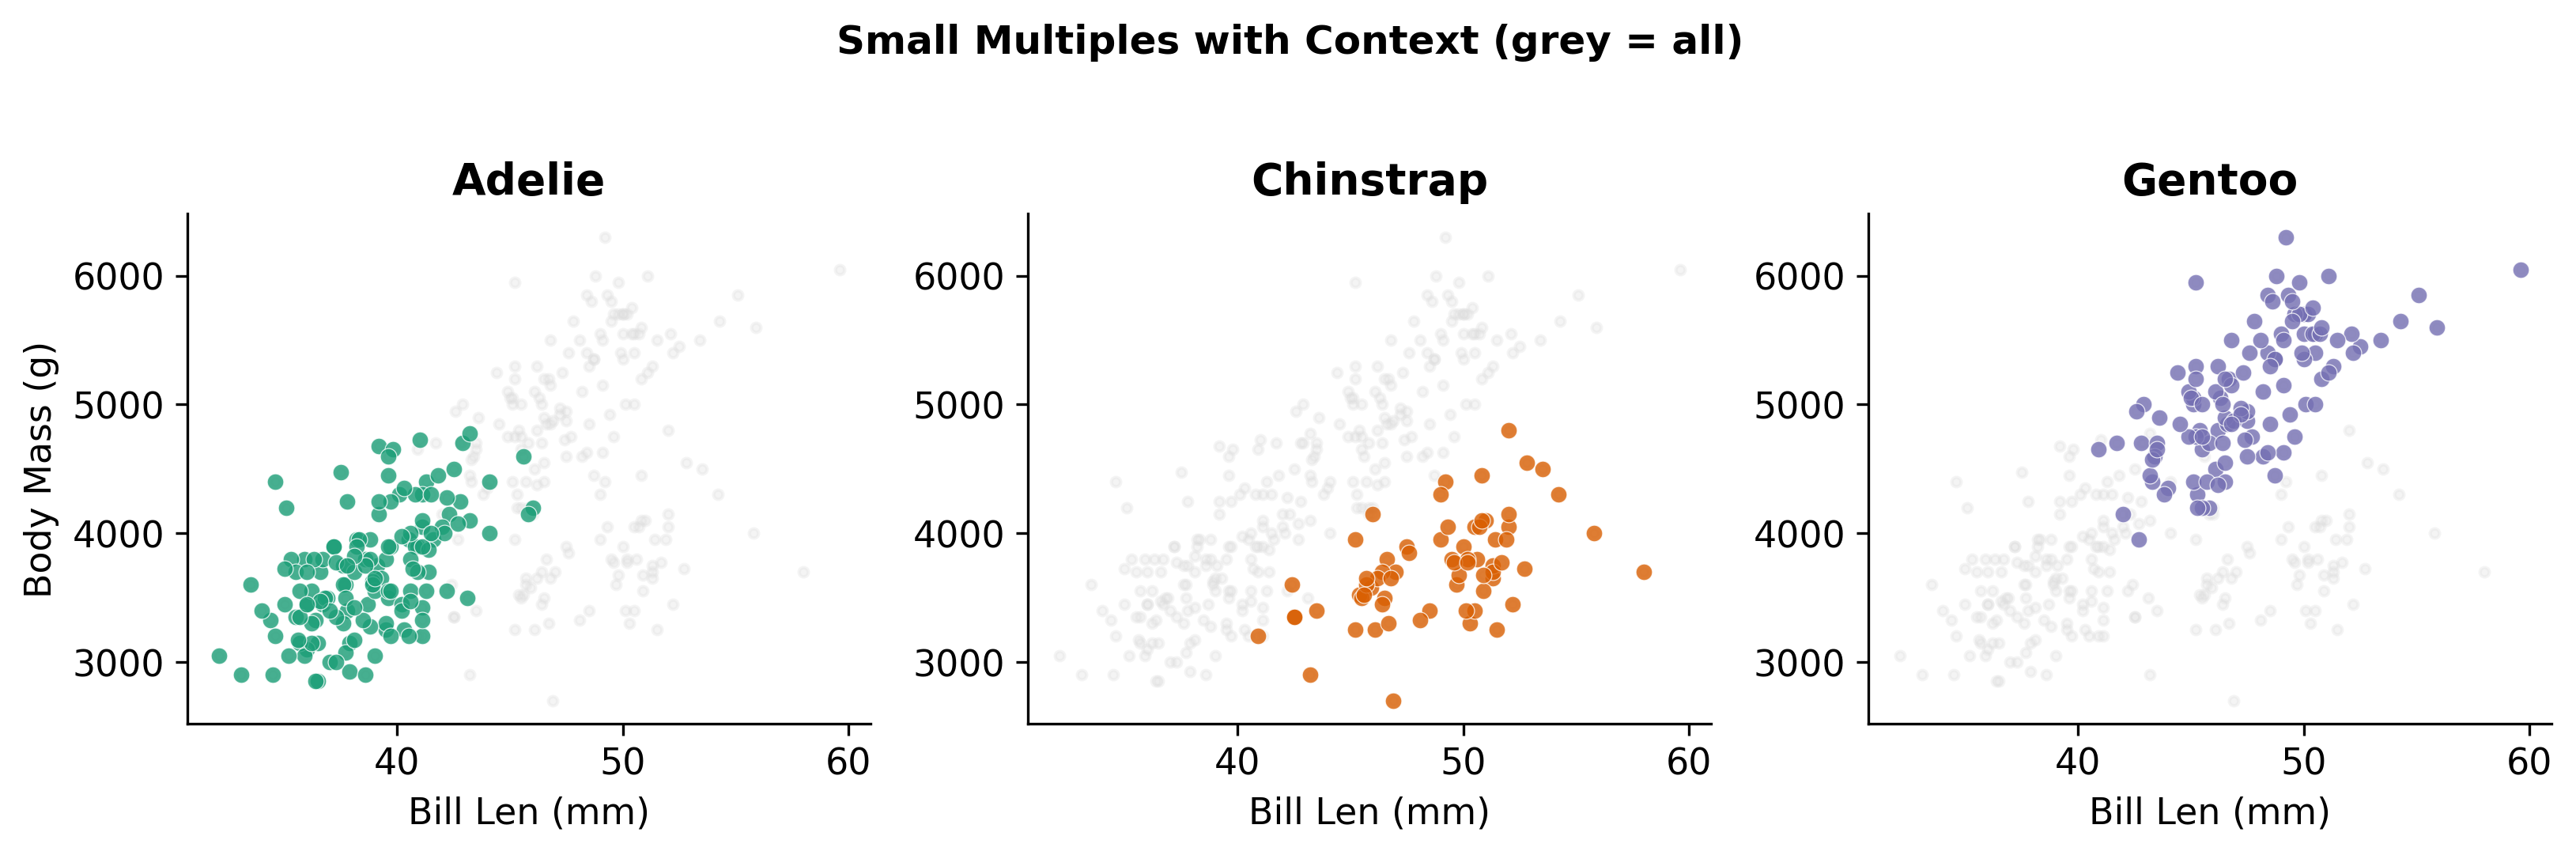
\includegraphics[width=\textwidth]{m1_6_small_multiples_context.png}
\begin{alertblock}{Pro-Tip}
    \scriptsize The trick: pass a data frame \textbf{without the facet variable} to the grey layer. It then draws in every panel.
\end{alertblock}
\end{column}
\end{columns}
\end{frame}

% ── 167 ──
\begin{frame}[fragile]{Context Pattern --- \Python}\smark{167/300}
\begin{columns}[T]
\begin{column}{0.55\textwidth}
\begin{lstlisting}[style=Pystyle]
# plotnine: same trick
bg = penguins.drop(
    columns="species")

(ggplot(penguins,
   aes("bill_length_mm",
       "body_mass_g"))
 + geom_point(data=bg,
     color="#DDDDDD",
     size=0.8, alpha=0.3)
 + geom_point(aes(color="species"),
     size=2, alpha=0.8)
 + facet_wrap("~species")
 + theme(legend_position="none"))
\end{lstlisting}
\end{column}
\begin{column}{0.42\textwidth}
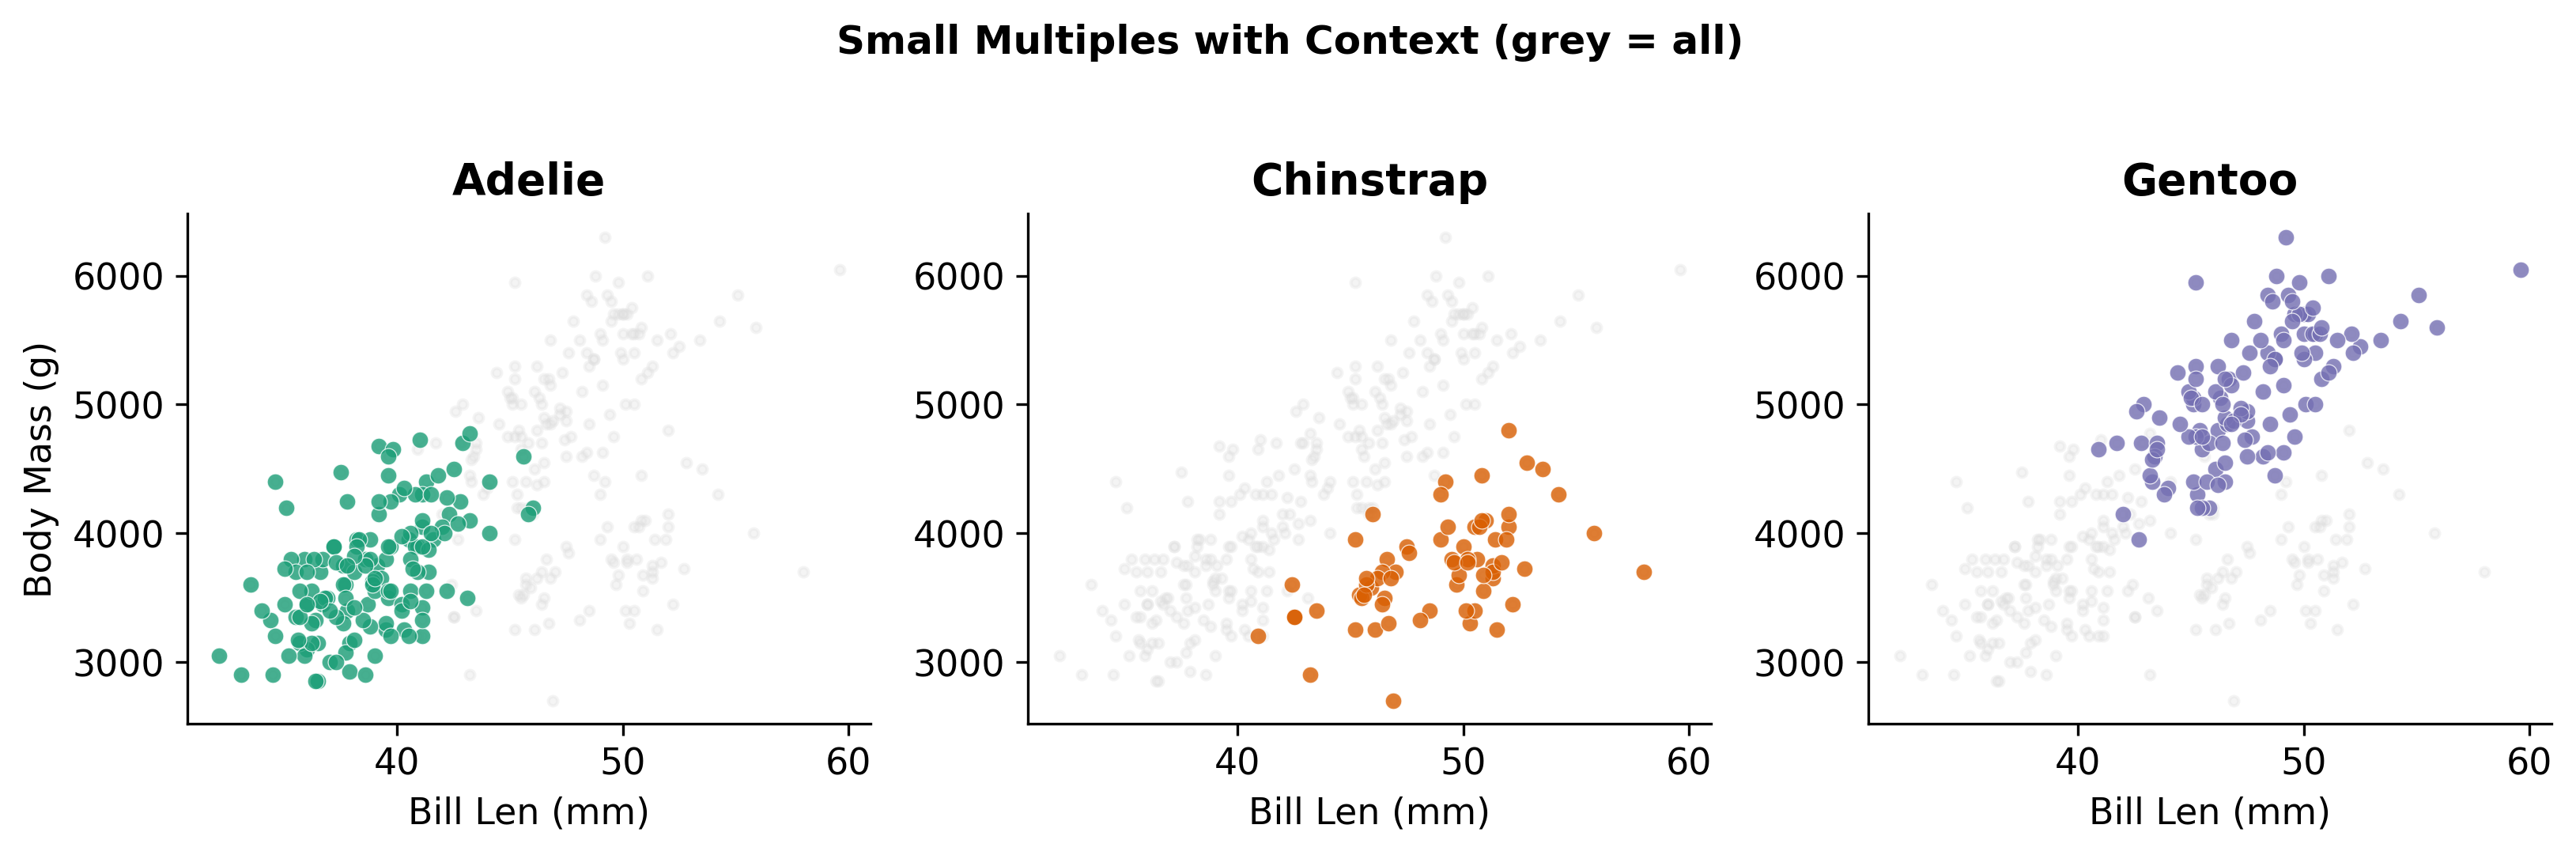
\includegraphics[width=\textwidth]{m1_6_small_multiples_context.png}
\begin{exampleblock}{Data Insight}
    \scriptsize Drop the facet column from the background data. plotnine draws that layer in \emph{every} panel because it has no facet variable to split on.
\end{exampleblock}
\end{column}
\end{columns}
\end{frame}

% ── 168 ──
\begin{frame}{When Faceting Fails: Too Many Panels}
\smark{168/300}
\begin{columns}[T]
\begin{column}{0.50\textwidth}
\begin{itemize}
    \item $>$12 panels $\to$ panels become too small to read
    \item $>$20 panels $\to$ pattern detection collapses
    \item Alternatives when you have many categories: aggregate, sample, or use interactive zoom
    \item Hierarchical faceting (\texttt{ggforce::facet\_zoom}) for detail within context
\end{itemize}
\end{column}
\begin{column}{0.47\textwidth}
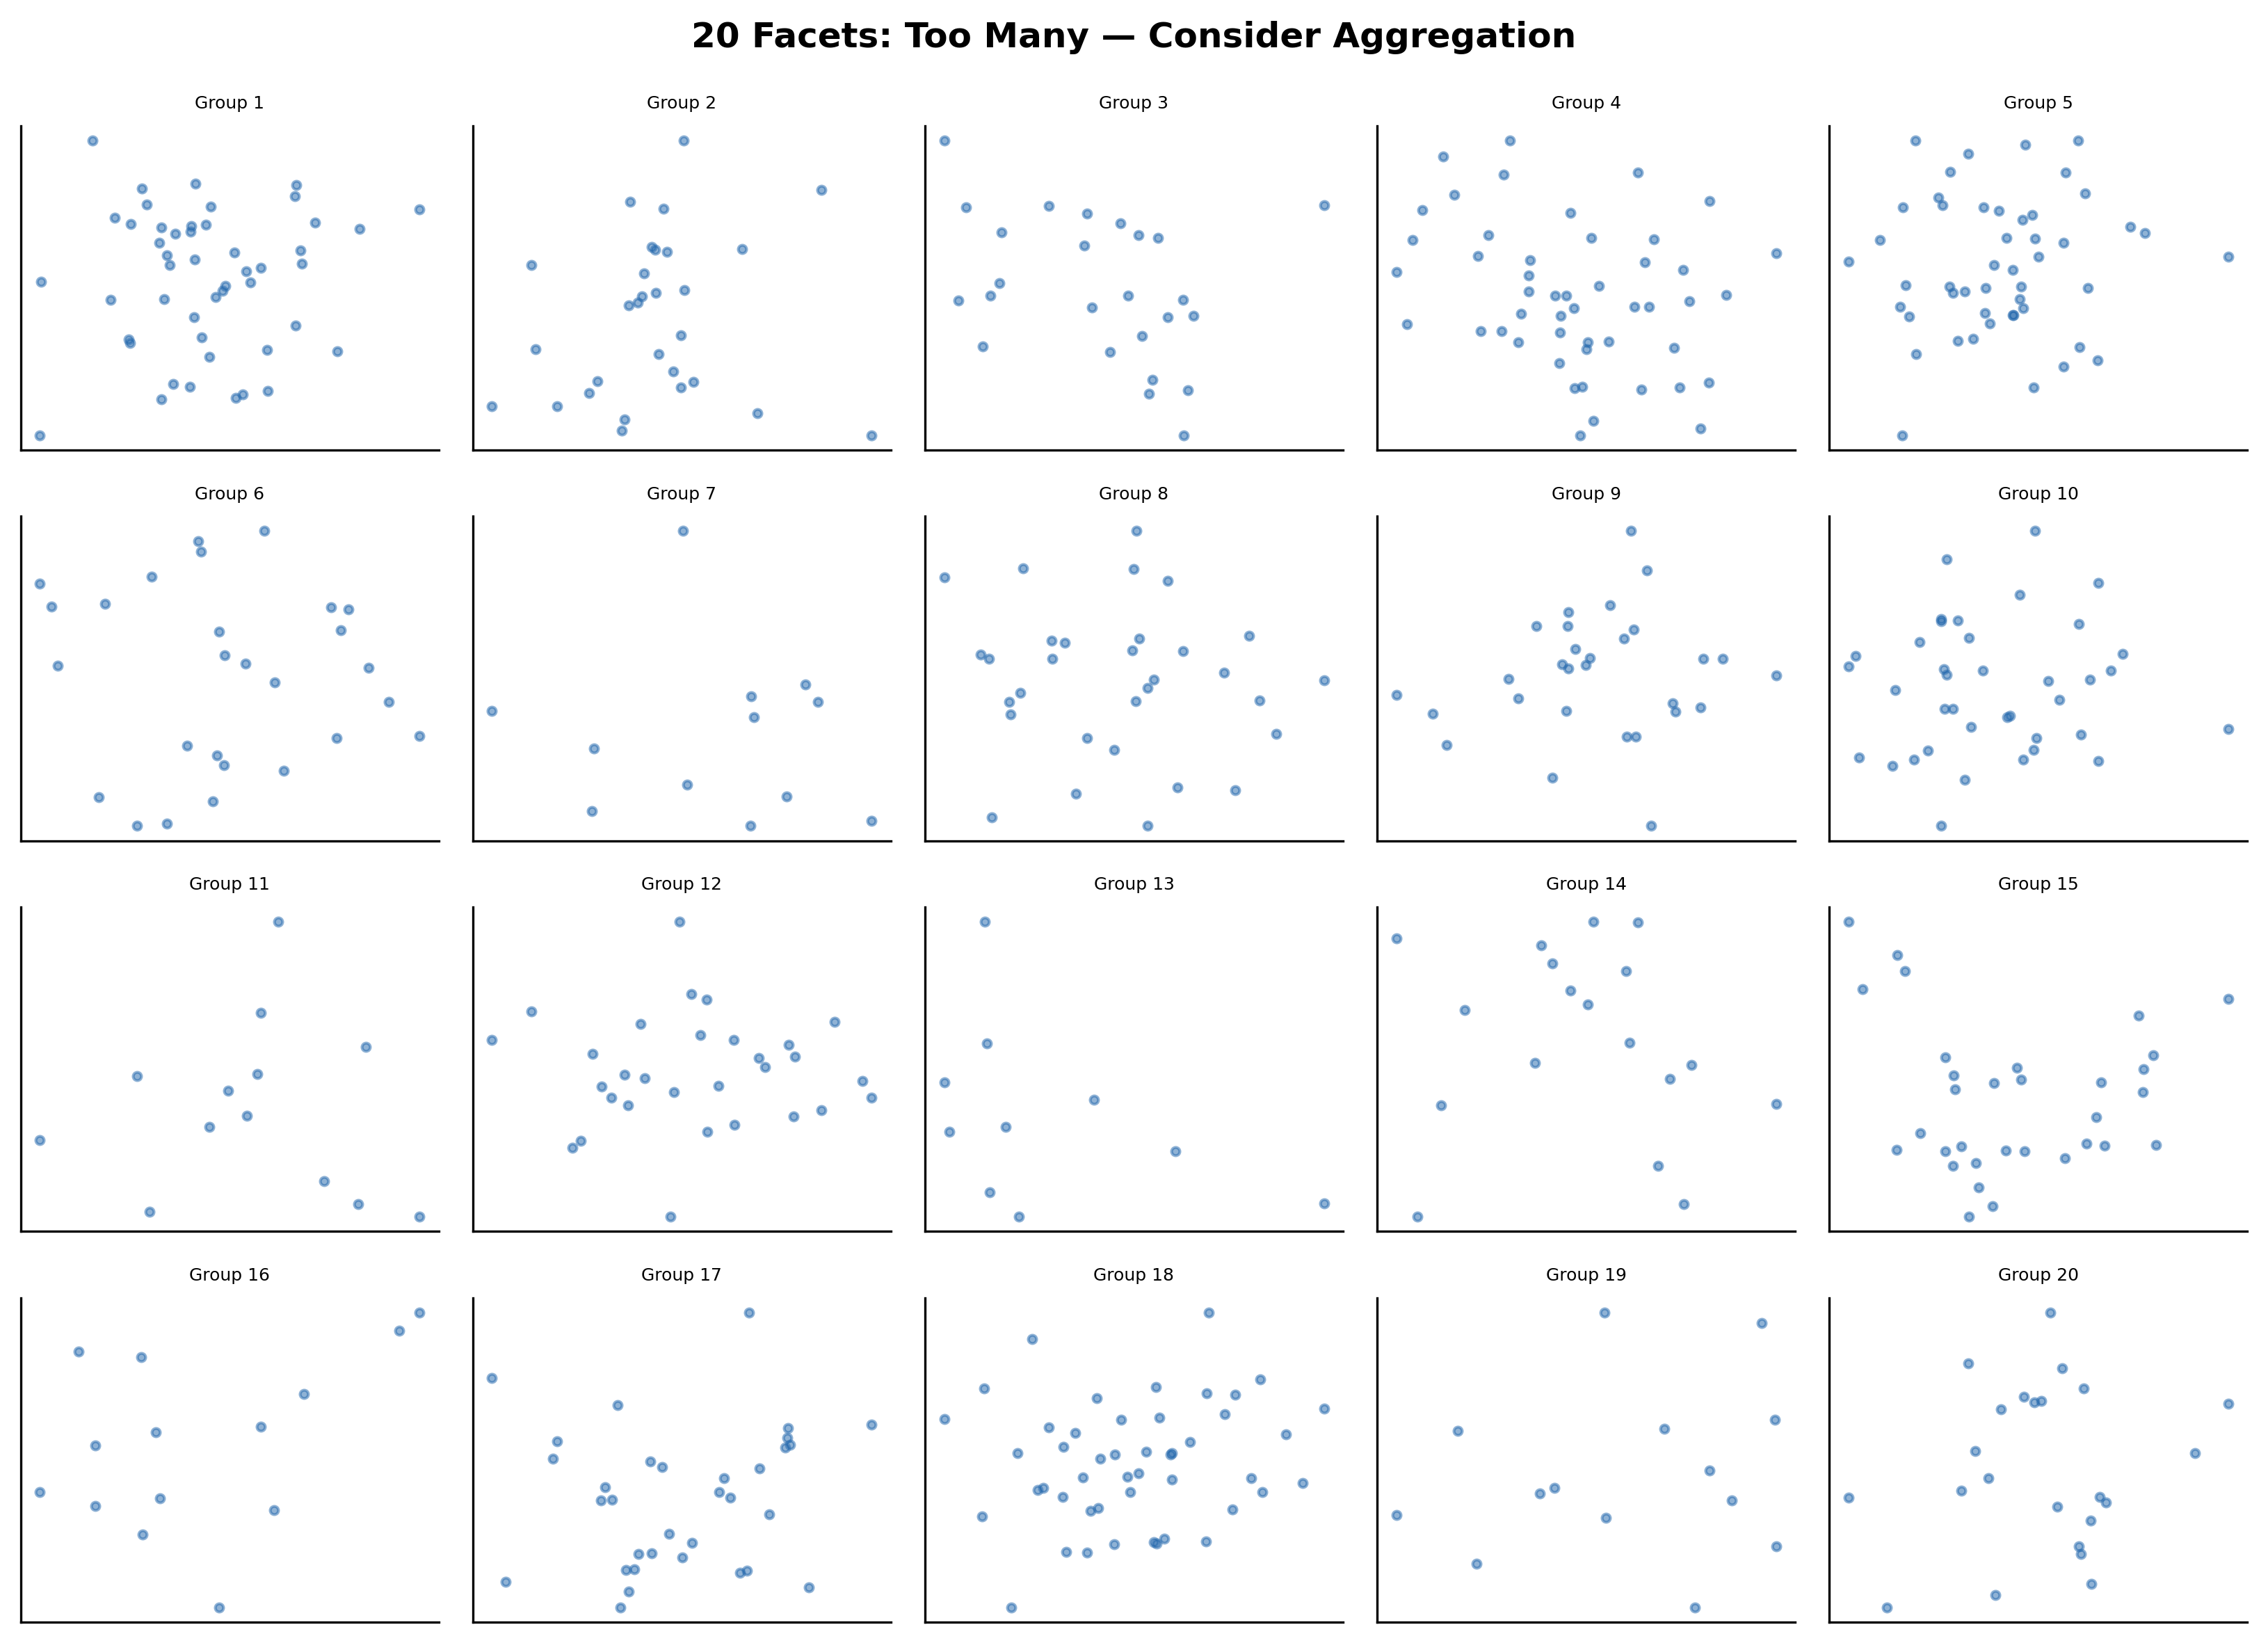
\includegraphics[width=\textwidth]{m1_6_too_many_facets.png}
\begin{alertblock}{Pro-Tip}
    \scriptsize If you have 50 US states, don't facet all 50. Facet by \textbf{region} (5 panels) and use color for states within each region.
\end{alertblock}
\end{column}
\end{columns}
\end{frame}

% ── 169 ──
\begin{frame}{Facet Zoom: Detail Within Context}
\smark{169/300}
\centering
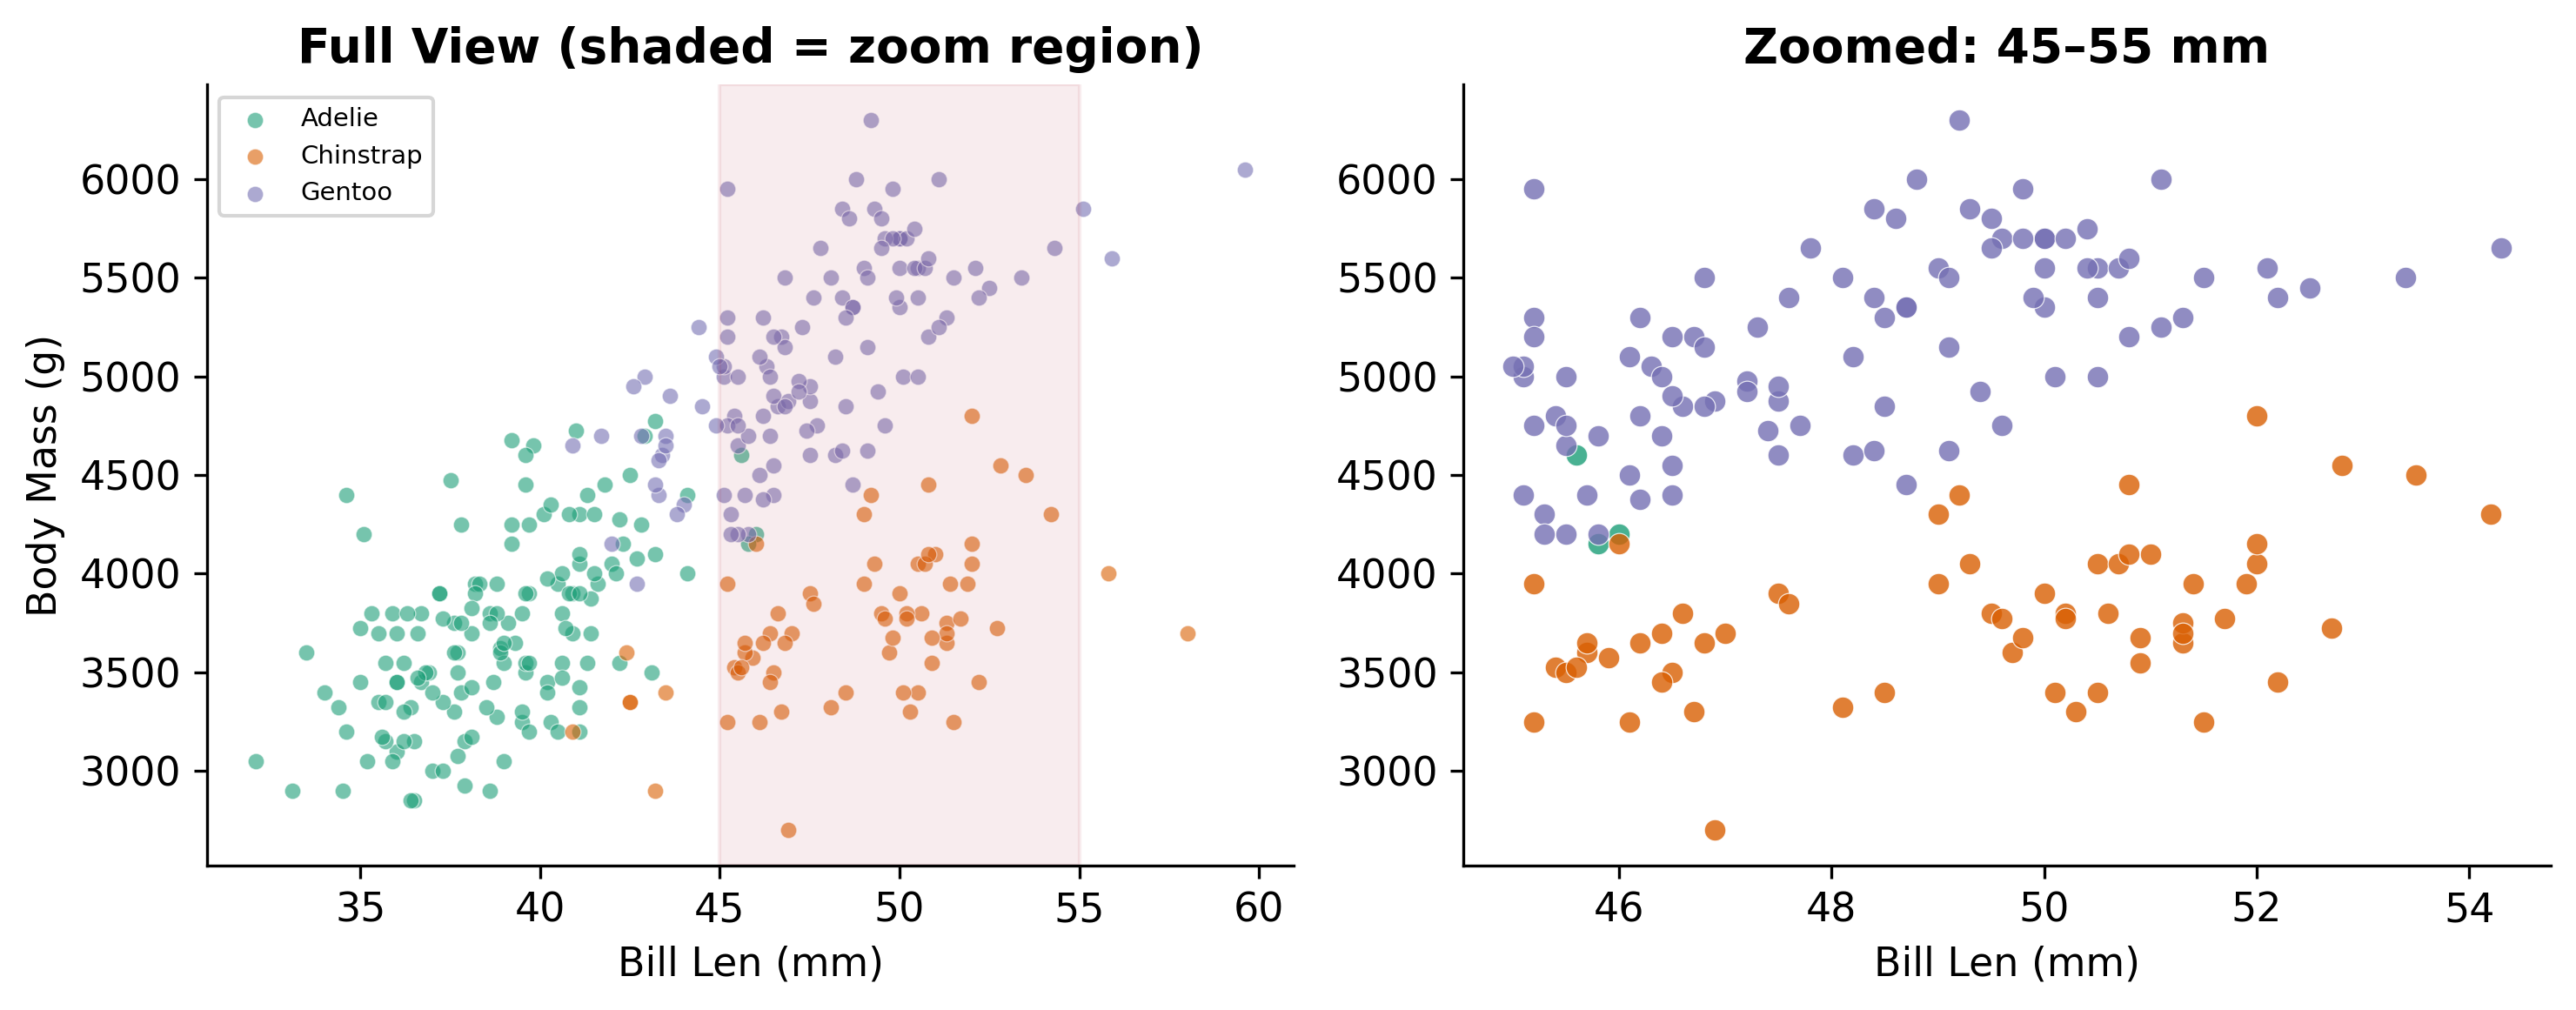
\includegraphics[width=0.85\textwidth]{m1_6_facet_zoom.png}

\vspace{0.2cm}
\begin{columns}[T]
\begin{column}{0.48\textwidth}
\begin{exampleblock}{Data Insight}
    \scriptsize Left panel shows the full data with the zoom region shaded. Right panel shows only 45--55\,mm bill length, enlarged. Both panels share the same $y$-axis for honest comparison.
\end{exampleblock}
\end{column}
\begin{column}{0.48\textwidth}
\begin{alertblock}{Pro-Tip}
    \scriptsize In R, \texttt{ggforce::facet\_zoom(xlim=c(45,55))} does this automatically. In Python, use two subplot axes with shared $y$.
\end{alertblock}
\end{column}
\end{columns}
\end{frame}

% ── 170 ──
\begin{frame}[fragile]{Facet Zoom --- Code}\smark{170/300}
\begin{columns}[T]
\begin{column}{0.48\textwidth}
\begin{lstlisting}[style=Rstyle]
library(ggforce)

ggplot(penguins,
  aes(bill_length_mm,
      body_mass_g,
      color = species)) +
  geom_point(alpha = 0.7) +
  facet_zoom(
    xlim = c(45, 55)) +
  theme_minimal()
\end{lstlisting}
\end{column}
\begin{column}{0.48\textwidth}
\begin{lstlisting}[style=Pystyle]
# Manual in matplotlib
fig, (ax1, ax2) = plt.subplots(
    1, 2, sharey=True)
# ax1: full view
ax1.scatter(x, y)
ax1.axvspan(45, 55, alpha=0.1)
# ax2: zoomed
zoom = df[(df.x>=45)&(df.x<=55)]
ax2.scatter(zoom.x, zoom.y)
ax2.set_xlim(45, 55)
\end{lstlisting}
\end{column}
\end{columns}
\end{frame}

% ── 171 ──
\begin{frame}{Faceting Other Geoms: Histograms}
\smark{171/300}
\centering
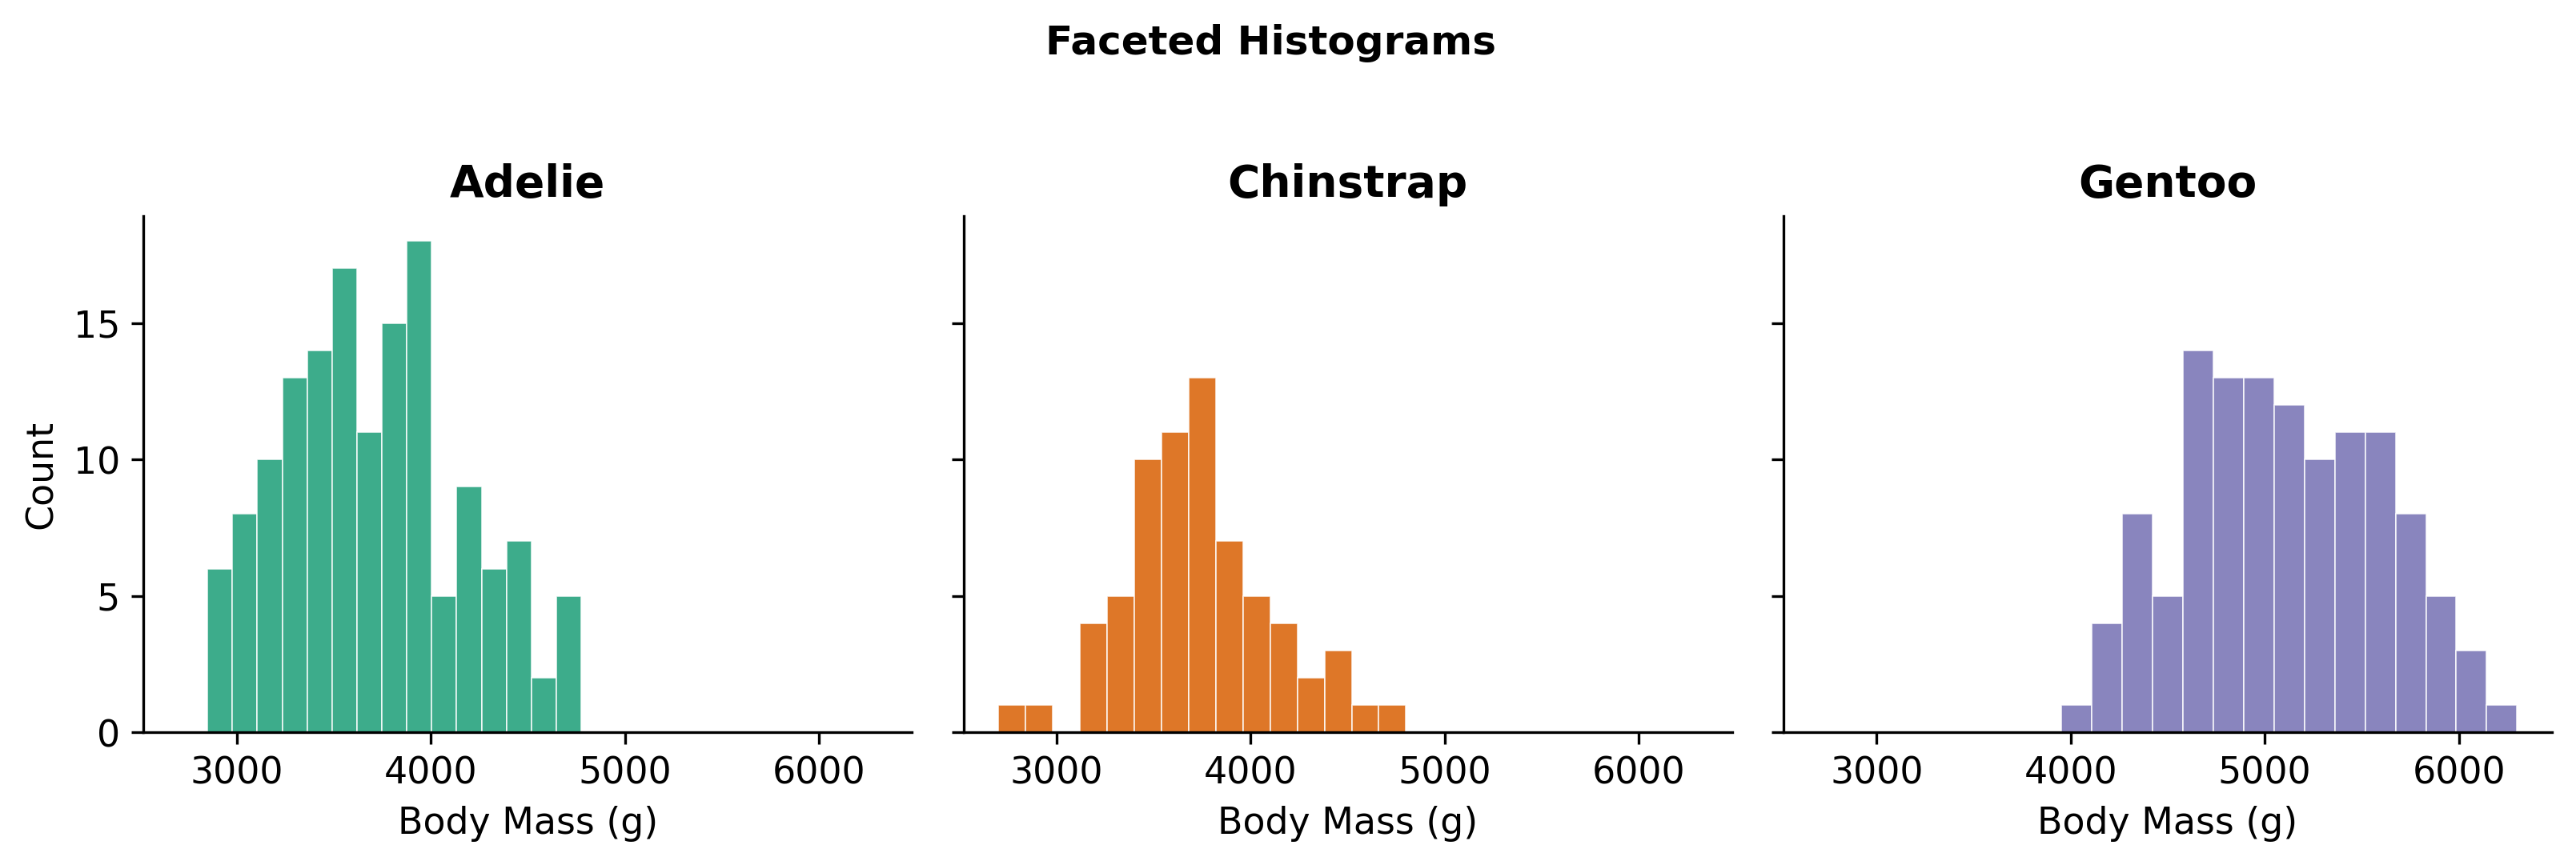
\includegraphics[width=0.85\textwidth]{m1_6_facet_hist.png}

\vspace{0.2cm}
\begin{exampleblock}{Data Insight}
    \scriptsize Faceted histograms solve the grouped-histogram occlusion problem from Module 1.4. Each species' distribution is unobstructed, and the shared $x$-axis makes location comparison valid.
\end{exampleblock}
\end{frame}

% ── 172 ──
\begin{frame}[fragile]{Faceted Histograms --- Code}\smark{172/300}
\begin{columns}[T]
\begin{column}{0.48\textwidth}
\begin{lstlisting}[style=Rstyle]
ggplot(penguins,
  aes(body_mass_g,
      fill = species)) +
  geom_histogram(bins = 15,
    color = "white") +
  facet_wrap(~species) +
  theme(legend.position="none")
\end{lstlisting}
\end{column}
\begin{column}{0.48\textwidth}
\begin{lstlisting}[style=Pystyle]
(ggplot(penguins,
   aes("body_mass_g",
       fill="species"))
 + geom_histogram(bins=15,
     color="white")
 + facet_wrap("~species")
 + theme(legend_position="none"))
\end{lstlisting}
\end{column}
\end{columns}
\vspace{0.2cm}
\begin{alertblock}{Pro-Tip}
    \scriptsize Faceted distributions are almost always preferable to stacked or overlaid histograms when you have 3+ groups.
\end{alertblock}
\end{frame}

% ── 173 ──
\begin{frame}{Faceting Lines and Bars}
\smark{173/300}
\begin{columns}[T]
\begin{column}{0.50\textwidth}
    \textbf{Faceted lines:}
    \begin{itemize}
        \item One panel per time series (e.g., per country)
        \item Avoids ``spaghetti plot'' problem ($>$5 lines)
        \item Shared $x$ (time) axis; free $y$ if scales differ
    \end{itemize}
    \vspace{0.2cm}
    \textbf{Faceted bars:}
    \begin{itemize}
        \item One panel per category of a second variable
        \item Replaces dodged bars when groups $>$3
        \item Cleaner than grouped bar charts
    \end{itemize}
\end{column}
\begin{column}{0.47\textwidth}
\begin{exampleblock}{Data Insight}
    \scriptsize The spaghetti-to-facet refactor is one of the highest-impact improvements you can make: 10 overlapping lines $\to$ 10 clear panels, zero information lost.
\end{exampleblock}
\vspace{0.2cm}
\begin{alertblock}{Pro-Tip}
    \scriptsize For faceted bars, ensure category order is consistent across panels. Use \texttt{fct\_reorder()} \textbf{globally}, not per-panel.
\end{alertblock}
\end{column}
\end{columns}
\end{frame}

% ── 174 ──
\begin{frame}[fragile]{Faceted Lines --- Code}\smark{174/300}
\begin{columns}[T]
\begin{column}{0.48\textwidth}
\begin{lstlisting}[style=Rstyle]
# Spaghetti -> facets
ggplot(economics_long,
  aes(date, value)) +
  geom_line(color = "#2166AC") +
  facet_wrap(~variable,
    scales = "free_y",
    ncol = 1) +
  theme_minimal()
\end{lstlisting}
\end{column}
\begin{column}{0.48\textwidth}
\begin{lstlisting}[style=Pystyle]
(ggplot(econ_long,
   aes("date","value"))
 + geom_line(color="#B2182B")
 + facet_wrap("~variable",
     scales="free_y", ncol=1))

# seaborn
g = sns.FacetGrid(econ_long,
    row="variable",
    sharey=False, height=2)
g.map(plt.plot, "date", "value")
\end{lstlisting}
\end{column}
\end{columns}
\end{frame}

% ── 175 ──
\begin{frame}{\texttt{facet\_wrap} vs.\ \texttt{facet\_grid}: Decision Guide}
\smark{175/300}
\centering\small
\begin{tabular}{@{}lll@{}}
    \toprule
    \textbf{Criterion} & \texttt{facet\_wrap} & \texttt{facet\_grid} \\
    \midrule
    Variables       & 1 (or interaction) & 2 (row + col) \\
    Layout          & Wraps into rows    & Fixed matrix \\
    Empty cells     & Skipped            & Shown (informative) \\
    Free scales     & \texttt{scales="free"} & \texttt{scales="free"} \\
    Best when       & Single splitter    & Two-way comparison \\
    Fails when      & $>$12 panels       & Sparse matrix \\
    \bottomrule
\end{tabular}

\vspace{0.3cm}
\begin{exampleblock}{Data Insight}
    \scriptsize Use \texttt{facet\_wrap} by default. Switch to \texttt{facet\_grid} only when you explicitly need rows and columns to encode two different variables.
\end{exampleblock}
\end{frame}

% ── 176 ──
\begin{frame}{Labeller Functions: Customizing Panel Titles}
\smark{176/300}
\begin{columns}[T]
\begin{column}{0.50\textwidth}
\begin{itemize}
    \item Default: bare factor level (e.g., ``Adelie'')
    \item \texttt{label\_both}: ``species: Adelie''
    \item \texttt{label\_value}: ``Adelie'' (default)
    \item \texttt{label\_wrap\_gen(width=15)}: wraps long labels
    \item Custom: \texttt{labeller = as\_labeller(named\_vector)}
\end{itemize}
\end{column}
\begin{column}{0.47\textwidth}
\begin{alertblock}{Pro-Tip}
    \scriptsize When faceting by a numeric variable (e.g., \texttt{cyl}), \texttt{label\_both} prevents ambiguity: ``cyl: 4'' vs.\ just ``4''.
\end{alertblock}
\vspace{0.2cm}
\begin{exampleblock}{Data Insight}
    \scriptsize In plotnine, \texttt{labeller} works identically. In seaborn, modify titles via \texttt{g.set\_titles("\{col\_name\}")}.
\end{exampleblock}
\end{column}
\end{columns}
\end{frame}

% ── 177 ──
\begin{frame}[fragile]{Labeller --- Code}\smark{177/300}
\begin{columns}[T]
\begin{column}{0.48\textwidth}
\begin{lstlisting}[style=Rstyle]
# label_both: "species: Adelie"
facet_wrap(~species,
  labeller = label_both)

# Custom names
custom <- c(
  Adelie = "Adelie (n=146)",
  Gentoo = "Gentoo (n=119)")
facet_wrap(~species,
  labeller =
    as_labeller(custom))
\end{lstlisting}
\end{column}
\begin{column}{0.48\textwidth}
\begin{lstlisting}[style=Pystyle]
# plotnine: same syntax
facet_wrap("~species",
    labeller="label_both")

# seaborn: manual titles
g = sns.FacetGrid(...)
g.set_titles("{col_name}")
# or iterate:
for ax, title in zip(
    g.axes.flat, custom_list):
    ax.set_title(title)
\end{lstlisting}
\end{column}
\end{columns}
\end{frame}

% ── 178 ──
\begin{frame}{Margin Panels: \texttt{facet\_grid(margins = TRUE)}}\smark{178/300}
\begin{columns}[T]
\begin{column}{0.50\textwidth}
\begin{itemize}
    \item Adds a ``(all)'' panel that shows the \textbf{aggregate} alongside the facets
    \item Only available in \texttt{facet\_grid()}, not \texttt{facet\_wrap()}
    \item Provides context without the grey-background trick
    \item Useful for QC: does the aggregate pattern match the sum of parts?
\end{itemize}
\end{column}
\begin{column}{0.47\textwidth}
\begin{alertblock}{Pro-Tip}
    \scriptsize \texttt{facet\_grid(species \textasciitilde\ island, margins = TRUE)} adds both an ``all species'' row and an ``all islands'' column. Use \texttt{margins = "species"} to add only one.
\end{alertblock}
\vspace{0.2cm}
\begin{exampleblock}{Data Insight}
    \scriptsize plotnine does \textbf{not} support \texttt{margins} as of 2024. Workaround: duplicate the data with an ``All'' category appended and facet on the combined factor.
\end{exampleblock}
\end{column}
\end{columns}
\end{frame}

% ── 179 ──
\begin{frame}{Module 1.6 --- Key Takeaways}\smark{179/300}
\begin{enumerate}
    \item \textbf{Small multiples} replace color when categories exceed 5--6.
    \item \textbf{\texttt{facet\_wrap}} for one splitting variable; \textbf{\texttt{facet\_grid}} for two.
    \item \textbf{Default to fixed scales.} Free scales hide cross-panel comparisons.
    \item \textbf{Grey background context} shows each group relative to the whole.
    \item \textbf{$>$12 panels} means panels are too small. Aggregate or use interactive zoom.
    \item \textbf{Panel order = factor order.} Control it before plotting.
\end{enumerate}
\end{frame}

% ── 180 ──
\begin{frame}{}\smark{180/300}
\centering\vspace{1.5cm}
{\Large\textbf{Module 1.6 Complete}}\\[0.5cm]
You can now decompose any complex plot into readable small-multiple panels with \texttt{facet\_wrap} and \texttt{facet\_grid}, with controlled scales, layout, labels, and contextual backgrounds.\\[0.5cm]
\textbf{Next:} Module 1.7 --- Coordinate Systems and Transformations.
\end{frame}

% ═══════════════════════════════════════════════════════
%  MODULE 1.7 — Coordinate Systems and Transformations
% ═══════════════════════════════════════════════════════
\section{Module 1.7 --- Coordinate Systems and Transformations}

% ── 181 ──
\begin{frame}{Module 1.7 --- Roadmap}\smark{181/300}
\begin{enumerate}
    \item Cartesian coordinates: the invisible default
    \item \texttt{coord\_flip()}: when and why to swap axes
    \item \texttt{coord\_polar()}: bar $\to$ Coxcomb $\to$ pie
    \item Log scales: \texttt{scale\_x\_log10} vs.\ \texttt{coord\_trans}
    \item When to log-transform axes vs.\ data
    \item Aspect ratio and banking to 45\textdegree
    \item Reversed and discrete axes
    \item The zoom trap revisited: viewport vs.\ data filter
\end{enumerate}
\end{frame}

% ── 182 ──
\begin{frame}{Cartesian Coordinates: The Invisible Default}
\smark{182/300}
\begin{columns}[T]
\begin{column}{0.50\textwidth}
\begin{itemize}
    \item Every ggplot uses \texttt{coord\_cartesian()} unless overridden
    \item Orthogonal $x$--$y$ axes, equal spacing per unit
    \item \textbf{Zooming}: clips the viewport without dropping data
    \item Contrast with \texttt{scale\_*\_continuous(limits=...)} which \textbf{removes} data outside the range
\end{itemize}
\end{column}
\begin{column}{0.47\textwidth}
\begin{exampleblock}{Data Insight}
    \scriptsize Coordinates act \textbf{after} statistical transformations. A smoother fit on all data, then clipped to a viewport, is different from a smoother fit on filtered data.
\end{exampleblock}
\vspace{0.2cm}
\begin{alertblock}{Pro-Tip}
    \scriptsize When in doubt, always zoom with \texttt{coord\_cartesian()} rather than scale limits.
\end{alertblock}
\end{column}
\end{columns}
\end{frame}

% ── 183 ──
\begin{frame}{The Zoom Trap: Viewport vs.\ Data Filter}
\smark{183/300}
\centering
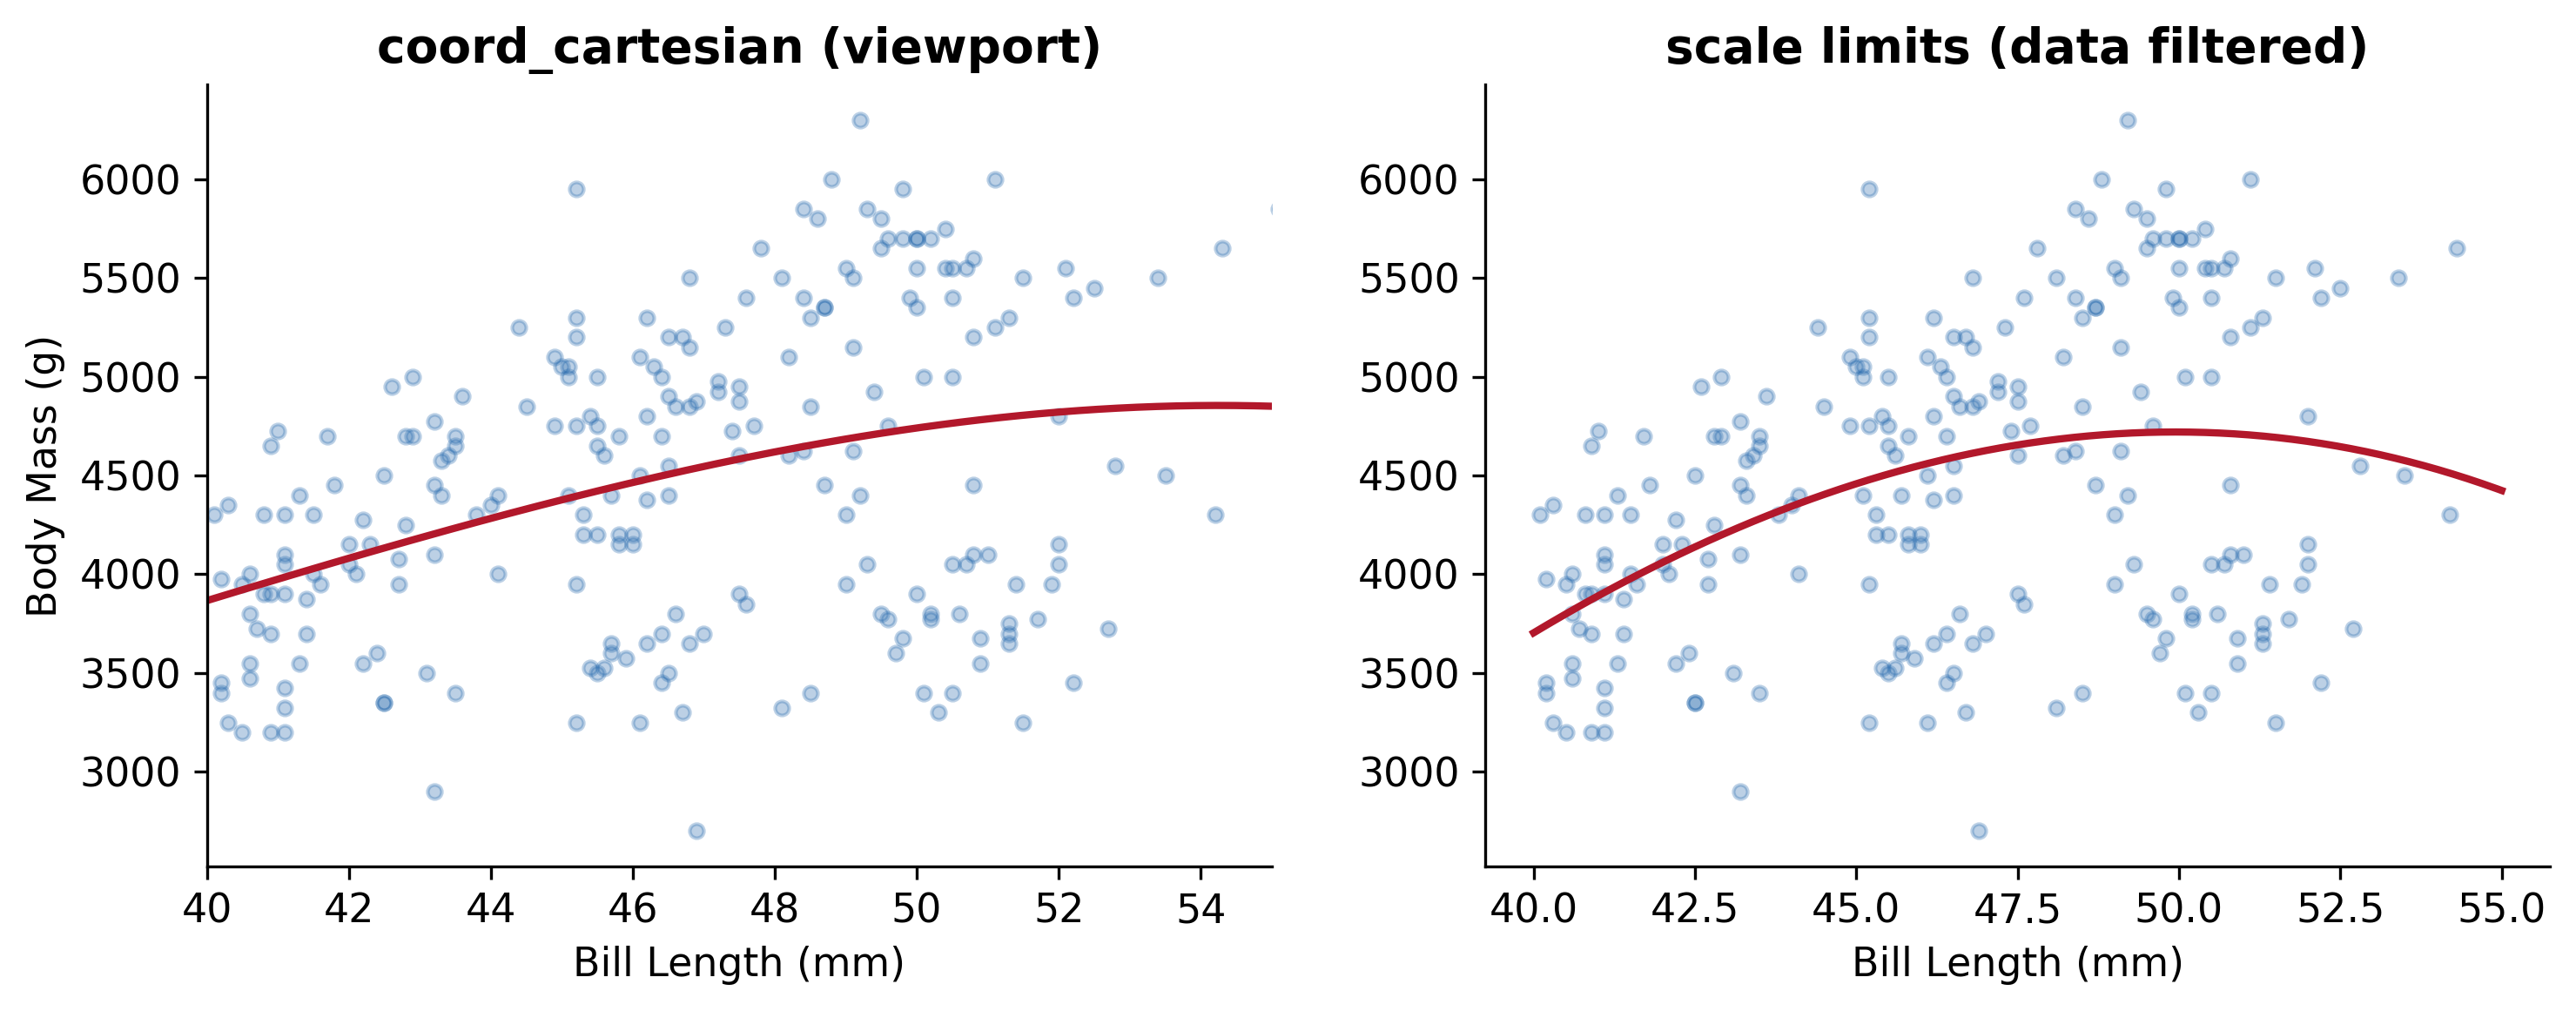
\includegraphics[width=0.88\textwidth]{m1_7_zoom_trap.png}

\vspace{0.2cm}
\begin{columns}[T]
\begin{column}{0.48\textwidth}
\begin{exampleblock}{Data Insight}
    \scriptsize Left: smoother computed on \textbf{all} data, then viewport clipped. Right: data outside 40--55\,mm \textbf{deleted first}, smoother refit on subset. The curve shape differs.
\end{exampleblock}
\end{column}
\begin{column}{0.48\textwidth}
\begin{alertblock}{Pro-Tip}
    \scriptsize This matters whenever a \texttt{stat} layer is present: smooth, boxplot, density, regression. For \texttt{geom\_point()} alone, both methods look identical.
\end{alertblock}
\end{column}
\end{columns}
\end{frame}

% ── 184 ──
\begin{frame}[fragile]{Zoom Trap --- Code}\smark{184/300}
\begin{columns}[T]
\begin{column}{0.48\textwidth}
\begin{lstlisting}[style=Rstyle]
# SAFE: viewport zoom
ggplot(penguins,
  aes(bill_length_mm,
      body_mass_g)) +
  geom_point() +
  geom_smooth() +
  coord_cartesian(
    xlim = c(40, 55))
\end{lstlisting}
\scriptsize Smoother on \textbf{all} data.
\end{column}
\begin{column}{0.48\textwidth}
\begin{lstlisting}[style=Rstyle]
# DANGEROUS: data filter
ggplot(penguins,
  aes(bill_length_mm,
      body_mass_g)) +
  geom_point() +
  geom_smooth() +
  scale_x_continuous(
    limits = c(40, 55))
\end{lstlisting}
\scriptsize Points outside \textbf{removed}. Smoother refit.
\end{column}
\end{columns}
\end{frame}

% ── 185 ──
\begin{frame}[fragile]{Zoom Trap --- \Python}\smark{185/300}
\begin{columns}[T]
\begin{column}{0.48\textwidth}
\begin{lstlisting}[style=Pystyle]
# plotnine: safe
(ggplot(penguins, aes(
    "bill_length_mm",
    "body_mass_g"))
 + geom_point()
 + geom_smooth()
 + coord_cartesian(
     xlim=(40, 55)))
\end{lstlisting}
\end{column}
\begin{column}{0.48\textwidth}
\begin{lstlisting}[style=Pystyle]
# matplotlib: viewport = safe
ax.set_xlim(40, 55)
# This is a viewport clip,
# equivalent to coord_cartesian.
# matplotlib never drops data
# when you set axis limits.
\end{lstlisting}
\vspace{0.2cm}
\begin{exampleblock}{Data Insight}
    \scriptsize matplotlib's \texttt{set\_xlim} is inherently a viewport operation. The danger is only in the grammar layer (\texttt{scale\_x}).
\end{exampleblock}
\end{column}
\end{columns}
\end{frame}

% ── 186 ──
\begin{frame}{\texttt{coord\_flip}: Swapping Axes}
\smark{186/300}
\centering
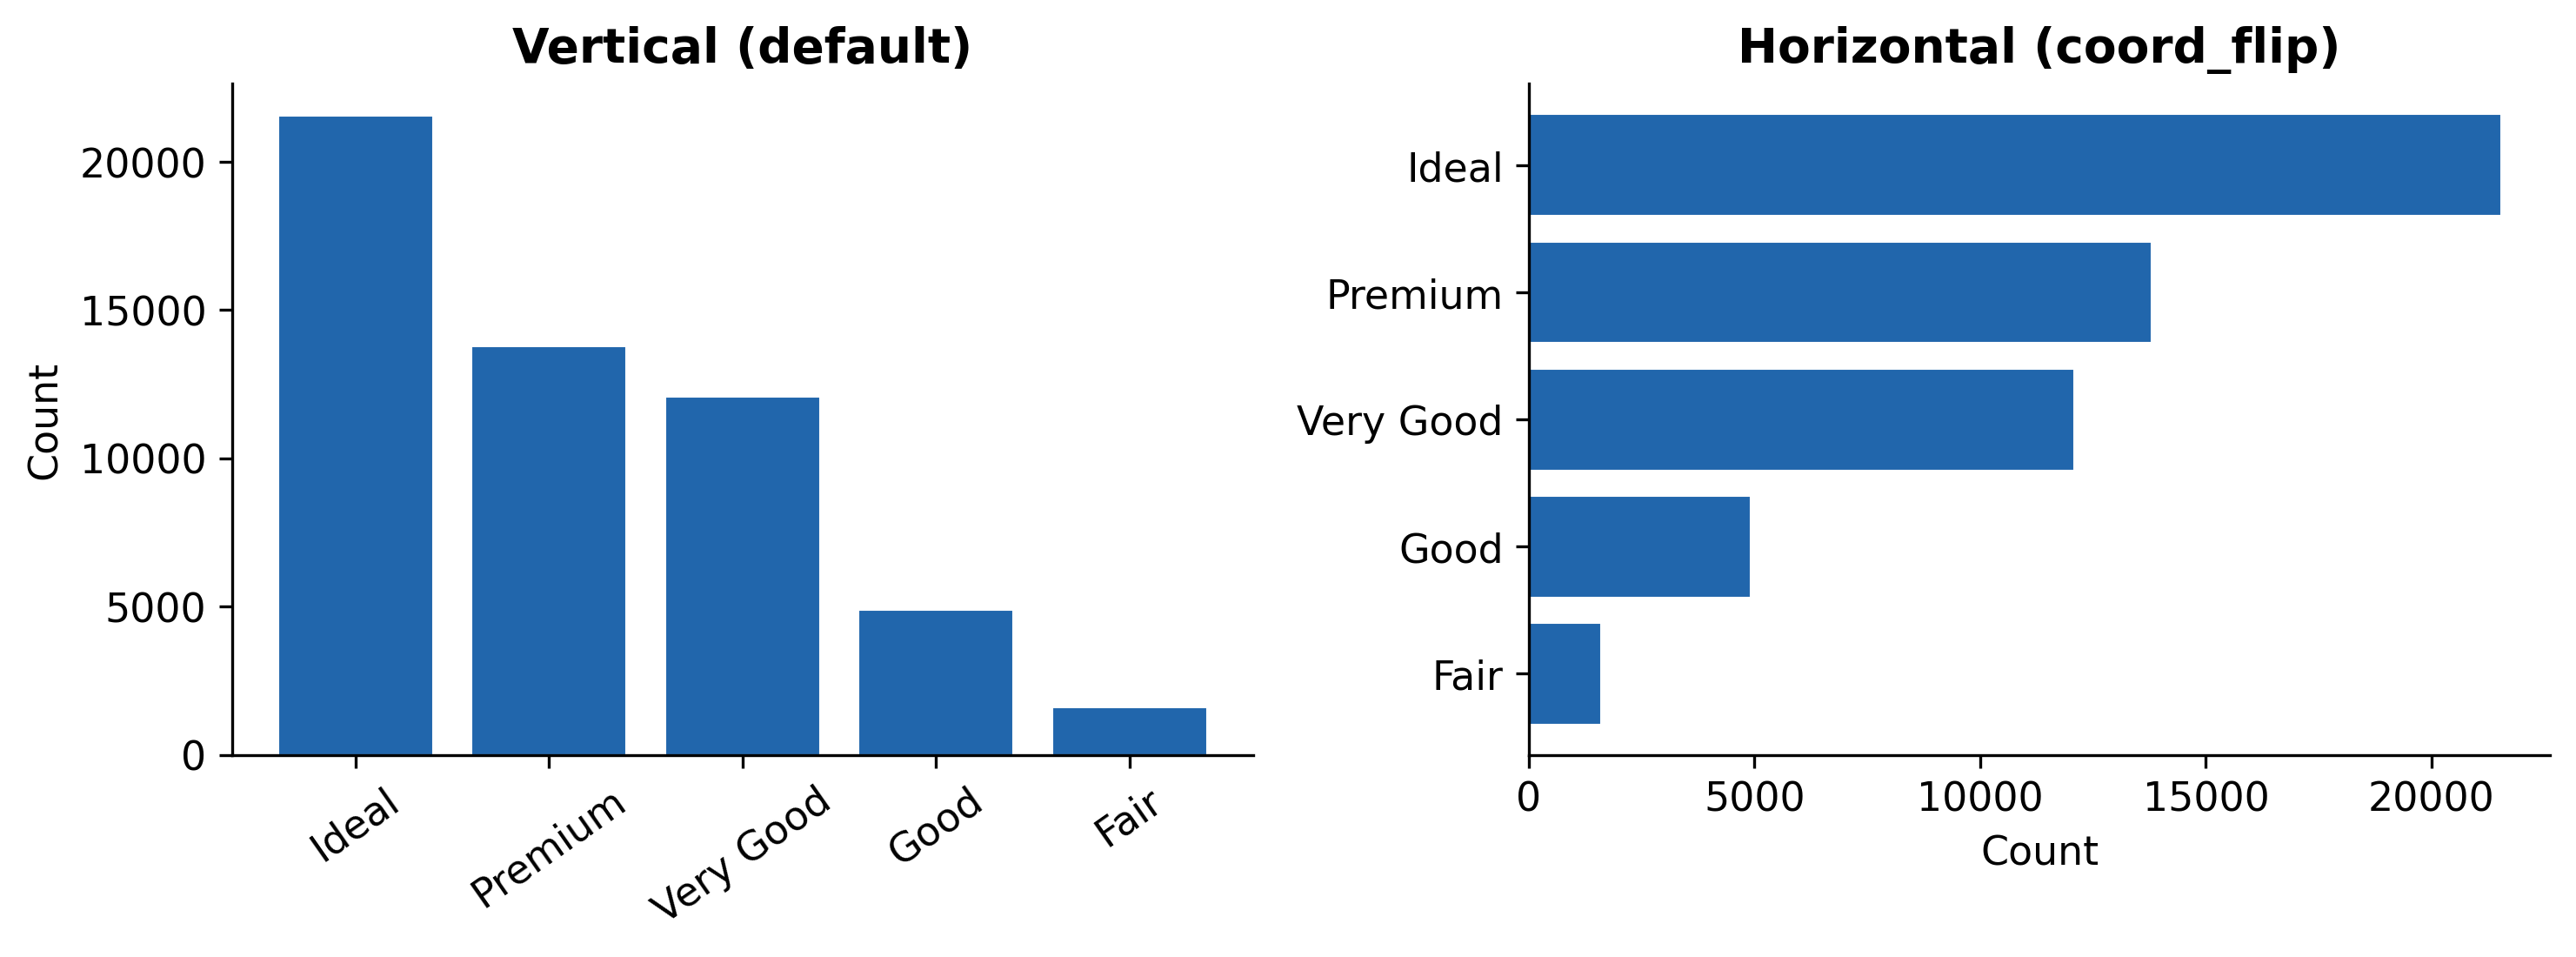
\includegraphics[width=0.88\textwidth]{m1_7_coord_flip.png}

\vspace{0.2cm}
\begin{columns}[T]
\begin{column}{0.48\textwidth}
\begin{itemize}
    \item Transposes $x$ and $y$ axes
    \item Long category labels readable horizontally
    \item Cleveland dot plots and lollipop charts
\end{itemize}
\end{column}
\begin{column}{0.48\textwidth}
\begin{alertblock}{Pro-Tip}
    \scriptsize In ggplot2 v3.3+, many geoms accept horizontal orientation natively. But \texttt{coord\_flip()} is still the universal approach that works with \emph{any} geom.
\end{alertblock}
\end{column}
\end{columns}
\end{frame}

% ── 187 ──
\begin{frame}[fragile]{\texttt{coord\_flip} --- Code}\smark{187/300}
\begin{columns}[T]
\begin{column}{0.48\textwidth}
\begin{lstlisting}[style=Rstyle]
ggplot(diamonds |> count(cut),
  aes(fct_reorder(cut, n),
      n)) +
  geom_col(fill = "#2166AC") +
  coord_flip() +
  labs(x = NULL, y = "Count") +
  theme_minimal()
\end{lstlisting}
\end{column}
\begin{column}{0.48\textwidth}
\begin{lstlisting}[style=Pystyle]
# plotnine
(ggplot(df, aes("cut","n"))
 + geom_col(fill="#B2182B")
 + coord_flip())

# matplotlib: barh directly
plt.barh(df["cut"], df["n"],
         color="#B2182B")
\end{lstlisting}
\vspace{0.1cm}
\begin{exampleblock}{Data Insight}
    \scriptsize matplotlib uses \texttt{barh()} directly. No coord flip needed --- the API offers both orientations as separate functions.
\end{exampleblock}
\end{column}
\end{columns}
\end{frame}

% ── 188 ──
\begin{frame}{\texttt{coord\_polar}: Bar $\to$ Coxcomb $\to$ Pie}
\smark{188/300}
\centering
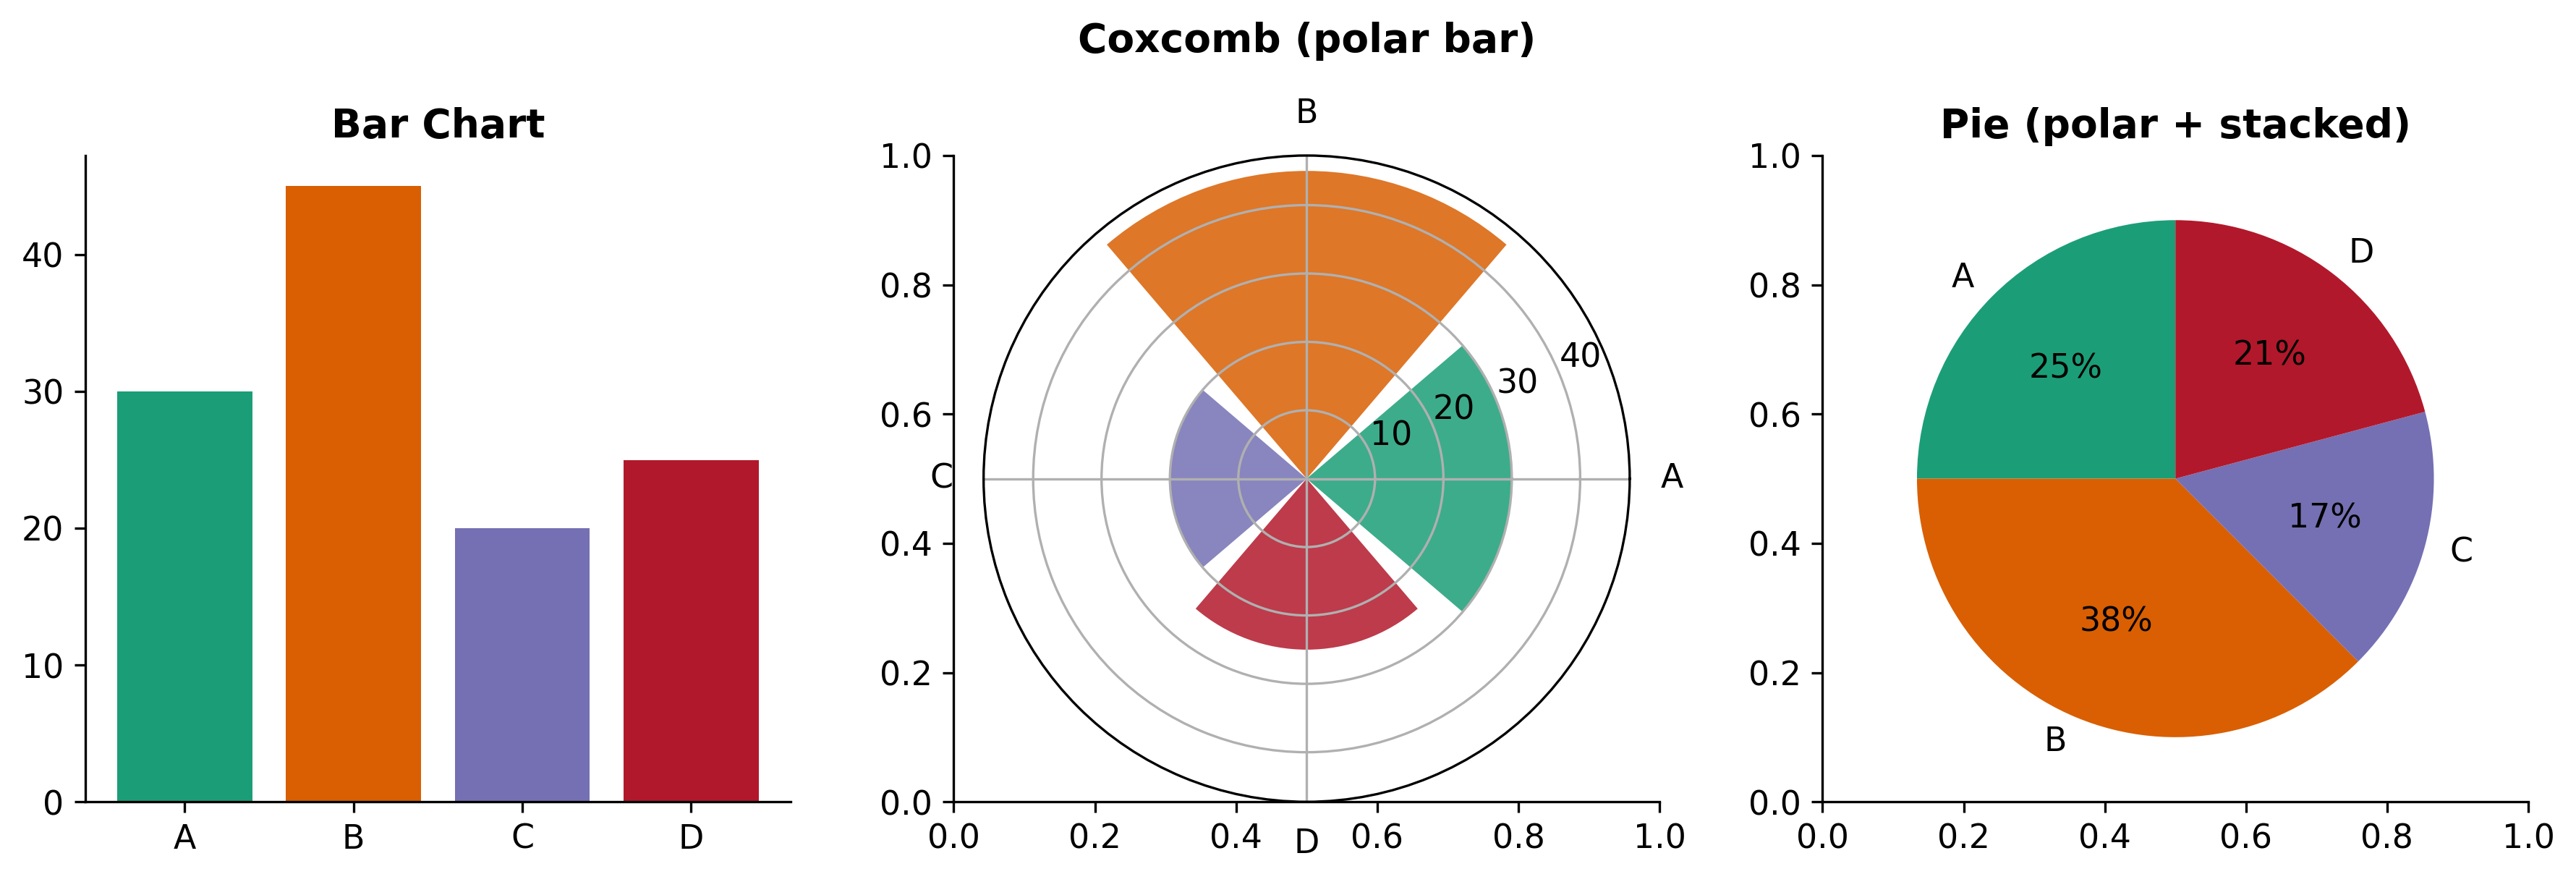
\includegraphics[width=0.92\textwidth]{m1_7_coord_polar.png}

\vspace{0.2cm}
\begin{exampleblock}{Data Insight}
    \scriptsize The grammar makes this explicit: a pie chart is a \textbf{stacked bar in polar coordinates}. \texttt{coord\_polar("y")} wraps the $y$-axis around a circle. A Coxcomb keeps bars at equal angle, varying radius.
\end{exampleblock}
\end{frame}

% ── 189 ──
\begin{frame}[fragile]{\texttt{coord\_polar} --- Code}\smark{189/300}
\begin{columns}[T]
\begin{column}{0.48\textwidth}
\begin{lstlisting}[style=Rstyle]
# Coxcomb (bar in polar)
ggplot(df, aes(x=cat, y=val,
               fill=cat)) +
  geom_col() +
  coord_polar() +
  theme_void()

# Pie (stacked bar in polar)
ggplot(df, aes(x="", y=val,
               fill=cat)) +
  geom_col(width=1) +
  coord_polar("y") +
  theme_void()
\end{lstlisting}
\end{column}
\begin{column}{0.48\textwidth}
\begin{lstlisting}[style=Pystyle]
# plotnine
(ggplot(df, aes("","val",
                fill="cat"))
 + geom_col(width=1)
 + coord_polar("y")
 + theme_void())

# matplotlib
ax.pie(vals, labels=cats,
       autopct="%1.0f%%")
\end{lstlisting}
\vspace{0.1cm}
\begin{alertblock}{Pro-Tip}
    \scriptsize Pie charts: use only for binary or 2--3 slice comparisons. For anything else, bars are more accurate (Cleveland \& McGill, 1984).
\end{alertblock}
\end{column}
\end{columns}
\end{frame}

% ── 190 ──
\begin{frame}{Wind Roses and Radar: Other Polar Uses}
\smark{190/300}
\begin{columns}[T]
\begin{column}{0.50\textwidth}
\begin{itemize}
    \item \textbf{Wind rose}: directional frequency in polar coords (meteorology)
    \item \textbf{Radar/spider chart}: multivariate profile on polar axes
    \item Both use \texttt{coord\_polar()} but with different data mappings
    \item Radar charts are controversial: area distortion, no common baseline
\end{itemize}
\end{column}
\begin{column}{0.47\textwidth}
\begin{alertblock}{Pro-Tip}
    \scriptsize Radar charts \textbf{look impressive} but encode data as area (rank 5) and angle (rank 4). A parallel coordinate plot or bar chart is almost always more accurate. Use radar only for stakeholder dashboards where familiarity outweighs precision.
\end{alertblock}
\end{column}
\end{columns}
\end{frame}

% ── 191 ──
\begin{frame}{Log Scales: When and Why}
\smark{191/300}
\centering
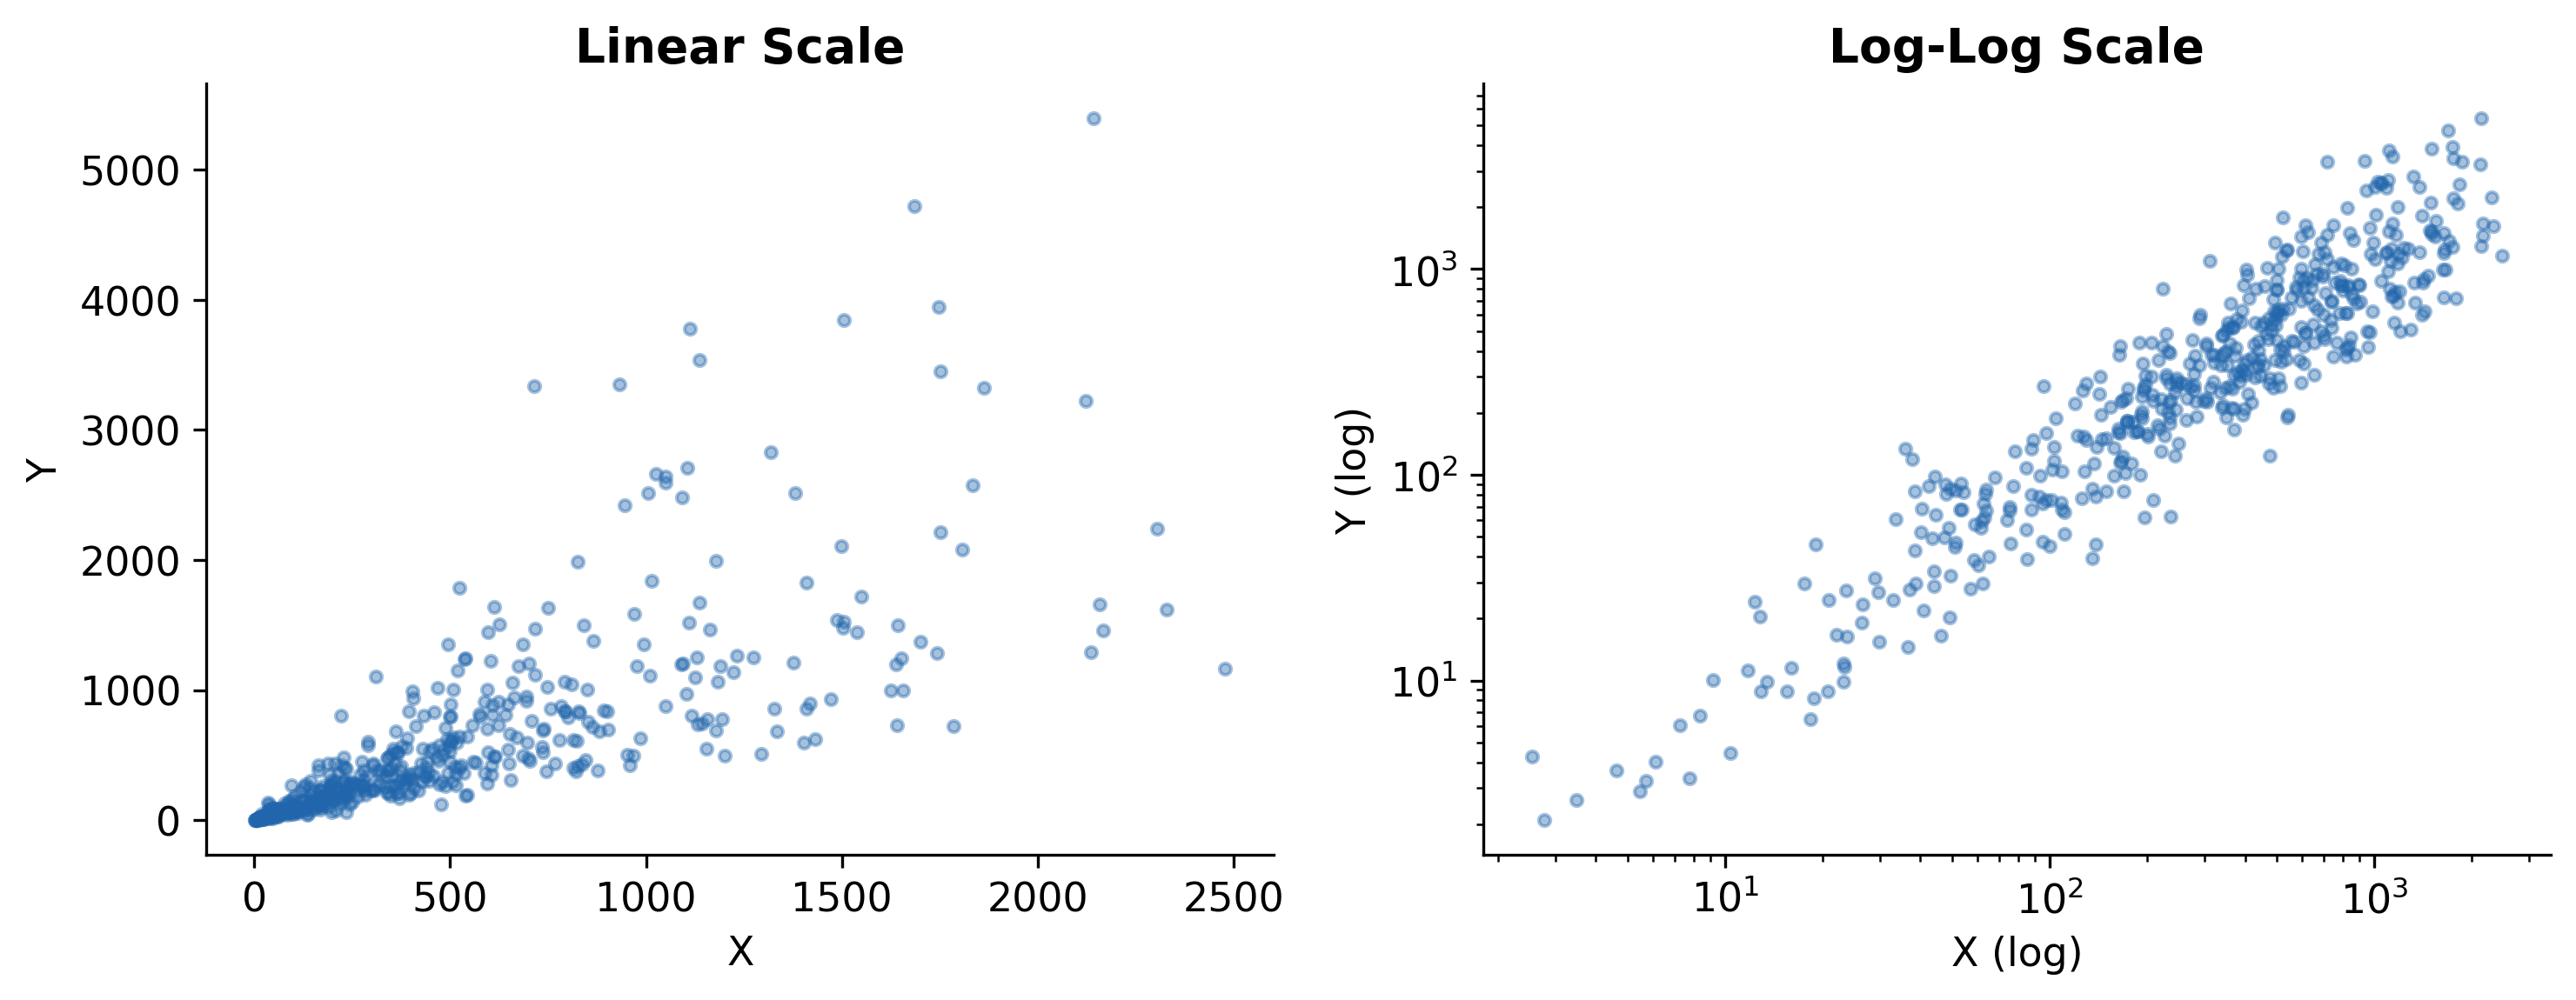
\includegraphics[width=0.88\textwidth]{m1_7_log_scale.png}

\vspace{0.2cm}
\begin{columns}[T]
\begin{column}{0.48\textwidth}
\begin{itemize}
    \item Data spans \textbf{multiple orders of magnitude} (e.g., income, population, gene expression)
    \item Linear scale compresses the lower range into a blob
    \item Log scale spreads the range evenly
\end{itemize}
\end{column}
\begin{column}{0.48\textwidth}
\begin{exampleblock}{Data Insight}
    \scriptsize On the log-log plot, the power-law relationship becomes a straight line. Equal spacing on log axes = equal \emph{ratios}, not equal \emph{differences}.
\end{exampleblock}
\end{column}
\end{columns}
\end{frame}

% ── 192 ──
\begin{frame}[fragile]{Log Scales --- \Rlang}\smark{192/300}
\begin{columns}[T]
\begin{column}{0.55\textwidth}
\begin{lstlisting}[style=Rstyle]
# Log scale on x-axis
ggplot(df, aes(x, y)) +
  geom_point(alpha = 0.4) +
  scale_x_log10() +
  scale_y_log10() +
  annotation_logticks() +
  theme_minimal()

# coord_trans: log transform
# for coord system only
ggplot(df, aes(x, y)) +
  geom_point() +
  coord_trans(x = "log10",
              y = "log10")
\end{lstlisting}
\end{column}
\begin{column}{0.42\textwidth}
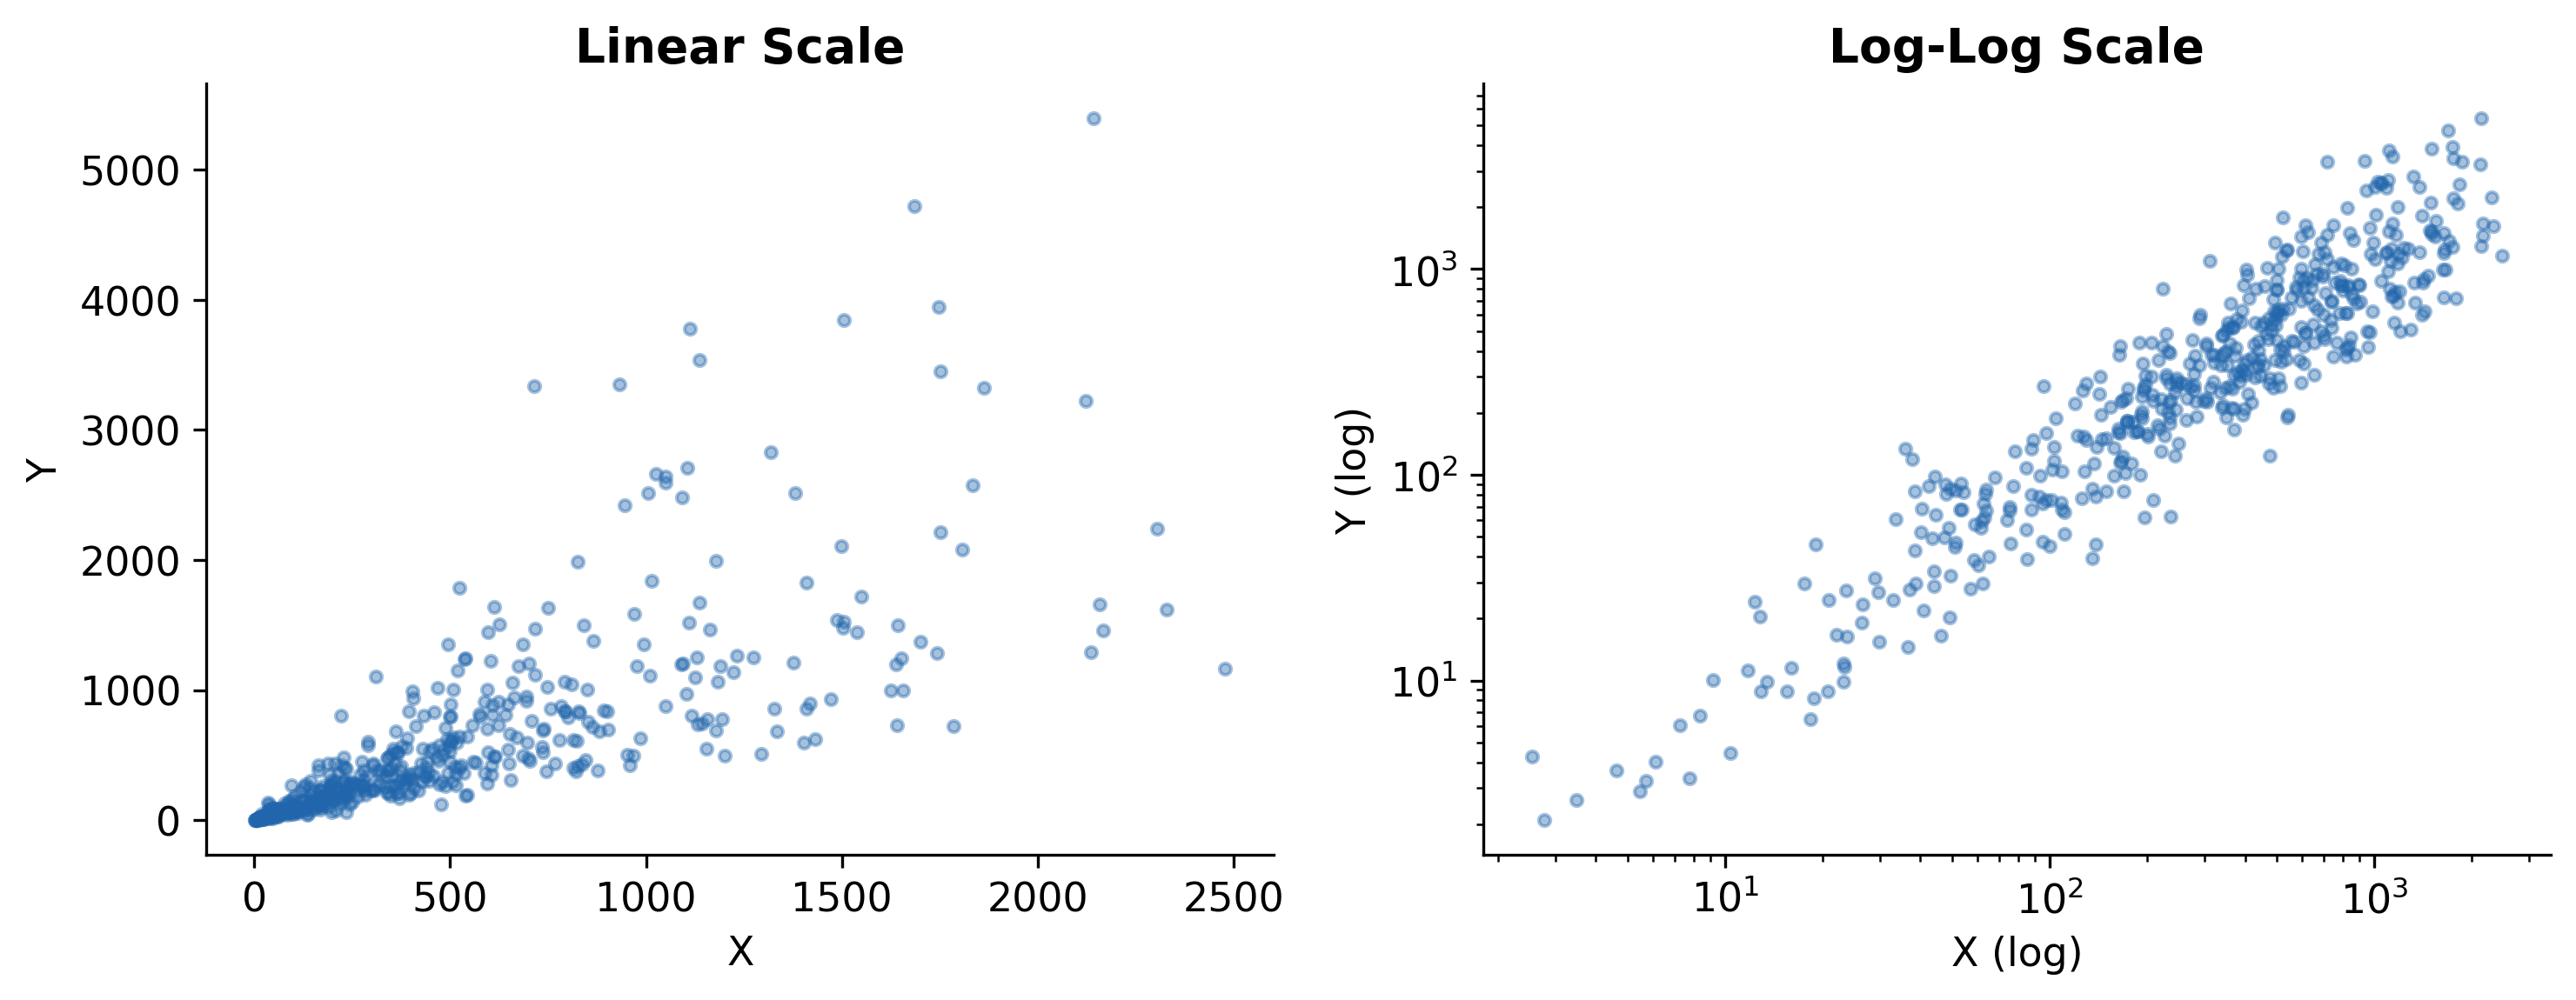
\includegraphics[width=\textwidth]{m1_7_log_scale.png}
\begin{alertblock}{Pro-Tip}
    \scriptsize \texttt{scale\_x\_log10()} transforms \textbf{before} stat layers. \texttt{coord\_trans(x="log10")} transforms \textbf{after}. Smoothers differ between the two.
\end{alertblock}
\end{column}
\end{columns}
\end{frame}

% ── 193 ──
\begin{frame}[fragile]{Log Scales --- \Python}\smark{193/300}
\begin{columns}[T]
\begin{column}{0.55\textwidth}
\begin{lstlisting}[style=Pystyle]
# plotnine
(ggplot(df, aes("x","y"))
 + geom_point(alpha=0.4)
 + scale_x_log10()
 + scale_y_log10())

# matplotlib
ax.set_xscale("log")
ax.set_yscale("log")
# OR
ax.loglog(x, y, "o", alpha=0.4)

# seaborn
sns.scatterplot(data=df, x="x",
    y="y", alpha=0.4)
plt.xscale("log"); plt.yscale("log")
\end{lstlisting}
\end{column}
\begin{column}{0.42\textwidth}
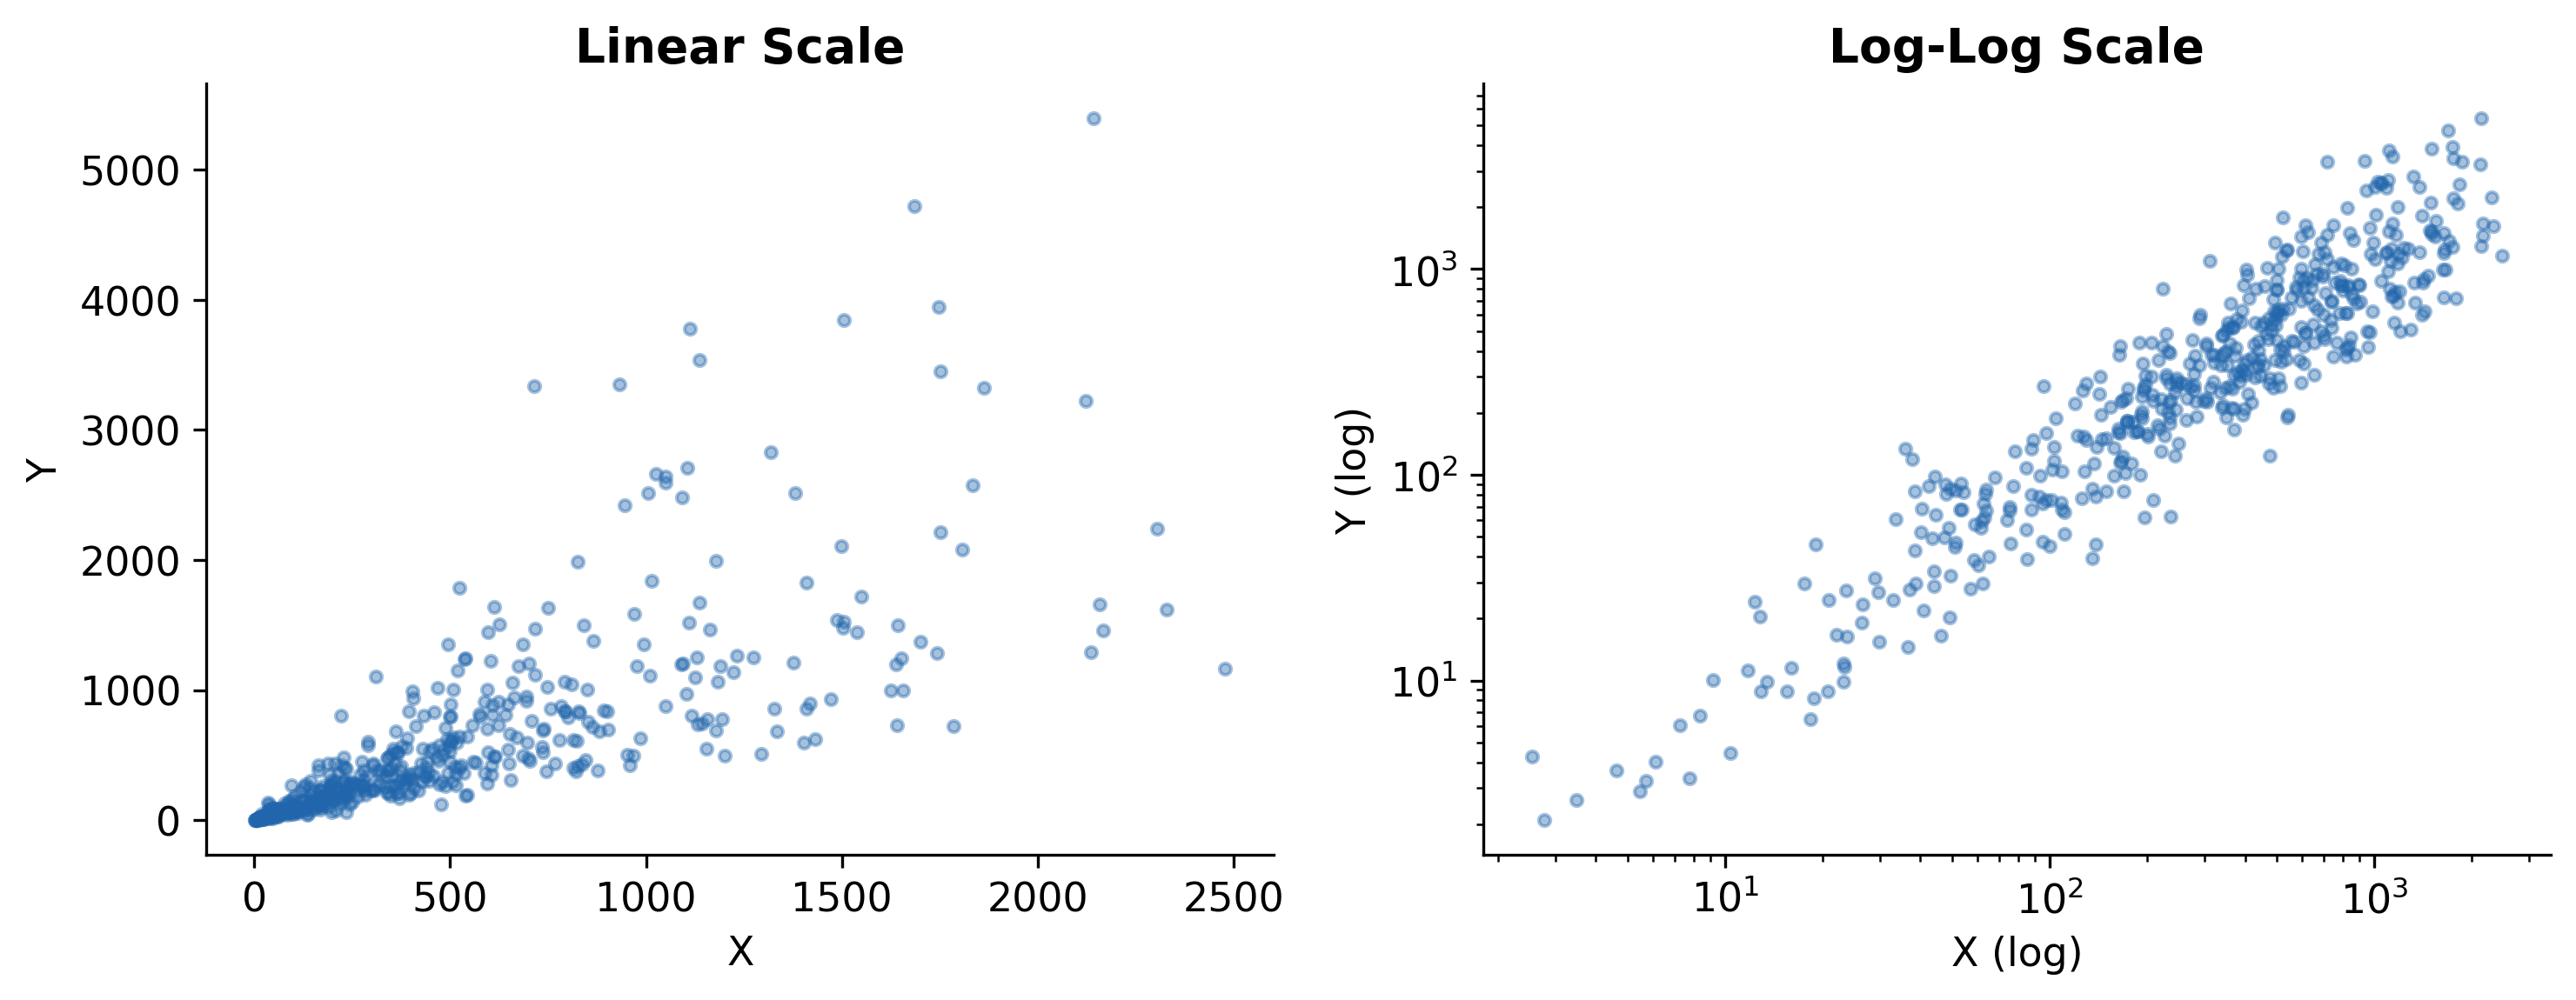
\includegraphics[width=\textwidth]{m1_7_log_scale.png}
\begin{exampleblock}{Data Insight}
    \scriptsize matplotlib's \texttt{set\_xscale("log")} is a coord-level transform (viewport). It does not affect computed statistics.
\end{exampleblock}
\end{column}
\end{columns}
\end{frame}

% ── 194 ──
\begin{frame}{Log-Transform the Axis or the Data?}
\smark{194/300}
\centering\small
\begin{tabular}{@{}lll@{}}
    \toprule
    \textbf{Approach} & \textbf{How} & \textbf{Effect} \\
    \midrule
    Transform axis  & \texttt{scale\_x\_log10()} & Labels show original units \\
                    &                            & Stats computed on log scale \\
    Transform coord & \texttt{coord\_trans(x="log10")} & Labels show original units \\
                    &                                   & Stats computed on linear scale \\
    Transform data  & \texttt{mutate(log\_x = log10(x))} & Labels show log units \\
                    &                                     & Full control, but units change \\
    \bottomrule
\end{tabular}

\vspace{0.3cm}
\begin{exampleblock}{Data Insight}
    \scriptsize For publication, \texttt{scale\_x\_log10()} is usually best: tick labels remain in original units (1, 10, 100, 1000), and smoothers are fit on the log-transformed data, which is typically the intent.
\end{exampleblock}
\end{frame}

% ── 195 ──
\begin{frame}{Log Histograms: Revealing Hidden Normality}
\smark{195/300}
\centering
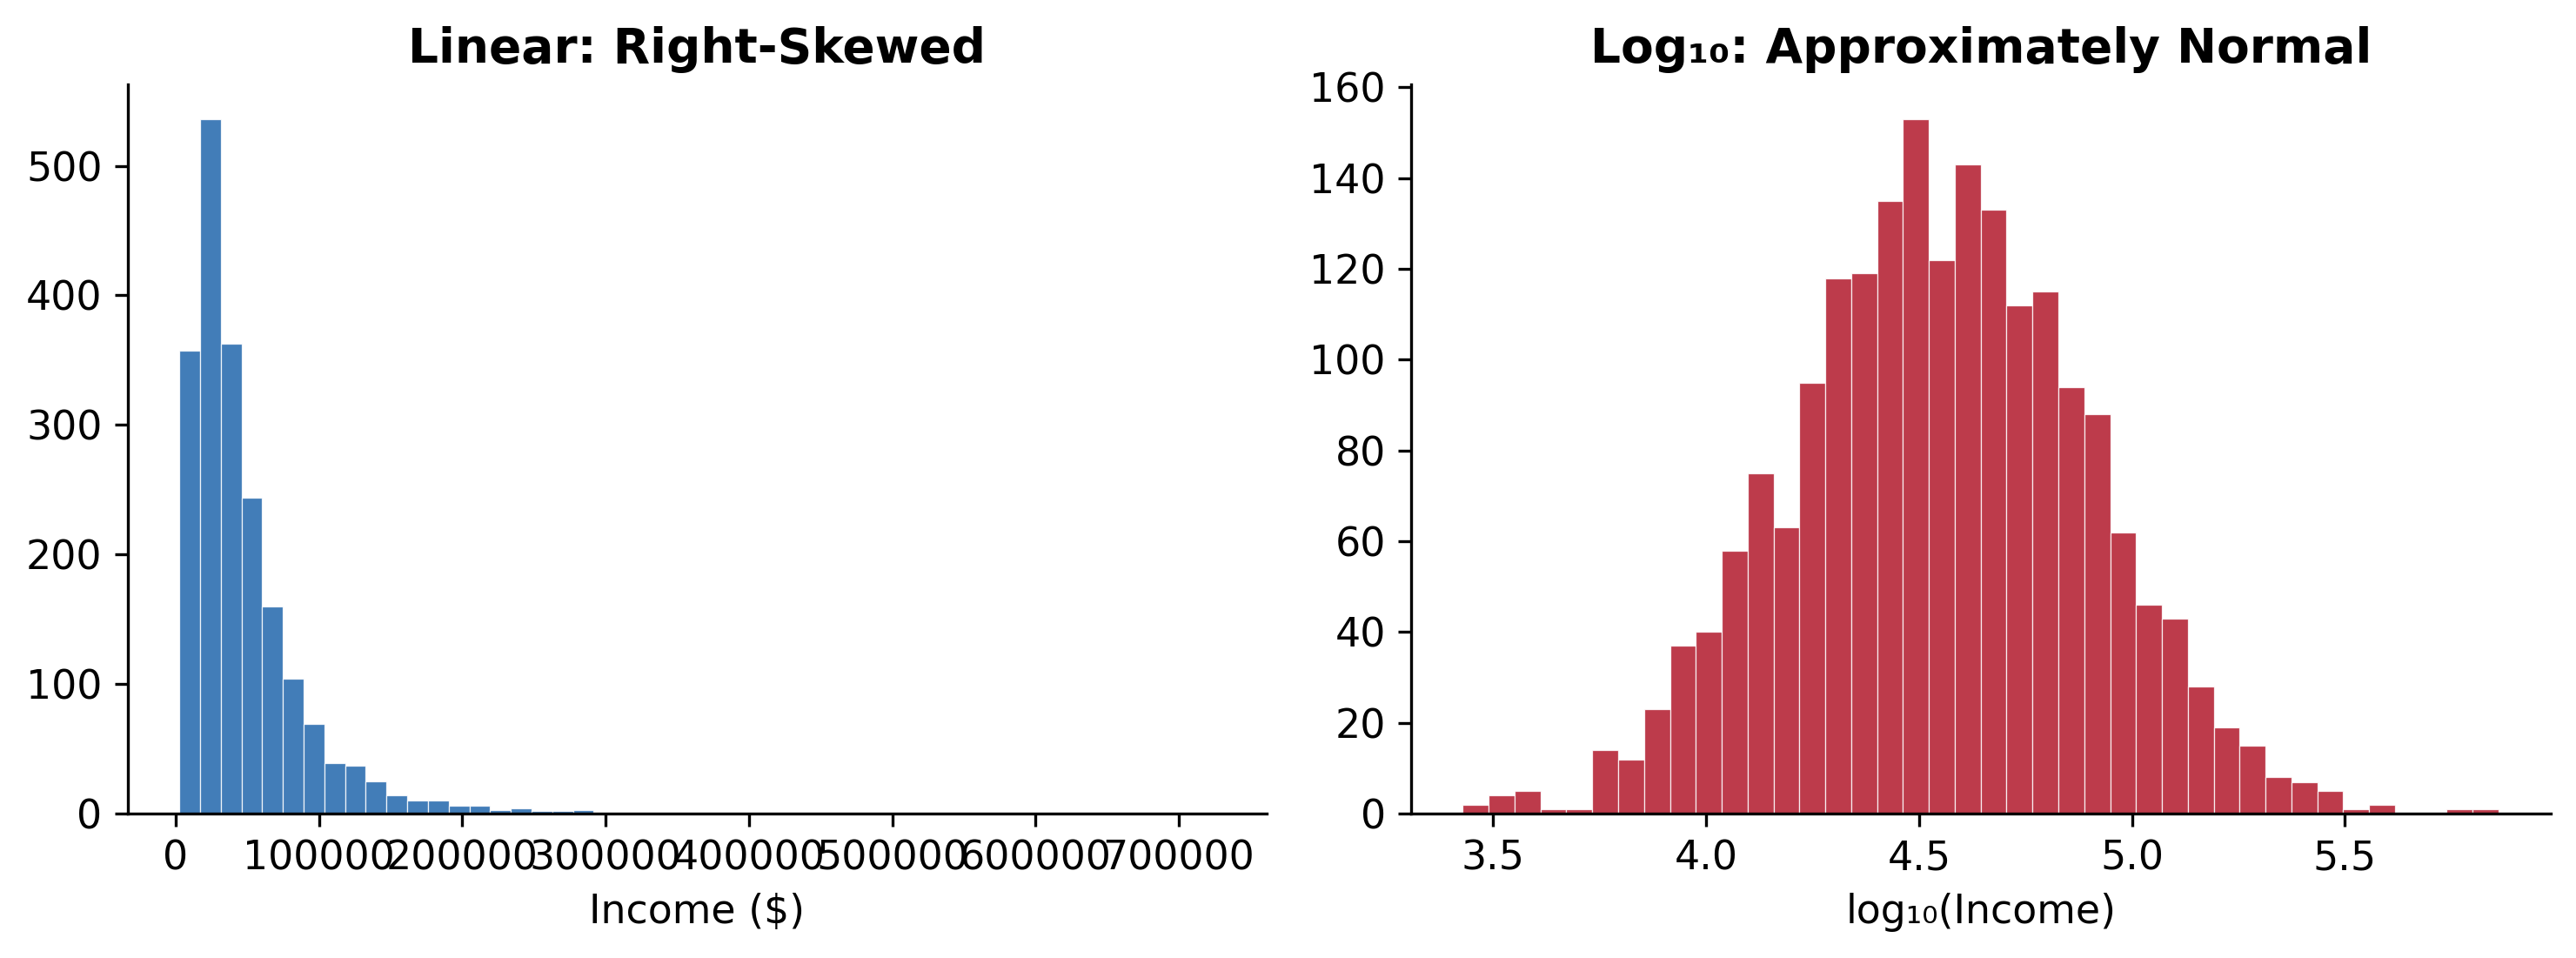
\includegraphics[width=0.88\textwidth]{m1_7_log_hist.png}

\vspace{0.2cm}
\begin{columns}[T]
\begin{column}{0.48\textwidth}
\begin{exampleblock}{Data Insight}
    \scriptsize Income data is classically right-skewed on a linear scale. Log-transform reveals an approximately normal distribution --- the \textbf{lognormal} model.
\end{exampleblock}
\end{column}
\begin{column}{0.48\textwidth}
\begin{alertblock}{Pro-Tip}
    \scriptsize If your histogram is right-skewed, try a log-transformed version. If the log version looks normal, the data is lognormal --- use geometric mean, not arithmetic.
\end{alertblock}
\end{column}
\end{columns}
\end{frame}

% ── 196 ──
\begin{frame}[fragile]{Log Histogram --- Code}\smark{196/300}
\begin{columns}[T]
\begin{column}{0.48\textwidth}
\begin{lstlisting}[style=Rstyle]
# Transform the axis
ggplot(df, aes(income)) +
  geom_histogram(bins = 40,
    fill = "#2166AC") +
  scale_x_log10(
    labels = scales::comma) +
  theme_minimal()

# OR transform the data
ggplot(df, aes(log10(income))) +
  geom_histogram(bins = 40,
    fill = "#B2182B")
\end{lstlisting}
\end{column}
\begin{column}{0.48\textwidth}
\begin{lstlisting}[style=Pystyle]
# Transform axis
plt.hist(income, bins=50)
plt.xscale("log")

# Transform data
plt.hist(np.log10(income),
         bins=40,
         color="#B2182B")
plt.xlabel("log10(Income)")
\end{lstlisting}
\end{column}
\end{columns}
\end{frame}

% ── 197 ──
\begin{frame}{Square Root and Other Transforms}
\smark{197/300}
\begin{columns}[T]
\begin{column}{0.50\textwidth}
\centering
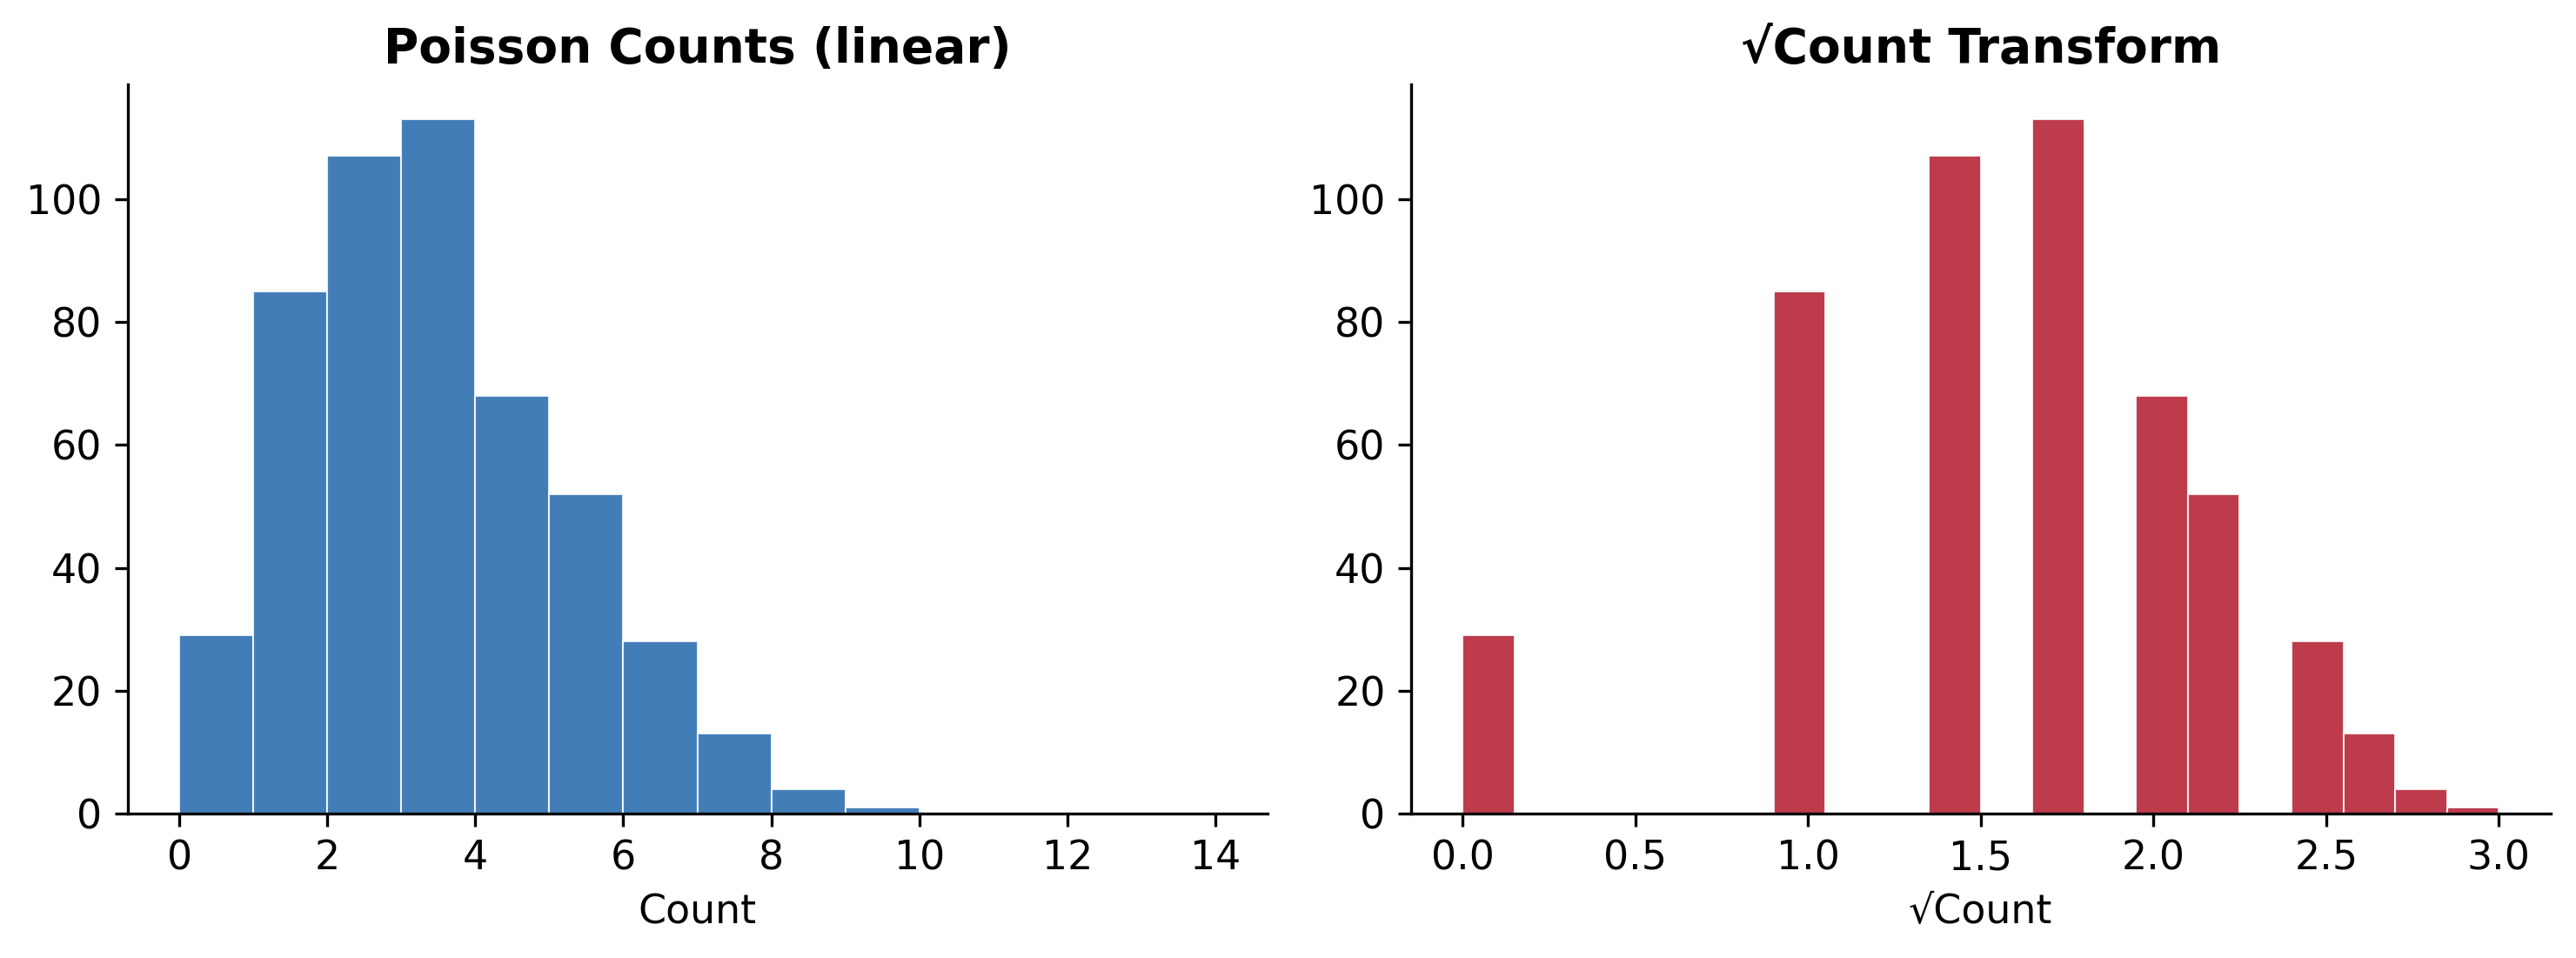
\includegraphics[width=\textwidth]{m1_7_sqrt_transform.png}
\end{column}
\begin{column}{0.47\textwidth}
\centering\small
\begin{tabular}{@{}ll@{}}
    \toprule
    \textbf{Transform} & \textbf{Use Case} \\
    \midrule
    \texttt{log10}  & Orders of magnitude \\
    \texttt{sqrt}   & Count data, Poisson \\
    \texttt{log1p}  & Data with zeros \\
    \texttt{reverse}& Rank data (1 at top) \\
    \texttt{reciprocal} & Rates, per-unit \\
    \bottomrule
\end{tabular}
\vspace{0.2cm}
\begin{alertblock}{Pro-Tip}
    \scriptsize Use \texttt{log1p(x)} = $\log(x+1)$ when data contains zeros. \texttt{log10(0)} = $-\infty$ and will break your plot.
\end{alertblock}
\end{column}
\end{columns}
\end{frame}

% ── 198 ──
\begin{frame}[fragile]{Transforms in ggplot2 --- \Rlang}\smark{198/300}
\begin{columns}[T]
\begin{column}{0.55\textwidth}
\begin{lstlisting}[style=Rstyle]
# Sqrt scale
ggplot(df, aes(x, y)) +
  geom_point() +
  scale_y_sqrt()

# Reverse scale
ggplot(df, aes(team, rank)) +
  geom_point(size = 3) +
  scale_y_reverse() +
  labs(y = "Rank (1 = best)")

# General transform
scale_y_continuous(
  trans = "log1p")
\end{lstlisting}
\end{column}
\begin{column}{0.42\textwidth}
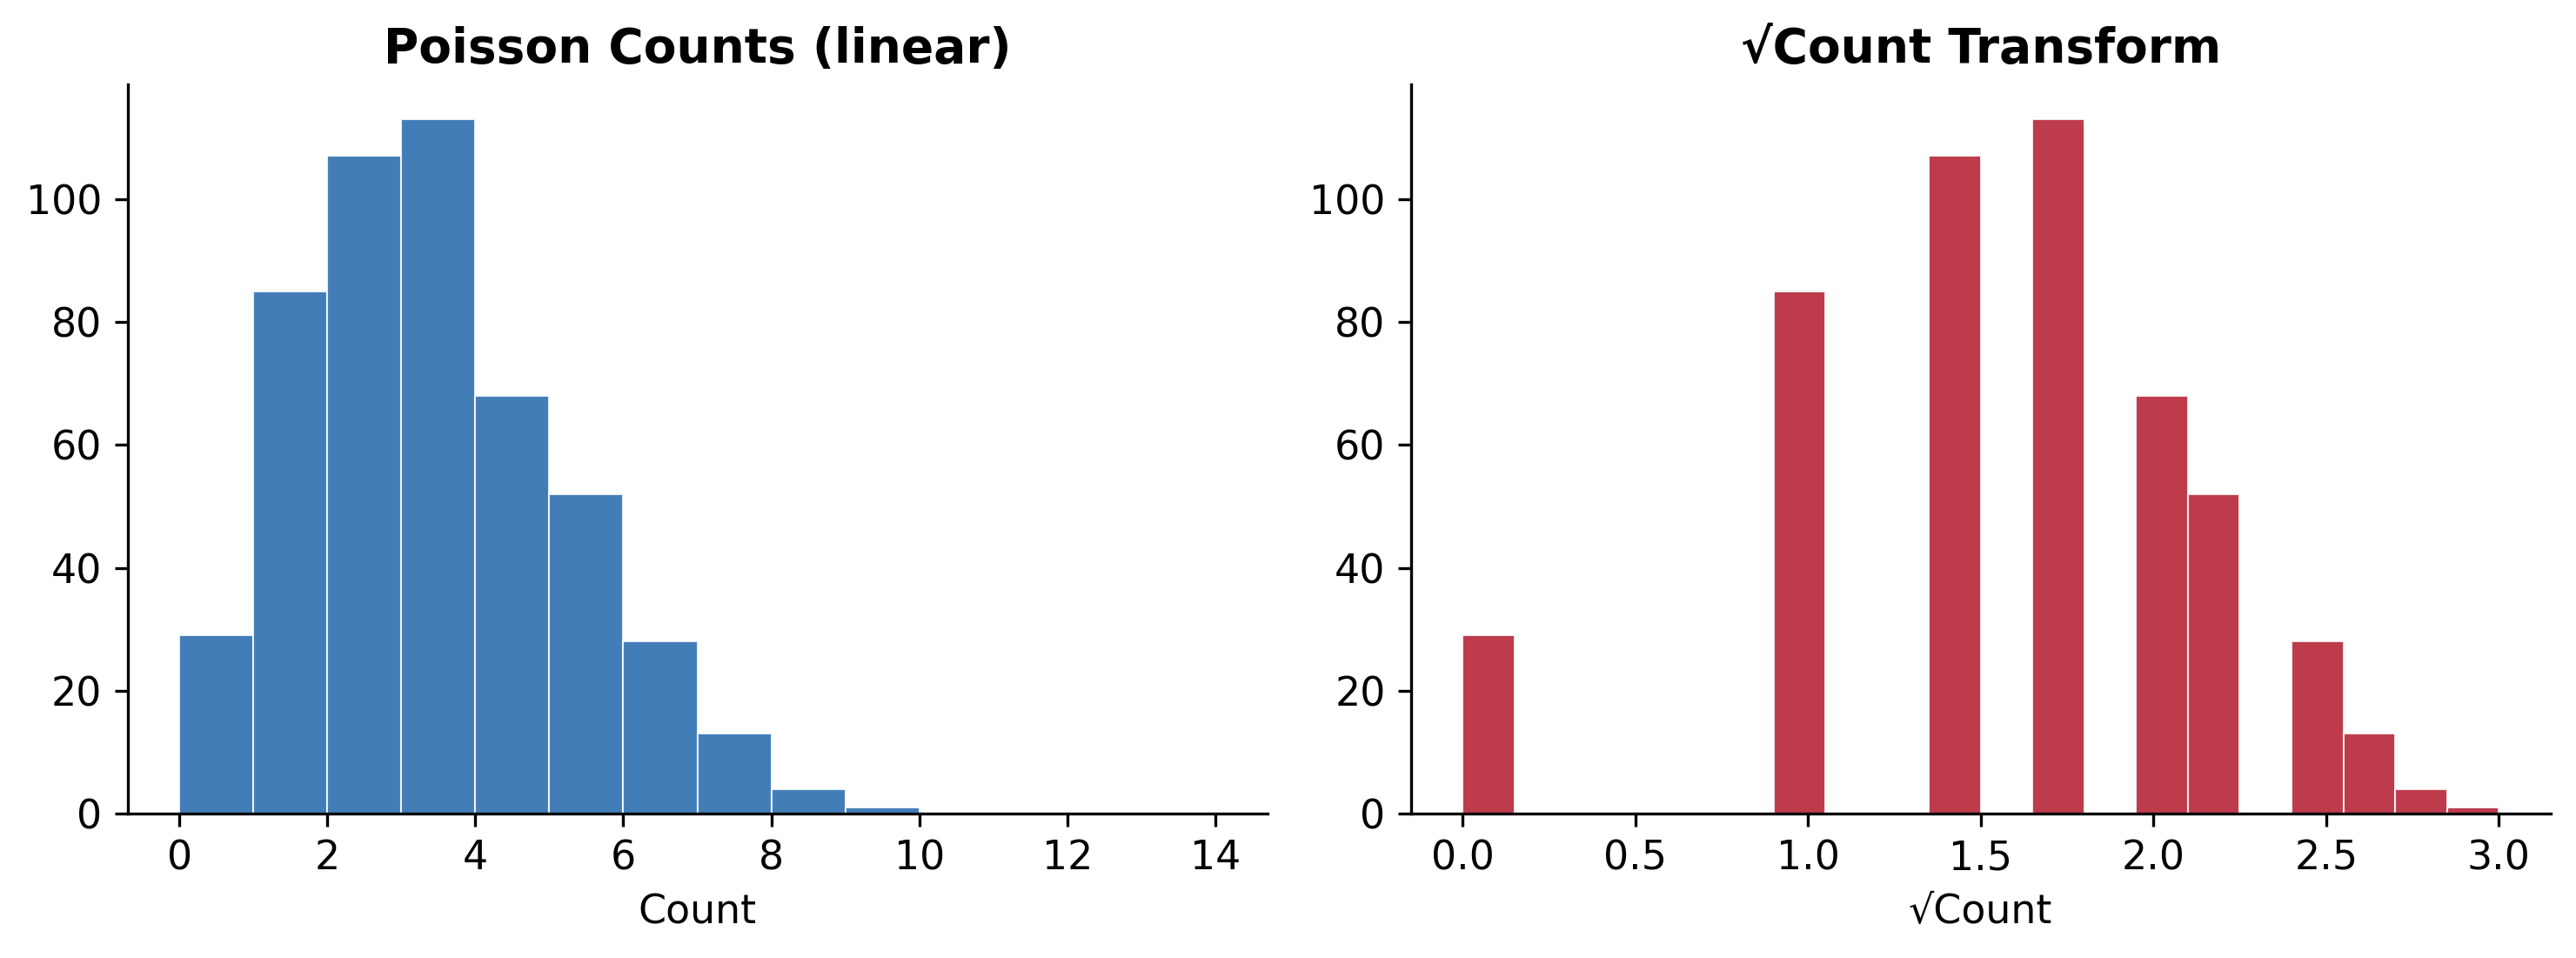
\includegraphics[width=\textwidth]{m1_7_sqrt_transform.png}
\begin{exampleblock}{Data Insight}
    \scriptsize \texttt{scale\_y\_reverse()} is essential for rank data, depth profiles, and any axis where ``up'' means ``less.''
\end{exampleblock}
\end{column}
\end{columns}
\end{frame}

% ── 199 ──
\begin{frame}[fragile]{Transforms --- \Python}\smark{199/300}
\begin{columns}[T]
\begin{column}{0.48\textwidth}
\begin{lstlisting}[style=Pystyle]
# plotnine
(ggplot(df, aes("x","y"))
 + geom_point()
 + scale_y_sqrt())

# Reverse
(ggplot(df, aes("team","rank"))
 + geom_point(size=3)
 + scale_y_reverse())
\end{lstlisting}
\end{column}
\begin{column}{0.48\textwidth}
\begin{lstlisting}[style=Pystyle]
# matplotlib
ax.set_yscale("function",
  functions=(np.sqrt,
             lambda x: x**2))

# Reverse
ax.invert_yaxis()

# symlog (handles zero)
ax.set_yscale("symlog")
\end{lstlisting}
\vspace{0.1cm}
\begin{alertblock}{Pro-Tip}
    \scriptsize matplotlib's \texttt{symlog} handles negative and zero values with a linear region near zero and log regions beyond.
\end{alertblock}
\end{column}
\end{columns}
\end{frame}

% ── 200 ──
\begin{frame}{Reversed Axes}
\smark{200/300}
\centering
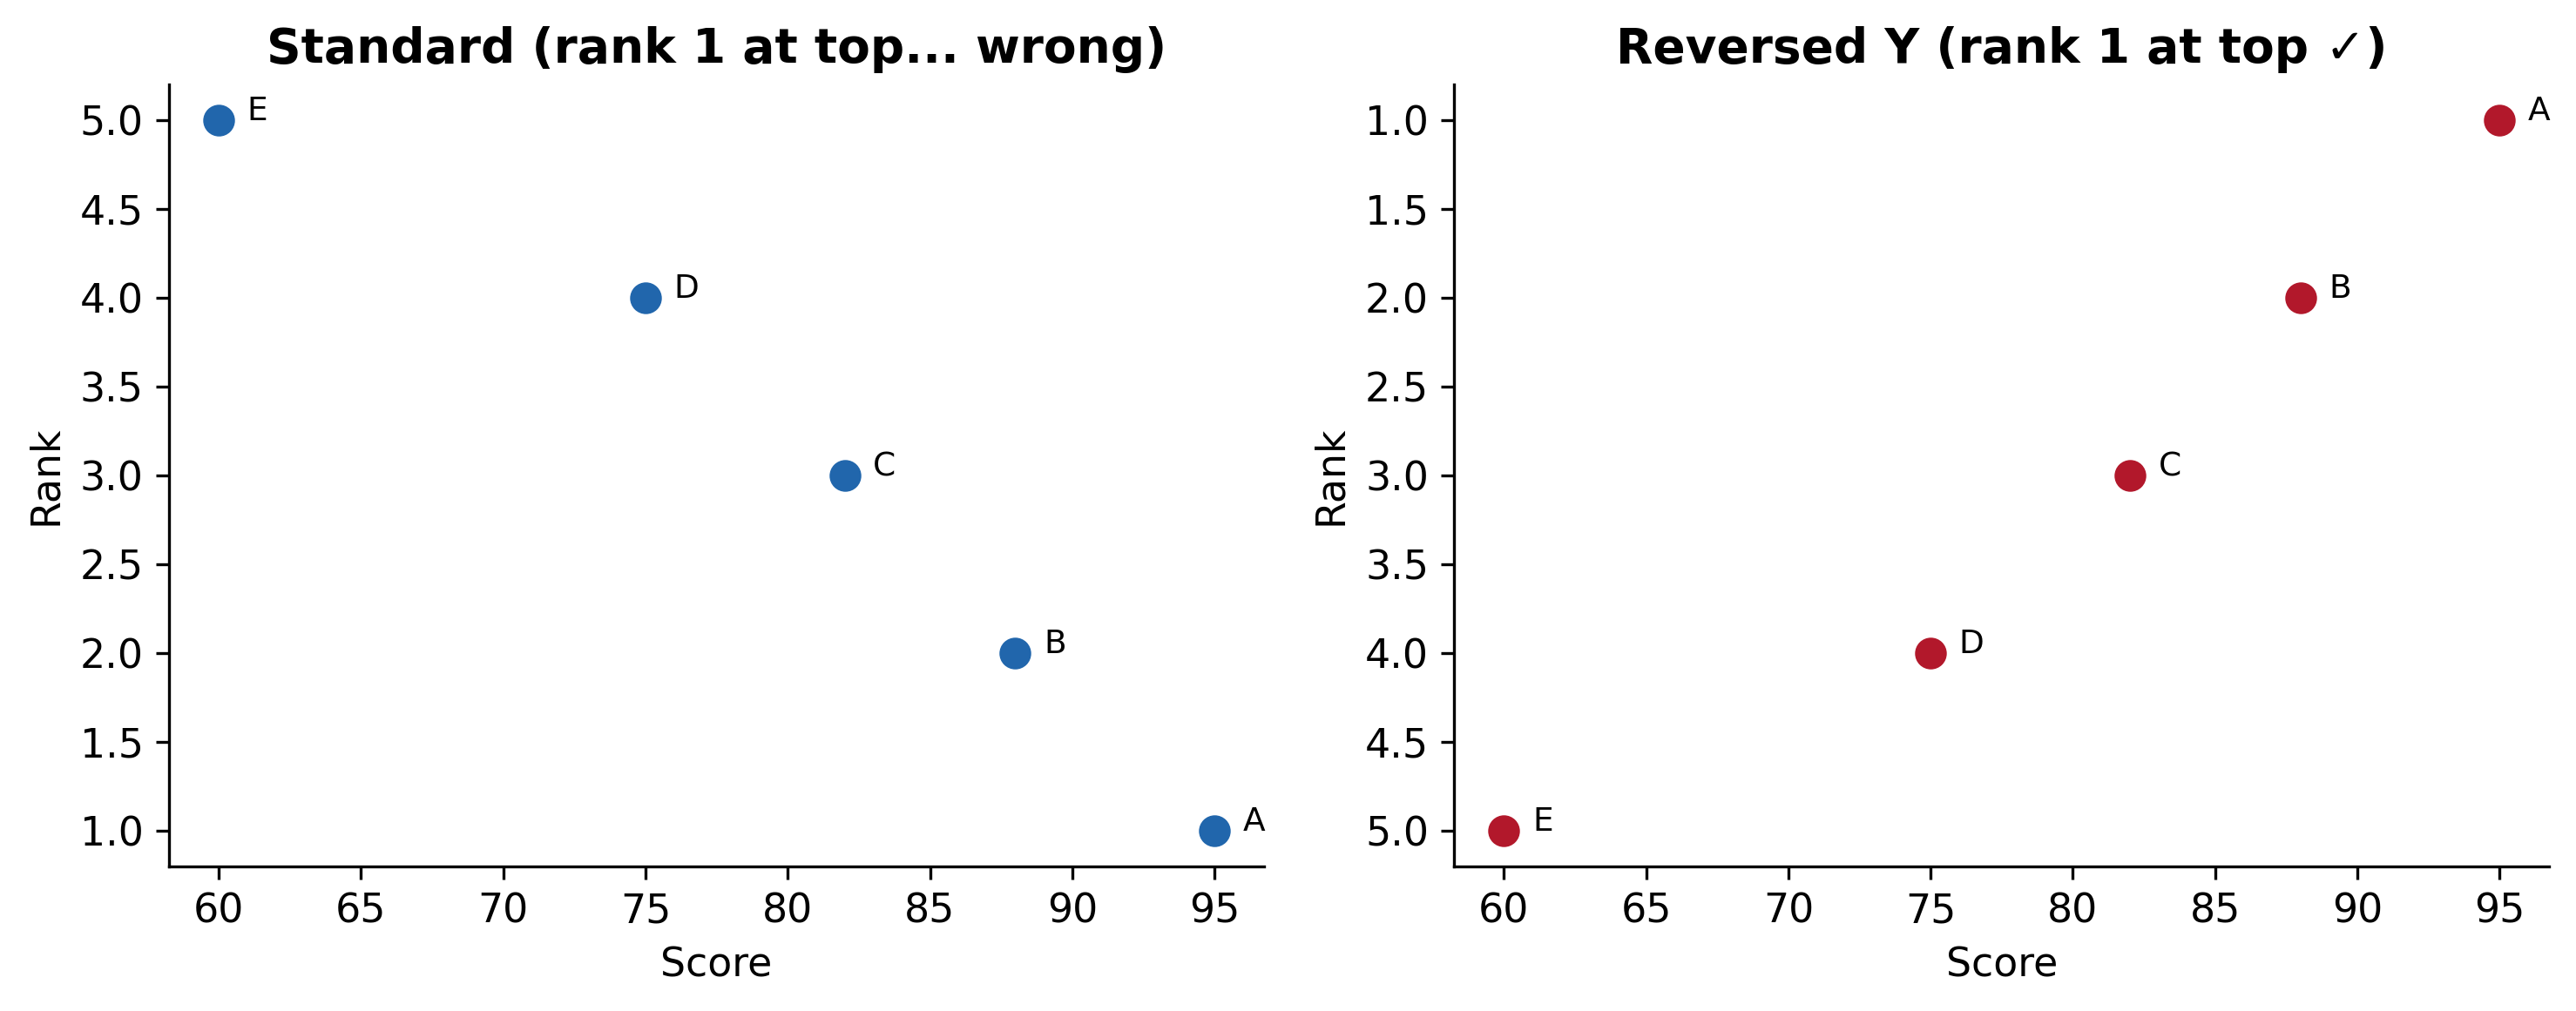
\includegraphics[width=0.88\textwidth]{m1_7_reverse_axis.png}

\vspace{0.2cm}
\begin{exampleblock}{Data Insight}
    \scriptsize Left: rank 1 is at the bottom (counterintuitive). Right: reversed $y$-axis puts rank 1 at the top, matching the reader's expectation. Small fix, large readability gain.
\end{exampleblock}
\end{frame}

% ── 201 ──
\begin{frame}{Aspect Ratio and Banking to 45\textdegree}
\smark{201/300}
\centering
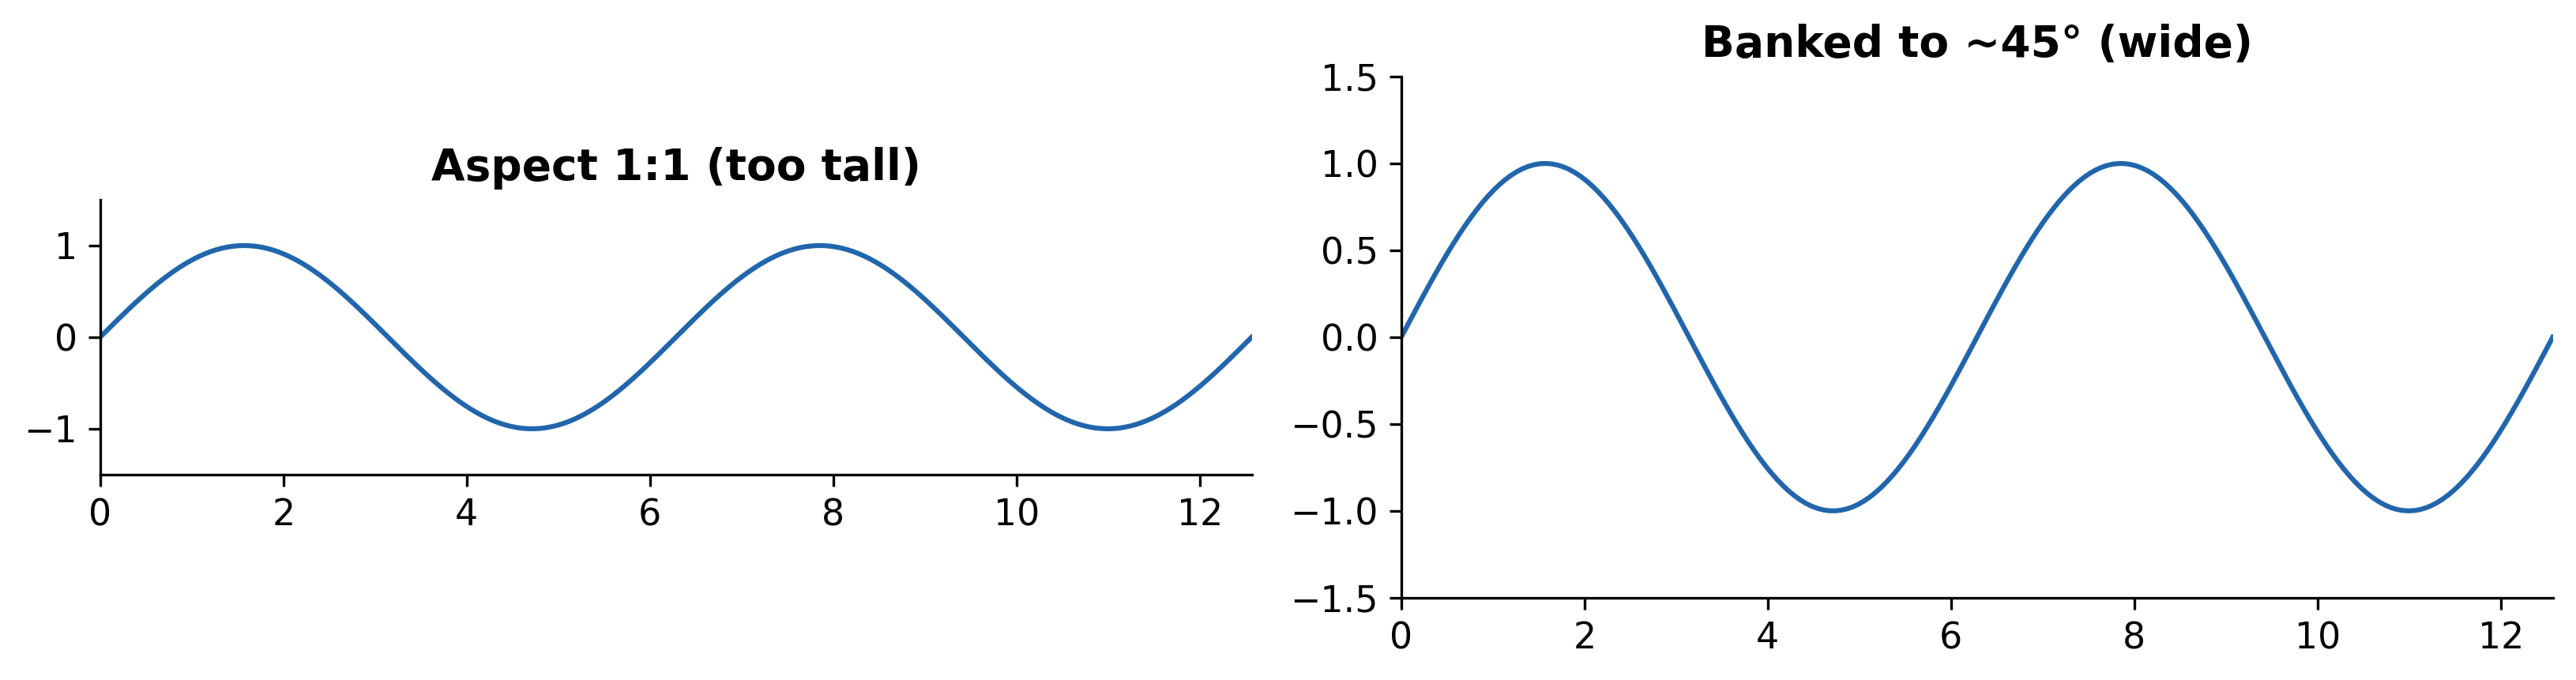
\includegraphics[width=0.88\textwidth]{m1_7_aspect_ratio.png}

\vspace{0.2cm}
\begin{columns}[T]
\begin{column}{0.48\textwidth}
\begin{itemize}
    \item Aspect ratio affects perceived \textbf{slope}
    \item Cleveland (1993): ``bank to 45\textdegree'' --- choose aspect ratio so average slope $\approx 45\textdegree$
    \item Maximizes ability to discriminate rate changes
\end{itemize}
\end{column}
\begin{column}{0.48\textwidth}
\begin{alertblock}{Pro-Tip}
    \scriptsize In ggplot2: \texttt{coord\_fixed(ratio=1)} for equal scaling, or \texttt{theme(aspect.ratio=0.5)} for a specific shape. In matplotlib: \texttt{ax.set\_aspect("equal")} or \texttt{fig.set\_size\_inches(w, h)}.
\end{alertblock}
\end{column}
\end{columns}
\end{frame}

% ── 202 ──
\begin{frame}[fragile]{Aspect Ratio --- Code}\smark{202/300}
\begin{columns}[T]
\begin{column}{0.48\textwidth}
\begin{lstlisting}[style=Rstyle]
# Equal scaling (1:1)
ggplot(df, aes(x, y)) +
  geom_point() +
  coord_fixed(ratio = 1)

# Custom aspect ratio
ggplot(df, aes(date, value)) +
  geom_line() +
  theme(aspect.ratio = 0.4)
# 0.4 = wide and short
\end{lstlisting}
\end{column}
\begin{column}{0.48\textwidth}
\begin{lstlisting}[style=Pystyle]
# matplotlib
fig, ax = plt.subplots(
    figsize=(10, 4))  # wide
ax.set_aspect("equal")
# or
ax.set_box_aspect(0.4)

# plotnine
(ggplot(...) +
 coord_fixed(ratio=1))
\end{lstlisting}
\end{column}
\end{columns}
\vspace{0.2cm}
\begin{exampleblock}{Data Insight}
    \scriptsize For scatterplots where both axes share the same unit (e.g., predicted vs.\ actual), use \texttt{coord\_fixed(ratio=1)} to prevent distortion.
\end{exampleblock}
\end{frame}

% ── 203 ──
\begin{frame}{Discrete Axes and Axis Ordering}
\smark{203/300}
\begin{columns}[T]
\begin{column}{0.50\textwidth}
\begin{itemize}
    \item Categorical $x$ $\to$ discrete axis (equal spacing, no interpolation)
    \item Default order: \textbf{alphabetical} (usually wrong)
    \item Reorder by: value (\texttt{fct\_reorder}), frequency (\texttt{fct\_infreq}), or manual (\texttt{fct\_relevel})
    \item Exception: ordinal categories with intrinsic order (e.g., months, education levels)
\end{itemize}
\end{column}
\begin{column}{0.47\textwidth}
\begin{alertblock}{Pro-Tip}
    \scriptsize The single most impactful fix for most bar charts is \textbf{sorting}. \texttt{fct\_reorder(category, value)} in R; \texttt{sort\_values()} in pandas before plotting.
\end{alertblock}
\vspace{0.2cm}
\begin{exampleblock}{Data Insight}
    \scriptsize Months have intrinsic order (Jan--Dec). Sorting by value would destroy the temporal logic. Always check whether your categories are nominal or ordinal.
\end{exampleblock}
\end{column}
\end{columns}
\end{frame}

% ── 204 ──
\begin{frame}[fragile]{Axis Ordering --- Code}\smark{204/300}
\begin{columns}[T]
\begin{column}{0.48\textwidth}
\begin{lstlisting}[style=Rstyle]
# By value (descending)
ggplot(df,
  aes(fct_reorder(cat, -val),
      val)) +
  geom_col()

# By frequency
ggplot(diamonds,
  aes(fct_infreq(clarity))) +
  geom_bar()

# Manual order
mutate(cut = fct_relevel(cut,
  "Ideal","Premium",
  "Very Good","Good","Fair"))
\end{lstlisting}
\end{column}
\begin{column}{0.48\textwidth}
\begin{lstlisting}[style=Pystyle]
# pandas: sort before plot
df = df.sort_values("val",
    ascending=False)
plt.bar(df["cat"], df["val"])

# Manual order
order = ["Ideal","Premium",
         "Very Good","Good","Fair"]
df["cut"] = pd.Categorical(
    df["cut"],
    categories=order,
    ordered=True)
\end{lstlisting}
\end{column}
\end{columns}
\end{frame}

% ── 205 ──
\begin{frame}{Coordinate System Decision Guide}
\smark{205/300}
\centering\small
\begin{tabular}{@{}lll@{}}
    \toprule
    \textbf{Situation} & \textbf{Coord / Scale} & \textbf{Effect} \\
    \midrule
    Default plot            & \texttt{coord\_cartesian()}    & Orthogonal $x$--$y$ \\
    Horizontal bars         & \texttt{coord\_flip()}         & Swap axes \\
    Pie / Coxcomb           & \texttt{coord\_polar()}        & Wrap around circle \\
    Orders of magnitude     & \texttt{scale\_x\_log10()}     & Log spacing, linear labels \\
    Zoom without data loss  & \texttt{coord\_cartesian(xlim)}& Viewport clip \\
    Equal physical units    & \texttt{coord\_fixed(ratio=1)} & 1:1 aspect \\
    Map projection          & \texttt{coord\_sf()}           & Module 6 (geospatial) \\
    Rank data (1 at top)    & \texttt{scale\_y\_reverse()}   & Invert $y$ \\
    Count data / Poisson    & \texttt{scale\_y\_sqrt()}      & Stabilize variance \\
    \bottomrule
\end{tabular}
\end{frame}

% ── 206 ──
\begin{frame}[fragile]{Combining Transforms with Facets}\smark{206/300}
\begin{columns}[T]
\begin{column}{0.48\textwidth}
\begin{lstlisting}[style=Rstyle]
# Faceted + log y
ggplot(penguins,
  aes(bill_length_mm,
      body_mass_g,
      color = species)) +
  geom_point(alpha = 0.7) +
  facet_wrap(~island) +
  scale_y_log10() +
  theme_minimal()
\end{lstlisting}
\end{column}
\begin{column}{0.48\textwidth}
\begin{lstlisting}[style=Pystyle]
(ggplot(penguins,
   aes("bill_length_mm",
       "body_mass_g",
       color="species"))
 + geom_point(alpha=0.7)
 + facet_wrap("~island")
 + scale_y_log10())
\end{lstlisting}
\vspace{0.2cm}
\begin{exampleblock}{Data Insight}
    \scriptsize Coords and scales apply \textbf{uniformly across all facets}. You cannot have log scale in one panel and linear in another (by design --- it would break cross-panel comparison).
\end{exampleblock}
\end{column}
\end{columns}
\end{frame}

% ── 207 ──
\begin{frame}{Date and Time Axes}
\smark{207/300}
\begin{columns}[T]
\begin{column}{0.50\textwidth}
\begin{itemize}
    \item Dates are continuous --- handled by \texttt{scale\_x\_date()}
    \item Control breaks: \texttt{date\_breaks = "3 months"}
    \item Control labels: \texttt{date\_labels = "\%b \%Y"}
    \item Datetime: \texttt{scale\_x\_datetime()} with finer breaks
    \item Module 4 covers temporal data in depth
\end{itemize}
\end{column}
\begin{column}{0.47\textwidth}
\begin{alertblock}{Pro-Tip}
    \scriptsize Date axes often need manual break/label control. The default may show every day (unreadable) or every decade (too sparse). Set \texttt{date\_breaks} and \texttt{date\_labels} explicitly.
\end{alertblock}
\vspace{0.2cm}
\begin{exampleblock}{Data Insight}
    \scriptsize In Python: \texttt{matplotlib.dates.DateFormatter("\%b \%Y")} and \texttt{mdates.MonthLocator(interval=3)} achieve the same.
\end{exampleblock}
\end{column}
\end{columns}
\end{frame}

% ── 208 ──
\begin{frame}[fragile]{Date Axes --- Code}\smark{208/300}
\begin{columns}[T]
\begin{column}{0.48\textwidth}
\begin{lstlisting}[style=Rstyle]
ggplot(economics,
  aes(date, unemploy)) +
  geom_line(color="#2166AC") +
  scale_x_date(
    date_breaks = "5 years",
    date_labels = "%Y") +
  theme_minimal()
\end{lstlisting}
\end{column}
\begin{column}{0.48\textwidth}
\begin{lstlisting}[style=Pystyle]
import matplotlib.dates as mdates

ax.plot(dates, values)
ax.xaxis.set_major_locator(
    mdates.YearLocator(5))
ax.xaxis.set_major_formatter(
    mdates.DateFormatter("%Y"))
plt.xticks(rotation=45)
\end{lstlisting}
\end{column}
\end{columns}
\end{frame}

% ── 209 ──
\begin{frame}{Module 1.7 --- Key Takeaways}\smark{209/300}
\begin{enumerate}
    \item \textbf{Zoom with \texttt{coord\_cartesian}}, not scale limits --- preserves stat layers.
    \item \textbf{\texttt{coord\_flip}} for horizontal bars and long labels.
    \item \textbf{Pie = bar + \texttt{coord\_polar("y")}.} The grammar makes this explicit.
    \item \textbf{Log scale} when data spans orders of magnitude. Use \texttt{scale\_x\_log10()}.
    \item \textbf{Log axis vs.\ log data}: axis keeps original labels; data changes units.
    \item \textbf{Aspect ratio} affects slope perception. Bank to 45\textdegree\ for time series.
\end{enumerate}
\end{frame}

% ── 210 ──
\begin{frame}{}\smark{210/300}
\centering\vspace{1.5cm}
{\Large\textbf{Module 1.7 Complete}}\\[0.5cm]
You now control coordinate systems --- Cartesian, polar, flipped, log-transformed, reversed --- and understand the critical distinction between viewport zooming and data filtering.\\[0.5cm]
\textbf{Next:} Module 1.8 --- Themes, Typography, and Visual Identity.
\end{frame}

% ═══════════════════════════════════════════════════════
%  MODULE 1.8 — Themes, Typography, and Visual Identity
% ═══════════════════════════════════════════════════════
\section{Module 1.8 --- Themes, Typography, and Visual Identity}

% ── 211 ──
\begin{frame}{Module 1.8 --- Roadmap}\smark{211/300}
\begin{enumerate}
    \item Built-in themes: minimal, bw, classic, void
    \item The \texttt{theme()} element anatomy
    \item Gridlines, backgrounds, and borders
    \item Legend positioning and customization
    \item Font selection: sans-serif vs.\ serif vs.\ mono
    \item Dark themes for presentations
    \item Building a custom brand theme
    \item Before/after: the theme makeover
\end{enumerate}
\end{frame}

% ── 212 ──
\begin{frame}{Why Themes Matter}
\smark{212/300}
\begin{columns}[T]
\begin{column}{0.50\textwidth}
\begin{itemize}
    \item Themes control \textbf{everything that is not data}
    \item The same data + geom + aes can look professional or amateurish depending on theme
    \item A consistent theme across figures creates \textbf{visual identity}
    \item Journals, companies, and courses each have style requirements
\end{itemize}
\end{column}
\begin{column}{0.47\textwidth}
\begin{exampleblock}{Data Insight}
    \scriptsize Themes are the \textbf{last layer} applied. They never change data mappings, statistical computations, or geometric shapes --- only visual styling. This orthogonality is by design.
\end{exampleblock}
\vspace{0.2cm}
\begin{alertblock}{Pro-Tip}
    \scriptsize Set your theme \textbf{once} at the top of a script with \texttt{theme\_set(theme\_minimal())}. Every subsequent plot inherits it.
\end{alertblock}
\end{column}
\end{columns}
\end{frame}

% ── 213 ──
\begin{frame}{Four Built-In Themes}
\smark{213/300}
\centering
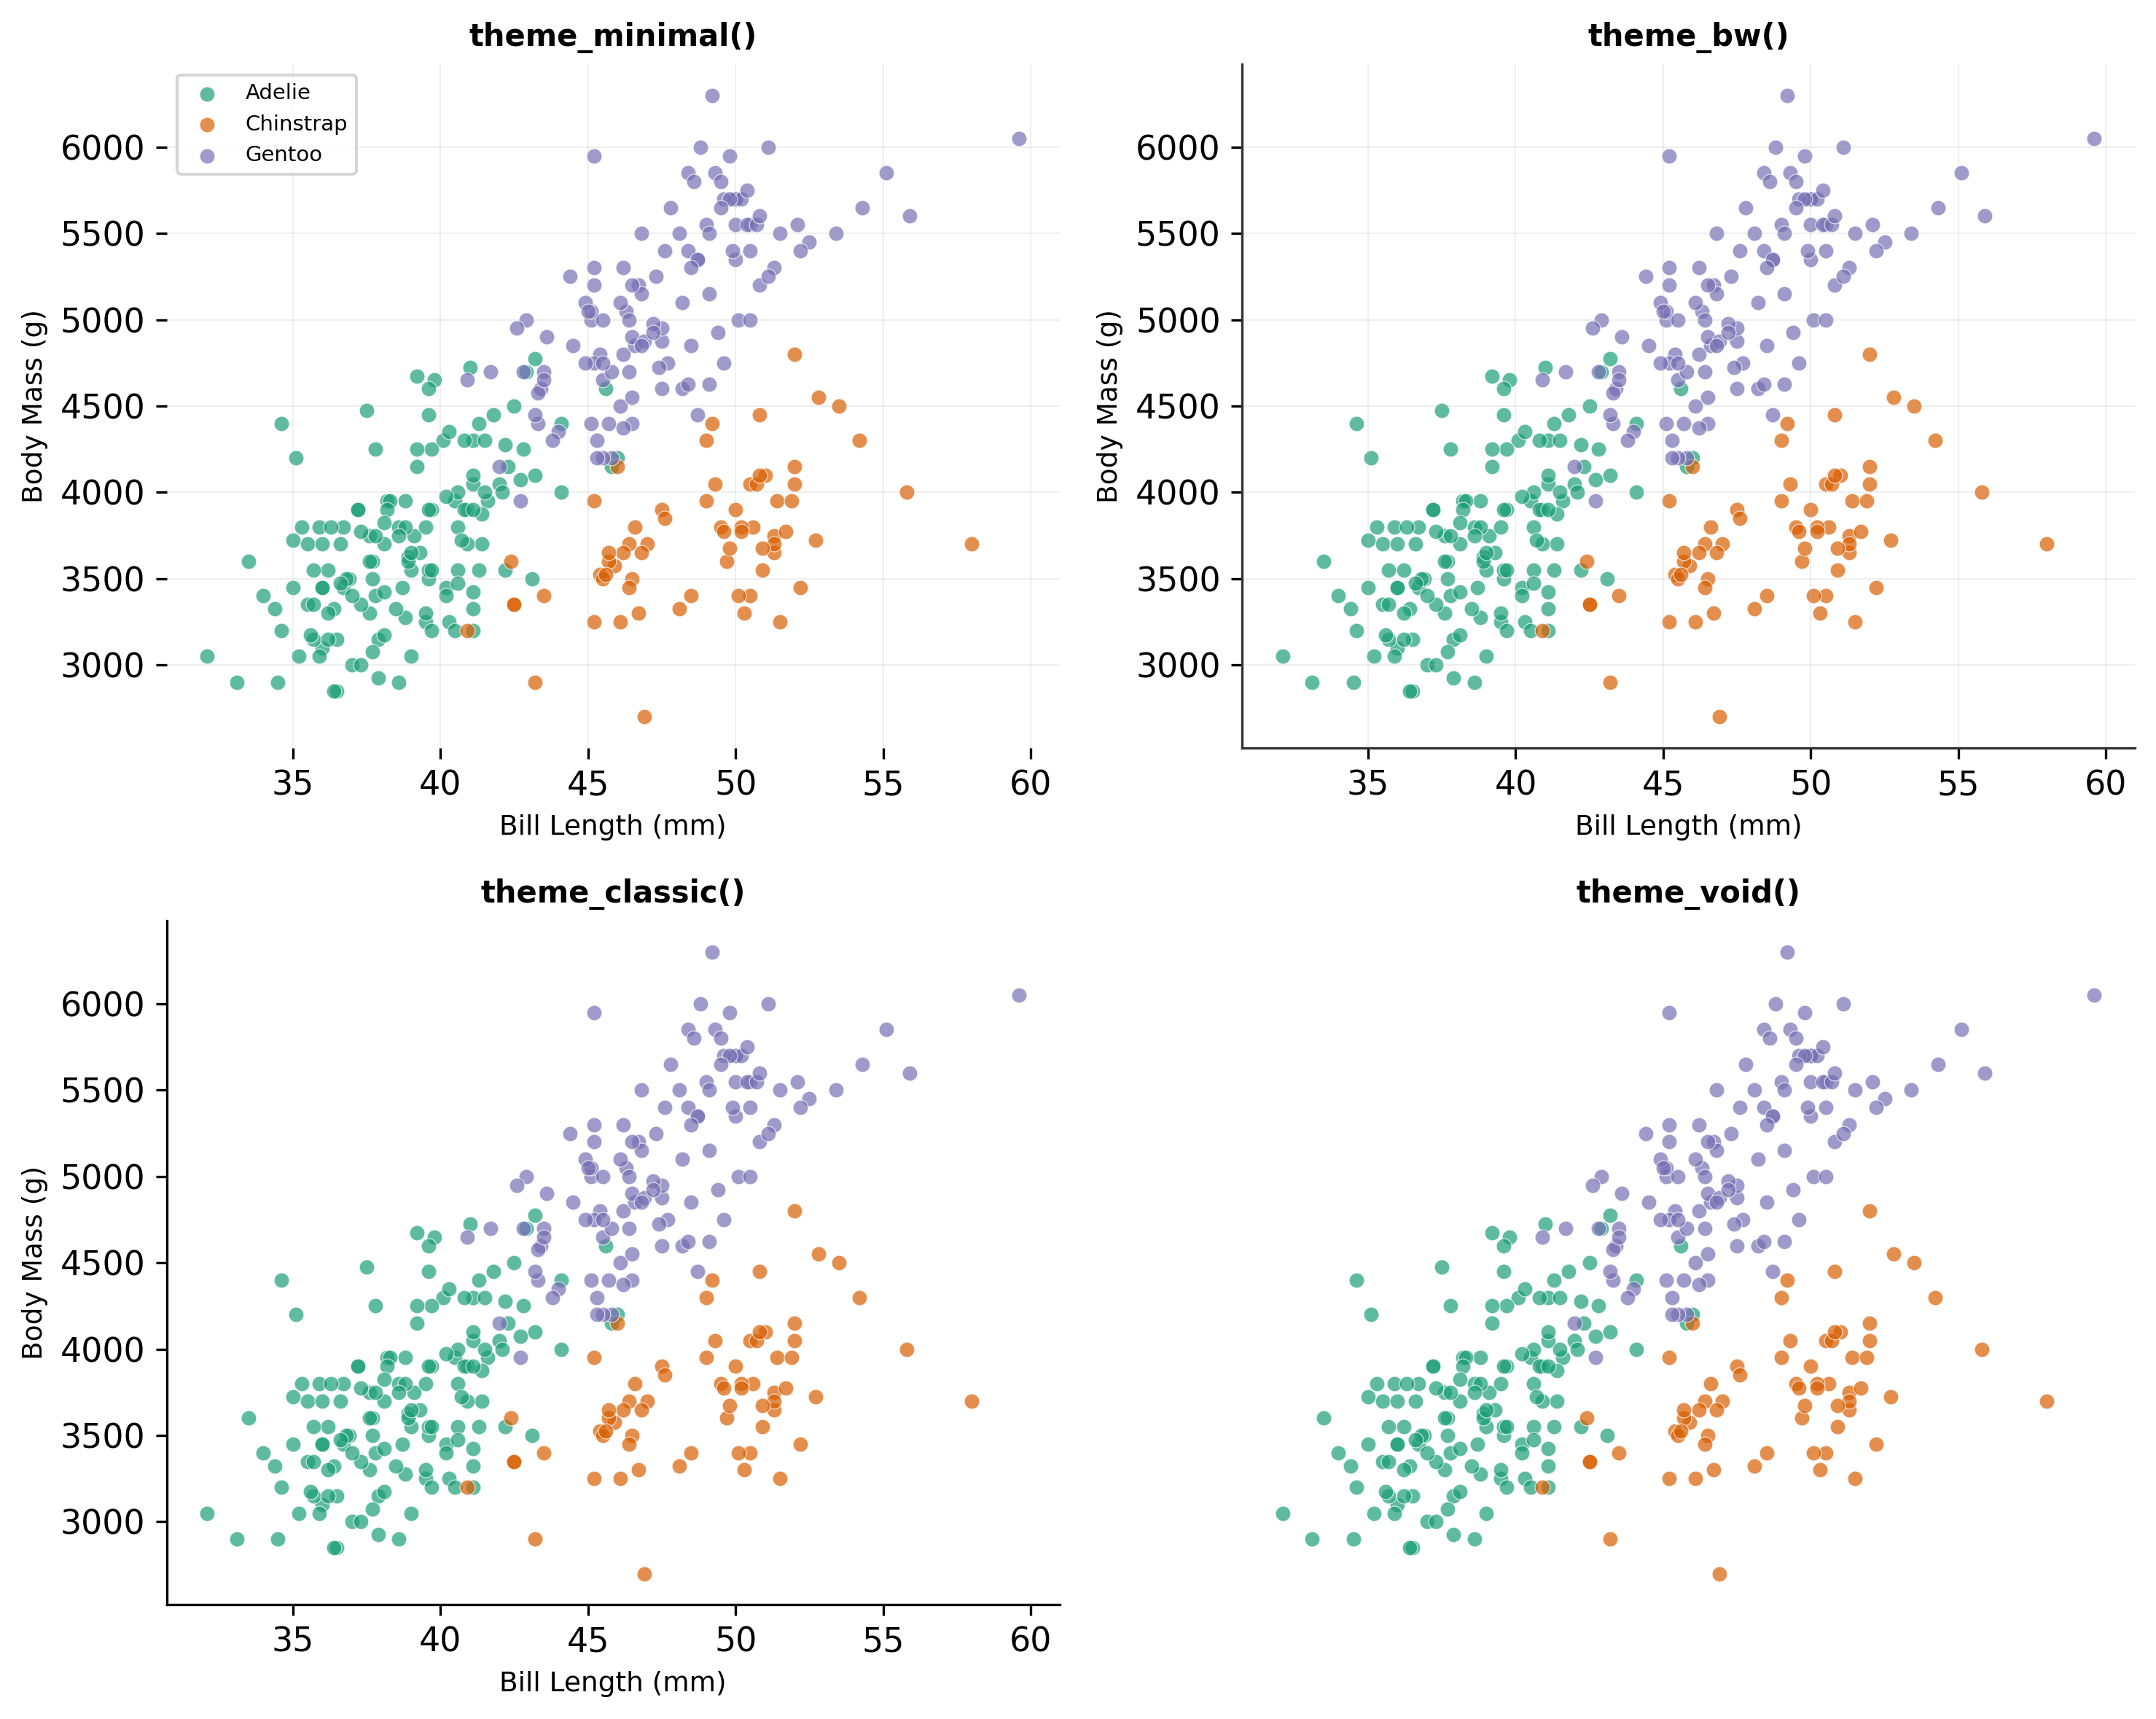
\includegraphics[width=0.85\textwidth]{m1_8_four_themes.png}

\vspace{0.2cm}
\begin{exampleblock}{Data Insight}
    \scriptsize \texttt{theme\_minimal()} is the most popular starting point: no panel border, light gridlines, clean. \texttt{theme\_void()} strips everything --- used for maps, diagrams, and pie charts.
\end{exampleblock}
\end{frame}

% ── 214 ──
\begin{frame}[fragile]{Built-In Themes --- \Rlang}\smark{214/300}
\begin{columns}[T]
\begin{column}{0.55\textwidth}
\begin{lstlisting}[style=Rstyle]
# Apply to a single plot
ggplot(penguins, aes(bill_length_mm,
    body_mass_g, color=species)) +
  geom_point() +
  theme_minimal()

# Set globally (all plots)
theme_set(theme_minimal(
  base_size = 12))

# Other built-ins:
# theme_bw()      gray bg, border
# theme_classic()  axes only, no grid
# theme_void()     nothing
# theme_light()    light gray bg
# theme_dark()     dark bg
\end{lstlisting}
\end{column}
\begin{column}{0.42\textwidth}
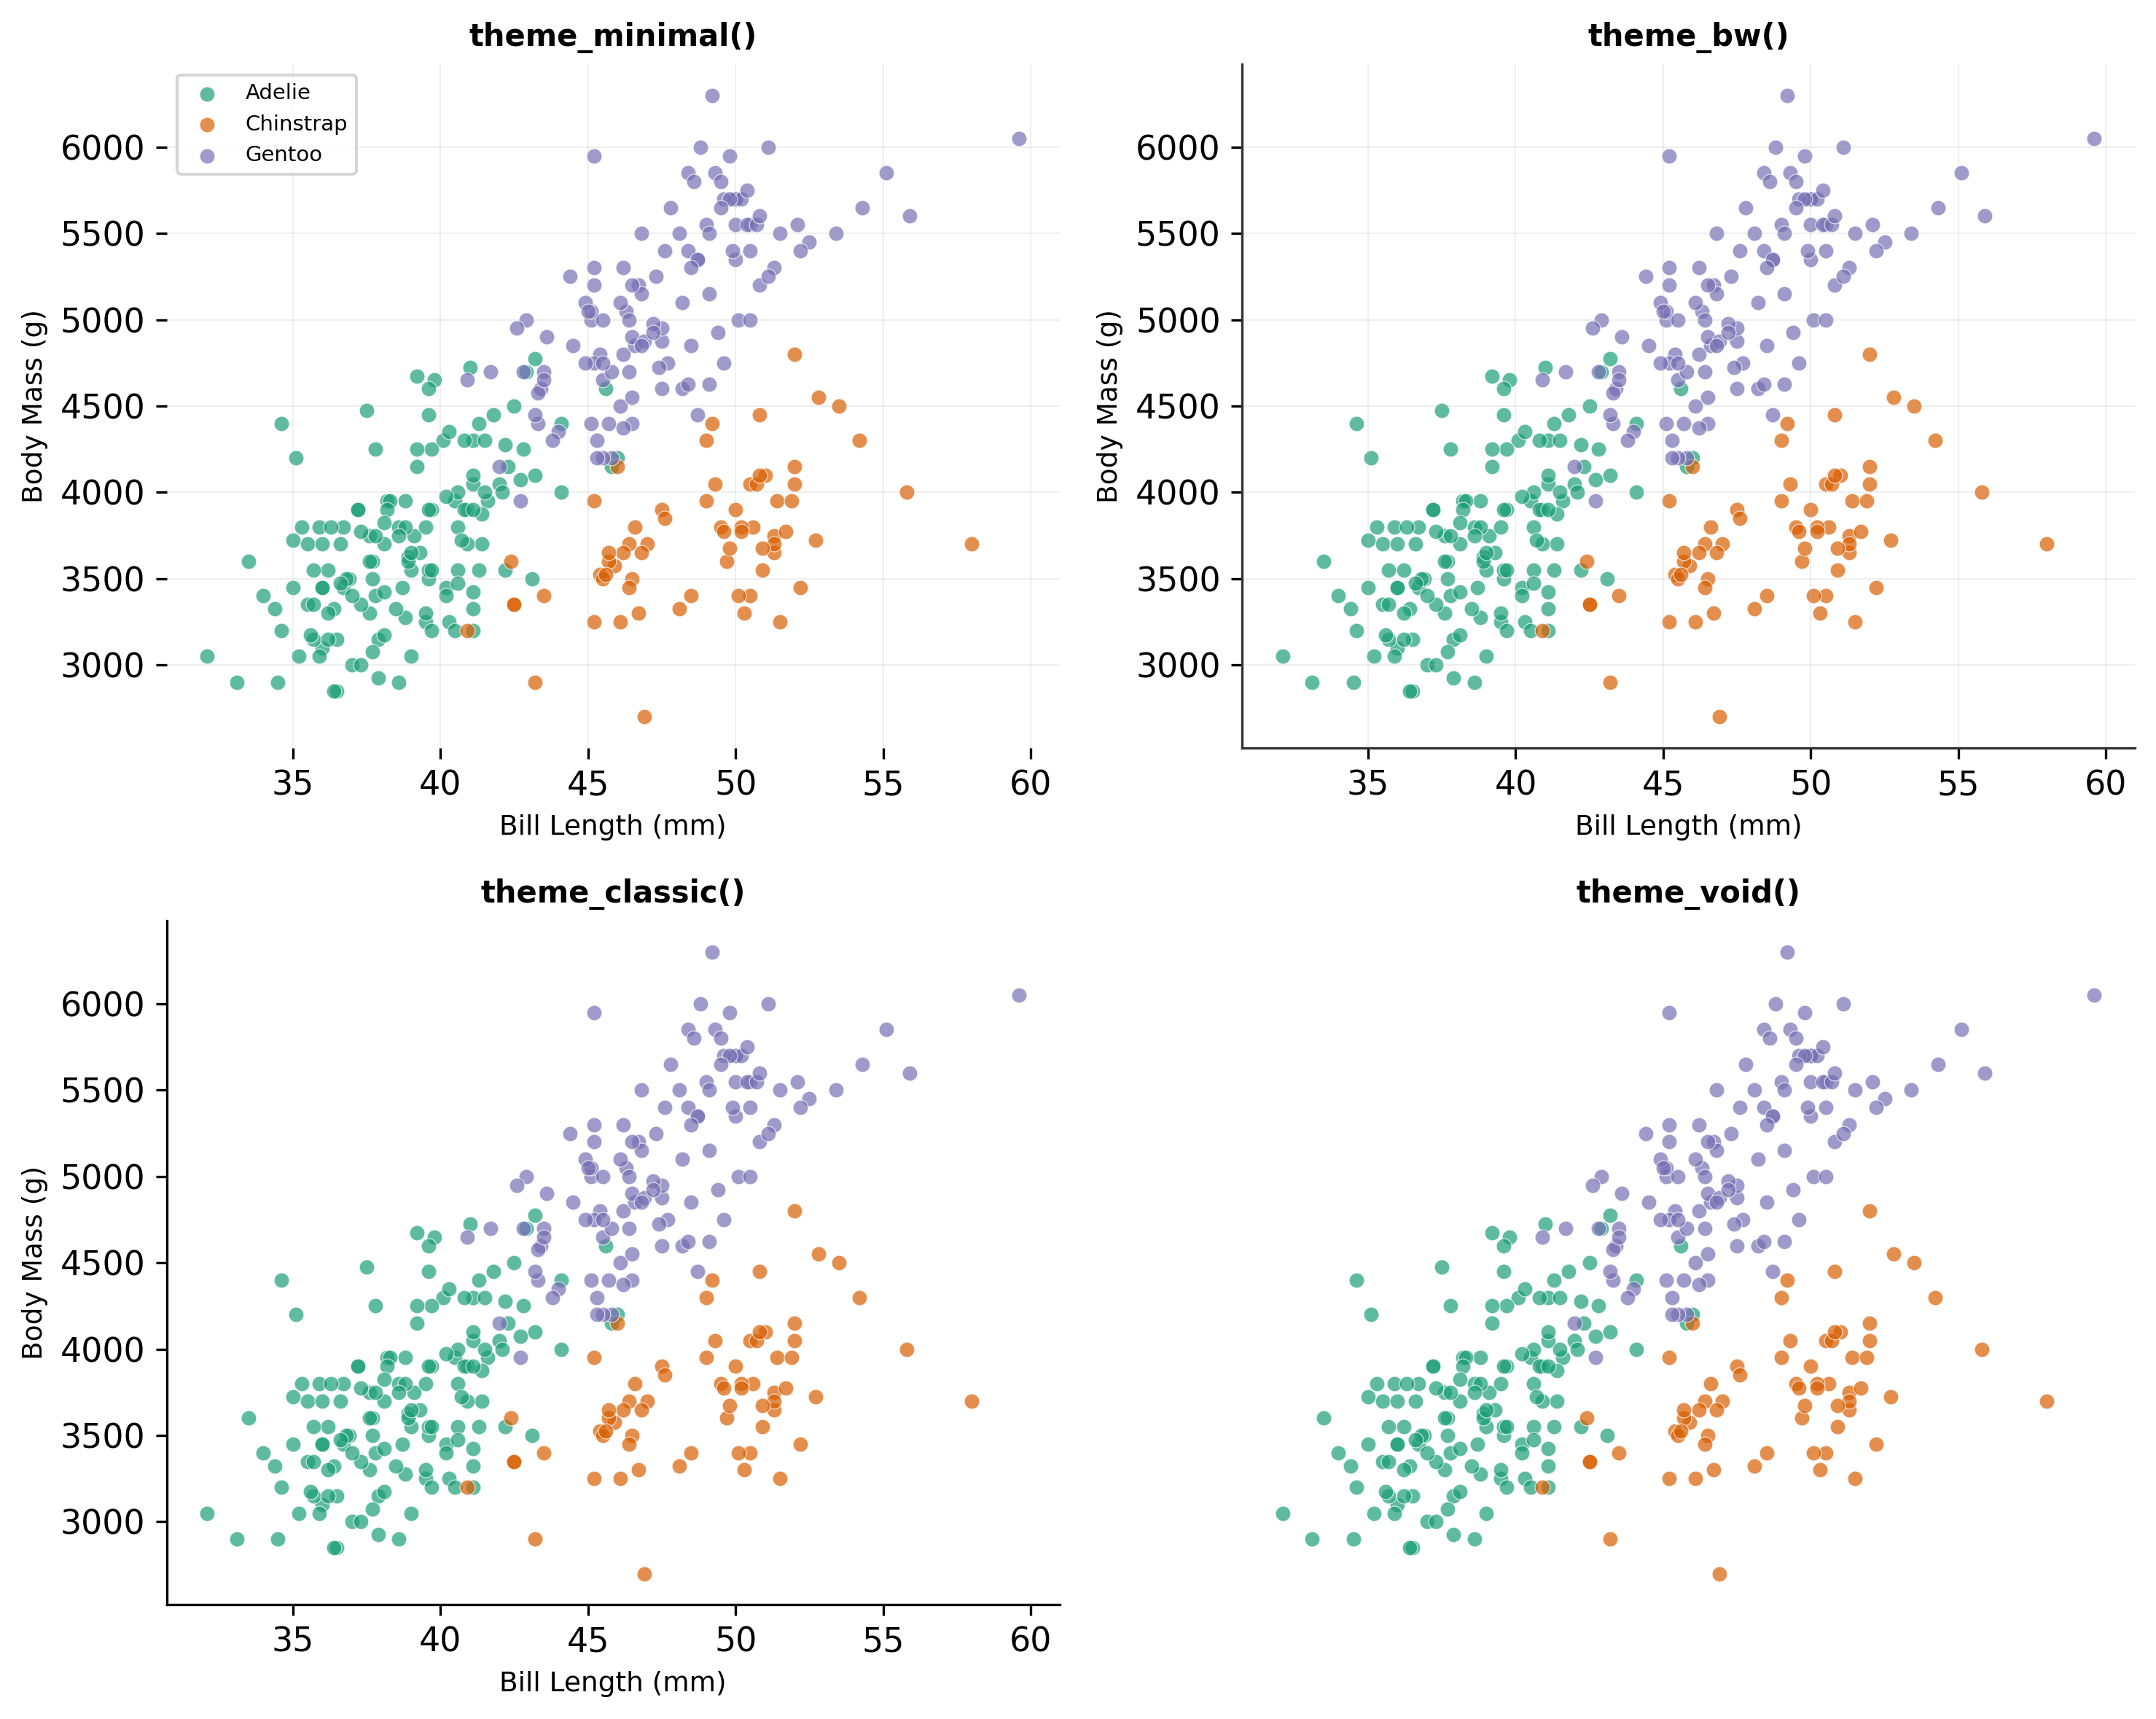
\includegraphics[width=\textwidth]{m1_8_four_themes.png}
\begin{alertblock}{Pro-Tip}
    \scriptsize \texttt{base\_size} controls the root font size. All other text elements scale relative to it. Set it to 12 for papers, 16 for slides.
\end{alertblock}
\end{column}
\end{columns}
\end{frame}

% ── 215 ──
\begin{frame}[fragile]{Built-In Themes --- \Python}\smark{215/300}
\begin{columns}[T]
\begin{column}{0.48\textwidth}
\begin{lstlisting}[style=Pystyle]
# plotnine: identical syntax
(ggplot(...) + theme_minimal())
(ggplot(...) + theme_bw())
(ggplot(...) + theme_void())

# Set globally
from plotnine import theme_set
theme_set(theme_minimal())
\end{lstlisting}
\end{column}
\begin{column}{0.48\textwidth}
\begin{lstlisting}[style=Pystyle]
# matplotlib rcParams
plt.style.use("seaborn-v0_8-whitegrid")
# or
plt.rcParams.update({
    "axes.facecolor": "white",
    "axes.grid": True,
    "grid.alpha": 0.2})

# seaborn
sns.set_style("whitegrid")
sns.set_context("talk") # for slides
\end{lstlisting}
\end{column}
\end{columns}
\vspace{0.1cm}
\begin{exampleblock}{Data Insight}
    \scriptsize seaborn's \texttt{set\_context("talk")} scales fonts and elements up for presentations, similar to ggplot2's \texttt{base\_size=16}.
\end{exampleblock}
\end{frame}

% ── 216 ──
\begin{frame}{The \texttt{theme()} Element Anatomy}
\smark{216/300}
\centering
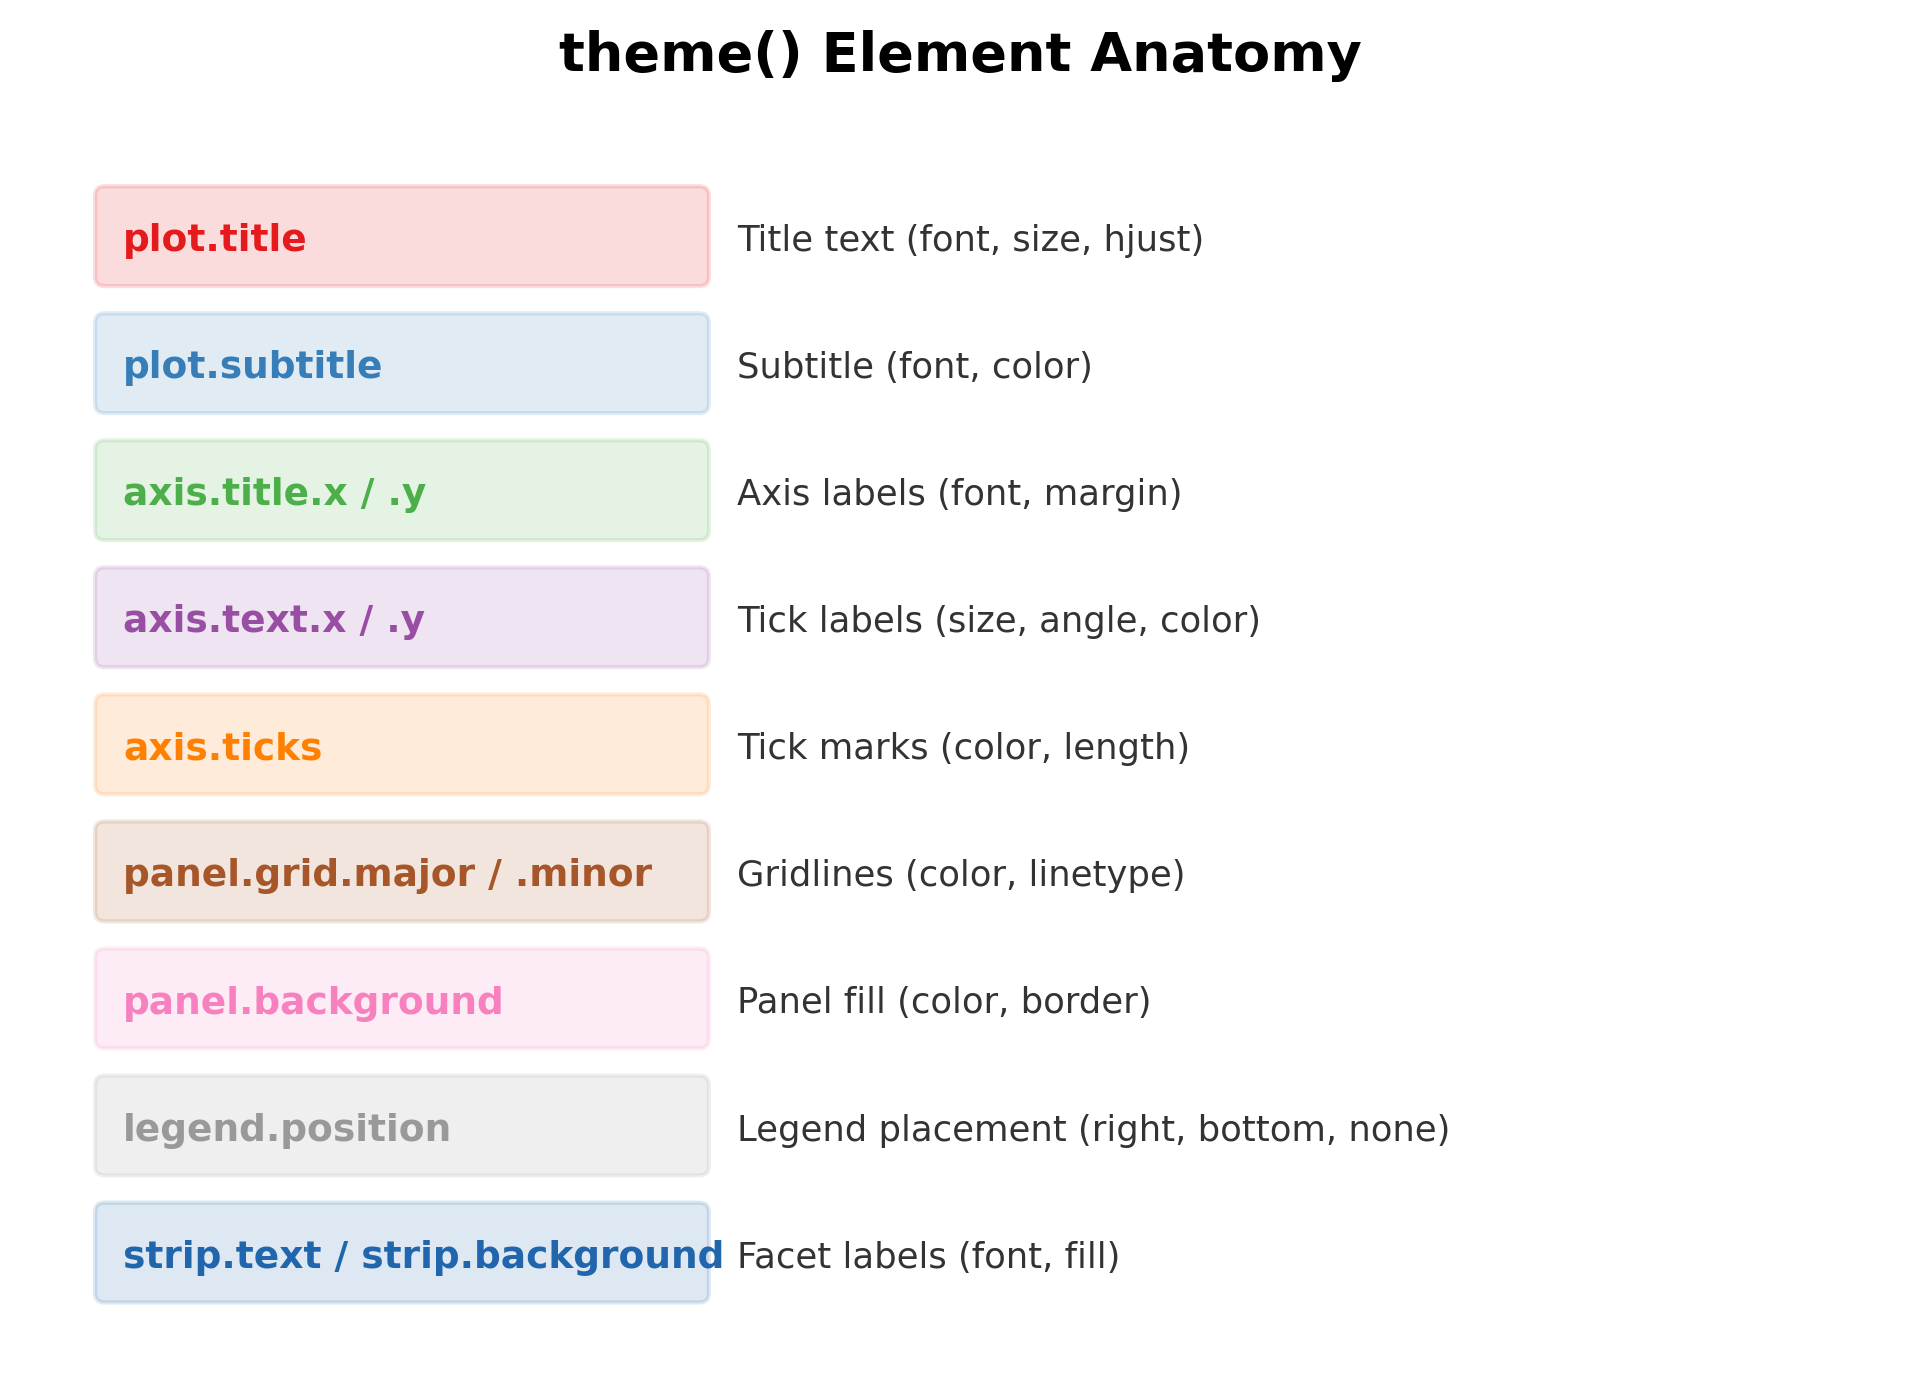
\includegraphics[width=0.72\textwidth]{m1_8_theme_anatomy.png}

\vspace{0.2cm}
\begin{alertblock}{Pro-Tip}
    \scriptsize Every element is set with one of four functions: \texttt{element\_text()}, \texttt{element\_line()}, \texttt{element\_rect()}, or \texttt{element\_blank()} (to remove it entirely).
\end{alertblock}
\end{frame}

% ── 217 ──
\begin{frame}[fragile]{Customizing \texttt{theme()} --- \Rlang}\smark{217/300}
\begin{columns}[T]
\begin{column}{0.55\textwidth}
\begin{lstlisting}[style=Rstyle]
ggplot(penguins, aes(...)) +
  geom_point() +
  theme_minimal() +
  theme(
    # Title
    plot.title = element_text(
      face="bold", size=14,
      hjust=0),
    # Axis labels
    axis.title = element_text(
      size=11, color="#333"),
    # Remove minor grid
    panel.grid.minor =
      element_blank(),
    # Legend at bottom
    legend.position = "bottom",
    # Facet strip
    strip.text = element_text(
      face="bold")
  )
\end{lstlisting}
\end{column}
\begin{column}{0.42\textwidth}
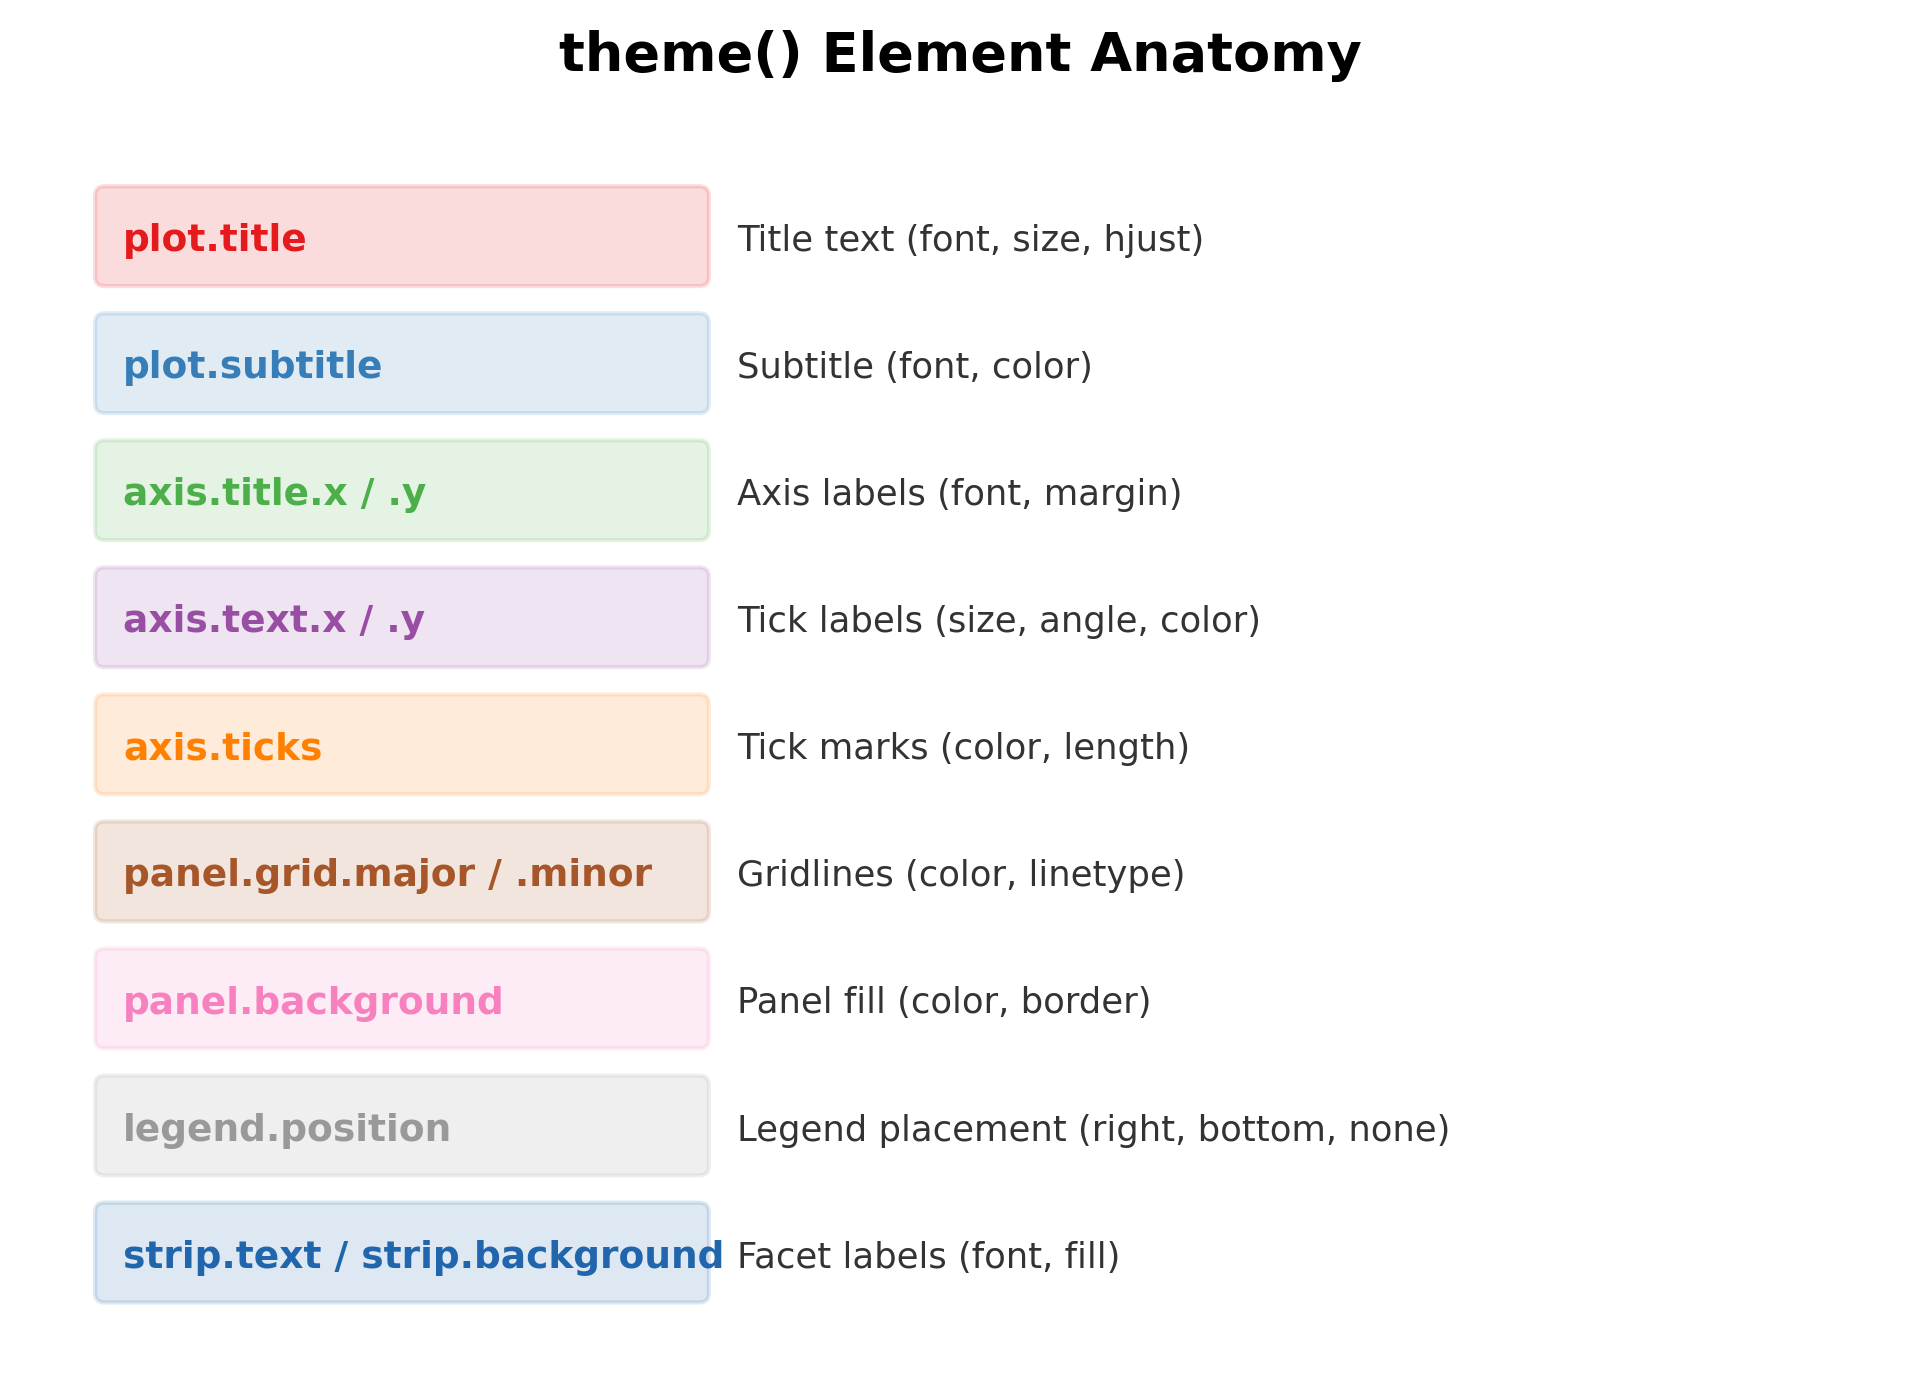
\includegraphics[width=\textwidth]{m1_8_theme_anatomy.png}
\begin{exampleblock}{Data Insight}
    \scriptsize \texttt{theme()} calls are \textbf{additive}: start with a base theme, then override individual elements. Order matters --- later \texttt{theme()} calls override earlier ones.
\end{exampleblock}
\end{column}
\end{columns}
\end{frame}

% ── 218 ──
\begin{frame}[fragile]{Customizing Theme --- \Python}\smark{218/300}
\begin{columns}[T]
\begin{column}{0.48\textwidth}
\begin{lstlisting}[style=Pystyle]
# plotnine
from plotnine import (
    theme, element_text,
    element_blank, element_rect)

(ggplot(...) + theme_minimal()
 + theme(
    plot_title=element_text(
      face="bold", size=14),
    axis_title=element_text(
      size=11, color="#333"),
    panel_grid_minor=
      element_blank(),
    legend_position="bottom",
    strip_text=element_text(
      face="bold")))
\end{lstlisting}
\end{column}
\begin{column}{0.48\textwidth}
\begin{lstlisting}[style=Pystyle]
# matplotlib equivalent
ax.set_title("Title",
    fontweight="bold", fontsize=14)
ax.set_xlabel("X", fontsize=11,
    color="#333")
ax.yaxis.grid(False, which="minor")
ax.legend(loc="lower center",
    bbox_to_anchor=(0.5, -0.2),
    ncol=3)
\end{lstlisting}
\vspace{0.1cm}
\begin{alertblock}{Pro-Tip}
    \scriptsize plotnine uses underscores (\texttt{plot\_title}); ggplot2 uses dots (\texttt{plot.title}). Everything else is identical.
\end{alertblock}
\end{column}
\end{columns}
\end{frame}

% ── 219 ──
\begin{frame}{Gridlines: How Much Is Enough?}
\smark{219/300}
\begin{columns}[T]
\begin{column}{0.50\textwidth}
\begin{itemize}
    \item \textbf{Major gridlines}: help read approximate values
    \item \textbf{Minor gridlines}: usually noise --- remove them
    \item Tufte: remove gridlines entirely when the data is dense enough to anchor perception
    \item Compromise: light major grid ($\alpha=0.15$), no minor
\end{itemize}
\end{column}
\begin{column}{0.47\textwidth}
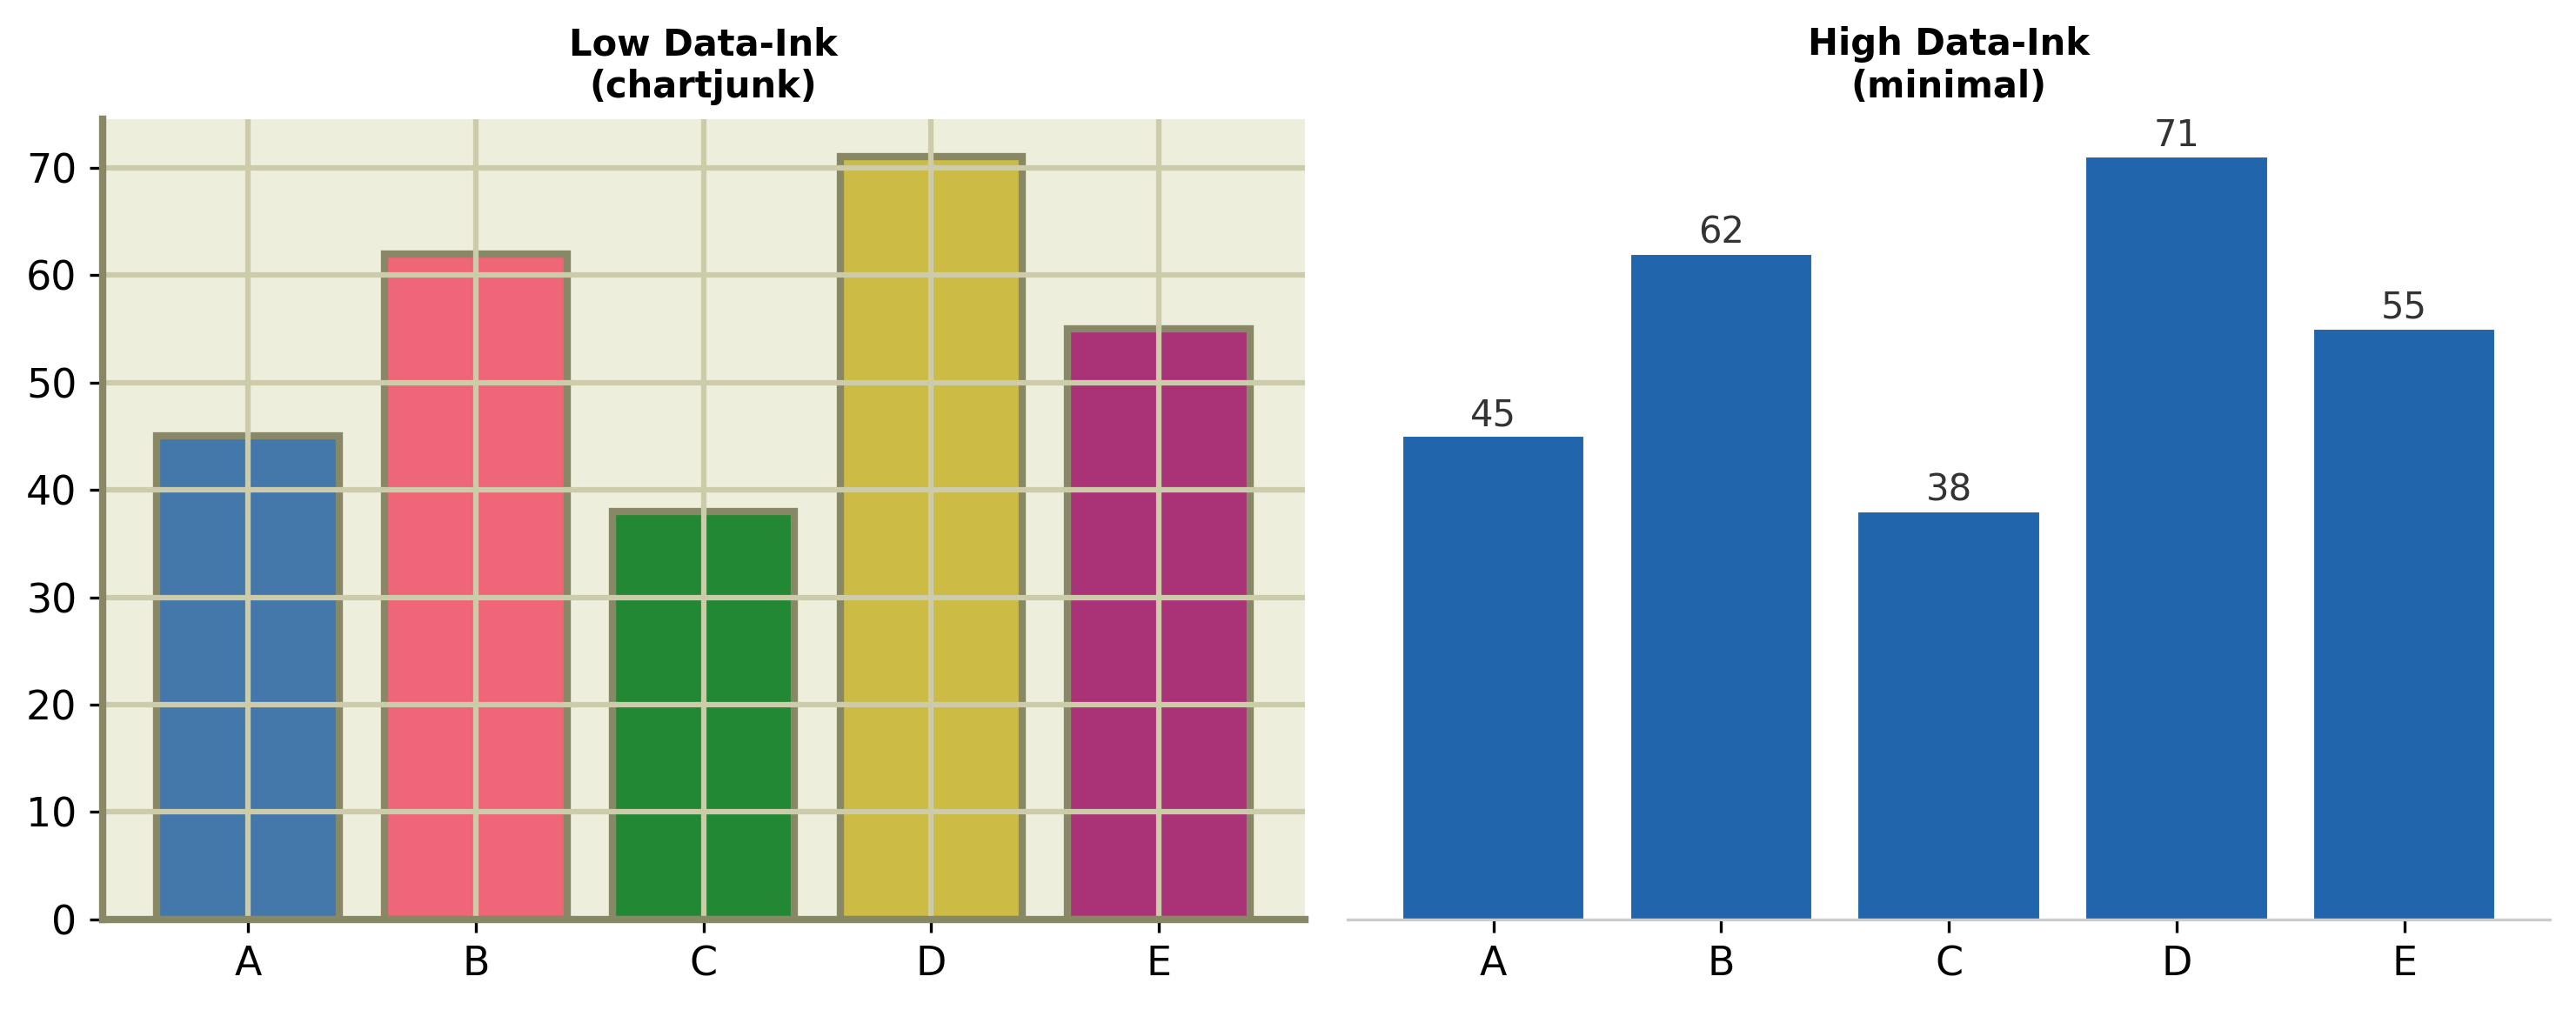
\includegraphics[width=\textwidth]{m1_8_data_ink.png}
\begin{exampleblock}{Data Insight}
    \scriptsize Left: heavy grid competes with data for attention. Right: direct labels replace gridlines entirely --- the numbers are \emph{on} the bars. Maximum data-ink ratio.
\end{exampleblock}
\end{column}
\end{columns}
\end{frame}

% ── 220 ──
\begin{frame}[fragile]{Gridline Control --- Code}\smark{220/300}
\begin{columns}[T]
\begin{column}{0.48\textwidth}
\begin{lstlisting}[style=Rstyle]
# Remove all gridlines
theme(panel.grid = element_blank())

# Keep major only, light
theme(
  panel.grid.major =
    element_line(color="#EEEEEE"),
  panel.grid.minor =
    element_blank())

# Horizontal only (bar charts)
theme(
  panel.grid.major.x =
    element_blank())
\end{lstlisting}
\end{column}
\begin{column}{0.48\textwidth}
\begin{lstlisting}[style=Pystyle]
# matplotlib
ax.grid(False)          # all off
ax.yaxis.grid(True,     # y major on
    alpha=0.15, color="#EEE")
ax.xaxis.grid(False)    # x off

# plotnine
theme(
  panel_grid_major=
    element_line(color="#EEEEEE"),
  panel_grid_minor=
    element_blank())
\end{lstlisting}
\end{column}
\end{columns}
\end{frame}

% ── 221 ──
\begin{frame}{Legend Positioning}
\smark{221/300}
\centering
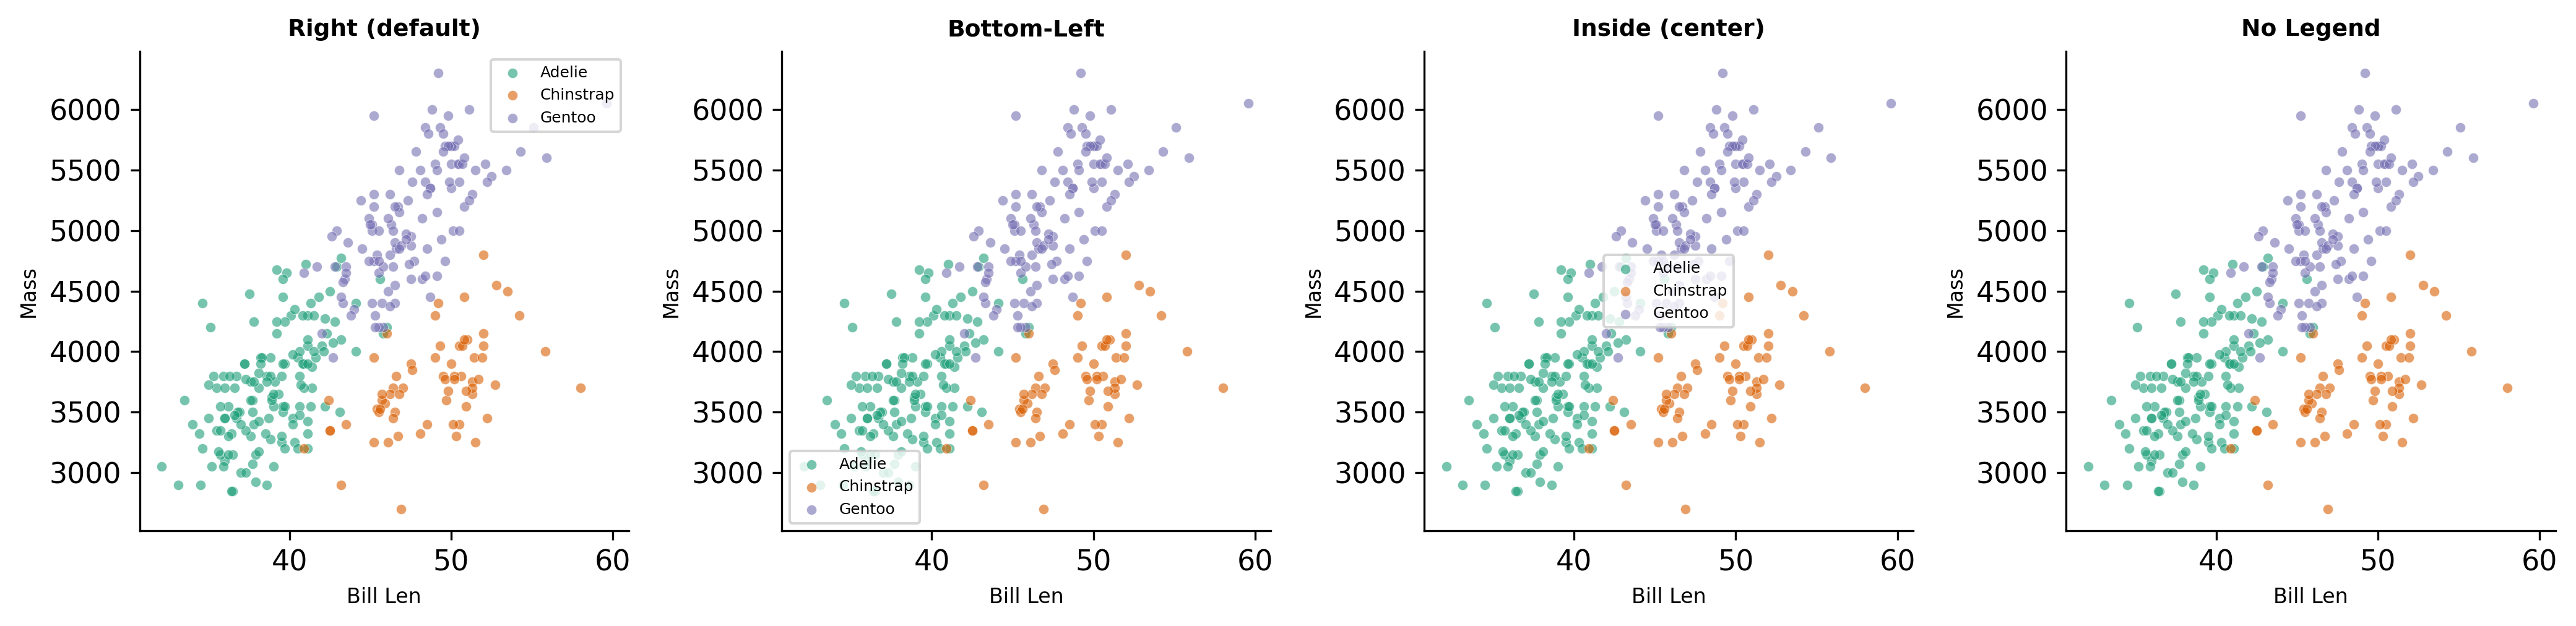
\includegraphics[width=0.92\textwidth]{m1_8_legend_pos.png}

\vspace{0.2cm}
\begin{alertblock}{Pro-Tip}
    \scriptsize Right (default) is fine for exploration. For publication: \textbf{bottom} saves horizontal space; \textbf{inside} the plot area uses dead space; \textbf{none} when facet labels already identify groups.
\end{alertblock}
\end{frame}

% ── 222 ──
\begin{frame}[fragile]{Legend Customization --- Code}\smark{222/300}
\begin{columns}[T]
\begin{column}{0.48\textwidth}
\begin{lstlisting}[style=Rstyle]
theme(
  # Position: string or c(x,y)
  legend.position = "bottom",
  # or inside plot:
  legend.position = c(0.85, 0.2),
  # Title
  legend.title = element_text(
    face="bold", size=10),
  # Remove legend entirely
  legend.position = "none",
  # Horizontal layout
  legend.direction =
    "horizontal"
)
\end{lstlisting}
\end{column}
\begin{column}{0.48\textwidth}
\begin{lstlisting}[style=Pystyle]
# plotnine
theme(legend_position="bottom")
theme(legend_position=(0.85,0.2))
theme(legend_position="none")

# matplotlib
ax.legend(
    loc="lower right",
    fontsize=8,
    framealpha=0.8,
    ncol=3,
    title="Species",
    title_fontsize=9)
# Remove
ax.get_legend().remove()
\end{lstlisting}
\end{column}
\end{columns}
\end{frame}

% ── 223 ──
\begin{frame}{Font Selection for Data Graphics}
\smark{223/300}
\centering
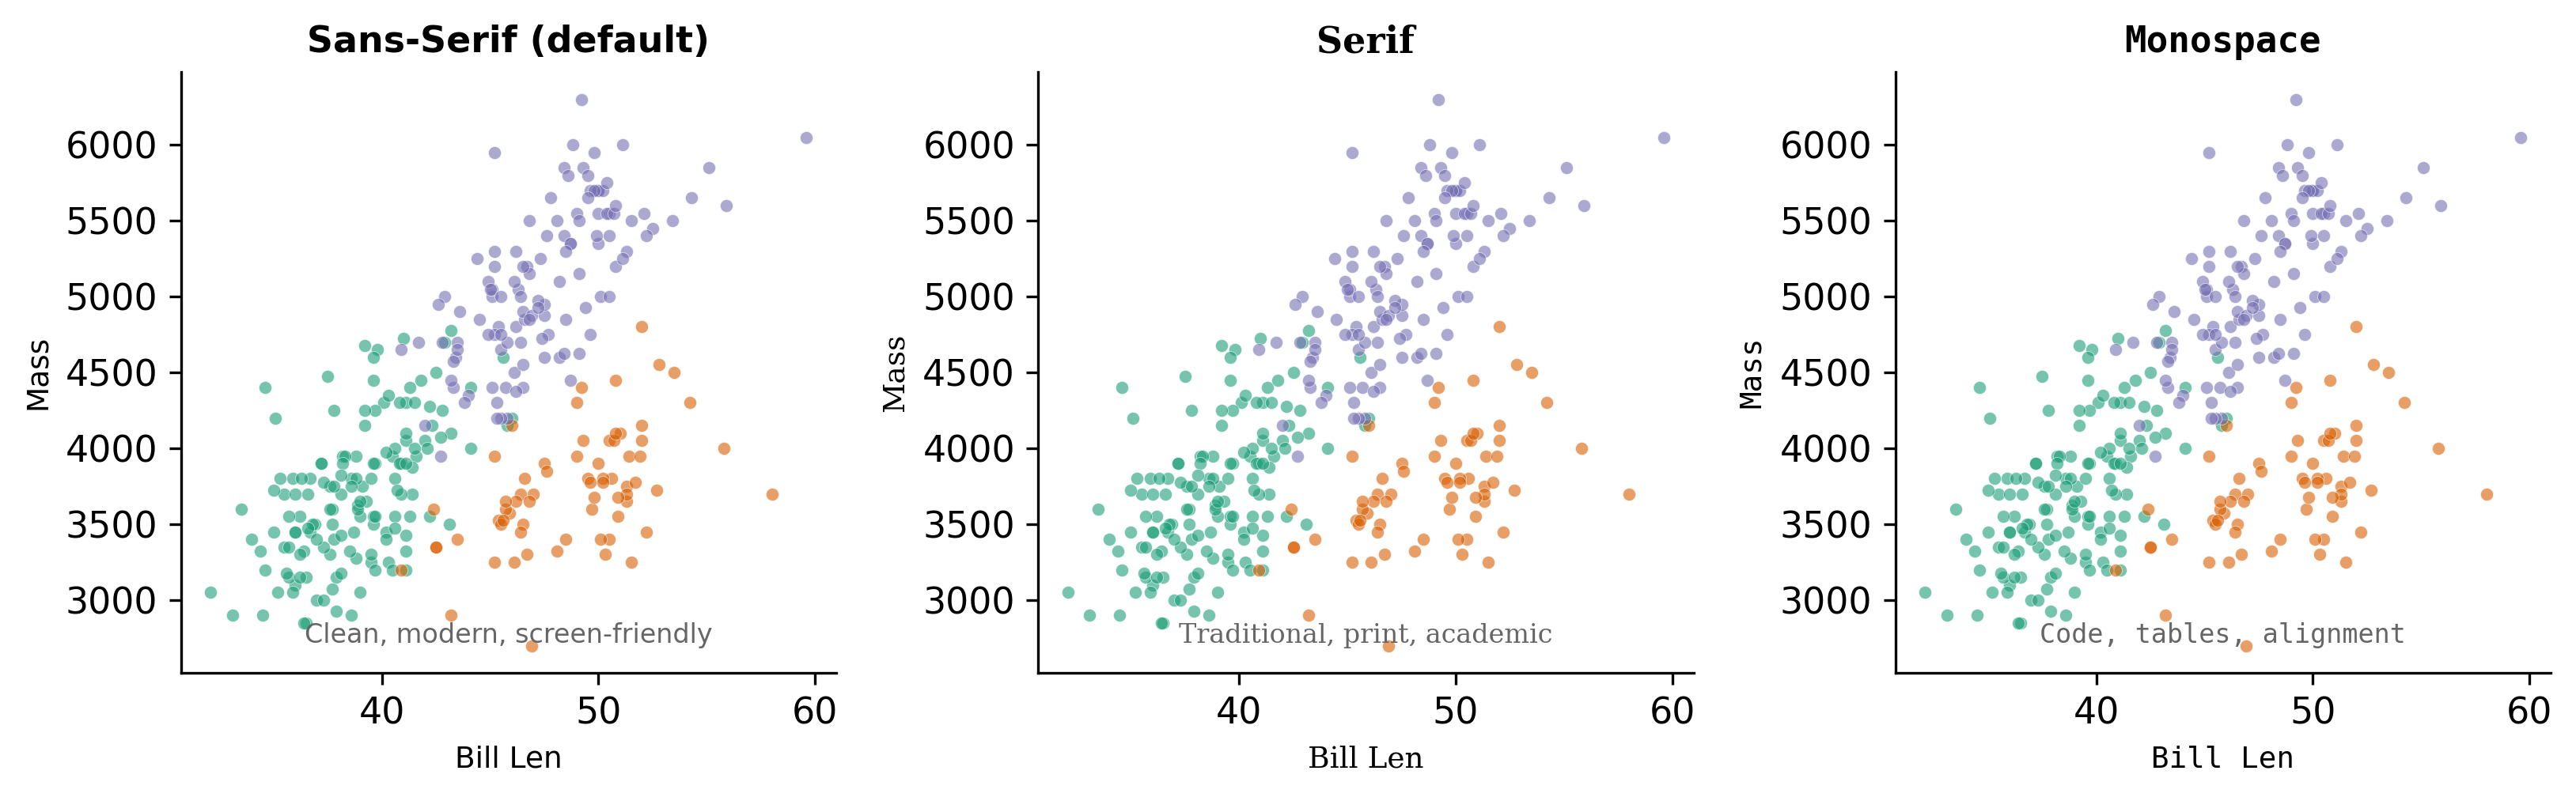
\includegraphics[width=0.88\textwidth]{m1_8_fonts.png}

\vspace{0.2cm}
\begin{columns}[T]
\begin{column}{0.48\textwidth}
\begin{itemize}
    \item \textbf{Sans-serif} (Fira Sans, Helvetica, Arial): clean, modern, screen-friendly --- default for most dataviz
    \item \textbf{Serif} (Times, Palatino): academic, print
    \item \textbf{Monospace} (Fira Mono, Courier): code snippets, alignment
\end{itemize}
\end{column}
\begin{column}{0.48\textwidth}
\begin{alertblock}{Pro-Tip}
    \scriptsize Use \textbf{one font family} throughout. Sans-serif body + monospace for code annotations is the safe combo. Avoid decorative/display fonts in charts.
\end{alertblock}
\end{column}
\end{columns}
\end{frame}

% ── 224 ──
\begin{frame}[fragile]{Custom Fonts --- Code}\smark{224/300}
\begin{columns}[T]
\begin{column}{0.48\textwidth}
\begin{lstlisting}[style=Rstyle]
# showtext for Google Fonts
library(showtext)
font_add_google("Fira Sans",
                "firasans")
showtext_auto()

theme(
  text = element_text(
    family = "firasans"),
  plot.title = element_text(
    family = "firasans",
    face = "bold")
)
\end{lstlisting}
\end{column}
\begin{column}{0.48\textwidth}
\begin{lstlisting}[style=Pystyle]
# matplotlib font setup
plt.rcParams.update({
    "font.family": "sans-serif",
    "font.sans-serif":
        ["Fira Sans", "Arial"],
    "font.size": 11
})

# Per-element override
ax.set_title("Title",
    fontfamily="serif",
    fontsize=14)
\end{lstlisting}
\vspace{0.1cm}
\begin{exampleblock}{Data Insight}
    \scriptsize R's \texttt{showtext} and Python's \texttt{rcParams} both allow Google Fonts. Ensure the font is installed on the system or use \texttt{font\_add\_google()} / \texttt{matplotlib.font\_manager}.
\end{exampleblock}
\end{column}
\end{columns}
\end{frame}

% ── 225 ──
\begin{frame}{Dark Themes for Presentations}
\smark{225/300}
\begin{columns}[T]
\begin{column}{0.50\textwidth}
\begin{itemize}
    \item Dark background + light data = high contrast on projectors
    \item Reduce eye strain in dim rooms
    \item Requires \textbf{brighter} color palettes (pastels, not saturated darks)
    \item \textbf{Never} use for print --- ink-heavy and unreadable
\end{itemize}
\end{column}
\begin{column}{0.47\textwidth}
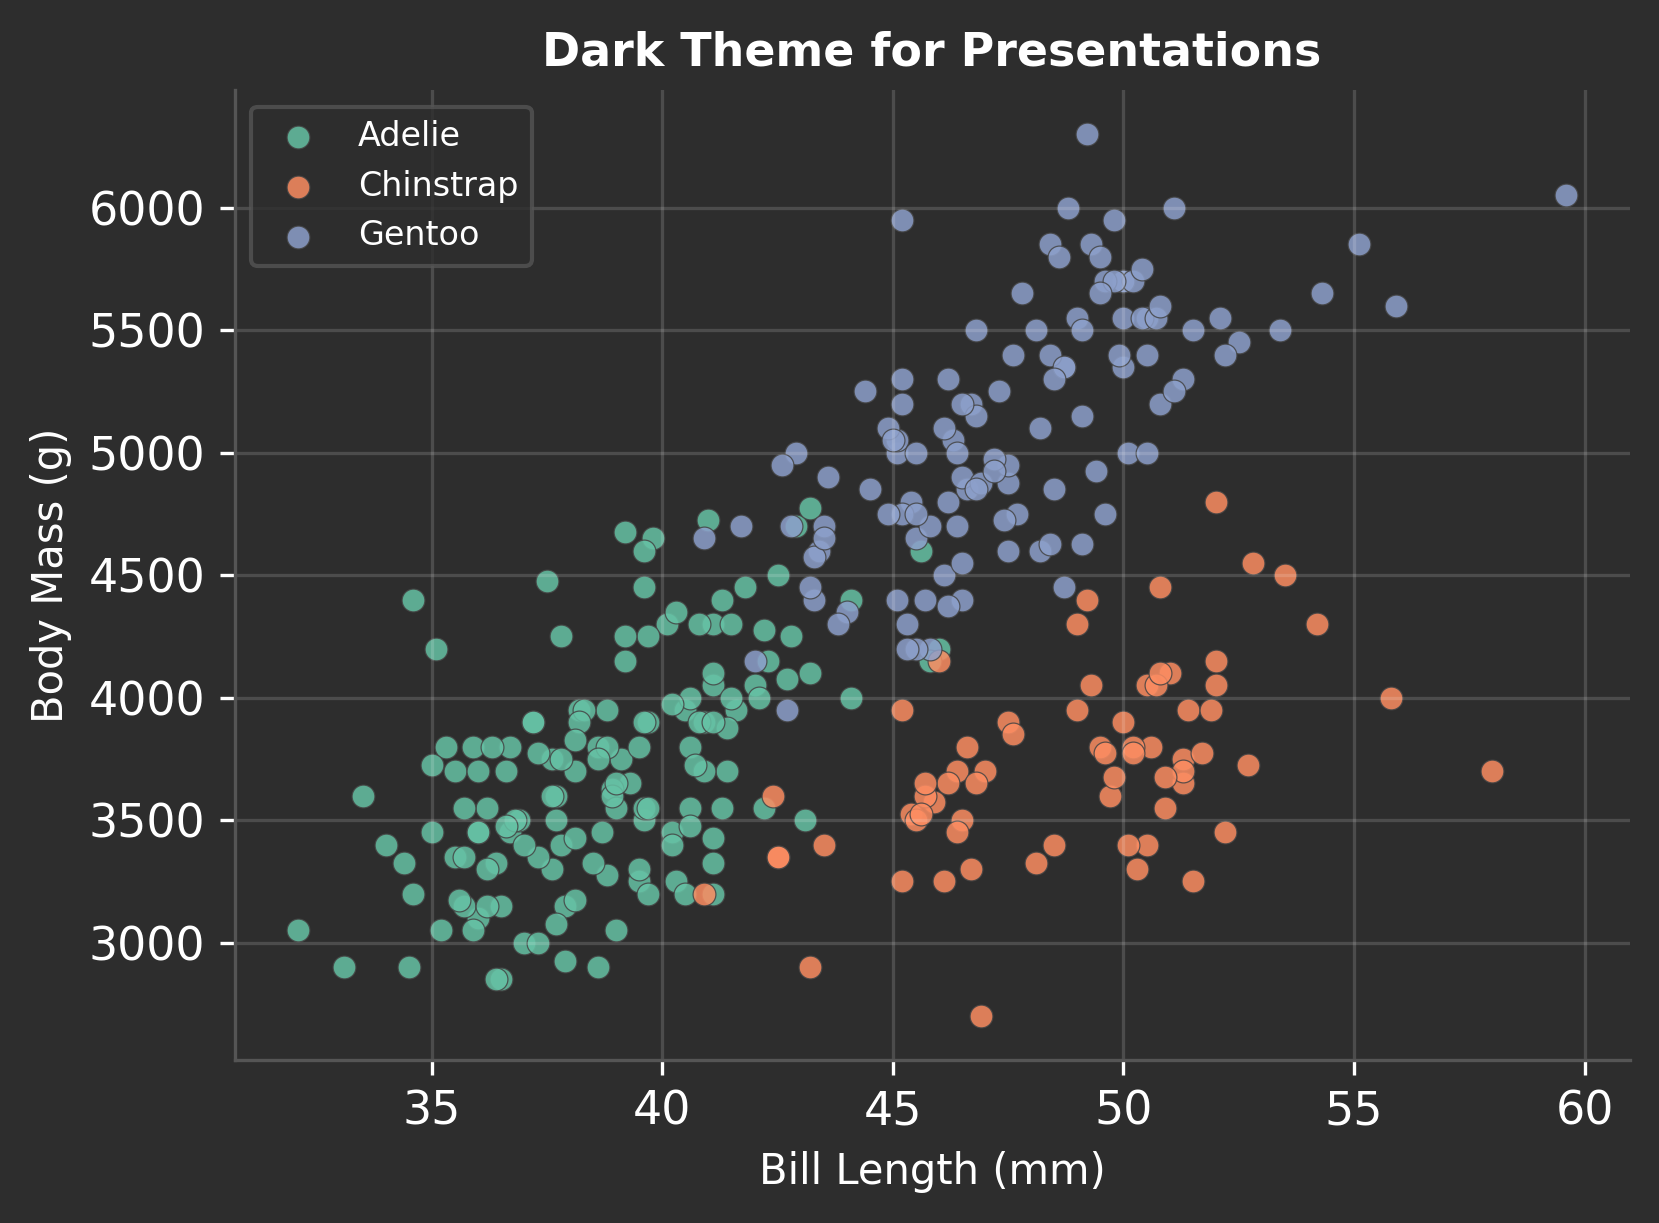
\includegraphics[width=\textwidth]{m1_8_dark_theme.png}
\begin{alertblock}{Pro-Tip}
    \scriptsize In ggplot2: \texttt{theme\_dark()} + custom lighter palette. In matplotlib: \texttt{plt.style.use("dark\_background")}. In seaborn: \texttt{sns.set\_style("darkgrid")}.
\end{alertblock}
\end{column}
\end{columns}
\end{frame}

% ── 226 ──
\begin{frame}[fragile]{Dark Theme --- Code}\smark{226/300}
\begin{columns}[T]
\begin{column}{0.48\textwidth}
\begin{lstlisting}[style=Rstyle]
ggplot(penguins, aes(
    bill_length_mm, body_mass_g,
    color = species)) +
  geom_point(alpha=0.8, size=2)+
  scale_color_manual(values =
    c("#66C2A5","#FC8D62",
      "#8DA0CB")) +
  theme_dark(base_size = 14) +
  theme(
    plot.background =
      element_rect(fill="#2D2D2D"),
    panel.background =
      element_rect(fill="#2D2D2D"),
    legend.background =
      element_rect(fill="#2D2D2D"),
    text = element_text(
      color="white"))
\end{lstlisting}
\end{column}
\begin{column}{0.48\textwidth}
\begin{lstlisting}[style=Pystyle]
# matplotlib one-liner
plt.style.use("dark_background")

# Then plot normally:
for sp, c in zip(species,
    ["#66C2A5","#FC8D62","#8DA0CB"]):
    sub = pen[pen["species"]==sp]
    ax.scatter(sub.x, sub.y,
               c=c, label=sp)

# Revert afterward
plt.style.use("default")
\end{lstlisting}
\vspace{0.1cm}
\begin{exampleblock}{Data Insight}
    \scriptsize \texttt{plt.style.use()} is global. Use \texttt{with plt.style.context("dark\_background"):} for a temporary dark block.
\end{exampleblock}
\end{column}
\end{columns}
\end{frame}

% ── 227 ──
\begin{frame}{Building a Custom Brand Theme}
\smark{227/300}
\begin{columns}[T]
\begin{column}{0.50\textwidth}
\begin{itemize}
    \item Pick \textbf{3 colors}: primary, secondary, accent
    \item Choose \textbf{1 font family} (with bold/italic variants)
    \item Define background: white, off-white, or brand tint
    \item Set gridline style: light, dashed, or none
    \item Wrap in a \textbf{function} for reuse across projects
\end{itemize}
\end{column}
\begin{column}{0.47\textwidth}
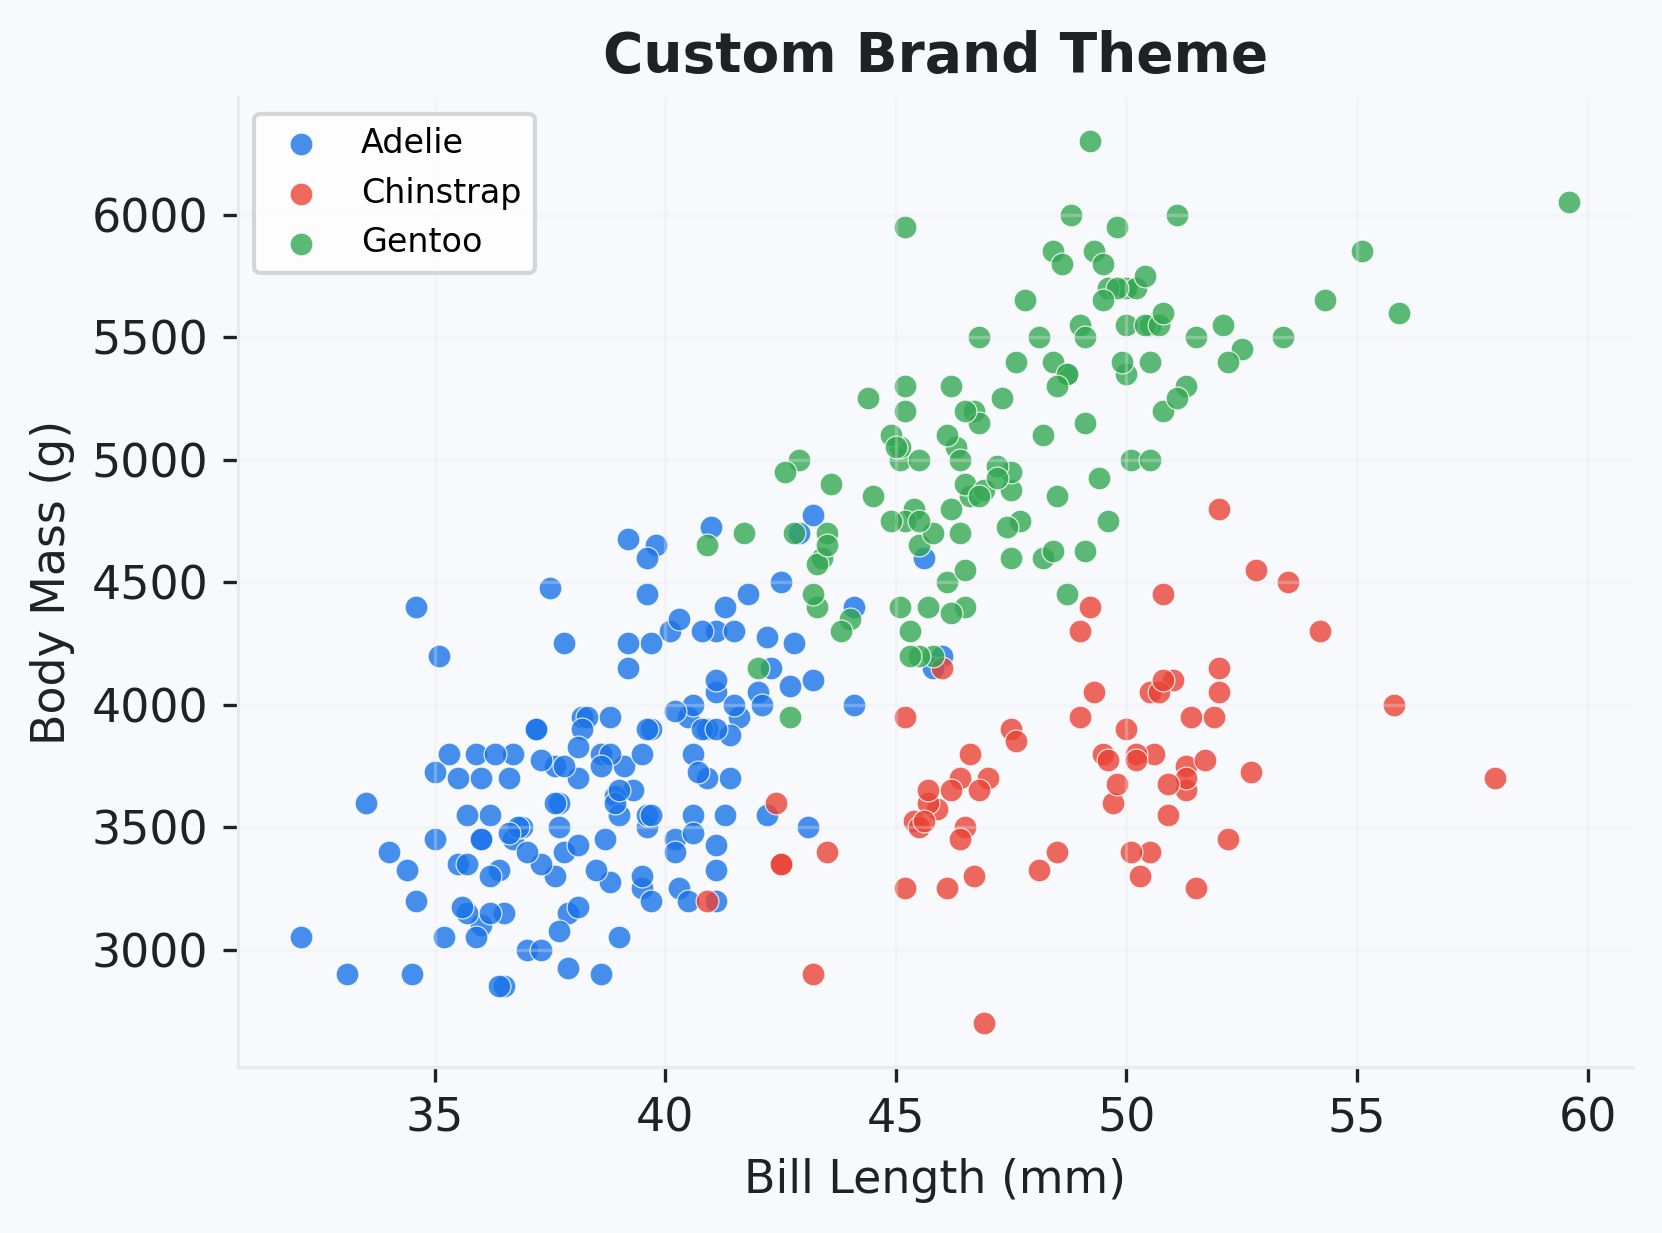
\includegraphics[width=\textwidth]{m1_8_brand_theme.png}
\begin{exampleblock}{Data Insight}
    \scriptsize This example uses Google's blue (\texttt{\#1A73E8}), red, and green on an off-white background (\texttt{\#F7F9FC}) with light gray gridlines. Consistent across all figures.
\end{exampleblock}
\end{column}
\end{columns}
\end{frame}

% ── 228 ──
\begin{frame}[fragile]{Custom Theme Function --- \Rlang}\smark{228/300}
\begin{columns}[T]
\begin{column}{0.55\textwidth}
\begin{lstlisting}[style=Rstyle]
theme_brand <- function(
    base_size = 12) {
  theme_minimal(
    base_size = base_size) +
  theme(
    text = element_text(
      family = "Fira Sans",
      color = "#202124"),
    plot.title = element_text(
      face = "bold", size = 14),
    panel.background =
      element_rect(
        fill = "#F7F9FC",
        color = NA),
    panel.grid.major =
      element_line(
        color = "#E8EAED"),
    panel.grid.minor =
      element_blank(),
    legend.position = "bottom"
  )
}
# Usage: ggplot(...) + theme_brand()
\end{lstlisting}
\end{column}
\begin{column}{0.42\textwidth}
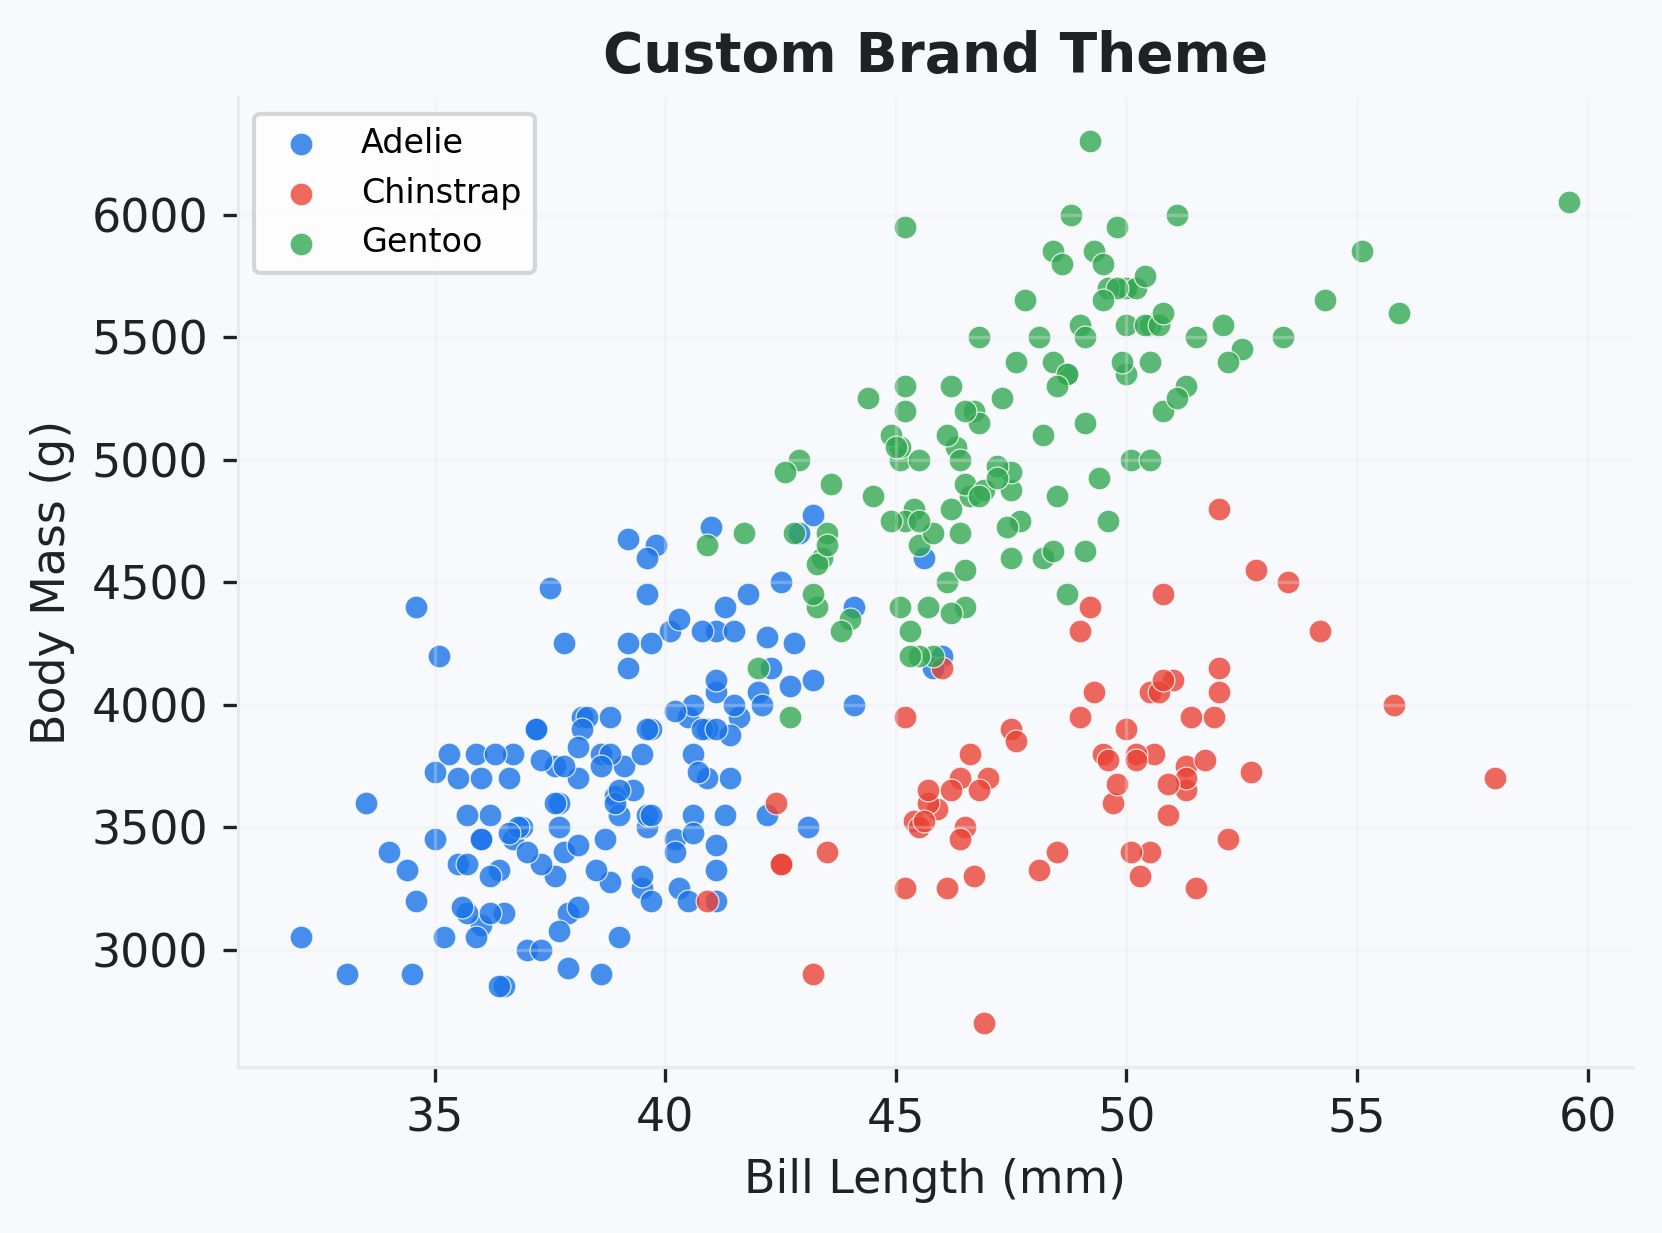
\includegraphics[width=\textwidth]{m1_8_brand_theme.png}
\begin{alertblock}{Pro-Tip}
    \scriptsize Save your custom theme in a separate \texttt{theme\_brand.R} file. Source it at the top of every script: \texttt{source("theme\_brand.R")}.
\end{alertblock}
\end{column}
\end{columns}
\end{frame}

% ── 229 ──
\begin{frame}[fragile]{Custom Theme Function --- \Python}\smark{229/300}
\begin{columns}[T]
\begin{column}{0.55\textwidth}
\begin{lstlisting}[style=Pystyle]
# plotnine custom theme
from plotnine import (theme,
    element_text, element_rect,
    element_line, element_blank)

def theme_brand(base_size=12):
    return (
        theme_minimal(base_size) +
        theme(
          plot_title=element_text(
            face="bold", size=14),
          panel_background=
            element_rect(
              fill="#F7F9FC"),
          panel_grid_major=
            element_line(
              color="#E8EAED"),
          panel_grid_minor=
            element_blank(),
          legend_position="bottom"))
# Usage: ggplot(...) + theme_brand()
\end{lstlisting}
\end{column}
\begin{column}{0.42\textwidth}
\begin{lstlisting}[style=Pystyle]
# matplotlib equivalent
def apply_brand(fig, ax):
    fig.patch.set_facecolor(
        "#F7F9FC")
    ax.set_facecolor("#F7F9FC")
    ax.grid(True, alpha=0.3,
            color="#E8EAED")
    for s in ax.spines.values():
        s.set_color("#E8EAED")
\end{lstlisting}
\vspace{0.1cm}
\begin{exampleblock}{Data Insight}
    \scriptsize plotnine themes compose with \texttt{+}. matplotlib requires a helper function that mutates the axes object.
\end{exampleblock}
\end{column}
\end{columns}
\end{frame}

% ── 230 ──
\begin{frame}{Extension Theme Packages}
\smark{230/300}
\centering\small
\begin{tabular}{@{}lll@{}}
    \toprule
    \textbf{Package} & \textbf{Language} & \textbf{Themes Included} \\
    \midrule
    \texttt{ggthemes}    & R      & Economist, FiveThirtyEight, Tufte, WSJ \\
    \texttt{hrbrthemes}  & R      & Modern, typography-focused \\
    \texttt{tvthemes}    & R      & TV show themes (fun, not for publication) \\
    \texttt{ggthemr}     & R      & Pre-built palettes + themes \\
    \texttt{SciencePlots} & Python & Nature, Science, IEEE journal styles \\
    \texttt{mplcyberpunk} & Python & Neon/glow themes \\
    \bottomrule
\end{tabular}

\vspace{0.3cm}
\begin{exampleblock}{Data Insight}
    \scriptsize \texttt{ggthemes::theme\_fivethirtyeight()} and \texttt{SciencePlots} with \texttt{plt.style.use("science")} are the most practical for real work. TV themes are for Twitter, not for Nature.
\end{exampleblock}
\end{frame}

% ── 231 ──
\begin{frame}[fragile]{Extension Themes --- Code}\smark{231/300}
\begin{columns}[T]
\begin{column}{0.48\textwidth}
\begin{lstlisting}[style=Rstyle]
library(ggthemes)

# FiveThirtyEight
ggplot(...) +
  theme_fivethirtyeight()

# The Economist
ggplot(...) +
  theme_economist() +
  scale_color_economist()

# Tufte (minimal ink)
ggplot(...) +
  theme_tufte()

library(hrbrthemes)
ggplot(...) +
  theme_ipsum()
\end{lstlisting}
\end{column}
\begin{column}{0.48\textwidth}
\begin{lstlisting}[style=Pystyle]
# pip install SciencePlots
import scienceplots
plt.style.use("science")

# Multiple styles compose:
plt.style.use(
    ["science","no-latex"])

# IEEE format
plt.style.use(
    ["science","ieee"])

# Nature format
plt.style.use(
    ["science","nature"])
\end{lstlisting}
\vspace{0.1cm}
\begin{alertblock}{Pro-Tip}
    \scriptsize \texttt{SciencePlots} styles auto-set figure size, font, and DPI to journal requirements. One line replaces 20 \texttt{rcParams} tweaks.
\end{alertblock}
\end{column}
\end{columns}
\end{frame}

% ── 232 ──
\begin{frame}{\texttt{theme\_set()}: Global Defaults}
\smark{232/300}
\begin{columns}[T]
\begin{column}{0.50\textwidth}
\begin{itemize}
    \item \texttt{theme\_set()} applies a theme to \textbf{all subsequent} plots in a session/script
    \item Eliminates repetitive \texttt{+ theme\_minimal()} on every plot
    \item Override per-plot by adding \texttt{+ theme()} after
    \item Reset with \texttt{theme\_set(theme\_gray())}
\end{itemize}
\end{column}
\begin{column}{0.47\textwidth}
\begin{alertblock}{Pro-Tip}
    \scriptsize Put \texttt{theme\_set(theme\_brand())} at the top of your analysis script, right after loading libraries. Every figure will be on-brand by default.
\end{alertblock}
\vspace{0.2cm}
\begin{exampleblock}{Data Insight}
    \scriptsize In matplotlib: \texttt{plt.rcParams.update(\{...\})} is the equivalent of \texttt{theme\_set()}. In seaborn: \texttt{sns.set\_theme()} at the top.
\end{exampleblock}
\end{column}
\end{columns}
\end{frame}

% ── 233 ──
\begin{frame}[fragile]{\texttt{theme\_set} --- Code}\smark{233/300}
\begin{columns}[T]
\begin{column}{0.48\textwidth}
\begin{lstlisting}[style=Rstyle]
# Set once at top of script
theme_set(
  theme_minimal(base_size=12) +
  theme(
    plot.title = element_text(
      face = "bold"),
    panel.grid.minor =
      element_blank()))

# All subsequent plots inherit:
ggplot(df1, ...) + geom_point()
ggplot(df2, ...) + geom_line()
# Both get the custom theme
\end{lstlisting}
\end{column}
\begin{column}{0.48\textwidth}
\begin{lstlisting}[style=Pystyle]
# matplotlib global
plt.rcParams.update({
    "font.size": 12,
    "axes.titleweight": "bold",
    "axes.grid": True,
    "grid.alpha": 0.15,
    "axes.spines.top": False,
    "axes.spines.right": False})

# seaborn global
sns.set_theme(
    style="whitegrid",
    context="paper",
    font_scale=1.1)
\end{lstlisting}
\end{column}
\end{columns}
\end{frame}

% ── 234 ──
\begin{frame}{The Before/After Makeover}
\smark{234/300}
\centering
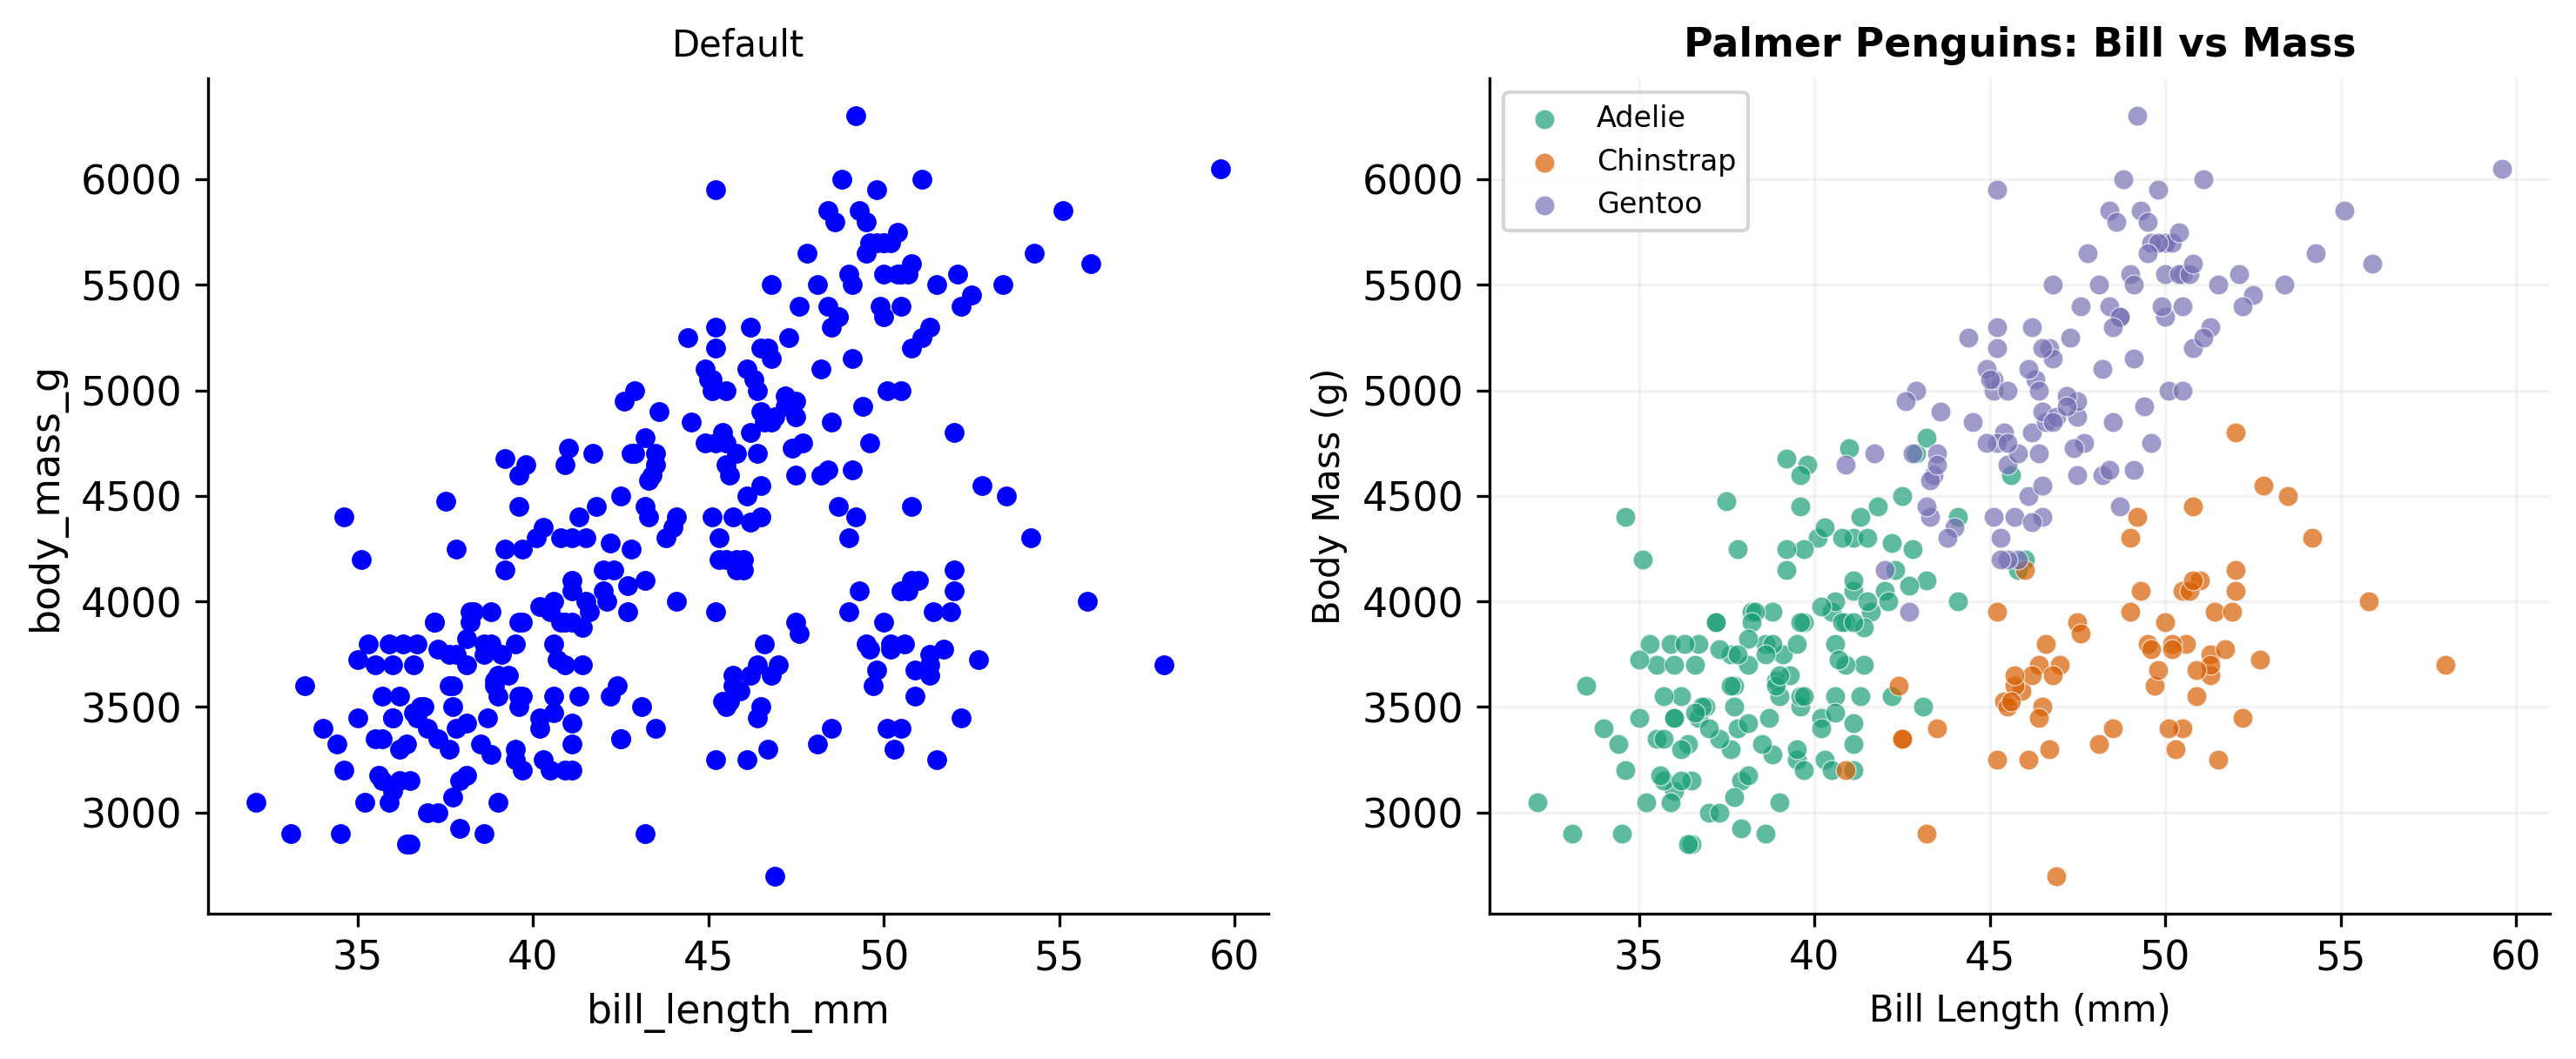
\includegraphics[width=0.88\textwidth]{m1_8_before_after.png}

\vspace{0.2cm}
\begin{exampleblock}{Data Insight}
    \scriptsize Left: default everything --- generic blue, no color grouping, raw variable names as labels, cluttered. Right: species colored, clean labels, bold title, light grid, legend positioned. Same data, same geom --- only theme and aesthetic mapping changed.
\end{exampleblock}
\end{frame}

% ── 235 ──
\begin{frame}{Makeover Checklist}
\smark{235/300}
\begin{columns}[T]
\begin{column}{0.48\textwidth}
\textbf{Labels:}
\begin{itemize}
    \item Title: analytical claim, not description
    \item Axis labels: human-readable, with units
    \item No variable names (\texttt{bill\_length\_mm} $\to$ ``Bill Length (mm)'')
\end{itemize}
\vspace{0.2cm}
\textbf{Colors:}
\begin{itemize}
    \item Map to a meaningful grouping
    \item Use a named palette (not defaults)
    \item Ensure colorblind safety
\end{itemize}
\end{column}
\begin{column}{0.48\textwidth}
\textbf{Grid \& Background:}
\begin{itemize}
    \item Remove minor gridlines
    \item Lighten major gridlines
    \item White or off-white background
\end{itemize}
\vspace{0.2cm}
\textbf{Legend:}
\begin{itemize}
    \item Position where it doesn't occlude data
    \item Remove if facet labels suffice
    \item Direct-label when practical
\end{itemize}
\end{column}
\end{columns}
\end{frame}

% ── 236 ──
\begin{frame}[fragile]{Makeover in One Block --- \Rlang}\smark{236/300}
\begin{columns}[T]
\begin{column}{0.55\textwidth}
\begin{lstlisting}[style=Rstyle]
ggplot(penguins,
  aes(bill_length_mm,
      body_mass_g,
      color = species)) +
  geom_point(alpha=0.7, size=2) +
  scale_color_manual(
    values=c("#1B9E77","#D95F02",
             "#7570B3")) +
  labs(
    title="Heavier penguins have
           longer bills",
    x="Bill Length (mm)",
    y="Body Mass (g)",
    color="Species") +
  theme_minimal(base_size=12) +
  theme(
    plot.title = element_text(
      face="bold"),
    panel.grid.minor =
      element_blank(),
    legend.position = "bottom")
\end{lstlisting}
\end{column}
\begin{column}{0.42\textwidth}
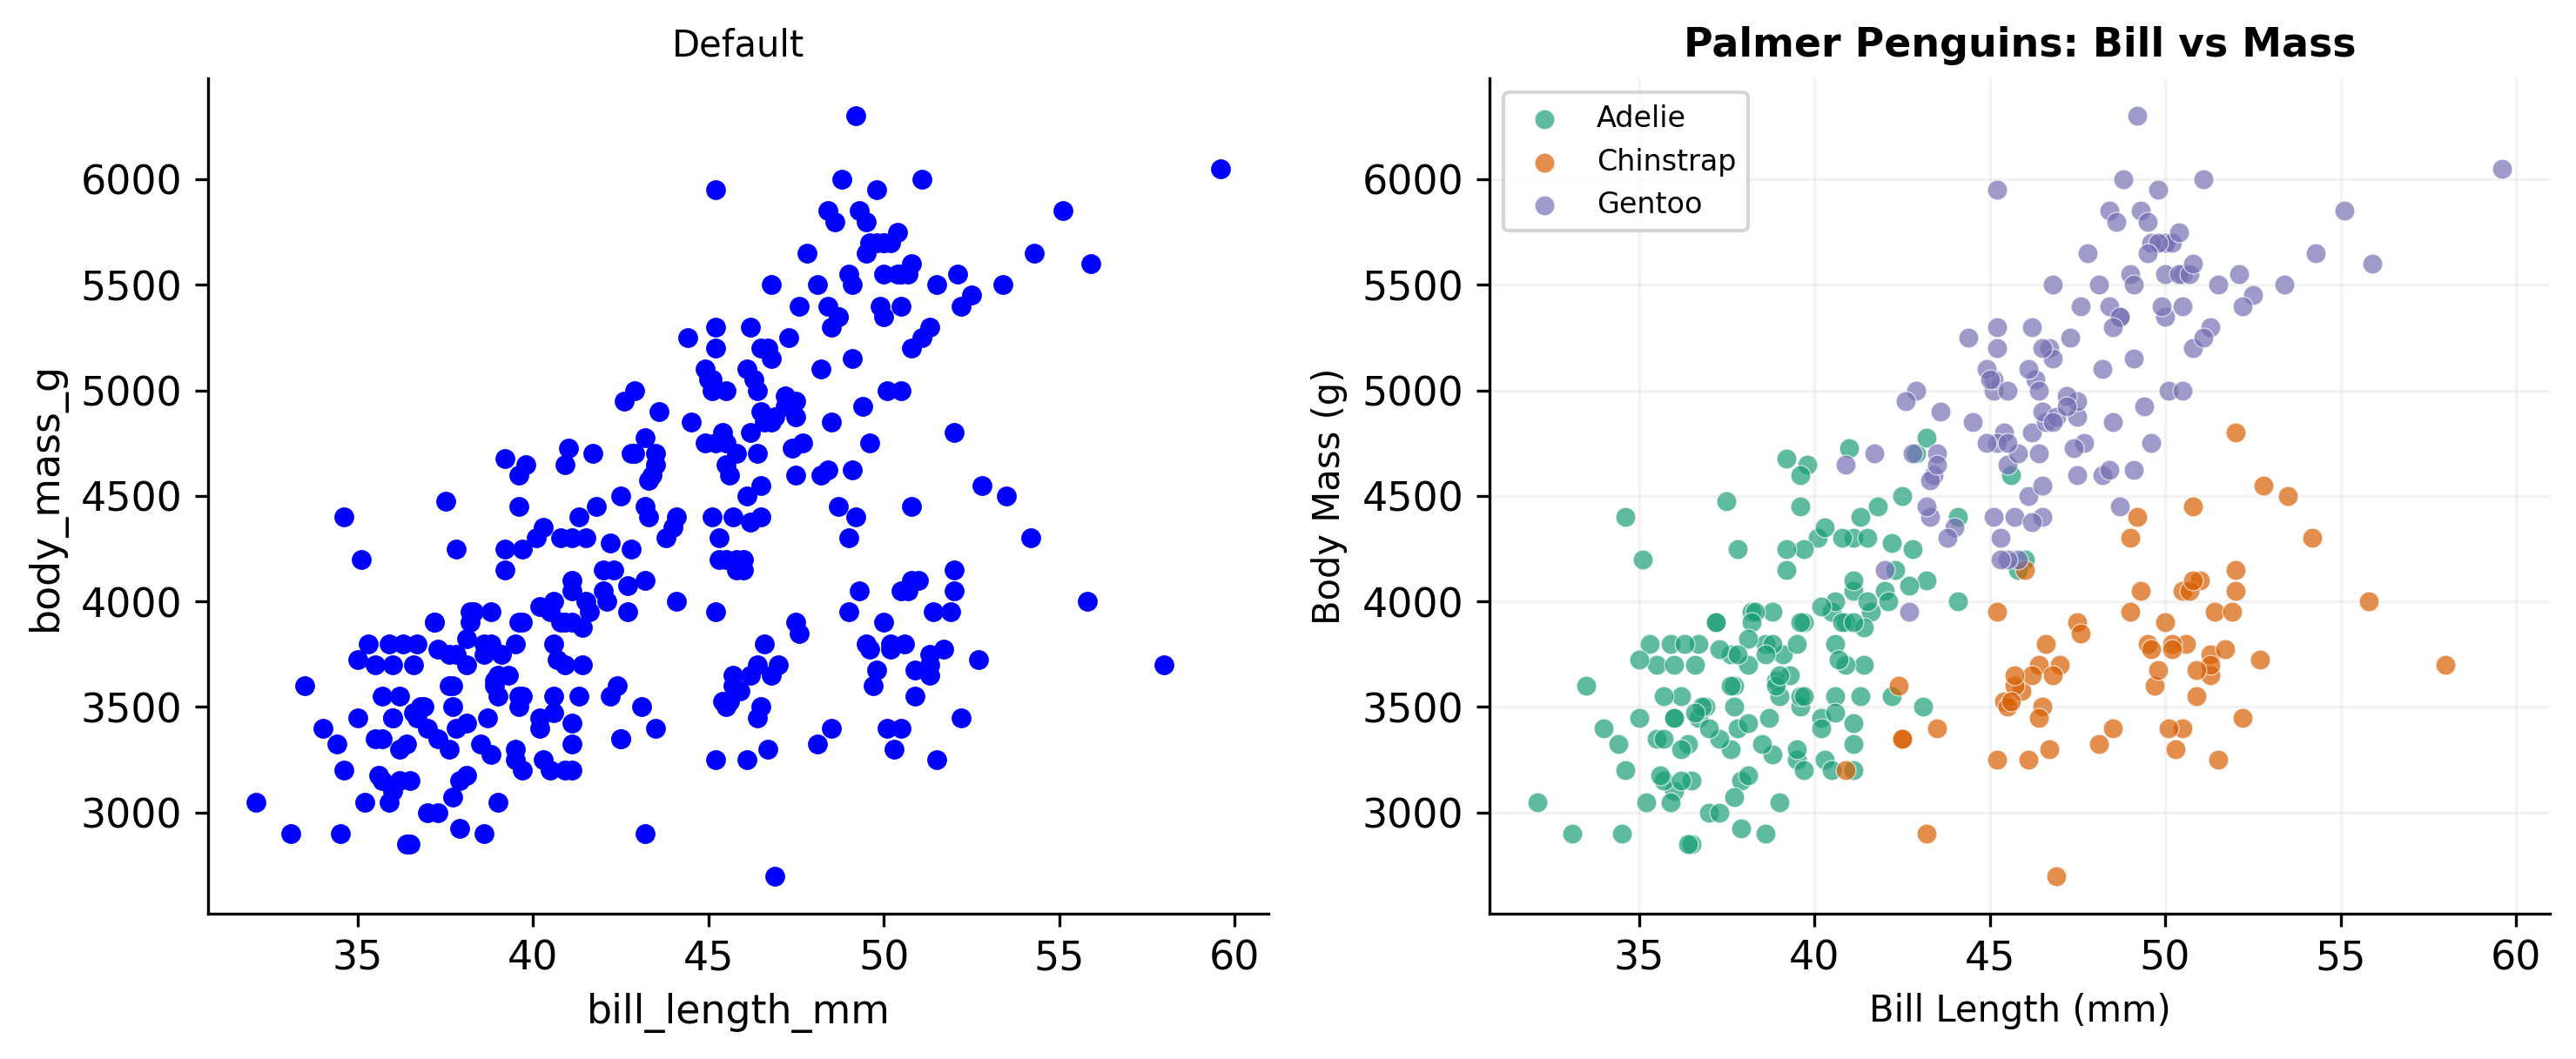
\includegraphics[width=\textwidth]{m1_8_before_after.png}
\begin{alertblock}{Pro-Tip}
    \scriptsize The title should state the \textbf{insight}, not the method: ``Heavier penguins have longer bills'' not ``Scatter plot of bill length vs body mass.''
\end{alertblock}
\end{column}
\end{columns}
\end{frame}

% ── 237 ──
\begin{frame}[fragile]{Makeover in One Block --- \Python}\smark{237/300}
\begin{columns}[T]
\begin{column}{0.55\textwidth}
\begin{lstlisting}[style=Pystyle]
(ggplot(penguins,
   aes("bill_length_mm",
       "body_mass_g",
       color="species"))
 + geom_point(alpha=0.7, size=2)
 + scale_color_manual(
     values=["#1B9E77","#D95F02",
             "#7570B3"])
 + labs(
     title="Heavier penguins have "
           "longer bills",
     x="Bill Length (mm)",
     y="Body Mass (g)",
     color="Species")
 + theme_minimal()
 + theme(
     plot_title=element_text(
       face="bold"),
     panel_grid_minor=
       element_blank(),
     legend_position="bottom"))
\end{lstlisting}
\end{column}
\begin{column}{0.42\textwidth}
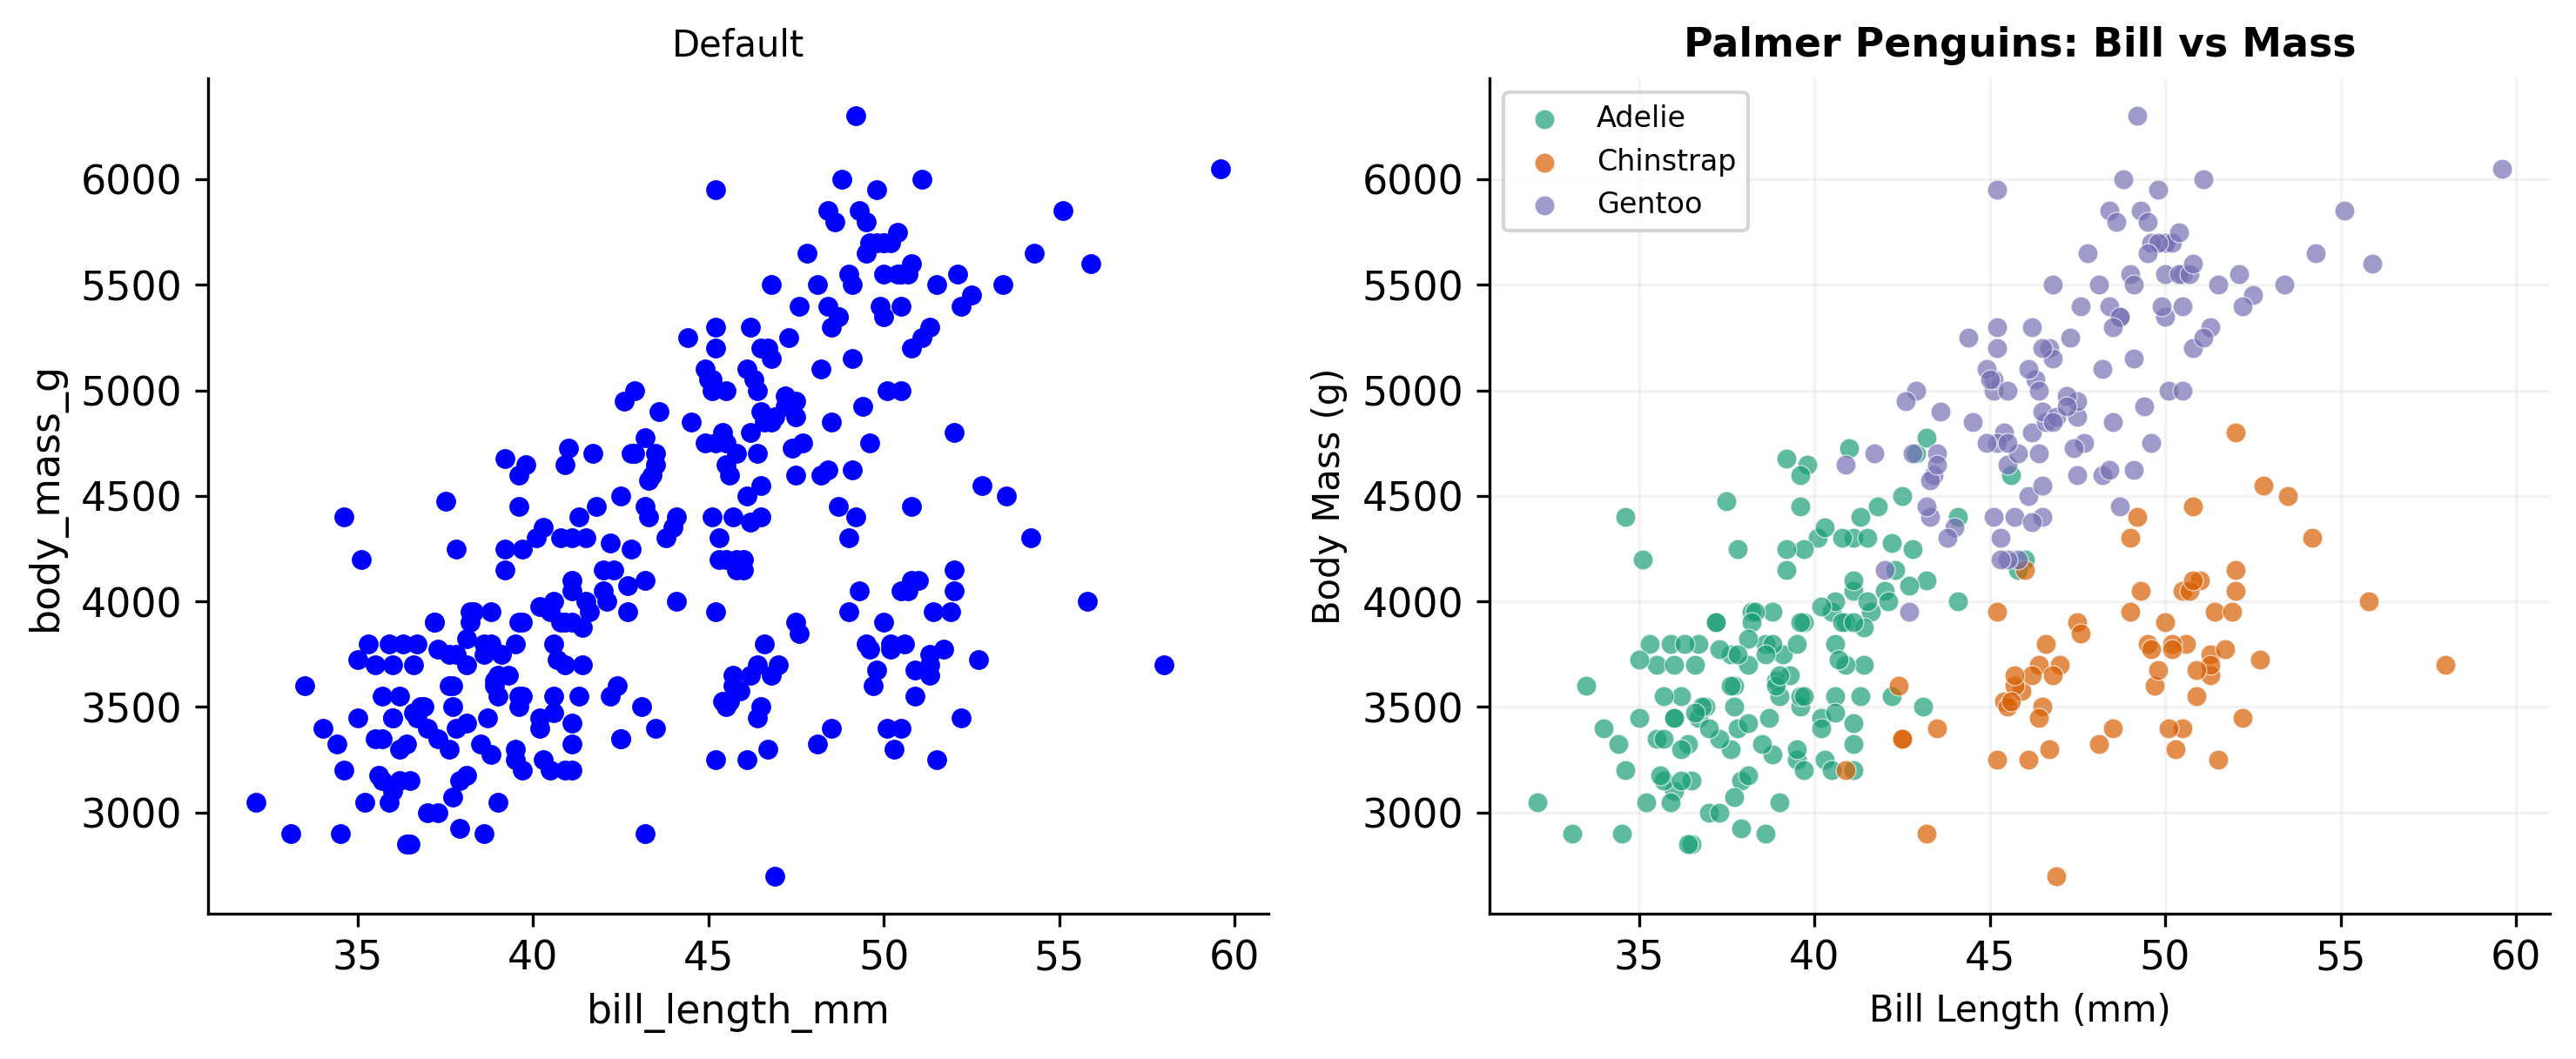
\includegraphics[width=\textwidth]{m1_8_before_after.png}
\end{column}
\end{columns}
\end{frame}

% ── 238 ──
\begin{frame}{Saving Themed Plots Consistently}
\smark{238/300}
\begin{columns}[T]
\begin{column}{0.50\textwidth}
\begin{itemize}
    \item \texttt{ggsave()} respects the theme applied to the plot object
    \item Set \textbf{width, height, dpi} explicitly for reproducibility
    \item Use \textbf{vector} output (PDF, SVG) for publication; \textbf{raster} (PNG) for slides
    \item Module 1.9 covers export in depth
\end{itemize}
\end{column}
\begin{column}{0.47\textwidth}
\begin{alertblock}{Pro-Tip}
    \scriptsize A common trap: the plot looks perfect in RStudio but wrong in the saved file because \texttt{ggsave()} uses different dimensions. Always specify \texttt{width} and \texttt{height} in inches.
\end{alertblock}
\vspace{0.2cm}
\begin{exampleblock}{Data Insight}
    \scriptsize Convention: 3.5 inches wide for single-column journal figures; 7 inches for double-column. DPI: 300 for raster, irrelevant for vector.
\end{exampleblock}
\end{column}
\end{columns}
\end{frame}

% ── 239 ──
\begin{frame}{Module 1.8 --- Key Takeaways}\smark{239/300}
\begin{enumerate}
    \item \textbf{Start with \texttt{theme\_minimal()}.} Override individual elements.
    \item \textbf{\texttt{theme()} is additive.} Base theme $+$ custom overrides.
    \item \textbf{Remove minor gridlines.} Light major grid or none.
    \item \textbf{Title = insight, not description.} Axis labels = readable + units.
    \item \textbf{Build a reusable theme function.} Apply with \texttt{theme\_set()}.
    \item \textbf{Dark themes for slides, light for print.} Never mix.
\end{enumerate}
\end{frame}

% ── 240 ──
\begin{frame}{}\smark{240/300}
\centering\vspace{1.5cm}
{\Large\textbf{Module 1.8 Complete}}\\[0.5cm]
You can now control every non-data element of your plots --- gridlines, fonts, backgrounds, legends --- and build a reusable brand theme.\\[0.5cm]
\textbf{Next:} Module 1.9 --- Annotation, Labeling, and Storytelling Layers.
\end{frame}

% ═══════════════════════════════════════════════════════
%  MODULE 1.9 — Annotation, Labeling, and Storytelling Layers
% ═══════════════════════════════════════════════════════
\section{Module 1.9 --- Annotation, Labeling, and Storytelling}

% ── 241 ──
\begin{frame}{Module 1.9 --- Roadmap}\smark{241/300}
\begin{enumerate}
    \item The annotation toolkit: text, arrows, lines, shading
    \item Direct labeling vs.\ legends (Knaflic, 2015)
    \item \texttt{annotate()} and \texttt{geom\_text()} --- when to use which
    \item Reference lines: \texttt{geom\_hline}, \texttt{geom\_vline}, \texttt{geom\_abline}
    \item Shaded regions for events and thresholds
    \item Titles as analytical claims, subtitles, captions
    \item \texttt{ggrepel} / \texttt{adjustText} for non-overlapping labels
    \item Storytelling: guiding the reader's eye
\end{enumerate}
\end{frame}

% ── 242 ──
\begin{frame}{The Annotation Toolkit}
\smark{242/300}
\centering
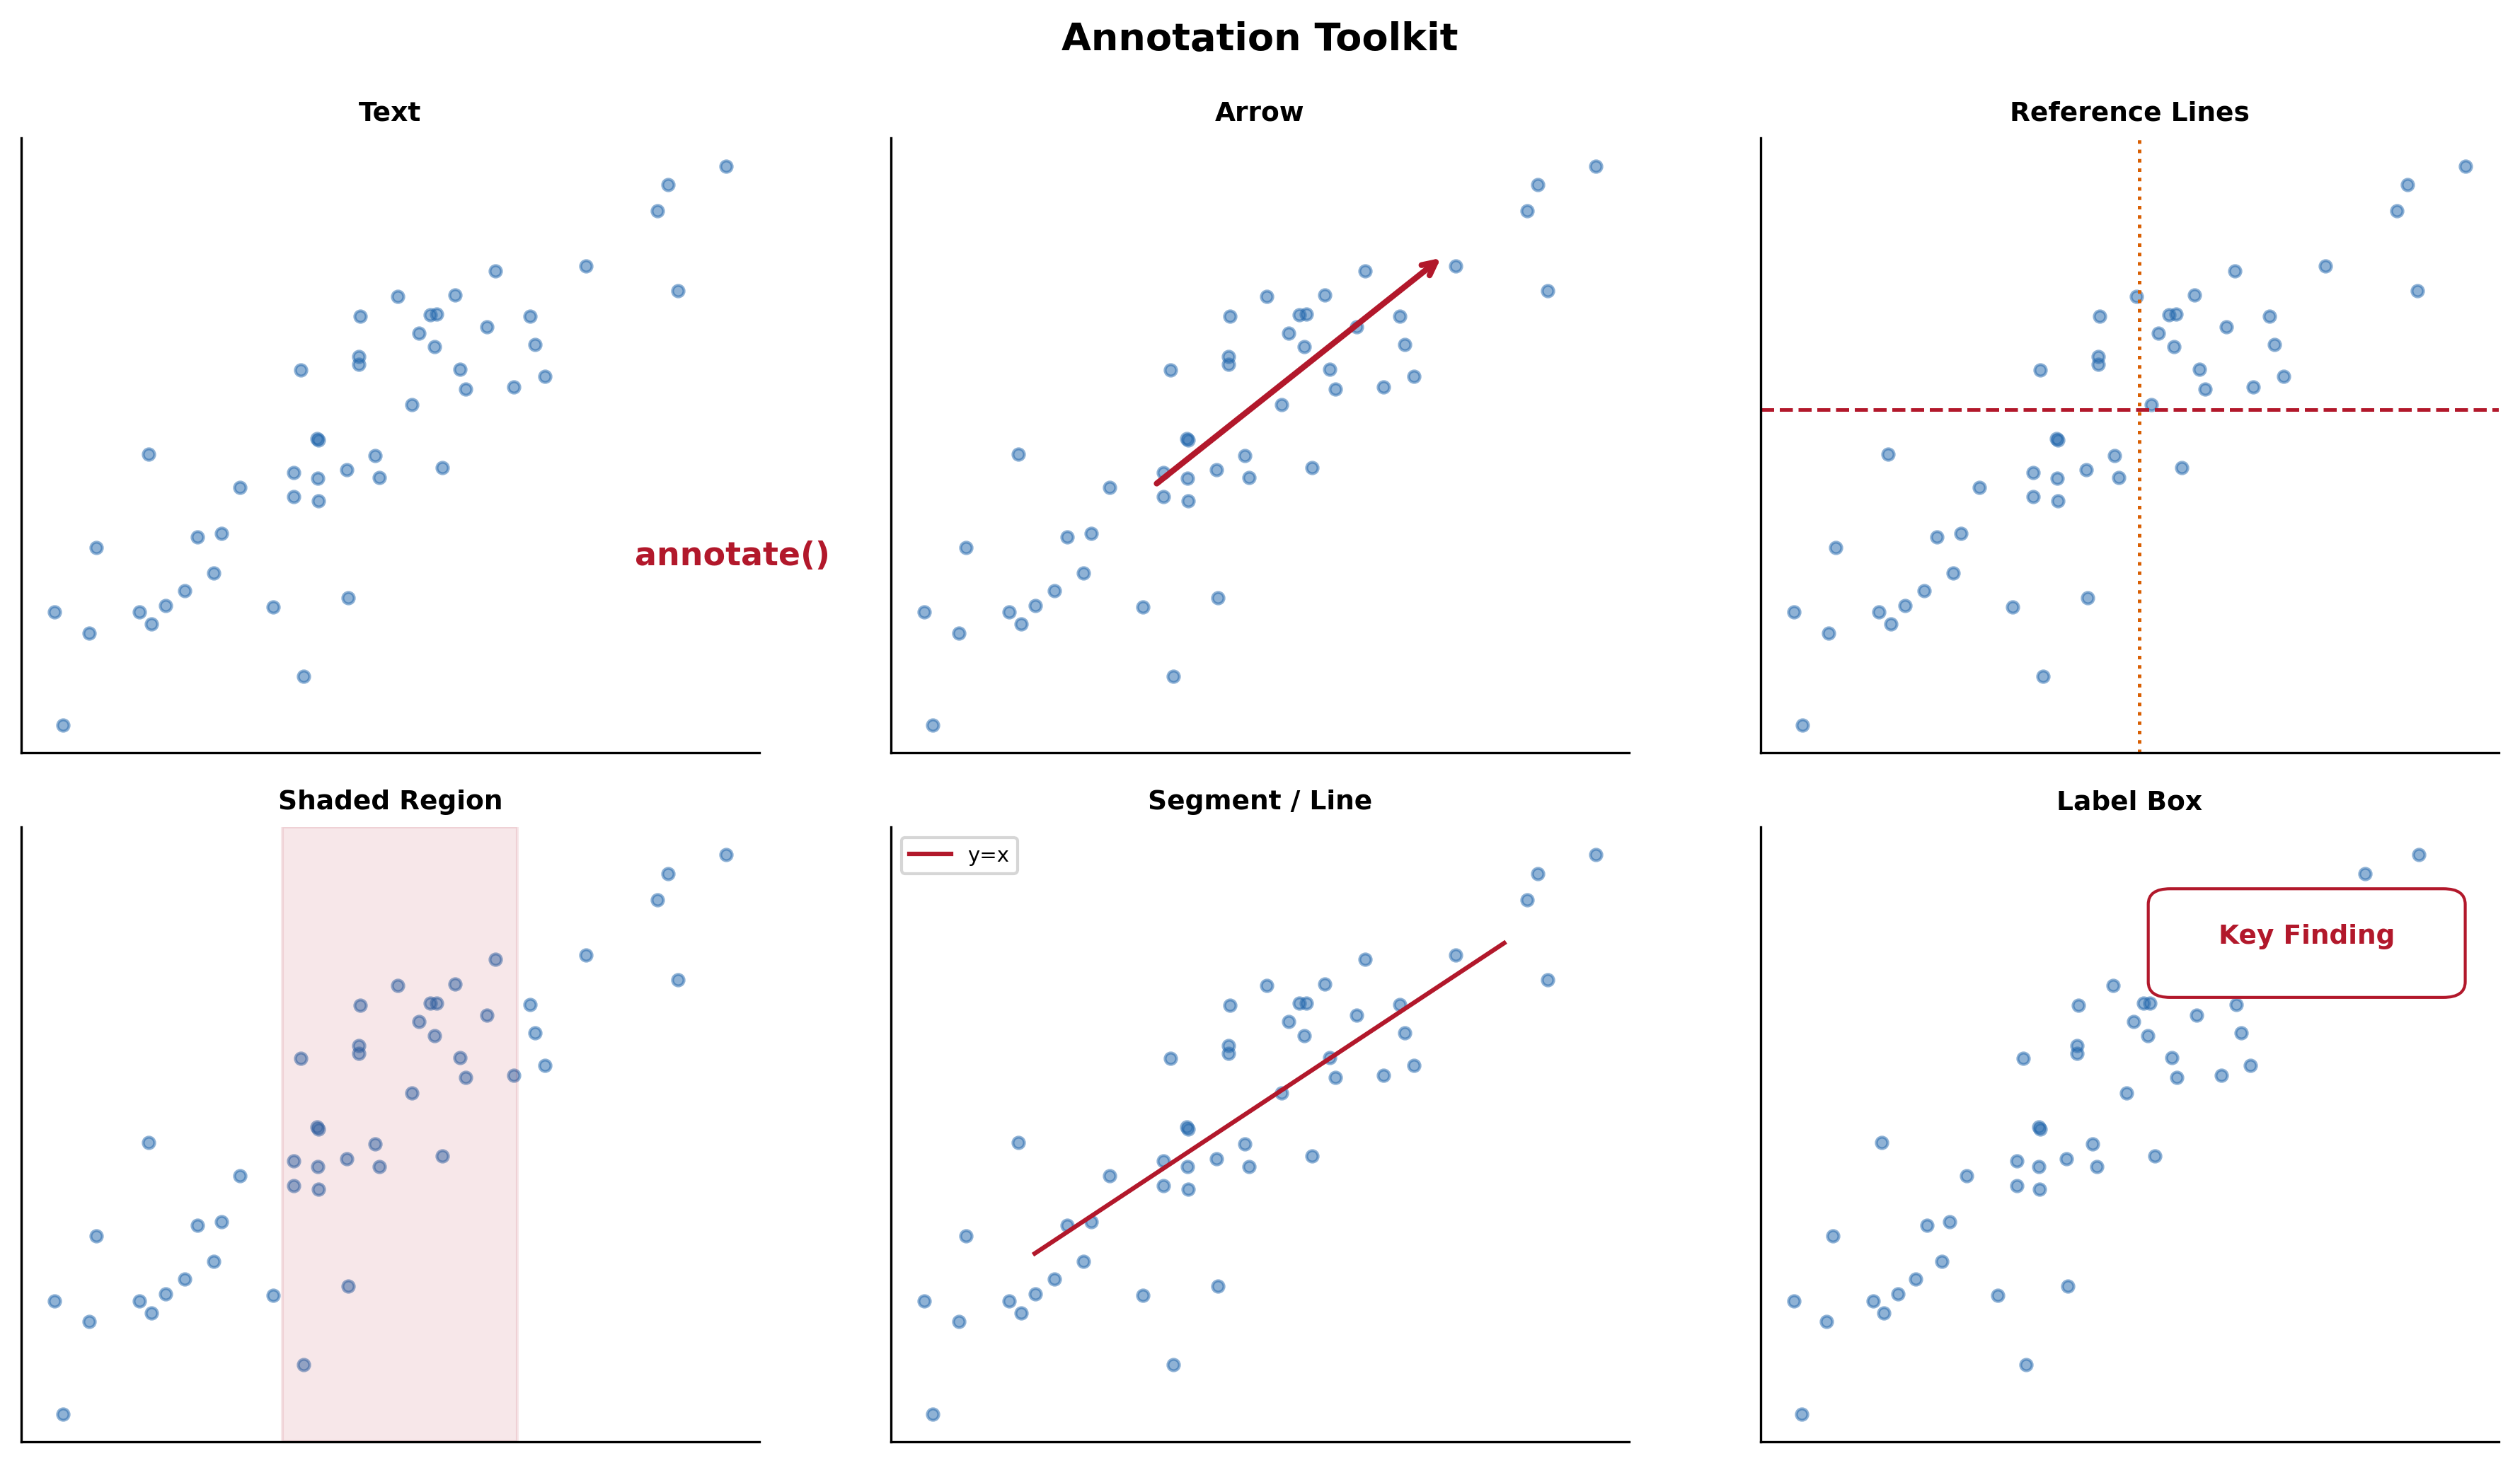
\includegraphics[width=0.88\textwidth]{m1_9_annotation_toolkit.png}

\vspace{0.2cm}
\begin{exampleblock}{Data Insight}
    \scriptsize Six annotation primitives cover 95\% of labeling needs: free text, arrows, reference lines, shaded regions, segments, and label boxes. Every grammar implementation provides all six.
\end{exampleblock}
\end{frame}

% ── 243 ──
\begin{frame}{Why Annotate?}
\smark{243/300}
\begin{columns}[T]
\begin{column}{0.50\textwidth}
\begin{itemize}
    \item Raw charts show \textbf{data}; annotations add \textbf{meaning}
    \item Point out outliers, events, thresholds, trends
    \item Reduce cognitive load: the reader doesn't have to hunt for the message
    \item Knaflic (2015): ``If there is a conclusion you want your audience to reach, state it directly.''
\end{itemize}
\end{column}
\begin{column}{0.47\textwidth}
\begin{alertblock}{Pro-Tip}
    \scriptsize Under-annotated: the reader is lost. Over-annotated: the chart becomes a word cloud. Rule of thumb: \textbf{1--3 annotations} per plot, each one earning its ink.
\end{alertblock}
\vspace{0.2cm}
\begin{exampleblock}{Data Insight}
    \scriptsize Annotations are the \textbf{storytelling layer}. Data + geom + aes tell \emph{what happened}. Annotations tell \emph{what it means}.
\end{exampleblock}
\end{column}
\end{columns}
\end{frame}

% ── 244 ──
\begin{frame}{\texttt{annotate()} vs.\ \texttt{geom\_text()}}
\smark{244/300}
\centering\small
\begin{tabular}{@{}lll@{}}
    \toprule
    \textbf{Feature} & \texttt{annotate()} & \texttt{geom\_text()} \\
    \midrule
    Data source     & Manual coordinates       & Maps from data frame \\
    Use case        & Fixed labels, arrows      & Label every data point \\
    Facets          & Appears in \textbf{all} panels & Respects facet grouping \\
    Scales          & Ignores legend            & Can map to \texttt{aes()} \\
    Typical count   & 1--5 per plot             & $n$ labels (one per row) \\
    \bottomrule
\end{tabular}

\vspace{0.3cm}
\begin{exampleblock}{Data Insight}
    \scriptsize Use \texttt{annotate("text", ...)} for fixed commentary (``recession starts here''). Use \texttt{geom\_text(aes(label=name))} when each point needs its own label from a column.
\end{exampleblock}
\end{frame}

% ── 245 ──
\begin{frame}[fragile]{Text + Arrow Annotation --- \Rlang}\smark{245/300}
\begin{columns}[T]
\begin{column}{0.55\textwidth}
\begin{lstlisting}[style=Rstyle]
ggplot(penguins,
  aes(bill_length_mm,
      body_mass_g,
      color = species)) +
  geom_point(alpha = 0.7) +
  annotate("text",
    x = 55, y = 5500,
    label = "Largest Gentoo",
    fontface = "bold",
    size = 3.5) +
  annotate("segment",
    x = 54.5, y = 5600,
    xend = 49.5, yend = 6250,
    arrow = arrow(length =
      unit(0.2, "cm"))) +
  theme_minimal()
\end{lstlisting}
\end{column}
\begin{column}{0.42\textwidth}
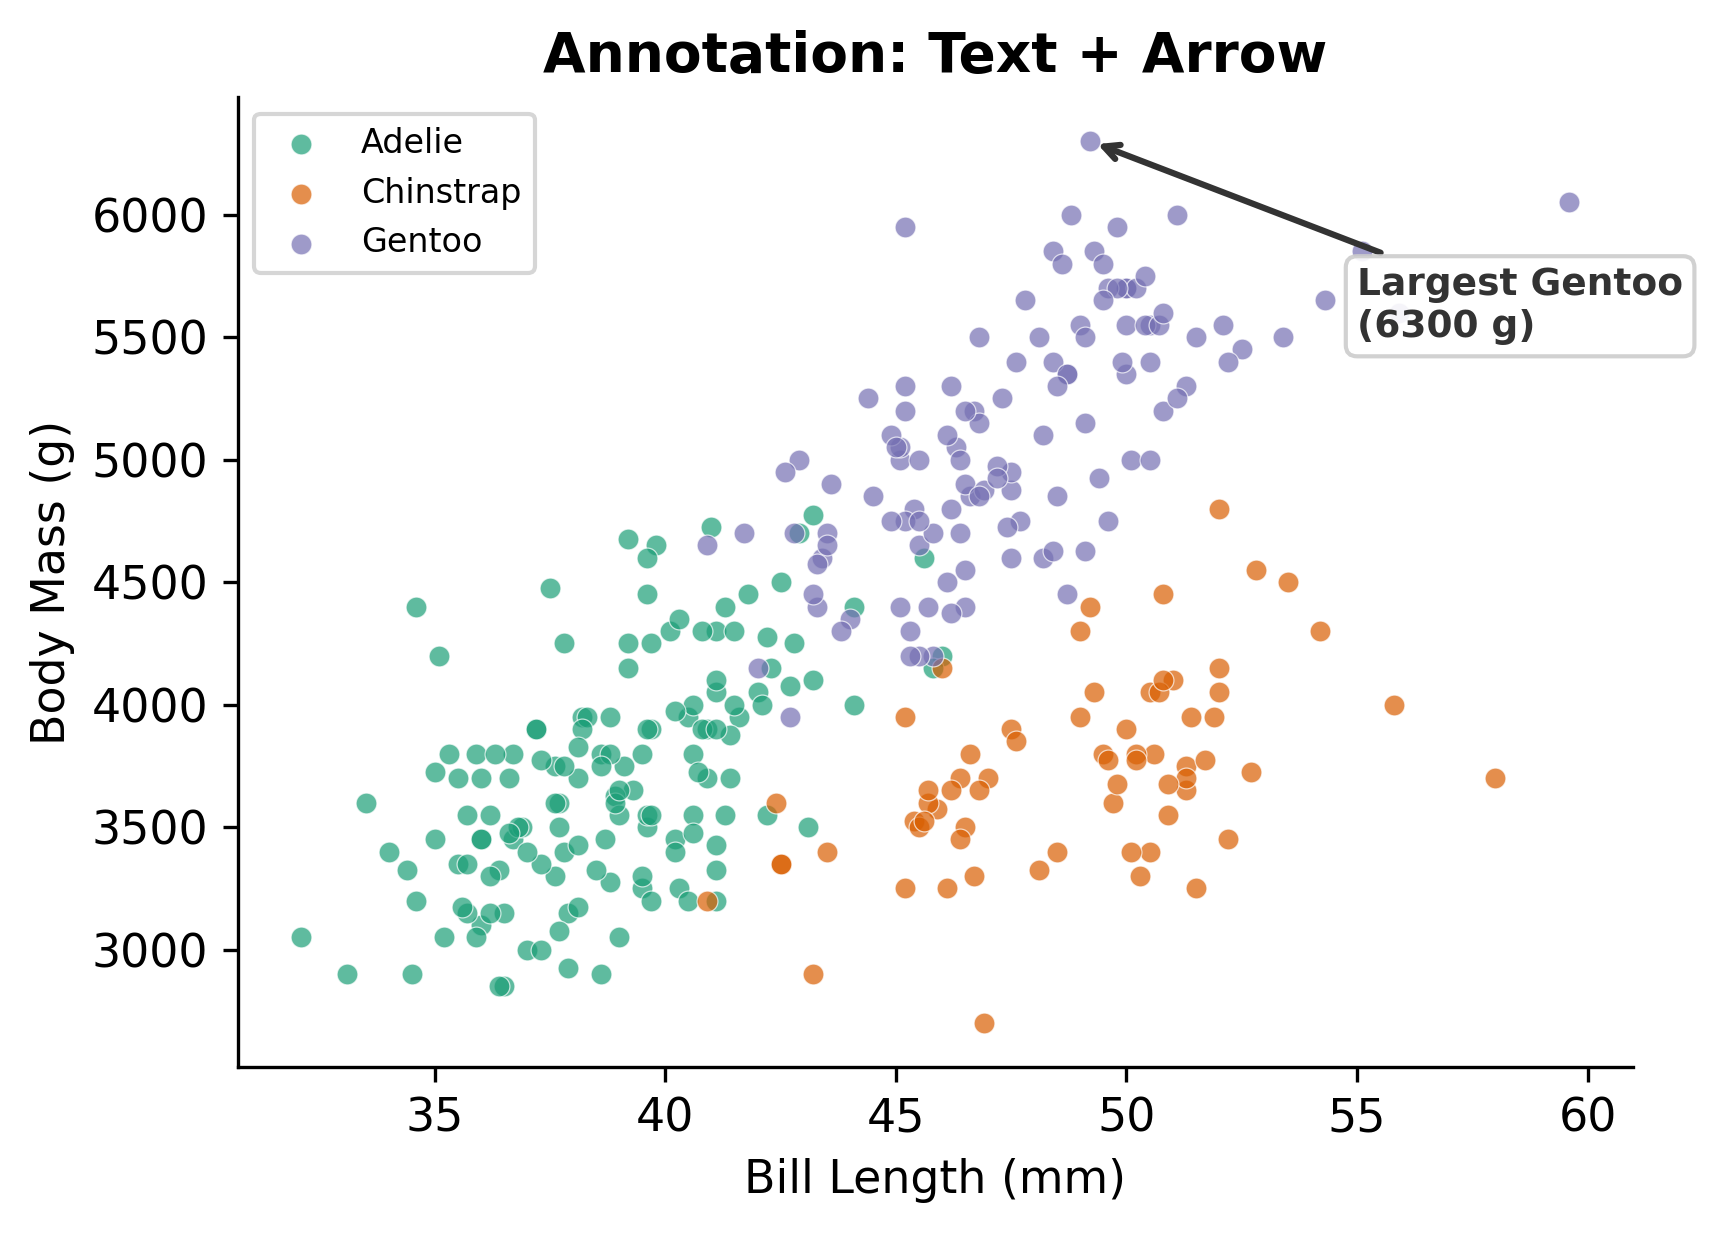
\includegraphics[width=\textwidth]{m1_9_annotate_arrow.png}
\begin{alertblock}{Pro-Tip}
    \scriptsize \texttt{annotate("segment", ..., arrow=arrow())} draws the arrow. Separate \texttt{annotate("text")} places the label. Two calls, one annotation.
\end{alertblock}
\end{column}
\end{columns}
\end{frame}

% ── 246 ──
\begin{frame}[fragile]{Text + Arrow Annotation --- \Python}\smark{246/300}
\begin{columns}[T]
\begin{column}{0.55\textwidth}
\begin{lstlisting}[style=Pystyle]
# matplotlib
ax.annotate(
    "Largest Gentoo\n(6300 g)",
    xy=(49.2, 6300),      # point
    xytext=(55, 5500),     # label
    fontsize=9,
    fontweight="bold",
    arrowprops=dict(
        arrowstyle="->",
        color="#333", lw=1.5),
    bbox=dict(
        boxstyle="round,pad=0.3",
        facecolor="white",
        edgecolor="#CCC"))

# plotnine
(ggplot(...) +
 annotate("text", x=55, y=5500,
          label="Largest Gentoo"))
\end{lstlisting}
\end{column}
\begin{column}{0.42\textwidth}
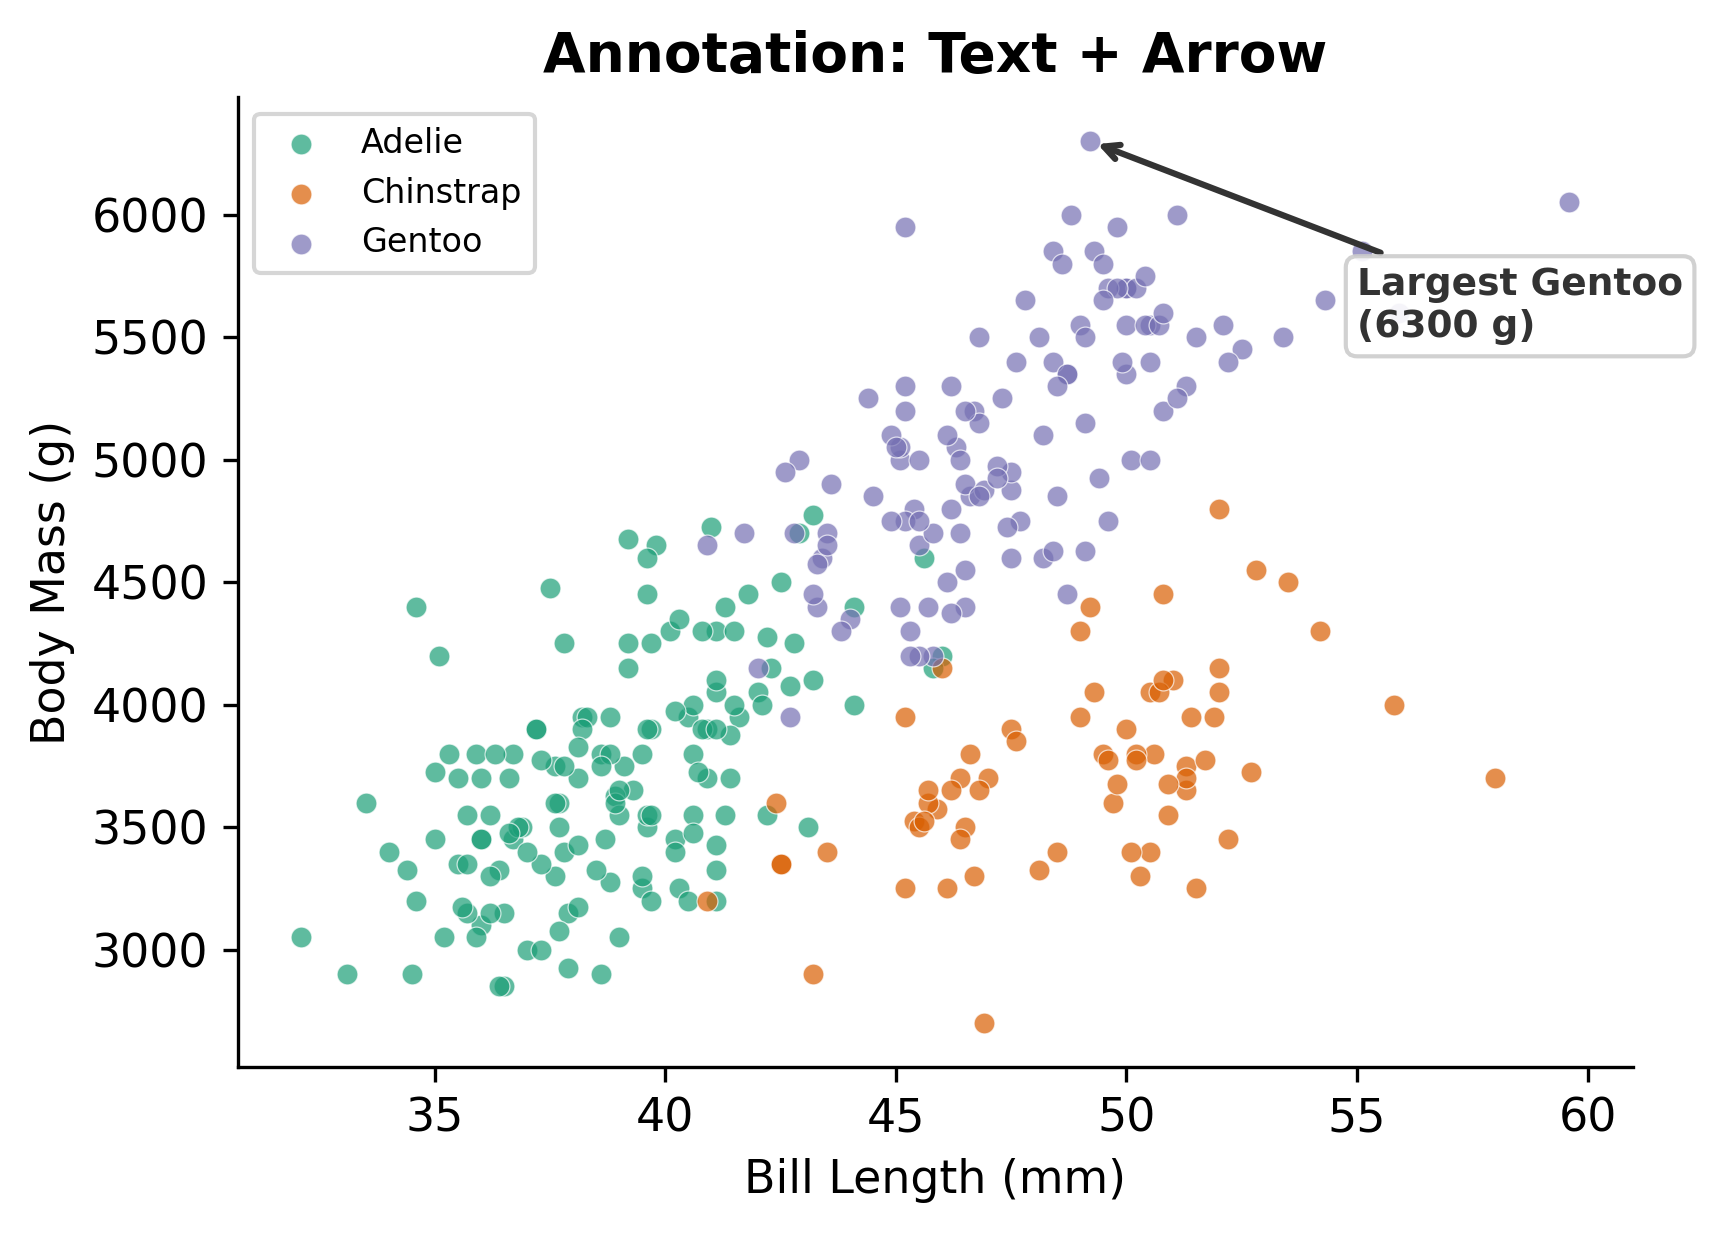
\includegraphics[width=\textwidth]{m1_9_annotate_arrow.png}
\begin{exampleblock}{Data Insight}
    \scriptsize matplotlib's \texttt{ax.annotate()} is more powerful than ggplot2's: it handles text, arrow, and bounding box in one call. ggplot2 requires separate \texttt{annotate()} calls.
\end{exampleblock}
\end{column}
\end{columns}
\end{frame}

% ── 247 ──
\begin{frame}{Reference Lines: hline, vline, abline}
\smark{247/300}
\centering
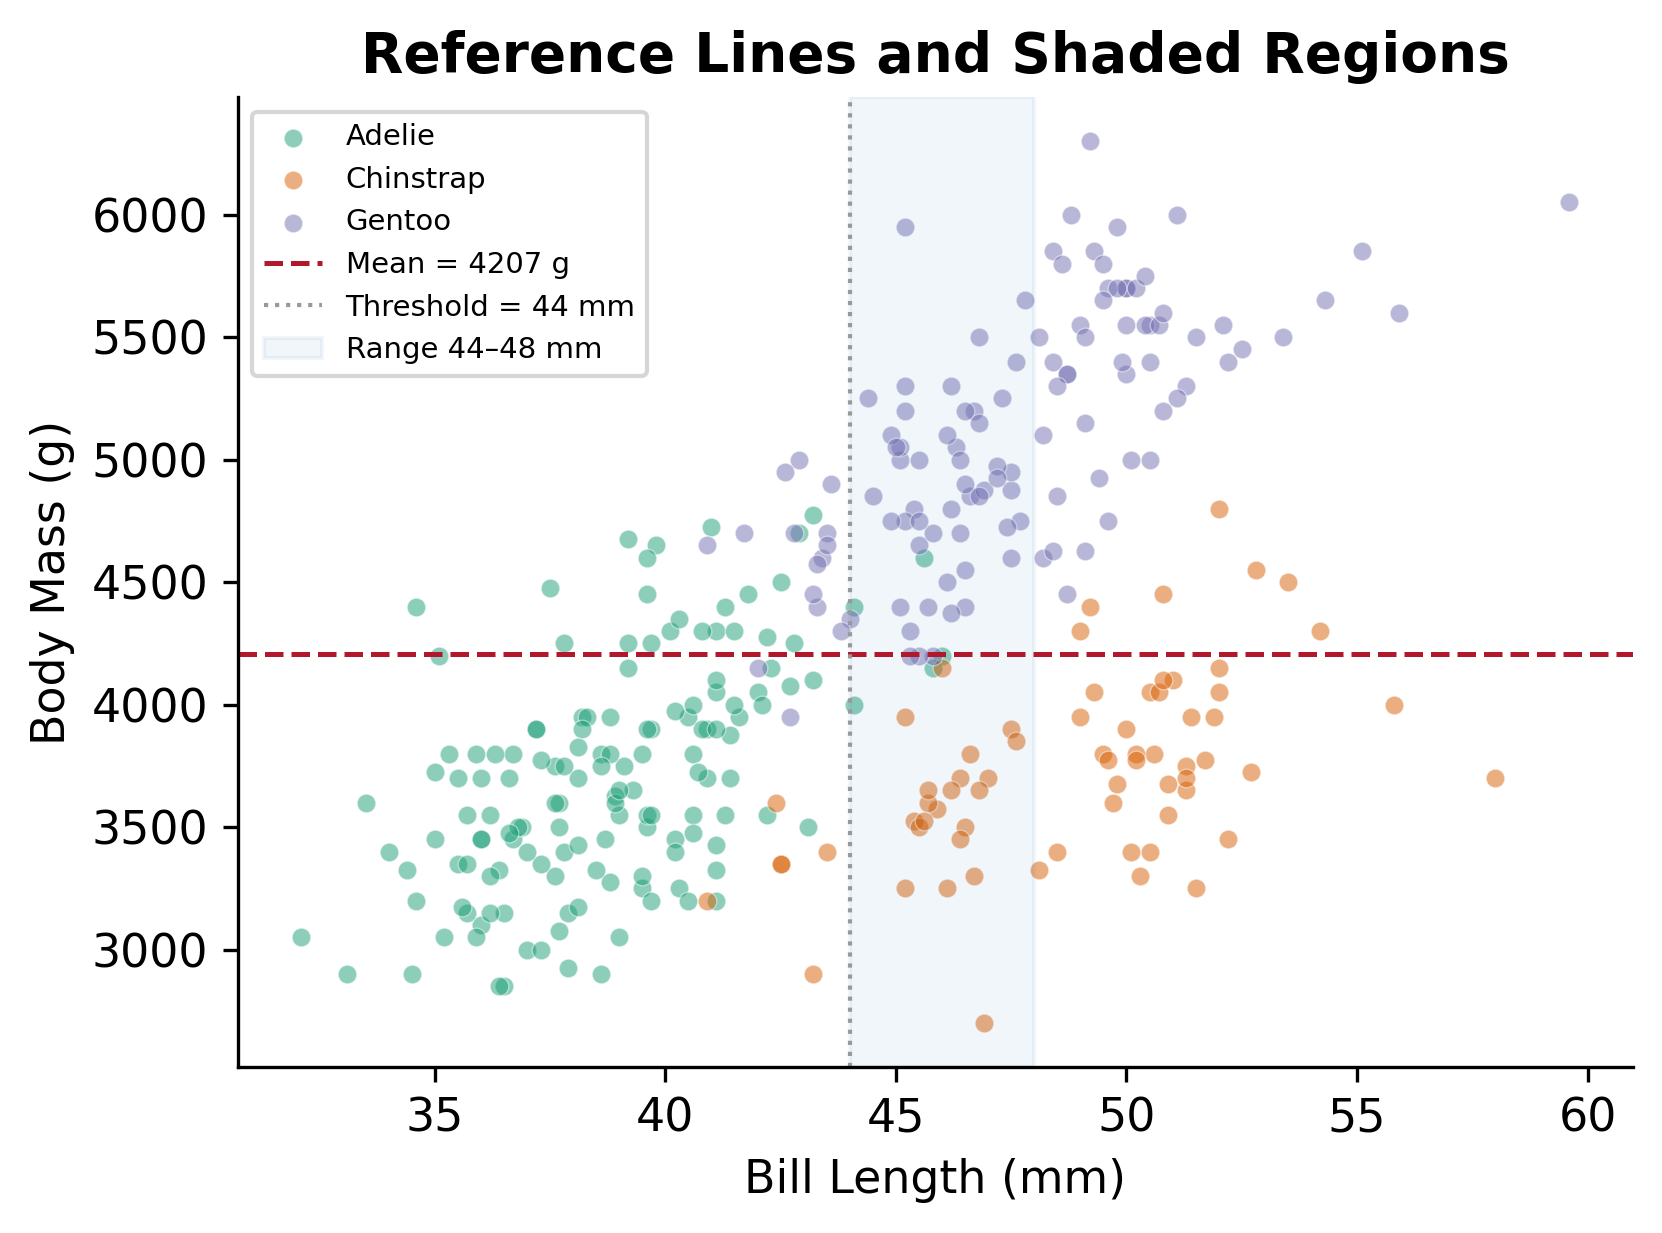
\includegraphics[width=0.72\textwidth]{m1_9_reference_lines.png}

\vspace{0.2cm}
\begin{columns}[T]
\begin{column}{0.48\textwidth}
\begin{itemize}
    \item \textbf{hline}: horizontal threshold (mean, target, regulation limit)
    \item \textbf{vline}: vertical event marker (date, cutoff)
    \item \textbf{abline}: diagonal reference ($y = x$, regression)
\end{itemize}
\end{column}
\begin{column}{0.48\textwidth}
\begin{alertblock}{Pro-Tip}
    \scriptsize Use dashed or dotted lines for references (they are \emph{not} data). Solid lines are reserved for data traces.
\end{alertblock}
\end{column}
\end{columns}
\end{frame}

% ── 248 ──
\begin{frame}[fragile]{Reference Lines --- Code}\smark{248/300}
\begin{columns}[T]
\begin{column}{0.48\textwidth}
\begin{lstlisting}[style=Rstyle]
ggplot(penguins, aes(...)) +
  geom_point() +
  # Horizontal mean
  geom_hline(
    yintercept = mean(
      penguins$body_mass_g),
    linetype = "dashed",
    color = "#B2182B") +
  # Vertical threshold
  geom_vline(xintercept = 44,
    linetype = "dotted") +
  # Shaded range
  annotate("rect",
    xmin=44, xmax=48,
    ymin=-Inf, ymax=Inf,
    alpha=0.06, fill="#2166AC")
\end{lstlisting}
\end{column}
\begin{column}{0.48\textwidth}
\begin{lstlisting}[style=Pystyle]
# matplotlib
ax.axhline(y=mean_mass,
    linestyle="--", color="#B2182B")
ax.axvline(x=44,
    linestyle=":", color="#999")
ax.axvspan(44, 48,
    alpha=0.06, color="#2166AC")

# plotnine
(ggplot(...) +
 geom_hline(yintercept=mean_mass,
    linetype="dashed",
    color="#B2182B") +
 geom_vline(xintercept=44,
    linetype="dotted"))
\end{lstlisting}
\end{column}
\end{columns}
\end{frame}

% ── 249 ──
\begin{frame}{Shaded Regions for Events and Thresholds}
\smark{249/300}
\centering
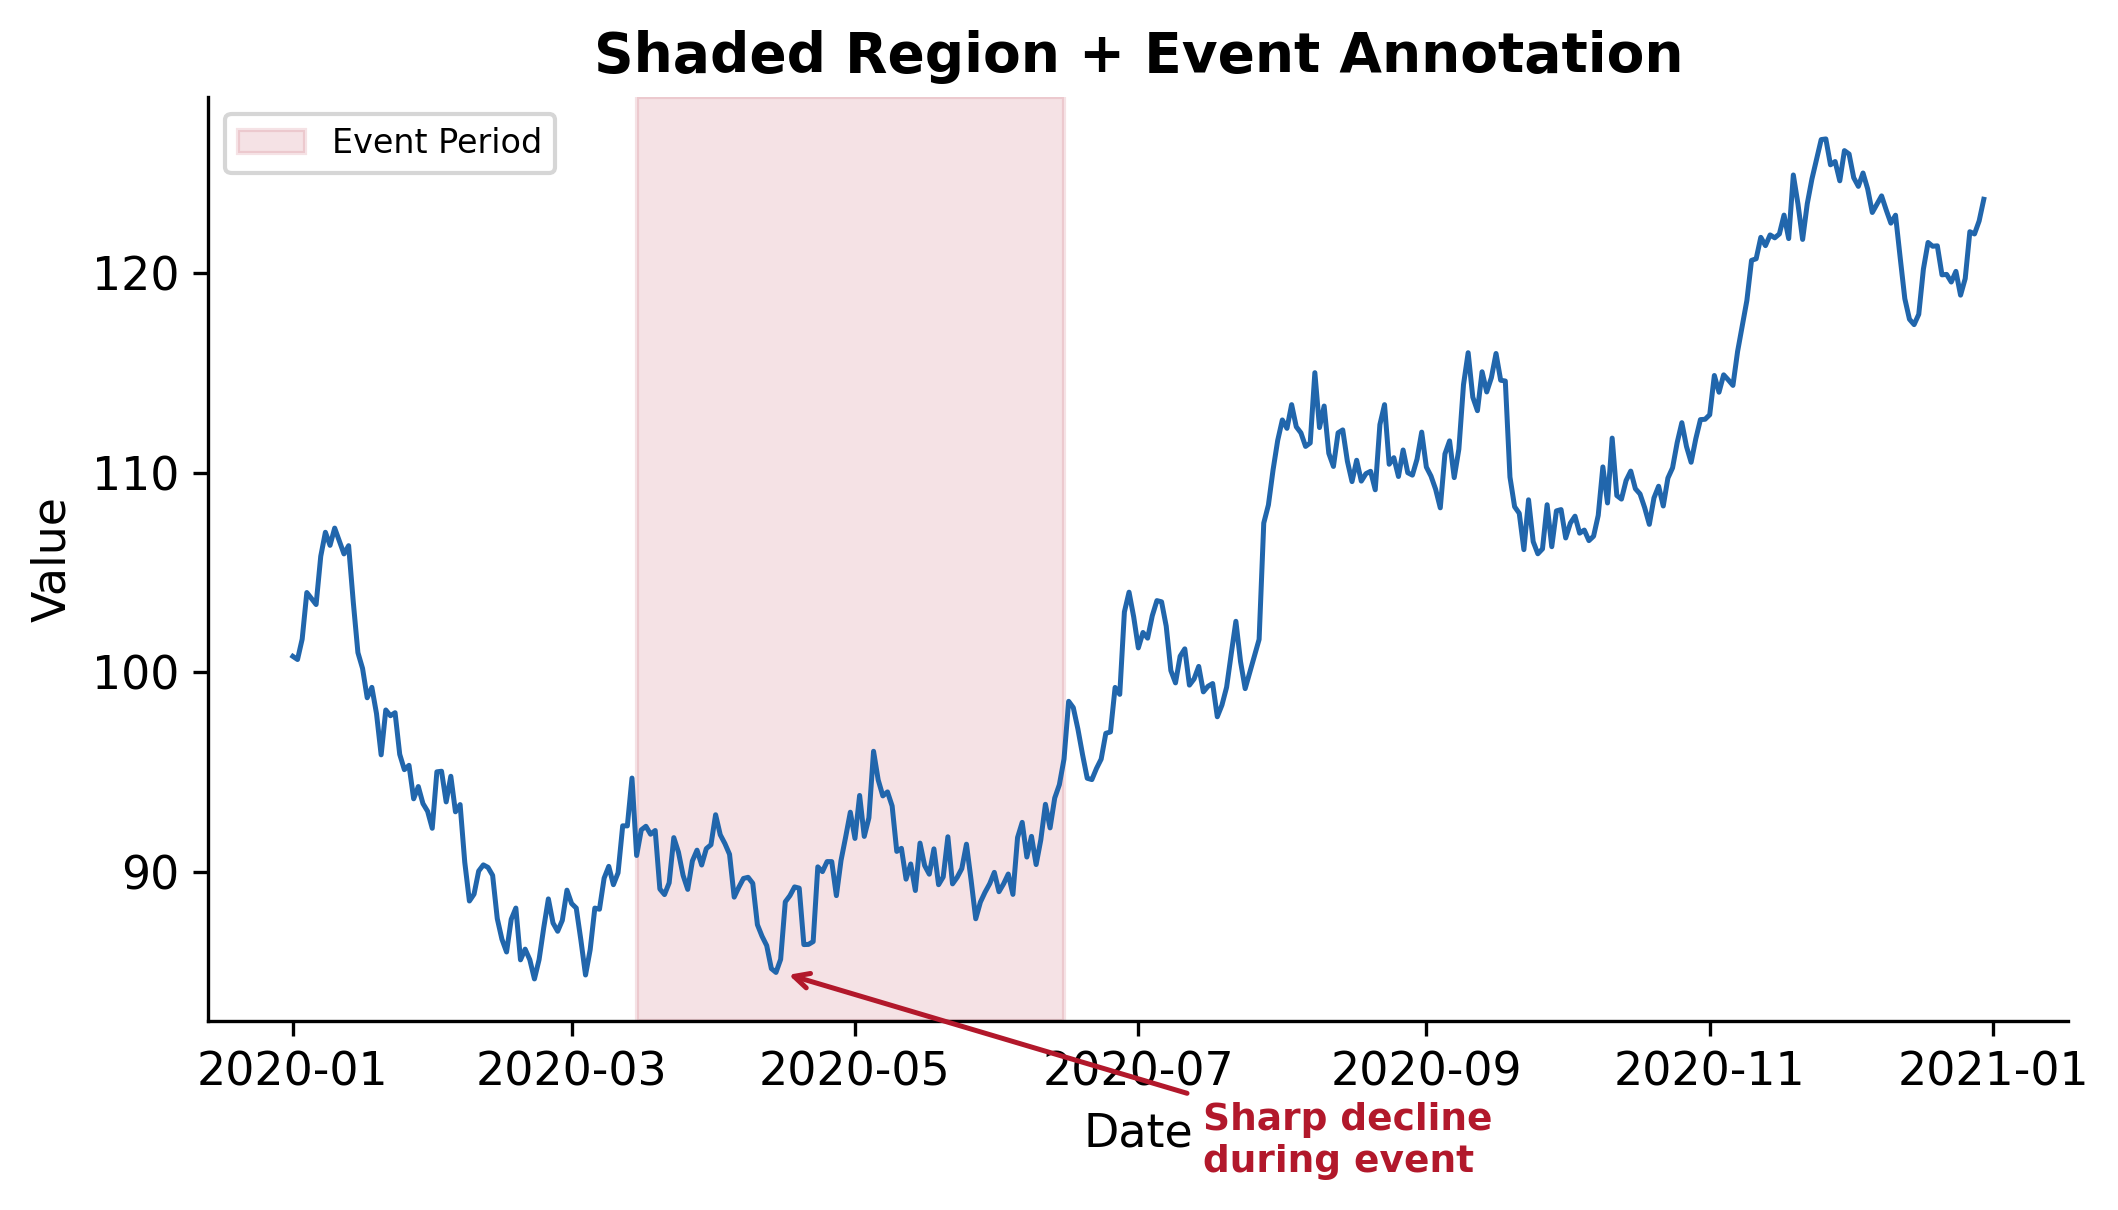
\includegraphics[width=0.78\textwidth]{m1_9_shaded_event.png}

\vspace{0.2cm}
\begin{exampleblock}{Data Insight}
    \scriptsize A shaded band marks an event period (policy change, recession, experiment window). Combined with a text annotation, the reader immediately connects the visual pattern to the cause.
\end{exampleblock}
\end{frame}

% ── 250 ──
\begin{frame}[fragile]{Shaded Events --- Code}\smark{250/300}
\begin{columns}[T]
\begin{column}{0.48\textwidth}
\begin{lstlisting}[style=Rstyle]
ggplot(df, aes(date, value)) +
  geom_line(color="#2166AC") +
  # Shaded event period
  annotate("rect",
    xmin=as.Date("2020-03-15"),
    xmax=as.Date("2020-06-15"),
    ymin=-Inf, ymax=Inf,
    alpha=0.1, fill="#B2182B")+
  # Event label
  annotate("text",
    x=as.Date("2020-04-15"),
    y=max(df$value),
    label="Event Period",
    color="#B2182B",
    fontface="bold", size=3.5)
\end{lstlisting}
\end{column}
\begin{column}{0.48\textwidth}
\begin{lstlisting}[style=Pystyle]
ax.plot(dates, values,
        color="#2166AC")

# Shaded event
ax.axvspan(
    pd.Timestamp("2020-03-15"),
    pd.Timestamp("2020-06-15"),
    alpha=0.1, color="#B2182B")

# Label
ax.annotate("Event Period",
    xy=(pd.Timestamp("2020-04-15"),
        max(values)),
    fontsize=9, color="#B2182B",
    fontweight="bold")
\end{lstlisting}
\end{column}
\end{columns}
\end{frame}

% ── 251 ──
\begin{frame}{Direct Labeling vs.\ Legends}
\smark{251/300}
\centering
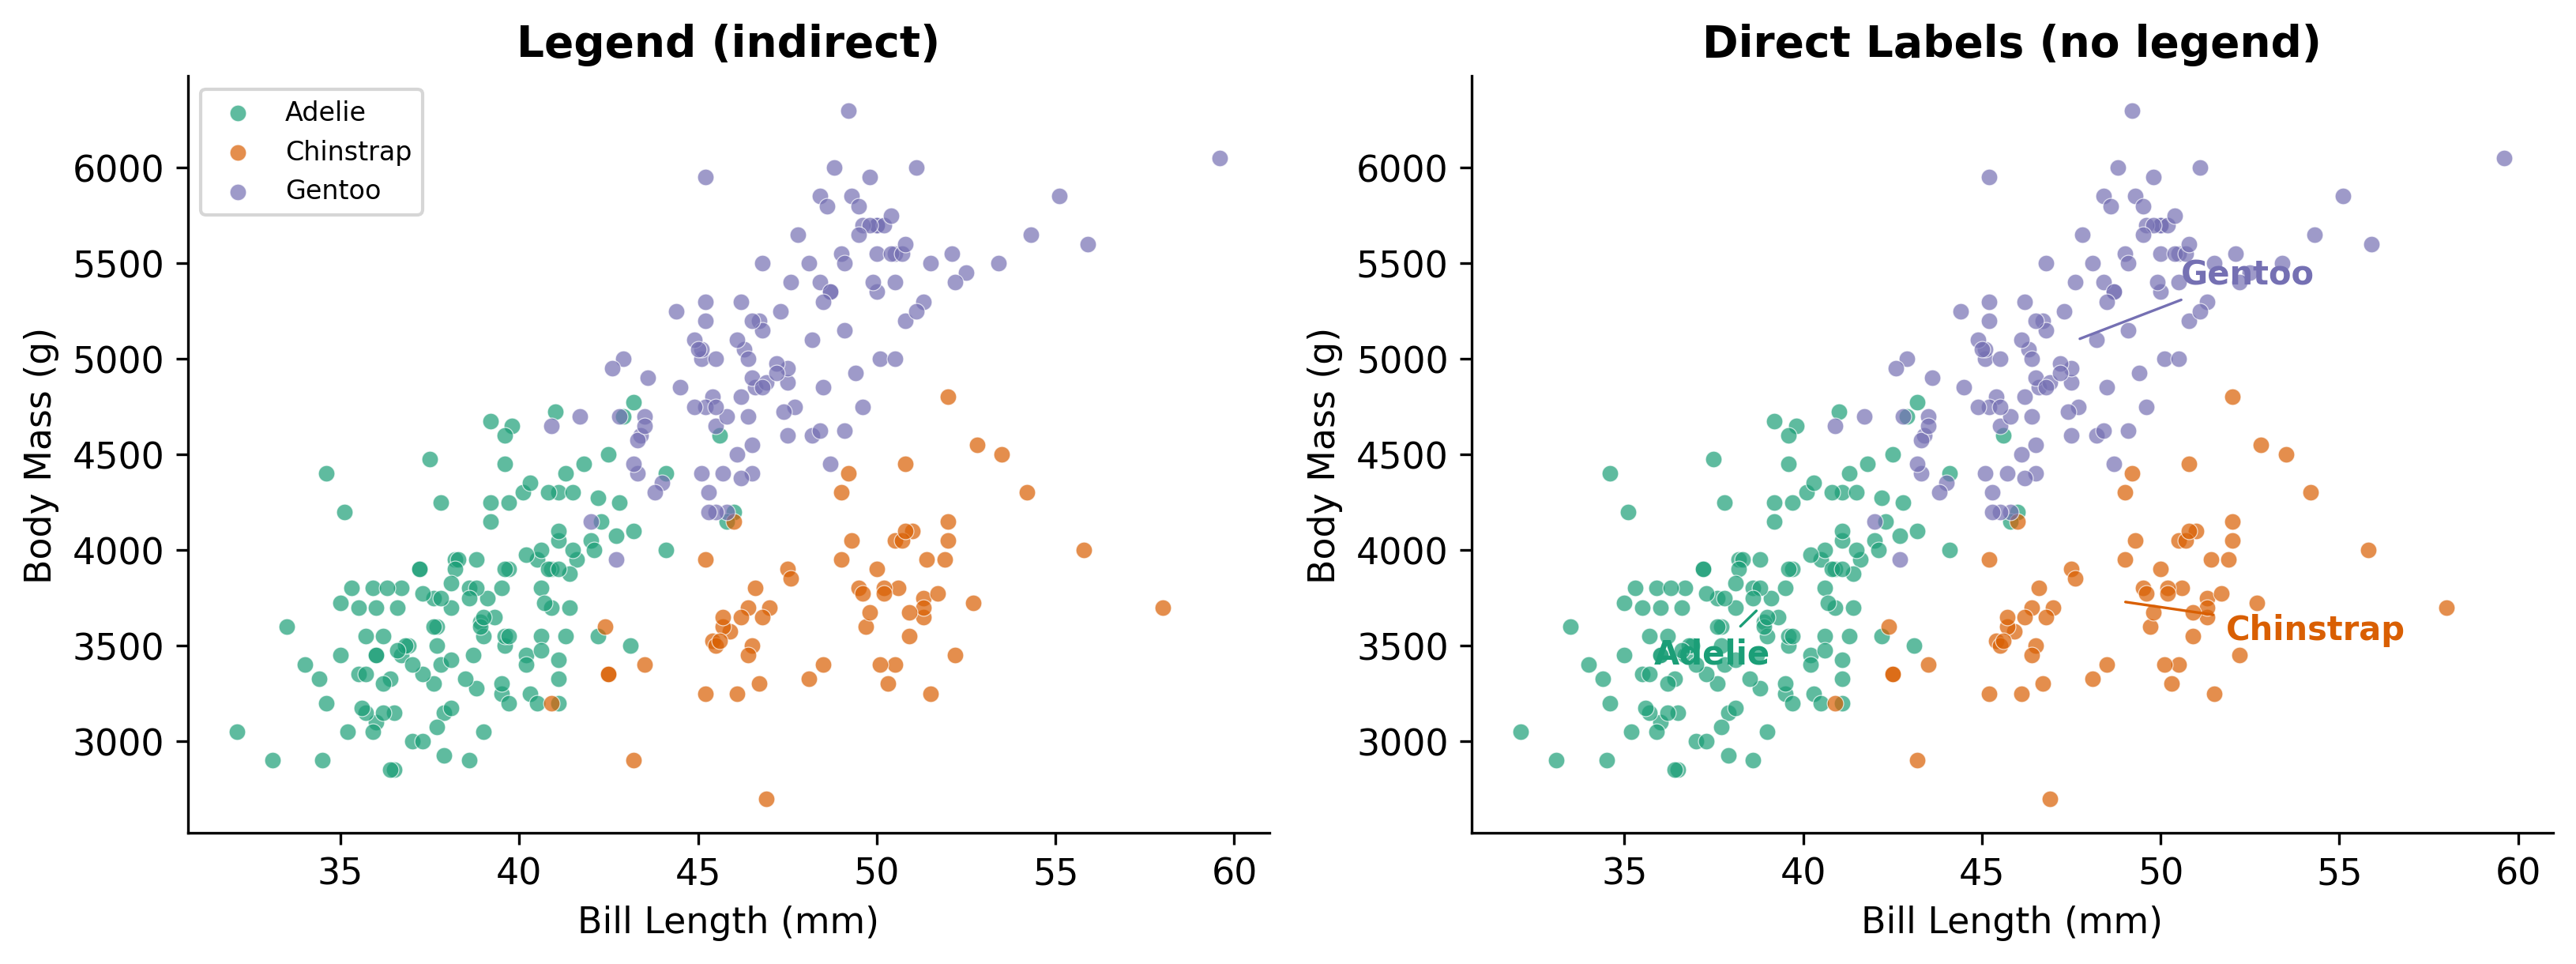
\includegraphics[width=0.88\textwidth]{m1_9_direct_label.png}

\vspace{0.2cm}
\begin{columns}[T]
\begin{column}{0.48\textwidth}
\begin{exampleblock}{Data Insight}
    \scriptsize Left: legend forces the reader to look back and forth between plot and key. Right: labels sit \textbf{next to the data}, eliminating the legend entirely. Knaflic (2015): ``eliminate the legend.''
\end{exampleblock}
\end{column}
\begin{column}{0.48\textwidth}
\begin{alertblock}{Pro-Tip}
    \scriptsize Direct labels work for 2--5 groups. For more, the labels themselves create clutter. Fall back to legend or use faceting.
\end{alertblock}
\end{column}
\end{columns}
\end{frame}

% ── 252 ──
\begin{frame}[fragile]{Direct Labeling --- \Rlang}\smark{252/300}
\begin{columns}[T]
\begin{column}{0.55\textwidth}
\begin{lstlisting}[style=Rstyle]
library(ggrepel)

# Label at group centroid
centroids <- penguins |>
  group_by(species) |>
  summarise(
    x = mean(bill_length_mm),
    y = mean(body_mass_g))

ggplot(penguins, aes(
    bill_length_mm, body_mass_g,
    color=species)) +
  geom_point(alpha=0.6) +
  geom_label_repel(
    data = centroids,
    aes(x, y, label=species),
    size=3.5, fontface="bold",
    show.legend=FALSE) +
  theme(legend.position="none")
\end{lstlisting}
\end{column}
\begin{column}{0.42\textwidth}
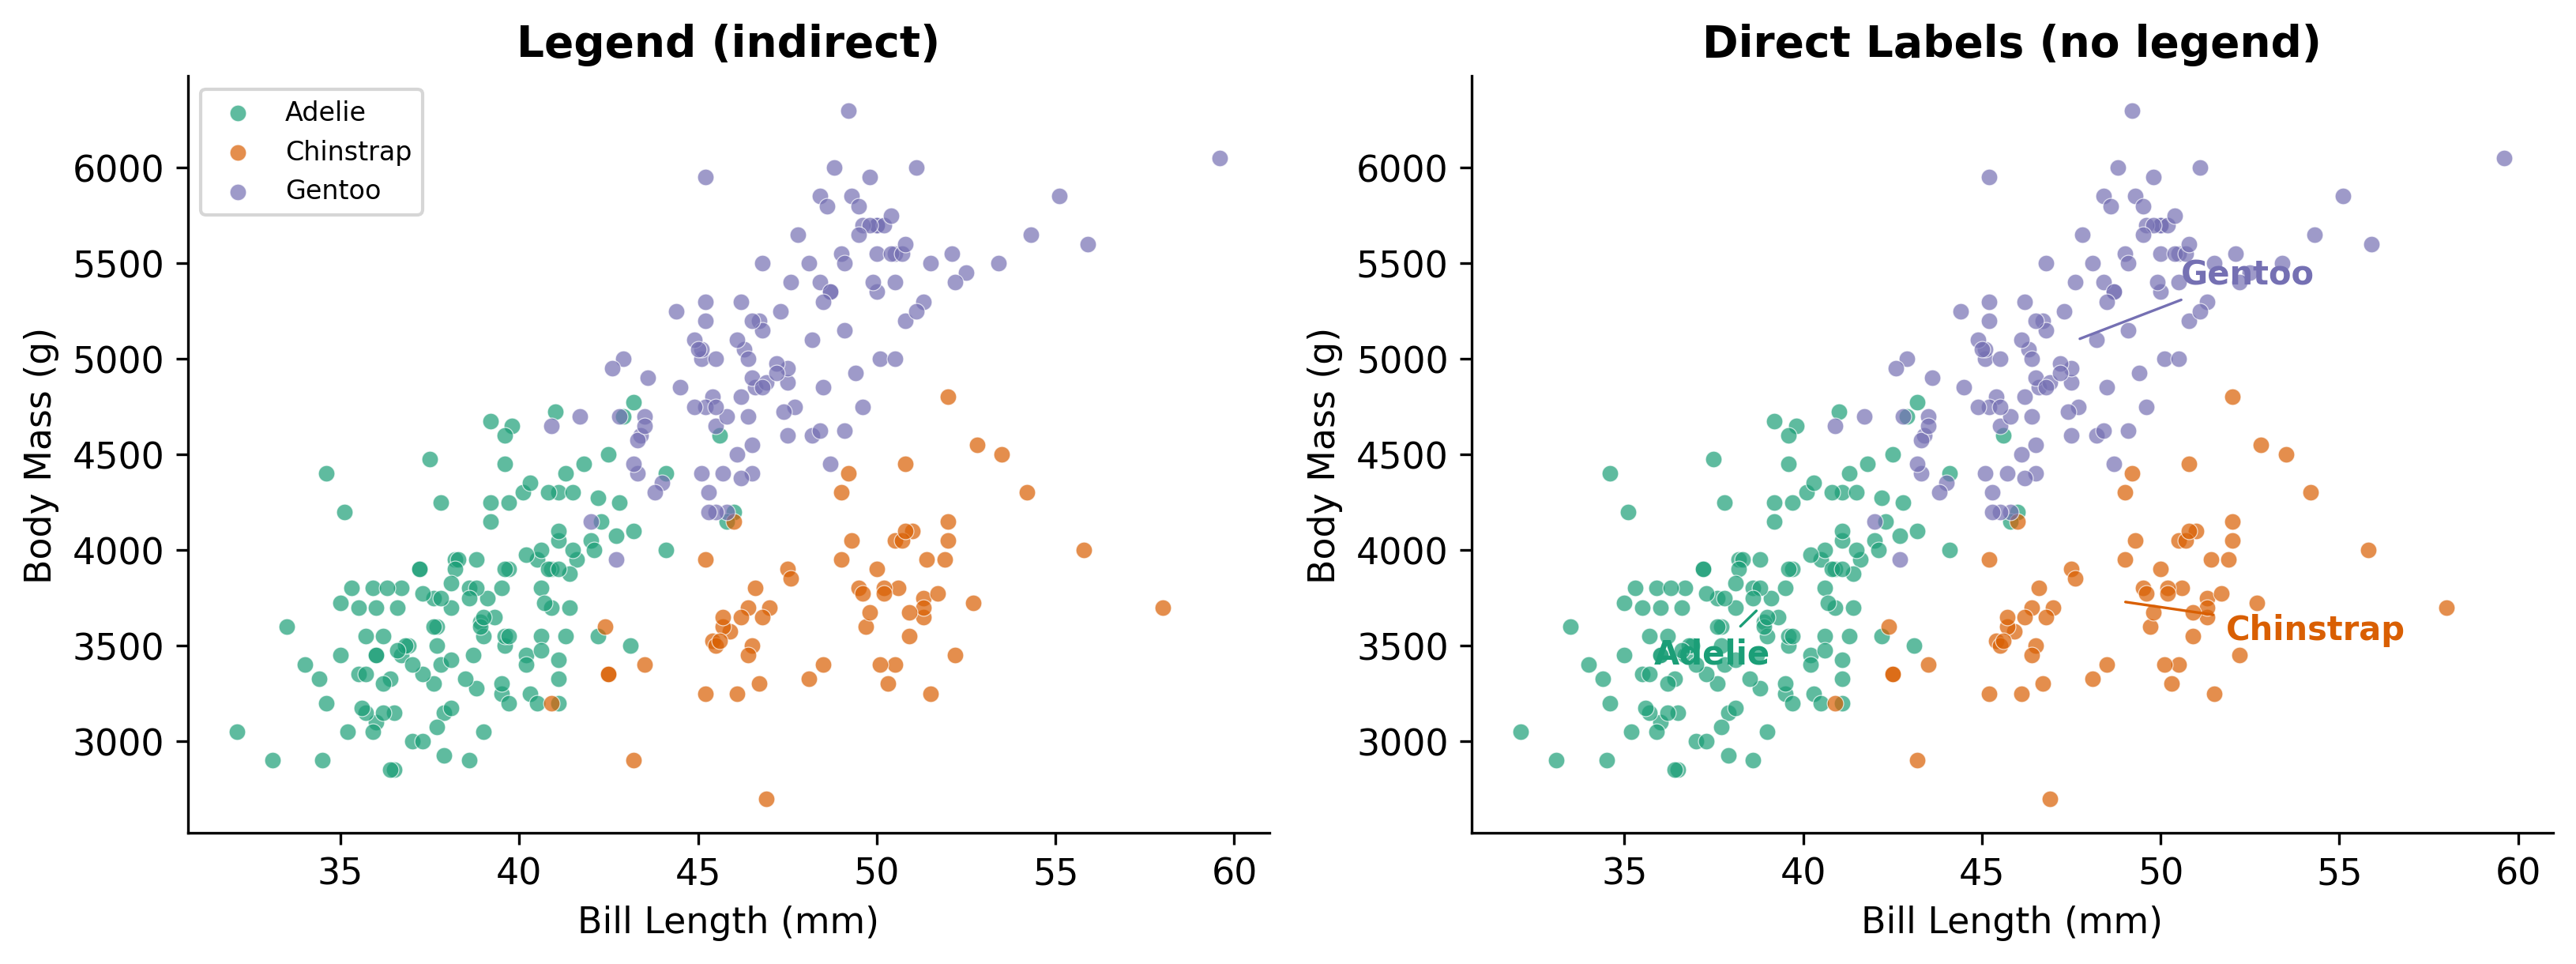
\includegraphics[width=\textwidth]{m1_9_direct_label.png}
\begin{alertblock}{Pro-Tip}
    \scriptsize \texttt{ggrepel} auto-avoids overlap. Compute centroids first, then label at the centroid --- not at every point.
\end{alertblock}
\end{column}
\end{columns}
\end{frame}

% ── 253 ──
\begin{frame}[fragile]{Direct Labeling --- \Python}\smark{253/300}
\begin{columns}[T]
\begin{column}{0.55\textwidth}
\begin{lstlisting}[style=Pystyle]
# Centroids
centroids = pen.groupby("species")[
    ["bill_length_mm",
     "body_mass_g"]].mean()

# matplotlib annotate per group
for sp, c in sc.items():
    cx = centroids.loc[sp,
        "bill_length_mm"]
    cy = centroids.loc[sp,
        "body_mass_g"]
    ax.annotate(sp, xy=(cx, cy),
        fontsize=10, color=c,
        fontweight="bold",
        arrowprops=dict(
            arrowstyle="-",
            color=c, lw=0.8))

# adjustText (pip install)
from adjustText import adjust_text
texts = [ax.text(cx, cy, sp)]
adjust_text(texts)
\end{lstlisting}
\end{column}
\begin{column}{0.42\textwidth}
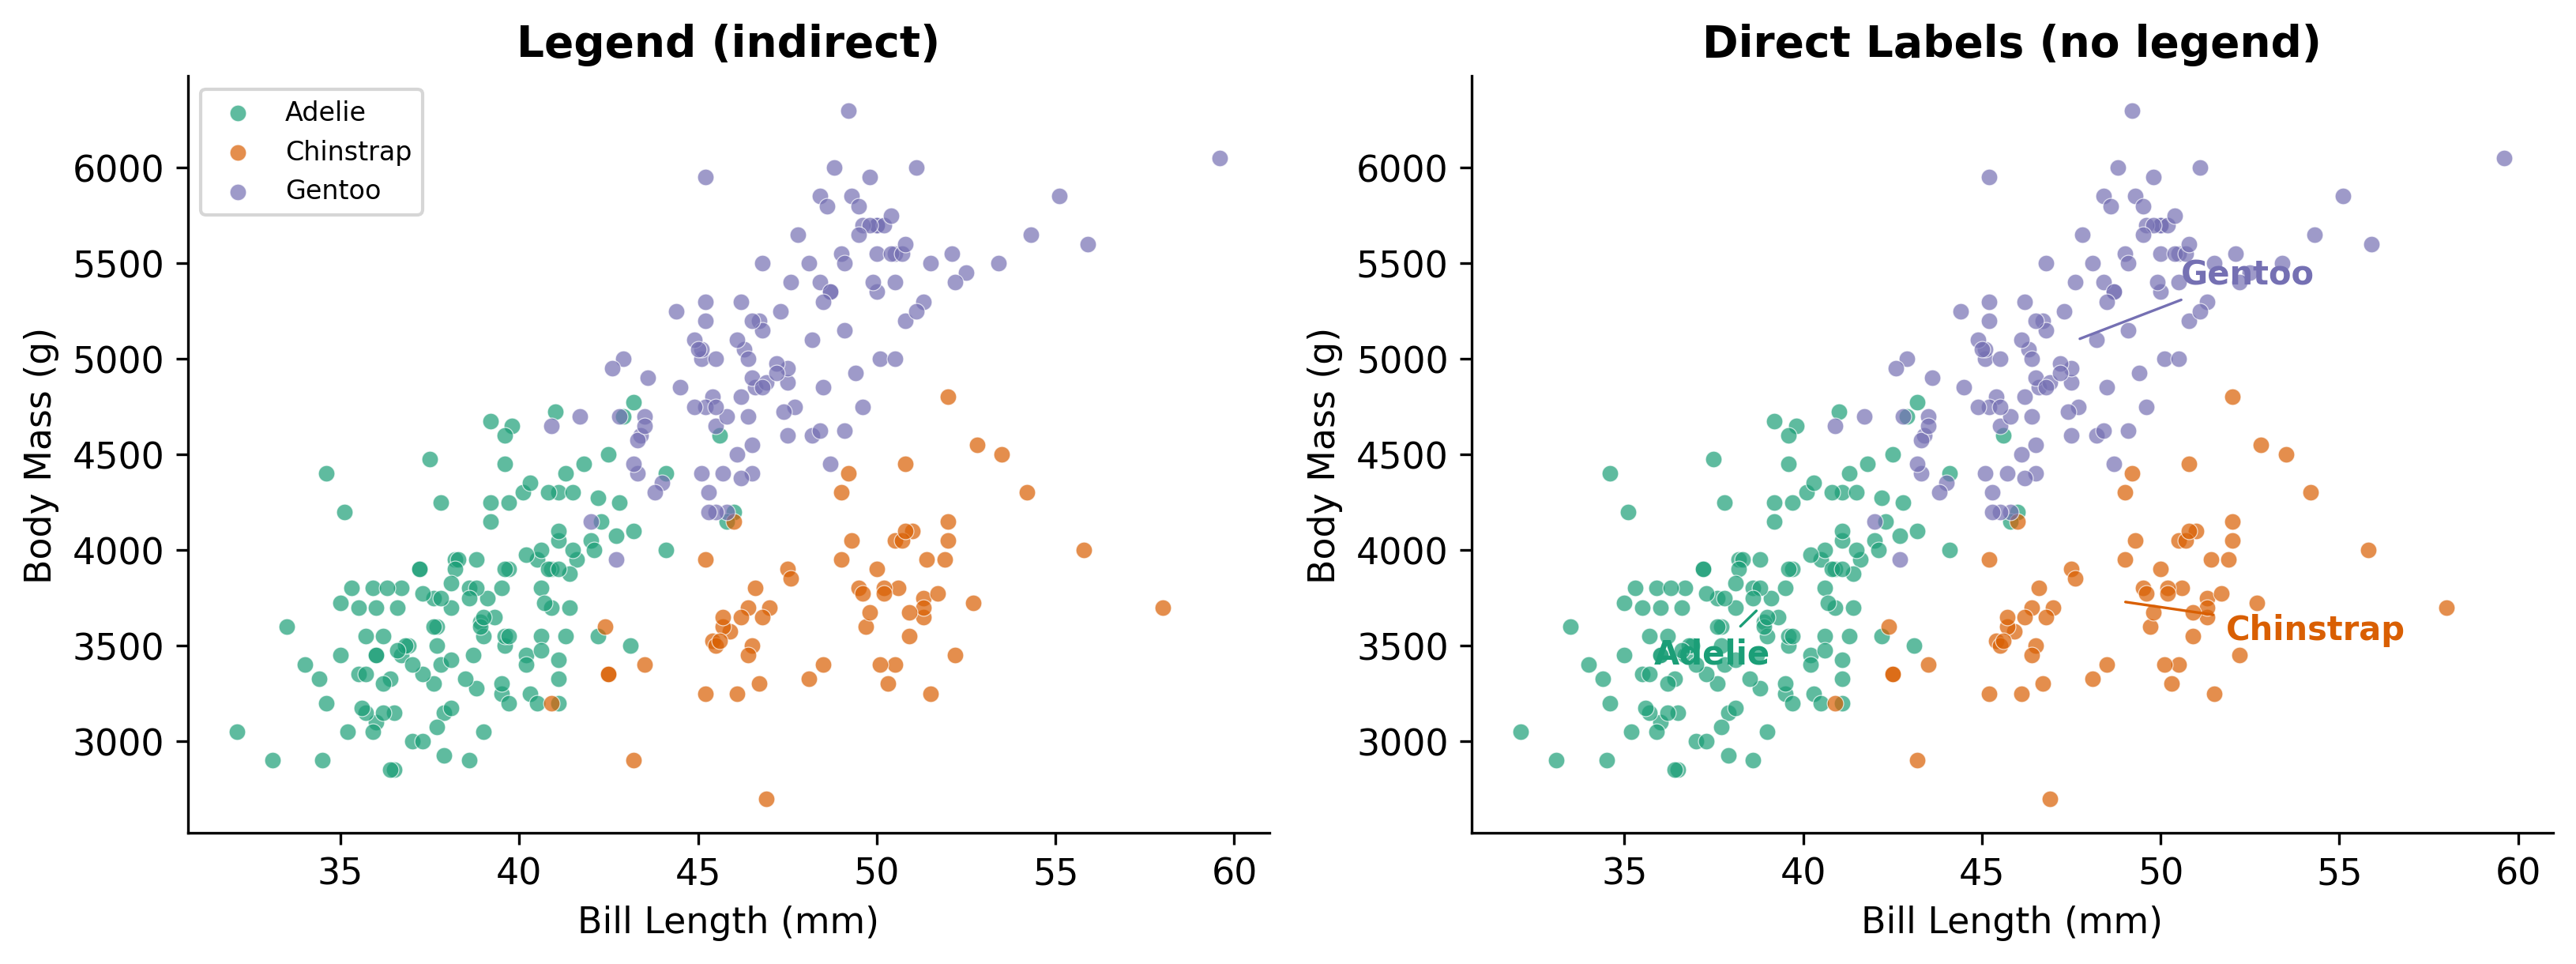
\includegraphics[width=\textwidth]{m1_9_direct_label.png}
\begin{exampleblock}{Data Insight}
    \scriptsize \texttt{adjustText} is the Python equivalent of \texttt{ggrepel}: it iteratively moves text labels to avoid overlap.
\end{exampleblock}
\end{column}
\end{columns}
\end{frame}

% ── 254 ──
\begin{frame}{Titles as Analytical Claims}
\smark{254/300}
\centering
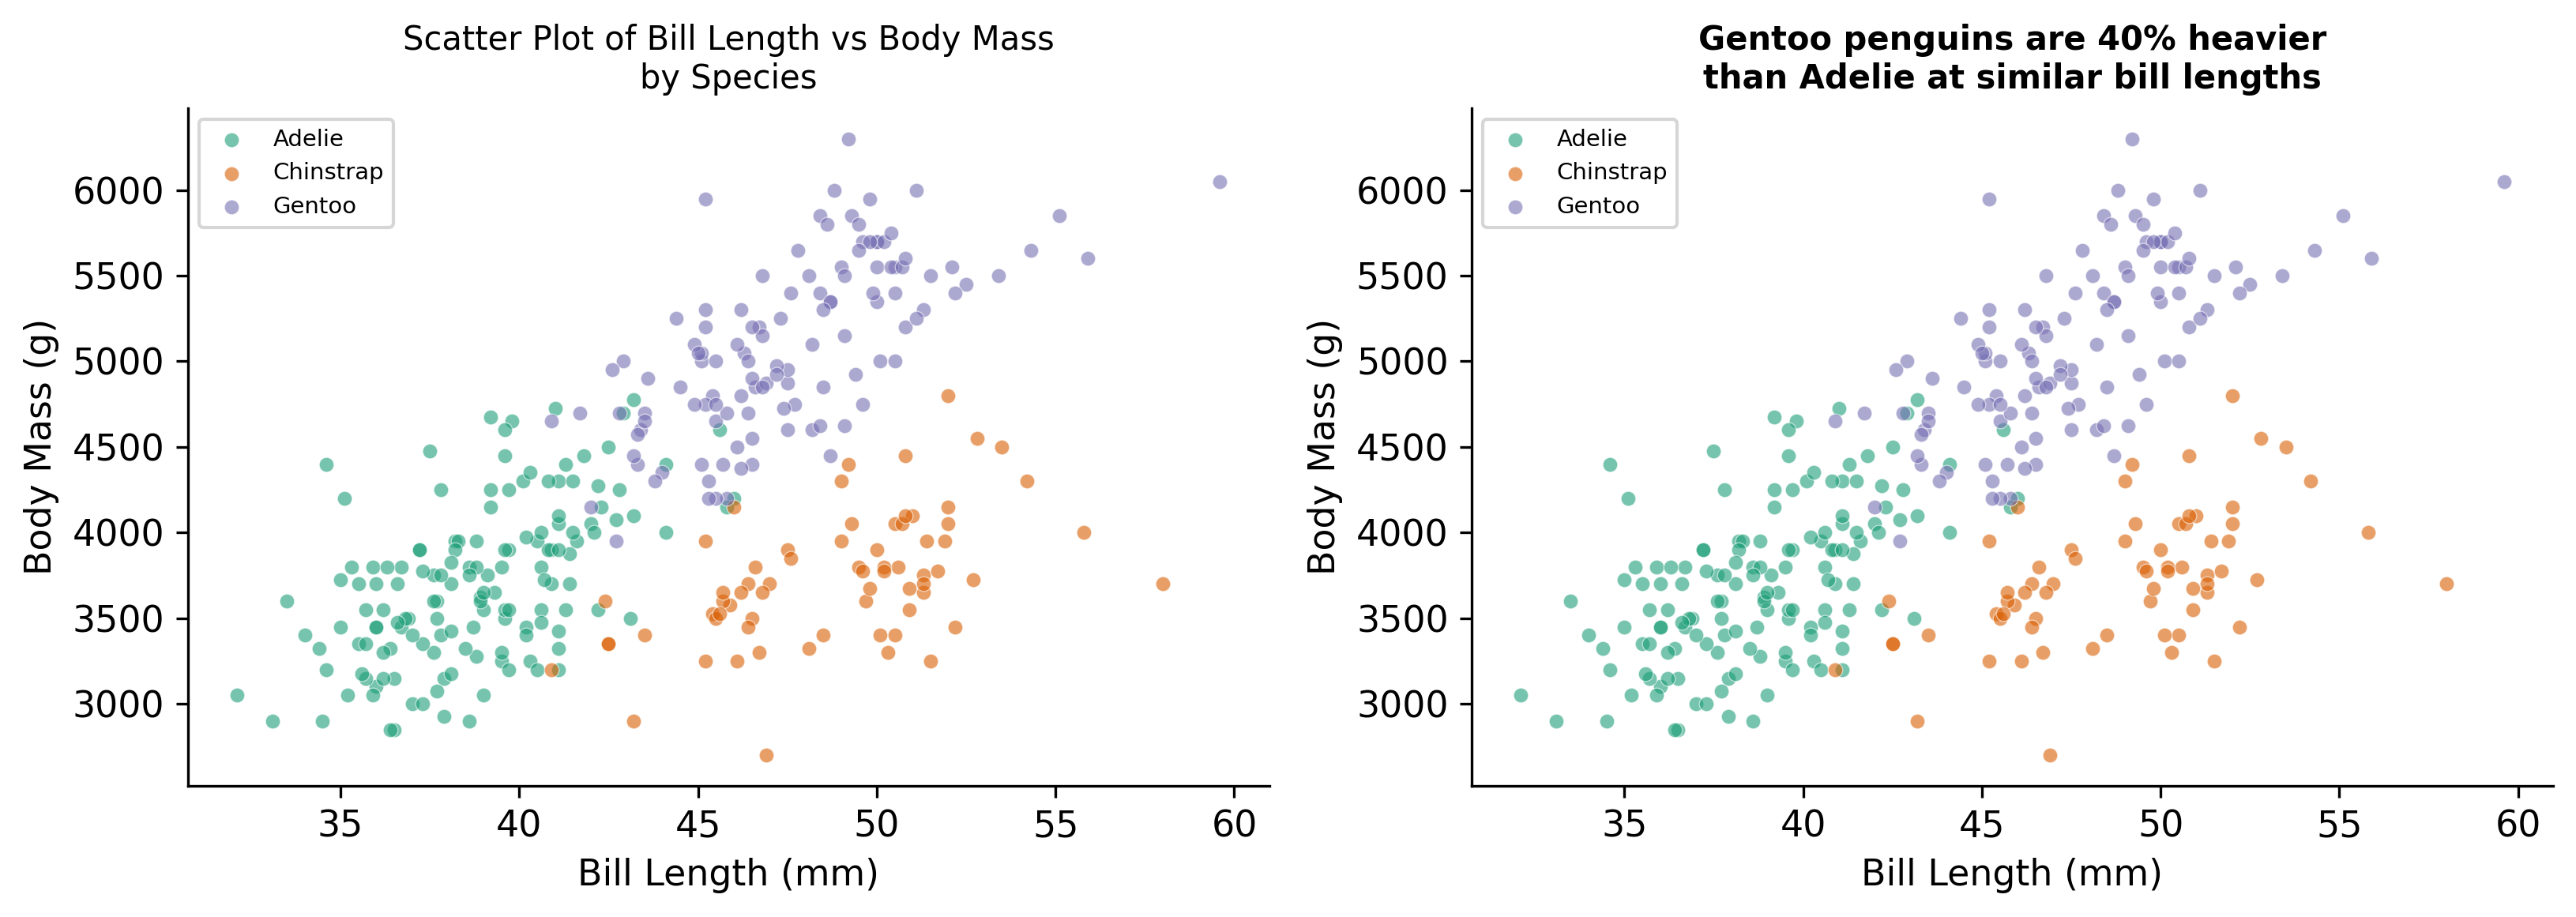
\includegraphics[width=0.88\textwidth]{m1_9_title_claim.png}

\vspace{0.2cm}
\begin{columns}[T]
\begin{column}{0.48\textwidth}
\begin{exampleblock}{Data Insight}
    \scriptsize Left: descriptive title (``Scatter Plot of\ldots'') tells the reader nothing they can't already see. Right: analytical title states the \textbf{conclusion} --- the reader knows what to look for before scanning the data.
\end{exampleblock}
\end{column}
\begin{column}{0.48\textwidth}
\begin{alertblock}{Pro-Tip}
    \scriptsize Formula: Title = \textbf{who/what} + \textbf{does what} + \textbf{by how much}. ``Gentoo penguins are 40\% heavier than Adelie at similar bill lengths.''
\end{alertblock}
\end{column}
\end{columns}
\end{frame}

% ── 255 ──
\begin{frame}{Subtitles, Captions, and Source Attribution}
\smark{255/300}
\centering
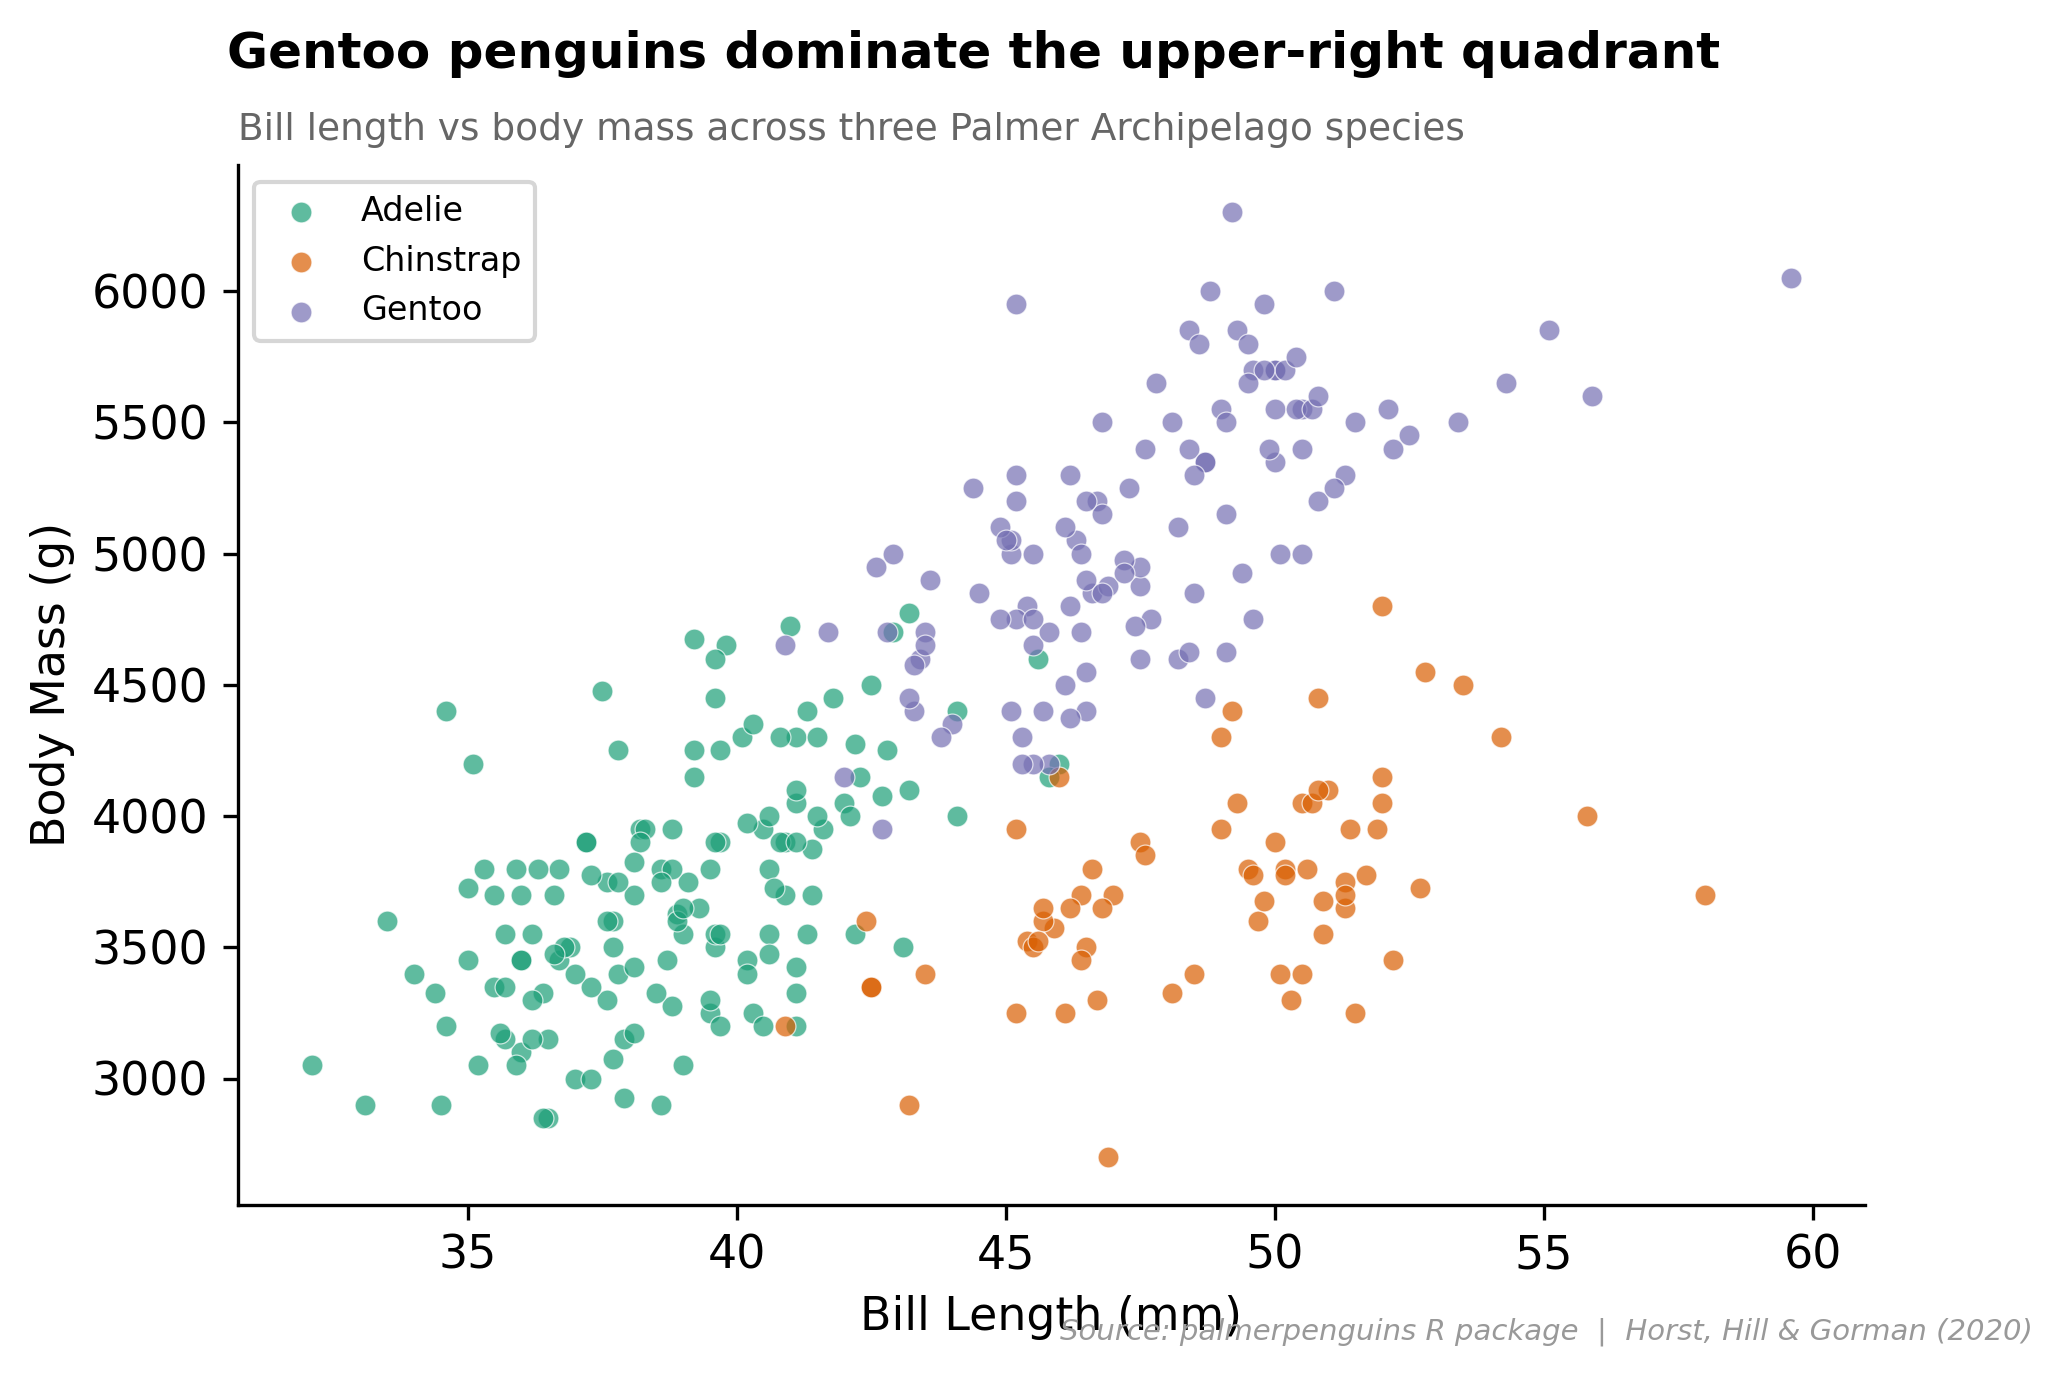
\includegraphics[width=0.72\textwidth]{m1_9_subtitle_caption.png}

\vspace{0.2cm}
\begin{columns}[T]
\begin{column}{0.48\textwidth}
\begin{itemize}
    \item \textbf{Title}: the analytical claim (bold, large)
    \item \textbf{Subtitle}: methodological context (smaller, grey)
    \item \textbf{Caption}: data source, date, author (bottom-right, italics)
\end{itemize}
\end{column}
\begin{column}{0.48\textwidth}
\begin{alertblock}{Pro-Tip}
    \scriptsize In ggplot2: \texttt{labs(title=, subtitle=, caption=)}. All three are positioned automatically. In matplotlib: use \texttt{fig.suptitle()}, \texttt{ax.set\_title()}, and \texttt{fig.text()} for the caption.
\end{alertblock}
\end{column}
\end{columns}
\end{frame}

% ── 256 ──
\begin{frame}[fragile]{Title + Subtitle + Caption --- Code}\smark{256/300}
\begin{columns}[T]
\begin{column}{0.48\textwidth}
\begin{lstlisting}[style=Rstyle]
ggplot(penguins, aes(...)) +
  geom_point() +
  labs(
    title = "Gentoo dominate
      the upper-right",
    subtitle = "Bill length vs
      body mass, 3 species",
    caption = "Source:
      palmerpenguins (2020)",
    x = "Bill Length (mm)",
    y = "Body Mass (g)") +
  theme(
    plot.title = element_text(
      face="bold", size=13),
    plot.subtitle = element_text(
      color="#666", size=10),
    plot.caption = element_text(
      face="italic",
      color="#999", size=8))
\end{lstlisting}
\end{column}
\begin{column}{0.48\textwidth}
\begin{lstlisting}[style=Pystyle]
# matplotlib
fig.suptitle(
    "Gentoo dominate the "
    "upper-right",
    fontweight="bold",
    fontsize=12, x=0.12,
    ha="left")
ax.set_title(
    "Bill length vs body mass",
    fontsize=9, color="#666",
    loc="left")
fig.text(0.98, 0.01,
    "Source: palmerpenguins",
    fontsize=7, color="#999",
    ha="right", style="italic")
\end{lstlisting}
\end{column}
\end{columns}
\end{frame}

% ── 257 ──
\begin{frame}{\texttt{geom\_text} and \texttt{geom\_label}}
\smark{257/300}
\begin{columns}[T]
\begin{column}{0.50\textwidth}
\begin{itemize}
    \item \texttt{geom\_text()}: bare text at data coordinates
    \item \texttt{geom\_label()}: text with a filled rectangle behind it (more visible, more ink)
    \item Both map \texttt{aes(label = column)} from data
    \item Common use: bar chart value labels, map city names, scatter point IDs
\end{itemize}
\end{column}
\begin{column}{0.47\textwidth}
\begin{alertblock}{Pro-Tip}
    \scriptsize \texttt{geom\_text()} is data-driven (one label per row). \texttt{annotate("text")} is manual (one fixed label). Don't confuse them --- using \texttt{geom\_text()} with manual coordinates creates $n$ copies.
\end{alertblock}
\vspace{0.2cm}
\begin{exampleblock}{Data Insight}
    \scriptsize Add \texttt{vjust=-1} to push text above points. Add \texttt{check\_overlap=TRUE} for a quick-and-dirty overlap fix (drops labels that collide).
\end{exampleblock}
\end{column}
\end{columns}
\end{frame}

% ── 258 ──
\begin{frame}[fragile]{\texttt{geom\_text} / \texttt{geom\_label} --- Code}\smark{258/300}
\begin{columns}[T]
\begin{column}{0.48\textwidth}
\begin{lstlisting}[style=Rstyle]
# Text labels on bar chart
ggplot(df, aes(region, sales)) +
  geom_col(fill="#2166AC") +
  geom_text(aes(label=sales),
    vjust = -0.5, size = 3.5)

# Label (with background)
ggplot(df, aes(x, y)) +
  geom_point() +
  geom_label(aes(label=name),
    size = 2.5, alpha = 0.8,
    label.padding = unit(0.15,
      "lines"))
\end{lstlisting}
\end{column}
\begin{column}{0.48\textwidth}
\begin{lstlisting}[style=Pystyle]
# matplotlib: bar value labels
for i, v in enumerate(vals):
    ax.text(i, v+0.5, str(v),
            ha="center", fontsize=9)

# plotnine
(ggplot(df, aes("x","y"))
 + geom_point()
 + geom_text(aes(label="name"),
     size=8, nudge_y=0.3))

# geom_label in plotnine
(ggplot(df, aes("x","y"))
 + geom_label(aes(label="name"),
     size=7, alpha=0.8))
\end{lstlisting}
\end{column}
\end{columns}
\end{frame}

% ── 259 ──
\begin{frame}{\texttt{ggrepel} / \texttt{adjustText}: Non-Overlapping Labels}
\smark{259/300}
\centering
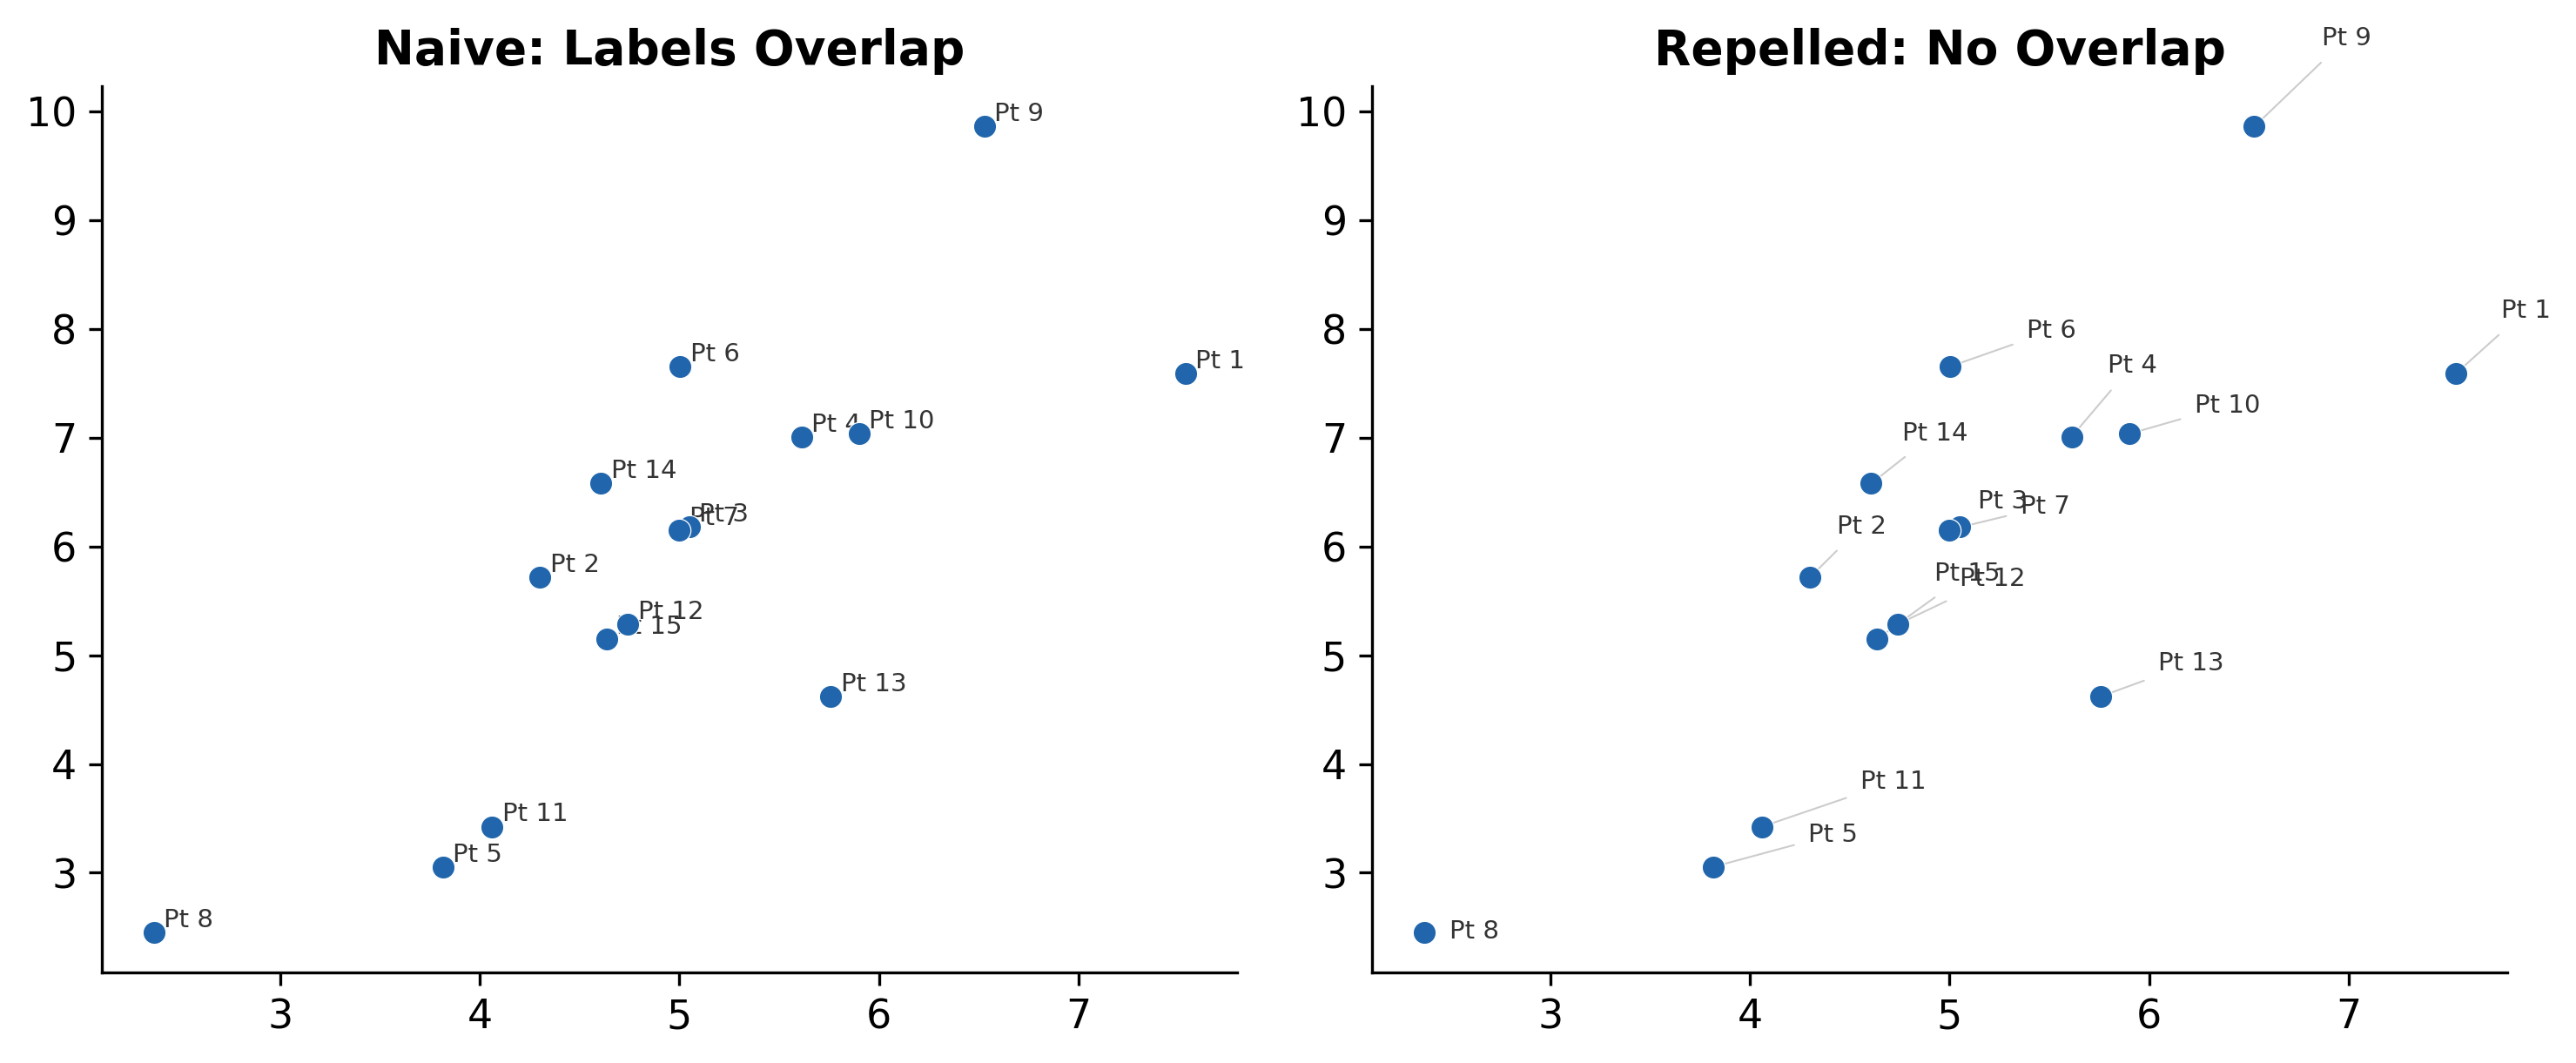
\includegraphics[width=0.85\textwidth]{m1_9_text_repel.png}

\vspace{0.2cm}
\begin{columns}[T]
\begin{column}{0.48\textwidth}
\begin{exampleblock}{Data Insight}
    \scriptsize Left: naive \texttt{geom\_text()} places labels at data coordinates --- dense regions become unreadable. Right: \texttt{ggrepel} iteratively pushes labels apart and draws leader lines.
\end{exampleblock}
\end{column}
\begin{column}{0.48\textwidth}
\begin{alertblock}{Pro-Tip}
    \scriptsize For $>$30 labels, even repelling fails. Label only the top/bottom $k$ points, or use interactive tooltips (Module 8).
\end{alertblock}
\end{column}
\end{columns}
\end{frame}

% ── 260 ──
\begin{frame}[fragile]{\texttt{ggrepel} / \texttt{adjustText} --- Code}\smark{260/300}
\begin{columns}[T]
\begin{column}{0.48\textwidth}
\begin{lstlisting}[style=Rstyle]
library(ggrepel)

ggplot(top_points,
  aes(x, y, label=name)) +
  geom_point(color="#2166AC") +
  geom_text_repel(
    size = 3,
    max.overlaps = 15,
    segment.color = "#CCCCCC",
    segment.size = 0.3) +
  theme_minimal()

# geom_label_repel for boxes
\end{lstlisting}
\end{column}
\begin{column}{0.48\textwidth}
\begin{lstlisting}[style=Pystyle]
# pip install adjustText
from adjustText import adjust_text

texts = []
for i, row in top.iterrows():
    texts.append(
        ax.text(row.x, row.y,
                row["name"],
                fontsize=8))

adjust_text(texts,
    arrowprops=dict(
        arrowstyle="-",
        color="#CCC", lw=0.5))
\end{lstlisting}
\vspace{0.1cm}
\begin{exampleblock}{Data Insight}
    \scriptsize \texttt{adjust\_text()} is the \texttt{ggrepel} equivalent. Pass a list of \texttt{ax.text()} objects; it repositions them iteratively.
\end{exampleblock}
\end{column}
\end{columns}
\end{frame}

% ── 261 ──
\begin{frame}{Annotation in Faceted Plots}
\smark{261/300}
\begin{columns}[T]
\begin{column}{0.50\textwidth}
\begin{itemize}
    \item \texttt{annotate()} draws in \textbf{every} panel (no facet variable)
    \item \texttt{geom\_text(data=...)} with the facet variable draws in the \textbf{matching} panel only
    \item To annotate one specific panel: create a 1-row data frame with the facet column set
\end{itemize}
\end{column}
\begin{column}{0.47\textwidth}
\begin{alertblock}{Pro-Tip}
    \scriptsize To add ``n = 146'' to just the Adelie panel: \texttt{geom\_text(data = tibble(species="Adelie", x=55, y=5800, label="n=146"), aes(x, y, label=label))}. The facet variable in the data frame routes it to the correct panel.
\end{alertblock}
\end{column}
\end{columns}
\end{frame}

% ── 262 ──
\begin{frame}[fragile]{Facet-Specific Annotations --- Code}\smark{262/300}
\begin{columns}[T]
\begin{column}{0.48\textwidth}
\begin{lstlisting}[style=Rstyle]
# Annotation in ALL panels
ggplot(...) +
  facet_wrap(~species) +
  annotate("text", x=55, y=6000,
    label="Global note")

# Annotation in ONE panel
label_df <- tibble(
  species = "Gentoo",
  x = 55, y = 6000,
  label = "n = 119")
ggplot(...) +
  facet_wrap(~species) +
  geom_text(data = label_df,
    aes(x, y, label=label),
    fontface="bold", size=3)
\end{lstlisting}
\end{column}
\begin{column}{0.48\textwidth}
\begin{lstlisting}[style=Pystyle]
# plotnine: same approach
label_df = pd.DataFrame({
    "species": ["Gentoo"],
    "x": [55], "y": [6000],
    "label": ["n = 119"]})

(ggplot(...) +
 facet_wrap("~species") +
 geom_text(data=label_df,
    mapping=aes("x","y",
                label="label"),
    fontweight="bold", size=9))
\end{lstlisting}
\end{column}
\end{columns}
\end{frame}

% ── 263 ──
\begin{frame}{Storytelling: Guiding the Reader's Eye}
\smark{263/300}
\begin{columns}[T]
\begin{column}{0.50\textwidth}
    \textbf{The visual hierarchy:}
    \begin{itemize}
        \item \textbf{Title}: states the insight (read first)
        \item \textbf{Highlighted data}: saturated color, large
        \item \textbf{Context data}: grey, small, background
        \item \textbf{Annotation}: arrow + label at the key point
        \item \textbf{Caption}: source and method (read last)
    \end{itemize}
\end{column}
\begin{column}{0.47\textwidth}
\begin{exampleblock}{Data Insight}
    \scriptsize The reader's eye follows a Z-pattern: title (top-left) $\to$ highlighted data (center) $\to$ annotation (where the arrow points) $\to$ caption (bottom-right). Design your layers to match this flow.
\end{exampleblock}
\end{column}
\end{columns}
\end{frame}

% ── 264 ──
\begin{frame}{The ``Explanatory Figure'' Template}
\smark{264/300}
\begin{columns}[T]
\begin{column}{0.50\textwidth}
    \textbf{Layer stack (bottom to top):}
    \begin{enumerate}
        \item Grey context (all data, low alpha)
        \item Colored target group (saturated)
        \item Trend line or smoother
        \item Reference lines (threshold, mean)
        \item Text annotation (insight callout)
        \item Title as claim + subtitle + caption
    \end{enumerate}
\end{column}
\begin{column}{0.47\textwidth}
\begin{alertblock}{Pro-Tip}
    \scriptsize This is the structure used by FiveThirtyEight, The Economist, and NYT graphics desks. Data first, then progressively more interpretive layers on top.
\end{alertblock}
\vspace{0.2cm}
\begin{exampleblock}{Data Insight}
    \scriptsize Each layer adds \textbf{one unit of meaning}. If you remove a layer and the reader loses understanding, it earned its ink. If not, delete it.
\end{exampleblock}
\end{column}
\end{columns}
\end{frame}

% ── 265 ──
\begin{frame}[fragile]{Explanatory Figure --- \Rlang}\smark{265/300}
\begin{columns}[T]
\begin{column}{0.55\textwidth}
\begin{lstlisting}[style=Rstyle]
ggplot(penguins, aes(
    bill_length_mm, body_mass_g))+
  # 1. Grey context
  geom_point(color="#DDD",
    size=1, alpha=0.3) +
  # 2. Target group
  geom_point(
    data=filter(penguins,
      species=="Gentoo"),
    color="#7570B3", alpha=0.8) +
  # 3. Trend line
  geom_smooth(
    data=filter(penguins,
      species=="Gentoo"),
    method="lm", se=FALSE,
    color="#7570B3") +
  # 4. Mean reference
  geom_hline(yintercept=5076,
    linetype="dashed",
    color="#B2182B") +
  # 5+6. Labels
  labs(title="Gentoo are the
    heaviest species",
    caption="Source: Palmer")
\end{lstlisting}
\end{column}
\begin{column}{0.42\textwidth}
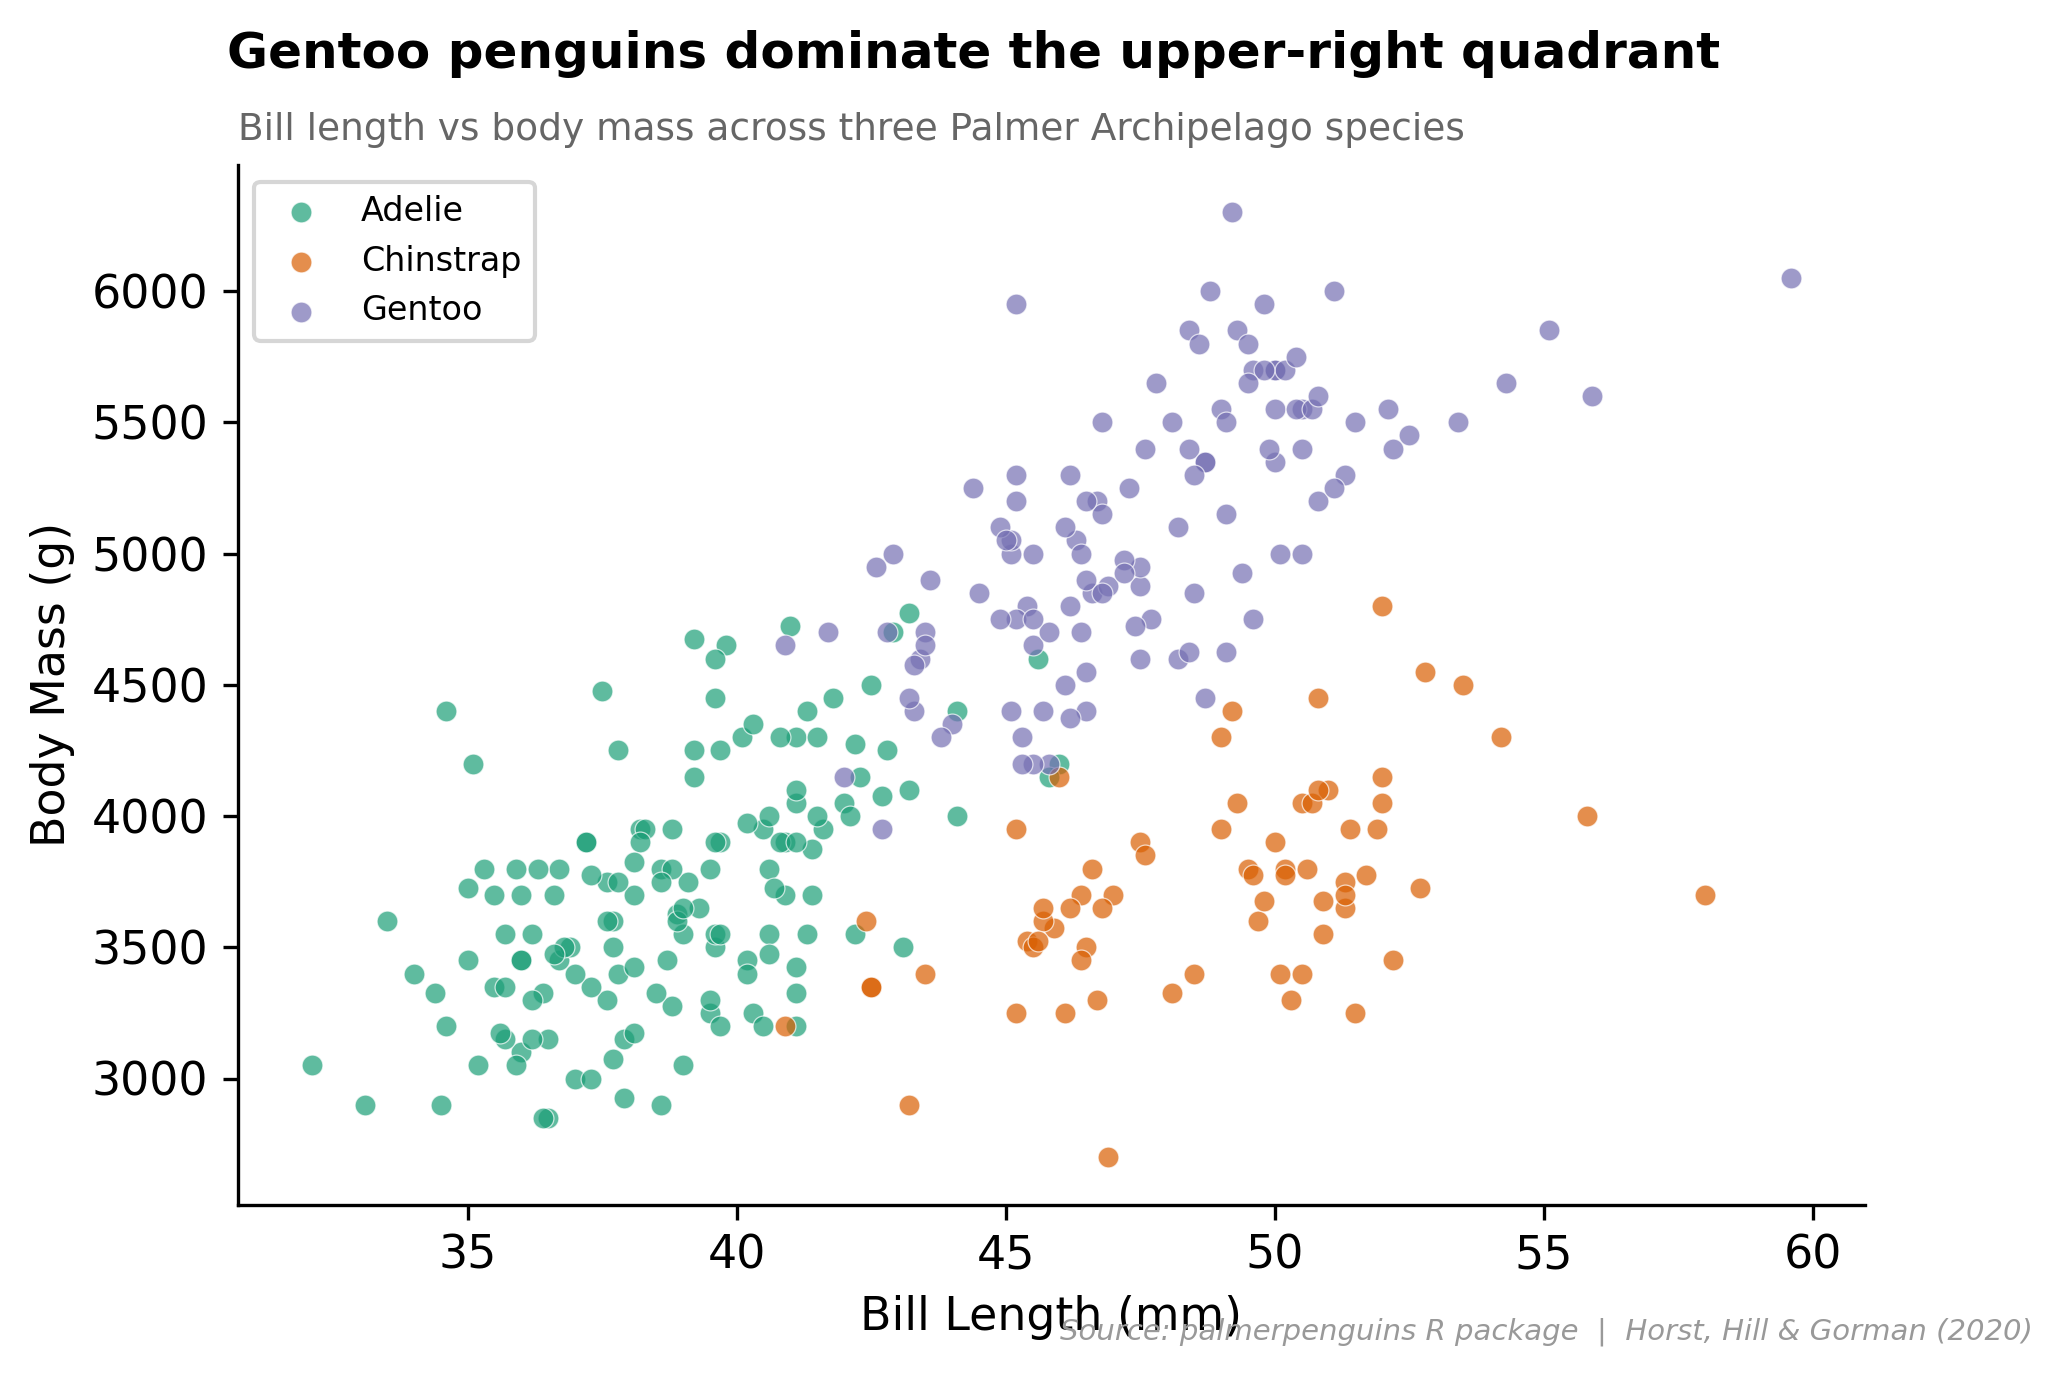
\includegraphics[width=\textwidth]{m1_9_subtitle_caption.png}
\begin{exampleblock}{Data Insight}
    \scriptsize Six layers, each adding one semantic unit. Remove any one and the figure loses information. This is the data-ink test applied to annotation.
\end{exampleblock}
\end{column}
\end{columns}
\end{frame}

% ── 266 ──
\begin{frame}[fragile]{Explanatory Figure --- \Python}\smark{266/300}
\begin{columns}[T]
\begin{column}{0.55\textwidth}
\begin{lstlisting}[style=Pystyle]
fig, ax = plt.subplots()
# 1. Grey context
ax.scatter(pen.bill_length_mm,
    pen.body_mass_g,
    color="#DDD", s=8, alpha=0.3)
# 2. Target
g = pen[pen.species=="Gentoo"]
ax.scatter(g.bill_length_mm,
    g.body_mass_g,
    color="#7570B3", alpha=0.8)
# 3. Trend
z = np.polyfit(g.bill_length_mm,
    g.body_mass_g, 1)
ax.plot(xfit, np.polyval(z, xfit),
    color="#7570B3")
# 4. Reference
ax.axhline(y=5076, linestyle="--",
    color="#B2182B")
# 5+6. Labels
fig.suptitle("Gentoo are heaviest",
    fontweight="bold")
fig.text(0.98, 0.01,
    "Source: Palmer",
    fontsize=7, ha="right")
\end{lstlisting}
\end{column}
\begin{column}{0.42\textwidth}
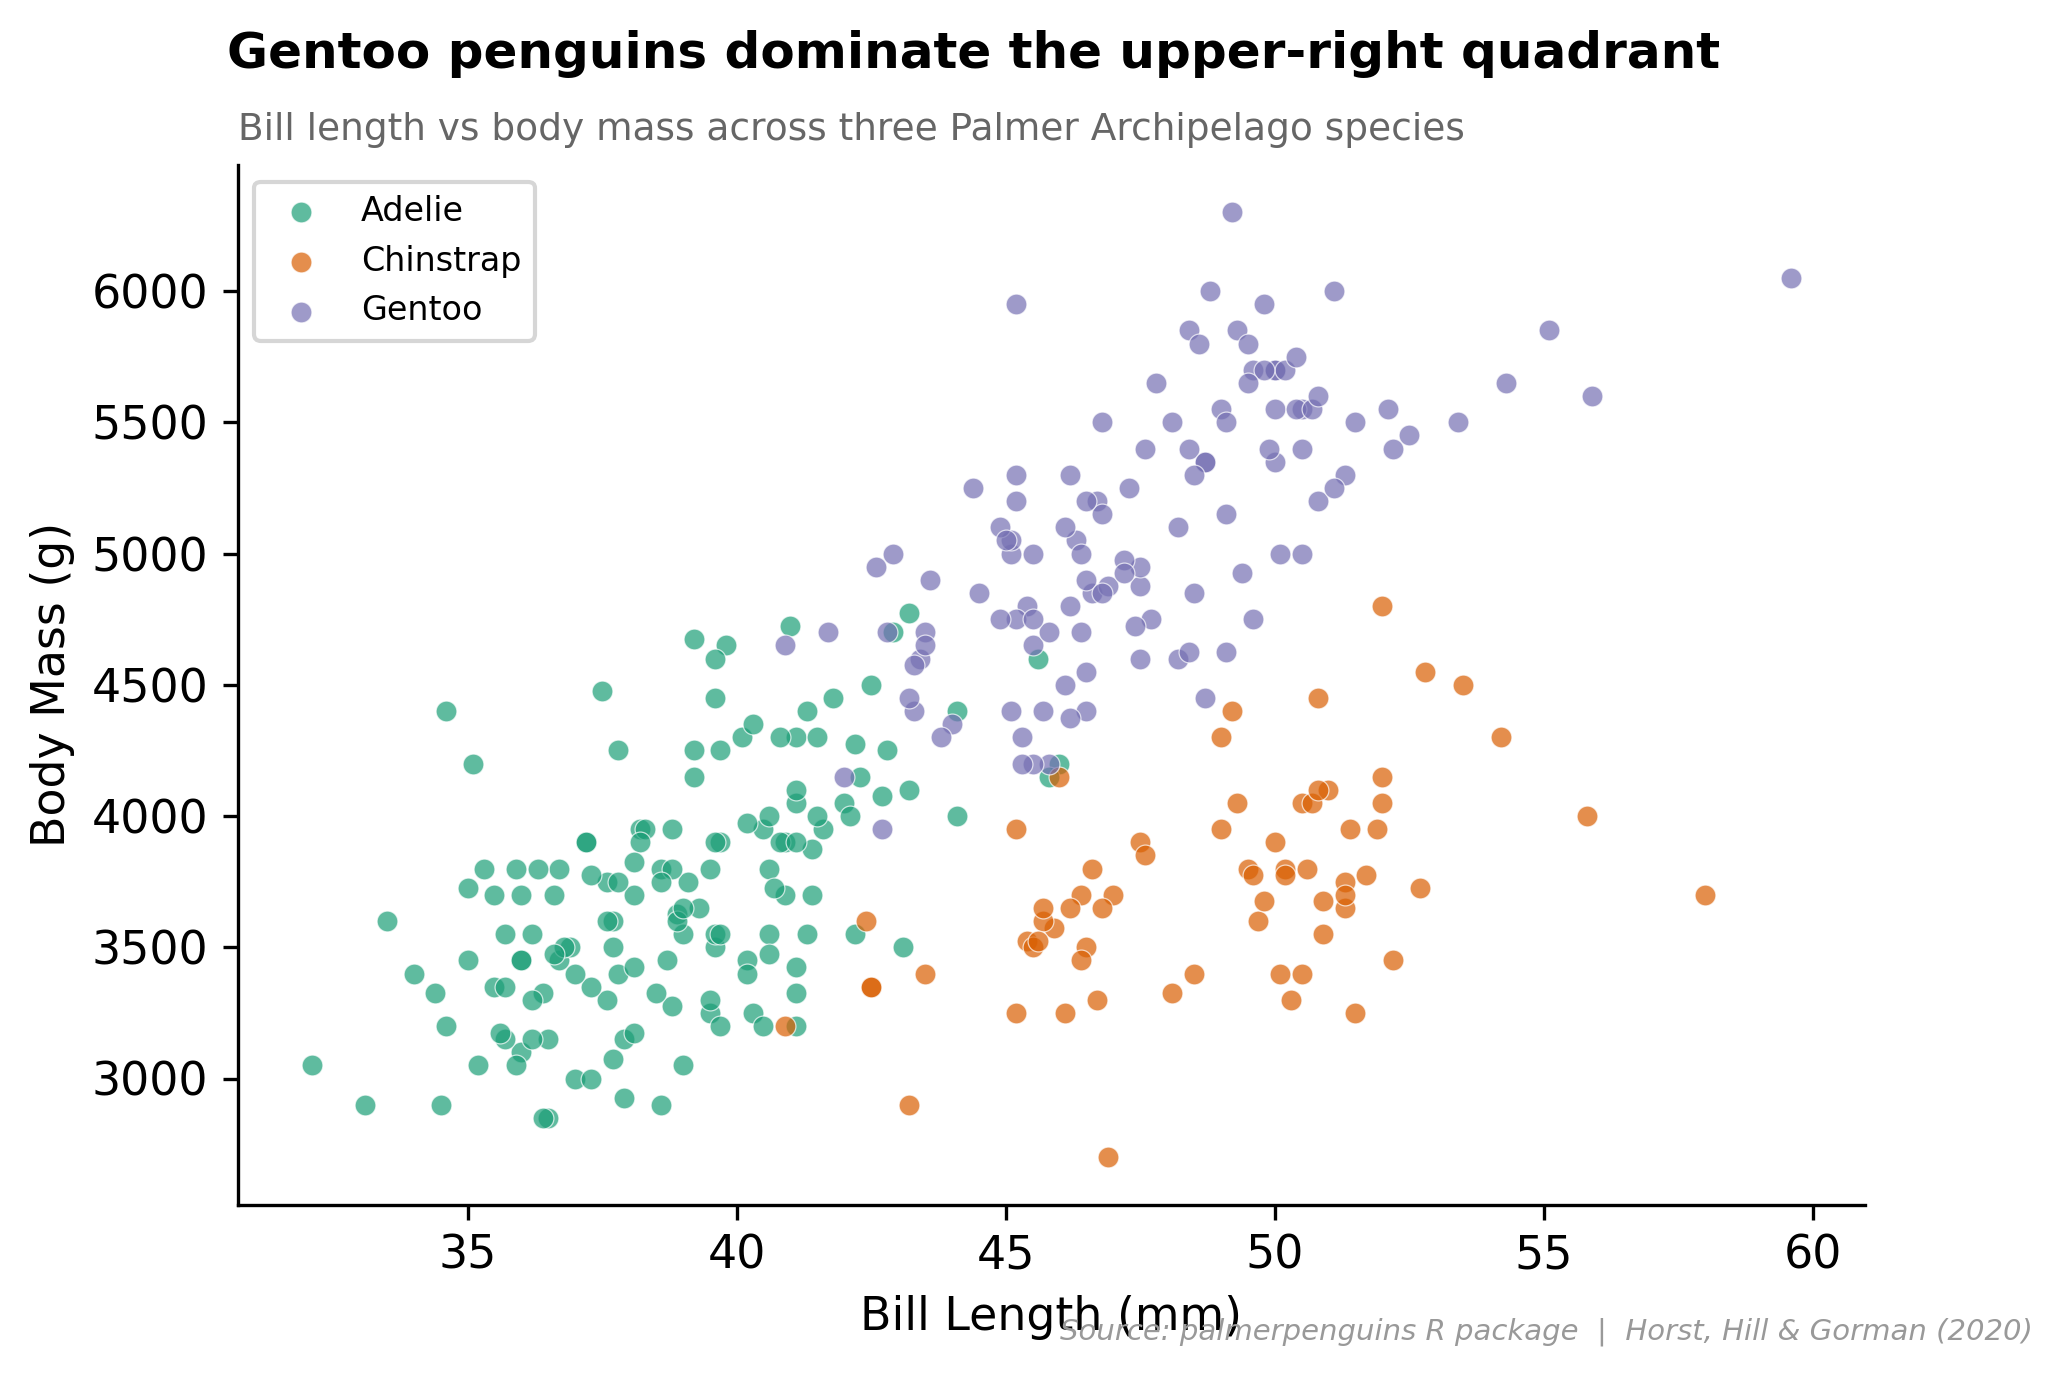
\includegraphics[width=\textwidth]{m1_9_subtitle_caption.png}
\end{column}
\end{columns}
\end{frame}

% ── 267 ──
\begin{frame}{Common Annotation Mistakes}
\smark{267/300}
\centering\small
\begin{tabular}{@{}ll@{}}
    \toprule
    \textbf{Mistake} & \textbf{Fix} \\
    \midrule
    Arrow points to empty space           & Anchor \texttt{xy=} at the data point \\
    Label overlaps data                   & Use \texttt{ggrepel} / \texttt{adjustText} \\
    Annotation in wrong facet panel       & Include facet variable in annotation data \\
    Title describes the chart type        & Title states the \textbf{insight} \\
    Too many annotations                  & 1--3 per plot; annotate the \emph{message} \\
    Reference line without label          & Add \texttt{annotate("text")} next to the line \\
    Caption missing source                & Always attribute data origin \\
    \bottomrule
\end{tabular}

\vspace{0.3cm}
\begin{alertblock}{Pro-Tip}
    \scriptsize The most common mistake: an unlabeled reference line. A dashed line at $y=4200$ means nothing without ``Mean = 4200 g'' next to it.
\end{alertblock}
\end{frame}

% ── 268 ──
\begin{frame}{Annotation Decision Flowchart}
\smark{268/300}
\centering\small
\begin{tabular}{@{}lll@{}}
    \toprule
    \textbf{Goal} & \textbf{Tool} & \textbf{Package} \\
    \midrule
    Label 1--3 specific points  & \texttt{annotate("text")} + arrow & base ggplot2 \\
    Label every point           & \texttt{geom\_text(aes(label=))}  & base ggplot2 \\
    Non-overlapping labels      & \texttt{geom\_text\_repel()}      & \texttt{ggrepel} \\
    Horizontal threshold        & \texttt{geom\_hline()}            & base ggplot2 \\
    Event period shading        & \texttt{annotate("rect")}         & base ggplot2 \\
    Title as claim              & \texttt{labs(title=)}              & base ggplot2 \\
    Source attribution           & \texttt{labs(caption=)}           & base ggplot2 \\
    \bottomrule
\end{tabular}
\end{frame}

% ── 269 ──
\begin{frame}{Module 1.9 --- Key Takeaways}\smark{269/300}
\begin{enumerate}
    \item \textbf{Title = insight.} Not ``Scatter of X vs Y'' but ``X causes 40\% increase in Y.''
    \item \textbf{Direct labels $>$ legends} when groups $\leq$5.
    \item \textbf{Reference lines need labels.} A dashed line without text is meaningless.
    \item \textbf{Shaded regions} for event windows and confidence bands.
    \item \textbf{\texttt{ggrepel} / \texttt{adjustText}} for non-overlapping text.
    \item \textbf{1--3 annotations per plot.} Each earns its ink or gets cut.
\end{enumerate}
\end{frame}

% ── 270 ──
\begin{frame}{}\smark{270/300}
\centering\vspace{1.5cm}
{\Large\textbf{Module 1.9 Complete}}\\[0.5cm]
You can now annotate any plot with text, arrows, reference lines, shaded regions, direct labels, and analytical titles --- transforming exploratory charts into explanatory figures.\\[0.5cm]
\textbf{Next:} Module 1.10 --- Exporting, Reproducibility, and Workflow.
\end{frame}

% ═══════════════════════════════════════════════════════
%  MODULE 1.10 — Exporting, Reproducibility, and Workflow
% ═══════════════════════════════════════════════════════
\section{Module 1.10 --- Exporting, Reproducibility, and Workflow}

% ── 271 ──
\begin{frame}{Module 1.10 --- Roadmap}\smark{271/300}
\begin{enumerate}
    \item Vector vs.\ raster output formats
    \item DPI and resolution for print vs.\ screen
    \item \texttt{ggsave()} and \texttt{plt.savefig()} parameters
    \item Figure sizing: single-column, double-column, slide
    \item Reproducible project structure
    \item R Markdown / Quarto figure chunks
    \item Jupyter notebook figure management
    \item Version control for figures
\end{enumerate}
\end{frame}

% ── 272 ──
\begin{frame}{The Figure Workflow}
\smark{272/300}
\centering
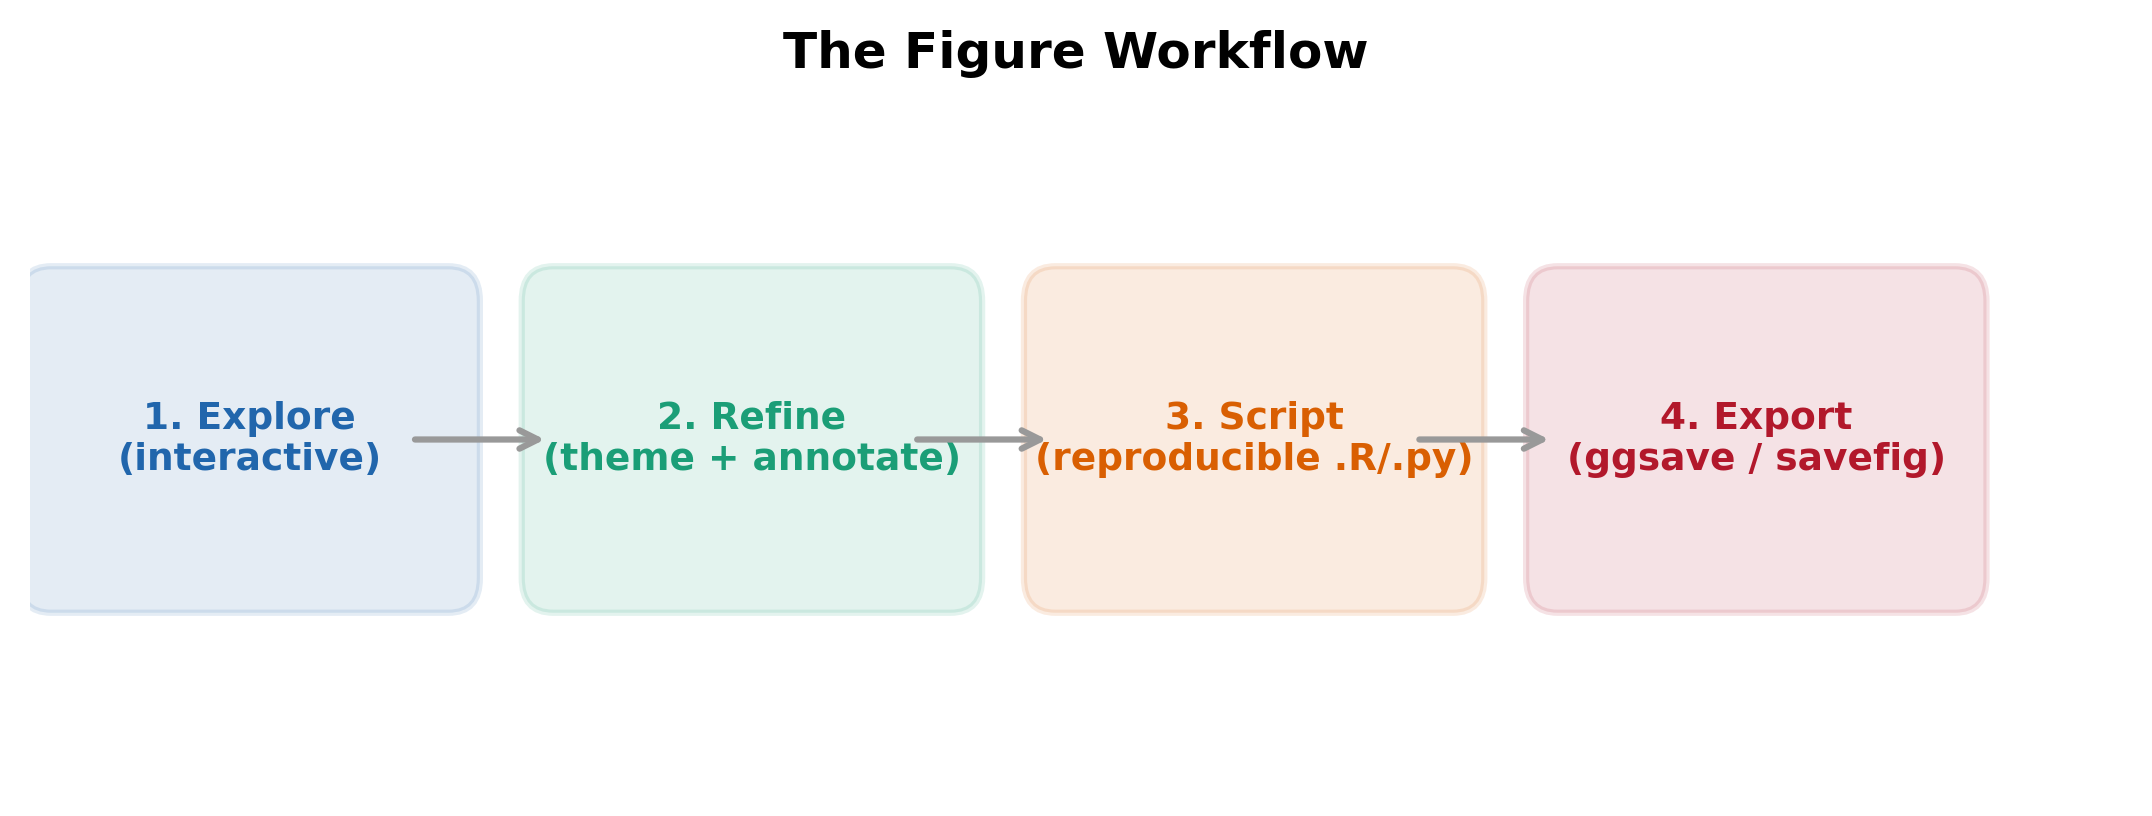
\includegraphics[width=0.88\textwidth]{m1_10_workflow.png}

\vspace{0.3cm}
\begin{exampleblock}{Data Insight}
    \scriptsize Every publication-quality figure passes through four stages: interactive exploration, theme and annotation refinement, scripting for reproducibility, and export with controlled dimensions and resolution.
\end{exampleblock}
\end{frame}

% ── 273 ──
\begin{frame}{Vector vs.\ Raster: Choosing Your Format}
\smark{273/300}
\centering
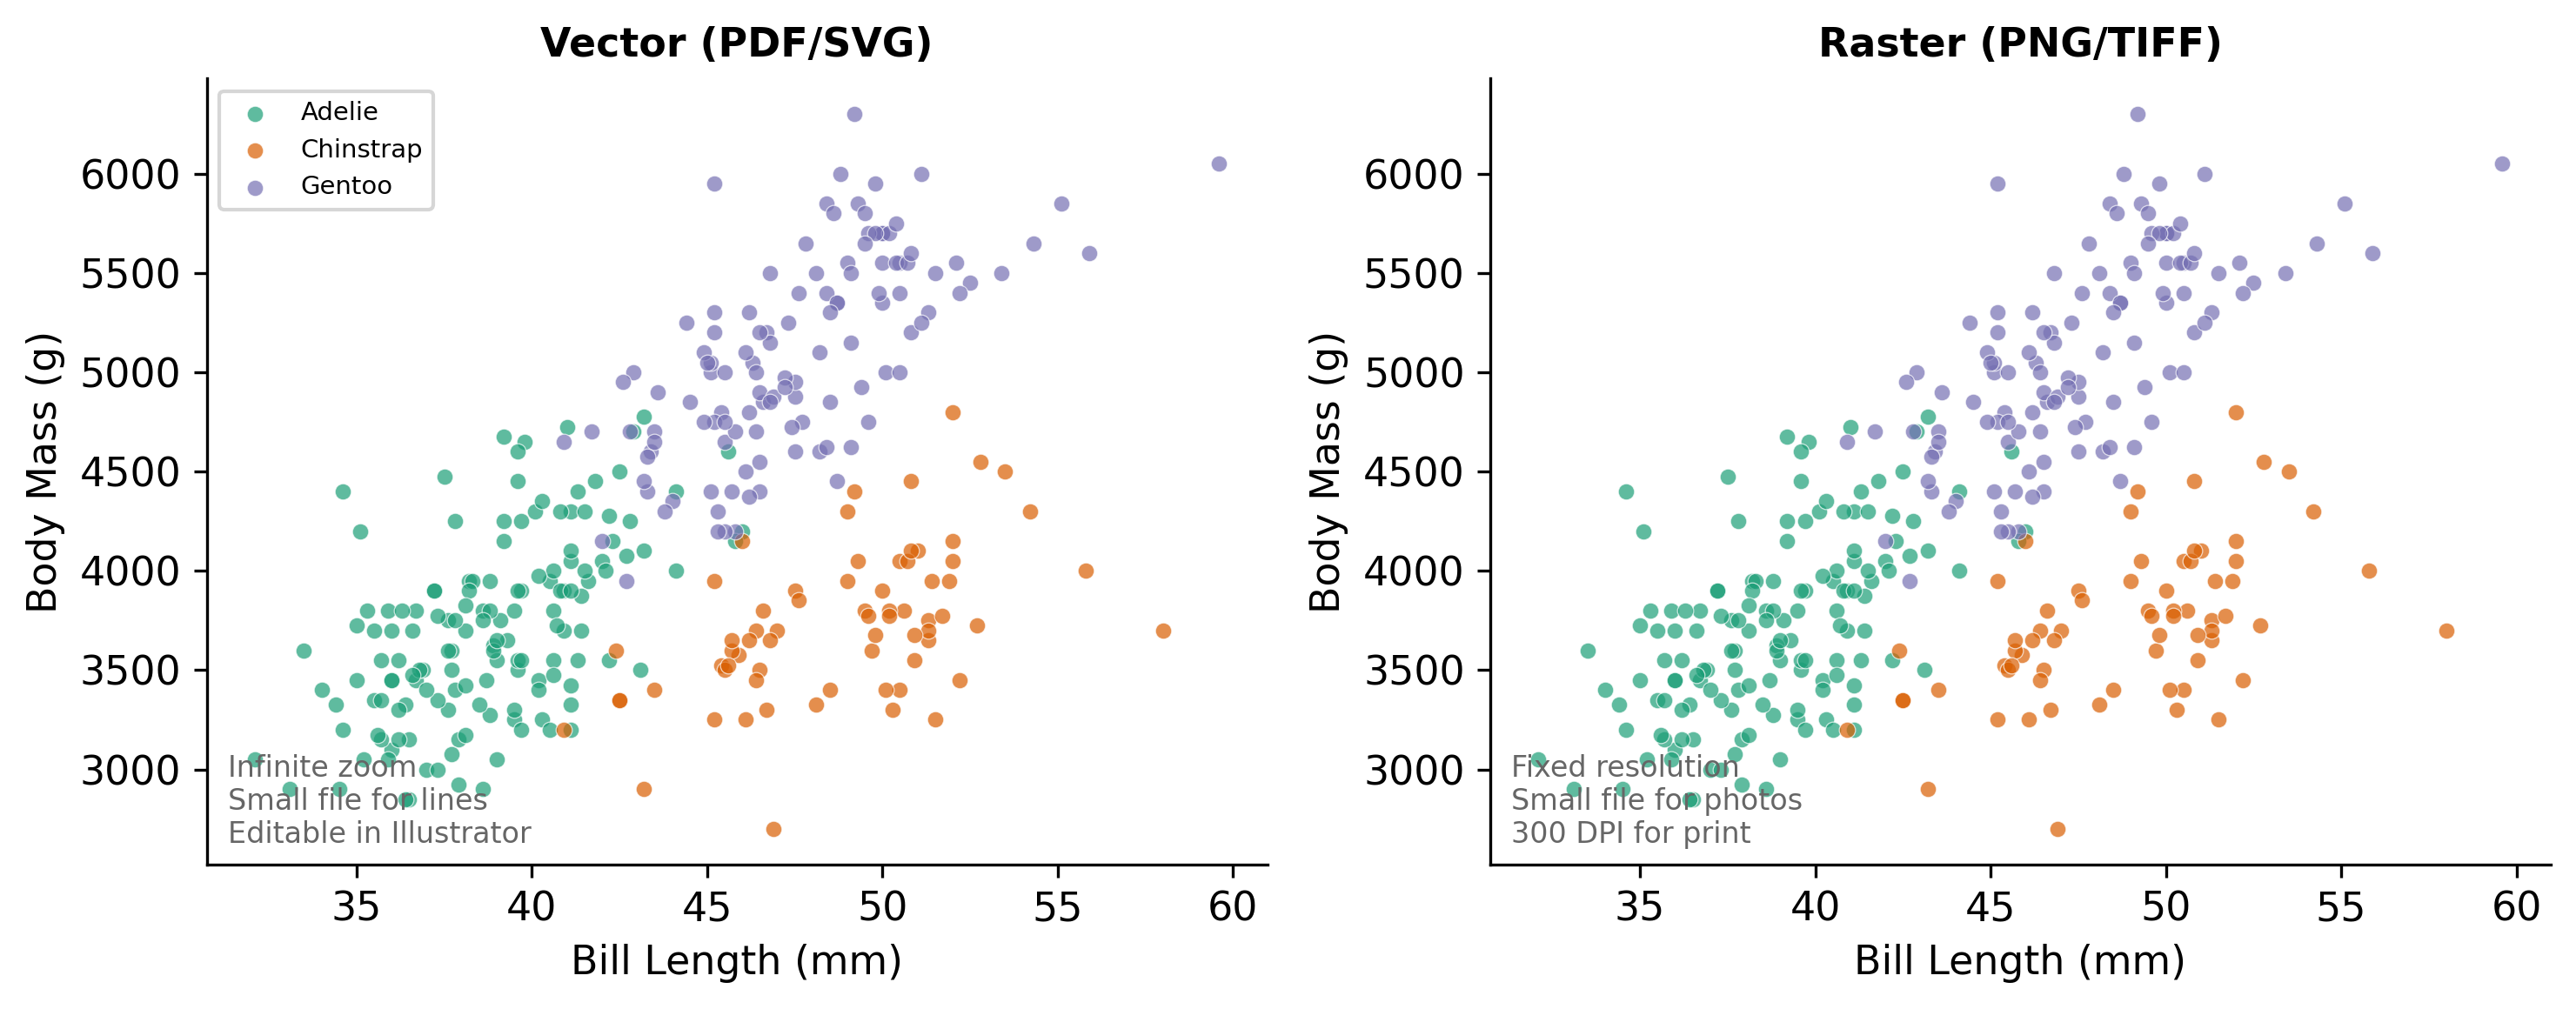
\includegraphics[width=0.85\textwidth]{m1_10_vector_raster.png}

\vspace{0.2cm}
\centering\small
\begin{tabular}{@{}lll@{}}
    \toprule
    \textbf{Property} & \textbf{Vector (PDF, SVG, EPS)} & \textbf{Raster (PNG, TIFF, JPEG)} \\
    \midrule
    Zoom        & Infinite, no pixelation  & Degrades at high zoom \\
    File size   & Small for lines/points   & Small for photos/heatmaps \\
    Editing     & Illustrator / Inkscape   & Photoshop / GIMP \\
    Use case    & Journals, presentations  & Web, complex heatmaps \\
    \bottomrule
\end{tabular}
\end{frame}

% ── 274 ──
\begin{frame}{DPI: Resolution for Print and Screen}
\smark{274/300}
\centering
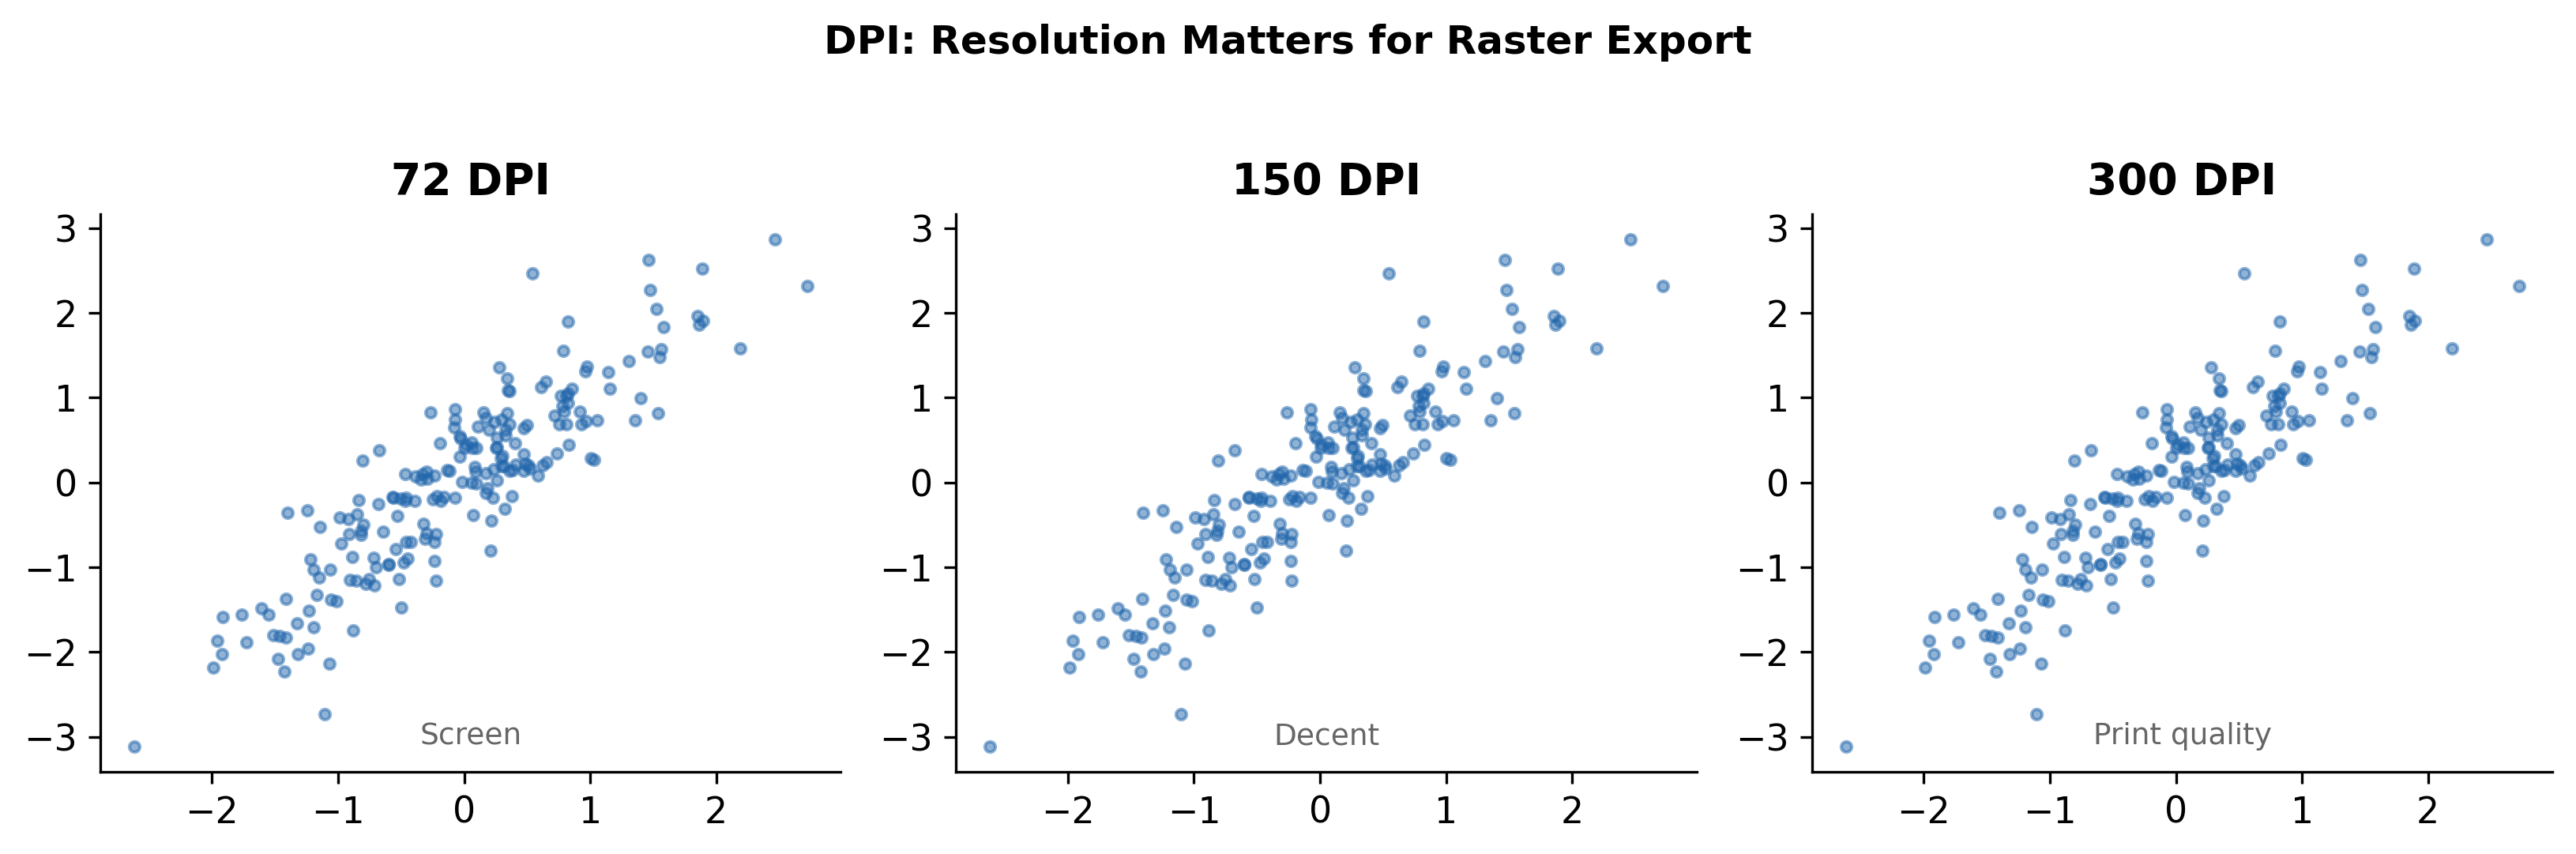
\includegraphics[width=0.85\textwidth]{m1_10_dpi.png}

\vspace{0.2cm}
\begin{columns}[T]
\begin{column}{0.48\textwidth}
\centering\small
\begin{tabular}{@{}lr@{}}
    \toprule
    \textbf{Context} & \textbf{DPI} \\
    \midrule
    Web / screen       & 72--96 \\
    Slide presentations & 150 \\
    Journal (minimum)   & 300 \\
    Line art (journal)  & 600 \\
    \bottomrule
\end{tabular}
\end{column}
\begin{column}{0.48\textwidth}
\begin{alertblock}{Pro-Tip}
    \scriptsize DPI only matters for \textbf{raster} formats. Vector outputs (PDF, SVG) are resolution-independent. Export PDF for the journal and PNG at 300 DPI for the supplementary website.
\end{alertblock}
\end{column}
\end{columns}
\end{frame}

% ── 275 ──
\begin{frame}{\texttt{ggsave()} / \texttt{savefig()} Parameters}
\smark{275/300}
\centering
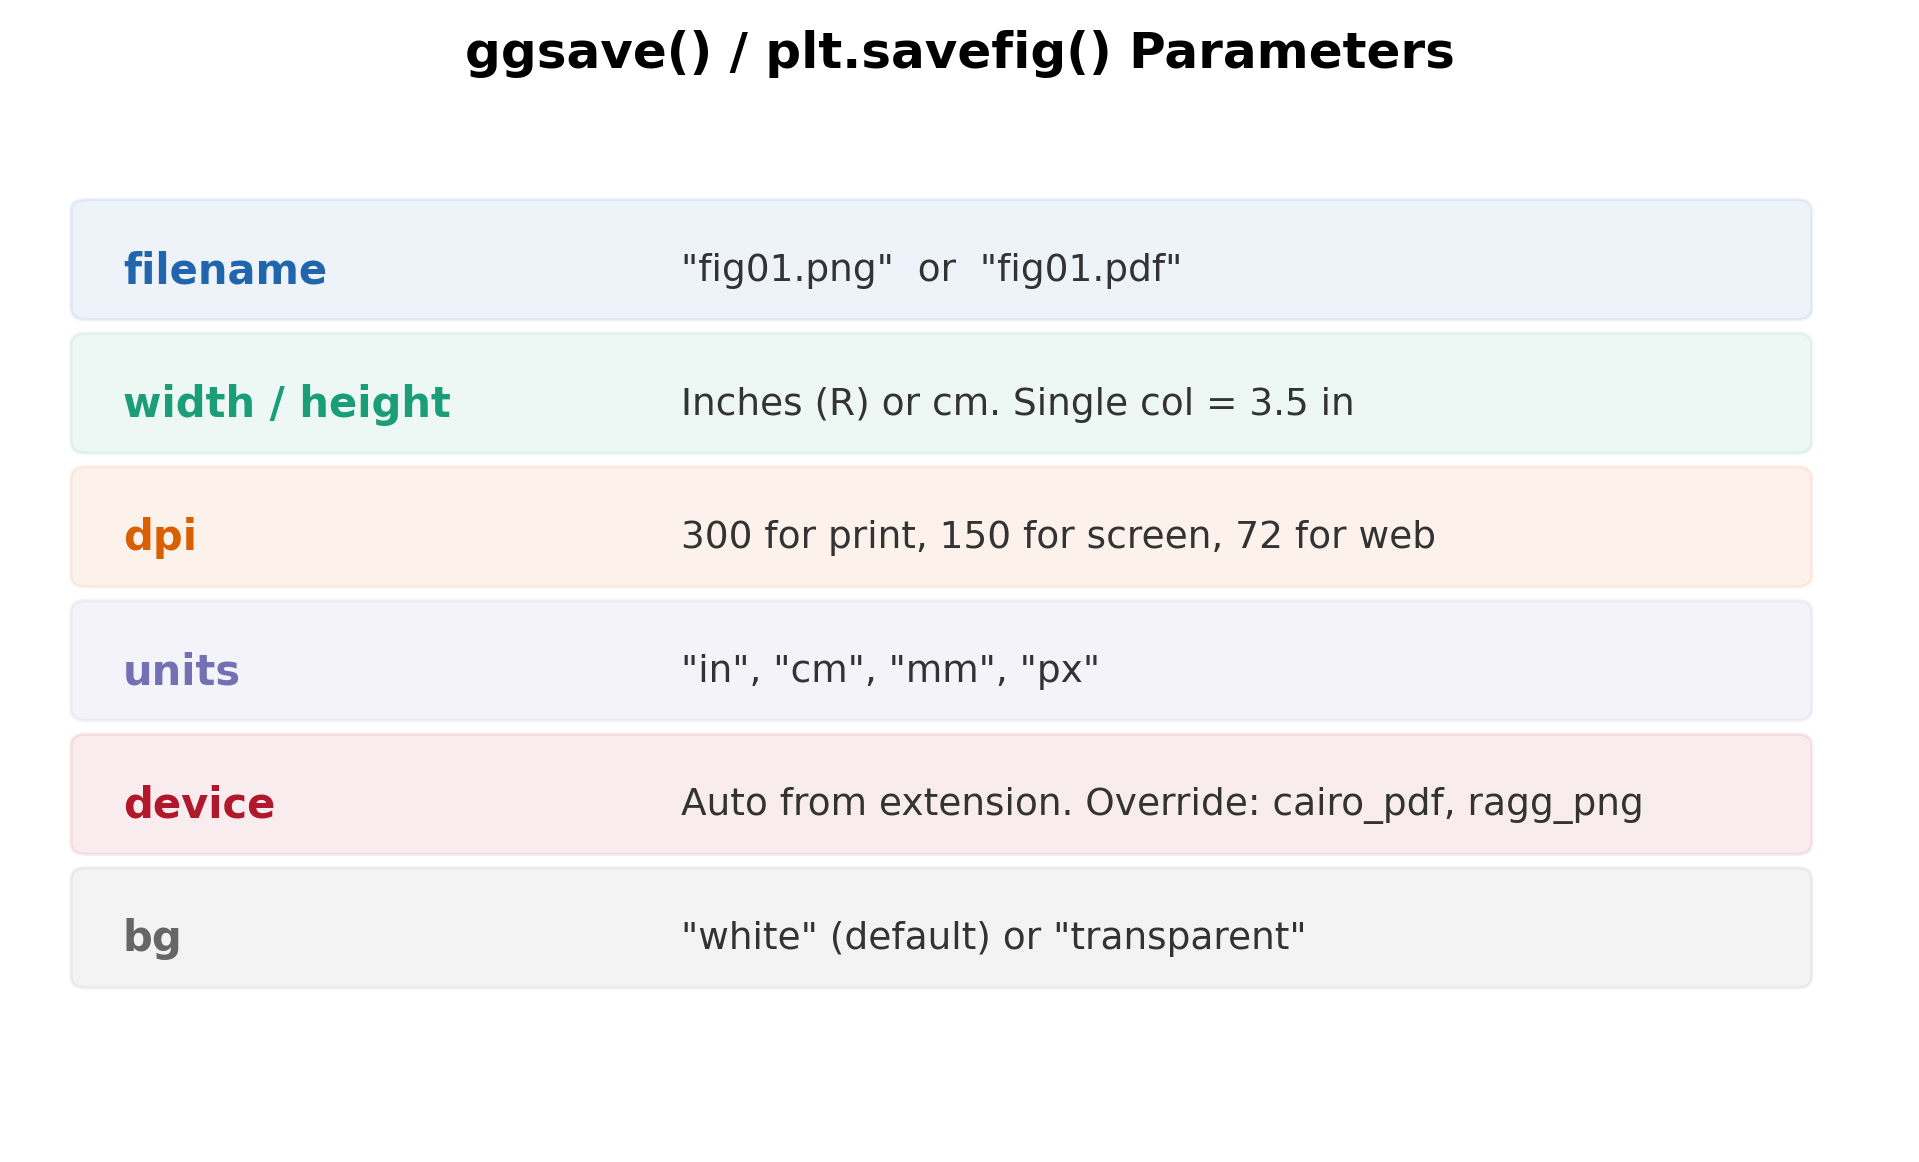
\includegraphics[width=0.78\textwidth]{m1_10_save_params.png}

\vspace{0.2cm}
\begin{exampleblock}{Data Insight}
    \scriptsize Always specify \texttt{width}, \texttt{height}, and \texttt{dpi} explicitly. The defaults use the current device/window dimensions, which are not reproducible across machines.
\end{exampleblock}
\end{frame}

% ── 276 ──
\begin{frame}[fragile]{\texttt{ggsave()} --- \Rlang}\smark{276/300}
\begin{columns}[T]
\begin{column}{0.55\textwidth}
\begin{lstlisting}[style=Rstyle]
p <- ggplot(penguins, aes(
    bill_length_mm, body_mass_g,
    color=species)) +
  geom_point() + theme_minimal()

# PNG for slides
ggsave("fig01.png", p,
  width=7, height=4.5,
  dpi=300, bg="white")

# PDF for journal
ggsave("fig01.pdf", p,
  width=3.5, height=2.5,
  device=cairo_pdf)

# SVG for web
ggsave("fig01.svg", p,
  width=7, height=4.5)
\end{lstlisting}
\end{column}
\begin{column}{0.42\textwidth}
\begin{alertblock}{Pro-Tip}
    \scriptsize \texttt{cairo\_pdf} embeds fonts properly (no missing glyphs). \texttt{ragg::agg\_png()} produces higher-quality raster than the default PNG device.
\end{alertblock}
\vspace{0.2cm}
\begin{exampleblock}{Data Insight}
    \scriptsize \texttt{bg="white"} ensures the background is opaque. Default is transparent in some devices, which looks broken when pasted into Word/PowerPoint.
\end{exampleblock}
\end{column}
\end{columns}
\end{frame}

% ── 277 ──
\begin{frame}[fragile]{\texttt{savefig()} --- \Python}\smark{277/300}
\begin{columns}[T]
\begin{column}{0.55\textwidth}
\begin{lstlisting}[style=Pystyle]
fig, ax = plt.subplots(
    figsize=(7, 4.5))  # inches
# ... plot code ...

# PNG for slides
fig.savefig("fig01.png",
    dpi=300, bbox_inches="tight",
    facecolor="white")

# PDF for journal
fig.savefig("fig01.pdf",
    bbox_inches="tight")

# SVG for web
fig.savefig("fig01.svg",
    bbox_inches="tight")

# plotnine
p.save("fig01.png",
    dpi=300, width=7, height=4.5)
\end{lstlisting}
\end{column}
\begin{column}{0.42\textwidth}
\begin{alertblock}{Pro-Tip}
    \scriptsize \texttt{bbox\_inches="tight"} crops whitespace. Without it, saved figures often have enormous margins. Always include this parameter.
\end{alertblock}
\vspace{0.2cm}
\begin{exampleblock}{Data Insight}
    \scriptsize \texttt{figsize=(w, h)} in \texttt{plt.subplots()} sets the size in inches at creation time. \texttt{dpi} in \texttt{savefig()} only affects raster output.
\end{exampleblock}
\end{column}
\end{columns}
\end{frame}

% ── 278 ──
\begin{frame}{Figure Sizing for Publication}
\smark{278/300}
\centering
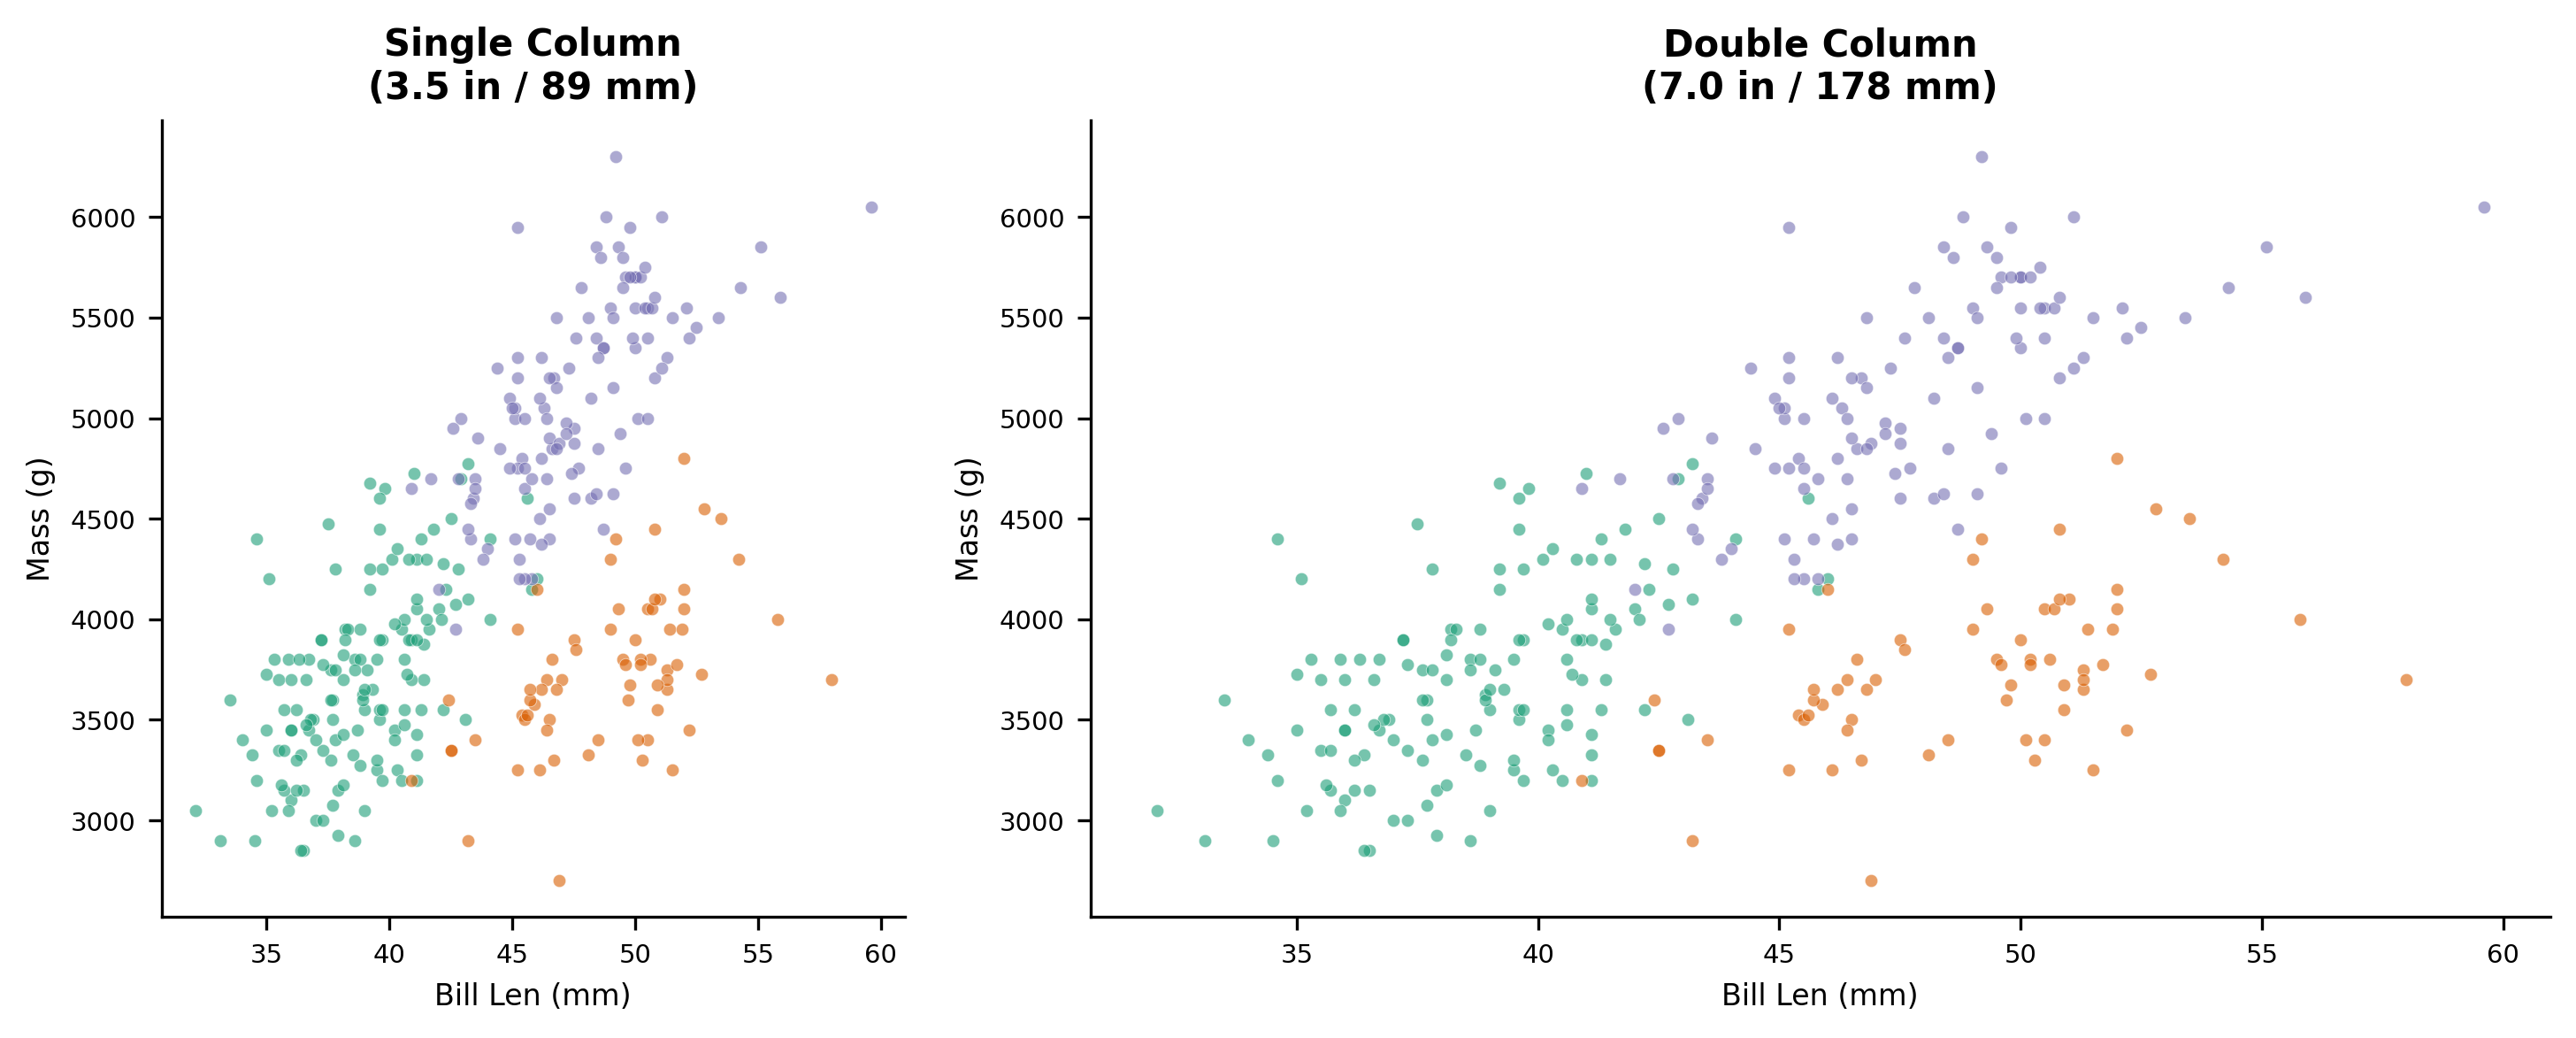
\includegraphics[width=0.85\textwidth]{m1_10_figure_sizing.png}

\vspace{0.2cm}
\centering\small
\begin{tabular}{@{}lrrl@{}}
    \toprule
    \textbf{Context} & \textbf{Width} & \textbf{Height} & \textbf{Notes} \\
    \midrule
    Journal single-col   & 3.5 in   & 2.5--3.0 in & Most common \\
    Journal double-col   & 7.0 in   & 3.5--5.0 in & Multi-panel \\
    Beamer slide         & 10.0 in  & 5.5 in      & \texttt{base\_size=16} \\
    PowerPoint           & 10.0 in  & 5.6 in      & 16:9 aspect \\
    Poster (A0)          & 12--18 in & variable    & \texttt{base\_size=20+} \\
    \bottomrule
\end{tabular}
\end{frame}

% ── 279 ──
\begin{frame}{Font Embedding in PDFs}
\smark{279/300}
\begin{columns}[T]
\begin{column}{0.50\textwidth}
\begin{itemize}
    \item Journals require \textbf{all fonts embedded}
    \item Missing fonts $\to$ substitution $\to$ broken labels
    \item R: \texttt{cairo\_pdf()} auto-embeds; base \texttt{pdf()} does not
    \item Python: matplotlib's PDF backend embeds by default
    \item Check: \texttt{pdffonts fig01.pdf} (Linux command)
\end{itemize}
\end{column}
\begin{column}{0.47\textwidth}
\begin{alertblock}{Pro-Tip}
    \scriptsize If a journal rejects your PDF for missing fonts, re-export with \texttt{device=cairo\_pdf} in R or set \texttt{plt.rcParams["pdf.fonttype"] = 42} in matplotlib (TrueType instead of Type 3).
\end{alertblock}
\end{column}
\end{columns}
\end{frame}

% ── 280 ──
\begin{frame}{Reproducible Project Structure}
\smark{280/300}
\centering
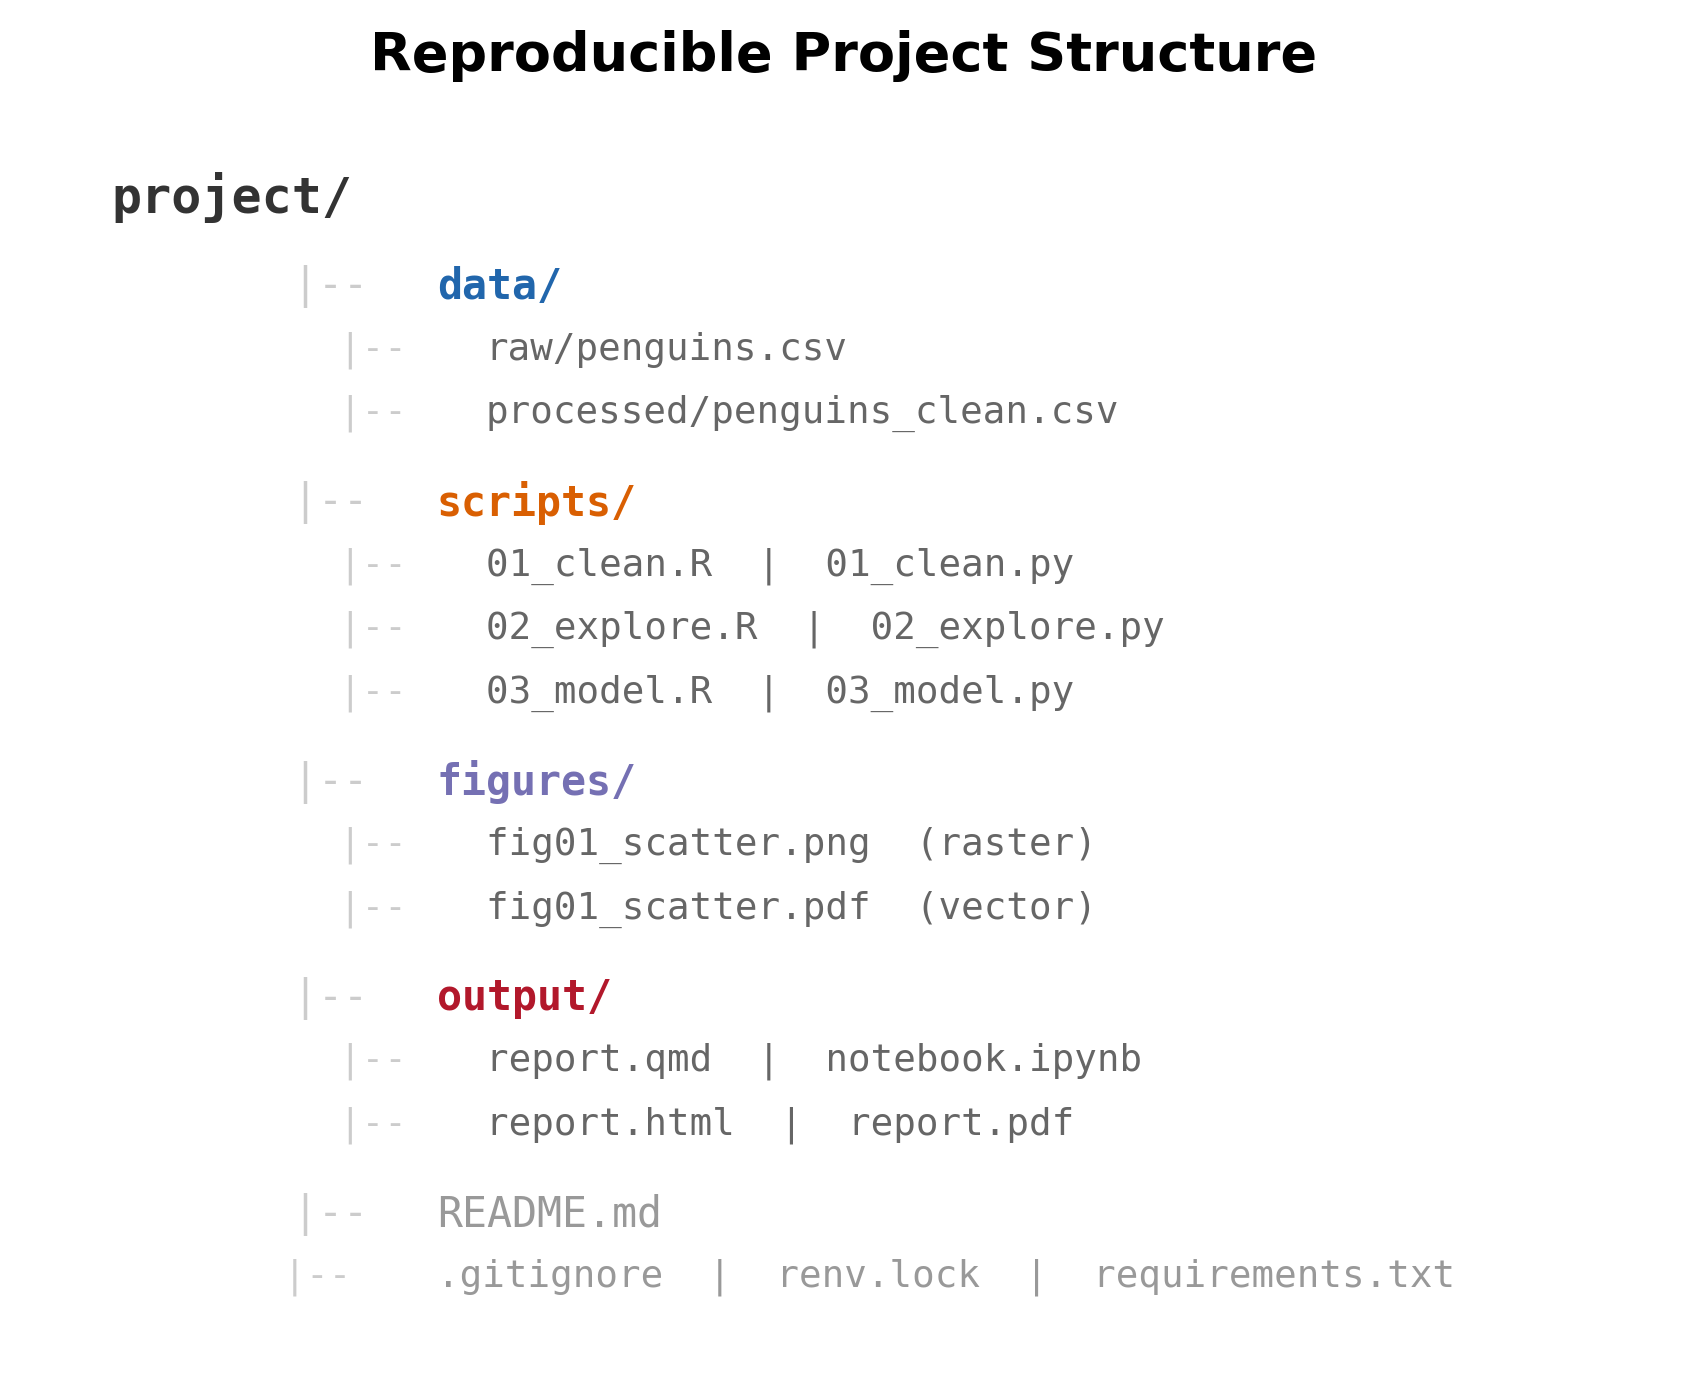
\includegraphics[width=0.62\textwidth]{m1_10_folder_structure.png}

\vspace{0.2cm}
\begin{exampleblock}{Data Insight}
    \scriptsize Numbered scripts (\texttt{01\_clean}, \texttt{02\_explore}) enforce execution order. Separate \texttt{data/raw} (immutable) from \texttt{data/processed} (derived). Figures get both raster and vector versions.
\end{exampleblock}
\end{frame}

% ── 281 ──
\begin{frame}{Reproducibility Principles for Figures}
\smark{281/300}
\begin{columns}[T]
\begin{column}{0.50\textwidth}
\begin{itemize}
    \item Every figure is generated by a \textbf{script}, never by clicking in a GUI
    \item Scripts run \textbf{top-to-bottom} without manual intervention
    \item Data paths are \textbf{relative}, not absolute
    \item Random seeds are set (\texttt{set.seed()} / \texttt{np.random.seed()})
\end{itemize}
\end{column}
\begin{column}{0.47\textwidth}
\begin{alertblock}{Pro-Tip}
    \scriptsize The test: can a colleague clone your repo, run one command, and regenerate all figures identically? If not, it is not reproducible.
\end{alertblock}
\vspace{0.2cm}
\begin{exampleblock}{Data Insight}
    \scriptsize Package versions matter. Lock them with \texttt{renv::snapshot()} (R) or \texttt{pip freeze > requirements.txt} (Python).
\end{exampleblock}
\end{column}
\end{columns}
\end{frame}

% ── 282 ──
\begin{frame}[fragile]{R Markdown / Quarto Figure Chunks}\smark{282/300}
\begin{columns}[T]
\begin{column}{0.55\textwidth}
\begin{lstlisting}[style=Rstyle,language={}]
```{r fig-scatter,
    fig.width=7,
    fig.height=4.5,
    fig.cap="Penguins scatter",
    dpi=300,
    dev="cairo_pdf"}

ggplot(penguins, aes(
    bill_length_mm,
    body_mass_g,
    color = species)) +
  geom_point() +
  theme_minimal()
```
\end{lstlisting}
\end{column}
\begin{column}{0.42\textwidth}
\begin{alertblock}{Pro-Tip}
    \scriptsize Chunk options control export: \texttt{fig.width}, \texttt{fig.height} (inches), \texttt{dpi}, \texttt{dev} (device). The figure is auto-saved and embedded in the output document.
\end{alertblock}
\vspace{0.2cm}
\begin{exampleblock}{Data Insight}
    \scriptsize Quarto uses YAML-style chunk options: \texttt{\#| fig-width: 7}. Same parameters, different syntax.
\end{exampleblock}
\end{column}
\end{columns}
\end{frame}

% ── 283 ──
\begin{frame}[fragile]{Jupyter Notebook Figures}\smark{283/300}
\begin{columns}[T]
\begin{column}{0.55\textwidth}
\begin{lstlisting}[style=Pystyle]
# Cell 1: Config (run once)
%matplotlib inline
%config InlineBackend \
  .figure_format = "retina"
# retina = 2x DPI for notebooks

# Cell 2: Plot
fig, ax = plt.subplots(
    figsize=(7, 4.5))
# ... plot code ...

# Cell 3: Export
fig.savefig("figures/fig01.png",
    dpi=300, bbox_inches="tight")
fig.savefig("figures/fig01.pdf",
    bbox_inches="tight")
\end{lstlisting}
\end{column}
\begin{column}{0.42\textwidth}
\begin{alertblock}{Pro-Tip}
    \scriptsize \texttt{\%config InlineBackend.figure\_format="retina"} doubles the inline resolution. Without it, notebook figures look blurry on HiDPI screens.
\end{alertblock}
\vspace{0.2cm}
\begin{exampleblock}{Data Insight}
    \scriptsize \texttt{plt.show()} renders inline. \texttt{fig.savefig()} writes to disk. Do both: show for review, save for reproducibility.
\end{exampleblock}
\end{column}
\end{columns}
\end{frame}

% ── 284 ──
\begin{frame}{Version Control for Figures}
\smark{284/300}
\begin{columns}[T]
\begin{column}{0.50\textwidth}
\begin{itemize}
    \item Track \textbf{scripts}, not \textbf{output PNGs} (binary files bloat Git)
    \item Add \texttt{figures/*.png} to \texttt{.gitignore}
    \item The script \emph{is} the figure's source of truth
    \item If you must track outputs: use Git LFS or DVC
    \item Naming convention: \texttt{fig01\_scatter\_species.png} (numbered + descriptive)
\end{itemize}
\end{column}
\begin{column}{0.47\textwidth}
\begin{alertblock}{Pro-Tip}
    \scriptsize Every figure script should be \textbf{self-contained}: load data, make plot, save to disk. No dependency on interactive session state.
\end{alertblock}
\vspace{0.2cm}
\begin{exampleblock}{Data Insight}
    \scriptsize Numbering figures (\texttt{fig01}, \texttt{fig02}) matches manuscript figure references and ensures they sort correctly in file browsers.
\end{exampleblock}
\end{column}
\end{columns}
\end{frame}

% ── 285 ──
\begin{frame}[fragile]{Batch Export: All Figures in One Script}\smark{285/300}
\begin{columns}[T]
\begin{column}{0.48\textwidth}
\begin{lstlisting}[style=Rstyle]
# make_figures.R
library(ggplot2)
source("theme_brand.R")
theme_set(theme_brand())

# Load data once
pen <- palmerpenguins::penguins

# Fig 1
p1 <- ggplot(pen, aes(...)) +
  geom_point()
ggsave("figures/fig01.pdf", p1,
  width=3.5, height=2.5)

# Fig 2
p2 <- ggplot(pen, aes(...)) +
  geom_histogram()
ggsave("figures/fig02.pdf", p2,
  width=3.5, height=2.5)

# Run: Rscript make_figures.R
\end{lstlisting}
\end{column}
\begin{column}{0.48\textwidth}
\begin{lstlisting}[style=Pystyle]
# make_figures.py
import matplotlib.pyplot as plt
from theme_brand import apply_brand

# Fig 1
fig, ax = plt.subplots(...)
apply_brand(fig, ax)
# ... plot ...
fig.savefig("figures/fig01.pdf")
plt.close()

# Fig 2
fig, ax = plt.subplots(...)
apply_brand(fig, ax)
# ... plot ...
fig.savefig("figures/fig02.pdf")
plt.close()

# Run: python make_figures.py
\end{lstlisting}
\end{column}
\end{columns}
\end{frame}

% ── 286 ──
\begin{frame}{Environment Locking}
\smark{286/300}
\centering\small
\begin{tabular}{@{}lll@{}}
    \toprule
    \textbf{Tool} & \textbf{Language} & \textbf{What It Locks} \\
    \midrule
    \texttt{renv}           & R      & Package versions, CRAN snapshot \\
    \texttt{groundhog}      & R      & Date-based package loading \\
    \texttt{pip freeze}     & Python & \texttt{requirements.txt} \\
    \texttt{conda env export}& Python & Full environment YAML \\
    \texttt{poetry.lock}    & Python & Exact dependency tree \\
    Docker                  & Both   & Entire OS + packages \\
    \bottomrule
\end{tabular}

\vspace{0.3cm}
\begin{exampleblock}{Data Insight}
    \scriptsize A figure rendered with \texttt{ggplot2 3.4.0} may look subtly different under \texttt{3.5.0} (default aesthetics change between versions). Locking prevents surprise diffs.
\end{exampleblock}
\end{frame}

% ── 287 ──
\begin{frame}{Parameterized Reports}
\smark{287/300}
\begin{columns}[T]
\begin{column}{0.50\textwidth}
\begin{itemize}
    \item One report template, multiple data inputs
    \item Quarto / R Markdown: YAML \texttt{params:} field
    \item Jupyter: \texttt{papermill} for parameterized notebooks
    \item Use case: monthly reports, client-specific dashboards, A/B test summaries
\end{itemize}
\end{column}
\begin{column}{0.47\textwidth}
\begin{alertblock}{Pro-Tip}
    \scriptsize Quarto: \texttt{quarto render report.qmd -P species:Gentoo} generates the Gentoo-specific version. One template $\to$ $n$ outputs. Workshop 9 covers this in depth.
\end{alertblock}
\vspace{0.2cm}
\begin{exampleblock}{Data Insight}
    \scriptsize Parameterized reports are the ``last mile'' of reproducibility: same code + different parameters = different figures, all auditable.
\end{exampleblock}
\end{column}
\end{columns}
\end{frame}

% ── 288 ──
\begin{frame}{Export Checklist}
\smark{288/300}
\centering\small
\begin{tabular}{@{}ll@{}}
    \toprule
    \textbf{Check} & \textbf{Action} \\
    \midrule
    Width \& height set explicitly?       & \texttt{width=3.5, height=2.5} \\
    DPI $\geq$300 for raster?             & \texttt{dpi=300} \\
    Background opaque?                    & \texttt{bg="white"} / \texttt{facecolor="white"} \\
    Fonts embedded in PDF?                & Use \texttt{cairo\_pdf} / \texttt{pdf.fonttype=42} \\
    Labels readable at final size?        & Print at target column width \\
    Colorblind-safe palette?              & Test with \texttt{colorblindr} / simulator \\
    Script reproduces figure from scratch?& \texttt{Rscript make\_figures.R} \\
    Raster \& vector both saved?          & \texttt{.png} + \texttt{.pdf} \\
    \bottomrule
\end{tabular}
\end{frame}

% ── 289 ──
\begin{frame}{Module 1.10 --- Key Takeaways}\smark{289/300}
\begin{enumerate}
    \item \textbf{Vector for print, raster for screen.} Save both.
    \item \textbf{300 DPI minimum} for journal raster figures.
    \item \textbf{Always specify width, height, dpi.} Never rely on defaults.
    \item \textbf{Every figure has a script.} The script is the source of truth.
    \item \textbf{Lock your environment.} \texttt{renv} / \texttt{requirements.txt} / Docker.
    \item \textbf{Numbered filenames} match manuscript references.
\end{enumerate}
\end{frame}

% ── 290 ──
\begin{frame}{}\smark{290/300}
\centering\vspace{1.5cm}
{\Large\textbf{Module 1.10 Complete}}\\[0.5cm]
You can now export publication-quality figures in any format, at any resolution, from reproducible scripts with locked environments.\\[0.5cm]
All 10 modules of Workshop 1 are done.
\end{frame}


% ═══════════════════════════════════════════════════════
%  WORKSHOP 1 — Summary and References (slides 291-300)
% ═══════════════════════════════════════════════════════
\section{Workshop 1 --- Summary and References}

% ── 291 ──
\begin{frame}{Workshop 1 --- The Complete Toolkit}
\smark{291/300}
\centering\small
\begin{tabular}{@{}cll@{}}
    \toprule
    \textbf{Module} & \textbf{Topic} & \textbf{Core Skill} \\
    \midrule
    1.1  & Perception \& Cognition     & Why we visualize; encoding hierarchy \\
    1.2  & Grammar of Graphics         & 7-component framework \\
    1.3  & Scatter, Bar, Line          & The 3 workhorse geoms \\
    1.4  & Histograms \& Density       & Univariate distribution shape \\
    1.5  & Color, Shape, Size, Alpha   & Non-positional aesthetic mapping \\
    1.6  & Faceting \& Small Multiples & Panel decomposition \\
    1.7  & Coordinate Systems          & Log, polar, flip, zoom \\
    1.8  & Themes \& Typography        & Visual identity \\
    1.9  & Annotation \& Storytelling  & Explanatory figures \\
    1.10 & Export \& Reproducibility   & Publication workflow \\
    \bottomrule
\end{tabular}
\end{frame}

% ── 292 ──
\begin{frame}{Workshop 1 --- The 10 Commandments}
\smark{292/300}
\begin{enumerate}
    \item \textbf{Always plot your data.} Statistics hide structure.
    \item \textbf{Design for preattentive pop-out.} Color the message; grey the context.
    \item \textbf{Respect the encoding hierarchy.} Position $>$ Length $>$ Angle $>$ Area.
    \item \textbf{Tidy data first.} One variable per column, one observation per row.
    \item \textbf{Mapping $\neq$ setting.} Inside \texttt{aes()} is data-driven.
    \item \textbf{Diagnose overplotting early.} Alpha, jitter, density.
    \item \textbf{Facet instead of overloading color.} Small multiples scale better.
    \item \textbf{Title = insight, not description.} State the conclusion.
    \item \textbf{Test for colorblindness.} Viridis, Okabe--Ito, redundant encoding.
    \item \textbf{Script every figure.} Reproducibility is non-negotiable.
\end{enumerate}
\end{frame}

% ── 293 ──
\begin{frame}{R Ecosystem Summary}
\smark{293/300}
\centering\small
\begin{tabular}{@{}ll@{}}
    \toprule
    \textbf{Package} & \textbf{Role} \\
    \midrule
    \texttt{ggplot2}          & Grammar of graphics engine \\
    \texttt{scales}           & Axis formatting, palettes \\
    \texttt{forcats}          & Factor reordering \\
    \texttt{ggrepel}          & Non-overlapping text labels \\
    \texttt{patchwork}        & Multi-panel composition \\
    \texttt{ggthemes}         & Extension themes \\
    \texttt{palmerpenguins}   & Teaching dataset \\
    \texttt{ragg}             & High-quality PNG device \\
    \texttt{showtext}         & Custom fonts \\
    \texttt{renv}             & Environment locking \\
    \bottomrule
\end{tabular}
\end{frame}

% ── 294 ──
\begin{frame}{Python Ecosystem Summary}
\smark{294/300}
\centering\small
\begin{tabular}{@{}ll@{}}
    \toprule
    \textbf{Package} & \textbf{Role} \\
    \midrule
    \texttt{plotnine}        & Grammar of graphics (ggplot2 port) \\
    \texttt{matplotlib}      & Low-level rendering engine \\
    \texttt{seaborn}         & Statistical visualization API \\
    \texttt{pandas}          & Data wrangling + basic plotting \\
    \texttt{numpy}           & Numerical computation \\
    \texttt{scipy.stats}     & KDE, QQ plots, distributions \\
    \texttt{adjustText}      & Non-overlapping labels \\
    \texttt{palmerpenguins}  & Teaching dataset \\
    \texttt{SciencePlots}    & Journal-style themes \\
    \bottomrule
\end{tabular}
\end{frame}

% ── 295 ──
\begin{frame}{What Comes Next: Workshops 2--9}
\smark{295/300}
\centering\small
\begin{tabular}{@{}cl@{}}
    \toprule
    \textbf{Workshop} & \textbf{Topic} \\
    \midrule
    2 & Statistical Visualization: inference, uncertainty, model diagnostics \\
    3 & Categorical \& Compositional Data: bars, treemaps, Sankey \\
    4 & Time Series \& Temporal Patterns: lines, decomposition, animation \\
    5 & Multivariate \& High-Dimensional: PCA, t-SNE, heatmaps \\
    6 & Geospatial Visualization: choropleths, Leaflet, cartograms \\
    7 & Network \& Hierarchical Data: graphs, dendrograms \\
    8 & Interactivity \& Dashboards: Plotly, Shiny, Streamlit \\
    9 & Publication Quality \& Advanced Topics: 3D, NLP, domain showcases \\
    \bottomrule
\end{tabular}
\end{frame}

% ── 296 ──
\begin{frame}{Recommended Reading}
\smark{296/300}
\small
\begin{itemize}
    \item Wilke, C.\ O.\ (2019). \textit{Fundamentals of Data Visualization}. O'Reilly. \textbf{Free online:} \texttt{clauswilke.com/dataviz}
    \item Healy, K.\ (2018). \textit{Data Visualization: A Practical Introduction}. Princeton UP. \textbf{Free online:} \texttt{socviz.co}
    \item Knaflic, C.\ N.\ (2015). \textit{Storytelling with Data}. Wiley.
    \item Wickham, H.\ (2016). \textit{ggplot2: Elegant Graphics for Data Analysis}. 2nd ed. Springer.
    \item Munzner, T.\ (2014). \textit{Visualization Analysis and Design}. A K Peters/CRC.
\end{itemize}
\end{frame}

% ── 297 ──
\begin{frame}{References (1/2)}
\smark{297/300}
\small
\begin{itemize}
    \item Anscombe, F.\ J.\ (1973). Graphs in statistical analysis. \textit{The American Statistician}, 27(1), 17--21.
    \item Borland, D., \& Taylor, R.\ M.\ (2007). Rainbow color map (still) considered harmful. \textit{IEEE CG\&A}, 27(2), 14--17.
    \item Cleveland, W.\ S., \& McGill, R.\ (1984). Graphical perception: Theory, experimentation, and application to the development of graphical methods. \textit{JASA}, 79(387), 531--554.
    \item Cleveland, W.\ S.\ (1993). \textit{Visualizing Data}. Hobart Press.
    \item Heer, J., \& Bostock, M.\ (2010). Crowdsourcing graphical perception. \textit{CHI~'10}, 203--212.
    \item Mackinlay, J.\ (1986). Automating the design of graphical presentations of relational information. \textit{ACM TOG}, 5(2), 110--141.
\end{itemize}
\end{frame}

% ── 298 ──
\begin{frame}{References (2/2)}
\smark{298/300}
\small
\begin{itemize}
    \item Matejka, J., \& Fitzmaurice, G.\ (2017). Same stats, different graphs: Generating datasets with varied appearance and identical statistics through simulated annealing. \textit{CHI~'17}.
    \item Simons, D.\ J., \& Chabris, C.\ F.\ (1999). Gorillas in our midst: Sustained inattentional blindness for dynamic events. \textit{Perception}, 28(9), 1059--1074.
    \item Tufte, E.\ R.\ (2001). \textit{The Visual Display of Quantitative Information}. 2nd ed. Graphics Press.
    \item Tukey, J.\ W.\ (1977). \textit{Exploratory Data Analysis}. Addison-Wesley.
    \item Wickham, H.\ (2010). A layered grammar of graphics. \textit{JCGS}, 19(1), 3--28.
    \item Wickham, H.\ (2014). Tidy data. \textit{Journal of Statistical Software}, 59(10).
    \item Wilkinson, L.\ (2005). \textit{The Grammar of Graphics}. 2nd ed. Springer.
\end{itemize}
\end{frame}

% ── 299 ──
\begin{frame}{Acknowledgments}
\smark{299/300}
\begin{columns}[T]
\begin{column}{0.50\textwidth}
    \textbf{Datasets used:}
    \begin{itemize}
        \item Palmer Penguins (Horst, Hill \& Gorman, 2020)
        \item Iris (Fisher, 1936 / Anderson, 1935)
        \item Diamonds, mpg, economics (ggplot2 built-ins)
        \item Anscombe's Quartet (Anscombe, 1973)
    \end{itemize}
\end{column}
\begin{column}{0.47\textwidth}
    \textbf{Tools:}
    \begin{itemize}
        \item R + ggplot2 ecosystem
        \item Python + plotnine + matplotlib + seaborn
        \item \LaTeX\ Beamer (metropolis theme)
        \item Fira Sans / Fira Mono typefaces
    \end{itemize}
\end{column}
\end{columns}
\end{frame}

% ── 300 ──
\begin{frame}{}
\smark{300/300}
\centering\vspace{1.5cm}
{\Huge\textbf{Workshop 1 Complete}}\\[0.8cm]
{\Large 300 slides $\cdot$ 10 modules $\cdot$ Comparative R \& Python}\\[0.8cm]
\textbf{Next workshop:} Statistical Visualization ---\\Inference, Uncertainty, and Model Diagnostics.
\end{frame}


\end{document}
